\documentclass[12pt,a4paper]{article}

% =============================
% Suppress warnings immediately
% =============================
\hfuzz=\maxdimen      % ignore small overfull boxes
\hbadness=10000       % no warnings for hboxes
\vbadness=10000       % no warnings for vboxes
\vfuzz=\maxdimen
\setlength{\overfullrule}{0pt} % no black bars
\sloppy                % allow flexible line breaking

% Suppress LaTeX warning commands
\makeatletter
\def\@warning#1{\relax}
\def\@latex@warning#1{\relax}
\def\@latex@warning@no@line#1{\relax}
\def\errmessage#1{}      % suppress TeX primitive errors
\def\wlog#1{}            % suppress log messages
\makeatother

% =============================
% Load preamble and macros
% =============================
% =============================
% Document class & basic setup
% =============================

% chktex-file 8

% Suppress underfull/overfull hbox warnings
\hbadness=10000
\hfuzz=\maxdimen
\vbadness=10000
\vfuzz=\maxdimen

% Encoding and fonts
\usepackage{everypage-1x}
\usepackage[T1]{fontenc}
\usepackage{lmodern}
\usepackage[protrusion=false]{microtype}       % Better typography
\renewcommand{\familydefault}{\sfdefault} % Sans serif default
% =============================
% Core packages
% =============================
\usepackage{graphicx}
\usepackage{subcaption}
\usepackage[table]{xcolor}
\usepackage{booktabs}
\usepackage{tabularx}
\usepackage{longtable}
\usepackage{wrapfig}
\usepackage[export]{adjustbox}
\usepackage[hidelinks]{hyperref}
\setlength{\headheight}{53.54352pt} % Fix fancyhdr warning
\usepackage{titlesec}
\usepackage{tocbibind}
\usepackage[most]{tcolorbox}
\usepackage{makeidx}
\usepackage{tikz}
\usetikzlibrary{calc}
\usepackage{geometry}
\usepackage{fancyhdr}
% =============================
% Geometry & margins
% =============================
\geometry{
  top=3.5cm,
  bottom=2.5cm,
  left=3cm,
  right=3cm,
  headsep=0.75cm
}
\newcommand{\sectionbreak}{\clearpage}
\newcommand{\subsectionbreak}{\clearpage}

\titlespacing*{\section}{0pt}{*2}{*1}
\titlespacing*{\subsection}{0pt}{*1.5}{*1}


% =============================
% Team branding colors
% =============================
\definecolor{teamprimary}{HTML}{862633}
\definecolor{teamsecondary}{HTML}{EAAA00}
\definecolor{textgray}{gray}{0.5}
% =============================
% Index setup
% =============================
\makeindex
\newcommand{\idx}[1]{#1\index{#1}}
% =============================
% Header & footer styles
% =============================
\newcommand{\teamname}{Claremont-Mudd-Scripps}
\newcommand{\sport}{Swim \& Dive}
\newcommand{\season}{2025--2026 Media Guide}
\newcommand{\teamlogo}{../assets/logo.png} % Path to logo
% Track current section/subsection
\newcommand{\currentsectiontitle}{}
\newcommand{\currentsubsectiontitle}{}
\renewcommand{\sectionmark}[1]{\gdef\currentsectiontitle{#1}}
\renewcommand{\subsectionmark}[1]{\gdef\currentsubsectiontitle{#1}}
\pagestyle{fancy}
\fancyhf{}
\fancyhead[L]{\fontsize{18pt}{30pt}\selectfont \teamname}
\fancyhead[R]{\fontsize{18pt}{30pt}\selectfont \season}
\fancyhead[C]{\raisebox{-0.2\height}{\includegraphics[height=1cm]{\teamlogo}}}
\fancyfoot[C]{\fontsize{12pt}{30pt}\selectfont \thepage}
\fancyfoot[L]{\textcolor{textgray}{\currentsectiontitle}}
\fancyfoot[R]{\textcolor{textgray}{\currentsubsectiontitle}}
\renewcommand{\headrule}{\vspace{5pt}\hrule height 0.4pt \vspace{5pt}}
% =============================
% Page border
% =============================
\newcommand\DrawPageBorder{%
\begin{tikzpicture}[overlay, remember picture]
\draw[teamprimary, line width=5pt] 
  ($(current page.north west) + (1cm,-1cm)$) rectangle 
  ($(current page.south east) + (-1cm,1cm)$);
\end{tikzpicture}%
}
\AddEverypageHook{\DrawPageBorder}
% =============================
% Custom commands
% =============================
\newcommand{\coachinfo}[4]{
    \begin{tcolorbox}[width=\textwidth, colback=teamsecondary!50!white, colframe=teamprimary, title=#1]
        \begin{tabularx}{\textwidth}[t]{@{}cX@{}}
            \raisebox{-\totalheight}{\includegraphics[height=2cm]{#2}} & 
            \begin{tabular}[t]{@{}lX@{}}
                \textbf{#3} \\
                #4
            \end{tabular}
        \end{tabularx}
    \end{tcolorbox}
    \vspace{10pt}
}
% =============================
% Hypersetup
% =============================
\hypersetup{
    colorlinks=true,
    linkcolor=black,
    urlcolor=black,
    unicode=true,
    breaklinks=true,
    pdfstartview=FitH
}
% chktex-file 44

% Required packages for table coloring
\usepackage{colortbl}

% Event Profile Table Macro
\newcommand{\eventprofiletable}[2]{
\begin{table}[H]
\centering
\caption*{\textbf{\textcolor{teamprimary}{#1}}}
\resizebox{\textwidth}{!}{%
\begin{tabular}{c | cccc | cccc}
\toprule
\rowcolor{teamprimary!25}
\textbf{Year} & \multicolumn{4}{c|}{\textbf{Prelims}} & \multicolumn{4}{c}{\textbf{Finals}} \\ 
\rowcolor{teamprimary!25}
 & \textbf{1st} & \textbf{8th} & \textbf{9th} & \textbf{16th} & \textbf{1st} & \textbf{8th} & \textbf{9th} & \textbf{16th} \\
\midrule
#2
\bottomrule
\end{tabular}%
}
\end{table}
}

% Awards Table Macro
\newcommand{\awardstable}[3]{
\begin{longtable}{#1}
\caption*{\textbf{\textcolor{teamprimary}{#2}}} \\
\toprule
\rowcolor{teamprimary!25}
#3 \\
\midrule
\endfirsthead

\toprule
\rowcolor{teamprimary!25}
#3 \\
\midrule
\endhead

\bottomrule
\endfoot
}

% Single Awards Table Macro
\newcommand{\awardstablesingle}[3]{
\begin{table}[htbp]
\centering
\caption*{\textbf{\textcolor{teamprimary}{#1}}}
\resizebox{\textwidth}{!}{%
\begin{tabular}{#2}
\toprule
\rowcolor{teamprimary!25}
#3 \\
\midrule
}

% Close single awards table
\newcommand{\awardstablesingleclose}{
\bottomrule
\end{tabular}%
}
\end{table}
}

% Team Record Table Macro (for minipages)
\newcommand{\teamrecordtable}[2]{
\centering
\caption*{\textbf{\textcolor{teamprimary}{#1}}}
\resizebox{\textwidth}{!}{%
\renewcommand{\arraystretch}{1.25}
\begin{tabular}{@{}p{1.8cm}p{2.8cm}p{1.2cm}@{}}
\toprule
\rowcolor{teamprimary!25}
    \textbf{Time} & \textbf{Name} & \textbf{Year} \\
\midrule
#2
\bottomrule
\end{tabular}%
}
}

% Team Record Table Macro (for minipages)
\newcommand{\teamdivetable}[2]{
\centering
\caption*{\textbf{\textcolor{teamprimary}{#1}}}
\resizebox{\textwidth}{!}{%
\renewcommand{\arraystretch}{1.25}
\begin{tabular}{@{}p{1.8cm}p{2.8cm}p{1.2cm}@{}}
\toprule
\rowcolor{teamprimary!25}
    \textbf{Score} & \textbf{Name} & \textbf{Year} \\
\midrule
#2
\bottomrule
\end{tabular}%
}
}

% Team Record Table with Team column (for minipages)
\newcommand{\teamrecordtablewithteam}[2]{
\centering
\caption*{\textbf{\textcolor{teamprimary}{#1}}}
\resizebox{\textwidth}{!}{%
\renewcommand{\arraystretch}{1.1}
\begin{tabular}{@{}p{1.8cm}p{2.8cm}p{1.2cm}p{1.4cm}@{}}
\toprule
\rowcolor{teamprimary!25}
    \textbf{Time} & \textbf{Name} & \textbf{Year} & \textbf{Team} \\
\midrule
#2
\bottomrule
\end{tabular}%
}
}

% Team Record Table with Site column (for minipages)
\newcommand{\teamrecordtablewithsite}[2]{
\centering
\caption*{\textbf{\textcolor{teamprimary}{#1}}}
\resizebox{\textwidth}{!}{%
\renewcommand{\arraystretch}{2}
\begin{tabular}{@{}p{1.8cm}p{5.5cm}p{1.2cm}p{1.4cm}@{}}
\toprule
\rowcolor{teamprimary!25}
    \textbf{Time} & \textbf{Name} & \textbf{Year} & \textbf{Site} \\
\midrule
#2
\bottomrule
\end{tabular}%
}
}

% Team Record Table with full context (for minipages)
\newcommand{\teamrecordtablefull}[2]{
\centering
\caption*{\textbf{\textcolor{teamprimary}{#1}}}
\resizebox{\textwidth}{!}{%
\renewcommand{\arraystretch}{1.1}
\begin{tabular}{@{}p{1.8cm}p{2.8cm}p{1.2cm}p{1.4cm}p{1.4cm}p{2.0cm}@{}}
\toprule
\rowcolor{teamprimary!25}
    \textbf{Time} & \textbf{Name} & \textbf{Year} & \textbf{Site} & \textbf{Meet} & \textbf{Context} \\
\midrule
#2
\bottomrule
\end{tabular}%
}
}

% Team Record Development Table (for detailed records with context)
\newcommand{\teamrecorddevtable}[2]{%
\begin{table}[H]
\centering
\caption*{\textbf{\textcolor{teamprimary}{#1}}}
\scriptsize
\resizebox{\textwidth}{!}{%
\renewcommand{\arraystretch}{1}%
\begin{tabular}{@{}p{1.2cm}p{2.2cm}p{1.0cm}p{1.2cm}p{1.2cm}p{2.5cm}@{}}
\toprule
\rowcolor{teamprimary!25}
\textbf{Time} & \textbf{Name} & \textbf{Date} & \textbf{Site} & \textbf{Meet} & \textbf{Context} \\
\midrule
#2
\bottomrule
\end{tabular}%
} % end resizebox
\end{table}%
} % end macro

% Professional full-page section start with team primary background
\newcommand{\fullpagesection}[2]{%
    \clearpage
    \thispagestyle{empty}
    
    % Increment section counter first
    \stepcounter{section}
    \sectionmark{#2}
    
    % Full page background in team primary
    \begin{tikzpicture}[overlay, remember picture]
        \fill[teamprimary] (current page.north west) rectangle (current page.south east);
    \end{tikzpicture}
    
    \vspace*{0.05\textheight}
    
    \begin{center}
        % Image with easy positioning
        \ifx\relax#1\relax
            % No image provided - skip this section
        \else
            \begin{tikzpicture}
                % Easy coordinates: (left-right, up-down)
                % (0,0) = bottom left, (16,10) = top right
                \node[anchor=center] at (10, 5) {#1};
            \end{tikzpicture}
            \vspace{2cm}
        \fi

        % Section title with custom styling and section number
        \begin{minipage}{0.9\textwidth}
            \centering
            {\fontsize{32pt}{40pt}\selectfont 
             \fontfamily{phv}\selectfont
             \textcolor{teamsecondary}{\bfseries \thesection\ #2}}
        \end{minipage}
        
    \end{center}
    
    \vspace*{\fill}
    \clearpage
    
    % Add to table of contents
    \addcontentsline{toc}{section}{\thesection\ #2}
}




% =============================
% Silence overfull boxes in tables
% =============================
\usepackage{etoolbox}
\newcommand{\SilenceAllTables}{%
  \hbadness=10000%
  \hfuzz=\maxdimen%
  \tolerance=10000%
  \emergencystretch=\maxdimen%
}
\AtBeginEnvironment{tabular}{\SilenceAllTables}
\AtBeginEnvironment{tabular*}{\SilenceAllTables}
\AtBeginEnvironment{array}{\SilenceAllTables}
\AtBeginEnvironment{longtable}{\SilenceAllTables}
\AtBeginEnvironment{tabularx}{\SilenceAllTables}

% =============================
% Document content
% =============================
\begin{document}

% Title page
\begin{titlepage}
    \thispagestyle{empty}
    
    % Full-page title image
    \begin{tikzpicture}[overlay, remember picture]
        \node[anchor=center] at (current page.center) {
            \includegraphics[width=\paperwidth, height=\paperheight, keepaspectratio=false]{../assets/TITLE.jpg}
        };
    \end{tikzpicture}
    
    % Add some content to ensure the page is created
    \mbox{}
    
\end{titlepage}

\clearpage

\begin{center}
    \vspace*{3cm}
    
    {\fontsize{48}{60}\selectfont \textbf{\textcolor{teamprimary}{OPPORTUNITY}}} \\[0.5cm]
    
    
    \vspace{2cm}
    
    \begin{minipage}{0.8\textwidth}
        \centering
        \fontsize{18}{26}\selectfont
        \textcolor{teamprimary!90}{
            \textit{``Great moments are born from great opportunity. And that's what you have here tonight... Now go out there and take it!''}
        }
        
        \vspace{0.8cm}
        
        {\large \textcolor{teamprimary!70}{— Kurt Russell as Herb Brooks, \textit{Miracle} (2004)}}
    \end{minipage}
\end{center}


% Table of contents
\clearpage
\tableofcontents

% Wrap all sections in a group so suppression is active
{%
% =============================================================================
% CHAMPIONSHIP & DUAL MEET INFORMATION
% =============================================================================

\section{Championship \& Dual Meet Information}

% =============================================================================
% SCORING SYSTEMS
% =============================================================================

\subsection{Scoring Systems}

\begin{table}[H]
\centering
\small
\begin{tabular}{|p{3.5cm}|p{4cm}|p{4cm}|}
\hline
\rowcolor{teamprimary!20}
\textbf{Meet Type} & \textbf{Individual Events} & \textbf{Relays} \\
\hline
\rowcolor{teamprimary!5}
Championship & 20-17-16-15-14-13-12-11, 9-7-6-5-4-3-2-1 & 40-34-32-30-28-26-24-22, 18-14-12-10-8-6-4-2 \\
\hline
\rowcolor{teamprimary!5}
Dual Meet & 9-4-3-2-1 (best 3 score) & 11-4-2 (best 2 score) \\
\hline
\end{tabular}
\end{table}

% =============================================================================
% CHAMPIONSHIP SCHEDULES
% =============================================================================

\subsection{Championship Schedules}

\begin{table}[H]
\centering
\caption*{SCIACs}
\small
\begin{tabular}{p{2.8cm} p{2.8cm} p{2.8cm} p{3.2cm}}
\toprule
\rowcolor{teamprimary!20}
\textbf{Wednesday} & \textbf{Thursday} & \textbf{Friday} & \textbf{Saturday} \\
\midrule
Diving & 500 Freestyle & 100 Butterfly & 1650 Freestyle \\
\rowcolor{teamprimary!5}
200 Medley Relay & 200 IM & 400 IM & 200 Backstroke \\
800 Free Relay & 50 Freestyle & 200 Freestyle & 100 Freestyle \\
\rowcolor{teamprimary!5}
 & 200 Free Relay & 100 Breaststroke & 200 Breaststroke \\
 &  & 100 Backstroke & 200 Butterfly \\
\rowcolor{teamprimary!5}
 &  & 400 Medley Relay & 400 Free Relay \\
\bottomrule
\end{tabular}
\end{table}

\begin{table}[H]
\centering
\caption*{NCAAs}
\small
\begin{tabular}{p{2.8cm} p{2.8cm} p{2.8cm} p{3.2cm}}
\toprule
\rowcolor{teamprimary!20}
\textbf{Wednesday} & \textbf{Thursday} & \textbf{Friday} & \textbf{Saturday} \\
\midrule
500 Freestyle & 400 IM & 200 Medley Relay & 1650 Freestyle \\
\rowcolor{teamprimary!5}
200 IM & 100 Butterfly & 200 Butterfly & 100 Freestyle \\
50 Freestyle & 200 Freestyle & 100 Backstroke & 200 Backstroke \\
\rowcolor{teamprimary!5}
Diving & Diving & 100 Breaststroke & 200 Breaststroke \\
400 Medley Relay & 200 Free Relay & Diving & Diving \\
\rowcolor{teamprimary!5}
 &  & 800 Free Relay & 400 Free Relay \\
\bottomrule
\end{tabular}
\end{table}

% =============================================================================
% DUAL MEET INFORMATION
% =============================================================================

\subsection{Dual Meet Event Order}

\begin{table}[H]
\centering
\small
\begin{tabular}{|p{5.5cm}|p{5.5cm}|}
\hline
\rowcolor{teamprimary!20}
\textbf{16-Event Format} & \textbf{13-Event Format} \\
\hline
\rowcolor{teamprimary!5}
\textit{W 1m / M 3m Diving} & \textit{W 1m / M 3m Diving} \\
200 Medley Relay & Medley Relay (200/400) \\
\rowcolor{teamprimary!5}
1000 Freestyle & 1000 or 1650 Freestyle \\
200 Freestyle & 200 Freestyle \\
\rowcolor{teamprimary!5}
100 Backstroke & 50 Freestyle \\
100 Breaststroke & 200 or 400 IM \\
\rowcolor{teamprimary!5}
200 Butterfly & 50 Freestyle \\
\textit{Break / W 3m / M 1m} & \textit{Break / W 3m / M 1m} \\
\rowcolor{teamprimary!5}
100 Freestyle & 100 or 200 Butterfly \\
200 Backstroke & 100 Freestyle \\
\rowcolor{teamprimary!5}
500 Freestyle & 100 or 200 Backstroke \\
\textit{Break} & 500 Freestyle \\
\rowcolor{teamprimary!5}
100 Butterfly & 100 or 200 Breaststroke \\
200 Breaststroke & \textit{Break} \\
\rowcolor{teamprimary!5}
200 IM & Freestyle Relay (200/400) \\
400 Freestyle Relay &  \\
\hline
\end{tabular}
\end{table}

% =============================================================================
% PARTICIPATION RULES
% =============================================================================

\subsection{Participation Rules}

\begin{table}[H]
\centering
\small
\begin{tabular}{|p{3cm}|p{4cm}|p{5cm}|}
\hline
\rowcolor{teamprimary!20}
\textbf{Format} & \textbf{Individual Events} & \textbf{Event Combinations} \\
\hline
\rowcolor{teamprimary!5}
16-event & Up to 4 total & 3 ind/1 relay or 2 ind/2 relay \\
\hline
\rowcolor{teamprimary!5}
13-event & Up to 3 total & 3 ind, 2 ind/1 relay, or 1 ind/2 relay \\
\hline
\end{tabular}
\end{table}
\clearpage
\section{NCAA D-III Qualifying Standards}

% --- MEN ---
\begin{table}[htbp]
\centering
\caption*{\textbf{\textcolor{teamprimary}{Men}}}
\renewcommand{\arraystretch}{1.2}
\scriptsize
\begin{tabularx}{\textwidth}{lccrrrrrr}
\toprule
\rowcolor{teamprimary!25}
\textbf{\textcolor{black}{Event}} & \textbf{\textcolor{black}{D-III ``A''}} & \textbf{\textcolor{black}{D-III ``B''}} & \textbf{\textcolor{black}{2025}} & \textbf{\textcolor{black}{2024}} & \textbf{\textcolor{black}{2023}} & \textbf{\textcolor{black}{2022}} & \textbf{\textcolor{black}{2020}} & \textbf{\textcolor{black}{2019}} \\
\midrule
\rowcolor{teamsecondary!12}
50 Freestyle & 19.46 & 20.37 & 20.14 & 20.16 & 20.23 & 20.27 & 20.35 & 20.37 \\
\rowcolor{teamprimary!8}
100 Freestyle & 43.33 & 45.02 & 44.39 & 44.51 & 44.63 & 44.66 & 44.83 & 44.86 \\
\rowcolor{teamsecondary!12}
200 Freestyle & 1:36.16 & 1:39.40 & 1:38.05 & 1:38.62 & 1:38.88 & 1:38.90 & 1:38.62 & 1:39.28 \\
\rowcolor{teamprimary!8}
500 Freestyle & 4:20.26 & 4:31.24 & 4:27.21 & 4:29.54 & 4:28.69 & 4:28.98 & 4:30.11 & 4:29.81 \\
\rowcolor{teamsecondary!12}
1650 Freestyle & 15:02.59 & 15:50.88 & 15:36.67 & 15:43.03 & 15:46.24 & 15:38.05 & 15:45.81 & 15:44.28 \\
\rowcolor{teamprimary!8}
100 Backstroke & 46.29 & 49.28 & 48.67 & 48.62 & 48.63 & 48.54 & 49.08 & 49.10 \\
\rowcolor{teamsecondary!12}
200 Backstroke & 1:42.02 & 1:49.01 & 1:47.09 & 1:47.52 & 1:47.45 & 1:47.80 & 1:47.81 & 1:48.17 \\
\rowcolor{teamprimary!8}
100 Breaststroke & 52.11 & 55.29 & 54.49 & 54.62 & 54.89 & 54.85 & 55.03 & 55.41 \\
\rowcolor{teamsecondary!12}
200 Breaststroke & 1:53.85 & 2:02.06 & 1:59.71 & 1:59.78 & 2:00.14 & 2:00.10 & 2:00.87 & 2:00.93 \\
\rowcolor{teamprimary!8}
100 Butterfly & 46.52 & 48.63 & 48.15 & 48.12 & 48.18 & 48.35 & 48.44 & 48.75 \\
\rowcolor{teamsecondary!12}
200 Butterfly & 1:43.96 & 1:49.88 & 1:48.12 & 1:48.62 & 1:48.71 & 1:48.82 & 1:48.89 & 1:49.34 \\
\rowcolor{teamprimary!8}
200 IM & 1:44.94 & 1:50.25 & 1:48.95 & 1:49.24 & 1:49.42 & 1:49.64 & 1:50.17 & 1:50.70 \\
\rowcolor{teamsecondary!12}
400 IM & 3:47.19 & 3:58.93 & 3:54.62 & 3:56.33 & 3:57.03 & 3:57.21 & 3:56.71 & 3:56.64 \\
\rowcolor{teamprimary!8}
200 Medley Relay & --- & 1:29.60 & 1:28.38 & 1:28.93 & 1:29.38 & 1:29.35 & 1:30.00 & 1:29.94 \\
\rowcolor{teamsecondary!12}
400 Medley Relay & --- & 3:18.26 & 3:15.93 & 3:16.85 & 3:17.72 & 3:18.14 & 3:18.16 & 3:19.23 \\
\rowcolor{teamprimary!8}
200 Free Relay & --- & 1:21.55 & 1:20.86 & 1:21.10 & 1:21.30 & 1:21.32 & 1:21.76 & 1:22.02 \\
\rowcolor{teamsecondary!12}
400 Free Relay & --- & 3:01.31 & 2:59.71 & 3:00.30 & 3:00.61 & 3:00.30 & 3:01.26 & 3:01.77 \\
\rowcolor{teamprimary!8}
800 Free Relay & --- & 6:40.49 & 6:36.90 & 6:37.94 & 6:40.55 & 6:39.35 & 6:42.91 & 6:43.52 \\
\bottomrule
\end{tabularx}

\vspace{0.5em}
\small{1-Meter Diving Points—Dual 275 / Championship 425 \\
3-Meter Diving Points—Dual 285 / Championship 440}
\end{table}

% --- WOMEN ---
\begin{table}[H]
\centering
\caption*{\textbf{\textcolor{teamprimary}{Women}}}
\renewcommand{\arraystretch}{1.2}
\scriptsize
\begin{tabularx}{\textwidth}{lccrrrrrr}
\toprule
\rowcolor{teamprimary!25}
\textbf{\textcolor{black}{Event}} & \textbf{\textcolor{black}{D-III ``A''}} & \textbf{\textcolor{black}{D-III ``B''}} & \textbf{\textcolor{black}{2025}} & \textbf{\textcolor{black}{2024}} & \textbf{\textcolor{black}{2023}} & \textbf{\textcolor{black}{2022}} & \textbf{\textcolor{black}{2020}} & \textbf{\textcolor{black}{2019}} \\
\midrule
\rowcolor{teamsecondary!12}
50 Freestyle & 22.65 & 23.57 & 23.40 & 23.53 & 23.48 & 23.55 & 23.58 & 23.49 \\
\rowcolor{teamprimary!8}
100 Freestyle & 49.31 & 51.42 & 51.04 & 51.28 & 51.31 & 51.27 & 51.34 & 51.37 \\
\rowcolor{teamsecondary!12}
200 Freestyle & 1:47.13 & 1:52.17 & 1:51.54 & 1:51.64 & 1:52.00 & 1:51.87 & 1:51.78 & 1:51.63 \\
\rowcolor{teamprimary!8}
500 Freestyle & 4:45.33 & 5:00.37 & 4:58.89 & 4:58.57 & 4:59.17 & 4:59.97 & 4:57.37 & 4:59.35 \\
\rowcolor{teamsecondary!12}
1650 Freestyle & 16:27.52 & 17:21.20 & 17:19.75 & 17:18.05 & 17:18.75 & 17:18.85 & 17:15.04 & 17:12.13 \\
\rowcolor{teamprimary!8}
100 Backstroke & 53.70 & 56.76 & 56.17 & 56.73 & 56.39 & 56.82 & 56.23 & 56.39 \\
\rowcolor{teamsecondary!12}
200 Backstroke & 1:55.94 & 2:03.17 & 2:02.09 & 2:03.08 & 2:02.67 & 2:02.84 & 2:02.15 & 2:02.99 \\
\rowcolor{teamprimary!8}
100 Breaststroke & 59.84 & 1:04.25 & 1:03.54 & 1:03.99 & 1:03.98 & 1:04.34 & 1:04.04 & 1:04.33 \\
\rowcolor{teamsecondary!12}
200 Breaststroke & 2:10.99 & 2:20.43 & 2:19.45 & 2:19.78 & 2:19.42 & 2:20.50 & 2:19.39 & 2:20.77 \\
\rowcolor{teamprimary!8}
100 Butterfly & 52.92 & 55.96 & 55.52 & 55.74 & 55.68 & 55.79 & 55.76 & 56.13 \\
\rowcolor{teamsecondary!12}
200 Butterfly & 1:56.90 & 2:05.01 & 2:03.93 & 2:04.49 & 2:04.94 & 2:04.51 & 2:03.95 & 2:04.46 \\
\rowcolor{teamprimary!8}
200 IM & 1:58.27 & 2:05.70 & 2:05.42 & 2:05.44 & 2:04.96 & 2:05.78 & 2:05.29 & 2:05.77 \\
\rowcolor{teamsecondary!12}
400 IM & 4:13.77 & 4:29.40 & 4:26.91 & 4:28.50 & 4:28.28 & 4:27.96 & 4:27.72 & 4:28.65 \\
\rowcolor{teamprimary!8}
200 Medley Relay & --- & 1:44.61 & 1:43.88 & 1:44.06 & 1:43.95 & 1:44.57 & 1:44.30 & 1:44.55 \\
\rowcolor{teamsecondary!12}
400 Medley Relay & --- & 3:50.46 & 3:48.38 & 3:49.31 & 3:48.82 & 3:50.23 & 3:50.33 & 3:49.90 \\
\rowcolor{teamprimary!8}
200 Free Relay & --- & 1:35.10 & 1:34.29 & 1:34.49 & 1:34.86 & 1:35.08 & 1:35.04 & 1:34.95 \\
\rowcolor{teamsecondary!12}
400 Free Relay & --- & 3:29.09 & 3:27.55 & 3:28.16 & 3:28.68 & 3:28.68 & 3:26.70 & 3:28.45 \\
\rowcolor{teamprimary!8}
800 Free Relay & --- & 7:38.31 & 7:34.48 & 7:33.95 & 7:35.07 & 7:38.17 & 7:33.91 & 7:35.32 \\
\bottomrule
\end{tabularx}

\vspace{0.5em}
\small{1-Meter Diving Points—Dual 255 / Championship 395 \\
3-Meter Diving Points—Dual 265 / Championship 410}
\end{table}

\section{Event Profiles}

\subsection{SCIACs}

\subsubsection{Men}

\textbf{100 Freestyle}

\begin{flushleft}
\begin{tabular}{|c|c|c|c|c|c|c|c|c|}
\hline
Year & \multicolumn{4}{c|}{Prelims} & \multicolumn{4}{c|}{Finals} \\
\cline{2-9}
& 1st & 8th & 9th & 16th & 1st & 8th & 9th & 16th \\
\hline
2025 & 44.54 & 46.08 & 46.09 & 46.88 & 44.54 & 46.34 & 45.78 & 47.06 \\
2024 & 45.29 & 46.11 & 46.17 & 46.66 & 44.76 & 48.27 & 45.68 & 47.04  \\
2023 & 45.47 & 46.40 & 46.44 & 46.94 & 45.10 & 46.49 & 46.38 & 47.50 \\
\hline
\end{tabular}
\end{flushleft}

\textbf{200 Freestyle}

\begin{flushleft}
\begin{tabular}{|c|c|c|c|c|c|c|c|c|}
\hline
Year & \multicolumn{4}{c|}{Prelims} & \multicolumn{4}{c|}{Finals} \\
\cline{2-9}
& 1st & 8th & 9th & 16th & 1st & 8th & 9th & 16th \\
\hline
2025 & 1:40.53 & 1:41.55 & 1:42.03 & 1:43.59 & 1:39.48 & 1:41.62 & 1:41.58 & 1:44.60 \\
2024 & 1:39.16 & 1:42.48 & 1:42.59 & 1:44.74 & 1:37.65 & 1:42.17 & 1:42.09 & 1:47.02 \\
2023 & 1:39.15 & 1:42.72 & 1:42.74 & 1:44.14 & 1:38.44 & 1:41.93 & 1:42.20 & 1:45.11 \\
\hline
\end{tabular}
\end{flushleft}

\textbf{500 Freestyle}

\begin{flushleft}
\begin{tabular}{|c|c|c|c|c|c|c|c|c|}
\hline
Year & \multicolumn{4}{c|}{Prelims} & \multicolumn{4}{c|}{Finals} \\
\cline{2-9}
& 1st & 8th & 9th & 16th & 1st & 8th & 9th & 16th \\
\hline
2025 & 4:30.49 & 4:38.93 & 4:40.91 & 4:45.17 & 4:25.13 & 4:42.02 & 4:38.27 & 4:47.86 \\
2024 & 4:30.61 & 4:37.28 & 4:37.67 & 4:44.81 & 4:24.75 & 4:35.74 & 4:34.49 & 4:42.06 \\
2023 & 4:29.98 & 4:35.51 & 4:36.12 & 4:41.02 & 4:26.87 & 4:34.94 & 4:35.98 & 4:41.76 \\
\hline
\end{tabular}
\end{flushleft}

\textbf{1650 Freestyle}

\begin{flushleft}
\begin{tabular}{|c|c|c|c|c|c|c|c|c|}
\hline
Year & \multicolumn{4}{c|}{Prelims} & \multicolumn{4}{c|}{Finals} \\
\cline{2-9}
& 1st & 8th & 9th & 16th & 1st & 8th & 9th & 16th \\
\hline
2025 &  &  &  &  & 15:22.23 & 16:23.46 & 16:25.89 & 17:47.59 \\
2024 &  &  &  &  & 15:26.81 & 16:21.36 & 16:45.61 & 18.04.71 \\
2023 &  &  &  &  & 15:30.01 & 16:34.96 & 16:49.35 & 17:54.34 \\
\hline
\end{tabular}
\end{flushleft}

\textbf{100 Back}

\begin{flushleft}
\begin{tabular}{|c|c|c|c|c|c|c|c|c|}
\hline
Year & \multicolumn{4}{c|}{Prelims} & \multicolumn{4}{c|}{Finals} \\
\cline{2-9}
& 1st & 8th & 9th & 16th & 1st & 8th & 9th & 16th \\
\hline
2025 & 49.55 & 51.95 & 52.00 & 53.12 & 48.90 & 52.74 & 51.35 & 54.78 \\
2024 & 49.59 & 51.39 & 51.79 & 53.36 & 49.08 & 51.08 & 50.80 & 53.23 \\
2023 & 50.35 & 51.78 & 52.05 & 54.37 & 48.74 & 52.08 & 51.27 & 54.88 \\
\hline
\end{tabular}
\end{flushleft}

\textbf{200 Back}

\begin{flushleft}
\begin{tabular}{|c|c|c|c|c|c|c|c|c|}
\hline
Year & \multicolumn{4}{c|}{Prelims} & \multicolumn{4}{c|}{Finals} \\
\cline{2-9}
& 1st & 8th & 9th & 16th & 1st & 8th & 9th & 16th \\
\hline
2025 & 1:49.85 & 1:53.75 & 1:54.07 & 2:00.86 & 1:47.65 & 1:55.11 & 1:53.43 & 2:00.28 \\
2024 & 1:50.34 & 1:53.17 & 1:54.07 & 1:57.39 & 1:47.54 & 1:53.92 & 1:52.82 & 1:58.64 \\
2023 & 1:50.43 & 1:54.92 & 1:55.94 & 1:59.16 & 1:48.46 & 1:53.91 & 1:55.10 & 1:58.64 \\
\hline
\end{tabular}
\end{flushleft}

\textbf{100 Breast}

\begin{flushleft}
\begin{tabular}{|c|c|c|c|c|c|c|c|c|}
\hline
Year & \multicolumn{4}{c|}{Prelims} & \multicolumn{4}{c|}{Finals} \\
\cline{2-9}
& 1st & 8th & 9th & 16th & 1st & 8th & 9th & 16th \\
\hline
2025 & 54.31 & 56.52 & 56.71 & 57.43 & 54.05 & 56.47 & 56.36 & 57.76 \\
2024 & 55.21 & 56.58 & 56.73 & 58.56 & 55.11 & 56.85 & 56.75 & 58.89 \\
2023 & 55.98 & 56.92 & 57.23 & 58.50 & 55.80 & 57.24 & 56.96 & 59.09 \\
\hline
\end{tabular}
\end{flushleft}

\textbf{200 Breast}

\begin{flushleft}
\begin{tabular}{|c|c|c|c|c|c|c|c|c|}
\hline
Year & \multicolumn{4}{c|}{Prelims} & \multicolumn{4}{c|}{Finals} \\
\cline{2-9}
& 1st & 8th & 9th & 16th & 1st & 8th & 9th & 16th \\
\hline
2025 & 2:00.15 & 2:05.13 & 2:05.19 & 2:08.34 & 1:59.43 & 2:13.00 & 2:02.04 & 2:06.92 \\
2024 & 2:01.55 & 2:06.32 & 2:06.81 & 2:13.45 & 1:59.90 & 2:05.74  & 2:05.39  & 2:13.49 \\
2023 & 2:00.29 & 2:04.89 & 2:05.44 & 2:10.38 & 1:59.13 & 2:06.26 & 2:01.18 & 2:15.97 \\
\hline
\end{tabular}
\end{flushleft}

\textbf{100 Fly}

\begin{flushleft}
\begin{tabular}{|c|c|c|c|c|c|c|c|c|}
\hline
Year & \multicolumn{4}{c|}{Prelims} & \multicolumn{4}{c|}{Finals} \\
\cline{2-9}
& 1st & 8th & 9th & 16th & 1st & 8th & 9th & 16th \\
\hline
2025 & 48.98 & 50.48 & 50.50 & 51.59 & 48.39 & 50.14 & 50.51 & 51.28 \\
2024 & 48.73 & 50.33 & 50.38 & 51.52 & 47.55 & 50.45 & 49.93 & 51.69 \\
2023 & 48.85 & 50.49 & 50.50 & 51.26 & 47.89 & 50.25 & 49.87 & 51.62 \\
\hline
\end{tabular}
\end{flushleft}

\textbf{200 Fly}

\begin{flushleft}
\begin{tabular}{|c|c|c|c|c|c|c|c|c|}
\hline
Year & \multicolumn{4}{c|}{Prelims} & \multicolumn{4}{c|}{Finals} \\
\cline{2-9}
& 1st & 8th & 9th & 16th & 1st & 8th & 9th & 16th \\
\hline
2025 & 1:49.14 & 1:54.01 & 1:54.12 & 1:56.88 & 1:48.57 & 1:55.78 & 1:54.45 & 1:58.71 \\
2024 & 1:48.90 & 1:53.14 & 1:53.16 & 1:56.43 & 1:45.75 & 2:00.42 & 1:52.88  & 1:57.79  \\
2023 & 1:48.87 & 1:52.94 & 1:53.87 & 1:57.04 & 1:47.26 & 1:54.12 & 1:51.81 & 1:57.36 \\
\hline
\end{tabular}
\end{flushleft}

\textbf{200 IM}

\begin{flushleft}
\begin{tabular}{|c|c|c|c|c|c|c|c|c|}
\hline
Year & \multicolumn{4}{c|}{Prelims} & \multicolumn{4}{c|}{Finals} \\
\cline{2-9}
& 1st & 8th & 9th & 16th & 1st & 8th & 9th & 16th \\
\hline
2025 & 1:50.34 & 1:53.15 & 1:53.65 & 1:54.94 & 1:49.14 & 1:53.73 & 1:52.11 & 1:54.73 \\
2024 & 1:49.70 & 1:52.04 & 1:52.23 & 1:54.12 & 1:46.56 & 1:52.88 & 1:51.28 & 1:55.20 \\
2023 & 1:50.34 & 1:53.19 & 1:53.28 & 1:55.64 & 1:48.74 & 1:54.48 & 1:53.18 & 1:56.71 \\
\hline
\end{tabular}
\end{flushleft}

\textbf{400 IM}

\begin{flushleft}
\begin{tabular}{|c|c|c|c|c|c|c|c|c|}
\hline
Year & \multicolumn{4}{c|}{Prelims} & \multicolumn{4}{c|}{Finals} \\
\cline{2-9}
& 1st & 8th & 9th & 16th & 1st & 8th & 9th & 16th \\
\hline
2025 & 4:00.65 & 4:07.25 & 4:07.35 & 4:20.78 & 3:58.62 & 4:15.36 & 4:03.43 & 4:27.11 \\
2024 & 3:58.36 & 4:06.72 & 4:08.30 & 4:22.75 & 3:55.53 & 4:09.61 & 4:03.46 & 4:29.72 \\
2023 & 4:02.04 & 4:11.25 & 4:13.61 & 4:22.67 & 3:53.15 & 4:10.36 & 4:10.09 & 4:25.91 \\
\hline
\end{tabular}
\end{flushleft}

\textbf{200 Medley Relay}

\begin{flushleft}
\begin{tabular}{|c|c|c|c|c|c|c|c|c|}
\hline
Year & \multicolumn{4}{c|}{Prelims} & \multicolumn{4}{c|}{Finals} \\
\cline{2-9}
& 1st & 8th & 9th & 16th & 1st & 8th & 9th & 16th \\
\hline
2025 &  &  &  &  & 1:28.38 & 1:42.65 & 1:32.42 & 1:39.34 \\
2024 &  &  &  &  & 1:28.94 & 1:41.32 & 1:30.47 & 1:44.55 \\
2023 &  &  &  &  & 1:29.82 & 1:40.62 & 1:31.14 & 1:51.70 \\
\hline
\end{tabular}
\end{flushleft}

\textbf{400 Medley Relay}

\begin{flushleft}
\begin{tabular}{|c|c|c|c|c|c|c|c|c|}
\hline
Year & \multicolumn{4}{c|}{Prelims} & \multicolumn{4}{c|}{Finals} \\
\cline{2-9}
& 1st & 8th & 9th & 16th & 1st & 8th & 9th & 16th \\
\hline
2025 &  &  &  &  & 3:17.51 & 3:46.18 & 3:22.84 & 3:31.24 \\
2024 &  &  &  &  & 3:16.28 & 3:48.62 & 3:18.96 & 4:00.66 \\
2023 &  &  &  &  & 3:17.81 & 3:32.56 & 3:22.63 & 3:55.80 \\
\hline
\end{tabular}
\end{flushleft}

\textbf{200 Free Relay}

\begin{flushleft}
\begin{tabular}{|c|c|c|c|c|c|c|c|c|}
\hline
Year & \multicolumn{4}{c|}{Prelims} & \multicolumn{4}{c|}{Finals} \\
\cline{2-9}
& 1st & 8th & 9th & 16th & 1st & 8th & 9th & 16th \\
\hline
2025 &  &  &  &  & 1:20.90 & 1:29.47 & 1:24.11 & 1:33.68 \\
2024 &  &  &  &  & 1:20.81 & 1:29.36 & 1:22.03 & 1:35.54 \\
2023 &  &  &  &  & 1:21.99 & 1:29.65 & 1:23.82 & 1:35.04 \\
\hline
\end{tabular}
\end{flushleft}

\textbf{400 Free Relay}

\begin{flushleft}
\begin{tabular}{|c|c|c|c|c|c|c|c|c|}
\hline
Year & \multicolumn{4}{c|}{Prelims} & \multicolumn{4}{c|}{Finals} \\
\cline{2-9}
& 1st & 8th & 9th & 16th & 1st & 8th & 9th & 16th \\
\hline
2025 &  &  &  &  & 2:59.73 & 3:20.40 & 3:03.81 & 3:23.24 \\
2024 &  &  &  &  & 2:57.52  & 3:16.36 & 3:02.76  & 3:32.55 \\
2023 &  &  &  &  & 3:00.58 & 3:14.97 & 3:04.69 & 3:26.50 \\
\hline
\end{tabular}
\end{flushleft}

\textbf{800 Free Relay}

\begin{flushleft}
\begin{tabular}{|c|c|c|c|c|c|c|c|c|}
\hline
Year & \multicolumn{4}{c|}{Prelims} & \multicolumn{4}{c|}{Finals} \\
\cline{2-9}
& 1st & 8th & 9th & 16th & 1st & 8th & 9th & 16th \\
\hline
2025 &  &  &  &  & 6:37.82 & 7:25.04 & 6:45.33 & 7:26.25 \\
2024 &  &  &  &  & 6:36.41 & 7:14.26 & 6:43.82 & 7:39.07 \\
2023 &  &  &  &  & 6:37.13 & 7:15.69 & 6:49.80 & 7:47.86 \\
\hline
\end{tabular}
\end{flushleft}

\subsubsection{Women}

\textbf{100 Freestyle}

\begin{flushleft}
\begin{tabular}{|c|c|c|c|c|c|c|c|c|}
\hline
Year & \multicolumn{4}{c|}{Prelims} & \multicolumn{4}{c|}{Finals} \\
\cline{2-9}
& 1st & 8th & 9th & 16th & 1st & 8th & 9th & 16th \\
\hline
2025 & 50.17 & 52.36 & 52.44 & 53.80 & 49.95 & 52.33 & 52.21 & 53.77 \\
2024 & 50.47 & 52.05 & 52.60 & 53.84 & 49.83  & 52.24 & 52.18  & 54.65  \\
2023 & 50.96 & 53.22 & 53.24 & 54.47 & 50.42 & 53.73 & 52.73 & 54.72 \\
\hline
\end{tabular}
\end{flushleft}

\textbf{200 Freestyle}

\begin{flushleft}
\begin{tabular}{|c|c|c|c|c|c|c|c|c|}
\hline
Year & \multicolumn{4}{c|}{Prelims} & \multicolumn{4}{c|}{Finals} \\
\cline{2-9}
& 1st & 8th & 9th & 16th & 1st & 8th & 9th & 16th \\
\hline
2025 & 1:51.28 & 1:55.84 & 1:56.23 & 1:59.10 & 1:49.78 & 1:55.53 & 1:56.32 & 1:59.42 \\
2024 & 1:51.64 & 1:55.85 & 1:56.33 & 1:59.61 & 1:51.92 & 1:55.66 & 1:56.39 & 2:00.83 \\
2023 & 1:53.08 & 1:55.89 & 1:56.35 & 1:58.94 & 1:52.15 & 1:54.92 & 1:55.35 & 1:58.86 \\
\hline
\end{tabular}
\end{flushleft}

\textbf{500 Freestyle}

\begin{flushleft}
\begin{tabular}{|c|c|c|c|c|c|c|c|c|}
\hline
Year & \multicolumn{4}{c|}{Prelims} & \multicolumn{4}{c|}{Finals} \\
\cline{2-9}
& 1st & 8th & 9th & 16th & 1st & 8th & 9th & 16th \\
\hline
2025 & 5:01.52 & 5:08.10 & 5:12.38 & 5:20.36 & 4:58.89 & 5:11.33 & 5:11.42 & 5:19.28 \\
2024 & 4:58.57 & 5:07.42 & 5:10.61 & 5:18.54 & 4:57.37 & 5:10.65 & 5:05.75 & 5:20.13 \\
2023 & 5:03.25 & 5:11.58 & 5:14.64 & 5:26.51 & 5:00.21 & 5:11.99 & 5:11.86 & 5:23.21 \\
\hline
\end{tabular}
\end{flushleft}

\textbf{1650 Freestyle}

\begin{flushleft}
\begin{tabular}{|c|c|c|c|c|c|c|c|c|}
\hline
Year & \multicolumn{4}{c|}{Prelims} & \multicolumn{4}{c|}{Finals} \\
\cline{2-9}
& 1st & 8th & 9th & 16th & 1st & 8th & 9th & 16th \\
\hline
2025 &  &  &  &  & 17:05.49 & 17:55.30 & 17:55.58 & 18:33.63 \\
2024 &  &  &  &  & 17:07.58 & 18:02.32 & 18:04.97 & 19:01.31 \\
2023 &  &  &  &  & 17:21.98 & 18:07.37 & 18:22.72 & 19:52.98 \\
\hline
\end{tabular}
\end{flushleft}

\textbf{100 Back}

\begin{flushleft}
\begin{tabular}{|c|c|c|c|c|c|c|c|c|}
\hline
Year & \multicolumn{4}{c|}{Prelims} & \multicolumn{4}{c|}{Finals} \\
\cline{2-9}
& 1st & 8th & 9th & 16th & 1st & 8th & 9th & 16th \\
\hline
2025 & 56.04 & 58.56 & 58.63 & 59.80 & 56.04 & 58.75 & 57.96 & 59.66 \\
2024 & 57.23 & 58.74 & 58.88 & 1:01.39 & 56.93 & 59.46 & 58.67 & 1:03.30 \\
2023 & 56.34 & 59.24 & 59.80 & 1:01.42 & 56.68 & 59.52 & 59.92 & 1:01.77 \\
\hline
\end{tabular}
\end{flushleft}

\textbf{200 Back}

\begin{flushleft}
\begin{tabular}{|c|c|c|c|c|c|c|c|c|}
\hline
Year & \multicolumn{4}{c|}{Prelims} & \multicolumn{4}{c|}{Finals} \\
\cline{2-9}
& 1st & 8th & 9th & 16th & 1st & 8th & 9th & 16th \\
\hline
2025 & 2:02.19 & 2:08.59 & 2:08.90 & 2:12.92 & 2:00.61 & 2:07.10 & 2:07.01 & 2:13.58 \\
2024 & 2:05.93 & 2:10.18 & 2:12.31 & 2:17.00 & 2:04.62 & 2:11.53  & 2:09.87  & 2:15.86 \\
2023 & 2:03.66 & 2:09.85 & 2:09.91 & 2:14.69 & 2:02.54 & 2:10.70 & 2:09.29 & 2:15.52 \\
\hline
\end{tabular}
\end{flushleft}

\textbf{100 Breast}

\begin{flushleft}
\begin{tabular}{|c|c|c|c|c|c|c|c|c|}
\hline
Year & \multicolumn{4}{c|}{Prelims} & \multicolumn{4}{c|}{Finals} \\
\cline{2-9}
& 1st & 8th & 9th & 16th & 1st & 8th & 9th & 16th \\
\hline
2025 & 1:03.68 & 1:06.26 & 1:07.75 & 1:09.26 & 1:03.54 & 1:06.12 & 1:06.59 & 1:09.60 \\
2024 & 1:04.35 & 1:07.50 & 1:07.54 & 1:09.04 & 1:03.53 & 1:08.10 & 1:07.47 & 1:09.11 \\
2023 & 1:02.51 & 1:08.28 & 1:08.48 & 1:11.05 & 1:01.59 & 1:08.48 & 1:09.10 & 1:11.00 \\
\hline
\end{tabular}
\end{flushleft}

\textbf{200 Breast}

\begin{flushleft}
\begin{tabular}{|c|c|c|c|c|c|c|c|c|}
\hline
Year & \multicolumn{4}{c|}{Prelims} & \multicolumn{4}{c|}{Finals} \\
\cline{2-9}
& 1st & 8th & 9th & 16th & 1st & 8th & 9th & 16th \\
\hline
2025 & 2:19.59 & 2:25.45 & 2:26.02 & 2:33.60 & 2:18.13 & 2:27.97 & 2:25.51 & 2:33.94 \\
2024 & 2:20.91 & 2:28.27 & 2:28.29 & 2:31.28 & 2:20.79  & 2:28.32 & 2:26.02 & 2:32.34  \\
2023 & 2:16.83 & 2:28.81 & 2:28.83 & 2:35.04 & 2:14.30 & 2:30.71 & 2:28.62 & 2:37.10 \\
\hline
\end{tabular}
\end{flushleft}

\textbf{100 Fly}

\begin{flushleft}
\begin{tabular}{|c|c|c|c|c|c|c|c|c|}
\hline
Year & \multicolumn{4}{c|}{Prelims} & \multicolumn{4}{c|}{Finals} \\
\cline{2-9}
& 1st & 8th & 9th & 16th & 1st & 8th & 9th & 16th \\
\hline
2025 & 54.78 & 57.32 & 57.68 & 1:00.03 & 54.39 & 57.40 & 57.49 & 59.33 \\
2024 & 54.50 & 57.64 & 57.69 & 59.29 & 53.76 & 57.38 & 57.03 & 59.11 \\
2023 & 54.15 & 58.31 & 59.58 & 1:01.36 & 53.96 & 58.99 & 57.90 & 1:00.96 \\
\hline
\end{tabular}
\end{flushleft}

\textbf{200 Fly}

\begin{flushleft}
\begin{tabular}{|c|c|c|c|c|c|c|c|c|}
\hline
Year & \multicolumn{4}{c|}{Prelims} & \multicolumn{4}{c|}{Finals} \\
\cline{2-9}
& 1st & 8th & 9th & 16th & 1st & 8th & 9th & 16th \\
\hline
2025 & 2:03.63 & 2:11.01 & 2:12.74 & 2:19.44 & 2:01.30 & 2:12.87 & 2:09.09 & 2:18.92 \\
2024 & 2:05.28 & 2:10.76 & 2:11.12 & 2:20.48 & 2:02.40 & 2:11.10 & 2:10.50 & 2:20.25 \\
2023 & 2:04.42 & 2:11.27 & 2:14.62 & 2:21.15 & 2:03.68 & 2:12.43 & 2:11.43 & 2:24.20 \\
\hline
\end{tabular}
\end{flushleft}

\textbf{200 IM}

\begin{flushleft}
\begin{tabular}{|c|c|c|c|c|c|c|c|c|}
\hline
Year & \multicolumn{4}{c|}{Prelims} & \multicolumn{4}{c|}{Finals} \\
\cline{2-9}
& 1st & 8th & 9th & 16th & 1st & 8th & 9th & 16th \\
\hline
2025 & 2:04.96 & 2:08.90 & 2:09.29 & 2:12.05 & 2:03.57 & 2:08.63 & 2:07.52 & 2:12.73 \\
2024 & 2:04.98 & 2:11.12 & 2:11.20 & 2:15.00 & 2:04.18 & 2:10.33 & 2:10.10 & 2:15.35 \\
2023 & 2:02.76 & 2:07.97 & 2:09.34 & 2:13.82 & 2:00.69 & 2:10.25 & 2:08.29 & 2:13.72 \\
\hline
\end{tabular}
\end{flushleft}

\textbf{400 IM}

\begin{flushleft}
\begin{tabular}{|c|c|c|c|c|c|c|c|c|}
\hline
Year & \multicolumn{4}{c|}{Prelims} & \multicolumn{4}{c|}{Finals} \\
\cline{2-9}
& 1st & 8th & 9th & 16th & 1st & 8th & 9th & 16th \\
\hline
2025 & 4:31.16 & 4:42.49 & 4:44.07 & 4:52.19 & 4:27.54 & 4:41.78 & 4:39.85 & 4:52.43 \\
2024 & 4:27.20 & 4:44.01 & 4:44.74 & 5:04.88 & 4:23.82 & 4:45.43 & 4:42.83 & 5:04.14 \\
2023 & 4:26.39 & 4:39.91 & 4:40.31 & 5:03.56 & 4:19.41 & 4:38.32 & 4:39.23 & 5:01.21 \\
\hline
\end{tabular}
\end{flushleft}

\textbf{200 Medley Relay}

\begin{flushleft}
\begin{tabular}{|c|c|c|c|c|c|c|c|c|}
\hline
Year & \multicolumn{4}{c|}{Prelims} & \multicolumn{4}{c|}{Finals} \\
\cline{2-9}
& 1st & 8th & 9th & 16th & 1st & 8th & 9th & 16th \\
\hline
2025 &  &  &  &  & 1:42.21 & 1:54.32 & 1:45.06 & 1:53.90 \\
2024 &  &  &  &  & 1:41.79 & 1:55.88 & 1:43.71 & 1:59.14 \\
2023 &  &  &  &  & 1:41.67 & 2:00.17 & 1:45.41 & 2:00.97 \\
\hline
\end{tabular}
\end{flushleft}

\textbf{400 Medley Relay}

\begin{flushleft}
\begin{tabular}{|c|c|c|c|c|c|c|c|c|}
\hline
Year & \multicolumn{4}{c|}{Prelims} & \multicolumn{4}{c|}{Finals} \\
\cline{2-9}
& 1st & 8th & 9th & 16th & 1st & 8th & 9th & 16th \\
\hline
2025 &  &  &  &  & 3:46.45 & 4:09.06 & 3:50.57 & 4:26.68 \\
2024 &  &  &  &  & 3:45.00 & 4:23.08 & 3:49.03 & 4:24.75 \\
2023 &  &  &  &  & 3:43.07 & 4:24.99 & 3:49.51 & 4:20.43 \\
\hline
\end{tabular}
\end{flushleft}

\textbf{200 Free Relay}

\begin{flushleft}
\begin{tabular}{|c|c|c|c|c|c|c|c|c|}
\hline
Year & \multicolumn{4}{c|}{Prelims} & \multicolumn{4}{c|}{Finals} \\
\cline{2-9}
& 1st & 8th & 9th & 16th & 1st & 8th & 9th & 16th \\
\hline
2025 &  &  &  &  & 1:32.05 & 1:42.82 & 1:34.77 & 1:49.21 \\
2024 &  &  &  &  & 1:32.08 & 1:43.89 & 1:35.42 & 1:48.48 \\
2023 &  &  &  &  & 1:33.79 & 1:48.55 & 1:36.85 & 1:47.11 \\
\hline
\end{tabular}
\end{flushleft}

\textbf{400 Free Relay}

\begin{flushleft}
\begin{tabular}{|c|c|c|c|c|c|c|c|c|}
\hline
Year & \multicolumn{4}{c|}{Prelims} & \multicolumn{4}{c|}{Finals} \\
\cline{2-9}
& 1st & 8th & 9th & 16th & 1st & 8th & 9th & 16th \\
\hline
2025 &  &  &  &  & 3:21.54 & 3:45.92 & 3:27.46 & 4:03.92 \\
2024 &  &  &  &  & 3:21.64 & 3:48.54 & 3:27.94 & 4:09.17 \\
2023 &  &  &  &  & 3:26.15 & 3:58.12 & 3:31.05 & 3:52.76 \\
\hline
\end{tabular}
\end{flushleft}

\textbf{800 Free Relay}

\begin{flushleft}
\begin{tabular}{|c|c|c|c|c|c|c|c|c|}
\hline
Year & \multicolumn{4}{c|}{Prelims} & \multicolumn{4}{c|}{Finals} \\
\cline{2-9}
& 1st & 8th & 9th & 16th & 1st & 8th & 9th & 16th \\
\hline
2025 &  &  &  &  & 7:25.55 & 8:19.81 & 7:35.30 & 8:20.91 \\
2024 &  &  &  &  & 7:24.79 & 8:24.91 & 7:34.01 & 8:53.80 \\
2023 &  &  &  &  & 7:29.28 & 8:38.51 & 7:39.54 & 8:44.13 \\
\hline
\end{tabular}
\end{flushleft}

\subsection{NCAAs}

\subsubsection{Men}

\textbf{100 Freestyle}

\begin{flushleft}
\begin{tabular}{|c|c|c|c|c|c|c|c|c|}
\hline
Year & \multicolumn{4}{c|}{Prelims} & \multicolumn{4}{c|}{Finals} \\
\cline{2-9}
& 1st & 8th & 9th & 16th & 1st & 8th & 9th & 16th \\
\hline
2025 & 43.05 & 44.01 & 44.07 & 44.55 & 42.88 & 44.38 & 43.65 & 44.87 \\
2024 & 43.13 & 44.21 & 44.34 & 44.57 & 43.26 & 44.43 & 44.32 & 44.94 \\
2023 & 43.39 & 44.34 & 44.42 & 44.97 & 43.32 & 45.05 & 43.84 & 45.23 \\
2022 & 43.44 & 44.17 & 44.21 & 44.54 & 43.36 & 45.09 & 44.27 & 44.96 \\
\hline
\end{tabular}
\end{flushleft}

\textbf{200 Freestyle}

\begin{flushleft}
\begin{tabular}{|c|c|c|c|c|c|c|c|c|}
\hline
Year & \multicolumn{4}{c|}{Prelims} & \multicolumn{4}{c|}{Finals} \\
\cline{2-9}
& 1st & 8th & 9th & 16th & 1st & 8th & 9th & 16th \\
\hline
2025 & 1:36.36 & 1:37.48 & 1:38.00 & 1:38.53 & 1:35.68 & 1:40.28 & 1:37.92 & 1:39.54 \\
2024 & 1:36.44 & 1:37.81 & 1:37.91 & 1:38.62 & 1:34.95 & 1:40.61 & 1:37.94 & 1:39.47 \\
2023 & 137.14 & 1:38.22 & 1:38.30 & 1:39.21 & 134.74 & 1:39.19 & 136.35 & 139.12 \\
2022 & 1:36.73 & 1:37.85 & 1:37.89 & 1:38.80 & 1:36.00 & 1:38.72 & 1:37.98 & 1:39.70 \\
\hline
\end{tabular}
\end{flushleft}

\textbf{500 Freestyle}

\begin{flushleft}
\begin{tabular}{|c|c|c|c|c|c|c|c|c|}
\hline
Year & \multicolumn{4}{c|}{Prelims} & \multicolumn{4}{c|}{Finals} \\
\cline{2-9}
& 1st & 8th & 9th & 16th & 1st & 8th & 9th & 16th \\
\hline
2025 & 4:24.62 & 4:27.85 & 4:27.86 & 4:29.55 & 4:22.43 & 4:26.19 & 4:23.37 & 4:32.40 \\
2024 & 4:25.42 & 4:28.39 & 4:28.43 & 4:29.27 & 4:21.32 & 4:38.07 & 4:25.51 & 4:32.82 \\
2023 & 4:21.68 & 4:26.96 & 4:27.17 & 4:29.56 & 4:20.41 & 4:27.52 & 4:23.65 & 4:30.08 \\
2022 & 4:24.31 & 4:27.41 & 4:27.92 & 4:30.68 & 4:21.58 & 4:27.93 & 4:25.67 & 4:32.12 \\
\hline
\end{tabular}
\end{flushleft}

\textbf{1650 Freestyle}

\begin{flushleft}
\begin{tabular}{|c|c|c|c|c|c|c|c|c|}
\hline
Year & \multicolumn{4}{c|}{Prelims} & \multicolumn{4}{c|}{Finals} \\
\cline{2-9}
& 1st & 8th & 9th & 16th & 1st & 8th & 9th & 16th \\
\hline
2025 &  &  &  &  & 15:18.01 & 15:32.73 & 15:40.90 & 15:49.85 \\
2024 &  &  &  &  & 15:17.48 & 15:33.79 & 15:35.23 & 15:52.55 \\
2023 &  &  &  &  & 15:15.86 & 15:34.50 & 15:35.59 & 15:50,03 \\
2022 &  &  &  &  & 15:13.37 & 15:21.91 & 15:29.05 & 15:49.41 \\
\hline
\end{tabular}
\end{flushleft}

\textbf{100 Back}

\begin{flushleft}
\begin{tabular}{|c|c|c|c|c|c|c|c|c|}
\hline
Year & \multicolumn{4}{c|}{Prelims} & \multicolumn{4}{c|}{Finals} \\
\cline{2-9}
& 1st & 8th & 9th & 16th & 1st & 8th & 9th & 16th \\
\hline
2025 & 47.36 & 48.07 & 48.23 & 48.62 & 46.61 & 48.91 & 47.90 & 49.27 \\
2024 & 47.39 & 48.08 & 48.16 & 48.78 & 46.90 & 48.40 & 47.89 & 50.00 \\
2023 & 47.02 & 47.84 & 47.87 & 48.71 & 45.75 & 47.75 & 47..53 & 49.26 \\
2022 & 47.09 & 47.79 & 47.81 & 48.46 & 46.45 & 48.20 & 47.53 & 48.42 \\
\hline
\end{tabular}
\end{flushleft}

\textbf{200 Back}

\begin{flushleft}
\begin{tabular}{|c|c|c|c|c|c|c|c|c|}
\hline
Year & \multicolumn{4}{c|}{Prelims} & \multicolumn{4}{c|}{Finals} \\
\cline{2-9}
& 1st & 8th & 9th & 16th & 1st & 8th & 9th & 16th \\
\hline
2025 & 1:45.29 & 1:46.57 & 1:46.89 & 1:47.59 & 1:44.15 & 1:48.17 & 1:46.93 & 1:48.93 \\
2024 & 1:45.03 & 1:46.46 & 1:47.41 & 1:48.29 & 1:43.40 & 1:49.25 & 1:47.41 & 1:51.06 \\
2023 & 1:42.84 & 1:47.00 & 1:47.01 & 1:47.89 & 1:41.17 & 1:47.39 & 1:47.02 & 1:51.79 \\
2022 & 1:43.43 & 1:46.50 & 1:46.51 & 1:47.71 & 1:41.49 & 1:47.29 & 1:45.05 & 1:47.37 \\
\hline
\end{tabular}
\end{flushleft}

\textbf{100 Breast}

\begin{flushleft}
\begin{tabular}{|c|c|c|c|c|c|c|c|c|}
\hline
Year & \multicolumn{4}{c|}{Prelims} & \multicolumn{4}{c|}{Finals} \\
\cline{2-9}
& 1st & 8th & 9th & 16th & 1st & 8th & 9th & 16th \\
\hline
2025 & 53.11 & 54.21 & 54.28 & 54.73 & 52.61 & 54.64 & 53.90 & 55.41 \\
2024 & 52.83 & 54.14 & 54.16 & 54.62 & 51.83 & 54.75 & 54.01 & 54.96 \\
2023 & 53.13 & 54.50 & 54.51 & 54.92 & 52.87 & 54.91 & 54.06 & 56.04 \\
2022 & 53.22 & 54.17 & 54.52 & 55.08 & 52.71 & 54.35 & 54.26 & 55.87 \\
\hline
\end{tabular}
\end{flushleft}

\textbf{200 Breast}

\begin{flushleft}
\begin{tabular}{|c|c|c|c|c|c|c|c|c|}
\hline
Year & \multicolumn{4}{c|}{Prelims} & \multicolumn{4}{c|}{Finals} \\
\cline{2-9}
& 1st & 8th & 9th & 16th & 1st & 8th & 9th & 16th \\
\hline
2025 & 1:57.62 & 1:58.56 & 1:58.86 & 2:00.87 & 1:56.64 & 1:59.62 & 1:58.86 & 2:00.86 \\
2024 & 1:56.36 & 1:58.63 & 1:58.81 & 1:58.81 & 1:54.26 & 1:59.81 & 1:59.01 & 2:00.32 \\
2023 & 1:57:38 & 1:58.37 & 1:58.74 & 2:00.98 & 1:53.77 & 2:00.72 & 1:58.25 & 2:00.55 \\
2022 & 1:57.27 & 1:58.88 & 1:59.22 & 2:00.75 & 1:55.83 & 1:58.40 & 1:56.69 & 2:01.23 \\
\hline
\end{tabular}
\end{flushleft}

\textbf{100 Fly}

\begin{flushleft}
\begin{tabular}{|c|c|c|c|c|c|c|c|c|}
\hline
Year & \multicolumn{4}{c|}{Prelims} & \multicolumn{4}{c|}{Finals} \\
\cline{2-9}
& 1st & 8th & 9th & 16th & 1st & 8th & 9th & 16th \\
\hline
2025 & 46.44 & 47.53 & 47.67 & 48.02 & 45.97 & 47.81 & 47.37 & 48.46 \\
2024 & 46.56 & 47.80 & 47.84 & 48.34 & 46.28 & 47.84 & 47.97 & 48.59 \\
2023 & 46.47 & 47.94 & 48.09 & 48.27 & 46.51 & 48.09 & 47.48 & 48.47 \\
2022 & 46.88 & 47.95 & 47.99 & 48.19 & 46.77 & 47.78 & 47.67 & 48.80 \\
\hline
\end{tabular}
\end{flushleft}

\textbf{200 Fly}

\begin{flushleft}
\begin{tabular}{|c|c|c|c|c|c|c|c|c|}
\hline
Year & \multicolumn{4}{c|}{Prelims} & \multicolumn{4}{c|}{Finals} \\
\cline{2-9}
& 1st & 8th & 9th & 16th & 1st & 8th & 9th & 16th \\
\hline
2025 & 1:44.36 & 1:47.02 & 1:47.54 & 1:48.06 & 1:42.62 & 1:48.96 & 1:47.04 & 1:49.66 \\
2024 & 1:45.91 & 1:47.19 & 1:47.32 & 1:47.93 & 1:43.21 & 1:48.47 & 1:47.12 & 1:49.22 \\
2023 & 1:45.66 & 1:47.87 & 1:47.94 & 1:48.98 & 1:43.96 & 1:48.22 & 1:46.33 & 1:48.91 \\
2022 & 1:46.49 & 1:48.08 & 1:48.30 & 1:48.88 & 1:44.01 & 1:48.76 & 1:47.19 & 1:51.70 \\
\hline
\end{tabular}
\end{flushleft}

\textbf{200 IM}

\begin{flushleft}
\begin{tabular}{|c|c|c|c|c|c|c|c|c|}
\hline
Year & \multicolumn{4}{c|}{Prelims} & \multicolumn{4}{c|}{Finals} \\
\cline{2-9}
& 1st & 8th & 9th & 16th & 1st & 8th & 9th & 16th \\
\hline
2025 & 1:46.23 & 1:47.74 & 1:47.79 & 1:48.71 & 1:45.50 & 1:48.01 & 1:48.13 & 1:49.67 \\
2024 & 1:45.84 & 1:48.29 & 1:48.84 & 1:49.49 & 1:42.97 & 1:48.97 & 1:48.05 & 1:51.52 \\
2023 & 1:47.17 & 1:48.54 & 1:48.54 & 1:49.77 & 1:45.65 & 1:49.44 & 1:48.00 & 1:50.35 \\
2022 & 1:47.48 & 1:48.71 & 1:48.83 & 1:49.35 & 1:46.19 & 1:49.33 & 1:48.01 & 1:51.31 \\
\hline
\end{tabular}
\end{flushleft}

\textbf{400 IM}

\begin{flushleft}
\begin{tabular}{|c|c|c|c|c|c|c|c|c|}
\hline
Year & \multicolumn{4}{c|}{Prelims} & \multicolumn{4}{c|}{Finals} \\
\cline{2-9}
& 1st & 8th & 9th & 16th & 1st & 8th & 9th & 16th \\
\hline
2025 & 3:50.29 & 3:53.62 & 3:53.96 & 3:56.34 & 3:48.75 & 3:56.02 & 3:52.53 & 4:00.15 \\
2024 & 3:52.42 & 3:54.51 & 3:54.63 & 3:55.91 & 3:51.84 & 3:57.43 & 3:53.85 & 3:59.39 \\
2023 & 3:52.09 & 3:55.14 & 3:55.82 & 3:57.52 & 3:49.58 & 3:59.23 & 3:53.68 & 3:59.64 \\
2022 & 3:51.71 & 3:55.40 & 3:56.47 & 3:58.52 & 3:47.62 & 3:57.05 & 3:56.27 & 3:59.56 \\
\hline
\end{tabular}
\end{flushleft}

\textbf{200 Medley Relay}

\begin{flushleft}
\begin{tabular}{|c|c|c|c|c|c|c|c|c|}
\hline
Year & \multicolumn{4}{c|}{Prelims} & \multicolumn{4}{c|}{Finals} \\
\cline{2-9}
& 1st & 8th & 9th & 16th & 1st & 8th & 9th & 16th \\
\hline
2025 & 1:26.65 & 1:28.25 & 1:28.32 & 1:29.41 & 1:26.72 & 1:27.94 & 1:27.52 & 1:29.48 \\
2024 & 1:27.47 & 1:28.70 & 1:28.82 & 1:29.09 & 1:26.14 & 1:29.68 & 1:27.70 & 1:29.76 \\
2023 &  1:27.27 & 1:28.88 & 1:29.32 & 1:30.05 & 1:25.85 & 1:28.38 & 1:28.11 & 1:29.73 \\
2022 & 1:27.66 & 1:28.91 & 1:28.92 & 1:30.60 & 1:27.08 & 1:28.70 & 1:27.51 & 1:30.78 \\
\hline
\end{tabular}
\end{flushleft}

\textbf{400 Medley Relay}

\begin{flushleft}
\begin{tabular}{|c|c|c|c|c|c|c|c|c|}
\hline
Year & \multicolumn{4}{c|}{Prelims} & \multicolumn{4}{c|}{Finals} \\
\cline{2-9}
& 1st & 8th & 9th & 16th & 1st & 8th & 9th & 16th \\
\hline
2025 & 3:11.73 & 3:15.20 & 3:15.23 & 3:17.43 & 3:10.84 & 3:16.38 & 3:13.34 & 3:17.36 \\
2024 & 3:11.98 & 3:15.29 & 3:15.51 & 3:18.36 & 3:09.78 & 3:14.97 & 3:14.21 & 3:19.58 \\
2023 & 3:12.49 & 3:15.50 & 3:15.95 & 3:19.85 & 3:11.39 & 3:16.40 & 3:15.80 & 3:20.85 \\
2022 & 3:14.22 & 3:14.73 & 3:16.00 & 3:20.98 & 3:11.99 & 3:13.48 & 3:16.03 & 3:21.89 \\
\hline
\end{tabular}
\end{flushleft}

\textbf{200 Free Relay}

\begin{flushleft}
\begin{tabular}{|c|c|c|c|c|c|c|c|c|}
\hline
Year & \multicolumn{4}{c|}{Prelims} & \multicolumn{4}{c|}{Finals} \\
\cline{2-9}
& 1st & 8th & 9th & 16th & 1st & 8th & 9th & 16th \\
\hline
2025 & 1:19.74 & 1:20.61 & 1:20.64 & 1:21.45 & 1:18.51 & 1:21.05 & 1:20.34 & 1:21.70 \\
2024 & 1:19.71 & 1:21.09 & 1:21.17 & 1:22.18 & 1:19.19 & 1:20.54 & 1:20.56 & 1:23.06 \\
2023 & 1:19.90 & 1:21.36 & 1:21.41 & 1:22.09 & 1:18.40 & 1:21.24 & 1:21.41 & 1:22.39 \\
2022 & 1:19.56 & 1:20.75 & 1:20.77 & 1:21.53 & 1:19.10 & 1:21.20 & 1:20.47 & 1:21.88 \\
\hline
\end{tabular}
\end{flushleft}

\textbf{400 Free Relay}

\begin{flushleft}
\begin{tabular}{|c|c|c|c|c|c|c|c|c|}
\hline
Year & \multicolumn{4}{c|}{Prelims} & \multicolumn{4}{c|}{Finals} \\
\cline{2-9}
& 1st & 8th & 9th & 16th & 1st & 8th & 9th & 16th \\
\hline
2025 & 2:56.76 & 2:58.72 & 2:58.78 & 3:00.36 & 2:54.20 & 2:58.92 & 2:57.16 & 3:00.98 \\
2024 & 2:56.09 & 2:59.05 & 2:59.30 & 3:01.23 & 2:54.52 & 2:59.75 & 2:58.82 & 3:01.19 \\
2023 & 2:55.74 & 3:00.50 & 3:00.64 & 3:01.90 & 2:54.34 & 3:01.24 & 3:00.20 & 3:01.54 \\
2022 & 2:56.07 & 2:59.33 & 2:59.38 & 3:00.46 & 2:54.38 & 2:59.43 & 2:57.84 & 3:01.06 \\
\hline
\end{tabular}
\end{flushleft}

\textbf{800 Free Relay}

\begin{flushleft}
\begin{tabular}{|c|c|c|c|c|c|c|c|c|}
\hline
Year & \multicolumn{4}{c|}{Prelims} & \multicolumn{4}{c|}{Finals} \\
\cline{2-9}
& 1st & 8th & 9th & 16th & 1st & 8th & 9th & 16th \\
\hline
2025 &  &  &  &  & 6:26.98 & 6:33.96 & 6:35.01 & 6:43.08 \\
2024 &  &  &  &  & 6:29.05 & 6:35.71 & 6:36.13 & 6:43.32 \\
2023 &  &  &  &  & 6:26.98 & 6:38.39 & 6:38.89 & 6:44.13 \\
2022 &  &  &  &  & 6:28.69 & 6:35.42 & 6:37.27 & 6:42.01 \\
\hline
\end{tabular}
\end{flushleft}

\subsubsection{Women}

\textbf{100 Freestyle}

\begin{flushleft}
\begin{tabular}{|c|c|c|c|c|c|c|c|c|}
\hline
Year & \multicolumn{4}{c|}{Prelims} & \multicolumn{4}{c|}{Finals} \\
\cline{2-9}
& 1st & 8th & 9th & 16th & 1st & 8th & 9th & 16th \\
\hline
2025 & 49.06 & 50.41 & 50.43 & 50.64 & 48.53 & 50.90 & 49.75 & 51.05 \\
2024 & 49.39 & 50.93 & 51.06 & 51.39 & 48.79 & 51.33 & 50.75 & 51.87 \\
2023 & 49.86 & 50.80 & 50.91 & 51.43 & 49.28 & 50.91 & 51.01 & 51.76 \\
2022 & 50.16 & 50.77 & 50.85 & 51.19 & 49.90 & 50.95 & 50.34 & 51.20 \\
\hline
\end{tabular}
\end{flushleft}

\textbf{200 Freestyle}

\begin{flushleft}
\begin{tabular}{|c|c|c|c|c|c|c|c|c|}
\hline
Year & \multicolumn{4}{c|}{Prelims} & \multicolumn{4}{c|}{Finals} \\
\cline{2-9}
& 1st & 8th & 9th & 16th & 1st & 8th & 9th & 16th \\
\hline
2025 & 1:46.54 & 1:50.20 & 1:50.38 & 1:50.92 & 1:44.88 & 1:50.31 & 1:49.16 & 1:51.54 \\
2024 & 1:47.34 & 1:50.76 & 1:50.83 & 1:51.90 & 1:46.05 & 1:51.66 & 1:49.80 & 1:52.22 \\
2023 & 1:48.83 & 1:50.27 & 1:50.77 & 1:51.78 & 1:47.44 & 1:51.41 & 1:49.62 & 1:55.04 \\
2022 & 1:49.01 & 1:50.56 & 1:50.64 & 1:51.19 & 1:48.46 & 1:51.16 & 1:50.07 & 1:52.68 \\
\hline
\end{tabular}
\end{flushleft}

\textbf{500 Freestyle}

\begin{flushleft}
\begin{tabular}{|c|c|c|c|c|c|c|c|c|}
\hline
Year & \multicolumn{4}{c|}{Prelims} & \multicolumn{4}{c|}{Finals} \\
\cline{2-9}
& 1st & 8th & 9th & 16th & 1st & 8th & 9th & 16th \\
\hline
2025 & 4:48.26 & 4:53.80 & 4:53.81 & 4:58.09 & 4:44.90 & 4:56.18 & 4:49.11 & 5:00.37 \\
2024 & 4:52.67 & 4:56.62 & 4:56.82 & 4:59.50 & 4:48.65 & 4:55.90 & 4:53.35 & 5:00.00 \\
2023 & 4:52.13 & 4:57.38 & 4:58.38 & 4:59.61 & 4:48.38 & 5:03.87 & 4:55.53 & 5:00.87 \\
2022 & 4:49.71 & 4:54.70 & 4:54.70 & 4:57.92 & 4:48.55 & 4:54:89 & 4:54.20 & 4:58.26 \\
\hline
\end{tabular}
\end{flushleft}

\textbf{1650 Freestyle}

\begin{flushleft}
\begin{tabular}{|c|c|c|c|c|c|c|c|c|}
\hline
Year & \multicolumn{4}{c|}{Prelims} & \multicolumn{4}{c|}{Finals} \\
\cline{2-9}
& 1st & 8th & 9th & 16th & 1st & 8th & 9th & 16th \\
\hline
2025 &  &  &  &  & 16:17.84 & 16:54.55 & 16:56.52 & 17:12.57 \\
2024 &  &  &  &  & 16:34.67 & 16:53.96 & 16:59.96 & 17:13.22 \\
2023 &  &  &  &  & 16:29.78 & 17:01.60 & 17:03.01 & 17:17.63 \\
2022 &  &  &  &  & 16:33.24 & 17:03.22 & 17:05.47 & 17:16.46 \\
\hline
\end{tabular}
\end{flushleft}

\textbf{100 Back}

\begin{flushleft}
\begin{tabular}{|c|c|c|c|c|c|c|c|c|}
\hline
Year & \multicolumn{4}{c|}{Prelims} & \multicolumn{4}{c|}{Finals} \\
\cline{2-9}
& 1st & 8th & 9th & 16th & 1st & 8th & 9th & 16th \\
\hline
2025 & 53.76 & 55.36 & 55.37 & 55.95 & 53.41 & 56.10 & 54.71 & 56.83 \\
2024 & 54.40 & 55.66 & 55.90 & 56.61 & 53.41 & 56.16 & 55.19 & 56.65 \\
2023 & 54.67 & 55.49 & 55.77 & 56.14 & 54.00 & 56.06 & 55:38 & 56.56 \\
2022 & 54.38 & 55.93 & 55.95 & 56.67 & 53.69 & 55.99 & 55.50 & 56.67 \\
\hline
\end{tabular}
\end{flushleft}

\textbf{200 Back}

\begin{flushleft}
\begin{tabular}{|c|c|c|c|c|c|c|c|c|}
\hline
Year & \multicolumn{4}{c|}{Prelims} & \multicolumn{4}{c|}{Finals} \\
\cline{2-9}
& 1st & 8th & 9th & 16th & 1st & 8th & 9th & 16th \\
\hline
2025 & 1:57.44 & 2:00.68 & 2:00.74 & 2:01.76 & 1:55.85 & 2:01.49 & 1:59.56 & 2:03.10 \\
2024 & 1:58.33 & 2:01.27 & 2:01.42 & 2:03.12 & 1:55.98 & 2:02.84 & 2:01.11 & 2:04.39 \\
2023 & 158.10 & 2:01.35 & 2:01.45 & 2:02.36 & 1:57.66 & 2:01.85 & 2:01.31 & 2:03.72 \\
2022 & 1:58.42 & 2:00.22 & 2:00.33 & 2:02.50 & 1:56.54 & 2:00.12 & 2:00.64 & 2:02.30 \\
\hline
\end{tabular}
\end{flushleft}

\textbf{100 Breast}

\begin{flushleft}
\begin{tabular}{|c|c|c|c|c|c|c|c|c|}
\hline
Year & \multicolumn{4}{c|}{Prelims} & \multicolumn{4}{c|}{Finals} \\
\cline{2-9}
& 1st & 8th & 9th & 16th & 1st & 8th & 9th & 16th \\
\hline
2025 & 1:00.61 & 1:02.37 & 1:02.41 & 1:03.17 & 1:00.13 & 1:02.80 & 1:02.73 & 1:03.98 \\
2024 & 1:01.39 & 1:02.49 & 1:02.87 & 1:03.38 & 59.80 & 1:02.85 & 1:02.14 & 1:03.56 \\
2023 & 1:00.80 & 1:02.36 & 1:02.79 & 1:03.58 & 59.94 & 1:02.62 & 1:03.02 & 1:04.04 \\
2022 & 1:00.29 & 1:02.98 & 1:03.12 & 1:04.33 & 59.79 & 1:02.92 & 1:02.86 & 1:03.91 \\
\hline
\end{tabular}
\end{flushleft}

\textbf{200 Breast}

\begin{flushleft}
\begin{tabular}{|c|c|c|c|c|c|c|c|c|}
\hline
Year & \multicolumn{4}{c|}{Prelims} & \multicolumn{4}{c|}{Finals} \\
\cline{2-9}
& 1st & 8th & 9th & 16th & 1st & 8th & 9th & 16th \\
\hline
2025 & 2:12.47 & 2:15.34 & 2:16.44 & 2:18.81 & 2:11.22 & 2:16.54 & 2:16.39 & 2:20.18 \\
2024 & 2:13.31 & 2:17.20 & 2:18.07 & 2:19.10 & 2:11.70 & 2:18.75 & 2:16.85 & 2:19.85 \\
2023 & 2:12.50 & 2:16.70 & 2:16.70 & 2:19.69 & 2:11.22 & 2:17.03 & 2:16.14 & 2:19.18 \\
2022 & 2:12.37 & 2:16..78 & 2:16.82 & 2:19.22 & 2:10.06 & 2:16.97 & 2:15.07 & 2:19.19 \\
\hline
\end{tabular}
\end{flushleft}

\textbf{100 Fly}

\begin{flushleft}
\begin{tabular}{|c|c|c|c|c|c|c|c|c|}
\hline
Year & \multicolumn{4}{c|}{Prelims} & \multicolumn{4}{c|}{Finals} \\
\cline{2-9}
& 1st & 8th & 9th & 16th & 1st & 8th & 9th & 16th \\
\hline
2025 & 53.74 & 54.88 & 54.90 & 55.33 & 53.96 & 55.14 & 54.77 & 55.56 \\
2024 & 53.57 & 55.31 & 55.32 & 55.49 & 53.47 & 55.39 & 55.09 & 55.84 \\
2023 & 54.19 & 55.28 & 55.37 & 55.80 & 53:65 & 55.21 & 54.46 & 56.70 \\
2022 & 54:14 & 55.10 & 55.36 & 55.71 & 53.21 & 55.62 & 54.93 & 56.12 \\
\hline
\end{tabular}
\end{flushleft}

\textbf{200 Fly}

\begin{flushleft}
\begin{tabular}{|c|c|c|c|c|c|c|c|c|}
\hline
Year & \multicolumn{4}{c|}{Prelims} & \multicolumn{4}{c|}{Finals} \\
\cline{2-9}
& 1st & 8th & 9th & 16th & 1st & 8th & 9th & 16th \\
\hline
2025 & 1:59.85 & 2:02.55 & 2:02.62 & 2:04.44 & 1:57.72 & 2:03.58 & 2:01.39 & 2:06.44 \\
2024 & 1:59.85 & 2:03.07 & 2:03.09 & 2:04.38 & 1:58.50 & 2:03.56 & 2:02.99 & 2:05.28 \\
2023 & 2:0010 & 2:03.30 & 2:03.43 & 2:05.04 & 1:59.88 & 2:03.15 & 2:02.06 & 2:06.44 \\
2022 & 2:01.11 & 2:02.45 & 2;02.62 & 2:03.90 & 1:59.20 & 2:03.79 & 2:00.48 & 2:05.81 \\
\hline
\end{tabular}
\end{flushleft}

\textbf{200 IM}

\begin{flushleft}
\begin{tabular}{|c|c|c|c|c|c|c|c|c|}
\hline
Year & \multicolumn{4}{c|}{Prelims} & \multicolumn{4}{c|}{Finals} \\
\cline{2-9}
& 1st & 8th & 9th & 16th & 1st & 8th & 9th & 16th \\
\hline
2025 & 1:58.73 & 2:02.63 & 2:02.68 & 2:04.47 & 1:59.93 & 2:04.00 & 2:01.85 & 2:06.91 \\
2024 & 1:59.79 & 2:03.86 & 2:04.33 & 2:04.85 & 1:59.59 & 2:04.24 & 2:03.25 & 2:05.97 \\
2023 & 2:00.91 & 2:03.11 & 2:03.18 & 2:04.46 & 1:59.47 & 2:04.21 & 2:02.39 & 2:06.81 \\
2022 & 1:59.31 & 202.97 & 2:03.26 & 2:05.05 & 1:57.76 & 2:03.44 & 2:02.38 & 2:04.93 \\
\hline
\end{tabular}
\end{flushleft}

\textbf{400 IM}

\begin{flushleft}
\begin{tabular}{|c|c|c|c|c|c|c|c|c|}
\hline
Year & \multicolumn{4}{c|}{Prelims} & \multicolumn{4}{c|}{Finals} \\
\cline{2-9}
& 1st & 8th & 9th & 16th & 1st & 8th & 9th & 16th \\
\hline
2025 & 4:15.75 & 4:23.84 & 4:24.06 & 4:27.43 & 4:11.23 & 4:24.11 & 4:23.77 & 4:28.85 \\
2024 & 4:21.51 & 4:24.40 & 4:24.96 & 4:28.10 & 4:15.67 & 4:24.21 & 4:22.79 & 4:32.03 \\
2023 & 4:21.00 & 4:24.01 & 4:24.96 & 4:27.25 & 4:15.73 & 4:26.00 & 4:23.15 & 4:30.50 \\
2022 & 4:20.44 & 4:24.95 & 4:25.18 & 4:26.93 & 4:16.83 & 4:27.26 & 4:24.69 & 4:29.63 \\
\hline
\end{tabular}
\end{flushleft}

\textbf{200 Medley Relay}

\begin{flushleft}
\begin{tabular}{|c|c|c|c|c|c|c|c|c|}
\hline
Year & \multicolumn{4}{c|}{Prelims} & \multicolumn{4}{c|}{Finals} \\
\cline{2-9}
& 1st & 8th & 9th & 16th & 1st & 8th & 9th & 16th \\
\hline
2025 & 1:40.28 & 1:42.46 & 1:42.49 & 1:43.83 & 1:39.51 & 1:42.28 & 1:41.58 & 1:44.17 \\
2024 & 1:41.10 & 1:43.18 & 1:43.30 & 1:44.47 & 1:39.67 & 1:42.74 & 1:42.89 & 1:44.56 \\
2023 & 1:41.06 & 1:43.64 & 1:43.72 & 1:44.98 & 1:39.55 & 1:44.13 & 1:42.09 & 1:45.51 \\
2022 & 1:40.21 & 1:42.86 & 1:43.37 & 1:44.86 & 1:39.59 & 1:42.83 & 1:43.55 & 1:44.40 \\
\hline
\end{tabular}
\end{flushleft}

\textbf{400 Medley Relay}

\begin{flushleft}
\begin{tabular}{|c|c|c|c|c|c|c|c|c|}
\hline
Year & \multicolumn{4}{c|}{Prelims} & \multicolumn{4}{c|}{Finals} \\
\cline{2-9}
& 1st & 8th & 9th & 16th & 1st & 8th & 9th & 16th \\
\hline
2025 & 3:40.13 & 3:43.41 & 3:45.63 & 3:48.35 & 3:38.48 & 3:44.44 & 3:44.42 & 3:47.23 \\
2024 & 3:40.52 & 3:46.74 & 3:47.25 & 3:50.20 & 3:39.17 & 3:48.11 & 3:45.75 & 3:50.59 \\
2023 & 3:42.34 & 3:46.22 & 3:47.10 & 3:49.15 & 3:39.28 & 3:46.92 & 3:46.48 & 3:50.38 \\
2022 & 3:41.39 & 3:46.50 & 3:46.85 & 3:50.33 & 3:38.05 & 3:45.69 & 3:45.27 & 3:49.85 \\
\hline
\end{tabular}
\end{flushleft}

\textbf{200 Free Relay}

\begin{flushleft}
\begin{tabular}{|c|c|c|c|c|c|c|c|c|}
\hline
Year & \multicolumn{4}{c|}{Prelims} & \multicolumn{4}{c|}{Finals} \\
\cline{2-9}
& 1st & 8th & 9th & 16th & 1st & 8th & 9th & 16th \\
\hline
2025 & 1:31.23 & 1:32.88 & 1:32.97 & 1:34.11 & 1:30.00 & 1:32.28 & 1:32.61 & 1:34.85 \\
2024 & 1:32.25 & 1:33.86 & 1:34.07 & 1:35.10 & 1:31.54 & 1:34.08 & 1:33.37 & 1:35.32 \\
2023 & 1:32.71 & 1:33.87 & 1:34.21 & 1:35.25 & 1:31.62 & 1:33.91 & 1:33.91 & 1:35.66 \\
2022 & 1:31.96 & 1:34.01 & 1:34.18 & 1:34.93 & 1:30.39 & 1:34:44 & 1:33.23 & 1:35.58 \\
\hline
\end{tabular}
\end{flushleft}

\textbf{400 Free Relay}

\begin{flushleft}
\begin{tabular}{|c|c|c|c|c|c|c|c|c|}
\hline
Year & \multicolumn{4}{c|}{Prelims} & \multicolumn{4}{c|}{Finals} \\
\cline{2-9}
& 1st & 8th & 9th & 16th & 1st & 8th & 9th & 16th \\
\hline
2025 & 3:21.08 & 3:23.38 & 3:25.60 & 3:27.05 & 3:19.03 & 3:23.67 & 3:24.79 & 3:28.06 \\
2024 & 3:22.80 & 3:26.69 & 3:26.82 & 3:28.94 & 3:20.59 & 3:26.40 & 3:25.04 & 3:29.04 \\
2023 & 3:23.74 & 3:26.12 & 3:26.25 & 3:28.99 & 3:21.66 & 3:26.41 & 3:24.46 & 3:30.35 \\
2022 & 3:23.07 & 3:25.59 & 3:25.97 & 3:28.58 & 3:20.86 & 3:27.70 & 3:25.07 & 3:27.86 \\
\hline
\end{tabular}
\end{flushleft}

\textbf{800 Free Relay}

\begin{flushleft}
\begin{tabular}{|c|c|c|c|c|c|c|c|c|}
\hline
Year & \multicolumn{4}{c|}{Prelims} & \multicolumn{4}{c|}{Finals} \\
\cline{2-9}
& 1st & 8th & 9th & 16th & 1st & 8th & 9th & 16th \\
\hline
2025 &  &  &  &  & 7:13.02 & 7:23.96 & 7:26.97 & 7:34.07 \\
2024 &  &  &  &  & 7:16.20 & 7:29.89 & 7:30.21 & 7:35.14 \\
2023 &  &  &  &  & 7:16.35 & 7:28.86 & 7:28.88 & 7:37.02 \\
2022 &  &  &  &  & 7:19.17 & 7:28.87 & 7:30.81 & 7:34.92 \\
\hline
\end{tabular}
\end{flushleft}


% chktex-file 8

\section{Team Records}

\subsection{CMS All Time Top 10}
\subsubsection{Athenas}

\begin{minipage}[t]{0.44\textwidth}
\centering
\eventtableTIMENAMEYEARMini{50 FREE}{
23.29 & Jocelyn Crawford & 2019 \\
23.31 & Ava Sealander & 2022 \\
23.39 & Madeleine Kan & 2025 \\
23.49 & Kelly Ngo & 2016 \\
23.71 & Helen Liu & 2014 \\
23.75 & Annika Sharma & 2024 \\
23.76 & Michele Kee & 2014 \\
23.77 & Suzia Starzyk & 2020 \\
23.77 & Natalia Orbach-M & 2020 \\
23.87 & Katie Bilotti & 2010 \\
}
\end{minipage}\hfill
\begin{minipage}[t]{0.44\textwidth}
\centering
\eventtableTIMENAMEYEARMini{100 FREE}{
51.05 & Kelly Ngo & 2016 \\
51.24 & Jocelyn Crawford & 2017 \\
51.41 & Michele Kee & 2014 \\
51.47 & Madeleine Kan & 2025 \\
51.56 & Natalia Orbach-M & 2020 \\
51.56 & Ava Sealander & 2022 \\
51.72 & Annika Sharma & 2024 \\
51.88 & Riley Hoffman & 2019 \\
52.05 & Emma Jones & 2009 \\
52.05 & Jenni Rinker & 2011 \\
}
\end{minipage}

\vspace{0.3cm}

\begin{minipage}[t]{0.44\textwidth}
\centering
\eventtableTIMENAMEYEARMini{200 FREE}{
1:50.30 & Ella Blake & 2022 \\
1:51.75 & Sun Young Byun & 2024 \\
1:51.89 & Sarah Heine & 2006 \\
1:52.40 & Katy Shaw & 2023 \\
1:52.55 & Natalia Orbach-M & 2022 \\
1:52.57 & Riley Hoffman & 2019 \\
1:52.67 & Augusta Lewis & 2022 \\
1:52.80 & Leila El Masri & 2022 \\
1:52.83 & Christina Campbell & 2020 \\
1:52.89 & Jamee Mitchum & 2022 \\
}
\end{minipage}\hfill
\begin{minipage}[t]{0.44\textwidth}
\centering
\eventtableTIMENAMEYEARMini{500 FREE}{
4:57.37 & Katy Shaw & 2024 \\
4:57.37 & Mia Syme & 2018 \\
4:58.11 & Corley Smith & 2024 \\
4:59.22 & Ella Blake & 2022 \\
4:59.78 & Leila El Masri & 2022 \\
5:00.06 & Whitney Dawson & 2009 \\
5:00.47 & Carliann Brashier & 2009 \\
5:01.17 & Lizzie Carrade & 2017 \\
5:01.60 & Avalon Sanders & 2025 \\
5:01.99 & Gracey Hiebert & 2020 \\
}
\end{minipage}
\vspace{0.3cm}

\begin{minipage}[t]{0.44\textwidth}
\centering
\eventtableTIMENAMEYEARMini{1000 FREE}{
10:14.33 & Whitney Dawson & 2009 \\
10:15.40 & Mia Syme & 2019 \\
10:22.59 & Carliann Brashier & 2009 \\
10:22.84 & Lizzie Carrade & 2017 \\
10:23.10 & Corley Smith & 2024 \\
10:24.14 & Molly Loftus & 2014 \\
10:24.82 & Lauren Williams & 1999 \\
10:26.34 & Gracey Hiebert & 2022 \\
10:26.88 & Katy Shaw & 2024 \\
10:26.89 & Ella Blake & 2022 \\
}
\end{minipage}\hfill
\begin{minipage}[t]{0.44\textwidth}
\centering
\eventtableTIMENAMEYEARMini{1650 FREE}{
16:58.48 & Whitney Dawson & 2009 \\
17:03.21 & Mia Syme & 2019 \\
17:03.35 & Katy Shaw & 2025 \\
17:06.78 & Carliann Brashier & 2009 \\
17:09.09 & Lauren Williams & 1998 \\
17:09.26 & Lizzie Carrade & 2017 \\
17:12.18 & Gracey Hiebert & 2020 \\
17:12.46 & Ella Blake & 2022 \\
17:12.74 & Corley Smith & 2024 \\
17:13.58 & Molly Loftus & 2014 \\
}
\end{minipage}
\newpage


\begin{minipage}[t]{0.44\textwidth}
\centering
\eventtableTIMENAMEYEARMini{100 BACK}{
55.66 & Kelly Ngo & 2015 \\
55.67 & Jocelyn Crawford & 2017 \\
55.91 & Jamee Mitchum & 2022 \\
56.11 & Katie Bilotti & 2010 \\
56.74 & Tessa Dover & 2010 \\
56.77 & Annika Sharma & 2024 \\
56.83 & Sammy Ennis & 2022 \\
57.18 & Sun Young Byun & 2023 \\
57.36 & Annika Jessen & 2014 \\
57.47 & Elsa Cheng & 2011 \\
}
\end{minipage}\hfill
\begin{minipage}[t]{0.44\textwidth}
\centering
\eventtableTIMENAMEYEARMini{200 BACK}{
1:59.91 & Jamee Mitchum & 2022 \\
2:02.10 & Tessa Dover & 2010 \\
2:03.73 & Ivy Chen & 2017 \\
2:03.85 & Christina Campbell & 2020 \\
2:03.92 & Sammy Ennis & 2022 \\
2:04.62 & Annika Sharma & 2024 \\
2:05.10 & Natalie Larsen & 2019 \\
2:05.29 & Caitlin Kuhlmann & 2025 \\
2:05.39 & Nika Makhervaks & 2025 \\
2:05.56 & Jenni Rinker & 2011 \\
}
\end{minipage}
\vspace{0.3cm}

\begin{minipage}[t]{0.44\textwidth}
\centering
\eventtableTIMENAMEYEARMini{100 BREAST}{
1:01.84 & Annie Perizzolo & 2010 \\
1:03.28 & Augusta Lewis & 2022 \\
1:03.51 & C Bacon-Brenes & 2017 \\
1:03.91 & Mackenzie Mayfield & 2023 \\
1:04.16 & Bryn Edwards & 2017 \\
1:04.19 & Rachel Wander & 2020 \\
1:04.31 & Milan Manfredi & 2024 \\
1:04.36 & Kelly Prawira & 2025 \\
1:04.65 & Kelly Ngo & 2014 \\
1:04.66 & Zuzia Starzyk & 2020 \\
}
\end{minipage}\hfill
\begin{minipage}[t]{0.44\textwidth}
\centering
\eventtableTIMENAMEYEARMini{200 BREAST}{
2:14.83 & Annie Perizzolo & 2010 \\
2:15.62 & Augusta Lewis & 2022 \\
2:18.99 & Kelly Prawira & 2023 \\
2:19.06 & C Bacon-Brenes & 2017 \\
2:19.78 & Emily McKinnon & 2015 \\
2:20.01 & Kelly Ngo & 2014 \\
2:21.17 & Suzy Nicoletti & 2002 \\
2:21.62 & Allyson Yao & 2024 \\
2:21.77 & Mackenzie Mayfield & 2023 \\
2:22.34 & Rachel Wander & 2022 \\
}
\end{minipage}
\vspace{0.3cm}

\begin{minipage}[t]{0.44\textwidth}
\centering
\eventtableTIMENAMEYEARMini{100 FLY}{
54.76 & Katelyn Dang & 2022 \\
54.78 & Sun Young Byun & 2025 \\
54.92 & Ava Sealander & 2022 \\
54.93 & Katie Bilotti & 2010 \\
55.01 & Mackenzie Mayfield & 2025 \\
55.13 & Madeleine Kan & 2025 \\
55.74 & Michele Kee & 2011 \\
56.04 & Annika Jessen & 2014 \\
56.42 & Lorea Gwo & 2015 \\
56.47 & Stephanie Doi & 2017 \\
}
\end{minipage}\hfill
\begin{minipage}[t]{0.44\textwidth}
\centering
\eventtableTIMENAMEYEARMini{200 FLY}{
2:01.30 & Mackenzie Mayfield & 2025 \\
2:01.84 & Augusta Lewis & 2023 \\
2:02.58 & Katelyn Dang & 2022 \\
2:03.22 & Sun Young Byun & 2024 \\
2:03.80 & Michele Kee & 2012 \\
2:04.05 & Ava Sealander & 2020 \\
2:04.42 & Annie Johnson & 2023 \\
2:04.81 & Annika Jessen & 2014 \\
2:06.40 & Arisa Cowe & 2020 \\
2:07.12 & Maya Kale & 2013 \\
}
\end{minipage}
\newpage

\begin{minipage}[t]{0.44\textwidth}
\centering
\eventtableTIMENAMEYEARMini{200 IM}{
2:00.69 & Augusta Lewis & 2023 \\
2:02.63 & Mackenzie Mayfield & 2025 \\
2:03.59 & Jamee Mitchum & 2022 \\
2:03.79 & Michele Kee & 2012 \\
2:05.07 & Allyson Yao & 2024 \\
2:05.41 & Stephanie Doi & 2016 \\
2:05.93 & Sun Young Byun & 2024 \\
2:07.12 & Suzy Nicoletti & 2002 \\
2:07.14 & Natalie Larsen & 2020 \\
2:07.52 & Molly Beetner & 2025 \\
}
\end{minipage}\hfill
\begin{minipage}[t]{0.44\textwidth}
\centering
\eventtableTIMENAMEYEARMini{400 IM}{
4:15.73 & Augusta Lewis & 2023 \\
4:25.84 & Allyson Yao & 2024 \\
4:26.93 & Mackenzie Mayfield & 2025 \\
4:27.18 & Lisal Smith & 2004 \\
4:30.77 & Ivy Chen & 2017 \\
4:31.11 & Revere Schmidt & 2024 \\
4:31.96 & Natalie Larsen & 2019 \\
4:32.00 & Allison Nguyen & 2024 \\
4:32.45 & Jordan Stewart & 2009 \\
4:32.57 & Lauren Williams & 2002 \\
}
\end{minipage}
\vspace{0.3cm}

\begin{minipage}[t]{0.44\textwidth}
\centering
\eventtableTIMENAMEYEARMini{1-METER}{
422.90 & Jacque Desmond & 2019 \\
426.15 & Pam Tanase & 1987 \\
433.40 & Josie Kearns & 2025 \\
458.60 & Meilan Uyeno & 2025 \\
458.95 & Alexis Romero & 2025 \\
462.15 & Carli Lessard & 2015 \\
494.95 & Izzy Doud & 2023 \\
512.05 & Emma Ng Pack & 2023 \\
514.70 & Makenna Parkinson & 2023 \\
525.35 & Maia Presti & 2015 \\
}
\end{minipage}\hfill
\begin{minipage}[t]{0.44\textwidth}
\centering
\eventtableTIMENAMEYEARMini{3-METER}{
428.05 & Carmen Lundell & 2013 \\
439.95 & Elena Goss & 1996 \\
441.40 & Jacque Desmond & 2020 \\
446.95 & Alexis Romero & 2025 \\
474.20 & Carli Lessard & 2016 \\
476.75 & Meilan Uyeno & 2025 \\
484.20 & Josie Kearns & 2025 \\
525.30 & Emma Ng Pack & 2023 \\
526.90 & Izzy Doud & 2023 \\
527.60 & Makenna Parkinson & 2023 \\
}
\end{minipage}
\vspace{0.3cm}

\begin{minipage}[t]{0.44\textwidth}
\centering
\eventtableTIMENAMEYEARMini{50 FREE - RELAY Spl.}{
22.60 & Madeleine Kan & 2025 \\
22.69 & Ava Sealander & 2022 \\
22.92 & Helen Liu & 2014 \\
22.93 & Natalia Orbach-M & 2018 \\
22.95 & Jocelyn Crawford & 2017 \\
23.21 & Mackenzie Mayfield & 2024 \\
23.27 & Katie Bilotti & 2010 \\
23.28 & Annette Chang & 2024 \\
23.31 & Kelly Ngo & 2014 \\
23.33 & Michele Kee & 2012 \\
}
\end{minipage}\hfill
\begin{minipage}[t]{0.44\textwidth}
\centering
\eventtableTIMENAMEYEARMini{50 BACK - RELAY Spl.}{
25.94 & Jocelyn Crawford & 2019 \\
25.98 & Annika Sharma & 2025 \\
26.22 & Jamee Mitchum & 2022 \\
26.28 & Kelly Ngo & 2017 \\
26.57 & Elsa Cheng & 2011 \\
26.68 & Annette Chang & 2025 \\
26.82 & Stephanie Lewis & 2020 \\
26.90 & Sammy Ennis & 2022 \\
26.97 & Sun Young Byun & 2025 \\
27.14 & Erin MacLean & 2014 \\
}
\end{minipage}
\newpage

\begin{minipage}[t]{0.44\textwidth}
\centering
\eventtableTIMENAMEYEARMini{50 BRST - RELAY Spl.}{
28.33 & Annie Perizzolo & 2010 \\
28.70 & Mackenzie Mayfield & 2024 \\
28.75 & Milan Manfredi & 2024 \\
29.05 & C Bacon-Brenes & 2017 \\
29.06 & Maggie Wang & 1997 \\
29.09 & Rachel Wander & 2020 \\
29.09 & Augusta Lewis & 2023 \\
29.21 & Kelly Prawira & 2025 \\
29.24 & Stephanie Doi & 2015 \\
29.26 & Zuzia Starzyk & 2020 \\
}
\end{minipage}\hfill
\begin{minipage}[t]{0.44\textwidth}
\centering
\eventtableTIMENAMEYEARMini{50 FLY - RELAY Spl.}{
24.05 & Ava Sealander & 2020 \\
24.28 & Katie Bilotti & 2011 \\
24.34 & Mackenzie Mayfield & 2025 \\
24.58 & Katelyn Dang & 2022 \\
24.59 & Sun Young Byun & 2023 \\
24.65 & Stephanie Lewis & 2019 \\
24.85 & Lorea Gwo & 2015 \\
24.87 & Madeleine Kan & 2024 \\
25.05 & Annika Jessen & 2014 \\
25.24 & Stephanie Doi & 2017 \\
}
\end{minipage}
\vspace{0.3cm}

\begin{minipage}[t]{0.44\textwidth}
\centering
\eventtableTIMENAMEYEARMini{100 FREE - RELAY Spl.}{
49.87 & Madeleine Kan & 2025 \\
50.65 & Natalia Orbach-M & 2019 \\
50.67 & Michele Kee & 2012 \\
50.92 & Kelly Ngo & 2017 \\
51.19 & LillyBelle Deer & 2015 \\
51.27 & Emma Jones & 2010 \\
51.28 & Riley Hoffman & 2018 \\
51.29 & Helen Liu & 2014 \\
51.37 & Sarah Heine & 2006 \\
51.45 & Ava Sealander & 2022 \\
}
\end{minipage}\hfill
\begin{minipage}[t]{0.44\textwidth}
\centering
\eventtableTIMENAMEYEARMini{100 BRST - RELAY Spl.}{
1:01.10 & Annie Perizzolo & 2010 \\
1:02.88 & Augusta Lewis & 2022 \\
1:02.89 & Mackenzie Mayfield & 2023 \\
1:03.67 & C Bacon-Brenes & 2017 \\
1:03.73 & Kelly Prawira & 2025 \\
1:04.10 & Bryn Edwards & 2018 \\
1:04.16 & Rachel Wander & 2022 \\
1:04.24 & Zuzia Starzyk & 2020 \\
1:04.26 & Maddy Gebhard & 2013 \\
1:04.35 & Kelly Ngo & 2014 \\
}
\end{minipage}
\vspace{0.3cm}

\begin{minipage}[t]{0.44\textwidth}
\centering
\eventtableTIMENAMEYEARMini{100 FLY - RELAY Spl.}{
54.09 & Mackenzie Mayfield & 2025 \\
54.65 & Ava Sealander & 2022 \\
54.81 & Katelyn Dang & 2022 \\
54.91 & Katie Bilotti & 2009 \\
55.11 & Annika Jessen & 2014 \\
55.13 & Augusta Lewis & 2023 \\
55.20 & Sun Young Byun & 2024 \\
55.25 & Michele Kee & 2011 \\
55.27 & Lorea Gwo & 2015 \\
55.62 & Janet Tran & 2020 \\
}
\end{minipage}\hfill
\begin{minipage}[t]{0.44\textwidth}
\centering
\eventtableTIMENAMEYEARMini{200 FREE - RELAY Spl.}{
1:50.91 & Sarah Heine & 2006 \\
1:50.98 & Ella Blake & 2022 \\
1:51.39 & Augusta Lewis & 2023 \\
1:51.41 & Katy Shaw & 2023 \\
1:51.56 & Riley Hoffman & 2018 \\
1:51.64 & Christina Campbell & 2020 \\
1:51.95 & LillyBelle Deer & 2015 \\
1:52.50 & Allison Nguyen & 2025 \\
1:52.53 & Michele Kee & 2012 \\
1:52.78 & Jordan Stewart & 2009 \\
}
\end{minipage}
\newpage


\subsubsection{Stags}
\begin{minipage}[t]{0.44\textwidth}
\centering
\eventtableTIMENAMEYEARMini{50 FREE}{
19.98 & Nic Tekieli & 2022 \\
20.21 & Alex Poltash & 2015 \\
20.22 & Andrew Cox & 2005 \\
20.36 & Marco Conati & 2022 \\
20.38 & Dylan Krueger & 2025 \\
20.51 & Matt Williams & 2017 \\
20.65 & Joey Hinton & 2013 \\
20.67 & Jeremy Tan & 2025 \\
20.69 & Steven Brende & 1999 \\
20.71 & Noah Deer & 2016 \\
}
\end{minipage}\hfill
\begin{minipage}[t]{0.44\textwidth}
\centering
\eventtableTIMENAMEYEARMini{100 FREE}{
44.06 & Alex Poltash & 2015 \\
44.21 & Marco Conati & 2022 \\
44.73 & Nic Tekieli & 2022 \\
44.94 & Noah Deer & 2016 \\
45.19 & Sean Su & 2025 \\
45.24 & A Breazeale & 2022 \\
45.31 & Andrew Cox & 2005 \\
45.32 & Joey Hinton & 2013 \\
45.33 & Jeremy Tan & 2025 \\
45.45 & G Spurzem & 2017 \\
}
\end{minipage}
\vspace{0.3cm}

\begin{minipage}[t]{0.44\textwidth}
\centering
\eventtableTIMENAMEYEARMini{200 FREE}{
1:37.29 & A Breazeale & 2024 \\
1:38.35 & Matt Williams & 2017 \\
1:39.07 & Alex Poltash & 2015 \\
1:39.35 & C Whiting & 2015 \\
1:39.63 & Eric Workman & 2022 \\
1:39.80 & David Brende & 1995 \\
1:39.82 & F Applebaum & 2022 \\
1:39.99 & S Merodio & 2025 \\
1:40.28 & Sean Su & 2025 \\
1:40.30 & Todd McKenzie & 1987 \\
}
\end{minipage}\hfill
\begin{minipage}[t]{0.44\textwidth}
\centering
\eventtableTIMENAMEYEARMini{500 FREE}{
4:24.54 & Lucas Lang & 2025 \\
4:24.75 & A Breazeale & 2024 \\
4:28.11 & C Whiting & 2015 \\
4:28.89 & Ben Culberson & 2017 \\
4:31.64 & Joe Zales & 2020 \\
4:32.52 & Tom Harrison & 1986 \\
4:32.65 & Doug Jones & 1983 \\
4:32.94 & Don Kuhn & 1987 \\
4:32.98 & Marc Blumberg & 2013 \\
4:34.70 & Michael Lee & 2019 \\
}
\end{minipage}
\vspace{0.3cm}

\begin{minipage}[t]{0.44\textwidth}
\centering
\eventtableTIMENAMEYEARMini{1000 FREE}{
9:14.11 & Lucas Lang & 2022 \\
9:24.43 & Ben Culberson & 2017 \\
9:30.74 & Michael Lee & 2019 \\
9:34.84 & Joe Zales & 2020 \\
9:35.78 & Conrad Shabb & 2014 \\
9:36.58 & A VanLuvanee & 2025 \\
9:36.64 & Alex Mendoza & 2014 \\
9:39.27 & C Wolfgruber & 2004 \\
9:40.02 & Don Kuhn & 1988 \\
9:41.48 & Brett Berger & 2012 \\
}
\end{minipage}\hfill
\begin{minipage}[t]{0.44\textwidth}
\centering
\eventtableTIMENAMEYEARMini{1650 FREE}{
15:17.24 & Lucas Lang & 2022 \\
15:32.19 & Ben Culberson & 2017 \\
15:45.57 & Conrad Shabb & 2014 \\
15:47.40 & Joe Zales & 2020 \\
15:52.94 & Michael Lee & 2019 \\
15:53.75 & Alex Mendoza & 2013 \\
15:56.57 & Don Kuhn & 1987 \\
15:57.09 & A VanLuvanee & 2025 \\
15:57.89 & C Wolfgruber & 2004 \\
16:02.45 & Matt Waddell & 2019 \\
}
\end{minipage}
\newpage

\begin{minipage}[t]{0.44\textwidth}
\centering
\eventtableTIMENAMEYEARMini{100 BACK}{
46.99 & Nic Tekieli & 2022 \\
47.57 & Matt Williams & 2016 \\
48.76 & F Applebaum & 2024 \\
48.76 & Jeremy Tan & 2025 \\
49.32 & A Breazeale & 2020 \\
49.76 & Dylan Krueger & 2025 \\
49.97 & D Makhervaks & 2018 \\
50.26 & Grant Stucky & 2024 \\
50.41 & K Aldam-Tajima & 2023 \\
50.51 & Sam Willett & 2018 \\
}
\end{minipage}\hfill
\begin{minipage}[t]{0.44\textwidth}
\centering
\eventtableTIMENAMEYEARMini{200 BACK}{
1:45.05 & Nic Tekieli & 2022 \\
1:45.67 & Matt Williams & 2014 \\
1:46.51 & A Breazeale & 2022 \\
1:47.66 & Jeremy Tan & 2025 \\
1:48.84 & Nick Ostreim & 2011 \\
1:49.01 & Sam Willett & 2018 \\
1:49.30 & Henrik Barck & 2024 \\
1:49.38 & Blake Weber & 2013 \\
1:50.32 & Dylan Krueger & 2022 \\
1:50.43 & Korin Aldam-T & 2023 \\
}
\end{minipage}
\vspace{0.3cm}

\begin{minipage}[t]{0.44\textwidth}
\centering
\eventtableTIMENAMEYEARMini{100 BREAST}{
53.90 & Evan Deedy & 2025 \\
54.88 & Walter Limm & 2022 \\
55.50 & Kenny Eckel & 2025 \\
55.92 & Gary Simon & 1997 \\
56.03 & Alec Vercruysse & 2022 \\
56.27 & Zach Alleva & 2015 \\
56.35 & Vincent Pai & 2011 \\
56.36 & Sam Willett & 2020 \\
56.45 & Aaron Lutzker & 2019 \\
56.49 & Matt Choi & 2022 \\
56.49 & Sean Hoerger & 2020 \\
}
\end{minipage}\hfill
\begin{minipage}[t]{0.44\textwidth}
\centering
\eventtableTIMENAMEYEARMini{200 BREAST}{
1:58.86 & Evan Deedy & 2025 \\
1:59.90 & Vincent Pai & 2009 \\
2:01.18 & Steven Tran & 2023 \\
2:01.45 & Walter Limm & 2022 \\
2:01.60 & Henry Limm & 2019 \\
2:01.66 & Gary Simon & 1997 \\
2:01.77 & Matt Choi & 2022 \\
2:01.78 & Aaron Lutzker & 2019 \\
2:02.04 & Kenny Eckel & 2025 \\
2:03.19 & Sean Hoerger & 2020 \\
}
\end{minipage}
\vspace{0.3cm}

\begin{minipage}[t]{0.44\textwidth}
\centering
\eventtableTIMENAMEYEARMini{100 FLY}{
47.13 & Frank Applebaum & 2024 \\
47.56 & Marco Conati & 2022 \\
47.80 & Matt Williams & 2017 \\
48.74 & Patrick Shultz & 2015 \\
48.91 & Gary Simon & 1998 \\
49.26 & Nathan Luis & 2020 \\
49.31 & Matt Valentine & 2016 \\
49.34 & Jason Reed & 2001 \\
49.42 & Tyler Headley & 2025 \\
49.68 & J Lieberman & 2011 \\
}
\end{minipage}\hfill
\begin{minipage}[t]{0.44\textwidth}
\centering
\eventtableTIMENAMEYEARMini{200 FLY}{
1:43.39 & Frank Applebaum & 2024 \\
1:48.70 & Matt Valentine & 2016 \\
1:49.24 & Marc Blumberg & 2015 \\
1:49.52 & Thayer Breazeale & 2024 \\
1:49.95 & Matt Waddell & 2019 \\
1:49.96 & Ben Smith & 2022 \\
1:50.47 & Tom Harrison & 1985 \\
1:50.49 & John Everett & 2017 \\
1:50.51 & J Lieberman & 2013 \\
1:50.76 & Jason Reed & 2001 \\
}
\end{minipage}
\newpage

\begin{minipage}[t]{0.44\textwidth}
\centering
\eventtableTIMENAMEYEARMini{200 IM}{
1:46.38 & F Applebaum & 2024 \\
1:46.97 & Gary Simon & 1998 \\
1:49.14 & Kenny Eckel & 2025 \\
1:49.74 & Blake Weber & 2013 \\
1:50.34 & S Merodio & 2025 \\
1:50.51 & Sam Willett & 2020 \\
1:50.78 & Matt Valentine & 2016 \\
1:51.11 & Tom Harrison & 1985 \\
1:51.24 & Aaron Lutzker & 2017 \\
1:51.28 & Henrik Barck & 2024 \\
}
\end{minipage}\hfill
\begin{minipage}[t]{0.44\textwidth}
\centering
\eventtableTIMENAMEYEARMini{400 IM}{
3:55.61 & Henry Limm & 2018 \\
3:56.68 & Tom Harrison & 1983 \\
3:56.88 & Conrad Shabb & 2014 \\
3:58.45 & Henrik Barck & 2024 \\
3:59.13 & Ben Smith & 2020 \\
3:59.17 & Aaron Lutzker & 2018 \\
3:59.50 & Dean Ko & 2025 \\
4:00.63 & Sean Hoerger & 2020 \\
4:01.14 & John Everett & 2018 \\
4:02.38 & Steven Tran & 2023 \\
}
\end{minipage}
\vspace{0.3cm}

\begin{minipage}[t]{0.44\textwidth}
\centering
\eventtableTIMENAMEYEARMini{1-METER}{
471.05 & Derek Eberhardt & 1984 \\
477.7 & Bennet Matazzoni & 2023 \\
489.75 & Mark Emanuel & 2006 \\
493.10 & Ben Smith & 2023 \\
499.35 & Patrick Quarberg & 2016 \\
505.15 & Ethan Sattley & 2025 \\
538 & Jack Griffith & 2023 \\
557.80 & Cyrus Gaylord & 2023 \\
594.05 & Kendall Hollimon & 2017 \\
628.60 & James Stevick & 2015 \\
}
\end{minipage}\hfill
\begin{minipage}[t]{0.44\textwidth}
\centering
\eventtableTIMENAMEYEARMini{3-METER}{
444.4 & Eric Moorhead & 2008 \\
450.05 & Andrew Fevery & 2010 \\
459.70 & Brian Weaver & 1989 \\
499.60 & Patrick Quarberg & 2016 \\
514.20 & Mark Emanuel & 2007 \\
524.65 & Ethan Sattley & 2025 \\
566.2 & Jack Griffith & 2023 \\
588.45 & Cyrus Gaylord & 2023 \\
624.50 & Kendall Hollimon & 2018 \\
627.60 & James Stevick & 2015 \\
}
\end{minipage}
\vspace{0.3cm}

\begin{minipage}[t]{0.44\textwidth}
\centering
\eventtableTIMENAMEYEARMini{50 FREE - RELAY Spl.}{
19.47 & Nic Tekieli & 2022 \\
19.63 & Marco Conati & 2022 \\
19.63 & Dylan Krueger & 2025 \\
19.76 & F Applebaum & 2024 \\
19.89 & Theo Johnson & 2024 \\
19.96 & Joey Hinton & 2013 \\
20.1 & Matt Williams & 2016 \\
20.14 & Kris Behrens & 1997 \\
20.18 & Noah Deer & 2016 \\
20.22 & A Roeseler & 2020 \\
}
\end{minipage}\hfill
\begin{minipage}[t]{0.44\textwidth}
\centering
\eventtableTIMENAMEYEARMini{50 BACK - RELAY Spl.}{
22.04 & Jeremy Tan & 2025 \\
22.32 & Matt Williams & 2014 \\
22.50 & A Breazeale & 2022 \\
23.00 & Nic Tekieli & 2022 \\
23.20 & Grant Stucky & 2024 \\
23.24 & D Makhervaks & 2018 \\
23.45 & Marco Conati & 2022 \\
23.72 & Blake Weber & 2013 \\
23.74 & Austin Hallett & 2010 \\
23.87 & K Aldam-Tajima & 2023 \\
}
\end{minipage}
\newpage

\begin{minipage}[t]{0.44\textwidth}
\centering
\eventtableTIMENAMEYEARMini{50 BRST - RELAY Spl.}{
24.38 & Evan Deedy & 2025 \\
24.73 & Sam Willett & 2020 \\
24.81 & Walter Limm & 2022 \\
25.02 & S Merodio & 2024 \\
25.1 & Gary Simon & 1998 \\
25.2 & Zach Alleva & 2016 \\
25.47 & Brad Perfect & 2013 \\
25.55 & Grant Murray & 2018 \\
25.63 & Tyler Welty & 2019 \\
25.84 & Kenny Eckel & 2025 \\
}
\end{minipage}\hfill
\begin{minipage}[t]{0.44\textwidth}
\centering
\eventtableTIMENAMEYEARMini{50 FLY - RELAY Spl.}{
20.6 & Marco Conati & 2022 \\
20.97 & Frank Applebaum & 2024 \\
21.41 & Dylan Krueger & 2025 \\
21.42 & Weston Crewe & 2024 \\
21.48 & Matt Williams & 2017 \\
21.58 & Patrick Shultz & 2013 \\
21.81 & Alex Poltash & 2016 \\
21.83 & Andrew Cox & 2005 \\
22.00 & Jason Reed & 2001 \\
22.02 & Jeremy Tan & 2024 \\
}
\end{minipage}
\vspace{0.3cm}

\begin{minipage}[t]{0.44\textwidth}
\centering
\eventtableTIMENAMEYEARMini{100 FREE - RELAY Spl.}{
43.28 & Alex Poltash & 2015 \\
43.69 & Nic Tekieli & 2022 \\
43.74 & Marco Conati & 2022 \\
44.17 & S Merodio & 2025 \\
44.43 & Joey Hinton & 2013 \\
44.44 & Dylan Krueger & 2025 \\
44.57 & Gary Simon & 1998 \\
44.59 & Noah Deer & 2016 \\
44.62 & Sean Su & 2025 \\
44.81 & David Brende & 1996 \\
}
\end{minipage}\hfill
\begin{minipage}[t]{0.44\textwidth}
\centering
\eventtableTIMENAMEYEARMini{100 BRST - RELAY Spl.}{
54.06 & Evan Deedy & 2025 \\
54.52 & Walter Limm & 2022 \\
55.07 & S Merodio & 2024 \\
55.09 & Kenny Eckel & 2025 \\
55.21 & Gary Simon & 1997 \\
55.47 & Zach Alleva & 2015 \\
55.62 & Alec Vercruysse & 2022 \\
56.04 & Aaron Lutzker & 2019 \\
56.13 & Sean Hoerger & 2020 \\
56.19 & Tyler Welty & 2017 \\
}
\end{minipage}
\vspace{0.3cm}

\begin{minipage}[t]{0.44\textwidth}
\centering
\eventtableTIMENAMEYEARMini{100 FLY - RELAY Spl.}{
46.51 & F Applebaum & 2024 \\
47.72 & Marco Conati & 2020 \\
48.39 & Nathan Luis & 2020 \\
48.5 & Matt Valentine & 2016 \\
48.52 & Dylan Krueger & 2025 \\
48.54 & Patrick Shultz & 2014 \\
48.78 & Tyler Headley & 2025 \\
48.82 & Matt Williams & 2017 \\
49.00 & J Lieberman & 2013 \\
49.45 & Jason Reed & 2000 \\
}
\end{minipage}\hfill
\begin{minipage}[t]{0.44\textwidth}
\centering
\eventtableTIMENAMEYEARMini{200 FREE - RELAY Spl.}{
1:37.98 & A Breazeale & 2022 \\
1:38.41 & S Merodio & 2024 \\
1:38.49 & C Whiting & 2013 \\
1:38.71 & Sean Su & 2025 \\
1:39.09 & Alex Poltash & 2016 \\
1:39.19 & Lucas Lang & 2022 \\
1:39.66 & Ben Culberson & 2017 \\
1:39.80 & Alex Davies & 2025 \\
1:40.21 & Devin Bowers & 2013 \\
1:40.22 & Henrik Barck & 2023 \\
}
\end{minipage}
\newpage

\subsection{CMS Axelrood Pool Records}
\subsubsection{Women}
\subsubsection{Men}

\subsection{CMS Frosh Swimming \& Diving Records}
\subsubsection{Athenas}
\subsubsection{Stags}

\subsection{Development of Team Records}
\textbf{(October 2001 to March 2025)}
\subsubsection{Athenas}
\subsubsection{Stags}


\section{Dual Meet Records}

\subsection{CMS at UCSD}
\subsubsection{Athenas}
\subsubsection{Stags}

\subsection{CMS at Cal Baptist Distance Meet}
\subsubsection{Athenas}
\subsubsection{Stags}

\subsection{CMS at PP}
\subsubsection{Athenas}
\subsubsection{Stags}

\subsection{CMS at PP Combined}
\subsubsection{Athenas}
\subsubsection{Stags}
\section{Championship Records}

\subsection{CMS SCIAC Champions}

\newpage
\thispagestyle{empty}
\begin{center}
\vspace*{1cm}

% Title section at the top
\begin{tikzpicture}[overlay, remember picture]
    % Semi-transparent background for text
    \fill[white, opacity=0.9] ($(current page.north) + (-6cm, -2cm)$) rectangle ($(current page.north) + (6cm, -6cm)$);
    
    % Section title
    \node[anchor=center, text width=12cm, align=center] at ($(current page.north) + (0, -3.5cm)$) {
        \fontsize{36pt}{40pt}\selectfont\textbf{\textcolor{teamprimary}{CMS SCIAC Champions}}
    };
    
    % Subsection title
    \node[anchor=center, text width=12cm, align=center] at ($(current page.north) + (0, -4.5cm)$) {
        \fontsize{24pt}{28pt}\selectfont\textbf{\textcolor{teamsecondary}{Athenas}}
    };
\end{tikzpicture}

% Image below the title
\vspace*{4cm}
\begin{tikzpicture}[overlay, remember picture]
    \node[anchor=center] at ($(current page.center) + (0, -1cm)$) {
        
\includegraphics[width=0.6\textwidth, height=0.5\textheight, keepaspectratio]{../assets/highlights/Highlights/DSC08021.jpg}
    };
\end{tikzpicture}

\vfill
\end{center}
\clearpage
% Table Group 1: 50 Free + 100 Free
\begin{table}[H]
\centering
\begin{minipage}[t]{0.48\textwidth}
\centering
\textbf{50 Free}\\[0.1cm]
\begin{tabular}{@{}p{2.8cm}p{1.2cm}@{}}
\hline
    \textbf{NAME} & \textbf{YEAR} \\
\hline
    Michelle Phillips & 2004 \\
    Katie Bilotti & 2009 \\
    Kelly Ngo & 2014 \\
    Clare Hudson & 2003 \\
    Jocelyn Crawford & 2017 \\
    Kelly Sales & 1996 \\
    Helen Liu & 2013 \\
    Jenni Rinker & 2011 \\
    Jocelyn Crawford & 2019 \\
    Cassi Wright & 2001 \\
    Michelle Phillips & 2005 \\
    Maggie Wang & 1997 \\
\hline
\end{tabular}
\end{minipage}\hfill
\begin{minipage}[t]{0.48\textwidth}
\centering
\textbf{100 Free}\\[0.1cm]
\begin{tabular}{@{}p{2.8cm}p{1.2cm}@{}}
\hline
    \textbf{NAME} & \textbf{YEAR} \\
\hline
    Sarah Heine & 2006 \\
    Emma Jones & 2009 \\
    Michele Kee & 2011 \\
    Lauren Kristensen & 2005 \\
    Michele Clock & 1996 \\
    Lauren Kristensen & 2004 \\
    Anne Allder & 1982 \\
    Kelly Ngo & 2016 \\
    Cassi Wright & 2003 \\
    Maggie Wang & 1995 \\
\hline
\end{tabular}
\end{minipage}
\end{table}

% Table Group 2: 200 Free + 500 Free
\begin{table}[H]
\centering
\begin{minipage}[t]{0.48\textwidth}
\centering
\textbf{200 Free}\\[0.1cm]
\begin{tabular}{@{}p{2.8cm}p{1.2cm}@{}}
\hline
    \textbf{NAME} & \textbf{YEAR} \\
\hline
    Ella Blake & 2023 \\
    Ella Blake & 2020 \\
    LillyBelle Deer & 2014 \\
    Sarah Heine & 2006 \\
\hline
\end{tabular}
\end{minipage}\hfill
\begin{minipage}[t]{0.48\textwidth}
\centering
\textbf{500 Free}\\[0.1cm]
\begin{tabular}{@{}p{2.8cm}p{1.2cm}@{}}
\hline
    \textbf{NAME} & \textbf{YEAR} \\
\hline
    Ella Blake & 2020 \\
    Danielle Peebles & 2007 \\
    Lauren Williams & 2002 \\
    Lizzie Carrade & 2017 \\
    Carliann Brashier & 2009 \\
    Ella Blake & 2022 \\
    Katy Shaw & 2024 \\
    Katy Shaw & 2025 \\
    Katy Shaw & 2023 \\
    Louisa Dunwiddie & 2013 \\
    Mia Syme & 2019 \\
    Sarah Heine & 2006 \\
    Mia Syme & 2018 \\
\hline
\end{tabular}
\end{minipage}
\end{table}

% Table Group 3: 1650 Free + 50 Back
\begin{table}[H]
\centering
\begin{minipage}[t]{0.48\textwidth}
\centering
\textbf{1650 Free}\\[0.1cm]
\begin{tabular}{@{}p{2.8cm}p{1.2cm}@{}}
\hline
    \textbf{NAME} & \textbf{YEAR} \\
\hline
    Whitney Dawson & 2010 \\
    Danielle Peebles & 2006 \\
    Danielle Peebles & 2007 \\
    Ella Blake & 2022 \\
    Molly Loftus & 2014 \\
    Erica Anderson & 2005 \\
    Lauren Williams & 2000 \\
    Katy Shaw & 2024 \\
    Gracey Hiebert & 2020 \\
    Mia Syme & 2019 \\
    Lizzie Carrade & 2017 \\
    Carliann Brashier & 2009 \\
    Mia Syme & 2018 \\
    Carliann Brashier & 2008 \\
    Katy Shaw & 2025 \\
    Katy Shaw & 2023 \\
    Lauren Williams & 1999 \\
\hline
\end{tabular}
\end{minipage}\hfill
\begin{minipage}[t]{0.48\textwidth}
\centering
\textbf{50 Back}\\[0.1cm]
\begin{tabular}{@{}p{2.8cm}p{1.2cm}@{}}
\hline
    \textbf{NAME} & \textbf{YEAR} \\
\hline
    Kristina Albrecht & 1977 \\
\hline
\end{tabular}
\end{minipage}
\end{table}

% Table Group 4: 100 Back + 200 Back
\begin{table}[H]
\centering
\begin{minipage}[t]{0.48\textwidth}
\centering
\textbf{100 Back}\\[0.1cm]
\begin{tabular}{@{}p{2.8cm}p{1.2cm}@{}}
\hline
    \textbf{NAME} & \textbf{YEAR} \\
\hline
    Katy Norris & 1997 \\
    Sammy Ennis & 2022 \\
    Jamee Mitchum & 2023 \\
    Sarah Moskowitz & 1991 \\
    Jen See & 1994 \\
    Katie Bilotti & 2011 \\
    Jen See & 1993 \\
    Jen See & 1992 \\
    Jocelyn Crawford & 2017 \\
    Katie Bilotti & 2010 \\
    Katy Norris & 1998 \\
    Katie Bilotti & 2009 \\
    Kelci Barnes & 2004 \\
    Jenni Rinker & 2008 \\
\hline
\end{tabular}
\end{minipage}\hfill
\begin{minipage}[t]{0.48\textwidth}
\centering
\textbf{200 Back}\\[0.1cm]
\begin{tabular}{@{}p{2.8cm}p{1.2cm}@{}}
\hline
    \textbf{NAME} & \textbf{YEAR} \\
\hline
    Jamee Mitchum & 2023 \\
    Lisal Smith & 2004 \\
    Jamee Mitchum & 2022 \\
    Jen See & 1993 \\
    Diane McGimsey & 1996 \\
    Annika Sharma & 2024 \\
    Jen See & 1992 \\
    Jen See & 1991 \\
    Ivy Chen & 2017 \\
    Katy Norris & 1998 \\
    Tessa Dover & 2009 \\
    Tessa Dover & 2010 \\
    Tessa Dover & 2011 \\
    Jamee Mitchum & 2020 \\
    Jen See & 1994 \\
    Diane McGimsey & 1997 \\
\hline
\end{tabular}
\end{minipage}
\end{table}

% Table Group 5: 50 Breast
\begin{table}[H]
\centering
\begin{minipage}[t]{0.6\textwidth}
\centering
\textbf{50 Breast}\\[0.1cm]
\begin{tabular}{@{}p{2.8cm}p{1.2cm}@{}}
\hline
    \textbf{NAME} & \textbf{YEAR} \\
\hline
    Shannon Daley & 1977 \\
    Shannon Daley & 1978 \\
    Brett Eppich & 1979 \\
\hline
\end{tabular}
\end{minipage}
\end{table}

% Table Group 6: 100 Breast + 200 Breast
\begin{table}[H]
\centering
\begin{minipage}[t]{0.48\textwidth}
\centering
\textbf{100 Breast}\\[0.1cm]
\begin{tabular}{@{}p{2.8cm}p{1.2cm}@{}}
\hline
    \textbf{NAME} & \textbf{YEAR} \\
\hline
    Amy Lagmay & 1998 \\
    Shannon Daley & 1977 \\
    Traci Johnson & 1989 \\
    Traci Johnson & 1988 \\
    Annie Perizzolo & 2010 \\
    Annie Perizzolo & 2009 \\
    Annie Perizzolo & 2008 \\
    Emily McKinnon & 2015 \\
    Emily McKinnon & 2016 \\
    Lisal Smith & 2007 \\
    Suzy Nicoletti & 2002 \\
    Suzy Nicoletti & 2001 \\
    Katie Willcox & 1999 \\
    Claire Bacon-Brenes & 2017 \\
    Maggie Wang & 1997 \\
    Maggie Wang & 1996 \\
    Maggie Wang & 1995 \\
    Shannon Daley & 1978 \\
    Kendall Snyder & 2006 \\
    Brett Eppich & 1979 \\
    Brett Eppich & 1982 \\
\hline
\end{tabular}
\end{minipage}\hfill
\begin{minipage}[t]{0.48\textwidth}
\centering
\textbf{200 Breast}\\[0.1cm]
\begin{tabular}{@{}p{2.8cm}p{1.2cm}@{}}
\hline
    \textbf{NAME} & \textbf{YEAR} \\
\hline
    Lisal Smith & 2007 \\
    Augusta Lewis & 2020 \\
    Annie Perizzolo & 2010 \\
    Annie Perizzolo & 2009 \\
    Annie Perizzolo & 2008 \\
    Maggie Wang & 1997 \\
    Suzy Nicoletti & 2002 \\
    Emily McKinnon & 2014 \\
    Emily McKinnon & 2015 \\
    Claire Bacon-Brenes & 2017 \\
    Emily McKinnon & 2016 \\
    Amy Lagmay & 1995 \\
    Lisal Smith & 2006 \\
    Suzy Nicoletti & 2001 \\
    Traci Johnson & 1989 \\
    Brett Eppich & 1982 \\
    Shelly Ries & 1988 \\
\hline
\end{tabular}
\end{minipage}
\end{table}

% Table Group 7: 100 Fly + 200 Fly
\begin{table}[H]
\centering
\begin{minipage}[t]{0.48\textwidth}
\centering
\textbf{100 Fly}\\[0.1cm]
\begin{tabular}{@{}p{2.8cm}p{1.2cm}@{}}
\hline
    \textbf{NAME} & \textbf{YEAR} \\
\hline
    Alissa Sole & 2005 \\
    Taryn Kelly & 1996 \\
    Katie Bilotti & 2009 \\
    Michele Kee & 2011 \\
    Katie Bilotti & 2010 \\
    Michele Kee & 2012 \\
    Annika Jessen & 2014 \\
    Stephanie Doi & 2016 \\
    Ava Sealander & 2019 \\
    Linh Luong & 2003 \\
    Anna Armstrong & 1999 \\
    Stephanie Doi & 2017 \\
    Michele Kee & 2013 \\
    Sarah Moskowitz & 1991 \\
    Theresa Arnold & 1982 \\
    Lorea Gwo & 2015 \\
    Amy Fuller & 2004 \\
    Lauren Williams & 2001 \\
    Ava Sealander & 2020 \\
\hline
\end{tabular}
\end{minipage}\hfill
\begin{minipage}[t]{0.48\textwidth}
\centering
\textbf{200 Fly}\\[0.1cm]
\begin{tabular}{@{}p{2.8cm}p{1.2cm}@{}}
\hline
    \textbf{NAME} & \textbf{YEAR} \\
\hline
    Rebecca Hebert & 1992 \\
    Michele Kee & 2012 \\
    Anne Marie D'Agostino & 1991 \\
    Lauren Williams & 2002 \\
    Michele Kee & 2014 \\
    Lauren Williams & 2000 \\
    Mackenzie Mayfield & 2025 \\
    Anna Armstrong & 1997 \\
    Anna Armstrong & 1998 \\
    Lauren Williams & 2001 \\
\hline
\end{tabular}
\end{minipage}
\end{table}

% Table Group 8: 200 IM + 400 IM
\begin{table}[H]
\centering
\begin{minipage}[t]{0.48\textwidth}
\centering
\textbf{200 IM}\\[0.1cm]
\begin{tabular}{@{}p{2.8cm}p{1.2cm}@{}}
\hline
    \textbf{NAME} & \textbf{YEAR} \\
\hline
    Heidi Wolfgruber & 2008 \\
    Suzy Nicoletti & 2001 \\
    Suzy Nicoletti & 2002 \\
    Lisal Smith & 2004 \\
    Diane McGimsey & 1997 \\
    Diane McGimsey & 1996 \\
    Mackenzie Mayfield & 2025 \\
    Mackenzie Mayfield & 2024 \\
    Michele Kee & 2011 \\
    Stephanie Doi & 2016 \\
    Augusta Lewis & 2023 \\
    Augusta Lewis & 2022 \\
    Augusta Lewis & 2020 \\
    Augusta Lewis & 2019 \\
    Michele Kee & 2014 \\
    Michele Kee & 2013 \\
    Michele Kee & 2012 \\
\hline
\end{tabular}
\end{minipage}\hfill
\begin{minipage}[t]{0.48\textwidth}
\centering
\textbf{400 IM}\\[0.1cm]
\begin{tabular}{@{}p{2.8cm}p{1.2cm}@{}}
\hline
    \textbf{NAME} & \textbf{YEAR} \\
\hline
    Lisal Smith & 2005 \\
    Jordan Stewart & 2009 \\
    Lisal Smith & 2007 \\
    Lisal Smith & 2004 \\
    Diane McGimsey & 1996 \\
    Lauren Williams & 2000 \\
    Augusta Lewis & 2019 \\
    Augusta Lewis & 2020 \\
    Augusta Lewis & 2022 \\
    Augusta Lewis & 2023 \\
    Lauren Williams & 1999 \\
    Lisal Smith & 2006 \\
    Emily Ott & 2010 \\
    Lauren Williams & 2002 \\
\hline
\end{tabular}
\end{minipage}
\end{table}

% Table Group 9: 1-Meter
\begin{table}[H]
\centering
\begin{minipage}[t]{0.6\textwidth}
\centering
\textbf{1-Meter}\\[0.1cm]
\begin{tabular}{@{}p{2.8cm}p{1.2cm}@{}}
\hline
    \textbf{NAME} & \textbf{YEAR} \\
\hline
    Pam Tanase & 1986 \\
    Monica Emanuel & 2007 \\
    Carmen Lundell & 2011 \\
    Izzy Doud & 2025 \\
    Maia Presti & 2015 \\
    Maia Presti & 2017 \\
    Emma Ng Pack & 2023 \\
    Elena Goss & 1995 \\
    Elena Goss & 1996 \\
    Pam Tanase & 1987 \\
    Monica Emanuel & 2006 \\
    Monica Emanuel & 2005 \\
\hline
\end{tabular}
\end{minipage}
\end{table}

% Table Group 10: 3-Meter
\begin{table}[H]
\centering
\begin{minipage}[t]{0.6\textwidth}
\centering
\textbf{3-Meter}\\[0.1cm]
\begin{tabular}{@{}p{2.8cm}p{1.2cm}@{}}
\hline
    \textbf{NAME} & \textbf{YEAR} \\
\hline
    Izzy Doud & 2023 \\
    Claire Irvin & 2000 \\
    Izzy Doud & 2025 \\
    Rachel Pickens & 2001 \\
    Carli Lessard & 2015 \\
    Elena Goss & 1996 \\
    Julie Sutor & 1997 \\
    Pam Tanase & 1988 \\
    Pam Tanase & 1987 \\
    Pam Tanase & 1986 \\
\hline
\end{tabular}
\end{minipage}
\end{table}

% ===== END CMS SCIAC Champions - Athena =====

\newpage

% ===== CMS SCIAC Champions - Stag =====


\newpage
\thispagestyle{empty}
\begin{center}
\vspace*{1cm}

% Title section at the top
\begin{tikzpicture}[overlay, remember picture]
    % Semi-transparent background for text
    \fill[white, opacity=0.9] ($(current page.north) + (-6cm, -2cm)$) rectangle ($(current page.north) + (6cm, -6cm)$);
    
    % Section title
    \node[anchor=center, text width=12cm, align=center] at ($(current page.north) + (0, -3.5cm)$) {
        \fontsize{36pt}{40pt}\selectfont\textbf{\textcolor{teamprimary}{CMS SCIAC Champions}}
    };
    
    % Subsection title
    \node[anchor=center, text width=12cm, align=center] at ($(current page.north) + (0, -4.5cm)$) {
        \fontsize{24pt}{28pt}\selectfont\textbf{\textcolor{teamsecondary}{Stags}}
    };
\end{tikzpicture}

% Image below the title
\vspace*{4cm}
\begin{tikzpicture}[overlay, remember picture]
    \node[anchor=center] at ($(current page.center) + (0, -1cm)$) {
        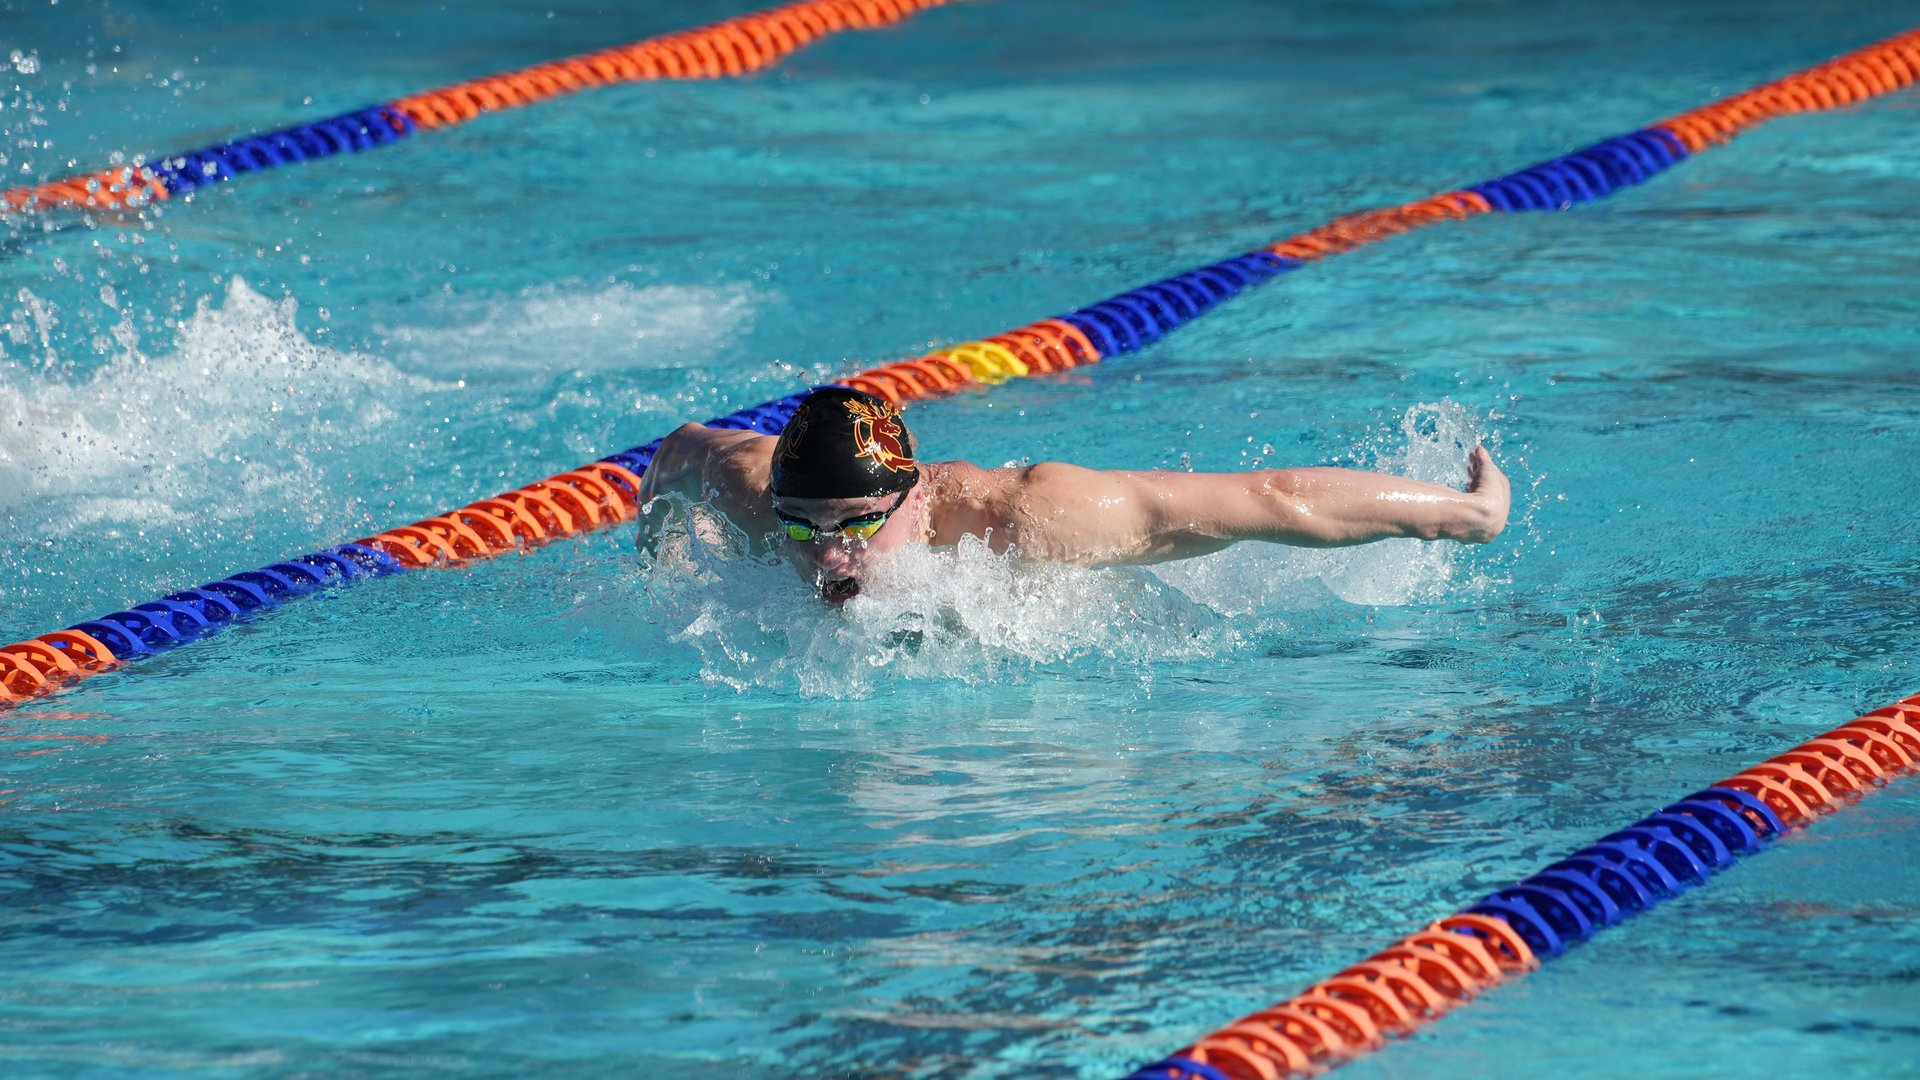
\includegraphics[width=0.6\textwidth, height=0.5\textheight, keepaspectratio]{../assets/highlights/Highlights/Headley0429.jpg}
    };
\end{tikzpicture}

\vfill
\end{center}
\clearpage
% Table Group 1: 50 Free + 100 Free
\begin{table}[H]
\centering
\begin{minipage}[t]{0.48\textwidth}
\centering
\textbf{50 Free}\\[0.1cm]
\begin{tabular}{@{}p{2.8cm}p{1.2cm}@{}}
\hline
    \textbf{NAME} & \textbf{YEAR} \\
\hline
    Mike TolFree & 1990 \\
    Steven Brende & 1998 \\
    Steven Brende & 1999 \\
    Eric Jones & 1969 \\
    Andrew Cox & 2005 \\
    Alan Diercks & 1988 \\
    Eric Jones & 1971 \\
    Bill Johnson & 1986 \\
    Bill Johnson & 1983 \\
    Bill Johnson & 1982 \\
    Erik Jensen & 1987 \\
    Ryan Carpenter & 2003 \\
    Dave Seidner & 1984 \\
    Nic Tekieli & 2022 \\
    Andrew Cosentino & 2008 \\
    Marco Conati & 2019 \\
    Eric Jones & 1970 \\
    Kris Behrens & 1997 \\
\hline
\end{tabular}
\end{minipage}\hfill
\begin{minipage}[t]{0.48\textwidth}
\centering
\textbf{100 Free}\\[0.1cm]
\begin{tabular}{@{}p{2.8cm}p{1.2cm}@{}}
\hline
    \textbf{NAME} & \textbf{YEAR} \\
\hline
    Eric Jones & 1970 \\
    Erik Jensen & 1987 \\
    Mike TolFree & 1990 \\
    David Brende & 1996 \\
    David Brende & 1995 \\
    Erik Jensen & 1989 \\
    Steven Brende & 1999 \\
    Ryan Carpenter & 2003 \\
    Noah Deer & 2016 \\
    Kris Behrens & 1997 \\
    Andrew Cox & 2005 \\
    Graham Spurzem & 2017 \\
    Bill Johnson & 1986 \\
    Andrew Cosentino & 2008 \\
    Nic Tekieli & 2022 \\
    Eric Jones & 1971 \\
\hline
\end{tabular}
\end{minipage}
\end{table}

% Table Group 2: 200 Free
\begin{table}[H]
\centering
\begin{minipage}[t]{0.6\textwidth}
\centering
\textbf{200 Free}\\[0.1cm]
\begin{tabular}{@{}p{2.8cm}p{1.2cm}@{}}
\hline
    \textbf{NAME} & \textbf{YEAR} \\
\hline
    Brent Davis & 1989 \\
    Steven Brende & 1999 \\
    Chris Derr & 1994 \\
    Doug Jones & 1982 \\
    David Brende & 1995 \\
    Andrew Cosentino & 2008 \\
    David Brende & 1997 \\
    Andrew Cox & 2005 \\
    David Brende & 1996 \\
    Scott Campbell & 1966 \\
    Anderson Breazeale & 2022 \\
\hline
\end{tabular}
\end{minipage}
\end{table}

% Table Group 3: 500 Free + 1650 Free
\begin{table}[H]
\centering
\begin{minipage}[t]{0.48\textwidth}
\centering
\textbf{500 Free}\\[0.1cm]
\begin{tabular}{@{}p{2.8cm}p{1.2cm}@{}}
\hline
    \textbf{NAME} & \textbf{YEAR} \\
\hline
    Chris Lloyd & 2000 \\
    Chris Lloyd & 1998 \\
    Mike Thornton & 1971 \\
    Marc Blumberg & 2013 \\
    Marc Blumberg & 2014 \\
    Chris Lloyd & 1999 \\
    Louis Caron & 1979 \\
    Marc Blumberg & 2012 \\
    Herbert Bowman & 1977 \\
    Scott Campbell & 1966 \\
    Paul Daigle & 1992 \\
    Paul Daigle & 1989 \\
    Doug Jones & 1982 \\
    Lucas Lang & 2022 \\
    David Brende & 1996 \\
    David Brende & 1995 \\
    Paul Daigle & 1990 \\
    Don Kuhn & 1987 \\
    David Brende & 1997 \\
    Doug Jones & 1983 \\
    Anderson Breazeale & 2024 \\
    David Kent & 1976 \\
    Chris Derr & 1994 \\
    Pat Culberson & 2017 \\
    Don Kuhn & 1985 \\
\hline
\end{tabular}
\end{minipage}\hfill
\begin{minipage}[t]{0.48\textwidth}
\centering
\textbf{1650 Free}\\[0.1cm]
\begin{tabular}{@{}p{2.8cm}p{1.2cm}@{}}
\hline
    \textbf{NAME} & \textbf{YEAR} \\
\hline
    Mike Thornton & 1971 \\
    Don Kuhn & 1985 \\
    Todd Thomas & 1989 \\
    Chris Lloyd & 1999 \\
    Lucas Lang & 2022 \\
    John Gudman & 1975 \\
    John Gudman & 1976 \\
    Lucas Lang & 2023 \\
    Lucas Lang & 2024 \\
    Chris Lloyd & 1998 \\
    Chris Lloyd & 2000 \\
    Mike Daigle & 1990 \\
    Alex Johnston & 1967 \\
    Conrad Shabb & 2013 \\
    Todd Thomas & 1988 \\
    Herbert Bowman & 1977 \\
    Ed Smith & 1986 \\
    Brett Berger & 2012 \\
    Conrad Shabb & 2014 \\
    Chris Derr & 1997 \\
\hline
\end{tabular}
\end{minipage}
\end{table}

% Table Group 4: 100 Back + 200 Back
\begin{table}[H]
\centering
\begin{minipage}[t]{0.48\textwidth}
\centering
\textbf{100 Back}\\[0.1cm]
\begin{tabular}{@{}p{2.8cm}p{1.2cm}@{}}
\hline
    \textbf{NAME} & \textbf{YEAR} \\
\hline
    Dave Seidner & 1984 \\
    Nic Tekieli & 2023 \\
    Ryan Beauregard & 1996 \\
    Tim Stallard & 1993 \\
    Nic Tekieli & 2022 \\
    Jon Schild & 1995 \\
    Doug Jones & 1983 \\
    Ryan Beauregard & 1998 \\
    Ryan Beauregard & 1997 \\
\hline
\end{tabular}
\end{minipage}\hfill
\begin{minipage}[t]{0.48\textwidth}
\centering
\textbf{200 Back}\\[0.1cm]
\begin{tabular}{@{}p{2.8cm}p{1.2cm}@{}}
\hline
    \textbf{NAME} & \textbf{YEAR} \\
\hline
    Bo Schoenfeld & 1972 \\
    Doug Jones & 1983 \\
    Doug Jones & 1982 \\
    Anderson Breazeale & 2024 \\
    Anderson Breazeale & 2023 \\
    Anderson Breazeale & 2022 \\
    Bo Schoenfeld & 1975 \\
    David Kent & 1976 \\
    David Kent & 1977 \\
    Scott Lichtig & 1973 \\
    Ryan Beauregard & 1995 \\
    Paul Daigle & 1992 \\
    Ryan Beauregard & 1996 \\
    Ryan Beauregard & 1997 \\
    Ryan Beauregard & 1998 \\
\hline
\end{tabular}
\end{minipage}
\end{table}

% Table Group 5: 100 Breast + 200 Breast
\begin{table}[H]
\centering
\begin{minipage}[t]{0.48\textwidth}
\centering
\textbf{100 Breast}\\[0.1cm]
\begin{tabular}{@{}p{2.8cm}p{1.2cm}@{}}
\hline
    \textbf{NAME} & \textbf{YEAR} \\
\hline
    Ryan Teeples & 1990 \\
    Nick Bagatelos & 1984 \\
    Nick Bagatelos & 1985 \\
    Mike Sutton & 1976 \\
    Evan Deedy & 2023 \\
    Ryan Teeples & 1989 \\
    Yoel Kende & 1975 \\
    Bill Johnson & 1986 \\
    Evan Deedy & 2024 \\
    Chris Faure & 1987 \\
    Gary Simon & 1998 \\
    Scott Cohen & 1991 \\
    Gary Simon & 1997 \\
    Scott Cohen & 1992 \\
\hline
\end{tabular}
\end{minipage}\hfill
\begin{minipage}[t]{0.48\textwidth}
\centering
\textbf{200 Breast}\\[0.1cm]
\begin{tabular}{@{}p{2.8cm}p{1.2cm}@{}}
\hline
    \textbf{NAME} & \textbf{YEAR} \\
\hline
    Jon Grinder & 1977 \\
    Ryan Teeples & 1991 \\
    Karl Graeber & 1969 \\
    Karl Graeber & 1968 \\
    Aaron Lutzker & 2016 \\
    Nick Bagatelos & 1985 \\
    Nick Bagatelos & 1984 \\
    Gary Simon & 1998 \\
    Karl Graeber & 1967 \\
    Richard Esterkin & 1973 \\
    Jon Grinder & 1979 \\
    Ned Busch & 1986 \\
    Kris Jurka & 2000 \\
    Ryan Teeples & 1990 \\
    Ryan Teeples & 1989 \\
    Gary Simon & 1997 \\
    Ryan Teeples & 1988 \\
    Mike Sutton & 1976 \\
\hline
\end{tabular}
\end{minipage}
\end{table}

% Table Group 6: 100 Fly + 200 Fly
\begin{table}[H]
\centering
\begin{minipage}[t]{0.48\textwidth}
\centering
\textbf{100 Fly}\\[0.1cm]
\begin{tabular}{@{}p{2.8cm}p{1.2cm}@{}}
\hline
    \textbf{NAME} & \textbf{YEAR} \\
\hline
    Patrick Shultz & 2014 \\
    Ryan Carpenter & 2004 \\
    Dave Lewis & 1985 \\
    Mike Eberhardt & 1996 \\
    Marco Conati & 2022 \\
    Mike Karcis & 1979 \\
    Patrick Shultz & 2015 \\
    Marco Conati & 2019 \\
    Erik Jensen & 1988 \\
    Brad Durbin & 1997 \\
    Frank Applebaum & 2023 \\
    Erik Jensen & 1987 \\
    Austin Hallett & 2010 \\
    Marco Conati & 2020 \\
    Frank Applebaum & 2024 \\
\hline
\end{tabular}
\end{minipage}\hfill
\begin{minipage}[t]{0.48\textwidth}
\centering
\textbf{200 Fly}\\[0.1cm]
\begin{tabular}{@{}p{2.8cm}p{1.2cm}@{}}
\hline
    \textbf{NAME} & \textbf{YEAR} \\
\hline
    David Tempkin & 1969 \\
    Jordan Lieberman & 2011 \\
    Dave Lewis & 1987 \\
    John Everett & 2017 \\
    Frank Applebaum & 2024 \\
    Frank Applebaum & 2023 \\
    Frank Applebaum & 2022 \\
    Mike Eberhardt & 1996 \\
    Paul Davis & 1989 \\
    Brent Davis & 1990 \\
    Mike Karcis & 1979 \\
\hline
\end{tabular}
\end{minipage}
\end{table}

% Table Group 7: 200 IM + 400 IM
\begin{table}[H]
\centering
\begin{minipage}[t]{0.48\textwidth}
\centering
\textbf{200 IM}\\[0.1cm]
\begin{tabular}{@{}p{2.8cm}p{1.2cm}@{}}
\hline
    \textbf{NAME} & \textbf{YEAR} \\
\hline
    Frank Applebaum & 2023 \\
    Brett Borisoff & 1973 \\
    Aaron Lutzker & 2017 \\
    David Tempkin & 1970 \\
    Takeshi Kaneko & 1995 \\
    Joe Busch & 1967 \\
    Joe Busch & 1969 \\
    Gary Simon & 1998 \\
    Mike Karcis & 1979 \\
    Ryan Teeples & 1991 \\
    Gary Simon & 1997 \\
    Ryan Teeples & 1990 \\
    Erik Jensen & 1989 \\
    Ryan Teeples & 1988 \\
    Frank Applebaum & 2022 \\
    Frank Applebaum & 2024 \\
\hline
\end{tabular}
\end{minipage}\hfill
\begin{minipage}[t]{0.48\textwidth}
\centering
\textbf{400 IM}\\[0.1cm]
\begin{tabular}{@{}p{2.8cm}p{1.2cm}@{}}
\hline
    \textbf{NAME} & \textbf{YEAR} \\
\hline
    Andrew Crowley & 2002 \\
    Conrad Shabb & 2014 \\
    Conrad Shabb & 2013 \\
    Ryan Teeples & 1991 \\
    John Mann & 1980 \\
    Chris Lloyd & 2001 \\
    Austin Hallett & 2009 \\
    Kris Jurka & 1997 \\
    Takeshi Kaneko & 1995 \\
    Henry Limm & 2017 \\
    Chris Lloyd & 1998 \\
    Chris Lloyd & 1999 \\
    Chris Lloyd & 2000 \\
    Matt Gannon & 2007 \\
    Paul Daigle & 1992 \\
    Paul Daigle & 1990 \\
    Garrett Martin & 1989 \\
\hline
\end{tabular}
\end{minipage}
\end{table}

% Table Group 8: 1-Meter
\begin{table}[H]
\centering
\begin{minipage}[t]{0.6\textwidth}
\centering
\textbf{1-Meter}\\[0.1cm]
\begin{tabular}{@{}p{2.8cm}p{1.2cm}@{}}
\hline
    \textbf{NAME} & \textbf{YEAR} \\
\hline
    Derek Eberhart & 1986 \\
    Derek Eberhart & 1985 \\
    Jack Griffith & 2023 \\
    G Dorst & 1977 \\
    Derek Eberhart & 1984 \\
    Mark Emanuel & 2006 \\
    Andrew Fevery & 2010 \\
    James Stevick & 2013 \\
    James Stevick & 2014 \\
    James Stevick & 2015 \\
    Ben Curtis & 1979 \\
    Cyrus Gaylord & 2024 \\
\hline
\end{tabular}
\end{minipage}
\end{table}

% Table Group 9: 3-Meter
\begin{table}[H]
\centering
\begin{minipage}[t]{0.6\textwidth}
\centering
\textbf{3-Meter}\\[0.1cm]
\begin{tabular}{@{}p{2.8cm}p{1.2cm}@{}}
\hline
    \textbf{NAME} & \textbf{YEAR} \\
\hline
    Mike Curtis & 1979 \\
    James Stevick & 2013 \\
    James Stevick & 2014 \\
    James Stevick & 2015 \\
    James Stevick & 2012 \\
    Derek Eberhart & 1984 \\
    Andrew Fevery & 2010 \\
    Derek Eberhart & 1986 \\
    Andrew Fevery & 2011 \\
    Derek Eberhart & 1985 \\
\hline
\end{tabular}
\end{minipage}
\end{table}

% ===== END CMS SCIAC Champions - Stag =====

\newpage

% ===== SCIAC All Time Top 10 Performers - Athena =====


\subsection{SCIAC All Time Top 10 Performers}

\newpage
\thispagestyle{empty}
\begin{center}
\vspace*{1cm}

% Title section at the top
\begin{tikzpicture}[overlay, remember picture]
    % Semi-transparent background for text
    \fill[white, opacity=0.9] ($(current page.north) + (-6cm, -2cm)$) rectangle ($(current page.north) + (6cm, -6cm)$);
    
    % Section title
    \node[anchor=center, text width=12cm, align=center] at ($(current page.north) + (0, -3.5cm)$) {
        \fontsize{36pt}{40pt}\selectfont\textbf{\textcolor{teamprimary}{SCIAC All Time Top 10 Performers}}
    };
    
    % Subsection title
    \node[anchor=center, text width=12cm, align=center] at ($(current page.north) + (0, -4.5cm)$) {
        \fontsize{24pt}{28pt}\selectfont\textbf{\textcolor{teamsecondary}{Athenas}}
    };
\end{tikzpicture}

% Image below the title
\vspace*{4cm}
\begin{tikzpicture}[overlay, remember picture]
    \node[anchor=center] at ($(current page.center) + (0, -1cm)$) {
        
\includegraphics[width=0.6\textwidth, height=0.5\textheight, keepaspectratio]{../assets/highlights/Highlights/DSC06244.jpg}
    };
\end{tikzpicture}

\vfill
\end{center}
\clearpage
% Table Group 1: 50 Free + 100 Free
% Table Group 1: 50 Free + 100 Free
\begin{table}[H]
    \centering
    \begin{minipage}[t]{0.48\textwidth}
    \centering
    \teamrecordtablewithteam{50 Free}{
        22.58 & Alex Turvey & 2024 & PP \\
        22.84 & Francesca Coppo & 2025 & PP \\
        23.00 & Avery Turney & 2022 & PP \\
        23.11 & Madison Kauahi & 2018 & PP \\
        23.21 & Alex Gill & 2023 & PP \\
        22.90 & Valerie Mello & 2025 & PP \\
        23.31 & Ava Sealander & 2022 & CMS \\
        23.31 & Chandra Lukes & 2013 & UR \\
        23.39 & Hannah Zurmuhl & 2019 & PP \\
        23.39 & Madeleine Kan & 2025 & CMS \\
        23.29 & Jocelyn Crawford & 2019 & CMS \\
    }
    \end{minipage}\hfill
    \begin{minipage}[t]{0.48\textwidth}
    \centering
    \teamrecordtablewithteam{100 Free}{
        51.23 & Chesna Pelka & 2024 & PP \\
        51.06 & Sabrina Wang & 2024 & PP \\
        51.05 & Kelly Ngo & 2016 & CMS \\
        50.77 & Madison Kauahi & 2017 & PP \\
        50.43 & Francesca Coppo & 2025 & PP \\
        50.38 & Nina Aballea & 2025 & PP \\
        49.56 & Alex Turvey & 2024 & PP \\
        50.10 & Avery Turney & 2022 & PP \\
        49.50 & Valerie Mello & 2025 & PP \\
        50.22 & Chandra Lukes & 2013 & UR \\
    }
    \end{minipage}
    \end{table}
    
    % Table Group 2: 200 Free + 500 Free
    \begin{table}[H]
    \centering
    \begin{minipage}[t]{0.48\textwidth}
    \centering
    \teamrecordtablewithteam{200 Free}{
        1:51.55 & Allie Bollella & 2010 & UR \\
        1:49.78 & Val Mello & 2025 & PP \\
        1:49.92 & Alex Turvey & 2023 & PP \\
        1:50.03 & Avery Turney & 2022 & PP \\
        1:50.28 & Mardell Ramirez & 2018 & CLU \\
        1:50.30 & Ella Blake & 2022 & CMS \\
        1:50.82 & Karolina Dzieciol & 2025 & PP \\
        1:51.13 & Charlotte Dixon & 2025 & PP \\
        1:51.44 & Maren Rusk & 2025 & PP \\
        1:51.68 & Brittany Percin & 2018 & CIT \\
    }
    \end{minipage}\hfill
    \begin{minipage}[t]{0.48\textwidth}
    \centering
    \teamrecordtablewithteam{500 Free}{
        4:59.91 & Christen Parker & 2001 & PP \\
        4:59.78 & Leila El Masri & 2022 & CMS \\
        4:57.37 & Katy Shaw & 2024 & CMS \\
        4:59.22 & Ella Blake & 2022 & CMS \\
        4:57.37 & Mia Syme & 2018 & CMS \\
        4:58.11 & Corley Smith & 2024 & CMS \\
        4:57.52 & Mardell Ramirez & 2018 & CLU \\
        5:00.00 & Kelsey Thomas & 2015 & PP \\
        4:58.57 & Abby Raclaw & 2024 & PP \\
        5:00.06 & Whitney Dawson & 2009 & CMS \\
    }
    \end{minipage}
    \end{table}
    
    % Table Group 3: 1650 Free + 100 Back
    \begin{table}[H]
    \centering
    \begin{minipage}[t]{0.48\textwidth}
    \centering
    \teamrecordtablewithteam{1650 Free}{
        17:09.09 & Lauren Williams & 1998 & CMS \\
        17:12.46 & Ella Blake & 2022 & CMS \\
        17:12.18 & Gracey Hiebert & 2020 & CMS \\
        17:11.27 & Bennett Jones & 2024 & PP \\
        17:09.26 & Lizzie Carrade & 2017 & CMS \\
        17:06.78 & Carliann Brasher & 2009 & CMS \\
        17:03.35 & Katy Shaw & 2024 & CMS \\
        17:03.21 & Mia Syme & 2019 & CMS \\
        16:58.48 & Whitney Dawson & 2009 & CMS \\
        17:12.74 & Corley Smith & 2014 & CMS \\
    }
    \end{minipage}\hfill
    \begin{minipage}[t]{0.48\textwidth}
    \centering
    \teamrecordtablewithteam{100 Back}{
        55.66 & Kelly Ngo & 2015 & CMS \\
        55.51 & Sarah Jin & 2017 & PP \\
        56.11 & Katie Bilotti & 2010 & CMS \\
        54.73 & Madeline Lovrensky & 2015 & ULV \\
        55.15 & Angela Ling & 2019 & PP \\
        55.22 & Izzy Yoon & 2025 & PP \\
        55.57 & Jocelyn Crawford & 2017 & CMS \\
        55.91 & Jamee Mitchum & 2022 & CMS \\
        56.04 & Amaia Sherman & 2025 & PP \\
        55.98 & Brooke Geske & 2020 & WC \\
    }
    \end{minipage}
    \end{table}
    
    % (Repeat the same structure for Table Groups 4, 5, 6, 7, 8, 9)
    

% Table Group 4: 200 Back + 100 Breast
% Table Group 4: 200 Back + 100 Breast
\begin{table}[H]
    \centering
    \begin{minipage}[t]{0.48\textwidth}
    \centering
    \teamrecordtablewithteam{200 Back}{
        2:01.43 & Kelly Ngo & 2015 & CMS \\
        2:02.13 & Jocelyn Crawford & 2017 & CMS \\
        2:01.94 & Angela Ling & 2019 & PP \\
        2:01.41 & Sarah Jin & 2017 & PP \\
        2:01.35 & Angela Ling & 2021 & PP \\
        2:00.69 & Katie Bilotti & 2010 & CMS \\
        2:00.22 & Jocelyn Crawford & 2018 & CMS \\
        2:00.14 & Angela Ling & 2020 & PP \\
        1:59.88 & Izzy Yoon & 2025 & PP \\
        2:00.16 & Amaia Sherman & 2025 & PP \\
    }
    \end{minipage}\hfill
    \begin{minipage}[t]{0.48\textwidth}
    \centering
    \teamrecordtablewithteam{100 Breast}{
        1:04.61 & Melissa Condon & 2010 & UR \\
        1:03.83 & Molly Buckley & 2020 & PP \\
        1:03.59 & Sydney Rosenfeld & 2018 & CMS \\
        1:03.57 & Augusta Lewis & 2021 & CMS \\
        1:03.44 & Melissa Condon & 2011 & UR \\
        1:03.24 & Augusta Lewis & 2020 & CMS \\
        1:02.86 & Audrey Hu & 2023 & CMS \\
        1:02.81 & Emmie Appl & 2024 & PP \\
        1:02.74 & Augusta Lewis & 2019 & CMS \\
        1:02.71 & Melissa Condon & 2012 & UR \\
    }
    \end{minipage}
    \end{table}
    
    % Table Group 5: 200 Breast + 100 Fly
    \begin{table}[H]
    \centering
    \begin{minipage}[t]{0.48\textwidth}
    \centering
    \teamrecordtablewithteam{200 Breast}{
        2:19.66 & Sydney Rosenfeld & 2018 & CMS \\
        2:19.40 & Augusta Lewis & 2019 & CMS \\
        2:19.36 & Molly Buckley & 2021 & PP \\
        2:19.30 & Melissa Condon & 2011 & UR \\
        2:18.94 & Augusta Lewis & 2020 & CMS \\
        2:18.72 & Emmie Appl & 2024 & PP \\
        2:18.69 & Audrey Hu & 2023 & CMS \\
        2:18.60 & Melissa Condon & 2012 & UR \\
        2:18.54 & Augusta Lewis & 2021 & CMS \\
        2:17.22 & Melissa Condon & 2013 & UR \\
    }
    \end{minipage}\hfill
    \begin{minipage}[t]{0.48\textwidth}
    \centering
    \teamrecordtablewithteam{100 Fly}{
        56.24 & Katie Bilotti & 2011 & CMS \\
        56.16 & Abby Yonan & 2018 & CMS \\
        56.06 & Katie Bilotti & 2010 & CMS \\
        55.99 & Augusta Lewis & 2021 & CMS \\
        55.77 & Alex Gill & 2023 & PP \\
        55.63 & Izzy Doud & 2024 & CMS \\
        55.47 & Izzy Doud & 2023 & CMS \\
        55.27 & Katie Bilotti & 2012 & CMS \\
        55.14 & Alex Gill & 2024 & PP \\
        55.04 & Izzy Doud & 2024 & CMS \\
    }
    \end{minipage}
    \end{table}
    
    % Table Group 6: 200 Fly + 200 IM
    \begin{table}[H]
    \centering
    \begin{minipage}[t]{0.48\textwidth}
    \centering
    \teamrecordtablewithteam{200 Fly}{
        2:04.76 & Katie Bilotti & 2012 & CMS \\
        2:04.56 & Augusta Lewis & 2019 & CMS \\
        2:03.92 & Augusta Lewis & 2020 & CMS \\
        2:03.69 & Augusta Lewis & 2021 & CMS \\
        2:03.39 & Alex Gill & 2023 & PP \\
        2:03.26 & Alex Gill & 2024 & PP \\
        2:02.90 & Izzy Doud & 2024 & CMS \\
        2:02.83 & Alex Gill & 2022 & PP \\
        2:02.62 & Izzy Doud & 2023 & CMS \\
        2:01.98 & Izzy Doud & 2024 & CMS \\
    }
    \end{minipage}\hfill
    \begin{minipage}[t]{0.48\textwidth}
    \centering
    \teamrecordtablewithteam{200 IM}{
        2:08.12 & Augusta Lewis & 2019 & CMS \\
        2:07.85 & Augusta Lewis & 2020 & CMS \\
        2:07.71 & Karolina Dzieciol & 2021 & PP \\
        2:07.42 & Augusta Lewis & 2021 & CMS \\
        2:07.23 & Emmie Appl & 2022 & PP \\
        2:07.12 & Karolina Dzieciol & 2023 & PP \\
        2:07.01 & Bennett Jones & 2024 & PP \\
        2:06.85 & Augusta Lewis & 2020 & CMS \\
        2:06.53 & Emmie Appl & 2024 & PP \\
        2:06.34 & Augusta Lewis & 2021 & CMS \\
    }
    \end{minipage}
    \end{table}
    
    % Table Group 7: 400 IM + 1-Meter (from your original message)
    \begin{table}[H]
    \centering
    \begin{minipage}[t]{0.48\textwidth}
    \centering
    \teamrecordtablewithteam{400 IM}{
        4:31.17 & Augusta Lewis & 2018 & CMS \\
        4:24.74 & Augusta Lewis & 2019 & CMS \\
        4:25.86 & Emmie Appl & 2022 & PP \\
        4:27.03 & Bennett Jones & 2023 & PP \\
        4:29.54 & Karolina Dzieciol & 2021 & PP \\
        4:30.03 & Allyson Yao & 2023 & CMS \\
        4:30.49 & Emmie Appl & 2024 & PP \\
        4:30.82 & Graeleigh Jones & 2022 & PP \\
        4:21.91 & Augusta Lewis & 2021 & CMS \\
        4:31.43 & Karolina Dzieciol & 2023 & PP \\
    }
    \end{minipage}\hfill
    \begin{minipage}[t]{0.48\textwidth}
    \centering
    \teamrecordtablewithteam{1-Meter}{
        268.86 & Jacque Desmond & 2018 & CMS \\
        265.50 & Ruby Epstein & 2019 & PP \\
        269.05 & Maia Presti/Carli Lessard & 2015/2017 & CMS \\
        267.00 & Alexis Romero & 2023 & CMS \\
        271.65 & Izzy Doud & 2024 & CMS \\
        263.65 & Mary Lynn Clark & 2017 & CMS \\
        294.30 & Ruby Epstein & 2021 & PP \\
        295.15 & Emma Ng Pack & 2021 & CMS \\
        310.55 & Maia Presti & 2017 & CMS \\
        273.15 & Eleanor Mackey & 2021 & PP \\
    }
    \end{minipage}
    \end{table}
    
    % Table Group 8: 3-Meter (single column)
    \begin{table}[H]
    \centering
    \teamrecordtablewithteam{3-Meter}{
        267.65 & Ruby Epstein & 2019 & PP \\
        279.60 & Maia Presti & 2017 & CMS \\
        289.85 & Ruby Epstein & 2021 & PP \\
        286.55 & Emma Ng Pack & 2021 & CMS \\
        297.50 & Maia Presti & 2017 & CMS \\
        287.05 & Alexis Romero & 2023 & CMS \\
        292.05 & Emma Ng Pack & 2022 & CMS \\
        280.15 & Maia Presti & 2015 & CMS \\
        273.75 & Emma Ng Pack & 2023 & CMS \\
        267.85 & Mary Lynn Clark & 2017 & CMS \\
    }
    \end{table}
    

% ===== END SCIAC All Time Top 10 Performers - Athena =====

\newpage

% ===== SCIAC All Time Top 10 Performers - Stag =====


\newpage
\thispagestyle{empty}
\begin{center}
\vspace*{1cm}

% Title section at the top
\begin{tikzpicture}[overlay, remember picture]
    % Semi-transparent background for text
    \fill[white, opacity=0.9] ($(current page.north) + (-6cm, -2cm)$) rectangle ($(current page.north) + (6cm, -6cm)$);
    
    % Section title
    \node[anchor=center, text width=12cm, align=center] at ($(current page.north) + (0, -3.5cm)$) {
        \fontsize{36pt}{40pt}\selectfont\textbf{\textcolor{teamprimary}{SCIAC All Time Top 10 Performers}}
    };
    
    % Subsection title
    \node[anchor=center, text width=12cm, align=center] at ($(current page.north) + (0, -4.5cm)$) {
        \fontsize{24pt}{28pt}\selectfont\textbf{\textcolor{teamsecondary}{Stags}}
    };
\end{tikzpicture}

% Image below the title
\vspace*{4cm}
\begin{tikzpicture}[overlay, remember picture]
    \node[anchor=center] at ($(current page.center) + (0, -1cm)$) {
        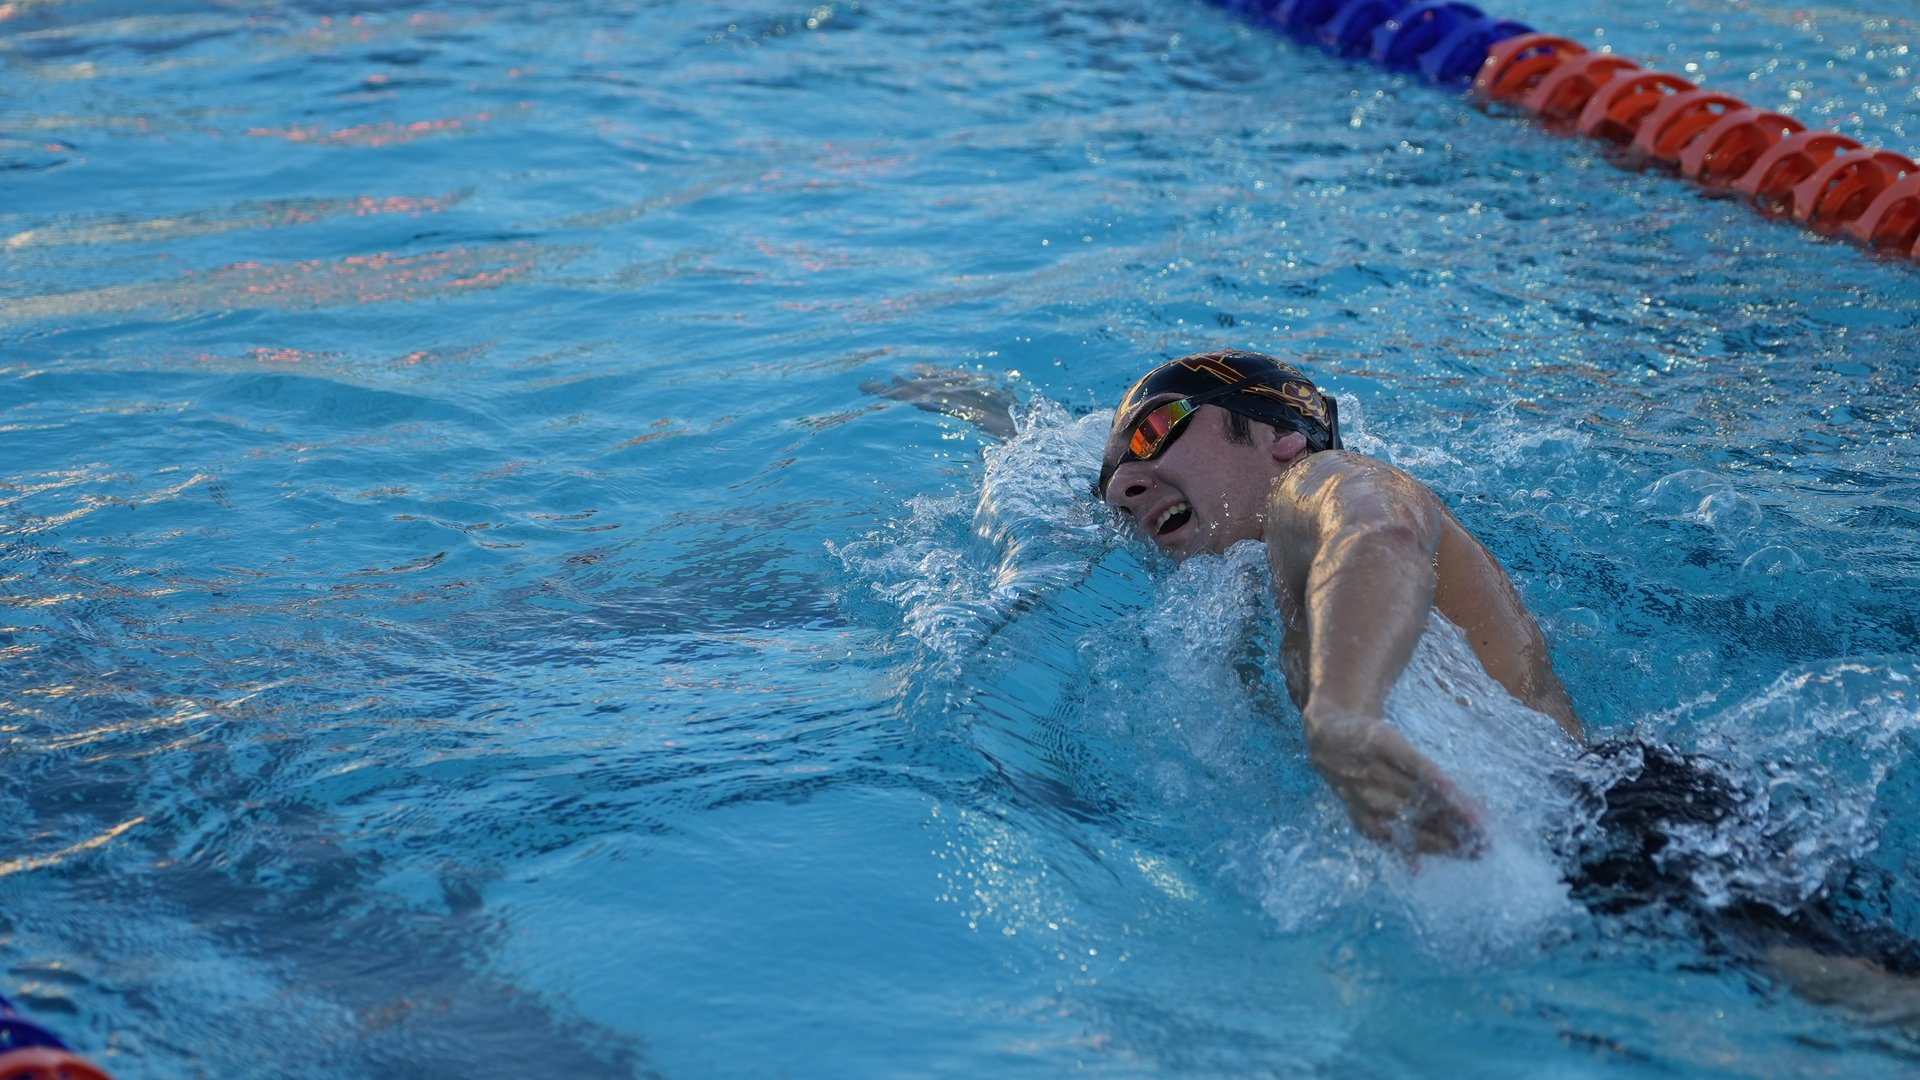
\includegraphics[width=0.6\textwidth, height=0.5\textheight, keepaspectratio]{../assets/highlights/Highlights/Gallegos9275.jpg}
    };
\end{tikzpicture}

\vfill
\end{center}
\clearpage
% Table Group 1: 50 Free + 100 Free
% Table Group 1: 50 Free + 100 Free
\begin{table}[H]
    \centering
    \begin{minipage}[t]{0.48\textwidth}
    \centering
    \teamrecordtablewithteam{50 Free}{
    19.98 & Nic Tekieli & 2022 & CMS \\
    19.74 & Casey Jacobs & 2025 & PP \\
    20.38 & Dylan Krueger & 2025 & CMS \\
    20.36 & Marco Conati & 2022 & CMS \\
    20.41 & Simon Jacobs & 2025 & CU \\
    20.39 & Tyler Harp & 2009 & UR \\
    20.30 & Cole Kershner & 2024 & CU \\
    20.22 & Andrew Cox & 2005 & CMS \\
    20.21 & Alex Poltash & 2015 & CMS \\
    20.31 & Miran Tirzic & 2009 & UR \\
    }
    \end{minipage}\hfill
    \begin{minipage}[t]{0.48\textwidth}
    \centering
    \teamrecordtablewithteam{100 Free}{
    44.06 & Alex Poltash & 2015 & CMS \\
    44.17 & Lukas Menkhoff & 2018 & PP \\
    44.21 & Marco Conati & 2022 & CMS \\
    44.54 & Simon Jacobs & 2025 & CU \\
    44.54 & Casey Jacobs & 2025 & PP \\
    44.60 & Tyler Harp & 2012 & UR \\
    44.73 & Nic Tekieli & 2022 & CMS \\
    44.73 & Mark Hallman & 2018 & PP \\
    44.94 & Noah Deer & 2016 & CMS \\
    44.76 & Tag Curwen & 2024 & PP \\
    }
    \end{minipage}
    \end{table}
    
    % Table Group 2: 200 Free + 500 Free
    \begin{table}[H]
    \centering
    \begin{minipage}[t]{0.48\textwidth}
    \centering
    \teamrecordtablewithteam{200 Free}{
    1:38.90 & Will Abele & 2019 & PP \\
    1:39.07 & Alex Poltash & 2015 & CMS \\
    1:39.08 & Adrian Clement & 2024 & PP \\
    1:39.14 & Cameron Whiting & 2015 & CMS \\
    1:38.20 & Mark Hallman & 2018 & PP \\
    1:37.54 & Tag Curwen & 2022 & PP \\
    1:37.51 & Tyler Harp & 2012 & UR \\
    1:37.29 & Anderson Breazeale & 2024 & CMS \\
    1:38.64 & Larry Yu & 2024 & PP \\
    1:38.35 & Matt Williams & 2017 & CMS \\
    }
    \end{minipage}\hfill
    \begin{minipage}[t]{0.48\textwidth}
    \centering
    \teamrecordtablewithteam{500 Free}{
    4:29.55 & Thomas Langlois & 2025 & WC \\
    4:27.51 & Will Abele & 2020 & PP \\
    4:26.99 & Ben Brewer & 2018 & CLU \\
    4:26.79 & Paddy Baylis & 2020 & PP \\
    4:26.66 & Mark Hallman & 2018 & PP \\
    4:26.28 & Larry Yu & 2023 & PP \\
    4:24.75 & Anderson Brezeale & 2024 & CMS \\
    4:24.54 & Lucas Lang & 2025 & CMS \\
    4:28.11 & Cameron Whiting & 2015 & CMS \\
    4:28.89 & Ben Culberson & 2017 & CMS \\
    }
    \end{minipage}
    \end{table}
    
    % Table Group 3: 1650 Free + 100 Back
    \begin{table}[H]
    \centering
    \begin{minipage}[t]{0.48\textwidth}
    \centering
    \teamrecordtablewithteam{1650 Free}{
    15:37.87 & Larry Yu & 2022 & PP \\
    15:25.66 & Paddy Baylis & 2019 & PP \\
    15:28.26 & Ben Brewer & 2017 & CLU \\
    15:29.21 & Thomas Langlois & 2024 & WC \\
    15:32.19 & Ben Culberson & 2017 & CMS \\
    15:32.87 & Cole Weiderman & 2024 & CLU \\
    15:35.59 & Tom Jansen & 2023 & UR \\
    15:45.57 & Conrad Shabb & 2014 & CMS \\
    15:46.13 & Brandon Pon & 2019 & ULV \\
    15:17.24 & Lucas Lang & 2022 & CMS \\
    }
    \end{minipage}\hfill
    \begin{minipage}[t]{0.48\textwidth}
    \centering
    \teamrecordtablewithteam{100 Back}{
    46.99 & Nic Tekieli & 2022 & CMS \\
    48.76 & Frank Applebaum & 2024 & CMS \\
    48.64 & Larry Yu & 2024 & PP \\
    49.44 & Jeffrey Depew & 2012 & UR \\
    47.57 & Matt Williams & 2016 & CMS \\
    49.44 & Nikhil Kundu & 2019 & PP \\
    49.32 & Anderson Breazeale & 2020 & CMS \\
    49.07 & Samuel To & 2018 & PP \\
    48.43 & Jeremy Tan & 2025 & CMS \\
    49.55 & Garrett Krattiger & 2025 & UR \\
    }
    \end{minipage}
    \end{table}
    
    % Table Group 4: 200 Back + 100 Breast
    \begin{table}[H]
    \centering
    \begin{minipage}[t]{0.48\textwidth}
    \centering
    \teamrecordtablewithteam{200 Back}{
    1:46.51 & Anderson Breazeale & 2022 & CMS \\
    1:45.67 & Matt Williams & 2014 & CMS \\
    1:45.05 & Nic Tekieli & 2022 & CMS \\
    1:48.12 & Jeff Depew & 2013 & UR \\
    1:46.78 & Liam O'Shea & 2020 & PP \\
    1:47.46 & Diego Hodge & 2024 & PP \\
    1:47.65 & Garrett Krattiger & 2025 & UR \\
    1:47.66 & Jeremy Tan & 2025 & CMS \\
    1:48.04 & Larry Yu & 2024 & PP \\
    1:48.17 & Nick Jasinski & 2019 & CIT \\
    }
    \end{minipage}\hfill
    \begin{minipage}[t]{0.48\textwidth}
    \centering
    \teamrecordtablewithteam{100 Breast}{
    55.06 & Tom Gallup & 2017 & CIT \\
    55.11 & Jason Lin & 2022 & CIT \\
    54.91 & Tony Martir & 2016 & WC \\
    54.88 & Walter Limm & 2022 & CMS \\
    54.71 & S VanDeventer & 2015 & OXY \\
    52.71 & Luke Rodarte & 2022 & CLU \\
    53.39 & Lukas Menkhoff & 2018 & PP \\
    53.87 & Lincoln Hall & 2025 & CLU \\
    53.90 & Evan Deedy & 2025 & CMS \\
    54.29 & Larry Yu & 2024 & PP \\
    }
    \end{minipage}
    \end{table}
    
    % Table Group 5: 200 Breast + 100 Fly
    \begin{table}[H]
    \centering
    \begin{minipage}[t]{0.48\textwidth}
    \centering
    \teamrecordtablewithteam{200 Breast}{
    1:59.24 & Lincoln Hall & 2025 & CLU \\
    2:00.15 & Markus Stegbuchner & 2025 & CLU \\
    2:00.76 & Thomas Fenton & 2024 & CIT \\
    1:59.26 & Issac Pan & 2024 & PP \\
    1:58.86 & Evan Deedy & 2025 & CMS \\
    1:58.21 & S VanDeventer & 2014 & OXY \\
    1:58.05 & Larry Yu & 2023 & PP \\
    2:00.10 & Jason Lin & 2022 & CIT \\
    1:56.69 & Luke Rodarte & 2022 & CLU \\
    1:59.90 & Vincent Pai & 2009 & CMS \\
    }
    \end{minipage}\hfill
    \begin{minipage}[t]{0.48\textwidth}
    \centering
    \teamrecordtablewithteam{100 Fly}{
    48.60 & Ryan Drover & 2018 & PP \\
    48.51 & AJ Nybo & 2022 & CLU \\
    48.42 & Kyle Huang & 2024 & PP \\
    48.39 & Trenten Calloway & 2025 & CU \\
    47.71 & Zu Pigot & 2018 & WC \\
    47.88 & Austin Lashley & 2018 & OXY \\
    47.13 & Frank Applebaum & 2024 & CMS \\
    47.56 & Marco Conati & 2022 & CMS \\
    48.61 & Marcel Liu & 2024 & CIT \\
    47.80 & Matt Williams & 2017 & CMS \\
    }
    \end{minipage}
    \end{table}
    
    % Table Group 6: 200 Fly + 200 IM
    \begin{table}[H]
    \centering
    \begin{minipage}[t]{0.48\textwidth}
    \centering
    \teamrecordtablewithteam{200 Fly}{
    1:45.38 & Jeff Depew & 2014 & UR \\
    1:46.75 & Kyle Huang & 2025 & PP \\
    1:46.93 & AJ Nybo & 2022 & CLU \\
    1:47.72 & Pierre Zeineddin & 2022 & CIT \\
    1:48.11 & Chris Depew & 2013 & UR \\
    1:48.85 & Diego Hodge & 2025 & PP \\
    1:43.39 & Frank Applebaum & 2024 & CMS \\
    1:48.57 & Will Abele & 2020 & PP \\
    1:48.70 & Matt Valentine & 2016 & CMS \\
    1:48.71 & Gordon Kenny & 2024 & PP \\
    }
    \end{minipage}\hfill
    \begin{minipage}[t]{0.48\textwidth}
    \centering
    \teamrecordtablewithteam{200 IM}{
    1:48.96 & Issac Pan & 2024 & PP \\
    1:48.74 & Frank Applebaum & 2023 & CMS \\
    1:48.71 & AJ Nybo & 2020 & CLU \\
    1:48.55 & Collin Gladys & 2010 & UR \\
    1:46.38 & Frank Applebaum & 2024 & CMS \\
    1:46.97 & Gary Simon & 1998 & CMS \\
    1:47.06 & Jeffrey Depew & 2015 & UR \\
    1:48.40 & Chris Depew & 2013 & UR \\
    1:49.03 & Samuel To & 2016 & PP \\
    1:46.79 & Larry Yu & 2024 & PP \\
    }
    \end{minipage}
    \end{table}
    
    % Table Group 7: 400 IM
    \begin{table}[H]
    \centering
    \begin{minipage}[t]{0.6\textwidth}
    \centering
    \teamrecordtablewithteam{400 IM}{
    3:55.33 & Kyle Huang & 2024 & PP \\
    3:56.88 & Conrad Shabb & 2014 & CMS \\
    3:58.45 & Henrik Barck & 2024 & CMS \\
    3:55.61 & Henry Limm & 2018 & CMS \\
    3:56.68 & Tom Harrison & 1983 & CMS \\
    3:56.25 & Jason Lu & 2019 & PP \\
    3:51.96 & Jeff Depew & 2015 & UR \\
    3:52.09 & Larry Yu & 2023 & PP \\
    3:54.50 & Liam O'Shea & 2020 & PP \\
    3:54.52 & Chris Depew & 2013 & UR \\
    }
    \end{minipage}
    \end{table}
    
    % Table Group 8: 1-Meter (11 dives)
    \begin{table}[H]
    \centering
    \begin{minipage}[t]{0.6\textwidth}
    \centering
    \teamrecordtablewithteam{1-Meter (11 dives)}{
    507.50 & Sam Solomon & 2022 & CIT \\
    505.75 & Tyler Aisner & 2012 & WC \\
    499.35 & Patrick Quarberg & 2016 & CMS \\
    499.10 & Joey Luba & 2015 & CU \\
    498.40 & Scott MacKay & 2016 & ULV \\
    497.45 & Billy Altantulkhuur & 2018 & PP \\
    541.05 & Brian Forster & 1993 & PP \\
    594.05 & Kendall Hollimon & 2017 & CMS \\
    497.30 & Terry Thompson & 1980 & CIT \\
    628.60 & James Stevick & 2015 & CMS \\
    }
    \end{minipage}
    \end{table}
    
    % Table Group 9: 3-Meter (11 dives)
    \begin{table}[H]
    \centering
    \begin{minipage}[t]{0.6\textwidth}
    \centering
    \teamrecordtablewithteam{3-Meter (11 dives)}{
    524.80 & Robert Dohring & 2007 & OXY \\
    523.65 & Brian Forster & 1993 & PP \\
    524.00 & Tommy Matheis & 2025 & PP \\
    627.60 & James Stevick & 2015 & CMS \\
    624.50 & Kendall Hollimon & 2018 & CMS \\
    556.35 & Patrick Quarberg & 2015 & CMS \\
    538.25 & Jon Dohring & 2007 & OXY \\
    537.00 & Scott MacKay & 2015 & ULV \\
    529.40 & Ben Willett & 2023 & PP \\
    529.80 & Jem Stern & 2019 & PP \\
    }
    \end{minipage}
    \end{table}
    

% ===== END SCIAC All Time Top 10 Performers - Stag =====

\newpage

% ===== SCIAC Records - Women =====


\subsection{SCIAC Records}

\newpage
\thispagestyle{empty}
\begin{center}
\vspace*{1cm}

% Title section at the top
\begin{tikzpicture}[overlay, remember picture]
    % Semi-transparent background for text
    \fill[white, opacity=0.9] ($(current page.north) + (-6cm, -2cm)$) rectangle ($(current page.north) + (6cm, -6cm)$);
    
    % Section title
    \node[anchor=center, text width=12cm, align=center] at ($(current page.north) + (0, -3.5cm)$) {
        \fontsize{36pt}{40pt}\selectfont\textbf{\textcolor{teamprimary}{SCIAC Records}}
    };
    
    % Subsection title
    \node[anchor=center, text width=12cm, align=center] at ($(current page.north) + (0, -4.5cm)$) {
        \fontsize{24pt}{28pt}\selectfont\textbf{\textcolor{teamsecondary}{Women}}
    };
\end{tikzpicture}

% Image below the title
\vspace*{4cm}
\begin{tikzpicture}[overlay, remember picture]
    \node[anchor=center] at ($(current page.center) + (0, -1cm)$) {
        \includegraphics[width=0.6\textwidth, height=0.5\textheight, keepaspectratio]{../assets/highlights/Highlights/MSDSCIACs02225 (1).jpg}
    };
\end{tikzpicture}

\vfill
\end{center}
\clearpage
% Table Group 1: 50 Free + 100 Free
\begin{table}[H]
\centering
\begin{minipage}[t]{0.48\textwidth}
\centering
\textbf{50 Free}\\[0.1cm]
\begin{tabular}{@{}p{1.8cm}p{2.8cm}p{1.2cm}p{1.4cm}p{1.4cm}@{}}
\hline
    \textbf{TIME} & \textbf{NAME} & \textbf{YEAR} & \textbf{TEAM} & \textbf{MEET} \\
\hline
    22.58 & Alex Turvey & 2024 & PP & SCIAC \\
    22.84 & Francesca Coppo & 2025 & PP & Meet \\
\hline
\end{tabular}
\end{minipage}\hfill
\begin{minipage}[t]{0.48\textwidth}
\centering
\textbf{100 Free}\\[0.1cm]
\begin{tabular}{@{}p{1.8cm}p{2.8cm}p{1.2cm}p{1.4cm}p{1.4cm}@{}}
\hline
    \textbf{TIME} & \textbf{NAME} & \textbf{YEAR} & \textbf{TEAM} & \textbf{MEET} \\
\hline
    49.83 & Alex Turvey & 2024 & PP & Meet \\
    49.50 & Valerie Mello & 2025 & PP & SCIAC \\
\hline
\end{tabular}
\end{minipage}
\end{table}

% Table Group 2: 200 Free + 500 Free
\begin{table}[H]
\centering
\begin{minipage}[t]{0.48\textwidth}
\centering
\textbf{200 Free}\\[0.1cm]
\begin{tabular}{@{}p{1.8cm}p{2.8cm}p{1.2cm}p{1.4cm}p{1.4cm}@{}}
\hline
    \textbf{TIME} & \textbf{NAME} & \textbf{YEAR} & \textbf{TEAM} & \textbf{MEET} \\
\hline
    1:49.78 & Valerie Mello & 2025 & PP & Meet \\
    1:49.78 & Valerie Mello & 2025 & PP & SCIAC \\
\hline
\end{tabular}
\end{minipage}\hfill
\begin{minipage}[t]{0.48\textwidth}
\centering
\textbf{500 Free}\\[0.1cm]
\begin{tabular}{@{}p{1.8cm}p{2.8cm}p{1.2cm}p{1.4cm}p{1.4cm}@{}}
\hline
    \textbf{TIME} & \textbf{NAME} & \textbf{YEAR} & \textbf{TEAM} & \textbf{MEET} \\
\hline
    4:57.37 & Mia Syme/Katy Shaw & 2018/2024 & CMS & SCIAC \\
    4:57.37 & Mia Syme/Katy Shaw & 2018/2024 & CMS & Meet \\
\hline
\end{tabular}
\end{minipage}
\end{table}

% Table Group 3: 1650 Free + 100 Back
\begin{table}[H]
\centering
\begin{minipage}[t]{0.48\textwidth}
\centering
\textbf{1650 Free}\\[0.1cm]
\begin{tabular}{@{}p{1.8cm}p{2.8cm}p{1.2cm}p{1.4cm}p{1.4cm}@{}}
\hline
    \textbf{TIME} & \textbf{NAME} & \textbf{YEAR} & \textbf{TEAM} & \textbf{MEET} \\
\hline
    17:03.21 & Mia Syme & 2019 & CMS & Meet \\
    16:58.48 & Whitney Dawson & 2009 & CMS & SCIAC \\
\hline
\end{tabular}
\end{minipage}\hfill
\begin{minipage}[t]{0.48\textwidth}
\centering
\textbf{100 Back}\\[0.1cm]
\begin{tabular}{@{}p{1.8cm}p{2.8cm}p{1.2cm}p{1.4cm}p{1.4cm}@{}}
\hline
    \textbf{TIME} & \textbf{NAME} & \textbf{YEAR} & \textbf{TEAM} & \textbf{MEET} \\
\hline
    55.15 & Angela Ling & 2019 & PP & Meet \\
    54.73 & Maddie Lovrensky & 2015 & LaVerne & SCIAC \\
\hline
\end{tabular}
\end{minipage}
\end{table}

% Table Group 4: 200 Back + 100 Breast
\begin{table}[H]
\centering
\begin{minipage}[t]{0.48\textwidth}
\centering
\textbf{200 Back}\\[0.1cm]
\begin{tabular}{@{}p{1.8cm}p{2.8cm}p{1.2cm}p{1.4cm}p{1.4cm}@{}}
\hline
    \textbf{TIME} & \textbf{NAME} & \textbf{YEAR} & \textbf{TEAM} & \textbf{MEET} \\
\hline
    1:59.63 & Izzy Yoon & 2025 & PP & SCIAC \\
    2:00.61 & Izzy Yoon & 2025 & PP & Meet \\
\hline
\end{tabular}
\end{minipage}\hfill
\begin{minipage}[t]{0.48\textwidth}
\centering
\textbf{100 Breast}\\[0.1cm]
\begin{tabular}{@{}p{1.8cm}p{2.8cm}p{1.2cm}p{1.4cm}p{1.4cm}@{}}
\hline
    \textbf{TIME} & \textbf{NAME} & \textbf{YEAR} & \textbf{TEAM} & \textbf{MEET} \\
\hline
    1:01.59 & Alexandra Gill & 2023 & PP & Meet \\
    1:01.21 & Alexandra Gill & 2023 & PP & SCIAC \\
\hline
\end{tabular}
\end{minipage}
\end{table}

% Table Group 5: 200 Breast + 100 Fly
\begin{table}[H]
\centering
\begin{minipage}[t]{0.48\textwidth}
\centering
\textbf{200 Breast}\\[0.1cm]
\begin{tabular}{@{}p{1.8cm}p{2.8cm}p{1.2cm}p{1.4cm}p{1.4cm}@{}}
\hline
    \textbf{TIME} & \textbf{NAME} & \textbf{YEAR} & \textbf{TEAM} & \textbf{MEET} \\
\hline
    2:14.30 & Alexandra Gill & 2023 & PP & Meet \\
    2:14.30 & Alexandra Gill & 2023 & PP & SCIAC \\
\hline
\end{tabular}
\end{minipage}\hfill
\begin{minipage}[t]{0.48\textwidth}
\centering
\textbf{100 Fly}\\[0.1cm]
\begin{tabular}{@{}p{1.8cm}p{2.8cm}p{1.2cm}p{1.4cm}p{1.4cm}@{}}
\hline
    \textbf{TIME} & \textbf{NAME} & \textbf{YEAR} & \textbf{TEAM} & \textbf{MEET} \\
\hline
    53.76 & Alex Turvey & 2024 & PP & Meet \\
    53.57 & Alex Turvey & 2024 & PP & SCIAC \\
\hline
\end{tabular}
\end{minipage}
\end{table}

% Table Group 6: 200 Fly + 200 IM
\begin{table}[H]
\centering
\begin{minipage}[t]{0.48\textwidth}
\centering
\textbf{200 Fly}\\[0.1cm]
\begin{tabular}{@{}p{1.8cm}p{2.8cm}p{1.2cm}p{1.4cm}p{1.4cm}@{}}
\hline
    \textbf{TIME} & \textbf{NAME} & \textbf{YEAR} & \textbf{TEAM} & \textbf{MEET} \\
\hline
    2:01.30 & Mackenzie Mayfield & 2025 & CMS & Meet \\
    2:01.30 & Mackenzie Mayfield & 2025 & CMS & SCIAC \\
\hline
\end{tabular}
\end{minipage}\hfill
\begin{minipage}[t]{0.48\textwidth}
\centering
\textbf{200 IM}\\[0.1cm]
\begin{tabular}{@{}p{1.8cm}p{2.8cm}p{1.2cm}p{1.4cm}p{1.4cm}@{}}
\hline
    \textbf{TIME} & \textbf{NAME} & \textbf{YEAR} & \textbf{TEAM} & \textbf{MEET} \\
\hline
    2:00.69 & Augusta Lewis & 2023 & CMS & Meet \\
    2:00.69 & Augusta Lewis & 2023 & CMS & SCIAC \\
\hline
\end{tabular}
\end{minipage}
\end{table}

% Table Group 7: 400 IM
\begin{table}[H]
\centering
\begin{minipage}[t]{0.6\textwidth}
\centering
\textbf{400 IM}\\[0.1cm]
\begin{tabular}{@{}p{1.8cm}p{2.8cm}p{1.2cm}p{1.4cm}p{1.4cm}@{}}
\hline
    \textbf{TIME} & \textbf{NAME} & \textbf{YEAR} & \textbf{TEAM} & \textbf{MEET} \\
\hline
    4:18.66 & Augusta Lewis & 2022 & CMS & Meet \\
    4:15.73 & Augusta Lewis & 2023 & CMS & SCIAC \\
\hline
\end{tabular}
\end{minipage}
\end{table}

% Table Group 8: 1-Meter
\begin{table}[H]
\centering
\begin{minipage}[t]{0.6\textwidth}
\centering
\textbf{1-Meter}\\[0.1cm]
\begin{tabular}{@{}p{1.8cm}p{2.8cm}p{1.2cm}p{1.4cm}p{1.4cm}@{}}
\hline
    \textbf{TIME} & \textbf{NAME} & \textbf{YEAR} & \textbf{TEAM} & \textbf{MEET} \\
\hline
    525.35 & Maia Presti & 2015 & CMS & Meet \\
    525.35 & Maia Presti & 2015 & CMS & SCIAC \\
\hline
\end{tabular}
\end{minipage}
\end{table}

% Table Group 9: 3-Meter
\begin{table}[H]
\centering
\begin{minipage}[t]{0.6\textwidth}
\centering
\textbf{3-Meter}\\[0.1cm]
\begin{tabular}{@{}p{1.8cm}p{2.8cm}p{1.2cm}p{1.4cm}p{1.4cm}@{}}
\hline
    \textbf{TIME} & \textbf{NAME} & \textbf{YEAR} & \textbf{TEAM} & \textbf{MEET} \\
\hline
    491.85 & Jessica Robson & 2014 & Occidental & SCIAC \\
    491.85 & Jessica Robson & 2014 & Occidental & Meet \\
\hline
\end{tabular}
\end{minipage}
\end{table}

% Table Group 10: 200 Free Relay
\begin{table}[H]
\centering
\begin{minipage}[t]{0.6\textwidth}
\centering
\textbf{200 Free Relay}\\[0.1cm]
\begin{tabular}{@{}p{1.8cm}p{2.8cm}p{1.2cm}p{1.4cm}p{1.4cm}@{}}
\hline
    \textbf{TIME} & \textbf{NAME} & \textbf{YEAR} & \textbf{TEAM} & \textbf{MEET} \\
\hline
    1:32.05 & Lee, Coppo, Pelka, Mello & 2025 & PP & Meet \\
    1:31.48 & Coppo, Lee, Pelka, Mello & 2025 & PP & SCIAC \\
\hline
\end{tabular}
\end{minipage}
\end{table}

% Table Group 11: 400 Free Relay
\begin{table}[H]
\centering
\begin{minipage}[t]{0.6\textwidth}
\centering
\textbf{400 Free Relay}\\[0.1cm]
\begin{tabular}{@{}p{1.8cm}p{2.8cm}p{1.2cm}p{1.4cm}p{1.4cm}@{}}
\hline
    \textbf{TIME} & \textbf{NAME} & \textbf{YEAR} & \textbf{TEAM} & \textbf{MEET} \\
\hline
    3:21.54 & Coppo, Abellea, Dixon, Mello & 2025 & PP & Meet \\
    3:20.59 & Wang, Turvey, Gould, Mello & 2024 & PP & SCIAC \\
\hline
\end{tabular}
\end{minipage}
\end{table}

% Table Group 12: 800 Free Relay
\begin{table}[H]
\centering
\begin{minipage}[t]{0.6\textwidth}
\centering
\textbf{800 Free Relay}\\[0.1cm]
\begin{tabular}{@{}p{1.8cm}p{2.8cm}p{1.2cm}p{1.4cm}p{1.4cm}@{}}
\hline
    \textbf{TIME} & \textbf{NAME} & \textbf{YEAR} & \textbf{TEAM} & \textbf{MEET} \\
\hline
    7:24.79 & Wang, Turvey, Rusk, Gould & 2024 & PP & Meet \\
    7:23.87 & Dzieciol, Dixon, Rusk, Mello & 2025 & PP & SCIAC \\
\hline
\end{tabular}
\end{minipage}
\end{table}

% Table Group 13: 200 Medley Relay
\begin{table}[H]
\centering
\begin{minipage}[t]{0.6\textwidth}
\centering
\textbf{200 Medley Relay}\\[0.1cm]
\begin{tabular}{@{}p{1.8cm}p{2.8cm}p{1.2cm}p{1.4cm}p{1.4cm}@{}}
\hline
    \textbf{TIME} & \textbf{NAME} & \textbf{YEAR} & \textbf{TEAM} & \textbf{MEET} \\
\hline
    1:41.67 & Liao, Gill, Turvey, Gould & 2023 & PP & SCIAC \\
    1:41.67 & Liao, Gill, Turvey, Gould & 2023 & PP & Meet \\
\hline
\end{tabular}
\end{minipage}
\end{table}

% Table Group 14: 400 Medley Relay
\begin{table}[H]
\centering
\begin{minipage}[t]{0.6\textwidth}
\centering
\textbf{400 Medley Relay}\\[0.1cm]
\begin{tabular}{@{}p{1.8cm}p{2.8cm}p{1.2cm}p{1.4cm}p{1.4cm}@{}}
\hline
    \textbf{TIME} & \textbf{NAME} & \textbf{YEAR} & \textbf{TEAM} & \textbf{MEET} \\
\hline
    3:43.07 & Brooks, Gill, Turvey, Gould & 2023 & PP & SCIAC \\
    3:43.07 & Brooks, Gill, Turvey, Gould & 2023 & PP & Meet \\
\hline
\end{tabular}
\end{minipage}
\end{table}

% ===== END SCIAC Records - Women =====

\newpage

% ===== SCIAC Records - Men =====


\newpage
\thispagestyle{empty}
\begin{center}
\vspace*{1cm}

% Title section at the top
\begin{tikzpicture}[overlay, remember picture]
    % Semi-transparent background for text
    \fill[white, opacity=0.9] ($(current page.north) + (-6cm, -2cm)$) rectangle ($(current page.north) + (6cm, -6cm)$);
    
    % Section title
    \node[anchor=center, text width=12cm, align=center] at ($(current page.north) + (0, -3.5cm)$) {
        \fontsize{36pt}{40pt}\selectfont\textbf{\textcolor{teamprimary}{SCIAC Records}}
    };
    
    % Subsection title
    \node[anchor=center, text width=12cm, align=center] at ($(current page.north) + (0, -4.5cm)$) {
        \fontsize{24pt}{28pt}\selectfont\textbf{\textcolor{teamsecondary}{Men}}
    };
\end{tikzpicture}

% Image below the title
\vspace*{4cm}
\begin{tikzpicture}[overlay, remember picture]
    \node[anchor=center] at ($(current page.center) + (0, -1cm)$) {
        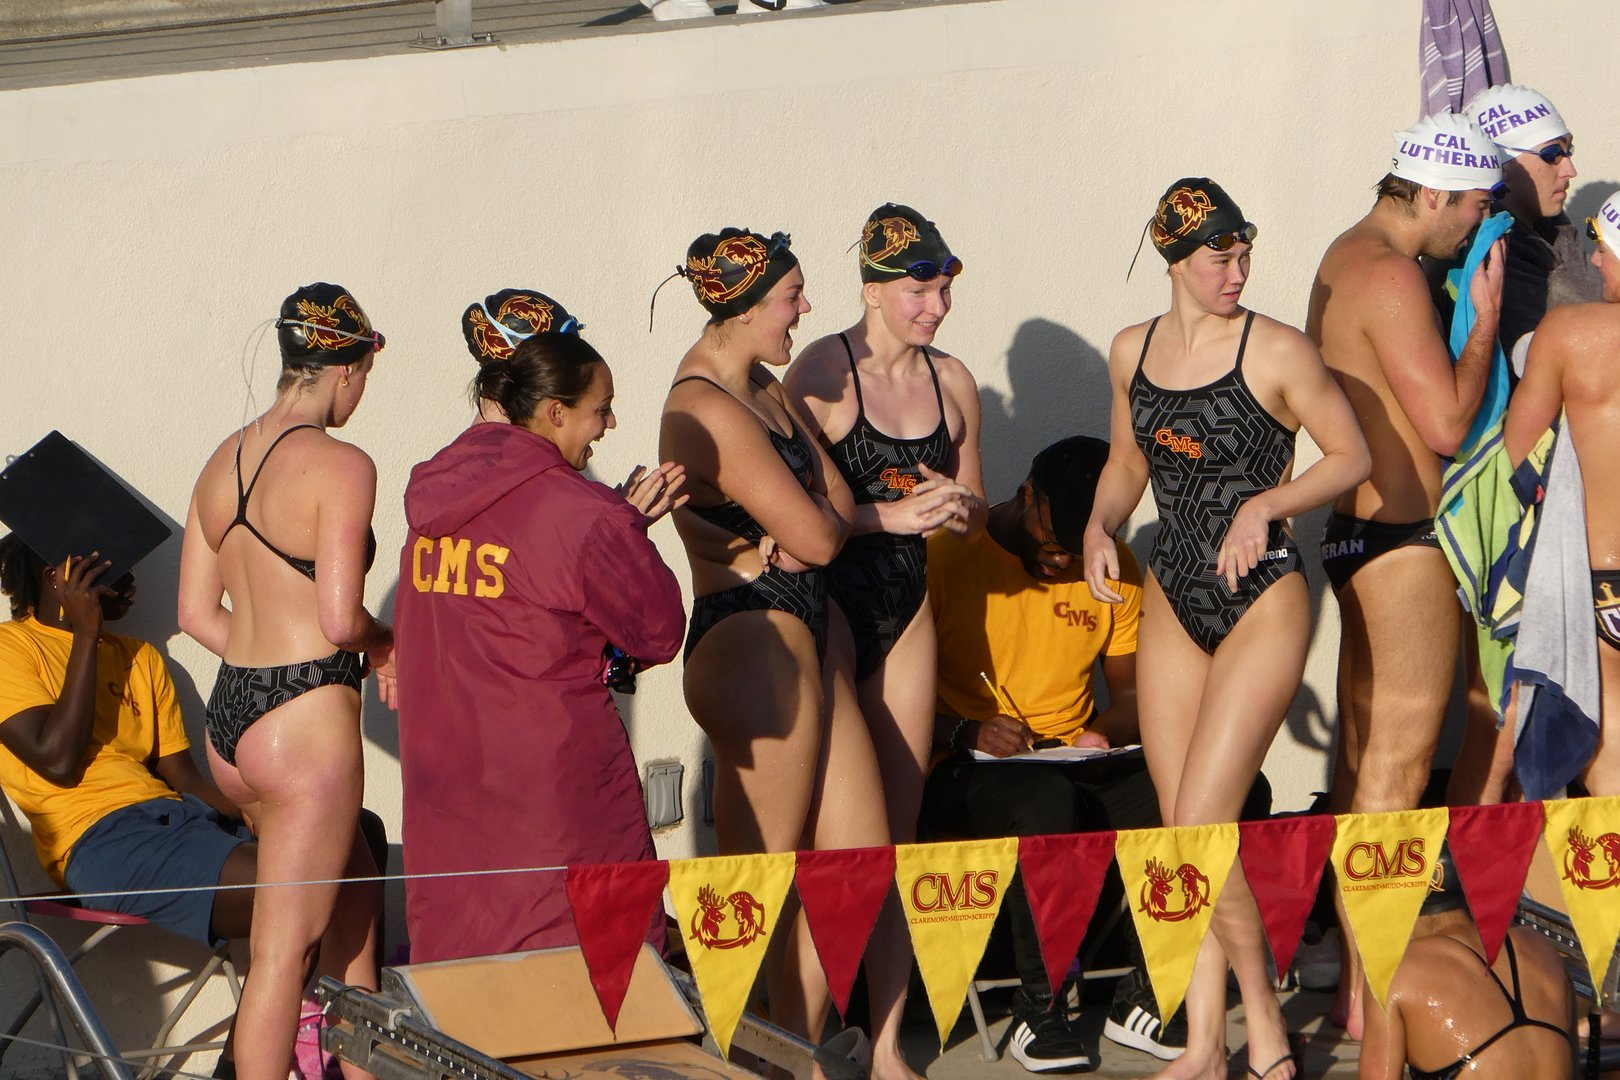
\includegraphics[width=0.6\textwidth, height=0.5\textheight, keepaspectratio]{../assets/highlights/Highlights/IMG_7533.jpg}
    };
\end{tikzpicture}

\vfill
\end{center}
\clearpage
% Table Group 1: 50 Free + 100 Free
\begin{table}[H]
\centering
\begin{minipage}[t]{0.48\textwidth}
\centering
\textbf{50 Free}\\[0.1cm]
\begin{tabular}{@{}p{1.8cm}p{2.8cm}p{1.2cm}p{1.4cm}p{1.4cm}@{}}
\hline
    \textbf{TIME} & \textbf{NAME} & \textbf{YEAR} & \textbf{TEAM} & \textbf{MEET} \\
\hline
    19.74 & Casey Jacobs & 2025 & PP & SCIAC \\
    20.14 & Casey Jacobs & 2025 & PP & Meet \\
\hline
\end{tabular}
\end{minipage}\hfill
\begin{minipage}[t]{0.48\textwidth}
\centering
\textbf{100 Free}\\[0.1cm]
\begin{tabular}{@{}p{1.8cm}p{2.8cm}p{1.2cm}p{1.4cm}p{1.4cm}@{}}
\hline
    \textbf{TIME} & \textbf{NAME} & \textbf{YEAR} & \textbf{TEAM} & \textbf{MEET} \\
\hline
    44.06 & Alex Poltash & 2015 & CMS & SCIAC \\
    44.17 & Lukas Menkhoff & 2018 & PP & Meet \\
\hline
\end{tabular}
\end{minipage}
\end{table}

% Table Group 2: 200 Free + 500 Free
\begin{table}[H]
\centering
\begin{minipage}[t]{0.48\textwidth}
\centering
\textbf{200 Free}\\[0.1cm]
\begin{tabular}{@{}p{1.8cm}p{2.8cm}p{1.2cm}p{1.4cm}p{1.4cm}@{}}
\hline
    \textbf{TIME} & \textbf{NAME} & \textbf{YEAR} & \textbf{TEAM} & \textbf{MEET} \\
\hline
    1:37.29 & Anderson Breazeale & 2024 & CMS & Meet \\
    1:37.29 & Anderson Breazeale & 2024 & CMS & SCIAC \\
\hline
\end{tabular}
\end{minipage}\hfill
\begin{minipage}[t]{0.48\textwidth}
\centering
\textbf{500 Free}\\[0.1cm]
\begin{tabular}{@{}p{1.8cm}p{2.8cm}p{1.2cm}p{1.4cm}p{1.4cm}@{}}
\hline
    \textbf{TIME} & \textbf{NAME} & \textbf{YEAR} & \textbf{TEAM} & \textbf{MEET} \\
\hline
    4:24.75 & Anderson Breazeale & 2024 & CMS & Meet \\
    4:24.54 & Lucas Lang & 2025 & CMS & SCIAC \\
\hline
\end{tabular}
\end{minipage}
\end{table}

% Table Group 3: 1650 Free + 100 Back
\begin{table}[H]
\centering
\begin{minipage}[t]{0.48\textwidth}
\centering
\textbf{1650 Free}\\[0.1cm]
\begin{tabular}{@{}p{1.8cm}p{2.8cm}p{1.2cm}p{1.4cm}p{1.4cm}@{}}
\hline
    \textbf{TIME} & \textbf{NAME} & \textbf{YEAR} & \textbf{TEAM} & \textbf{MEET} \\
\hline
    15:22.23 & Lucas Lang & 2025 & CMS & Meet \\
    15:17.24 & Lucas Lang & 2022 & CMS & SCIAC \\
\hline
\end{tabular}
\end{minipage}\hfill
\begin{minipage}[t]{0.48\textwidth}
\centering
\textbf{100 Back}\\[0.1cm]
\begin{tabular}{@{}p{1.8cm}p{2.8cm}p{1.2cm}p{1.4cm}p{1.4cm}@{}}
\hline
    \textbf{TIME} & \textbf{NAME} & \textbf{YEAR} & \textbf{TEAM} & \textbf{MEET} \\
\hline
    46.99 & Nic Tekieli & 2022 & CMS & SCIAC \\
    47.94 & Matt Williams & 2014 & CMS & Meet \\
\hline
\end{tabular}
\end{minipage}
\end{table}

% Table Group 4: 200 Back + 100 Breast
\begin{table}[H]
\centering
\begin{minipage}[t]{0.48\textwidth}
\centering
\textbf{200 Back}\\[0.1cm]
\begin{tabular}{@{}p{1.8cm}p{2.8cm}p{1.2cm}p{1.4cm}p{1.4cm}@{}}
\hline
    \textbf{TIME} & \textbf{NAME} & \textbf{YEAR} & \textbf{TEAM} & \textbf{MEET} \\
\hline
    1:45.05 & Nic Tekieli & 2022 & CMS & SCIAC \\
    1:45.67 & Matt Williams & 2014 & CMS & Meet \\
\hline
\end{tabular}
\end{minipage}\hfill
\begin{minipage}[t]{0.48\textwidth}
\centering
\textbf{100 Breast}\\[0.1cm]
\begin{tabular}{@{}p{1.8cm}p{2.8cm}p{1.2cm}p{1.4cm}p{1.4cm}@{}}
\hline
    \textbf{TIME} & \textbf{NAME} & \textbf{YEAR} & \textbf{TEAM} & \textbf{MEET} \\
\hline
    52.71 & Luke Rodarte & 2022 & Cal Lu & SCIAC \\
    52.98 & Luke Rodarte & 2022 & Cal Lu & Meet \\
\hline
\end{tabular}
\end{minipage}
\end{table}

% Table Group 5: 200 Breast + 100 Fly
\begin{table}[H]
\centering
\begin{minipage}[t]{0.48\textwidth}
\centering
\textbf{200 Breast}\\[0.1cm]
\begin{tabular}{@{}p{1.8cm}p{2.8cm}p{1.2cm}p{1.4cm}p{1.4cm}@{}}
\hline
    \textbf{TIME} & \textbf{NAME} & \textbf{YEAR} & \textbf{TEAM} & \textbf{MEET} \\
\hline
    1:56.69 & Luke Rodarte & 2022 & Cal Lu & SCIAC \\
    1:57.75 & Luke Rodarte & 2022 & Cal Lu & Meet \\
\hline
\end{tabular}
\end{minipage}\hfill
\begin{minipage}[t]{0.48\textwidth}
\centering
\textbf{100 Fly}\\[0.1cm]
\begin{tabular}{@{}p{1.8cm}p{2.8cm}p{1.2cm}p{1.4cm}p{1.4cm}@{}}
\hline
    \textbf{TIME} & \textbf{NAME} & \textbf{YEAR} & \textbf{TEAM} & \textbf{MEET} \\
\hline
    47.55 & Frank Applebaum & 2023 & CMS & Meet \\
    47.13 & Frank Applebaum & 2024 & CMS & SCIAC \\
\hline
\end{tabular}
\end{minipage}
\end{table}

% Table Group 6: 200 Fly + 200 IM
\begin{table}[H]
\centering
\begin{minipage}[t]{0.48\textwidth}
\centering
\textbf{200 Fly}\\[0.1cm]
\begin{tabular}{@{}p{1.8cm}p{2.8cm}p{1.2cm}p{1.4cm}p{1.4cm}@{}}
\hline
    \textbf{TIME} & \textbf{NAME} & \textbf{YEAR} & \textbf{TEAM} & \textbf{MEET} \\
\hline
    1:45.37 & Frank Applebaum & 2024 & CMS & Meet \\
    1:43.39 & Frank Applebaum & 2024 & CMS & SCIAC \\
\hline
\end{tabular}
\end{minipage}\hfill
\begin{minipage}[t]{0.48\textwidth}
\centering
\textbf{200 IM}\\[0.1cm]
\begin{tabular}{@{}p{1.8cm}p{2.8cm}p{1.2cm}p{1.4cm}p{1.4cm}@{}}
\hline
    \textbf{TIME} & \textbf{NAME} & \textbf{YEAR} & \textbf{TEAM} & \textbf{MEET} \\
\hline
    1:46.38 & Frank Applebaum & 2024 & CMS & Meet \\
    1:46.38 & Frank Applebaum & 2024 & CMS & SCIAC \\
\hline
\end{tabular}
\end{minipage}
\end{table}

% Table Group 7: 400 IM
\begin{table}[H]
\centering
\begin{minipage}[t]{0.6\textwidth}
\centering
\textbf{400 IM}\\[0.1cm]
\begin{tabular}{@{}p{1.8cm}p{2.8cm}p{1.2cm}p{1.4cm}p{1.4cm}@{}}
\hline
    \textbf{TIME} & \textbf{NAME} & \textbf{YEAR} & \textbf{TEAM} & \textbf{MEET} \\
\hline
    3:51.96 & Jeff Depew & 2015 & Redlands & SCIAC \\
    3:53.15 & Larry Yu & 2023 & PP & Meet \\
\hline
\end{tabular}
\end{minipage}
\end{table}

% Table Group 8: 1-Meter
\begin{table}[H]
\centering
\begin{minipage}[t]{0.6\textwidth}
\centering
\textbf{1-Meter}\\[0.1cm]
\begin{tabular}{@{}p{1.8cm}p{2.8cm}p{1.2cm}p{1.4cm}p{1.4cm}@{}}
\hline
    \textbf{TIME} & \textbf{NAME} & \textbf{YEAR} & \textbf{TEAM} & \textbf{MEET} \\
\hline
    628.60 & James Stevick & 2015 & CMS & Meet \\
    628.60 & James Stevick & 2015 & CMS & SCIAC \\
\hline
\end{tabular}
\end{minipage}
\end{table}

% Table Group 9: 3-Meter
\begin{table}[H]
\centering
\begin{minipage}[t]{0.6\textwidth}
\centering
\textbf{3-Meter}\\[0.1cm]
\begin{tabular}{@{}p{1.8cm}p{2.8cm}p{1.2cm}p{1.4cm}p{1.4cm}@{}}
\hline
    \textbf{TIME} & \textbf{NAME} & \textbf{YEAR} & \textbf{TEAM} & \textbf{MEET} \\
\hline
    627.60 & James Stevick & 2015 & CMS & Meet \\
    627.60 & James Stevick & 2015 & CMS & SCIAC \\
\hline
\end{tabular}
\end{minipage}
\end{table}

% Table Group 10: 200 Free Relay
\begin{table}[H]
\centering
\begin{minipage}[t]{0.6\textwidth}
\centering
\textbf{200 Free Relay}\\[0.1cm]
\begin{tabular}{@{}p{1.8cm}p{2.8cm}p{1.2cm}p{1.4cm}p{1.4cm}@{}}
\hline
    \textbf{TIME} & \textbf{NAME} & \textbf{YEAR} & \textbf{TEAM} & \textbf{MEET} \\
\hline
    1:20.53 & Tekieli, Krueger, Johnson, Conati & 2022 & CMS & SCIAC \\
    1:20.81 & Tan, Krueger, Johnson, Applebaum & 2024 & CMS & Meet \\
\hline
\end{tabular}
\end{minipage}
\end{table}

% Table Group 11: 400 Free Relay
\begin{table}[H]
\centering
\begin{minipage}[t]{0.6\textwidth}
\centering
\textbf{400 Free Relay}\\[0.1cm]
\begin{tabular}{@{}p{1.8cm}p{2.8cm}p{1.2cm}p{1.4cm}p{1.4cm}@{}}
\hline
    \textbf{TIME} & \textbf{NAME} & \textbf{YEAR} & \textbf{TEAM} & \textbf{MEET} \\
\hline
    2:57.52 & Clement, Yu, Conner, Curwen & 2024 & PP & SCIAC \\
    2:57.52 & Clement, Yu, Conner, Curwen & 2024 & PP & Meet \\
\hline
\end{tabular}
\end{minipage}
\end{table}

% Table Group 12: 800 Free Relay
\begin{table}[H]
\centering
\begin{minipage}[t]{0.6\textwidth}
\centering
\textbf{800 Free Relay}\\[0.1cm]
\begin{tabular}{@{}p{1.8cm}p{2.8cm}p{1.2cm}p{1.4cm}p{1.4cm}@{}}
\hline
    \textbf{TIME} & \textbf{NAME} & \textbf{YEAR} & \textbf{TEAM} & \textbf{MEET} \\
\hline
    6:33.41 & Curwen, Clement, Dienstag, Yu & 2024 & PP & SCIAC \\
    6:36.41 & Curwen, Clement, Dienstag, Yu & 2024 & PP & Meet \\
\hline
\end{tabular}
\end{minipage}
\end{table}

% Table Group 13: 200 Medley Relay
\begin{table}[H]
\centering
\begin{minipage}[t]{0.6\textwidth}
\centering
\textbf{200 Medley Relay}\\[0.1cm]
\begin{tabular}{@{}p{1.8cm}p{2.8cm}p{1.2cm}p{1.4cm}p{1.4cm}@{}}
\hline
    \textbf{TIME} & \textbf{NAME} & \textbf{YEAR} & \textbf{TEAM} & \textbf{MEET} \\
\hline
    1:28.38 & Tan, Deedy, Krueger, Johnson & 2025 & CMS & Meet \\
    1:27.38 & Breazeale, Limm, Conati, Tekieli & 2022 & CMS & SCIAC \\
\hline
\end{tabular}
\end{minipage}
\end{table}

% Table Group 14: 400 Medley Relay
\begin{table}[H]
\centering
\begin{minipage}[t]{0.6\textwidth}
\centering
\textbf{400 Medley Relay}\\[0.1cm]
\begin{tabular}{@{}p{1.8cm}p{2.8cm}p{1.2cm}p{1.4cm}p{1.4cm}@{}}
\hline
    \textbf{TIME} & \textbf{NAME} & \textbf{YEAR} & \textbf{TEAM} & \textbf{MEET} \\
\hline
    3:12.34 & Tekieli, Limm, Applebaum, Conati & 2022 & CMS & SCIAC \\
    3:15.05 & Tekieli, Limm, Applebaum, Conati & 2022 & CMS & Meet \\
\hline
\end{tabular}
\end{minipage}
\end{table}

% ===== END SCIAC Records - Men =====

\newpage

% ===== NCAA TOP 20 - Women =====


\subsection{NCAA TOP 20}

\newpage
\thispagestyle{empty}
\begin{center}
\vspace*{1cm}

% Title section at the top
\begin{tikzpicture}[overlay, remember picture]
    % Semi-transparent background for text
    \fill[white, opacity=0.9] ($(current page.north) + (-6cm, -2cm)$) rectangle ($(current page.north) + (6cm, -6cm)$);
    
    % Section title
    \node[anchor=center, text width=12cm, align=center] at ($(current page.north) + (0, -3.5cm)$) {
        \fontsize{36pt}{40pt}\selectfont\textbf{\textcolor{teamprimary}{NCAA TOP 20}}
    };
    
    % Subsection title
    \node[anchor=center, text width=12cm, align=center] at ($(current page.north) + (0, -4.5cm)$) {
        \fontsize{24pt}{28pt}\selectfont\textbf{\textcolor{teamsecondary}{Women}}
    };
\end{tikzpicture}

% Image below the title
\vspace*{4cm}
\begin{tikzpicture}[overlay, remember picture]
    \node[anchor=center] at ($(current page.center) + (0, -1cm)$) {
        
\includegraphics[width=0.6\textwidth, height=0.5\textheight, keepaspectratio]{../assets/highlights/Highlights/DSC06121.jpg}
    };
\end{tikzpicture}

\vfill
\end{center}
\clearpage
% Table Group 1: 50 Free + 100 Free
\begin{table}[H]
\centering
\begin{minipage}[t]{0.48\textwidth}
\centering
\textbf{50 Free}\\[0.1cm]
\begin{tabular}{@{}p{1.8cm}p{2.8cm}p{1.2cm}p{1.4cm}p{0.8cm}@{}}
\hline
    \textbf{TIME} & \textbf{NAME} & \textbf{YEAR} & \textbf{TEAM} & \textbf{RANK} \\
\hline
    22.77 & Croix & 2010 & Carthage & 13.0 \\
    22.77 & Paulson & 2016 & St. Thomas & 13.0 \\
    22.79 & Robey & 2022 & Albion & 15.0 \\
    22.79 & Collins & 2025 & Swarthmore & 15.0 \\
    22.84 & Kane & 2015 & Denison & 20.0 \\
    22.82 & Nitz & 2013 & Wheaton (IL) & 18.0 \\
    22.82 & White & 2023 & Kenyon & 18.0 \\
    22.84 & Coppo & 2025 & PP & 20.0 \\
    22.72 & Westby & 2010 & Emory & 12.0 \\
    22.81 & Culibrk & 2023 & Denison & 17.0 \\
    22.71 & Leone & 2022 & Emory & 10.0 \\
    22.71 & Carlton & 2009 & Kenyon & 10.0 \\
    22.69 & Waddell & 2017 & Williams & 9.0 \\
    22.48 & Muir & 2018 & Emory & 2.0 \\
    22.58 & Turvey & 2024 & PP & 3.0 \\
    22.63 & Kennedy & 2025 & Emory & 4.0 \\
    22.15 & McIntyre & 2025 & NYU & 1.0 \\
    22.67 & Mirus & 2022 & Kenyon & 6.0 \\
    22.68 & Hart & 2020 & Kenyon & 7.0 \\
    22.68 & Fathman & 2025 & Albion & 7.0 \\
    22.66 & Hopkins & 2021 & Denison & 5.0 \\
\hline
\end{tabular}
\end{minipage}\hfill
\begin{minipage}[t]{0.48\textwidth}
\centering
\textbf{100 Free}\\[0.1cm]
\begin{tabular}{@{}p{1.8cm}p{2.8cm}p{1.2cm}p{1.4cm}p{0.8cm}@{}}
\hline
    \textbf{TIME} & \textbf{NAME} & \textbf{YEAR} & \textbf{TEAM} & \textbf{RANK} \\
\hline
    49.89 & Hopkins & 2019 & Denison & 20.0 \\
    49.52 & Roberson & 2025 & MIT & 12.0 \\
    49.83 & Hohl & 2009 & Denison & 19.0 \\
    49.81 & Nutter & 2020 & Denison & 18.0 \\
    49.74 & Westby & 2009 & Emory & 17.0 \\
    49.71 & Wasiniak & 2025 & Hope & 15.0 \\
    49.71 & Maki & 2023 & Emory & 15.0 \\
    49.66 & Culibrk & 2023 & Denison & 14.0 \\
    49.56 & Turvey & 2024 & PP & 13.0 \\
    49.51 & Hart & 2020 & Kenyon & 11.0 \\
    49.46 & Marsman & 2005 & Carleton & 9.0 \\
    49.45 & Waddell & 2017 & Williams & 8.0 \\
    49.41 & Pennington & 2014 & Springfield & 7.0 \\
    49.35 & Croix & 2010 & Carthage & 6.0 \\
    49.31 & Bogdanovski & 2015 & JHU & 5.0 \\
    49.28 & Klinginsmith & 2023 & Tufts & 3.0 \\
    49.28 & Muir & 2017 & Emory & 3.0 \\
    48.98 & K. Stern & 2010 & Amherst & 2.0 \\
    48.53 & McIntyre & 2025 & NYU & 1.0 \\
    49.5 & Mello & 2025 & PP & 10.0 \\
\hline
\end{tabular}
\end{minipage}
\end{table}

% Table Group 2: 200 Free + 500 Free
\begin{table}[H]
\centering
\begin{minipage}[t]{0.48\textwidth}
\centering
\textbf{200 Free}\\[0.1cm]
\begin{tabular}{@{}p{1.8cm}p{2.8cm}p{1.2cm}p{1.4cm}p{0.8cm}@{}}
\hline
    \textbf{TIME} & \textbf{NAME} & \textbf{YEAR} & \textbf{TEAM} & \textbf{RANK} \\
\hline
    1:48.64 & Dobben & 2013 & Emory & 19.0 \\
    1:48.43 & Orbach-Mandel & 2018 & Kenyon & 13.0 \\
    1:48.43 & Haag & 2025 & Kenyon & 13.0 \\
    1:48.46 & Brennan & 2022 & Tufts & 15.0 \\
    1:48.30 & Wilson & 2017 & Kenyon & 12.0 \\
    1:48.55 & Wisner & 2023 & Denison & 17.0 \\
    1:48.59 & Helm & 2025 & Emory & 18.0 \\
    1:48.64 & Westby & 2009 & Emory & 19.0 \\
    1:48.50 & Thompson & 2013 & Williams & 16.0 \\
    1:48.26 & Hufziger & 2022 & Tufts & 10.0 \\
    1:48.25 & Erwin & 2020 & BSC & 9.0 \\
    1:48.20 & Harris & 2025 & Denison & 8.0 \\
    1:47.74 & Westphal & 2019 & Williams & 7.0 \\
    1:47.64 & Muir & 2018 & Emory & 6.0 \\
    1:47.49 & Thompson & 2015 & Williams & 5.0 \\
    1:46.82 & Cheng & 2017 & Emory & 4.0 \\
    1:46.69 & Bogdanovski & 2015 & JHU & 3.0 \\
    1:44.88 & McIntyre & 2025 & NYU & 2.0 \\
    1:44.82 & K. Stern & 2011 & Amherst & 1.0 \\
    1:48.26 & Wentzel & 2019 & St. Kate's & 10.0 \\
\hline
\end{tabular}
\end{minipage}\hfill
\begin{minipage}[t]{0.48\textwidth}
\centering
\textbf{500 Free}\\[0.1cm]
\begin{tabular}{@{}p{1.8cm}p{2.8cm}p{1.2cm}p{1.4cm}p{0.8cm}@{}}
\hline
    \textbf{TIME} & \textbf{NAME} & \textbf{YEAR} & \textbf{TEAM} & \textbf{RANK} \\
\hline
    4:49.80 & Dunn & 2025 & Tufts & 20.0 \\
    4:48.52 & Arce & 2016 & Kenyon & 13.0 \\
    4:48.55 & Wisner & 2022 & Denison & 14.0 \\
    4:48.61 & Newlon & 2016 & Depauw & 15.0 \\
    4:48.37 & Cornish & 2023 & JHU & 12.0 \\
    4:49.00 & Williamson & 2015 & Kenyon & 17.0 \\
    4:49.11 & Haag & 2025 & Kenyon & 18.0 \\
    4:49.46 & Marshall & 2024 & NYU & 19.0 \\
    4:48.67 & Orbach-Mandel & 2018 & Kenyon & 16.0 \\
    4:48.25 & Erwin & 2019 & BSC & 11.0 \\
    4:45.45 & Wilson & 2012 & Williams & 4.0 \\
    4:47.94 & Cheng & 2018 & Emory & 9.0 \\
    4:43.37 & K. Stern & 2011 & Amherst & 1.0 \\
    4:44.90 & Garre & 2025 & Bowdoin & 2.0 \\
    4:45.13 & Thompson & 2015 & Williams & 3.0 \\
    4:48.14 & Upton & 2015 & Emory & 10.0 \\
    4:47.04 & Horvat & 2009 & Emory & 6.0 \\
    4:47.51 & Brown & 2025 & Denison & 7.0 \\
    4:47.85 & Westphal & 2018 & Williams & 8.0 \\
    4:46.67 & Caymaz & 2025 & Kenyon & 5.0 \\
\hline
\end{tabular}
\end{minipage}
\end{table}

% Table Group 3: 1650 Free + 100 Back
\begin{table}[H]
\centering
\begin{minipage}[t]{0.48\textwidth}
\centering
\textbf{1650 Free}\\[0.1cm]
\begin{tabular}{@{}p{1.8cm}p{2.8cm}p{1.2cm}p{1.4cm}p{0.8cm}@{}}
\hline
    \textbf{TIME} & \textbf{NAME} & \textbf{YEAR} & \textbf{TEAM} & \textbf{RANK} \\
\hline
    16:42.61 & Callen & 2012 & Denison & 20.0 \\
    16:35.20 & Westphal & 2018 & Williams & 11.0 \\
    16:41.93 & Stanley & 2017 & Wheaton MA & 18.0 \\
    16:41.87 & Johns & 2016 & Denison & 17.0 \\
    16:40.16 & George & 1996 & Middlebury & 16.0 \\
    16:39.90 & Upton & 2016 & Emory & 15.0 \\
    16:38.62 & Haag & 2025 & Kenyon & 14.0 \\
    16:38.13 & Codd & 2024 & Williams & 13.0 \\
    16:38.05 & Pierce & 2015 & Williams & 12.0 \\
    16:41.99 & Marshall & 2024 & NYU & 19.0 \\
    16:34.89 & Wisner & 2023 & Denison & 10.0 \\
    16:30.17 & Horvat & 2009 & Emory & 8.0 \\
    16:29.59 & Newlon & 2016 & Depauw & 7.0 \\
    16:29.52 & Cornish & 2023 & JHU & 6.0 \\
    16:28.38 & Caymaz & 2025 & Kenyon & 5.0 \\
    16:27.82 & Durmer & 2017 & Emory & 4.0 \\
    16:25.21 & Wilson & 2010 & Williams & 3.0 \\
    16:21.44 & Thompson & 2015 & Williams & 2.0 \\
    16:17.84 & Garre & 2025 & Bowdoin & 1.0 \\
    16:33.29 & Arce & 2016 & Kenyon & 9.0 \\
\hline
\end{tabular}
\end{minipage}\hfill
\begin{minipage}[t]{0.48\textwidth}
\centering
\textbf{100 Back}\\[0.1cm]
\begin{tabular}{@{}p{1.8cm}p{2.8cm}p{1.2cm}p{1.4cm}p{0.8cm}@{}}
\hline
    \textbf{TIME} & \textbf{NAME} & \textbf{YEAR} & \textbf{TEAM} & \textbf{RANK} \\
\hline
    54.48 & Smith & 2025 & MIT & 18.0 \\
    54.47 & Slagel & 2017 & Luther & 17.0 \\
    54.46 & Forest & 2025 & Chicago & 16.0 \\
    54.45 & Wukitch & 2024 & Kenyon & 15.0 \\
    54.00 & Smith & 2023 & Kenyon & 10.0 \\
    53.69 & Flynn & 2022 & NYU & 7.0 \\
    54.14 & Rosenbaum & 2013 & Hamilton & 12.0 \\
    54.08 & Ranile & 2025 & NYU & 11.0 \\
    54.51 & Pennington & 2025 & Rowan & 19.0 \\
    54.43 & Paulson & 2016 & St. Thomas & 14.0 \\
    54.64 & Jackson & 2014 & Williams & 20.0 \\
    54.42 & Olson & 2017 & Emory & 13.0 \\
    53.71 & Jungers & 2022 & Emory & 8.0 \\
    53.85 & Sasser & 2008 & Amherst & 9.0 \\
    53.29 & Augustyn & 2025 & MIT & 1.0 \\
    53.46 & Oberholzer & 2013 & Kenyon & 2.0 \\
    53.61 & Kitayama & 2014 & JHU & 3.0 \\
    53.61 & Hart & 2018 & Kenyon & 3.0 \\
    53.62 & Verkleeren & 2025 & Williams & 5.0 \\
    53.65 & Cheng & 2018 & Emory & 6.0 \\
\hline
\end{tabular}
\end{minipage}
\end{table}

% Table Group 4: 200 Back + 100 Breast
\begin{table}[H]
\centering
\begin{minipage}[t]{0.48\textwidth}
\centering
\textbf{200 Back}\\[0.1cm]
\begin{tabular}{@{}p{1.8cm}p{2.8cm}p{1.2cm}p{1.4cm}p{0.8cm}@{}}
\hline
    \textbf{TIME} & \textbf{NAME} & \textbf{YEAR} & \textbf{TEAM} & \textbf{RANK} \\
\hline
    1:58.77 & Hong & 2016 & Rose-Hulman & 20.0 \\
    1:58.62 & Forest & 2025 & Chicago & 18.0 \\
    1:58.62 & Culpepper & 2011 & Emory & 18.0 \\
    1:58.53 & Kitayama & 2014 & JHU & 17.0 \\
    1:55.67 & Hart & 2018 & Kenyon & 1.0 \\
    1:58.50 & Peel & 2019 & Hope & 15.0 \\
    1:55.85 & Augustyn & 2025 & MIT & 3.0 \\
    1:56.23 & Sasser & 2008 & Amherst & 4.0 \\
    1:56.33 & Paulson & 2016 & St. Thomas & 5.0 \\
    1:56.63 & Cheng & 2018 & Emory & 6.0 \\
    1:56.68 & Verkleeren & 2025 & Williams & 7.0 \\
    1:57.25 & Bennett & 2015 & Williams & 8.0 \\
    1:57.30 & Nitz & 2013 & Wheaton (IL) & 9.0 \\
    1:57.33 & Slagel & 2015 & Luther & 10.0 \\
    1:57.66 & Jungers & 2022 & Emory & 11.0 \\
    1:57.71 & Oberholzer & 2013 & Kenyon & 12.0 \\
    1:57.94 & Kraus & 2023 & Hope & 13.0 \\
    1:57.98 & Cassily & 2022 & Bates & 14.0 \\
    1:58.59 & Pennington & 2025 & Rowan & 16.0 \\
    1:55.83 & Jackson & 2017 & Williams & 2.0 \\
\hline
\end{tabular}
\end{minipage}\hfill
\begin{minipage}[t]{0.48\textwidth}
\centering
\textbf{100 Breast}\\[0.1cm]
\begin{tabular}{@{}p{1.8cm}p{2.8cm}p{1.2cm}p{1.4cm}p{0.8cm}@{}}
\hline
    \textbf{TIME} & \textbf{NAME} & \textbf{YEAR} & \textbf{TEAM} & \textbf{RANK} \\
\hline
    59.62 & Fadely & 2025 & Kenyon & 1.0 \\
    1:01.51 & Brooks & 2023 & Mary Washington & 15.0 \\
    1:01.84 & Perizzolo & 2010 & CMS & 20.0 \\
    1:01.81 & Whitley & 2011 & Emory & 19.0 \\
    1:01.69 & Wishnack & 2025 & Williams & 18.0 \\
    1:01.64 & Wager & 2022 & Williams & 17.0 \\
    1:01.64 & Perttula & 2020 & Kenyon & 16.0 \\
    1:01.35 & Wilson & 2018 & Emory & 14.0 \\
    1:01.31 & Thielking & 2025 & Denison & 13.0 \\
    1:01.29 & Van Eldik & 2025 & Kenyon & 12.0 \\
    1:01.25 & Mesaros & 2019 & Denison & 11.0 \\
    1:01.21 & Gill & 2023 & PP & 10.0 \\
    1:01.13 & Payne & 2006 & Williams & 9.0 \\
    1:00.99 & Hyde & 2016 & Amherst & 8.0 \\
    1:00.90 & Senczyszyn & 2016 & UWEC & 6.0 \\
    1:00.98 & Wei & 2025 & Kenyon & 7.0 \\
    1:00.72 & Wentzel & 2019 & St. Kate's & 4.0 \\
    59.79 & E. Chen & 2022 & MIT & 3.0 \\
    59.77 & Kustritz & 2018 & Denison & 2.0 \\
    1:00.85 & Spaay & 2013 & UW-Whitewater & 5.0 \\
\hline
\end{tabular}
\end{minipage}
\end{table}

% Table Group 5: 200 Breast + 100 Fly
\begin{table}[H]
\centering
\begin{minipage}[t]{0.48\textwidth}
\centering
\textbf{200 Breast}\\[0.1cm]
\begin{tabular}{@{}p{1.8cm}p{2.8cm}p{1.2cm}p{1.4cm}p{0.8cm}@{}}
\hline
    \textbf{TIME} & \textbf{NAME} & \textbf{YEAR} & \textbf{TEAM} & \textbf{RANK} \\
\hline
    2:12.22 & Hyde & 2016 & Amherst & 6.0 \\
    2:14.61 & Erb & 2017 & Tufts & 17.0 \\
    2:14.37 & Aronoff & 2014 & Emory & 16.0 \\
    2:14.30 & Gill & 2023 & PP & 15.0 \\
    2:14.10 & Daniels & 2019 & Emory & 14.0 \\
    2:13.50 & Bernard & 2025 & MIT & 13.0 \\
    2:13.48 & Wilson & 2016 & Kenyon & 12.0 \\
    2:13.34 & White & 2018 & Williams & 11.0 \\
    2:12.83 & Payne & 2006 & Williams & 10.0 \\
    2:12.42 & Thielking & 2025 & Denison & 9.0 \\
    2:12.37 & Wishnack & 2025 & Williams & 8.0 \\
    2:12.20 & Senczyszyn & 2016 & UWEC & 5.0 \\
    2:12.27 & Kustritz & 2018 & Denison & 7.0 \\
    2:11.92 & Wager & 2023 & Williams & 4.0 \\
    2:14.66 & Geyer & 2015 & Stevens & 19.0 \\
    2:11.22 & Fadely & 2023/2025 & Kenyon & 2.0 \\
    2:10.06 & Wentzel & 2022 & St. Kate's & 1.0 \\
    2:14.62 & Whitley & 2011 & Emory & 18.0 \\
    2:11.67 & Wei & 2025 & Kenyon & 3.0 \\
    2:14.71 & Vereshchagin & 2009 & Kenyon & 20.0 \\
\hline
\end{tabular}
\end{minipage}\hfill
\begin{minipage}[t]{0.48\textwidth}
\centering
\textbf{100 Fly}\\[0.1cm]
\begin{tabular}{@{}p{1.8cm}p{2.8cm}p{1.2cm}p{1.4cm}p{0.8cm}@{}}
\hline
    \textbf{TIME} & \textbf{NAME} & \textbf{YEAR} & \textbf{TEAM} & \textbf{RANK} \\
\hline
    53.74 & Smith & 2025 & MIT & 9.0 \\
    54.25 & Prtichett & 2023 & Denison & 20.0 \\
    54.24 & Ferguson & 2025 & Denison & 19.0 \\
    54.23 & Jungers & 2022 & Emory & 18.0 \\
    54.20 & Verkleeren & 2025 & Williams & 17.0 \\
    54.14 & Leone & 2022 & Emory & 16.0 \\
    54.13 & OGrady & 2017 & Wash U & 15.0 \\
    54.08 & Xayaveth & 2025 & NYU & 14.0 \\
    54.03 & Ranile & 2025 & NYU & 13.0 \\
    53.93 & Kitayama & 2013 & JHU & 12.0 \\
    53.92 & Raleigh & 2012 & Rowan & 11.0 \\
    53.21 & Hart & 2022 & Kenyon & 4.0 \\
    53.39 & Waddell & 2018 & Williams & 5.0 \\
    53.20 & Saiz & 2013 & Kenyon & 3.0 \\
    52.84 & Todhunter & 2011 & Williams & 2.0 \\
    52.64 & Nitz & 2014 & Wheaton (IL) & 1.0 \\
    53.57 & Turvey & 2024 & PP & 8.0 \\
    53.90 & Hopkins & 2021 & Denison & 10.0 \\
    53.47 & Kilcoyne & 2024 & Williams & 6.0 \\
    53.56 & Klinginsmith & 2023 & Tufts & 7.0 \\
\hline
\end{tabular}
\end{minipage}
\end{table}

% Table Group 6: 200 Fly + 200 IM
\begin{table}[H]
\centering
\begin{minipage}[t]{0.48\textwidth}
\centering
\textbf{200 Fly}\\[0.1cm]
\begin{tabular}{@{}p{1.8cm}p{2.8cm}p{1.2cm}p{1.4cm}p{0.8cm}@{}}
\hline
    \textbf{TIME} & \textbf{NAME} & \textbf{YEAR} & \textbf{TEAM} & \textbf{RANK} \\
\hline
    1:59.93 & Harris & 2024 & Denison & 9.0 \\
    1:55.66 & Todhunter & 2012 & Williams & 1.0 \\
    1:55.98 & Saiz & 2013 & Kenyon & 2.0 \\
    1:57.47 & Verkleeren & 2025 & Williams & 3.0 \\
    1:57.72 & Ranile & 2025 & NYU & 4.0 \\
    1:58.18 & Marshall & 2025 & NYU & 5.0 \\
    1:59.62 & Nitz & 2015 & Wheaton IL & 6.0 \\
    2:00.70 & Zook & 2015 & Emory & 20.0 \\
    1:59.76 & Pierce & 2017 & Williams & 8.0 \\
    2:00.66 & Allen & 2018 & MIT & 19.0 \\
    2:00.48 & Fagan & 2022 & Amherst & 17.0 \\
    2:00.43 & Newsum-Schoenberg & 2015 & Emory & 16.0 \\
    2:00.40 & Collins & 2019 & NYU & 15.0 \\
    1:59.62 & Kelly & 2024 & Chicago & 7.0 \\
    2:00.32 & Hancock & 2021 & Emory & 13.0 \\
    2:00.29 & Dassow & 2018 & Gettysburg & 12.0 \\
    2:00.25 & Mitchell & 2025 & Emory & 11.0 \\
    2:00.15 & Kephart & 2006 & Whitworth & 10.0 \\
    2:00.53 & Stadermann & 2016 & Wash U & 18.0 \\
    2:00.33 & Goins & 2025 & Denison & 14.0 \\
\hline
\end{tabular}
\end{minipage}\hfill
\begin{minipage}[t]{0.48\textwidth}
\centering
\textbf{200 IM}\\[0.1cm]
\begin{tabular}{@{}p{1.8cm}p{2.8cm}p{1.2cm}p{1.4cm}p{0.8cm}@{}}
\hline
    \textbf{TIME} & \textbf{NAME} & \textbf{YEAR} & \textbf{TEAM} & \textbf{RANK} \\
\hline
    2:01.49 & Brooks & 2022 & Mary Washington & 19.0 \\
    2:01.49 & Jackson & 2017 & Williams & 18.0 \\
    2:01.42 & Craig & 2019 & Williams & 17.0 \\
    2:01.53 & Waddell & 2016 & Williams & 20.0 \\
    1:57.76 & Hart & 2022 & Kenyon & 1.0 \\
    1:57.82 & Wentzel & 2022 & St. Kate's & 2.0 \\
    1:58.18 & Collins & 2019 & NYU & 3.0 \\
    1:58.73 & Verkleeren & 2025 & Williams & 4.0 \\
    1:58.81 & Wilson & 2013 & Williams & 5.0 \\
    1:59.79 & Gidley & 2024 & Hope & 6.0 \\
    1:59.68 & Kustritz & 2019 & Denison & 7.0 \\
    2:00.27 & Orstein & 2008 & W \& J & 9.0 \\
    2:00.28 & Greeneway & 2025 & Emory & 10.0 \\
    2:00.31 & Augustyn & 2025 & MIT & 11.0 \\
    2:00.58 & Todhunter & 2012 & Williams & 12.0 \\
    2:00.60 & Hyde & 2016 & Amherst & 13.0 \\
    2:00.69 & Lewis & 2023 & CMS & 14.0 \\
    2:00.73 & Klinginsmith & 2023 & Tufts & 15.0 \\
    2:00.09 & Fadely & 2025 & Kenyon & 8.0 \\
    2:01.27 & Sasser & 2008 & Amherst & 16.0 \\
\hline
\end{tabular}
\end{minipage}
\end{table}

% Table Group 7: 400 IM
\begin{table}[H]
\centering
\begin{minipage}[t]{0.6\textwidth}
\centering
\textbf{400 IM}\\[0.1cm]
\begin{tabular}{@{}p{1.8cm}p{2.8cm}p{1.2cm}p{1.4cm}p{0.8cm}@{}}
\hline
    \textbf{TIME} & \textbf{NAME} & \textbf{YEAR} & \textbf{TEAM} & \textbf{RANK} \\
\hline
    4:11.23 & Verkleeren & 2025 & Williams & 1.0 \\
    4:16.37 & Durmer & 2017 & Emory & 10.0 \\
    4:16.59 & Garre & 2025 & Bowdoin & 11.0 \\
    4:15.67 & Burns, N & 2024 & Trinity & 7.0 \\
    4:15.73 & Lewis & 2023 & CMS & 9.0 \\
    4:15.71 & Pierce & 2017 & Williams & 8.0 \\
    4:19.33 & Augustyn & 2025 & MIT & 18.0 \\
    4:15.59 & Hancock & 2020 & Emory & 6.0 \\
    4:15.46 & Craig & 2019 & Williams & 5.0 \\
    4:15.17 & Collins & 2019 & NYU & 4.0 \\
    4:19.73 & Bernard & 2025 & MIT & 20.0 \\
    4:15.02 & Horvat & 2011 & Emory & 3.0 \\
    4:18.95 & Howell & 2013 & Denison & 17.0 \\
    4:18.50 & Burns & 2023 & Tufts & 16.0 \\
    4:18.40 & Goins & 2025 & Denison & 15.0 \\
    4:17.88 & Howell & 2015 & Denison & 14.0 \\
    4:17.50 & Wentzel & 2023 & St. Kate's & 13.0 \\
    4:17.24 & Nicholson & 2009 & Williams & 12.0 \\
    4:13.14 & Wilson & 2012 & Williams & 2.0 \\
    4:19.53 & Herrera & 2024 & Kenyon & 19.0 \\
\hline
\end{tabular}
\end{minipage}
\end{table}

% Table Group 8: 200 Free Relay
\begin{table}[H]
\centering
\begin{minipage}[t]{0.6\textwidth}
\centering
\textbf{200 Free Relay}\\[0.1cm]
\begin{tabular}{@{}p{1.8cm}p{1.2cm}p{1.4cm}p{0.8cm}@{}}
\hline
    \textbf{TIME} & \textbf{YEAR} & \textbf{TEAM} & \textbf{RANK} \\
\hline
    1:31.21 & 2020 & Kenyon & 6.0 \\
    1:30.44 & 2022 & Emory & 3.0 \\
    1:31.54 & 2025 & Denison & 10.0 \\
    1:31.54 & 2024 & PP & 10.0 \\
    1:31.48 & 2025 & PP & 9.0 \\
    1:30.52 & 2017 & Emory & 4.0 \\
    1:31.28 & 2019 & Denison & 7.0 \\
    1:30.98 & 2020 & Denison & 5.0 \\
    1:31.42 & 2016 & Emory & 8.0 \\
    1:30.00 & 2025 & MIT & 1.0 \\
    1:31.73 & 2019 & Emory & 13.0 \\
    1:31.75 & 2025 & Hope & 14.0 \\
    1:31.77 & 2019 & Kenyon & 15.0 \\
    1:31.79 & 2016 & Denison & 16.0 \\
    1:31.80 & 2010 & Emory & 17.0 \\
    1:31.82 & 2015 & Denison & 18.0 \\
    1:31.91 & 2022 & Tufts & 19.0 \\
    1:31.92 & 2025 & Kenyon & 20.0 \\
    1:31.62 & 2023 & Emory & 12.0 \\
    1:30.39 & 2022 & Kenyon & 2.0 \\
\hline
\end{tabular}
\end{minipage}
\end{table}

% Table Group 9: 400 Free Relay
\begin{table}[H]
\centering
\begin{minipage}[t]{0.6\textwidth}
\centering
\textbf{400 Free Relay}\\[0.1cm]
\begin{tabular}{@{}p{1.8cm}p{1.2cm}p{1.4cm}p{0.8cm}@{}}
\hline
    \textbf{TIME} & \textbf{YEAR} & \textbf{TEAM} & \textbf{RANK} \\
\hline
    3:18.46 & 2018 & Emory & 1.0 \\
    3:21.39 & 2025 & Kenyon & 15.0 \\
    3:21.71 & 2023 & NYU & 20.0 \\
    3:21.65 & 2022 & Kenyon & 19.0 \\
    3:21.66 & 2023 & Tufts & 18.0 \\
    3:21.64 & 2022 & PP & 17.0 \\
    3:21.49 & 2015 & Denison & 16.0 \\
    3:21.37 & 2016 & Emory & 14.0 \\
    3:21.28 & 2013 & Emory & 13.0 \\
    3:21.17 & 2025 & Dension & 11.0 \\
    3:21.18 & 2019 & Emory & 12.0 \\
    3:20.86 & 2022 & Emory & 9.0 \\
    3:20.64 & 2025 & PP & 8.0 \\
    3:20.59 & 2024 & PP & 7.0 \\
    3:20.41 & 2020 & Denison & 6.0 \\
    3:20.05 & 2019 & Kenyon & 5.0 \\
    3:19.56 & 2017 & Emory & 4.0 \\
    3:19.36 & 2025 & NYU & 3.0 \\
    3:19.03 & 2025 & MIT & 2.0 \\
    3:21.04 & 2024 & NYU & 10.0 \\
\hline
\end{tabular}
\end{minipage}
\end{table}

% Table Group 10: 800 Free Relay
\begin{table}[H]
\centering
\begin{minipage}[t]{0.6\textwidth}
\centering
\textbf{800 Free Relay}\\[0.1cm]
\begin{tabular}{@{}p{1.8cm}p{1.2cm}p{1.4cm}p{0.8cm}@{}}
\hline
    \textbf{TIME} & \textbf{YEAR} & \textbf{TEAM} & \textbf{RANK} \\
\hline
    7:16.35 & 2023 & Denison & 7.0 \\
    7:18.15 & 2012 & Williams & 10.0 \\
    7:17.43 & 2019 & Kenyon & 8.0 \\
    7:16.20 & 2024 & NYU & 6.0 \\
    7:14.98 & 2017 & Emory & 3.0 \\
    7:15.08 & 2017 & Kenyon & 4.0 \\
    7:13.51 & 2018 & Emory & 2.0 \\
    7:13.02 & 2025 & NYU & 1.0 \\
    7:18.25 & 2015 & Williams & 11.0 \\
    7:15.99 & 2018 & Kenyon & 5.0 \\
    7:18.26 & 2022 & Tufts & 12.0 \\
    7:17.57 & 2025 & Denison & 9.0 \\
    7:18.60 & 2019 & Williams & 14.0 \\
    7:19.25 & 2022 & Denison & 20.0 \\
    7:19.14 & 2013 & JHU & 19.0 \\
    7:19.11 & 2011 & Denison & 18.0 \\
    7:18.50 & 2016 & Emory & 13.0 \\
    7:18.93 & 2025 & Emory & 16.0 \\
    7:18.87 & 2025 & MIT & 15.0 \\
    7:19.01 & 2015 & Emory & 17.0 \\
\hline
\end{tabular}
\end{minipage}
\end{table}

% Table Group 11: 200 Medley Relay
\begin{table}[H]
\centering
\begin{minipage}[t]{0.6\textwidth}
\centering
\textbf{200 Medley Relay}\\[0.1cm]
\begin{tabular}{@{}p{1.8cm}p{1.2cm}p{1.4cm}p{0.8cm}@{}}
\hline
    \textbf{TIME} & \textbf{YEAR} & \textbf{TEAM} & \textbf{RANK} \\
\hline
    1:39.51 & 2025 & MIT & 1.0 \\
    1:39.55 & 2023 & Emory & 2.0 \\
    1:40.37 & 2025 & Denison & 11.0 \\
    1:39.64 & 2024 & MIT & 4.0 \\
    1:39.67 & 2023 & Kenyon & 5.0 \\
    1:39.89 & 2022 & Emory & 6.0 \\
    1:40.11 & 2019 & Denison & 7.0 \\
    1:40.12 & 2018 & Emory & 8.0 \\
    1:40.16 & 2020 & Denison & 9.0 \\
    1:40.26 & 2025 & Kenyon & 10.0 \\
    1:39.59 & 2022 & Kenyon & 3.0 \\
    1:40.40 & 2024 & Denison & 12.0 \\
    1:40.58 & 2015 & Kenyon & 14.0 \\
    1:40.63 & 2024 & Williams & 15.0 \\
    1:40.76 & 2018 & Denison & 16.0 \\
    1:40.77 & 2016 & Kenyon & 17.0 \\
    1:40.77 & 2020 & Denison & 18.0 \\
    1:40.81 & 2022 & MIT & 19.0 \\
    1:40.83 & 2017 & Denison & 20.0 \\
    1:40.48 & 2019 & Kenyon & 13.0 \\
\hline
\end{tabular}
\end{minipage}
\end{table}

% Table Group 12: 400 Medley Relay
\begin{table}[H]
\centering
\begin{minipage}[t]{0.6\textwidth}
\centering
\textbf{400 Medley Relay}\\[0.1cm]
\begin{tabular}{@{}p{1.8cm}p{1.2cm}p{1.4cm}p{0.8cm}@{}}
\hline
    \textbf{TIME} & \textbf{YEAR} & \textbf{TEAM} & \textbf{RANK} \\
\hline
    3:40.13 & 2013 & Kenyon & 12.0 \\
    3:39.96 & 2024 & MIT & 11.0 \\
    3:39.95 & 2018 & Kenyon & 10.0 \\
    3:39.28 & 2023 & Kenyon & 7.0 \\
    3:39.57 & 2017 & Emory & 8.0 \\
    3:40.26 & 2023 & Emory & 13.0 \\
    3:39.18 & 2024 & Kenyon & 6.0 \\
    3:39.75 & 2025 & Kenyon & 9.0 \\
    3:38.38 & 2022 & Emory & 3.0 \\
    3:40.32 & 2018 & Emory & 14.0 \\
    3:40.50 & 2025 & Chicago & 16.0 \\
    3:40.52 & 2022 & Williams & 17.0 \\
    3:40.57 & 2017 & Williams & 18.0 \\
    3:40.63 & 2022 & MIT & 19.0 \\
    3:40.66 & 2019 & Emory & 20.0 \\
    3:38.21 & 2025 & NYU & 2.0 \\
    3:39.17 & 2024 & Williams & 5.0 \\
    3:38.05 & 2022 & Kenyon & 1.0 \\
    3:40.48 & 2020 & Denison & 15.0 \\
    3:38.48 & 2025 & MIT & 4.0 \\
\hline
\end{tabular}
\end{minipage}
\end{table}

% Table Group 13: 50 Free Spl.
\begin{table}[H]
\centering
\begin{minipage}[t]{0.6\textwidth}
\centering
\textbf{50 Free Spl.}\\[0.1cm]
\begin{tabular}{@{}p{1.8cm}p{2.8cm}p{1.2cm}p{1.4cm}p{0.8cm}@{}}
\hline
    \textbf{TIME} & \textbf{NAME} & \textbf{YEAR} & \textbf{TEAM} & \textbf{RANK} \\
\hline
    22.33 & Maki & 2022 & Emory & 20.0 \\
    22.27 & Sanchez-Aizcorbe & 2017 & Emory & 15.0 \\
    22.33 & Croix & 2010 & Carthage & 20.0 \\
    22.33 & Nennig & 2012 & Emory & 20.0 \\
    22.32 & Kadlecik & 2025 & Denison & 19.0 \\
    22.26 & Hohl & 2009 & Denison & 18.0 \\
    22.25 & Stawiski & 1998 & Kenyon & 17.0 \\
    22.27 & Leone & 2023 & Emory & 15.0 \\
    22.24 & Naveen & 2025 & MIT & 13.0 \\
    22.24 & Taylor & 2018 & Emory & 13.0 \\
    22.18 & Mirus & 2022 & Kenyon & 11.0 \\
    22.19 & Hopkins & 2021 & Denison & 12.0 \\
    22.14 & Barito & 2011 & Stevens & 9.0 \\
    22.11 & Kennedy & 2025 & Emory & 8.0 \\
    22.06 & Mello & 2025 & PP & 7.0 \\
    22.06 & Carlton & 2009 & Kenyon & 6.0 \\
    22.02 & Roberson & 2025 & MIT & 5.0 \\
    21.98 & Hart & 2022 & Kenyon & 4.0 \\
    21.96 & McIntyre & 2025 & NYU & 2.0 \\
    21.96 & White & 2023 & Kenyon & 2.0 \\
    21.95 & Waddell & 2018 & Williams & 1.0 \\
    22.17 & Englesman & 1998 & Kenyon & 10.0 \\
\hline
\end{tabular}
\end{minipage}
\end{table}

% Table Group 14: 100 Free Spl.
\begin{table}[H]
\centering
\begin{minipage}[t]{0.6\textwidth}
\centering
\textbf{100 Free Spl.}\\[0.1cm]
\begin{tabular}{@{}p{1.8cm}p{2.8cm}p{1.2cm}p{1.4cm}p{0.8cm}@{}}
\hline
    \textbf{TIME} & \textbf{NAME} & \textbf{YEAR} & \textbf{TEAM} & \textbf{RANK} \\
\hline
    49.27 & Hohl & 2009 & Denison & 16.0 \\
    49.11 & Waddell & 2017 & Williams & 14.0 \\
    49.24 & Maki & 2022 & Emory & 15.0 \\
    49.28 & Croix & 2010 & Carthage & 17.0 \\
    49.04 & Taylor & 2018 & Emory & 8.0 \\
    49.36 & Turvey & 2025 & MIT & 19.0 \\
    49.38 & Wasiniak & 2025 & Hope & 20.0 \\
    49.10 & Hart & 2022 & Kenyon & 13.0 \\
    49.28 & Mirus & 2022 & Kenyon & 18.0 \\
    49.08 & Zhao & 2025 & Chicago & 12.0 \\
    47.74 & McIntyre & 2025 & NYU & 1.0 \\
    49.06 & Larson & 2013 & Emory & 10.0 \\
    49.04 & Klinginsmith & 2023 & Tufts & 9.0 \\
    49.00 & Barito & 2011 & Stevens & 7.0 \\
    48.93 & Marsman & 2005 & Carleton & 6.0 \\
    48.77 & Muir & 2019 & Emory & 5.0 \\
    48.71 & Roberson & 2025 & MIT & 4.0 \\
    48.57 & Mello & 2025 & PP & 3.0 \\
    48.48 & Bogdanovski & 2014 & JHU & 2.0 \\
    49.07 & K. Stern & 2010 & Amherst & 11.0 \\
\hline
\end{tabular}
\end{minipage}
\end{table}

% Table Group 15: 200 Free Spl.
\begin{table}[H]
\centering
\begin{minipage}[t]{0.6\textwidth}
\centering
\textbf{200 Free Spl.}\\[0.1cm]
\begin{tabular}{@{}p{1.8cm}p{2.8cm}p{1.2cm}p{1.4cm}p{0.8cm}@{}}
\hline
    \textbf{TIME} & \textbf{NAME} & \textbf{YEAR} & \textbf{TEAM} & \textbf{RANK} \\
\hline
    1:48.41 & Yarosh & 2013 & Kenyon & 19.0 \\
    1:48.37 & Culibrk & 2023 & Denison & 18.0 \\
    1:48.31 & Brennan & 2023 & Tufts & 17.0 \\
    1:48.31 & Hufziger & 2022 & Tufts & 16.0 \\
    1:48.26 & Haag & 2025 & Kenyon & 15.0 \\
    1:48.21 & Helm & 2025 & Denison & 14.0 \\
    1:48.04 & Harris & 2024 & Denison & 13.0 \\
    1:47.29 & Bogdanovski & 2014 & JHU & 8.0 \\
    1:47.91 & Muir & 2019 & Emory & 11.0 \\
    1:47.79 & Orbach-Mandel & 2017 & Kenyon & 10.0 \\
    1:47.54 & Wilson & 2017 & Kenyon & 9.0 \\
    1:47.11 & Wilson & 2013 & Williams & 7.0 \\
    1:47.04 & Westphal & 2019 & Williams & 6.0 \\
    1:46.99 & Hart & 2020 & Kenyon & 5.0 \\
    1:48.46 & McAfee & 2013 & Wash U & 20.0 \\
    1:47.99 & Jones & 2016 & Williams & 12.0 \\
    1:46.95 & Cheng & 2017 & Emory & 4.0 \\
    1:44.99 & K. Stern & 2010 & Amherst & 2.0 \\
    1:46.76 & Thompson & 2015 & Williams & 3.0 \\
    1:44.70 & McIntyre & 2025 & NYU & 1.0 \\
\hline
\end{tabular}
\end{minipage}
\end{table}

% Table Group 16: 50 Back Spl.
\begin{table}[H]
\centering
\begin{minipage}[t]{0.6\textwidth}
\centering
\textbf{50 Back Spl.}\\[0.1cm]
\begin{tabular}{@{}p{1.8cm}p{2.8cm}p{1.2cm}p{1.4cm}p{0.8cm}@{}}
\hline
    \textbf{TIME} & \textbf{NAME} & \textbf{YEAR} & \textbf{TEAM} & \textbf{RANK} \\
\hline
    25.42 & Rosenbaum & 2014 & Hamilton & 14.0 \\
    25.50 & Bennett & 2016 & Williams & 20.0 \\
    25.48 & Wilson & 2025 & Kean & 18.0 \\
    25.48 & Lovrensky & 2015 & La Verne & 18.0 \\
    25.45 & Zaleski & 2010 & Denison & 17.0 \\
    25.42 & Ranile & 2025 & NYU & 14.0 \\
    25.42 & Nitz & 2016 & Wheaton (IL) & 14.0 \\
    25.39 & Eisenbeis & 2025 & Kenyon & 13.0 \\
    25.37 & Verkleeren & 2025 & Williams & 10.0 \\
    25.37 & Smith & 2023 & Kenyon & 10.0 \\
    25.37 & Murphy & 2019 & Wesleyan & 10.0 \\
    25.33 & Slagel & 2014 & Luther & 9.0 \\
    25.32 & Ling & 2019 & PP & 8.0 \\
    25.30 & Doerner & 2015 & NYU & 7.0 \\
    25.28 & Martin & 2022 & Bowdoin & 6.0 \\
    25.26 & Jungers & 2024 & Emory & 4.0 \\
    25.26 & Hart & 2018 & Kenyon & 4.0 \\
    25.15 & Augustyn & 2025 & MIT & 2.0 \\
    25.15 & Cheng & 2018 & Emory & 2.0 \\
    25.00 & Kitayama & 2014 & JHU & 1.0 \\
\hline
\end{tabular}
\end{minipage}
\end{table}

% Table Group 17: 50 Breast Spl.
\begin{table}[H]
\centering
\begin{minipage}[t]{0.6\textwidth}
\centering
\textbf{50 Breast Spl.}\\[0.1cm]
\begin{tabular}{@{}p{1.8cm}p{2.8cm}p{1.2cm}p{1.4cm}p{0.8cm}@{}}
\hline
    \textbf{TIME} & \textbf{NAME} & \textbf{YEAR} & \textbf{TEAM} & \textbf{RANK} \\
\hline
    27.97 & Reilly & 2017 & Ithaca & 13.0 \\
    27.97 & Tofflemire & 2024/2025 & Denison & 14.0 \\
    27.99 & Wishnack & 2025 & Williams & 15.0 \\
    28.10 & Payne & 2006 & Williams & 16.0 \\
    27.84 & Spaay & 2015 & UW-Whitewater & 8.0 \\
    28.13 & Lally & 2018 & Emory & 18.0 \\
    28.14 & Wager & 2024 & Williams & 19.0 \\
    28.14 & Mottl & 2025 & Colby & 19.0 \\
    27.97 & Golovkina & 2011 & Denison & 12.0 \\
    28.11 & J. Chen & 2018 & MIT & 17.0 \\
    27.95 & Markert & 2020 & Kenyon & 11.0 \\
    27.12 & Kustritz & 2018 & Denison & 2.0 \\
    27.87 & Duncan & 2015 & Kenyon & 9.0 \\
    27.82 & Gill & 2023 & PP & 7.0 \\
    27.80 & Webber & 2015 & NYU & 6.0 \\
    27.64 & Crane & 2023 & Denison & 5.0 \\
    27.62 & Menzel & 2009 & Kenyon & 4.0 \\
    27.29 & E. Chen & 2022 & MIT & 3.0 \\
    26.93 & Fadely & 2025 & Kenyon & 1.0 \\
    27.94 & Wheeler & 2024 & Tufts & 10.0 \\
\hline
\end{tabular}
\end{minipage}
\end{table}

% Table Group 18: 100 Breast Spl.
\begin{table}[H]
\centering
\begin{minipage}[t]{0.6\textwidth}
\centering
\textbf{100 Breast Spl.}\\[0.1cm]
\begin{tabular}{@{}p{1.8cm}p{2.8cm}p{1.2cm}p{1.4cm}p{0.8cm}@{}}
\hline
    \textbf{TIME} & \textbf{NAME} & \textbf{YEAR} & \textbf{TEAM} & \textbf{RANK} \\
\hline
    1:01.51 & Whitley & 2011 & Emory & 17.0 \\
    1:01.19 & Senczyszyn & 2017 & UWEC & 10.0 \\
    1:01.47 & Kowalsky & 2017 & Emory & 15.0 \\
    1:01.46 & White & 2017 & Williams & 14.0 \\
    1:01.45 & Aronoff & 2015 & Emory & 13.0 \\
    1:01.36 & Wilson & 2018 & Kenyon & 16.0 \\
    1:01.29 & Wishnack & 2025 & Williams & 11.0 \\
    1:01.15 & Wager & 2024 & Williams & 9.0 \\
    1:01.36 & Gill & 2022 & PP & 12.0 \\
    1:01.08 & Daniels & 2019 & Emory & 7.0 \\
    1:00.99 & Wentzyl & 2022 & St. Kate's & 6.0 \\
    1:00.90 & Payne & 2006 & Williams & 5.0 \\
    1:00.15 & Spaay & 2013 & UW-Whitewater & 4.0 \\
    59.59 & Kustritz & 2019 & Denison & 3.0 \\
    59.30 & Fadely & 2025 & Kenyon & 2.0 \\
    58.96 & E. Chen & 2022 & MIT & 1.0 \\
    1:01.65 & Kaestner & 2014 & Kenyon & 18.0 \\
    1:01.10 & Perizzolo & 2010 & CMS & 8.0 \\
    1:01.69 & Hyde & 2016 & Amherst & 20.0 \\
    1:01.67 & Lugg & 2014 & Denison & 19.0 \\
\hline
\end{tabular}
\end{minipage}
\end{table}

% Table Group 19: 50 Fly Spl.
\begin{table}[H]
\centering
\begin{minipage}[t]{0.6\textwidth}
\centering
\textbf{50 Fly Spl.}\\[0.1cm]
\begin{tabular}{@{}p{1.8cm}p{2.8cm}p{1.2cm}p{1.4cm}p{0.8cm}@{}}
\hline
    \textbf{TIME} & \textbf{NAME} & \textbf{YEAR} & \textbf{TEAM} & \textbf{RANK} \\
\hline
    23.57 & Hart & 2022 & Kenyon & 1.0 \\
    23.62 & Todhunter & 2012 & Williams & 2.0 \\
    24.28 & Bilotti & 2011 & CMS & 20.0 \\
    24.27 & Hare & 2019 & Williams & 19.0 \\
    24.25 & Andryauskas & 2009 & JHU & 18.0 \\
    24.23 & Farrell & 2025 & Calvin & 17.0 \\
    24.22 & Turvey & 2024 & PP & 16.0 \\
    24.20 & Rich & 2009 & Denison & 15.0 \\
    24.12 & Wisniewski & 2015 & JHU & 13.0 \\
    24.03 & Palmroos & 2025 & Denison & 12.0 \\
    24.02 & Ferguson & 2024 & Denison & 11.0 \\
    24.17 & MacQueen & 2017 & W\&L & 14.0 \\
    23.83 & Kilcoyne & 2024 & Williams & 9.0 \\
    23.65 & Xayaveth & 2024 & NYU & 3.0 \\
    23.76 & Nitz & 2014 & Wheaton (IL) & 8.0 \\
    23.75 & Saiz & 2013 & Kenyon & 7.0 \\
    23.69 & Leone & 2023 & Emory & 6.0 \\
    23.69 & Hopkins & 2021 & Denison & 5.0 \\
    23.64 & Waddell & 2015 & Williams & 4.0 \\
    23.88 & Naveen & 2025 & MIT & 10.0 \\
\hline
\end{tabular}
\end{minipage}
\end{table}

% Table Group 20: 100 Fly Spl.
\begin{table}[H]
\centering
\begin{minipage}[t]{0.6\textwidth}
\centering
\textbf{100 Fly Spl.}\\[0.1cm]
\begin{tabular}{@{}p{1.8cm}p{2.8cm}p{1.2cm}p{1.4cm}p{0.8cm}@{}}
\hline
    \textbf{TIME} & \textbf{NAME} & \textbf{YEAR} & \textbf{TEAM} & \textbf{RANK} \\
\hline
    53.87 & Xu & 2025 & Chicago & 12.0 \\
    54.09 & Mayfield & 2025 & CMS & 14.0 \\
    54.19 & Pritchett & 2023 & Denison & 15.0 \\
    54.38 & Zaleski & 2008 & Denison & 20.0 \\
    54.35 & Sanchez-Aizcorbe & 2017 & Emory & 17.0 \\
    54.35 & O'Grady & 2018 & Wash U & 18.0 \\
    53.85 & Kitayama & 2013 & JHU & 11.0 \\
    54.35 & Pritchett & 2024 & Denison & 19.0 \\
    54.30 & Greeneway & 2025 & Emory & 16.0 \\
    53.70 & Smith & 2025 & MIT & 10.0 \\
    53.98 & Verkleeren & 2025 & Williams & 13.0 \\
    53.54 & Leone & 2022 & Emory & 8.0 \\
    52.26 & Todhunter & 2012 & Williams & 1.0 \\
    52.93 & Kilcoyne & 2024 & Williams & 2.0 \\
    52.94 & Hart & 2018 & Kenyon & 3.0 \\
    53.66 & Xayaveth & 2025 & NYU & 9.0 \\
    53.08 & Nitz & 2014 & Wheaton (IL) & 5.0 \\
    53.15 & Waddell & 2017 & Williams & 6.0 \\
    53.36 & Hopkins & 2021 & Denison & 7.0 \\
    53.02 & Saiz & 2013 & Kenyon & 4.0 \\
\hline
\end{tabular}
\end{minipage}
\end{table}

% ===== END NCAA TOP 20 - Women =====

\newpage

% ===== NCAA TOP 20 - Men =====


\newpage
\thispagestyle{empty}
\begin{center}
\vspace*{1cm}

% Title section at the top
\begin{tikzpicture}[overlay, remember picture]
    % Semi-transparent background for text
    \fill[white, opacity=0.9] ($(current page.north) + (-6cm, -2cm)$) rectangle ($(current page.north) + (6cm, -6cm)$);
    
    % Section title
    \node[anchor=center, text width=12cm, align=center] at ($(current page.north) + (0, -3.5cm)$) {
        \fontsize{36pt}{40pt}\selectfont\textbf{\textcolor{teamprimary}{NCAA TOP 20}}
    };
    
    % Subsection title
    \node[anchor=center, text width=12cm, align=center] at ($(current page.north) + (0, -4.5cm)$) {
        \fontsize{24pt}{28pt}\selectfont\textbf{\textcolor{teamsecondary}{Men}}
    };
\end{tikzpicture}

% Image below the title
\vspace*{4cm}
\begin{tikzpicture}[overlay, remember picture]
    \node[anchor=center] at ($(current page.center) + (0, -1cm)$) {
        
\includegraphics[width=0.6\textwidth, height=0.5\textheight, keepaspectratio]{../assets/highlights/Highlights/DSC06121.jpg}
    };
\end{tikzpicture}

\vfill
\end{center}
\clearpage
% Table Group 1: 50 Free + 100 Free
\begin{table}[H]
\centering
\begin{minipage}[t]{0.48\textwidth}
\centering
\textbf{50 Free}\\[0.1cm]
\begin{tabular}{@{}p{1.8cm}p{2.8cm}p{1.2cm}p{1.4cm}p{0.8cm}@{}}
\hline
    \textbf{TIME} & \textbf{NAME} & \textbf{YEAR} & \textbf{TEAM} & \textbf{RANK} \\
\hline
    19.77 & Englehardt & 2018 & UWSP & 19.0 \\
    19.65 & Thetford & 2016 & W\&L & 11.0 \\
    19.75 & Goudie & 2023 & Emory & 18.0 \\
    19.74 & Jacobs & 2025 & Pomona-Pitzer & 17.0 \\
    19.71 & Berry & 2023 & Bates & 16.0 \\
    19.70 & S. Ubellacker & 2020 & MIT & 15.0 \\
    19.69 & Bajwa & 2025 & Calvin & 13.0 \\
    19.69 & Kolleck & 2019 & Emory & 13.0 \\
    19.66 & Klontz & 2013 & Carleton & 12.0 \\
    19.77 & Casey & 2018 & Loras & 19.0 \\
    19.56 & Cory & 2025 & Bates & 8.0 \\
    19.56 & Obochi & 2024 & MIT & 8.0 \\
    19.53 & Schwenk & 2025 & St. Mary's MD & 7.0 \\
    19.51 & W. Ubellacker & 2013 & MIT & 6.0 \\
    19.50 & Gilooly & 2022 & Rowan & 5.0 \\
    19.49 & Gu & 2019 & Tufts & 4.0 \\
    19.48 & N. Holstege & 2023 & Calvin & 3.0 \\
    19.38 & Turk & 2012 & Kenyon & 2.0 \\
    19.37 & Smith & 2018 & Emory & 1.0 \\
    19.61 & Dragojlovic & 2025 & Kenyon & 10.0 \\
\hline
\end{tabular}
\end{minipage}\hfill
\begin{minipage}[t]{0.48\textwidth}
\centering
\textbf{100 Free}\\[0.1cm]
\begin{tabular}{@{}p{1.8cm}p{2.8cm}p{1.2cm}p{1.4cm}p{0.8cm}@{}}
\hline
    \textbf{TIME} & \textbf{NAME} & \textbf{YEAR} & \textbf{TEAM} & \textbf{RANK} \\
\hline
    43.51 & Goudie & 2022 & Emory & 15.0 \\
    43.52 & Somers & 2012 & Kenyon & 16.0 \\
    43.54 & Hill & 2025 & Denison & 17.0 \\
    43.47 & Born & 1985 & Kenyon & 14.0 \\
    43.57 & Taft & 2024 & Hamilton & 19.0 \\
    43.59 & Vernhes & 2025 & Chicago & 20.0 \\
    43.56 & Stewart-Bates & 2013 & Kenyon & 18.0 \\
    43.44 & Gu & 2018 & Tufts & 13.0 \\
    43.13 & Obochi & 2024 & MIT & 3.0 \\
    43.42 & Dobric & 2024 & Kenyon & 11.0 \\
    43.41 & Thetford & 2016 & W\&L & 10.0 \\
    43.36 & McChesney & 2024 & TCNJ & 9.0 \\
    43.31 & Kolleck & 2019 & Emory & 8.0 \\
    43.29 & Novak & 2017 & Rowan & 7.0 \\
    43.25 & Bajwa & 2025 & Calvin & 6.0 \\
    43.14 & Dragojlovic & 2025 & Kenyon & 4.0 \\
    42.88 & Cory & 2025 & Bates & 1.0 \\
    43.16 & Turk & 2012 & Kenyon & 5.0 \\
    43.43 & Boraski & 2017 & Keene State & 12.0 \\
    42.98 & Smith & 2018 & Emory & 2.0 \\
\hline
\end{tabular}
\end{minipage}
\end{table}

% Table Group 2: 200 Free + 500 Free
\begin{table}[H]
\centering
\begin{minipage}[t]{0.48\textwidth}
\centering
\textbf{200 Free}\\[0.1cm]
\begin{tabular}{@{}p{1.8cm}p{2.8cm}p{1.2cm}p{1.4cm}p{0.8cm}@{}}
\hline
    \textbf{TIME} & \textbf{NAME} & \textbf{YEAR} & \textbf{TEAM} & \textbf{RANK} \\
\hline
    1:34.74 & McChesney & 2023 & TCNJ & 1.0 \\
    1:35.52 & Lovette & 2022 & Williams & 2.0 \\
    1:37.03 & Conover & 2017 & Kenyon & 20.0 \\
    1:37.00 & Schalet & 2025 & Williams & 19.0 \\
    1:36.91 & Caldwell & 2015 & Kenyon & 18.0 \\
    1:36.96 & Sarier & 2018 & Bowdoin & 17.0 \\
    1:36.90 & Twiss & 2024 & USCGA & 16.0 \\
    1:36.68 & Mulvihill & 1988 & Kenyon & 14.0 \\
    1:36.66 & Kiselnikov & 2020 & Chicago & 13.0 \\
    1:36.58 & Butler & 2025 & Chicago & 11.0 \\
    1:36.87 & Thetford & 2016 & W\&L & 15.0 \\
    1:36.54 & Filion & 2023 & Whitman & 10.0 \\
    1:36.58 & Fabian & 2018 & JHU & 11.0 \\
    1:35.72 & Taft & 2025 & Hamilton & 4.0 \\
    1:35.82 & Hill & 2025 & Denison & 5.0 \\
    1:35.92 & Pema & 2023 & Emory & 6.0 \\
    1:35.57 & Finkel & 2025 & Connecticut & 3.0 \\
    1:36.20 & Goudie & 2023 & Emory & 8.0 \\
    1:36.42 & Holder & 2017 & JHU & 9.0 \\
    1:36.10 & Luo & 2022 & MIT & 7.0 \\
\hline
\end{tabular}
\end{minipage}\hfill
\begin{minipage}[t]{0.48\textwidth}
\centering
\textbf{500 Free}\\[0.1cm]
\begin{tabular}{@{}p{1.8cm}p{2.8cm}p{1.2cm}p{1.4cm}p{0.8cm}@{}}
\hline
    \textbf{TIME} & \textbf{NAME} & \textbf{YEAR} & \textbf{TEAM} & \textbf{RANK} \\
\hline
    4:23.28 & Courtney-Brooks & 2003 & Kenyon & 12.0 \\
    4:23.78 & Fender & 2025 & Trinity U. & 20.0 \\
    4:23.61 & Curtis & 2008 & Denison & 19.0 \\
    4:23.56 & Vincent & 2024 & NYU & 17.0 \\
    4:23.37 & Goins & 2025 & Denison & 16.0 \\
    4:23.18 & Nunez & 2025 & Williams & 14.0 \\
    4:23.18 & Roddy & 2023 & JHU & 14.0 \\
    4:23.16 & Kelber & 2023 & Wash U & 13.0 \\
    4:22.95 & Rushton & 2005 & Kenyon & 11.0 \\
    4:23.60 & Beyer & 2009 & Wash U & 18.0 \\
    4:21.95 & Fraser & 2009 & Amherst & 9.0 \\
    4:22.69 & Gordon & 2017 & Emory & 10.0 \\
    4:19.66 & Greenhalgh & 2017 & JHU & 2.0 \\
    4:20.41 & Pema & 2023 & Emory & 3.0 \\
    4:21.32 & Finkel & 2024 & Conn College & 4.0 \\
    4:18.35 & Conover & 2017 & Kenyon & 1.0 \\
    4:21.58 & Fitzgerald & 2022 & Kenyon & 6.0 \\
    4:21.79 & Weik & 2012 & Denison & 7.0 \\
    4:21.86 & Dienstag & 2024 & Brandeis & 8.0 \\
    4:21.43 & Baker & 2017 & Emory & 5.0 \\
\hline
\end{tabular}
\end{minipage}
\end{table}

% Table Group 3: 1650 Free
\begin{table}[H]
\centering
\begin{minipage}[t]{0.6\textwidth}
\centering
\textbf{1650 Free}\\[0.1cm]
\begin{tabular}{@{}p{1.8cm}p{2.8cm}p{1.2cm}p{1.4cm}p{0.8cm}@{}}
\hline
    \textbf{TIME} & \textbf{NAME} & \textbf{YEAR} & \textbf{TEAM} & \textbf{RANK} \\
\hline
    15:20.83 & Graves & 2016 & MIT & 20.0 \\
    15:17.55 & Vincent & 2024 & NYU & 12.0 \\
    15:20.70 & Landis & 2022 & Denison & 19.0 \\
    15:20.57 & Baker & 2017 & Emory & 18.0 \\
    15:20.19 & Distenfeld & 2025 & Denison & 17.0 \\
    15:19.98 & Borland & 2009 & Kenyon & 16.0 \\
    15:19.50 & Kelber & 2023 & Wash U & 15.0 \\
    15:18.42 & Chatoor & 2022 & NYU & 14.0 \\
    15:17.29 & Hedman & 2018 & Denison & 11.0 \\
    15:17.83 & Curley & 2014 & Kenyon & 13.0 \\
    15:15.64 & Rushton & 2005 & Kenyon & 9.0 \\
    15:14.72 & Pritchard & 2022 & NYU & 8.0 \\
    15:14.63 & Resman & 2015 & Keene State & 7.0 \\
    15:14.22 & Ledwith & 2014 & Keene State & 6.0 \\
    15:13.37 & Roddy & 2022 & JHU & 5.0 \\
    15:12.80 & Gordon & 2017 & Emory & 4.0 \\
    15:04.85 & Weik & 2012 & Denison & 3.0 \\
    15:02.34 & Greenhalgh & 2017 & JHU & 2.0 \\
    14:56.44 & Conover & 2017 & Kenyon & 1.0 \\
    15:17.24 & Lang & 2022 & CMS & 10.0 \\
\hline
\end{tabular}
\end{minipage}
\end{table}

% Table Group 4: 100 Back + 200 Back
\begin{table}[H]
\centering
\begin{minipage}[t]{0.48\textwidth}
\centering
\textbf{100 Back}\\[0.1cm]
\begin{tabular}{@{}p{1.8cm}p{2.8cm}p{1.2cm}p{1.4cm}p{0.8cm}@{}}
\hline
    \textbf{TIME} & \textbf{NAME} & \textbf{YEAR} & \textbf{TEAM} & \textbf{RANK} \\
\hline
    47.03 & Bauer & 2019 & WPI & 14.0 \\
    46.99 & Platt & 2024 & Calvin & 12.0 \\
    46.99 & Tekieli & 2022 & CMS & 12.0 \\
    46.94 & Soh & 2021 & Emory & 11.0 \\
    46.90 & Dragojlovic & 2023 & Kenyon & 10.0 \\
    46.82 & Berry & 2023 & Bates & 9.0 \\
    46.55 & Maas & 2024 & NYU & 4.0 \\
    46.62 & Lin & 2017 & Williams & 7.0 \\
    46.61 & Morford & 2025 & CMU & 6.0 \\
    46.59 & McDonnell & 2023 & JCU & 5.0 \\
    46.45 & Wadsworth & 2022 & Ithaca & 3.0 \\
    45.75 & Filion & 2023 & Whitman & 1.0 \\
    47.03 & Kosian & 2023 & Kenyon & 15.0 \\
    46.66 & Fitch & 2019 & Kenyon & 8.0 \\
    47.09 & McCormick & 2024 & Wash U & 15.0 \\
    46.43 & Janicki & 2023 & MIT & 2.0 \\
    47.17 & McQuaid & 2025 & NYU & 17.0 \\
    47.22 & Wolford & 2025 & Wash U. MO & 18.0 \\
    47.27 & Lundgren & 2025 & Tufts & 19.0 \\
    47.36 & Watson & 2023 & Rowan & 20.0 \\
    47.12 & Nichol & 2024 & Williams & 16.0 \\
\hline
\end{tabular}
\end{minipage}\hfill
\begin{minipage}[t]{0.48\textwidth}
\centering
\textbf{200 Back}\\[0.1cm]
\begin{tabular}{@{}p{1.8cm}p{2.8cm}p{1.2cm}p{1.4cm}p{0.8cm}@{}}
\hline
    \textbf{TIME} & \textbf{NAME} & \textbf{YEAR} & \textbf{TEAM} & \textbf{RANK} \\
\hline
    1:45.25 & Bajwa & 2024 & Calvin & 20.0 \\
    1:45.17 & Bauer & 2019 & WPI & 19.0 \\
    1:45.06 & Pruett & 2022 & Kenyon & 18.0 \\
    1:45.05 & Tekieli & 2022 & CMS & 17.0 \\
    1:45.00 & Higgins & 2025 & TCNJ & 16.0 \\
    1:44.93 & Wang & 2019 & Denison & 15.0 \\
    1:44.81 & Brus & 2013 & Grinnell & 14.0 \\
    1:44.46 & Lundgren & 2023 & Tufts & 13.0 \\
    1:44.15 & Wolford & 2025 & Wash U. MO & 11.0 \\
    1:44.18  & Clapp & 2025 & Johns Hopkins & 12.0 \\
    1:44.07 & Wadsworth & 2022 & Ithaca & 9.0 \\
    1:44.08 & Lindgren & 2015 & USMMA & 10.0 \\
    1:42.40 & Mass & 2024 & NYU & 2.0 \\
    1:42.90 & Kosian & 2022 & Kenyon & 3.0 \\
    1:43.30 & McCormick & 2024 & Wash U & 4.0 \\
    1:41.17 & Filion & 2023 & Whitman & 1.0 \\
    1:43.59 & Janicki & 2023 & MIT & 6.0 \\
    1:44.00 & Lin & 2017 & Williams & 7.0 \\
    1:44.04 & Litschgi & 2019 & Chicago & 8.0 \\
    1:43.49 & Curley & 2015 & Kenyon & 5.0 \\
\hline
\end{tabular}
\end{minipage}
\end{table}

% Table Group 5: 100 Breast + 200 Breast
\begin{table}[H]
\centering
\begin{minipage}[t]{0.48\textwidth}
\centering
\textbf{100 Breast}\\[0.1cm]
\begin{tabular}{@{}p{1.8cm}p{2.8cm}p{1.2cm}p{1.4cm}p{0.8cm}@{}}
\hline
    \textbf{TIME} & \textbf{NAME} & \textbf{YEAR} & \textbf{TEAM} & \textbf{RANK} \\
\hline
    52.75 & Obochi & 2024 & MIT & 8.0 \\
    50.94 & Wilson & 2017 & Emory & 1.0 \\
    51.83 & Mass & 2024 & NYU & 2.0 \\
    52.26 & Meyer & 2024 & Emory & 3.0 \\
    52.32 & Miller & 2020 & UWEC & 4.0 \\
    53.39 & Clasen & 2024 & Chicago & 5.0 \\
    52.61 & Bonnault & 2025 & Emory & 6.0 \\
    52.71 & Rodarte & 2022 & CLU & 7.0 \\
    52.79 & Chen & 2022 & JHU & 9.0 \\
    53.55 & Starbuck & 2024 & Chicago & 18.0 \\
    53.01 & Erb & 2025 & Bridgewater & 11.0 \\
    53.23 & DelGrosso & 2020 & NYU & 12.0 \\
    53.26 & Hamilton & 2023 & Emory & 13.0 \\
    53.39 & Menkhoff & 2018 & PP & 14.0 \\
    53.44 & Daly & 2025 & Denison & 15.0 \\
    53.47 & Grover & 2022 & Williams & 16.0 \\
    53.50 & Grand'Pierre & 2024 & Bowdoin & 17.0 \\
    53.67 & Walthall & 2016 & York & 20.0 \\
    53.61 & Rosenburg & 2014 & Denison & 19.0 \\
    52.88 & Venos & 2025 & Denison & 10.0 \\
\hline
\end{tabular}
\end{minipage}\hfill
\begin{minipage}[t]{0.48\textwidth}
\centering
\textbf{200 Breast}\\[0.1cm]
\begin{tabular}{@{}p{1.8cm}p{2.8cm}p{1.2cm}p{1.4cm}p{0.8cm}@{}}
\hline
    \textbf{TIME} & \textbf{NAME} & \textbf{YEAR} & \textbf{TEAM} & \textbf{RANK} \\
\hline
    1:56.60 & Chen & 2022 & JHU & 9.0 \\
    1:56.55 & DelGrosso & 2020 & NYU & 8.0 \\
    1:56.57 & Grover & 2022 & Williams & 7.0 \\
    1:54.26 & Mass & 2024 & NYU & 3.0 \\
    1:56.44 & Clasen & 2024 & Chicago & 5.0 \\
    1:55.02 & Meyer & 2024 & Emory & 4.0 \\
    1:56.67 & Venos & 2025 & Denison & 10.0 \\
    1:56.50 & Sun & 2025 & Emory & 6.0 \\
    1:56.69 & Rodarte & 2022 & CLU & 11.0 \\
    1:53.77 & Hamilton & 2023 & Emory & 2.0 \\
    1:56.81 & Bylander & 2022 & UWEC & 13.0 \\
    1:56.83 & Fitzgerald & 2024 & Wheaton (IL) & 14.0 \\
    1:57.09 & Daly & 2024 & Denison & 15.0 \\
    1:57.47 & Wu & 2022 & JHU & 16.0 \\
    1:57.54 & Stride & 2023 & JHU & 17.0 \\
    1:57.57 & Grady & 2022 & Whitworth & 18.0 \\
    1:57.75 & Kurlich & 2023 & Denison & 19.0 \\
    1:57.77 & Culjat & 2019 & Chicago & 20.0 \\
    1:50.80 & Wilson & 2017 & Emory & 1.0 \\
    1:56.77 & Nechydyuk & 2025 & NYU & 12.0 \\
\hline
\end{tabular}
\end{minipage}
\end{table}

% Table Group 6: 100 Fly + 200 Fly
\begin{table}[H]
\centering
\begin{minipage}[t]{0.48\textwidth}
\centering
\textbf{100 Fly}\\[0.1cm]
\begin{tabular}{@{}p{1.8cm}p{2.8cm}p{1.2cm}p{1.4cm}p{0.8cm}@{}}
\hline
    \textbf{TIME} & \textbf{NAME} & \textbf{YEAR} & \textbf{TEAM} & \textbf{RANK} \\
\hline
    46.49 & Finkel & 2025 & Connecticut & 6.0 \\
    46.46 & Fitch & 2022 & Kenyon & 5.0 \\
    45.97 & Costello & 2025 & Chicago & 1.0 \\
    46.44 & Camy & 2024 & Calvin & 3.0 \\
    46.28 & Ssengonzi & 2024 & Chicago & 2.0 \\
    46.51 & Krtinic & 2023 & Kenyon & 7.0 \\
    46.44 & Morford & 2024 & CMU & 3.0 \\
    46.54 & Bajwa & 2025 & Calvin & 8.0 \\
    47.13 & Vitek & 2021 & JHU & 13.0 \\
    46.92 & McDonnell & 2023 & JCU & 10.0 \\
    46.95 & De Silva & 2023 & Kenyon & 11.0 \\
    46.97 & Dalton & 2015 & Wash U & 12.0 \\
    47.13 & Mass & 2024 & NYU & 13.0 \\
    47.13 & Applebaum & 2024 & CMS & 13.0 \\
    47.16 & Pearcy & 2022 & Williams & 16.0 \\
    47.21 & Soh & 2022 & Emory & 17.0 \\
    47.24 & Clasen & 2024 & Chicago & 19.0 \\
    47.27 & Clapp & 2024 & JHU & 20.0 \\
    46.83 & Filion & 2023 & Whitman & 9.0 \\
    47.21 & Fritz & 2025 & W\&L & 17.0 \\
\hline
\end{tabular}
\end{minipage}\hfill
\begin{minipage}[t]{0.48\textwidth}
\centering
\textbf{200 Fly}\\[0.1cm]
\begin{tabular}{@{}p{1.8cm}p{2.8cm}p{1.2cm}p{1.4cm}p{0.8cm}@{}}
\hline
    \textbf{TIME} & \textbf{NAME} & \textbf{YEAR} & \textbf{TEAM} & \textbf{RANK} \\
\hline
    1:44.93 & Anderson & 2015 & Mary Washington & 7.0 \\
    1:45.84 & Thorsen & 2025 & Emory & 19.0 \\
    1:42.64 & Finkel & 2025 & Connecticut & 1.0 \\
    1:43.39 & Applebaum & 2024 & CMS & 2.0 \\
    1:43.42 & Costello & 2025 & Chicago & 3.0 \\
    1:44.56 & Lum & 2017 & Wash U & 4.0 \\
    1:44.56 & Clapp & 2024 & JHU & 4.0 \\
    1:44.90 & Mass & 2024 & NYU & 6.0 \\
    1:45.93 & Ssengonzi & 2024 & Chicago & 7.0 \\
    1:45.01 & Dillon & 2010 & Middlebury & 9.0 \\
    1:45.19 & Monteiro & 1997 & Kenyon & 10.0 \\
    1:45.21 & Minai & 2025 & Wash U. MO & 11.0 \\
    1:45.62 & Williams & 2019 & Denison & 14.0 \\
    1:45.69 & Edskes & 2017 & MIT & 15.0 \\
    1:45.76 & Lanz & 2015 & St. Thomas & 16.0 \\
    1:45.78 & Mering & 2014 & Whitman & 17.0 \\
    1:45.83 & Ricotta & 2015 & Williams & 18.0 \\
    1:46.06 & Kurlich & 2022 & Denison & 20.0 \\
    1:45.43 & Augustyn & 2012 & Emory & 13.0 \\
    1:45.38 & Depew & 2014 & Redlands & 12.0 \\
\hline
\end{tabular}
\end{minipage}
\end{table}

% Table Group 7: 200 IM + 400 IM
\begin{table}[H]
\centering
\begin{minipage}[t]{0.48\textwidth}
\centering
\textbf{200 IM}\\[0.1cm]
\begin{tabular}{@{}p{1.8cm}p{2.8cm}p{1.2cm}p{1.4cm}p{0.8cm}@{}}
\hline
    \textbf{TIME} & \textbf{NAME} & \textbf{YEAR} & \textbf{TEAM} & \textbf{RANK} \\
\hline
    1:46.82 & Manz & 2015 & Kenyon & 15.0 \\
    1:46.97 & Simon & 1998 & CMS & 18.0 \\
    1:46.94 & Rainey & 2018 & NYU & 17.0 \\
    1:46.89 & Daly & 2024 & Denison & 16.0 \\
    1:46.79 & Yu & 2024 & PP & 13.0 \\
    1:46.79 & Chen & 2022 & JHU & 13.0 \\
    1:46.67 & Nechydyuk & 2025 & NYU & 12.0 \\
    1:46.63 & Schalet & 2024 & Wiliams & 11.0 \\
    1:46.56 & Sidorko & 2025 & Kenyon & 10.0 \\
    1:47.01 & McCormick & 2024 & Wash U & 20.0 \\
    1:46.53 & Costello & 2025 & Chicago & 9.0 \\
    1:46.38 & Applebaum & 2024 & CMS & 7.0 \\
    1:46.00 & Lindell & 2016 & Denison & 6.0 \\
    1:45.50 & Morford & 2025 & CMU & 5.0 \\
    1:45.23 & Clasen & 2023 & Chicago & 4.0 \\
    1:44.90 & Holder & 2017 & JHU & 3.0 \\
    1:44.18 & Wilson & 2017 & Emory & 2.0 \\
    1:42.97 & Mass & 2024 & NYU & 1.0 \\
    1:46.46 & Anderson & 2015 & Mary Washington & 8.0 \\
    1:46.99 & Luo & 2023 & MIT & 19.0 \\
\hline
\end{tabular}
\end{minipage}\hfill
\begin{minipage}[t]{0.48\textwidth}
\centering
\textbf{400 IM}\\[0.1cm]
\begin{tabular}{@{}p{1.8cm}p{2.8cm}p{1.2cm}p{1.4cm}p{0.8cm}@{}}
\hline
    \textbf{TIME} & \textbf{NAME} & \textbf{YEAR} & \textbf{TEAM} & \textbf{RANK} \\
\hline
    3:47.31 & Lindell & 2017 & Denison & 3.0 \\
    3:47.25 & Anderson & 2015 & Mary Washington & 2.0 \\
    3:51.74 & Hu & 2025 & MIT & 20.0 \\
    3:47.62 & Fitzgerald & 2022 & Kenyon & 4.0 \\
    3:47.77 & Rainey & 2018 & NYU & 5.0 \\
    3:48.75 & Sidorko & 2025 & Kenyon & 6.0 \\
    3:48.76 & Nechydyuk & 2024 & NYU & 7.0 \\
    3:46.62 & Curley & 2015 & Kenyon & 1.0 \\
    3:49.26 & Wadsworth & 2022 & Ithaca & 9.0 \\
    3:49.70 & Wang & 2018 & Denison & 10.0 \\
    3:50.29 & Lyman & 2025 & Coast Guard & 11.0 \\
    3:49.21 & Thorsen & 2024 & Emory & 8.0 \\
    3:50.53 & Higgins & 2024 & CNJ & 13.0 \\
    3:50.66 & Bartholomew & 2019 & Kenyon & 14.0 \\
    3:50.89 & Reardon & 2015 & Kenyon & 15.0 \\
    3:51.20 & Sibley & 2023 & Wash U & 16.0 \\
    3:51.40 & Lorson & 2019 & Emory & 17.0 \\
    3:51.45 & Beyer & 2009 & Wash U & 18.0 \\
    3:51.70 & Williams & 2019 & Denison & 19.0 \\
    3:50.43 & Conover & 2015 & Kenyon & 12.0 \\
\hline
\end{tabular}
\end{minipage}
\end{table}

% Table Group 8: 200 Free Relay
\begin{table}[H]
\centering
\begin{minipage}[t]{0.6\textwidth}
\centering
\textbf{200 Free Relay}\\[0.1cm]
\begin{tabular}{@{}p{1.8cm}p{1.2cm}p{1.4cm}p{0.8cm}@{}}
\hline
    \textbf{TIME} & \textbf{YEAR} & \textbf{TEAM} & \textbf{RANK} \\
\hline
    1:19.03 & 2025 & NYU & 9.0 \\
    1:19.03 & 2017 & Emory & 8.0 \\
    1:18.96 & 2013 & Kenyon & 7.0 \\
    1:18.85 & 2023 & Calvin & 6.0 \\
    1:18.40 & 2023 & Kenyon & 2.0 \\
    1:18.57 & 2018 & Emory & 4.0 \\
    1:18.51 & 2025 & Chicago & 3.0 \\
    1:19.05 & 2010 & Kenyon & 10.0 \\
    1:18.78 & 2020 & Denison & 5.0 \\
    1:19.10 & 2022 & MIT & 11.0 \\
    1:18.06 & 2012 & Kenyon & 1.0 \\
    1:19.18 & 2025 & Calvin & 13.0 \\
    1:19.54 & 2024 & Chicago & 20.0 \\
    1:19.52 & 2024 & Emory & 19.0 \\
    1:19.51 & 2025 & CMU & 18.0 \\
    1:19.15 & 2009 & Kenyon & 12.0 \\
    1:19.40 & 2024 & Dension & 16.0 \\
    1:19.24 & 2023 & Emory & 15.0 \\
    1:19.19 & 2024 & Kenyon & 14.0 \\
    1:19.48 & 2024 & NYU & 17.0 \\
\hline
\end{tabular}
\end{minipage}
\end{table}

% Table Group 9: 400 Free Relay
\begin{table}[H]
\centering
\begin{minipage}[t]{0.6\textwidth}
\centering
\textbf{400 Free Relay}\\[0.1cm]
\begin{tabular}{@{}p{1.8cm}p{1.2cm}p{1.4cm}p{0.8cm}@{}}
\hline
    \textbf{TIME} & \textbf{YEAR} & \textbf{TEAM} & \textbf{RANK} \\
\hline
    2:56.23 & 2022 & Denison & 12.0 \\
    2:56.68 & 2017 & Emory & 20.0 \\
    2:56.63 & 2011 & Kenyon & 19.0 \\
    2:56.56 & 2009 & Denison & 18.0 \\
    2:56.57 & 2024 & MIT & 17.0 \\
    2:56.55 & 2024 & NYU & 16.0 \\
    2:56.43 & 2024 & Tufts & 14.0 \\
    2:56.29 & 2025 & Kenyon & 13.0 \\
    2:56.22 & 2009 & Kenyon & 11.0 \\
    2:56.49 & 2020 & Denison & 15.0 \\
    2:56.04 & 2022 & Emory & 9.0 \\
    2:56.08 & 2024 & CMU & 10.0 \\
    2:53.59 & 2012 & Kenyon & 1.0 \\
    2:54.38 & 2022 & MIT & 3.0 \\
    2:55.32 & 2025 & Denison & 4.0 \\
    2:54.20 & 2025 & Chicago & 2.0 \\
    2:55.07 & 2013 & Kenyon & 6.0 \\
    2:55.22 & 2024 & Chicago & 7.0 \\
    2:55.56 & 2010 & Kenyon & 8.0 \\
    2:55.52 & 2024 & Kenyon & 5.0 \\
\hline
\end{tabular}
\end{minipage}
\end{table}

% Table Group 10: 800 Free Relay
\begin{table}[H]
\centering
\begin{minipage}[t]{0.6\textwidth}
\centering
\textbf{800 Free Relay}\\[0.1cm]
\begin{tabular}{@{}p{1.8cm}p{1.2cm}p{1.4cm}p{0.8cm}@{}}
\hline
    \textbf{TIME} & \textbf{YEAR} & \textbf{TEAM} & \textbf{RANK} \\
\hline
    6:29.59 & 2018 & Denison & 6.0 \\
    6:29.63 & 2024 & Emory & 7.0 \\
    6:30.34 & 2023 & Wash U & 8.0 \\
    6:30.40 & 2012 & Denison & 9.0 \\
    6:30.41 & 2025 & Denison & 10.0 \\
    6:30.57 & 2019 & Denison & 11.0 \\
    6:30.72 & 2017 & Denison & 12.0 \\
    6:30.99 & 2025 & NYU & 16.0 \\
    6:30.87 & 2023 & Chicago & 14.0 \\
    6:30.88 & 2018 & Kenyon & 15.0 \\
    6:31.50 & 2014 & JHU & 17.0 \\
    6:31.78 & 2012 & Kenyon & 18.0 \\
    6:31.88 & 2019 & Emory & 19.0 \\
    6:31.93 & 2022 & Williams & 20.0 \\
    6:29.27 & 2013 & JHU & 5.0 \\
    6:30.79 & 2022 & MIT & 13.0 \\
    6:29.05 & 2024 & Williams & 4.0 \\
    6:31.93 & 2025 & Williams & 20.0 \\
    6:26.69 & 2022 & Emory & 1.0 \\
    6:28.98 & 2023 & Emory & 2.0 \\
    6:26.98 & 2025 & Chicago & 2.0 \\
\hline
\end{tabular}
\end{minipage}
\end{table}

% Table Group 11: 200 Medley Relay
\begin{table}[H]
\centering
\begin{minipage}[t]{0.6\textwidth}
\centering
\textbf{200 Medley Relay}\\[0.1cm]
\begin{tabular}{@{}p{1.8cm}p{1.2cm}p{1.4cm}p{0.8cm}@{}}
\hline
    \textbf{TIME} & \textbf{YEAR} & \textbf{TEAM} & \textbf{RANK} \\
\hline
    1:26.65 & 2025 & Tufts & 4.0 \\
    1:27.42 & 2020 & Kenyon & 20.0 \\
    1:27.38 & 2022 & CMS & 18.0 \\
    1:27.38 & 2018 & Emory & 18.0 \\
    1:27.14 & 2023 & Chicago & 16.0 \\
    1:27.09 & 2023 & Calvin & 15.0 \\
    1:27.04 & 2025 & CMU & 14.0 \\
    1:26.72 & 2024 & NYU & 5.0 \\
    1:26.98 & 2024 & Kenyon & 13.0 \\
    1:26.85 & 2024 & Calvin & 10.0 \\
    1:26.85 & 2024 & Williams & 10.0 \\
    1:26.77 & 2025 & Denison & 9.0 \\
    1:26.76 & 2023 & Kenyon & 8.0 \\
    1:26.74 & 2022 & Emory & 7.0 \\
    1:26.72 & 2025 & Emory & 5.0 \\
    1:25.85 & 2023 & Emory & 1.0 \\
    1:26.11 & 2023 & MIT & 2.0 \\
    1:26.14 & 2017 & Emory & 3.0 \\
    1:26.96 & 2024 & Chicago & 12.0 \\
    1:27.24 & 2025 & Bates & 17.0 \\
\hline
\end{tabular}
\end{minipage}
\end{table}

% Table Group 12: 400 Medley Relay
\begin{table}[H]
\centering
\begin{minipage}[t]{0.6\textwidth}
\centering
\textbf{400 Medley Relay}\\[0.1cm]
\begin{tabular}{@{}p{1.8cm}p{1.2cm}p{1.4cm}p{0.8cm}@{}}
\hline
    \textbf{TIME} & \textbf{YEAR} & \textbf{TEAM} & \textbf{RANK} \\
\hline
    3:12.81 & 2025 & Chicago & 20.0 \\
    3:10.40 & 2024 & Emory & 2.0 \\
    3:09.78 & 2024 & Kenyon & 1.0 \\
    3:12.81 & 2022 & Williams & 20.0 \\
    3:12.80 & 2024 & Calvin & 19.0 \\
    3:12.76 & 2023 & Chicago & 18.0 \\
    3:12.45 & 2022 & JHU & 17.0 \\
    3:12.35 & 2024 & Tufts & 15.0 \\
    3:12.34 & 2022 & CMS & 14.0 \\
    3:12.28 & 2024 & Williams & 13.0 \\
    3:12.26 & 2022 & MIT & 12.0 \\
    3:12.44 & 2024 & Tufts & 16.0 \\
    3:12.09 & 2025 & Bates & 10.0 \\
    3:12.17 & 2025 & Denison & 11.0 \\
    3:10.70 & 2024 & Chicago & 4.0 \\
    3:10.84 & 2025 & CMU & 5.0 \\
    3:11.39 & 2023 & Kenyon & 6.0 \\
    3:10.51 & 2017 & Emory & 3.0 \\
    3:11.63 & 2023 & MIT & 8.0 \\
    3:11.99 & 2022 & Chicago & 9.0 \\
    3:11.56 & 2025 & Emory & 7.0 \\
\hline
\end{tabular}
\end{minipage}
\end{table}

% Table Group 13: 50 Free Spl.
\begin{table}[H]
\centering
\begin{minipage}[t]{0.6\textwidth}
\centering
\textbf{50 Free Spl.}\\[0.1cm]
\begin{tabular}{@{}p{1.8cm}p{2.8cm}p{1.2cm}p{1.4cm}p{0.8cm}@{}}
\hline
    \textbf{TIME} & \textbf{NAME} & \textbf{YEAR} & \textbf{TEAM} & \textbf{RANK} \\
\hline
    19.19 & Ike & 2020 & Denison & 13.0 \\
    19.32 & Novak & 2016 & Rowan & 20.0 \\
    19.29 & Vernhes & 2025 & Chicago & 19.0 \\
    19.26 & LaFave & 2023 & Emory & 18.0 \\
    19.24 & Benderskii & 2025 & Chicago & 16.0 \\
    19.24 & Richardson & 2013 & Kenyon & 16.0 \\
    19.21 & Filion & 2023 & Whitman & 14.0 \\
    19.21 & Courage & 2009 & Grove City & 14.0 \\
    18.71 & Smith & 2018 & Emory & 1.0 \\
    19.15 & Gilooly & 2022 & Rowan & 12.0 \\
    19.15 & Ubellacker & 2013 & MIT & 10.0 \\
    19.15 & K. Chen & 2022 & MIT & 10.0 \\
    18.99 & Thetford & 2016 & W\&L & 3.0 \\
    19.02 & Mass & 2024 & NYU & 4.0 \\
    19.02 & Cory & 2025 & Bates & 4.0 \\
    18.78 & Turk & 2012 & Kenyon & 2.0 \\
    19.10 & Obochi & 2023 & MIT & 7.0 \\
    19.12 & Sweet & 2008 & W\&L & 8.0 \\
    19.07 & Gu & 2020 & Tufts & 6.0 \\
    19.14 & Goudie & 2022 & Emory & 9.0 \\
\hline
\end{tabular}
\end{minipage}
\end{table}

% Table Group 14: 100 Free Spl.
\begin{table}[H]
\centering
\begin{minipage}[t]{0.6\textwidth}
\centering
\textbf{100 Free Spl.}\\[0.1cm]
\begin{tabular}{@{}p{1.8cm}p{2.8cm}p{1.2cm}p{1.4cm}p{0.8cm}@{}}
\hline
    \textbf{TIME} & \textbf{NAME} & \textbf{YEAR} & \textbf{TEAM} & \textbf{RANK} \\
\hline
    43.23 & Ike & 2022 & Denison & 20.0 \\
    43.23 & Mitchell & 2008 & Kenyon & 20.0 \\
    43.22 & Davenport & 2022 & JHU & 19.0 \\
    43.20 & Peitler & 2025 & Carnegie Mellon & 18.0 \\
    43.18 & Sholtis & 2015 & Amherst & 17.0 \\
    43.14 & Stewart-Bates & 2013 & Kenyon & 16.0 \\
    43.12 & Mass & 2024 & NYU & 14.0 \\
    43.11 & Courage & 2009 & Grove City & 13.0 \\
    43.00 & Dobric & 2024 & Kenyon & 12.0 \\
    43.13 & Born & 1986 & Kenyon & 15.0 \\
    42.96 & Novak & 2017 & Rowan & 10.0 \\
    42.42 & Dragojlovic & 2024 & Kenyon & 1.0 \\
    42.99 & Courtney-Brooks & 2004 & Kenyon & 11.0 \\
    42.65 & Obochi & 2023 & MIT & 3.0 \\
    42.67 & Kolleck & 2019 & Emory & 4.0 \\
    42.70 & Gu & 2019 & Tufts & 5.0 \\
    42.53 & Turk & 2012 & Kenyon & 2.0 \\
    42.85 & Geissinger & 2009 & Denison & 7.0 \\
    42.87 & Vernhes & 2025 & Chicago & 8.0 \\
    42.88 & Twiss & 2025 & Coast Guard & 9.0 \\
    42.77 & Ubellacker & 2013 & MIT & 6.0 \\
\hline
\end{tabular}
\end{minipage}
\end{table}

% Table Group 15: 200 Free Spl.
\begin{table}[H]
\centering
\begin{minipage}[t]{0.6\textwidth}
\centering
\textbf{200 Free Spl.}\\[0.1cm]
\begin{tabular}{@{}p{1.8cm}p{2.8cm}p{1.2cm}p{1.4cm}p{0.8cm}@{}}
\hline
    \textbf{TIME} & \textbf{NAME} & \textbf{YEAR} & \textbf{TEAM} & \textbf{RANK} \\
\hline
    1:36.47 & Schalet & 2023 & Williams & 12.0 \\
    1:36.89 & Nagel & 2025 & W\&L & 20.0 \\
    1:36.88 & Geissinger & 2009 & Denison & 19.0 \\
    1:36.83 & Morford & 2024 & CMU & 18.0 \\
    1:36.71 & Yu & 2023 & PP & 17.0 \\
    1:36.60 & Costello & 2025 & Chicago & 16.0 \\
    1:36.55 & Butler & 2025 & Chicago & 15.0 \\
    1:36.52 & Thorsen & 2024 & Emory & 14.0 \\
    1:36.47 & Kiselnikov & 2022 & Chicago & 12.0 \\
    1:35.92 & Lovette & 2022 & Williams & 4.0 \\
    1:36.43 & Wang & 2019 & Denison & 10.0 \\
    1:36.44 & Harp & 2012 & Redlands & 11.0 \\
    1:35.37 & Goudie & 2022 & Emory & 2.0 \\
    1:35.52 & Twiss & 2025 & Coast Guard & 3.0 \\
    1:36.01 & Pema & 2023 & Emory & 5.0 \\
    1:34.89 & McChesney & 2024 & TCNJ & 1.0 \\
    1:36.17 & Luo & 2022 & MIT & 7.0 \\
    1:36.21 & Vernhes & 2025 & Chicago & 8.0 \\
    1:36.38 & Fitzgerald & 2023 & Kenyon & 9.0 \\
    1:36.01 & Hill & 2025 & Denison & 5.0 \\
\hline
\end{tabular}
\end{minipage}
\end{table}

% Table Group 16: 50 Back Spl.
\begin{table}[H]
\centering
\begin{minipage}[t]{0.6\textwidth}
\centering
\textbf{50 Back Spl.}\\[0.1cm]
\begin{tabular}{@{}p{1.8cm}p{2.8cm}p{1.2cm}p{1.4cm}p{0.8cm}@{}}
\hline
    \textbf{TIME} & \textbf{NAME} & \textbf{YEAR} & \textbf{TEAM} & \textbf{RANK} \\
\hline
    22.03 & Whitcomb & 2022 & Williams & 20.0 \\
    22.03 & Picozzi & 2022 & Denison & 19.0 \\
    22.00 & Lundgren & 2025 & Tufts & 18.0 \\
    21.99 & N. Holstege & 2023 & Calvin & 17.0 \\
    21.98 & Wadsworth & 2022 & Ithaca & 16.0 \\
    21.97 & Spock & 2014 & Emory & 15.0 \\
    21.92 & B. Holstege & 2019 & Calvin & 14.0 \\
    21.90 & Deshpande & 2024 & CMU & 13.0 \\
    21.88 & Dragojlovic & 2025 & Kenyon & 12.0 \\
    21.87 & Kosian & 2024 & Kenyon & 10.0 \\
    21.03 & McDonnell & 2023 & JCU & 1.0 \\
    21.16 & Berry & 2023 & Bates & 2.0 \\
    21.42 & Mass & 2024 & NYU & 3.0 \\
    21.59 & Janicki & 2023 & MIT & 4.0 \\
    21.87 & McQuaid & 2025 & NYU & 10.0 \\
    21.71 & Nichol & 2024 & Williams & 6.0 \\
    21.73 & Fitch & 2020 & Kenyon & 7.0 \\
    21.86 & Soh & 2022 & Emory & 8.0 \\
    21.86 & Wolford & 2025 & Wash U & 8.0 \\
    21.60 & Lin & 2016 & Williams & 5.0 \\
\hline
\end{tabular}
\end{minipage}
\end{table}

% Table Group 17: 50 Breast Spl.
\begin{table}[H]
\centering
\begin{minipage}[t]{0.6\textwidth}
\centering
\textbf{50 Breast Spl.}\\[0.1cm]
\begin{tabular}{@{}p{1.8cm}p{2.8cm}p{1.2cm}p{1.4cm}p{0.8cm}@{}}
\hline
    \textbf{TIME} & \textbf{NAME} & \textbf{YEAR} & \textbf{TEAM} & \textbf{RANK} \\
\hline
    24.12 & Somridhivej & 2024 & Bates & 13.0 \\
    24.24 & Limberg & 2024 & JHU & 20.0 \\
    24.24 & Chen & 2022 & MIT & 19.0 \\
    24.40 & Xia & 2025 & Chicago & 18.0 \\
    24.23 & Vandeveen & 2025 & TCNJ & 17.0 \\
    24.21 & Weekes & 2023 & Kenyon & 15.0 \\
    24.21 & Manz & 2015 & Kenyon & 15.0 \\
    24.20 & Ohning & 2011 & Kenyon & 14.0 \\
    24.11 & Dobric & 2024 & Kenyon & 12.0 \\
    23.74 & Rodarte & 2022 & CLU & 7.0 \\
    24.05 & O. Miller & 2023 & UWSP & 10.0 \\
    23.16 & Wilson & 2017 & Emory & 1.0 \\
    23.4 & Meyer & 2024 & Emory & 2.0 \\
    23.43 & C. Miller & 2020 & UWEC & 3.0 \\
    23.63 & Wang & 2025 & Johns Hopkins & 4.0 \\
    24.06 & Monahan & 2020 & USMMA & 11.0 \\
    23.64 & Venos & 2025 & Denison & 5.0 \\
    23.74 & Bonnault & 2025 & Emory & 7.0 \\
    23.88 & Chen & 2022 & JHU & 9.0 \\
    23.64 & Adams & 2025 & Tufts & 5.0 \\
\hline
\end{tabular}
\end{minipage}
\end{table}

% Table Group 18: 100 Breast Spl.
\begin{table}[H]
\centering
\begin{minipage}[t]{0.6\textwidth}
\centering
\textbf{100 Breast Spl.}\\[0.1cm]
\begin{tabular}{@{}p{1.8cm}p{2.8cm}p{1.2cm}p{1.4cm}p{0.8cm}@{}}
\hline
    \textbf{TIME} & \textbf{NAME} & \textbf{YEAR} & \textbf{TEAM} & \textbf{RANK} \\
\hline
    53.05 & Holder & 2017 & JHU & 13.0 \\
    53.34 & Lagieski & 2017 & Wash U & 20.0 \\
    53.30 & J. Venos & 2023 & JCU & 19.0 \\
    53.29 & Dobric & 2024 & Kenyon & 17.0 \\
    53.25 & Grand'Pierre & 2024 & Bowdoin & 16.0 \\
    53.18 & DelGrosso & 2020 & NYU & 15.0 \\
    53.05 & Rodarte & 2022 & CLU & 14.0 \\
    52.70 & Grover & 2023 & Williams & 12.0 \\
    53.29 & Foster-Smith & 2019 & Denison & 17.0 \\
    52.52 & Shea & 2025 & Conn College & 10.0 \\
    52.48 & Venos & 2025 & Denison & 9.0 \\
    52.47 & Hamilton & 2023 & Emory & 8.0 \\
    52.46 & Chen & 2022 & JHU & 7.0 \\
    53.88 & Clasen & 2023 & Chicago & 6.0 \\
    53.68 & Lanuza & 2025 & Carnegie Mellon & 5.0 \\
    52.41 & Bonnault & 2025 & Emory & 4.0 \\
    52.22 & Meyer & 2024 & Emory & 3.0 \\
    52.17 & Miller & 2020 & UWEC & 2.0 \\
    50.27 & Wilson & 2017 & Emory & 1.0 \\
    52.68 & Somridhivej & 2025 & Bates & 11.0 \\
\hline
\end{tabular}
\end{minipage}
\end{table}

% Table Group 19: 50 Fly Spl.
\begin{table}[H]
\centering
\begin{minipage}[t]{0.6\textwidth}
\centering
\textbf{50 Fly Spl.}\\[0.1cm]
\begin{tabular}{@{}p{1.8cm}p{2.8cm}p{1.2cm}p{1.4cm}p{0.8cm}@{}}
\hline
    \textbf{TIME} & \textbf{NAME} & \textbf{YEAR} & \textbf{TEAM} & \textbf{RANK} \\
\hline
    20.93 & Nichol & 2023 & Williams & 14.0 \\
    20.95 & Edskes & 2020 & MIT & 15.0 \\
    21.02 & Scarborough & 2009 & Emory & 20.0 \\
    21.00 & Fitch & 2019 & Kenyon & 18.0 \\
    21.00 & Da Silva & 2023 & Kenyon & 18.0 \\
    20.86 & Krtnic & 2023 & Kenyon & 13.0 \\
    20.95 & Catton & 2022 & Hope & 15.0 \\
    20.82 & Manifold & 2022 & Trinity (TX) & 12.0 \\
    20.97 & Catton & 2025 & Chicago & 17.0 \\
    20.78 & Dalton & 2016 & Wash U & 10.0 \\
    20.80 & Ssengonzi & 2023 & Chicago & 11.0 \\
    20.44 & Ubellacker & 2013 & MIT & 1.0 \\
    20.60 & Conati & 2022 & CMS & 2.0 \\
    20.64 & Morford & 2025 & Carnegie Mellon & 3.0 \\
    20.74 & Smith & 2018 & Emory & 7.0 \\
    20.67 & Mortimer & 2024 & Colby & 5.0 \\
    20.69 & Echols & 2025 & Emory & 6.0 \\
    20.74 & Atanasoff & 2025 & RIT & 7.0 \\
    20.77 & Britton & 2022 & CMU & 9.0 \\
    20.66 & Peterson & 2023 & Calvin & 4.0 \\
\hline
\end{tabular}
\end{minipage}
\end{table}

% Table Group 20: 100 Fly Spl.
\begin{table}[H]
\centering
\begin{minipage}[t]{0.6\textwidth}
\centering
\textbf{100 Fly Spl.}\\[0.1cm]
\begin{tabular}{@{}p{1.8cm}p{2.8cm}p{1.2cm}p{1.4cm}p{0.8cm}@{}}
\hline
    \textbf{TIME} & \textbf{NAME} & \textbf{YEAR} & \textbf{TEAM} & \textbf{RANK} \\
\hline
    47.40 & McChesney & 2023 & TCNJ & 20.0 \\
    47.39 & Dillon & 2010 & Middlebury & 19.0 \\
    47.33 & Hover & 2022 & UWEC & 18.0 \\
    47.30 & Catton & 2024 & Hope & 17.0 \\
    47.28 & C. Depew & 2013 & Redlands & 16.0 \\
    47.26 & Kurlich & 2023 & Denison & 15.0 \\
    47.12 & Vitek & 2022 & JHU & 14.0 \\
    47.04 & Han & 2023 & NYU & 13.0 \\
    46.90 & Ubellacker & 2013 & MIT & 12.0 \\
    46.77 & Applebaum & 2023 & CMS & 10.0 \\
    46.69 & Savage & 2025 & Kenyon & 9.0 \\
    46.66 & Dalton & 2015 & Wash U & 8.0 \\
    46.60 & Morford & 2025 & Carnegie Mellon & 6.0 \\
    46.51 & Clapp & 2025 & Johns Hopkins & 5.0 \\
    46.49 & Krtinic & 2023 & Kenyon & 4.0 \\
    46.44 & Camy & 2024 & Calvin & 3.0 \\
    46.41 & Fitch & 2022 & Kenyon & 2.0 \\
    45.78 & Ssengonzi & 2022 & Chicago & 1.0 \\
    46.82 & Finkel & 2025 & Conn College & 11.0 \\
    46.65 & Echols & 2024 & Emory & 7.0 \\
\hline
\end{tabular}
\end{minipage}
\end{table}

% ===== END NCAA TOP 20 - Men =====

\newpage


\clearpage
\section{Awards and Honors }

\subsection{Stags}

% ----------------------------------------
% CSCAA D-III NCAA All-Americans Table
% ----------------------------------------
\awardstable{lccccc}{CSCAA D-III NCAA All-Americans}{\textbf{Name} & \textbf{Grad Year} & \textbf{Total} & \textbf{Individual} & \textbf{Relay} & \textbf{\# of Years}}
Tom Harrison & 1986 & 23 & 12 & 11 & 4 \\
Matthew Williams & 2017 & 22 & 9 & 13 & 4 \\
Jason Reed & 2001 & 21 & 11 & 10 & 4 \\
Erik Jensen & 1989 & 20 & 6 & 14 & 4 \\
Paul Daigle & 1992 & 19 & 10 & 9 & 4 \\
Todd McKenzie & 1988 & 19 & 11 & 8 & 4 \\
Michael Tolfree & 1992 & 18 & 5 & 13 & 4 \\
Nicholas (Nick) Bagatelos & 1986 & 17 & 8 & 9 & 4 \\
Robert (Bob) Moore & 1988 & 15 & 9 & 6 & 3 \\
Alex Poltash & 2016 & 15 & 4 & 11 & 4 \\
Gary Simon & 1998 & 14 & 6 & 8 & 2 \\
David Brende & 1997 & 14 & 6 & 8 & 3 \\
Ryan Teeples & 1991 & 14 & 7 & 7 & 4 \\
Brent Davis & 1991 & 13 & 9 & 4 & 4 \\
Frank Applebaum & 2024 & 13 & 7 & 6 & 3 \\
Patrick Shultz & 2015 & 11 & 0 & 11 & 3 \\
Tyler Olson & 1998 & 11 & 1 & 10 & 4 \\
Kirk Peacock & 1990 & 11 & 7 & 4 & 4 \\
Don Kuhn & 1988 & 11 & 8 & 3 & 4 \\
Doug Jones & 1983 & 11 & 6 & 5 & 2 \\
Lucas Lang & 2025 & 10 & 8 & 2 & 4 \\
Chris Lloyd & 2000 & 10 & 6 & 4 & 2 \\
Bill White & 1995 & 10 & 3 & 7 & 3 \\
Erik Zech & 1994 & 10 & 4 & 6 & 2 \\
Alan Diercks & 1990 & 10 & 0 & 10 & 3 \\
David Lewis & 1987 & 10 & 6 & 4 & 4 \\
Garret Yamaguchi & 2001 & 9 & 3 & 6 & 4 \\
Joey Hinton & 2016 & 9 & 0 & 9 & 4 \\
John Whitledge & 2002 & 9 & 0 & 9 & 2 \\
Steven Brende & 1999 & 9 & 3 & 6 & 2 \\
Jon Schild & 1998 & 9 & 1 & 8 & 4 \\
Kris Behrens & 1997 & 9 & 0 & 9 & 4 \\
William (Bill) Johnson & 1986 & 9 & 5 & 4 & 2 \\
David Neault & 1985 & 9 & 4 & 5 & 3 \\
Anderson Breazeale & 2024 & 9 & 3 & 6 & 3 \\
James Stevick & 2015 & 8 & 8 & 0 & 0 \\
Blake Weber & 2013 & 8 & 3 & 5 & 3 \\
Vincent Pai & 2012 & 8 & 6 & 2 & 3 \\
Nic Tekieli & 2024 & 7 & 3 & 4 & 1 \\
Marco Conati & 2022 & 7 & 3 & 4 & 2 \\
Zack Alleva & 2016 & 7 & 0 & 7 & 4 \\
Evan Deedy & 2026 & 6 & 2 & 4 & 2 \\
Jeremy Tan & 2026 & 6 & 1 & 5 & 2 \\
Tim McPheron & 1999 & 6 & 0 & 6 & 4 \\
Ryan Beauregard & 1998 & 6 & 2 & 4 & 3 \\
Ned Busch & 1986 & 6 & 6 & 0 & 4 \\
Eric Ryba & 1986 & 6 & 4 & 2 & 3 \\
Bill Johnson & 1982 & 6 & 3 & 3 & 2 \\
Martin Mahoney & 1980 & 6 & 2 & 4 & 2 \\
David Kent & 1979 & 6 & 3 & 3 & 1 \\
Theo Johnson & 2025 & 5 & 0 & 5 & 3 \\
Dylan Krueger & 2025 & 5 & 0 & 5 & 3 \\
Devin Bowers & 2013 & 5 & 0 & 5 & 2 \\
Brendan Halfmann & 1991 & 5 & 0 & 5 & 3 \\
Matthew Valentine & 2016 & 4 & 2 & 2 & 1 \\
Marc Blumberg & 2015 & 4 & 2 & 2 & 3 \\
Cameron Whiting & 2015 & 4 & 2 & 2 & 3 \\
Jordan Lieberman & 2013 & 4 & 2 & 2 & 2 \\
Nick Ostreim & 2011 & 4 & 3 & 1 & 3 \\
Mark Emanuel & 2007 & 4 & 4 & 0 & 2 \\
Takeshi Kaneko & 1995 & 4 & 1 & 3 & 2 \\
Scott Cohen & 1992 & 4 & 0 & 4 & 1 \\
Murphy McCann & 1991 & 4 & 1 & 3 & 1 \\
Benjamin Stern & 1985 & 4 & 4 & 0 & 2 \\
Jonathan Mann & 1982 & 4 & 2 & 2 & 1 \\
Herbert (Herb) Bowman & 1980 & 4 & 3 & 1 & 2 \\
Louis Caron & 1980 & 4 & 2 & 2 & 2 \\
Kendall Hollimon & 2020 & 3 & 3 & 0 & 2 \\
Noah Deer & 2016 & 3 & 0 & 3 & 1 \\
Kris Jurka & 2000 & 3 & 0 & 3 & 1 \\
Chris Derr & 1996 & 3 & 0 & 3 & 3 \\
Christopher Powell & 1994 & 3 & 0 & 3 & 1 \\
James Tsai & 1994 & 3 & 0 & 3 & 1 \\
Lew Coppersmith & 1988 & 3 & 2 & 1 & 3 \\
Derek Eberhardt & 1986 & 3 & 3 & 0 & 2 \\
William Burk & 1983 & 3 & 1 & 2 & 2 \\
Edward Karcis & 1979 & 3 & 2 & 1 & 1 \\
Eric Workman & 2024 & 2 & 0 & 2 & 1 \\
Walter Limm & 2022 & 2 & 0 & 2 & 1 \\
Ben Culberson & 2020 & 2 & 1 & 1 & 1 \\
Graham Spurzem & 2017 & 2 & 0 & 2 & 2 \\
Conrad Shabb & 2016 & 2 & 2 & 0 & 1 \\
Austin Hallett & 2012 & 2 & 0 & 2 & 2 \\
Jeff McNerney & 2012 & 2 & 0 & 2 & 2 \\
Andrew Cox & 2008 & 2 & 2 & 0 & 1 \\
Brian Vlasich & 1999 & 2 & 0 & 2 & 1 \\
Brad Durbin & 1997 & 2 & 0 & 2 & 1 \\
Jay McCabe & 1995 & 2 & 0 & 2 & 1 \\
Regan Pelton & 1991 & 2 & 0 & 2 & 1 \\
Todd Thomas & 1989 & 2 & 2 & 0 & 2 \\
Ed Smith & 1988 & 2 & 2 & 0 & 2 \\
Trip Montgomery & 1987 & 2 & 0 & 2 & 1 \\
Gregory Stoll & 1985 & 2 & 2 & 0 & 2 \\
Dave Siedner & 1982 & 2 & 0 & 2 & 2 \\
Havlin Kemp & 1981 & 2 & 0 & 2 & 2 \\
Stuwert Ryland & 1980 & 2 & 1 & 1 & 1 \\
Jonathan Grinder & 1979 & 2 & 1 & 1 & 1 \\
Spencer Merodio & 2027 & 1 & 0 & 1 & 1 \\
Cyrus Gaylord & 2025 & 1 & 1 & 0 & 1 \\
Jackson Crewe & 2019 & 1 & 0 & 1 & 1 \\
Brad Perfect & 2013 & 1 & 0 & 1 & 1 \\
Sean Fitzgerald & 2013 & 1 & 0 & 1 & 1 \\
Andrew Cosentino & 2011 & 1 & 0 & 1 & 1 \\
Christian Wolfgruber & 2006 & 1 & 1 & 0 & 3 \\
Ryan Carpenter & 2004 & 1 & 1 & 0 & 3 \\
Kevin Wallis & 1998 & 1 & 0 & 1 & 1 \\
Mark Allen & 1995 & 1 & 0 & 1 & 1 \\
Brian Weaver & 1991 & 1 & 1 & 0 & 1 \\
Steve Daughters & 1990 & 1 & 0 & 1 & 1 \\
Thad Montgomery & 1988 & 1 & 0 & 1 & 1 \\
Christian Faure & 1987 & 1 & 0 & 1 & 1 \\
Francisco Perez & 1986 & 1 & 1 & 0 & 1 \\
Garrett Martin & 1986 & 1 & 1 & 0 & 1 \\
David Seidner & 1984 & 1 & 0 & 1 & 1 \\
Pete Lund & 1983 & 1 & 0 & 1 & 1 \\
Matthew Peterson & 1982 & 1 & 0 & 1 & 1 \\
Rob Marbut & 1981 & 1 & 0 & 1 & 1 \\
David Neff & 1980 & 1 & 0 & 1 & 1 \\
Walker & 1979 & 1 & 0 & 1 & 1 \\
\bottomrule
\end{longtable}

% Notes below table
\noindent\textit{Notes:} \\
- 200 Medley Relay and 200 Freestyle Relay added in 1987 (maximum events 7, from 6). \\
- In 1985, championships shifted from top 12 scoring to top 16. \\
- 800 Free Relay and 400 Free Relay in 1980 list no names.

\clearpage
\awardstable{lcccr}{Stag Swimming and Diving Team Finishes (1965–2025)}{\textbf{Year} & \textbf{SCIAC Dual} & \textbf{SCIAC (Meet)} & \textbf{SCIAC Points} & \textbf{NCAA (Place / Points)}}


1965 & 2-2 & 3 &   &  \\
1966 & 4-1 & 1 &   & 6\ldots NAIA \\
1967 & 5-0 & 1 & 142 & 1\ldots NAIA (185) \\
1968 & 4-0 & 1 & 430.5 & 2\ldots NAIA (279) \\
1969 & 3-0 & 1 & 495 & 2\ldots NAIA (252) \\
1970 & 3-0 & 2 & 403 & 2\ldots NAIA (316) \\
1971 & 4-0 & 1 &   & 4\ldots NAIA \\
1972 & 4-0 & 1 & 464.5 & 2\ldots NAIA (217) \\
1973 & 4-0 & 1 & 471.5 & 5\ldots NAIA \\
1974 & 4-1 & 2 & 271 & 7\ldots NAIA \\
1975 & 4-0 & 1 & 331 & 3\ldots NAIA \\
1976 & 5-0 & 1 & 664 & 8\ldots NAIA \\
1977 & 4-1 & 2 & 588 & 8 (90) \\
1978 & 3-2 & 3 & 338 & 16 (29) \\
1979 & 5-0 & 1 & 630 & 5 (104) \\
1980 & 4-1 & 3 & 418 & 8 (69) \\
1981 & 5-0 & 2 & 390 & 30 (15) \\
1982 & 5-0 & 1 & 544.5 & 4 (145) \\
1983 & 5-0 & 1 & 573.5 & 2 (194) \\
1984 & 5-0 & 1 & 645 & 2 (169) \\
1985 & 5-0 & 1 & 1175 & 2 (409) \\
1986 & 3-0 & 1 & 1180 & 2 (372.5) \\
1987 & 5-0 & 1 & 912 & 5 (183) \\
1988 & 5-0 & 1 & 1084 & 2 (314) \\
1989 & 5-0 & 1 & 1044 & 3 (219) \\
1990 & 5-0 & 1 & 771 & 10 (161) \\
1991 & 5-0 & 1 & 660 & 2 (280) \\
1992 & 5-0 & 1 & 622 & 10 (100) \\
1993 & 3-2 & 1 & 597.5 & 12 (80) \\
1994 & 4-1 & 2 & 439 & 24 (41) \\
1995 & 5-0 & 1 & 778.5 & 6 (165) \\
1996 & 5-0 & 1 &   & 13 (107) \\
1997 & 5-0 & 1 & 695 & 8 (195) \\
1998 & 5-0 & 1 & 853 & 4 (256.5) \\
1999 & 6-0 & 1 & 737 & 7 (181) \\
2000 & 6-0 & 1 & 603 & 20 (57) \\
2001 & 5-1 & 2 & 447 & 21 (47) \\
2002 & 5-1 & 2 & 386 & DNS \\
2003 & 5-1 & 2 & 428 & DNS \\
2004 & 6-1 & 2 & 578.5 & 30 (23) \\
2005 & 6-1 & 2 & 485 & 24 (29) \\
2006 & 6-1 & 2 & 795 & 40 (12) \\
2007 & 6-1 & 2 & 751 & 32 (18) \\
2008 & 6-1 & 1 & 1012 & 50 (5) \\
2009 & 7-0 & 1 & 932.5 & 39 (15) \\
2010 & 6-1 & 1 & 1063.5 & 41 (12) \\
2011 & 6-1 & 1 & 921 & 17 (74) \\
2012 & 7-0 & 1 & 879 & 27 (27) \\
2013 & 8-0 & 1 & 1170 & 10 (117) \\
2014 & 8-0 & 1 & 1229 & 7 (164) \\
2015 & 8-0 & 1 & 1148.5 & 5 (204) \\
2016 & 8-0 & 1 & 1086 & 10 (121.5) \\
2017 & 8-0 & 1 & 1030 & 14 (97) \\
2018 & 8-0 & 2 & 998 & 25 (27) \\
2019 & 7-1 & 2 & 984.5 & 22 (34) \\
2020 & 8-0 & 1 & 1078 & Canceled \\
2022 & 7-0 & 1 & 1148 & 8 (230.5) \\
2023 & 8-0 & 1 & 958 & 20 (47) \\
2024 & 7-1 & 1 & 964.5 & 13 (141) \\
2025 & 7-1 & 1 & 979 & 20 (67) \\
\bottomrule
\end{longtable}

% Notes below table
\noindent\textit{Notes:} \\ 
- Fall 2000 – La Verne joined to make a 7-team conference. \\
- Fall 2003 – Cal Lutheran joined to make an 8-team conference. \\
- Fall 2012 – Chapman joined to make a 9-team conference. \\
- ``DNS'' = Did Not Swim. \\
- `NAIA'' = National Association of Intercollegiate Athletics.

\clearpage
\begin{table}[htbp]
\centering
\caption*{\textbf{\textcolor{teamprimary}{Stag Swimming \& Diving Head Coaches}}}
\resizebox{\textwidth}{!}{%
\begin{tabular}{p{3cm}p{4cm}c}
\toprule
\rowcolor{teamprimary!25}
\textbf{Years} & \textbf{Head Coach} & \textbf{\# of Seasons} \\
\midrule
1958--1959 & Jesse Cone & 1 \\
1959--1961 & John Lepp & 2 \\
1962--1963 & Rick Morse & 1 \\
1964--1974 & Dez Farnady & 11 \\
1974--1976 & Tom Grall & 3 \\
1976--1979 & Page Remillard & 3 \\
1979--2000 & Mike Sutton & 21 \\
2000--2001 & Bruce Brown & 1 \\
2001-- & Charlie Griffiths & 25* \\
\bottomrule
\end{tabular}%
}
\end{table}


\begin{table}[H]
\centering
\caption*{\textbf{\textcolor{teamprimary}{Stag Diving Coaches}}}
\resizebox{\textwidth}{!}{%
\begin{tabular}{p{3cm}p{4cm}c}
\toprule
\rowcolor{teamprimary!25}
\textbf{Years} & \textbf{Diving Coach} & \textbf{\# of Seasons} \\
\midrule
1975--1986 & Donna Evans & 11 \\
1986--1987 & Steve Evans & 1 \\
1988--1990 & Tim Kennedy & 2 \\
1990--1991 & Tom Haig & 1 \\
1991--2000 & Pam Tanase & 9 \\
2000--2001 & Oleg Andriyuk & 1 \\
2001--2004 & Gurgen Militosyan & 3 \\
2004--2014 & Jimmy Adams & 10 \\
2014--2019 & Fran Jobes & 5 \\
2019--2022 & Ivan Bondarenko & 3 \\
2022-- & Ahmed Elsayed & 4* \\
\bottomrule
\end{tabular}%
}
\end{table}

\begin{table}[H]
\centering
\caption*{\textbf{\textcolor{teamprimary}{Outstanding Swimmer (MVP), Newcomer, and Most Improved by Year}}}
\resizebox{\textwidth}{!}{%
\renewcommand{\arraystretch}{1.3}
\begin{tabular}{clll}
\toprule
\rowcolor{teamprimary!25}
\textbf{Year} & \textbf{Outstanding Swimmer (MVP)} & \textbf{Newcomer} & \textbf{Most Improved} \\
\midrule
1959 & Clark Booth/Rick Morse & Al Garner & Dave Allen \\
1966 & Chip Hardinge &  &  \\
1967 & Chip Hardinge/Alex Johnston & Joe Busch & Eric James \\
1968 & Joe Busch &  &  \\
1969 & Joe Busch/Mason Lee &  &  \\
1970 & Joe Busch &  &  \\
1971 & Eric Jones &  &  \\
1972 & Mike Thorton/Kim Megonigal &  & John Lambert/Barry McCown \\
1983 & Doug Jones & Tom Harrison & Bryan Tuninck \\
1986 & Tom Harrison & Erik Jensen & David Lewis \\
1987 & Todd McKenzie & Kirk Peacock & Trip Montgomery \\
1988 & Todd McKenzie & Brent Davis & Todd Thomas \\
1989 & Erik Jensen & Paul Daigle & Mike Tolfree \\
1990 & Brent Davis & Erik Zech & Steve Daughters \\
1991 & Ryan Teeples & Scott Cohen & Erik Zech \\
1992 & Paul Daigle & Takeshi Kaneko & Kevin Colwell/Bill White \\
1994 & Bill White & Chris Derr & Rob Tucker/Kris Behrens \\
2000 & Jason Reed/Garret Yamaguchi & Derek Wolfgruber & Sujendra Mather \\
2001 & Jason Reed & R Carpenter/A Wilson & Andrew Batley \\
2002 & Ryan Carpenter & Joe Walker & Robert Krohn \\
2003 & Ryan Carpenter & Christian Wolfgruber & Ryan Greene \\
2004 & Ryan Carpenter/Christian Wolfgruber & Jon Wisniewski & John Parker \\
2005 & Andrew Cox & Andrew Cox & Austin Rutledge \\
2006 & Christian Wolfgruber & Ryan Toohey & Alex Hill \\
2007 & Matt Gannon/John Sloat & Jon Neumann & Adam Smillie \\
2008 & Andrew Cosentino/Nick Ostreim & Nick Ostreim & Milan Reed \\
2009 & Austin Hallett & Vincent Pai & Milan Reed \\
2010 & Austin Hallett & Blake Weber & Chris Ramos \\
2011 & Jordan Lieberman & Bo Lee & Joey Klonowski \\
2012 & Vincent Pai & M Blumberg/J Stevick & Joey Klonowski \\
2013 & Blake Weber & Joey Hinton & Cameron Whiting \\
2014 & Alex Poltash/Matt Williams & Matt Williams & Brian Key \\
2015 & Alex Poltash & Grant Murray & Mike Adams \\
2016 & Matt Williams & Aaron Lutzker & Matt Valentine \\
2017 & Matt Williams & Ben Culberson & Ben Culberson \\
2018 & Henry Limm & Marco Conati & Marco Conati \\
2019 & Marco Conati & Nick Tan & Sean Hoerger \\
2020 & Marco Conati & Anderson Breazeale & Alec Vercruysse/JD Herrera \\
2022 & Marco Conati & Frank Applebaum/Lucas Lang & Joaquin Riojas \\
2023 & Frank Applebaum & Evan Deedy & Alex Johnson \\
2024 & Frank Applebaum & Spencer Merodio & Jeremy Tan \\
2025 & Lucas Lang & Kenny Eckel & Sean Su \\
\bottomrule
\end{tabular}%
}
\end{table}


\begin{table}[H]
\centering
\caption*{\textbf{\textcolor{teamprimary}{Schoenfeld, Diver, and Recruiter by Year}}}
\resizebox{\textwidth}{!}{%
\renewcommand{\arraystretch}{1.2}
\begin{tabular}{c l l l}
\toprule
\rowcolor{teamprimary!25}
\textbf{Year} & \textbf{Schoenfeld} & \textbf{Diver} & \textbf{Recruiter} \\
\midrule
1972 &  & Dan Kalman &  \\
1980 & Bill Moses &  &  \\
1981 & Jon Mann &  &  \\
1983 & Ned Busch/Tom Whittemore &  &  \\
1984 & David Neault/Tom Whittemore &  &  \\
1985 & David Nault &  &  \\
1986 & Tom Whittemore &  &  \\
1987 & David Lewis &  &  \\
1988 & Erik Jensen &  &  \\
1989 & Alan Diercks &  &  \\
1990 & Alan Diercks &  &  \\
1991 & Brent Davis &  &  \\
1992 & Mike Tolfree &  &  \\
1993 & Chris Powell &  &  \\
1994 & Jay McCabe &  &  \\
1995 & Jay McCabe &  &  \\
1996 & Chris Derr &  &  \\
1997 & Chris Derr &  &  \\
1998 & Ty Olson &  &  \\
2000 & Kris Jurka &  &  \\
2001 & Arjun McAvoy & Chris Murillo &  \\
2002 & Patrick Crowley & Andrew Klose & Alex Wilson \\
2003 & Ryan Carpenter & Andrew Klose & Quinn Annelin \\
2004 & Alex Wilson & Mark Emanuel & Matt Colville \\
2005 & Robert Krohn & Eric Moorhead & Colville, Manning, Wisniewski \\
2006 & Shea Manning & Mark Emanuel & Shea Manning \\
2007 & Shea Manning & Mark Emanuel & Alex Hill/Tyler Owens \\
2008 & Tyler Owens & Eric Moorhead & Brian Nadler \\
2009 & Ryan Toohey & Garrett Smith & Brian Nadler \\
2010 & Adam Smillie & Andrew Fevery & NA \\
2011 & Ian McGinnity & Andrew Fevery & Jordan Lieberman/Blake Weber \\
2012 & Jordan Lieberman & James Stevick & Cameron Whiting \\
2013 & Jordan Lieberman & James Stevick & Zach Alleva \\
2014 & Marc Blumberg & James Stevick & Cory Johnson \\
2015 & Marc Blumberg & James Stevick & Mike Adams \\
2016 & Grant Murray/Alex Poltash & Patrick Quarberg & Aaron Lutzker \\
2017 & Grant Murray & Kendall Hollimon & Sam Willett \\
2018 & Grant Murray & Kendall Hollimon & Crewe, Hayon, Willett \\
2019 & John Jeang & Kendall Hollimon & Daniel Hayon \\
2020 & Michael Lee & Kendall Hollimon & NA \\
2022 & Anderson Breazeale & Cyrus Gaylord & Daniel Hayon \\
2023 & Thayer Breazeale & Jack Griffith & NA \\
2024 & Anderson Breazeale & Cyrus Gaylord & NA \\
2025 & Weston Crewe & Cyrus Gaylord/Jack Griffith & NA \\
\bottomrule
\end{tabular}%
}
\end{table}


\begin{table}[H]
\centering
\caption*{\textbf{\textcolor{teamprimary}{SCIAC Swimming/Diving Awards}}}
\resizebox{\textwidth}{!}{%
\renewcommand{\arraystretch}{2}
\begin{tabular}{c l | c l | c l}
\toprule
\rowcolor{teamprimary!25}
\textbf{Year} & \textbf{Athlete of the Year} & \textbf{Year} & \textbf{Newcomer of the Year} & \textbf{Year} & \textbf{Coach of the Year} \\
\midrule
1969 & David Tempkin & 2014 & Matt Williams & 2015 & Charlie Griffiths \\
1972 & Mike Thorton & 2022 & Nic Tekieli & 2023 & Charlie Griffiths \\
1982 & Doug Jones & 2023 & Evan Deedy & 2024 & Charlie Griffiths \\
1983 & Doug Jones \& Tom Harrison & & & & \\
1984 & Tom Harrison & & & & \\
1985 & Tom Harrison & & & & \\
1986 & Tom Harrison & & & & \\
1989 & Erik Jensen & & & & \\
1990 & Ryan Teeples & & & & \\
1991 & Ryan Teeples & & & & \\
1992 & Paul Daigle & & & & \\
1993 & Erik Zech & & & & \\
1995 & David Brende & & & & \\
1996 & David Brende & & & & \\
1997 & Gary Simon & & & & \\
1998 & Gary Simon & & & & \\
1999 & Jason Reed & & & & \\
2001 & Jason Reed & & & & \\
2003 & Ryan Carpenter & & & & \\
2013 & Blake Weber & & & & \\
2014 & James Stevick & & & & \\
2016 & Matt Williams & & & & \\
2017 & Matt Williams & & & & \\
2024 & Frank Applebaum & & & & \\
\bottomrule
\end{tabular}%
}
\end{table}

\begin{table}[H]
\centering
\caption*{\textbf{\textcolor{teamprimary}{Athlete of the Year Awards}}}
\resizebox{\textwidth}{!}{%
\renewcommand{\arraystretch}{1.75}
\begin{tabular}{c l | c l | c l}
\toprule
\rowcolor{teamprimary!25}
\textbf{Year} & \textbf{CMC} & \textbf{Year} & \textbf{HMC} & \textbf{Year} & \textbf{CMS} \\
\midrule
1959 & Clark Booth & 1974 & Dan Kalman & 2022 & Frank Applebaum \\
1960 & Rick Morse & 1979 & Bob Mantey/Scott Foerster & 2023 & Frank Applebaum \\
1967 & Chip Hardinge & 1985 & Eric Ryba & & \\
1969 & Karl Graeber & 1986 & David Lewis & & \\
1970 & Joe Busch & 1987 & David Lewis & & \\
1971 & Eric Jones & 1991 & Brent Davis & & \\
1977 & Bill Morrow & 1997 & Gary Simon & & \\
1979 & Dave Kent & 1998 & Gary Simon & & \\
1981 & Stuart Ryland & 2005 & Andrew Cox & & \\
1986 & Tom Harrison & 2006 & Mark Emanuel & & \\
1991 & Ryan Teeples & 2007 & Mark Emanuel & & \\
2001 & Jason Reed & 2011 & Vincent Pai & & \\
2013 & Blake Weber & 2012 & Vincent Pai & & \\
2016 & Matt Williams & & & & \\
2017 & Matt Williams & & & & \\
2020 & Kendall Hollimon & & & & \\
2022 & Frank Applebaum & & & & \\
2023 & Frank Applebaum & & & & \\
2024 & Frank Applebaum & & & & \\
\bottomrule
\end{tabular}%
}
\end{table}

\begin{table}[H]
\centering
\caption*{\textbf{\textcolor{teamprimary}{Alumni \& Student-Athlete Awards}}}
\resizebox{\textwidth}{!}{%
\renewcommand{\arraystretch}{1.5}
\begin{tabular}{c l | c l | c l}
\toprule
\rowcolor{teamprimary!25}
\textbf{Year} & \textbf{Dickinson Award} & \textbf{Year} & \textbf{Hank Krieger Award} & \textbf{Year} & \textbf{CMS-SCIAC Student-Athlete} \\
\midrule
1963 & Peter Lawrence & 2004 & Ryan Carpenter & 2006 & Jim Castelaz \\
1969 & Karl Graeber & & & 2015 & Brett Berger \\
1995 & Jay McCabe & & & 2017 & Graham Spurzem \\
& & & & 2019 & John Everett \\
& & & & 2024 & Frank Applebaum \\
\bottomrule
\end{tabular}%
}
\end{table}

\begin{table}[H]
\centering
\caption*{\textbf{\textcolor{teamprimary}{NAIA Individual and Relay Champions}}}
\resizebox{\textwidth}{!}{%
\renewcommand{\arraystretch}{1.75}
\begin{tabular}{c l l c}
\toprule
\rowcolor{teamprimary!25}
\textbf{Year} & \textbf{Name/Names} & \textbf{Event} & \textbf{Time} \\
\midrule
1968 & Joe Busch & 200 Fly & 2:03.80 \\
1969 & Eric Jones & 50 Free & 21.89 \\
1969 & David Tempkin & 100 Fly & 52.82 \\
1969 & David Tempkin & 200 Fly & 1:58.35 \\
1970 & Eric Jones & 50 Free & 21.90 \\
1970 & Eric Jones & 100 Free & 48.64 \\
1970 & David Tempkin & 100 Fly & 52.85 \\
1970 & David Tempkin & 200 Fly & 1:56.90 \\
1971 & Eric Jones & 100 Free & 48.54 \\
1976 & William Morrow & 100 Fly & 51.83 \\
\midrule
1967 & Busch, Durnin, Rediger, Writer & 800 Free Relay & 7:37.15 \\
1968 & M Lee, B Leach, S Writer, R Durnin & 400 Free Relay & 3:19.40 \\
1968 & Markovitz, Graeber, Busch, Senecal & 400 Medley Relay & 3:45.40 \\
1968 & Lee, Busch, Senecal, Writer & 800 Free Relay & 7:30.20 \\
1969 & R Durnin, M Lee, B Leach, E Jones & 400 Free Relay & 3:13.38 \\
1969 & Busch, Lambert, Tempkin, Lee & 800 Free Relay & 7:16.50 \\
1970 & E Jones, J Halas, J Busch, B Black & 400 Free Relay & 3:16.83 \\
1970 & Jones, Falco, Black, Tempkin & 400 Medley Relay & 3:38.43 \\
1971 & B Black, J Oblath, M Lee, E Jones & 400 Free Relay & 3:13.82 \\
\bottomrule
\end{tabular}%
}
\end{table}

\begin{table}[H]
\centering
\caption*{\textbf{\textcolor{teamprimary}{NCAA D-III Individual and Relay Champions}}}
\resizebox{\textwidth}{!}{%
\renewcommand{\arraystretch}{1.2}
\begin{tabular}{c l l c}
\toprule
\rowcolor{teamprimary!25}
\textbf{Year} & \textbf{Name/Names} & \textbf{Event} & \textbf{Time} \\
\midrule
1982 & Doug Jones & 500 Free & 4:33.68 \\
1982 & Doug Jones & 100 Back & 52.04 \\
1982 & Doug Jones & 200 Back & 1:52.00 \\
1983 & Doug Jones & 500 Free & 4:32.65 \\
1983 & Doug Jones & 100 Back & 51.43 \\
1983 & Doug Jones & 200 Back & 1:51.06 \\
1983 & Tom Harrison & 200 Fly & 1:51.42 \\
1983 & Tom Harrison & 200 IM & 1:51.39 \\
1983 & Tom Harrison & 400 IM & 3:56.68 \\
1984 & Tom Harrison & 400 IM & 3:59.96 \\
1985 & Tom Harrison & 400 IM & 3:57.78 \\
1985 & Tom Harrison & 200 IM & 1:51.00 \\
1985 & Nicholas Bagatelos & 200 Breast & 2:05.05 \\
1988 & Todd McKenzie & 100 Free & 45.54 \\
1991 & Ryan Teeples & 400 IM & 4:07.81 \\
1995 & David Brende & 200 Free & 1:39.80 \\
1997 & Gary Simon & 100 Breast & 56.29 \\
1997 & Gary Simon & 200 Breast & 2:01.66 \\
1997 & Gary Simon & 200 IM & 1:49.05 \\
1998 & Gary Simon & 200 Breast & 2:01.92 \\
1998 & Gary Simon & 200 IM & 1:46.97 \\
2001 & Jason Reed & 100 Fly & 49.34 \\
2005 & Andrew Cox & 50 Free & 20.37 \\
2016 & Matt Williams & 100 Back & 47.57 \\
2022 & Frank Applebaum & 200 Fly & 1:44.01 \\
2023 & Frank Applebaum & 200 Fly & 1:43.96 \\
2024 & Lucas Lang & 1650 Free & 15:17.48 \\
\midrule
1983 & D. Jones, N. Bagatelos, T. Harrison, B. Johnson & 400 Free Relay & 3:03.10 \\
\bottomrule
\end{tabular}%
}
\end{table}

\begin{table}[H]
\centering
\caption*{\textbf{\textcolor{teamprimary}{NCAA Swimmer and Coach of the Year}}}
\resizebox{\textwidth}{!}{%
\renewcommand{\arraystretch}{1.2}
\begin{tabular}{c l | c l}
\toprule
\rowcolor{teamprimary!25}
\textbf{Year} & \textbf{Swimmer of the Year} & \textbf{Year} & \textbf{Coach of the Year} \\
\midrule
1997 & Gary Simon & 1983 & Mike Sutton \\
\bottomrule
\end{tabular}%
}
\end{table}

\clearpage
\begin{table}[htbp]
\centering
\caption*{\textbf{\textcolor{teamprimary}{CMS Athletics Hall of Fame}}}
\resizebox{\textwidth}{!}{%
\renewcommand{\arraystretch}{2}
\begin{tabular}{l c c}
\toprule
\rowcolor{teamprimary!25}
\textbf{Name} & \textbf{College/Year} & \textbf{Year Inducted} \\
\midrule
Eric Jones & CMC 71 & 1991 \\
Chip Hardinge & CMC 67 & 1994 \\
Scott Campbell & CMC 66 & 1996 \\
Joe Busch & CMC 70 & 1997 \\
Tom Harrison & CMC 86 & 1998 \\
Bob Moore & CMC 88 & 2000 \\
David Tempkin & CMC 72 & 2007 \\
Bill Morrow & CMC 77 & 2009 \\
Nick Bagatelos & CMC 86 & 2013 \\
Mike Sutton & CMC 76 & 2016 \\
Todd McKenzie & CMC 88 & 2019 \\
Jason Reed & CMC 01 & 2022 \\
\bottomrule
\end{tabular}%
}
\end{table}

\clearpage

\begin{table}[H]
\centering
\caption*{\textbf{\textcolor{teamprimary}{CMS Scholar-Athlete ``Wall of Fame'' Award}}}
\caption*{\small First Team All-SCIAC (individual champion) and graduates with 3.0 or better GPA}
\resizebox{\textwidth}{!}{%
\renewcommand{\arraystretch}{1.2}
\begin{tabular}{c l c | c l c}
\toprule
\rowcolor{teamprimary!25}
\textbf{Year} & \textbf{Name} & \textbf{School} & \textbf{Year} & \textbf{Name} & \textbf{School} \\
\midrule
1969 & Karl Graeber & CMC & 2001 & Garret Yamaguchi & CMC \\
1970 & Joe Busch III & CMC & 2002 & Patrick Crowley & CMC \\
1970 & Eric ``Rick'' James & CMC & 2004 & Ryan Carpenter & HMC \\
1972 & David Tempkin & CMC & 2006 & Christian Wolfgruber & CMC \\
1973 & Richard Esterkin & CMC & 2007 & Mark Emanuel & HMC \\
1974 & Dan Kalman & HMC & 2008 & Eric Moorhead & CMC \\
1974 & Barry McCown & CMC & 2008 & Tyler Owens & CMC \\
1975 & Scott Lichtig & CMC & 2009 & Ryan Toohey & CMC \\
1975 & Myler ``Bo'' Schoenfeld & CMC & 2011 & Nick Ostreim & CMC \\
1976 & Tom Kolepp & CMC & 2012 & Austin Hallett & CMC \\
1976 & Jack Pearce & CMC & 2012 & Vincent Pai & HMC \\
1977 & Mike Blatt & CMC & 2013 & Jordan Lieberman & CMC \\
1977 & Jon Gudman & CMC & 2013 & Blake Weber & CMC \\
1980 & Herb Bowman & CMC & 2015 & Brett Berger & HMC \\
1983 & Jim Rozycki & CMC & 2015 & Alex Mendoza & CMC \\
1986 & Nick Bagatelos & CMC & 2015 & Patrick Shultz & CMC \\
1986 & Ned Busch & CMC & 2015 & James Stevick & CMC \\
1987 & Eric Ryba & HMC & 2015 & Cameron Whiting & CMC \\
1988 & Ed Smith & CMC & 2016 & Joey Hinton & CMC \\
1989 & Erik Jensen & CMC & 2016 & Alex Poltash & CMC \\
1990 & Kirk Peacock & CMC & 2016 & Matt Valentine & HMC \\
1992 & Paul Daigle & CMC & 2017 & Graham Spurzem & CMC \\
1992 & Mike Tolfree & CMC & 2017 & Matt Williams & CMC \\
1993 & Erik Zech & CMC & 2018 & Patrick Quarberg & CMC \\
1996 & Mike Eberhardt & CMC & 2019 & John Everett & CMC \\
1997 & Chris Derr & CMC & 2019 & Aaron Lutzker & CMC \\
1998 & Tyler Olson & CMC & 2020 & Ben Culberson & CMC \\
1998 & Brian Ruark & CMC & 2020 & Kendall Hollimon & CMC \\
2000 & Kris Jurka & HMC & 2020 & Henry Limm & HMC \\
& & & 2022 & Marco Conati & HMC \\
& & & 2024 & Frank Applebaum & CMC \\
& & & 2024 & Anderson Breazeale & CMC \\
\bottomrule
\end{tabular}%
}
\end{table}

\begin{table}[H]
\centering
\caption*{\textbf{\textcolor{teamprimary}{CSCAA Scholar All-American (2002--2024)}}}
\resizebox{\textwidth}{!}{%
\renewcommand{\arraystretch}{1.2}
\begin{tabular}{c p{0.75\textwidth}}
\toprule
\rowcolor{teamprimary!25}
\textbf{Year} & \textbf{Name} \\
\midrule
    2004 & Ryan Carpenter \\
    2005 & Ryan Greene, Christian Wolfgruber \\
    2006 & Christian Wolfgruber \\
    2007 & Mark Emanuel \\
    2009 & Austin Hallett, Vince Schiavoni, Ryan Toohey \\
    2010 & Jeff McNerney, Brad Perfect \\
    2011 & Jordan Lieberman, Jeff McNerney \\
    2012 & James Stevick, Brett Berger, Austin Hallett, Jeff McNerney, Brad Perfect, Patrick Shultz, Blake Weber \\
    2013 & Devin Bowers, Jordan Lieberman, Brad Perfect, Patrick Shultz, James Stevick, Cameron Whiting \\
    2014 & Patrick Shultz, James Stevick, Cameron Whiting, Matt Williams; Cory Johnson, Alex Mendoza, Tim Storer \\
    2015 & Zach Alleva, Alex Poltash, Patrick Shultz, Graham Spurzem, James Stevick, Cameron Whiting; (2nd team: Alex Mendoza, Matt Valentine, Brace Young) \\
    2016 & Joey Hinton, Alex Poltash, Matt Valentine (2nd team: John Everett) \\
    2017 & Ben Culberson, Graham Spurzem (2nd team: John Everett, Sam Willett) \\
    2018 & Kendall Hollimon, Sam Willett (2nd team: Ben Culberson, John Everett, Dave Makhervaks, Grant Murray) \\
    2019 & Kendall Hollimon, Marco Conati \\
    2020 & Anderson Breazeale, Marco Conati, Kendall Hollimon, Walter Limm, Nathan Luis, Andreas Roeseler, Sam Willett (2nd team: Ben Culberson, Sean Hoerger, Abel Sapirstein, Matthew Waddell) \\
    2022 & Frank Applebaum, Anderson Breazeale, Marco Conati, Cyrus Gaylord, Theo Johnson, Dylan Krueger, Walter Limm, Eric Workman. (2nd team: Matthew Choi, Ben B Smith, Ben J Smith, Alec Vercruysse) \\
    2023 & Frank Applebaum (2nd team: Henrik Barck, Anderson Breazeale, Thayer Breazeale, Ethan Sattley) \\
    2024 & Frank Applebaum, Anderson Breazeale, Dylan Krueger, Theo Johnson (2nd team: Henrik Barck, Bennet Matazzoni) \\
\bottomrule
\end{tabular}%
}
\end{table}
    


\subsection{Athenas}

\awardstable{lccccc}{CSCAA D-III NCAA All-Americans}{\textbf{Name} & \textbf{Grad Year} & \textbf{Total} & \textbf{Individual} & \textbf{Relay} & \textbf{\# of Years}}

Katie Bilotti & 2012 & 20 & 7 & 13 & 4 \\
Lisal Smith & 2007 & 16 & 7 & 9 & 4 \\
Lauren Kristensen & 2007 & 15 & 0 & 15 & 4 \\
Kelly Ngo & 2017 & 15 & 4 & 11 & 4 \\
Michele Kee & 2014 & 14 & 6 & 8 & 3 \\
Annie Perizzolo & 2011 & 13 & 6 & 7 & 3 \\
Emma Jones & 2012 & 13 & 0 & 13 & 4 \\
Jenni Rinker & 2011 & 11 & 1 & 10 & 4 \\
Augusta Lewis & 2023 & 11 & 8 & 3 & 3 \\
Mackenzie Mayfield & 2026 & 10 & 3 & 7 & 3 \\
Traci Johnson & 1989 & 9 & 5 & 4 & 3 \\
Lauren Williams & 2002 & 8 & 8 & 0 & 3 \\
Kevyn Klein & 2008 & 8 & 0 & 8 & 3 \\
Helen Liu & 2014 & 8 & 0 & 8 & 3 \\
Natalia Orbach-Mandel & 2022 & 8 & 0 & 8 & 3 \\
Jameson Mitchum & 2023 & 8 & 5 & 3 & 2 \\
Monica Brazelton & 2010 & 7 & 0 & 7 & 2 \\
Stephanie Doi & 2017 & 7 & 0 & 7 & 2 \\
Jocelyn Crawford & 2020 & 7 & 2 & 5 & 3 \\
Madeleine Kan & 2026 & 7 & 1 & 6 & 2 \\
Maggie Wang & 1997 & 6 & 4 & 2 & 2 \\
Anna Armstrong & 1999 & 6 & 4 & 2 & 3 \\
Suzy Nicoletti & 2002 & 6 & 6 & 0 & 2 \\
Linh Luong & 2006 & 6 & 0 & 6 & 2 \\
Sarah Heine & 2008 & 6 & 2 & 4 & 1 \\
Danielle Peebles & 2009 & 6 & 1 & 5 & 2 \\
Sun Young Byun & 2026 & 6 & 2 & 4 & 3 \\
Michelle Phillips & 2005 & 5 & 0 & 5 & 1 \\
Jordan Stewart & 2009 & 5 & 0 & 5 & 3 \\
Tessa Dover & 2011 & 5 & 3 & 2 & 2 \\
LillyBelle Deer & 2015 & 5 & 0 & 5 & 2 \\
Annika Sharma & 2026 & 5 & 0 & 5 & 2 \\
Shelly Ries & 1989 & 4 & 3 & 1 & 2 \\
Michele Clock & 1997 & 4 & 0 & 4 & 1 \\
Amy Fuller & 2007 & 4 & 1 & 3 & 3 \\
Ava Sealander & 2022 & 4 & 1 & 3 & 1 \\
Lisa Coel & 1988 & 3 & 0 & 3 & 1 \\
Taryn Kelly & 1997 & 3 & 0 & 3 & 1 \\
Katy Norris & 1997 & 3 & 0 & 3 & 1 \\
Carliann Brashier & 2011 & 3 & 1 & 2 & 2 \\
Elsa Cheng & 2013 & 3 & 0 & 3 & 3 \\
Kayla Flaten & 2017 & 3 & 0 & 3 & 2 \\
Lorea Gwo & 2018 & 3 & 0 & 3 & 1 \\
Riley Hoffman & 2019 & 3 & 0 & 3 & 2 \\
Claire Bacon-Brenes & 2020 & 3 & 1 & 2 & 2 \\
Janet Tran & 2021 & 3 & 0 & 3 & 2 \\
Ella Blake & 2023 & 3 & 1 & 2 & 2 \\
Katelyn Dang & 2024 & 3 & 1 & 2 & 1 \\
Annette Chang & 2027 & 3 & 0 & 3 & 2 \\
Lorry Lynn & 1988 & 2 & 0 & 2 & 2 \\
Carolyn Carson & 1989 & 2 & 1 & 1 & 4 \\
Tracy Bower & 1989 & 2 & 0 & 2 & 1 \\
Janine Jurgensen & 1989 & 2 & 0 & 2 & 2 \\
Elena Goss & 1996 & 2 & 2 & 0 & 2 \\
Whitney Dawson & 2012 & 2 & 1 & 1 & 1 \\
Annika Jessen & 2014 & 2 & 1 & 1 & 1 \\
Maia Presti & 2018 & 2 & 2 & 0 & 3 \\
Emma Stacy & 2019 & 2 & 0 & 2 & 2 \\
Bryn Edwards & 2020 & 2 & 0 & 2 & 2 \\
Allie Umemoto & 2021 & 2 & 0 & 2 & 2 \\
Izzy Doud & 2025 & 2 & 2 & 0 & 2 \\
Katy Shaw & 2026 & 2 & 1 & 1 & 2 \\
Pam Tanase & 1988 & 1 & 1 & 0 & 3 \\
Brett Eppich & 1982 & 1 & 1 & 0 & 1 \\
Kate Beeson & 1988 & 1 & 0 & 1 & 1 \\
Shannon Brennan & 1988 & 1 & 0 & 1 & 1 \\
Sarah Mokowitz & 1991 & 1 & 1 & 0 & 1 \\
Jen See & 1994 & 1 & 1 & 0 & 4 \\
Diane McGimsey & 1996 & 1 & 1 & 0 & 1 \\
Sam Kepler & 2006 & 1 & 0 & 1 & 1 \\
Elica Sharifnia & 2012 & 1 & 0 & 1 & 1 \\
Kristie Howard & 2014 & 1 & 0 & 1 & 1 \\
Erin MacLean & 2014 & 1 & 0 & 1 & 1 \\
Courtney Chan & 2017 & 1 & 0 & 1 & 1 \\
Emily McKinnon & 2017 & 1 & 0 & 1 & 1 \\
Lizzie Carrade & 2018 & 1 & 0 & 1 & 1 \\
Mia Syme & 2021 & 1 & 1 & 0 & 2 \\
Leila El Masri & 2022 & 1 & 0 & 1 & 1 \\
Rachel Wander & 2022 & 1 & 0 & 1 & 1 \\
Emma Ng Pack & 2024 & 1 & 1 & 1 & 1 \\
Allyson Yao & 2024 & 1 & 1 & 0 & 1 \\
Sammy Ennis & 2025 & 1 & 0 & 1 & 1 \\
Kelly Prawira & 2025 & 1 & 0 & 1 & 3 \\
Milan Manfredi & 2027 & 1 & 0 & 1 & 1 \\
\bottomrule
\end{longtable}


\begin{longtable}{lcccr}
\caption*{\textbf{\textcolor{teamprimary}{Athena Swimming and Diving Team Finishes (1977–2025)}}} \\
\toprule
\textbf{Year} & \textbf{SCIAC Dual} & \textbf{SCIAC (Meet)} & \textbf{SCIAC Points} & \textbf{NCAA (Place / Points)} \\
\midrule
\endfirsthead

\toprule
\rowcolor{teamprimary!25}
\textbf{Year} & \textbf{SCIAC Dual} & \textbf{SCIAC (Meet)} & \textbf{SCIAC Points} & \textbf{NCAA (Place / Points)} \\
\midrule
\endhead

\bottomrule
\endfoot

1977 &  & 2 & 315 & DNS \\
1978 &  & 2 & 320 & DNS \\
1979 &  & 4 & 214 & DNS \\
1980 &  & 2 & 270 & DNS \\
1981 & 3-2 & 2 & 383 & DNS \\
1982 & 4-1 & 3 & 408 & 19 (37) \\
1983 & 4-1 & 2 & 391 & DNS \\
1984 & 3-2 & 3 & 315.5 & DNS \\
1985 & 3-2 & 3 & 440 & DNS \\
1986 & 2-1 & 2 & 629 & 49 (1) \\
1987 & 3-2 & 2 & 643 & DNS \\
1988 & 5-0 & 2 & 908 & 11 (116.5) \\
1989 & 4-1 & 1 & ? & 18 (?) \\
1990 & 4-1 & 2 & 479 & DNS \\
1991 & 4-1 & 2 & 521 & 40 (6) \\
1992 & 4-1 & 3 & 392 & DNS \\
1993 & 3-2 & 4 & 373 & DNS \\
1994 & 4-1 & 2 & 502.5 & 46 (2) \\
1995 & 4-1 & 1 & 658 & DNS \\
1996 & 5-0 & 1 & 697 & 46 (5) \\
1997 & 5-0 & 2 & 609 & 11 (93) \\
1998 & 3-2 & 2 & 527 & 46 (4) \\
1999 & 6-0 & 1 & 564.5 & 16 (62) \\
2000 & 4-2 & 2 & 610.5 & 26 (22) \\
2001 & 4-2 & 3 & 700 & 26 (28) \\
2002 & 5-1 & 3 & 587.5 & 15 (67) \\
2003 & 5-1 & 1 & 811 & DNS \\
2004 & 6-0 & 1 & 897.5 & 11 (97) \\
2005 & 7-0 & 1 & 993.5 & DNS \\
2006 & 7-0 & 1 & 1132 & 9 (139) \\
2007 & 7-0 & 1 & 994 & 14 (69) \\
2008 & 7-0 & 1 & 938 & 14 (71) \\
2009 & 7-0 & 1 & 1004.5 & 6 (174) \\
2010 & 7-0 & 1 & 1026 & 5 (177) \\
2011 & 7-0 & 1 & 1072.5 & 7 (133) \\
2012 & 7-0 & 1 & 1075.5 & 9 (114) \\
2013 & 8-0 & 1 & 919 & DNS \\
2014 & 8-0 & 1 & 1152.5 & 13 (82) \\
2015 & 8-0 & 1 & 1153 & 16 (60) \\
2016 & 7-1 & 2 & 964 & DNS \\
2017 & 8-0 & 1 & 1289 & 21 (36) \\
2018 & 7-1 & 2 & 1015 & 19 (34) \\
2019 & 8-0 & 2 & 1071.5 & 22 (34) \\
2020 & 8-0 & 1 & 1196 & Canceled \\
2022 & 6-1 & 2 & 1141 & 11 (156.5) \\
2023 & 7-1 & 1 & 989 & 13 (74) \\
2024 & 7-1 & 2 & 911 & 25 (26) \\
2025 & 7-1 & 2 & 886 & 16 (56) \\
\bottomrule
\end{longtable}

\clearpage
\begin{table}[htbp]
\centering
\caption*{\textbf{\textcolor{teamprimary}{Athena Swimming \& Diving Head Coaches}}}
\resizebox{\textwidth}{!}{%
\begin{tabular}{p{3cm}p{4cm}c}
\toprule
\rowcolor{teamprimary!25}
\textbf{Years} & \textbf{Head Coach} & \textbf{\# of Seasons} \\
\midrule
1976--1979 & Page Remillard & 3 \\
1979--1980 & Mike Sutton & 1 \\
1980--1981 & Teri McKown & 1 \\
1981--1984 & Beverly Stunden & 3 \\
1984--1991 & Phil Hofmann & 6 \\
1991--1999 & Pam Tanase & 8 \\
1999--2000 & Mike Sutton & 1 \\
2000--2001 & Bruce Brown & 1 \\
2001-- & Charlie Griffiths & 25* \\
\bottomrule
\end{tabular}%
}
\end{table}

\begin{table}[H]
\centering
\caption*{\textbf{\textcolor{teamprimary}{Athena Diving Coaches}}}
\resizebox{\textwidth}{!}{%
\begin{tabular}{p{3cm}p{4cm}c}
\toprule
\rowcolor{teamprimary!25}
\textbf{Years} & \textbf{Diving Coach} & \textbf{\# of Seasons} \\
\midrule
1975--1986 & Donna Evans & 11 \\
1986--1987 & Steve Evans & 1 \\
1988--1990 & Tim Kennedy & 2 \\
1990--1991 & Tom Haig & 1 \\
1991--2000 & Pam Tanase & 9 \\
2000--2001 & Oleg Andriyuk & 1 \\
2001--2004 & Gurgen Militosyan & 3 \\
2004--2014 & Jimmy Adams & 10 \\
2014--2019 & Fran Jobes & 5 \\
2019--2022 & Ivan Bondarenko & 3 \\
2022-- & Ahmed Elsayed & 4* \\
\bottomrule
\end{tabular}%
}
\end{table}

\begin{table}[H]
\centering
\caption*{\textbf{\textcolor{teamprimary}{Outstanding Swimmer (MVP), Newcomer, and Most Improved by Year}}}
\resizebox{\textwidth}{!}{%
\renewcommand{\arraystretch}{1.7}
\begin{tabular}{c | l | l | l}
\toprule
\rowcolor{teamprimary!25}
\textbf{Year} & \textbf{Outstanding Swimmer (MVP)} & \textbf{Newcomer} & \textbf{Most Improved} \\
\midrule
1983 & Hillary Schrier & Dana Silkensen & Julie Froehlig \\
1991 & Janine Jergensen & & \\
1992 & Becky Hebert & & \\
1993 & Jen See & & \\
1994 & Jen See & & \\
1997 & Maggie Wang & Katy Norris & Christina Henry \\
1998 & Amy Lagmay & Erica Paul & Mandy Dewees \\
1999 & Lauren Williams & Lauren Williams & \\
2000 & Lauren Williams & Cassi Wright & Sarah Bauer / Tracy Winters \\
2001 & Suzy Nicoletti & Rebecca Moffat & Melissa Lam \\
2002 & Suzy Nicoletti / Lauren Williams & Clare Hudson & Alisa Decker \\
2003 & Cassi Wright & Linh Luong & Kate Spilseth \\
2004 & Lisal Smith & Lisal Smith & Heather Schalliol \\
2005 & Lauren Kristensen & Alissa Sole & Heather Schalliol \\
2006 & Sarah Heine & D Peebles / J Stewart & Samantha Kepler \\
2007 & Lisal Smith & Monica Brazelton & Lisa Hill \\
2008 & Annie Perizzolo & Annie Perizzolo & Sandra Stiefel \\
2009 & Annie Perizzolo & Katie Bilotti & Whitney Dawson \\
2010 & Annie Perizzolo & Elsa Cheng & Tessa Dover \\
2011 & Michele Kee & Michele Kee & Ellie Smith \\
2012 & Michele Kee & LillyBelle Deer & Alex Forsyth \\
2013 & Michele Kee & Maddy Gebhard / Maya Kale & Louisa Dunwiddie \\
2014 & Michele Kee & Kelly Ngo & Emily McKinnon \\
2015 & Kelly Ngo & Lorea Gwo & Stephanie Doi \\
2016 & Kelly Ngo & Emma Stacy & Madison Blumer \\
2017 & Kelly Ngo & Claire Bacon-Brenes & Jacque Desmond \\
2018 & Claire Bacon-Brenes & Mia Syme & Natalia Orbach-Mandel \\
2019 & Augusta Lewis & Augusta Lewis & Stephanie Lewis / Jennifer Franklin \\
2020 & Augusta Lewis & Ella Blake & Gracey Hiebert \\
2021 & N/A & N/A & N/A \\
2022 & Augusta Lewis & Katelyn Dang / Kelly Prawira & Jamee Mitchum \\
2023 & Augusta Lewis & Katy Shaw & Lexi Punishill \\
2024 & Katy Shaw & Corley Smith & Madeleine Kan / Anna Zeren \\
2025 & Mackenzie Mayfield & Avalon Sanders & Josie Kearns \\
\bottomrule
\end{tabular}%
}
\end{table}

\begin{table}[H]
\centering
\caption*{\textbf{\textcolor{teamprimary}{Schoenfeld/Critchell (05), Diver, and Recruiter by Year}}}
\resizebox{\textwidth}{!}{%
\renewcommand{\arraystretch}{1.1}
\begin{tabular}{c | l | l | l}
\toprule
\rowcolor{teamprimary!25}
\textbf{Year} & \textbf{Schoenfeld/Critchell (05)} & \textbf{Diver} & \textbf{Recruiter} \\
\midrule
1980 & Elena Straub & & \\
1982 & Terie Mueller & & \\
1983 & Katie Clifford & & \\
1984 & Dana Silkensen & & \\
1985 & Michelle Mueller & & \\
1986 & Marilyn Roos & & \\
1987 & Corrine Johnson & & \\
1988 & Lisa Blockowicz & & \\
1989 & Janine Jurgensen & & \\
1990 & Christy Will & & \\
1991 & Anne Marie D'Agostino & & \\
1993 & Carrie Eastman & & \\
1994 & Deena Tibshraeny & & \\
1995 & Darci Hermann & & \\
1996 & Kelly Sales & & \\
1997 & Kari Heidel & & \\
1999 & Taryn Kelly & & \\
2000 & Michele Cleveland & Julie Stern & \\
2001 & Rebecca Moffat & Rachel Pickens & \\
2002 & Lili Akin / Jen Casto & Lauren Fisher & Clare Hudson \\
2003 & Julie Fliegler & Jessica Briggs & Megan Yarnall \\
2004 & Megan Yarnall & Lauren Melin & Alli Spring \\
2005 & Merisa Piper & Monica Emanuel & Lauren Kristensen \\
2006 & Kevyn Klein & Monica Emanuel & Jordan Stewart \\
2007 & Lauren Kristensen & Monica Emanuel & Katie Oi / Jordan Stewart \\
2008 & Kevyn Klein / Jordan Stewart & Monica Emanuel & Shanna Hoversten \\
2009 & Jordan Stewart & Clair Geary & Caitrin O'Brien \\
2010 & Annie Perizzolo & Carmen Lundell & Annie Perizzolo \\
2011 & Heidi Wolfgruber & Carmen Lundell & Helen Liu / Erin MacLean \\
2012 & Emma Jones & Carmen Lundell & Elsa Cheng / Kristie Howard \\
2013 & Kristie Howard & Carmen Lundell & Erin MacLean \\
2014 & Annika Jessen & Carli Lessard & Stephanie Doi \\
2015 & LillyBelle Deer & Maia Presti & Courtney Chan \\
2016 & Hannah Bower & Carli Lessard & Kristin Lie \\
2017 & Lizzie Carrade & Maia Presti & Liv Baker \\
2018 & Lizzie Carrade & Maia Presti & Bacon-B / Howard / Orbach-M \\
2019 & Torrey Hart & Jacque Desmond & Leila El Masri \\
2020 & Christina Campbell & Makenna Parkinson & \\
2021 & N/A & N/A & N/A \\
2022 & Ava Sealander & Izzy Doud & \\
2023 & Jamee Mitchum & Emma Ng Pack & \\
2024 & Allyson Yao & Meilan Uyeno & \\
2025 & Kelly Prawira & Izzy Doud & \\
\bottomrule
\end{tabular}%
}
\end{table}

\begin{table}[H]
\centering
\caption*{\textbf{\textcolor{teamprimary}{SCIAC Swimming/Diving Awards}}}
\resizebox{\textwidth}{!}{%
\renewcommand{\arraystretch}{2}
\begin{tabular}{c l | c l | c l}
\toprule
\rowcolor{teamprimary!25}
\textbf{Year} & \textbf{Athlete of the Year} & \textbf{Year} & \textbf{Newcomer of the Year} & \textbf{Year} & \textbf{Coach of the Year} \\
\midrule
1988 & Shelly Ries & 2017 & Jocelyn Crawford & 2017 & Charlie Griffiths \\
1994 & Jennifer See & 2019 & Augusta Lewis & 2020 & Charlie Griffiths \\
1996 & Diane McGimsey & 2020 & Ella Blake & & \\
1997 & Maggie Wang & 2023 & Katy Shaw & & \\
2000 & Lauren Williams & & & & \\
2001 & Suzy Nicoletti & & & & \\
2002 & Lauren Williams & & & & \\
2004 & Lisal Smith & & & & \\
2008 & Annie Perizzolo & & & & \\
2009 & Katie Bilotti & & & & \\
2011 & Michele Kee & & & & \\
2012 & Michele Kee & & & & \\
2016 & Stephanie Doi & & & & \\
2019 & Augusta Lewis & & & & \\
2020 & Augusta Lewis & & & & \\
\bottomrule
\end{tabular}%
}
\end{table}

\begin{table}[H]
\centering
\caption*{\textbf{\textcolor{teamprimary}{SCIAC Diver of the Year (2018–Present)}}}
\renewcommand{\arraystretch}{2}
\begin{tabular}{c l}
\toprule
\rowcolor{teamprimary!25}
\textbf{Year} & \textbf{Name} \\
\midrule
2023 & Emma Ng Pack \\
2025 & Izzy Doud \\
\bottomrule
\end{tabular}
\end{table}



\begin{table}[H]
\centering
\caption*{\textbf{\textcolor{teamprimary}{Athlete of the Year Awards}}}
\resizebox{\textwidth}{!}{%
\renewcommand{\arraystretch}{1.75}
\begin{tabular}{c l | c l | c l}
\toprule
\rowcolor{teamprimary!25}
\textbf{Year} & \textbf{CMC} & \textbf{Year} & \textbf{HMC} & \textbf{Year} & \textbf{Scripps} \\
\midrule
1983 & Teri Mueller & 2008 & Jenni Rinker & 1982 & Brett Eppich \\
1994 & Jennifer See & & & 1983 & Ginger Gearhart \\
1997 & Maggie Wang & & & 1991 & Rebecca Lynn Hebert \\
2002 & Suzy Nicoletti & & & 1992 & Rebecca Lynn Hebert \\
2004 & Lisal Smith & & & 1996 & Elena Goss \\
2007 & Lisal Smith & & & 2003 & Tracy Winters \\
2008 & Annie Perizzolo & & & 2007 & Emily Rees \\
2009 & Annie Perizzolo & & & 2019 & Emma Stacy \\
2010 & Annie Perizzolo & & & 2022 & Ava Sealander \\
2022 & Augusta Lewis & & & & \\
2023 & Augusta Lewis & & & & \\
\bottomrule
\end{tabular}%
}
\end{table}

\begin{table}[H]
\centering
\caption*{\textbf{\textcolor{teamprimary}{Alumni Awards}}}
\resizebox{\textwidth}{!}{%
\renewcommand{\arraystretch}{1.25}
\begin{tabular}{c l | c l | c l}
\toprule
\rowcolor{teamprimary!25}
\textbf{Year} & \textbf{Hank Krieger Award} & \textbf{Year} & \textbf{Dickinson Award} & \textbf{Year} & \textbf{Boucquey Award} \\
\midrule
2008 & Kevyn Klein & 2015 & LillyBelle Deer & 2010 & Clair Geary \\
2009 & Jordan Stewart & & & 2017 & Mary Lynn Clark \\
2011 & Tessa Dover & & & 2018 & Maia Presti \\
& & & & 2019 & Emma Stacy \\
\bottomrule
\end{tabular}%
}
\end{table}

\begin{table}[H]
    \centering
    \caption*{\textbf{\textcolor{teamprimary}{Student-Athlete Awards}}}
    \resizebox{\textwidth}{!}{%
    \renewcommand{\arraystretch}{1.5}
    \begin{tabular}{c l | c l | c l}
    \toprule
    \rowcolor{teamprimary!25}
    \textbf{Year} & \textbf{Fulbright Award} & \textbf{Year} & \textbf{CMS-SCIAC Student-Athlete} & \textbf{Year} & \textbf{NCAA Elite 88} \\
    \midrule
    2005 & Cassi Wright '03 & 2007 & Amy Jarvis & 2010 & Tessa Dover \\
    2006 & Alli Lathrope & 2011 & Tessa Dover & 2011 & Tessa Dover \\
    & & 2013 & Kristie Howard & & \\
    & & 2014 & Dana Shaker & & \\
    \bottomrule
    \end{tabular}%
    }
    \end{table}

\clearpage
\begin{table}[H]
\centering
\caption*{\textbf{\textcolor{teamprimary}{NCAA D-III Individual Champions}}}
\resizebox{\textwidth}{!}{%
\renewcommand{\arraystretch}{1.2}
\begin{tabular}{c l l c}
\toprule
\rowcolor{teamprimary!25}
\textbf{Year} & \textbf{Name} & \textbf{Event} & \textbf{Time} \\
\midrule
2002 & Suzy Nicoletti & 200 Breast & 2:21.17 \\
2004 & Lisal Smith & 400 IM & 4:27.18 \\
2010 & Annie Perizzolo & 100 Breast & 1:01.84 \\
2010 & Annie Perizzolo & 200 Breast & 2:14.83 \\
2023 & Augusta Lewis & 400 IM & 4:15.73 \\
\bottomrule
\end{tabular}%
}
\end{table}

\clearpage
\begin{table}[htbp]
\centering
\caption*{\textbf{\textcolor{teamprimary}{CMS Athletics Hall of Fame}}}
\resizebox{\textwidth}{!}{%
\renewcommand{\arraystretch}{2}
\begin{tabular}{l c c}
\toprule
\rowcolor{teamprimary!25}
\textbf{Name} & \textbf{College/Year} & \textbf{Year Inducted} \\
\midrule
Jenn See & CMC 94 & 2011 \\
Maggie Wang & CMC 97 & 2014 \\
Annie Perizzolo & CMC 11 & 2022 \\
Lisal Smith Moran & CMC 07 & 2022 \\
Suzy Nicoletti & CMC 02 & 2023 \\
Lauren Williams & CMC 02 & 2024 \\
\bottomrule
\end{tabular}%
}
\end{table}
        

\clearpage
\begin{table}[H]
    \centering
    \caption*{\textbf{\textcolor{teamprimary}{CMS Scholar-Athlete ``Wall of Fame'' Award}}}
    \caption*{\small First Team All-SCIAC (individual champion) and graduates with 3.0 or better GPA}
    \resizebox{\textwidth}{!}{%
    \renewcommand{\arraystretch}{1.2}
    \begin{tabular}{c l c | c l c}
    \toprule
    \rowcolor{teamprimary!25}
    \textbf{Year} & \textbf{Name} & \textbf{School} & \textbf{Year} & \textbf{Name} & \textbf{School} \\
    \midrule
    
    1982 & Brett Eppich & SCR & 2011 & Carliann Brashier & CMC \\
    1982 & Carol "Cokey" Gilbert & SCR & 2011 & Tessa Dover & CMC \\
    1983 & Ginger Gearhart & SCR & 2011 & Annie Perizzolo & CMC \\
    1988 & Lorry Lynn & SCR & 2011 & Jenni Rinker & HMC \\
    1988 & Pam Tanase & CMC & 2011 & Heidi Wolfgruber & CMC \\
    1991 & Kate Beeson & SCR & 2012 & Katie Bilotti & CMC \\
    1992 & Rebecca Hebert & SCR & 2012 & Whitney Dawson & CMC \\
    1993 & Julia Altrocchi & CMC & 2012 & Emma Jones & CMC \\
    1994 & Jennifer See & CMC & 2013 & Carmen Lundell & CMC \\
    1996 & Elena Goss & SCR & 2013 & Emily Ott & CMC \\
    1997 & Margaret Wang & CMC & 2014 & Annika Jessen & CMC \\
    1997 & Julie Sutor & HMC & 2014 & Michele Kee & CMC \\
    1998 & Shelly Fujikawa & HMC & 2014 & Helen Liu & CMC \\
    1999 & Diane McGimsey & CMC & 2015 & LillyBelle Deer & CMC \\
    2000 & Catherine Norris & SCR & 2015 & Louisa Dunwiddie & CMC \\
    2001 & Rachel Pickens & CMC & 2017 & Stephanie Doi & CMC \\
    2002 & Suzy Nicoletti & CMC & 2017 & Carli Lessard & HMC \\
    2002 & Lauren Williams & CMC & 2017 & Emily McKinnon & CMC \\
    2003 & Cassi Wright & CMC & 2017 & Kelly Ngo & CMC \\
    2005 & Clare Hudson & CMC & 2018 & Lizzie Carrade & CMC \\
    2005 & Michelle Phillips & CMC & 2018 & Lorea Gwo & CMC \\
    2006 & Kelci Barnes & CMC & 2018 & Maia Presti & SCR \\
    2006 & Linh Luong & CMC & 2020 & Claire Bacon-Brenes & SCR \\
    2007 & Amy Fuller & CMC & 2020 & Ivy Chen & HMC \\
    2007 & Lauren Kristensen & CMC & 2020 & Jocelyn Crawford & CMC \\
    2007 & Lisal Smith & CMC & 2021 & Mia Syme & CMC \\
    2008 & Erica Anderson & CMC & 2022 & Ava Sealander & SCR \\
    2008 & Monica Emanuel & CMC & 2023 & Ella Blake & HMC \\
    2008 & Alissa Sole & CMC & 2023 & Gracey Hiebert & HMC \\
    2009 & Danielle Peebles & CMC & 2023 & Augusta Lewis & CMC \\
    2009 & Kendall Snyder & CMC & 2023 & Jameson Mitchum & CMC \\
    2009 & Jordan Stewart & CMC & 2024 & Emma Ng Pack & CMC \\
    \bottomrule
    \end{tabular}}
\end{table}



\clearpage
\begin{longtable}{c p{0.75\textwidth}}
\caption*{\textbf{\textcolor{teamprimary}{CSCAA Scholar All-American (2002--2024)}}} \\
\toprule
\rowcolor{teamprimary!25}
\textbf{Year} & \textbf{Name} \\
\midrule
\endfirsthead

\toprule
\rowcolor{teamprimary!25}
\textbf{Year} & \textbf{Name} \\
\midrule
\endhead

\bottomrule
\endfoot

2002 & Suzy Nicoletti \\
2003 & Meredith King, Cassi Wright \\
2004 & Meredith King, Lauren Kristensen, Linh Luong, Michelle Phillips, Lisal Smith \\
2005 & Lauren Kristensen, Lisal Smith \\
2006 & Amy Fuller, Samantha Kepler, Kevyn Klein, Lauren Kristensen, Linh Luong, Danielle Peebles, Lisal Smith, Jordan Stewart \\
2007 & Kevyn Klein, Lauren Kristensen, Danielle Peebles, Lisal Smith, Jordan Stewart \\
2008 & Carliann Brashier, Tessa Dover, Danielle Peebles, Jenni Rinker, Heidi Wolfgruber \\
2009 & Carliann Brashier, Whitney Dawson, Tessa Dover, Danielle Peebles, Annie Perizzolo, Jenni Rinker, Jordan Stewart, Amy Tresenrider, Heidi Wolfgruber \\
2010 & Tessa Dover, Annie Perizzolo, Jenni Rinker, Amy Tresenrider, Heidi Wolfgruber \\
2011 & Katie Bilotti, Carliann Brashier, Tessa Dover, Kristie Howard, Annika Jessen, Helen Liu, Tara McIntyre, Jenni Rinker, Heidi Wolfgruber \\
2012 & Emma Jones, Helen Liu \\
2013 & Louisa Dunwiddie, Kristie Howard, Mackenzie Leake, Helen Liu \\
2014 & LillyBelle Deer, Kayla Flaten, Annika Jessen, Helen Liu, Erin MacLean, Kelly Ngo; Louisa Dunwiddie, Mackenzie Leake \\
2015 & Courtney Chan, Lauren Rosenberger \\
2016 & Kelly Ngo (2nd team: Lizzie Carrade, Carli Lessard, Lauren Rosenberger, Emma Stacy) \\
2017 & Claire Bacon-Brenes, Lizzie Carrade, Stephanie Doi, Kelly Ngo (2nd team: Ivy Chen, Lauren Rosenberger) \\
2018 & Bryn Edwards, Natalia Orbach-Mandel, Emma Stacy, Janet Tran, Allie Umemoto (2nd team: Lizzie Carrade) \\
2019 & Bryn Edwards, Riley Hoffman, Augusta Lewis, Natalia Orbach-Mandel, Emma Stacy, Janet Tran, Allie Umemoto \\
2020 & Christina Campbell, Augusta Lewis, Stephanie Lewis, Jameson Mitchum, Natalia Orbach-Mandel, Ava Sealander, Zuzia Starzyk, Janet Tran, Allie Umemoto (2nd team: Annie Johnson, Mia Syme, Rachel Wander) \\
2021 & N/A \\
2022 & Ella Blake, Katelyn Dang, Izzy Doud, Leila El Masri, Lexi Lee, Augusta Lewis, Natalia Orbach-Mandel, Kelly Prawira, Rachel Wander (2nd team: Makenna Parkinson) \\
2023 & Ella Blake, Sun Young Byun, Izzy Doud, Annie Johnson, Augusta Lewis, Mackenzie Mayfield, Jameson Mitchum, Kelly Prawira (2nd team: Makenna Parkinson, Alexis Romero) \\
2024 & Sun Young Byun, Mackenzie Mayfield, Katy Shaw, Allyson Yao (2nd team: Milan Manfredi, Alexis Romero, Revere Schmidt, Anna Zeren) \\
\bottomrule
\end{longtable}
    

    

}

%\subsection{CMS All Time Top 10}
\subsubsection{Athena}

\begin{minipage}[t]{0.48\textwidth}
\centering
\textbf{50 FREE}\\[0.05cm]
\begin{tabular}{@{}p{1.8cm}p{2.8cm}p{1.2cm}@{}}
\hline
\textbf{TIME} & \textbf{NAME} & \textbf{YEAR} \\
\hline
23.29 & Jocelyn Crawford & 2019 \\
23.31 & Ava Sealander & 2022 \\
23.39 & Madeleine Kan & 2025 \\
23.49 & Kelly Ngo & 2016 \\
23.71 & Helen Liu & 2014 \\
23.75 & Annika Sharma & 2024 \\
23.76 & Michele Kee & 2014 \\
23.77 & Natalia Orbach-M & 2020 \\
23.77 & Suzia Starzyk & 2020 \\
23.87 & Katie Bilotti & 2010 \\
\hline
\end{tabular}
\end{minipage}\hfill
\begin{minipage}[t]{0.48\textwidth}
\centering
\textbf{100 FREE}\\[0.05cm]
\begin{tabular}{@{}p{1.8cm}p{2.8cm}p{1.2cm}@{}}
\hline
\textbf{TIME} & \textbf{NAME} & \textbf{YEAR} \\
\hline
51.72 & Annika Sharma & 2024 \\
52.05 & Jenni Rinker & 2011 \\
52.05 & Emma Jones & 2009 \\
51.88 & Riley Hoffman & 2019 \\
51.56 & Ava Sealander & 2022 \\
51.24 & Jocelyn Crawford & 2017 \\
51.47 & Madeleine Kan & 2025 \\
51.41 & Michele Kee & 2014 \\
51.05 & Kelly Ngo & 2016 \\
51.56 & Natalia Orbach-M & 2020 \\
\hline
\end{tabular}
\end{minipage}

\vspace{0.4cm}

\begin{minipage}[t]{0.48\textwidth}
\centering
\textbf{200 FREE}\\[0.05cm]
\begin{tabular}{@{}p{1.8cm}p{2.8cm}p{1.2cm}@{}}
\hline
\textbf{TIME} & \textbf{NAME} & \textbf{YEAR} \\
\hline
1:52.89 & Jamee Mitchum & 2022 \\
1:52.67 & Augusta Lewis & 2022 \\
1:52.83 & Christina Campbell & 2020 \\
1:52.80 & Leila El Masri & 2022 \\
1:52.57 & Riley Hoffman & 2019 \\
1:51.75 & Sun Young Byun & 2024 \\
1:52.40 & Katy Shaw & 2023 \\
1:51.89 & Sarah Heine & 2006 \\
1:50.30 & Ella Blake & 2022 \\
1:52.55 & Natalia Orbach-M & 2022 \\
\hline
\end{tabular}
\end{minipage}\hfill
\begin{minipage}[t]{0.48\textwidth}
\centering
\textbf{500 FREE}\\[0.05cm]
\begin{tabular}{@{}p{1.8cm}p{2.8cm}p{1.2cm}@{}}
\hline
\textbf{TIME} & \textbf{NAME} & \textbf{YEAR} \\
\hline
5:01.99 & Gracey Hiebert & 2020 \\
5:00.47 & Carliann Brashier & 2009 \\
5:01.60 & Avalon Sanders & 2025 \\
5:01.17 & Lizzie Carrade & 2017 \\
5:00.06 & Whitney Dawson & 2009 \\
4:59.78 & Leila El Masri & 2022 \\
4:59.22 & Ella Blake & 2022 \\
4:58.11 & Corley Smith & 2024 \\
4:57.37 & Katy Shaw & 2024 \\
4:57.37 & Mia Syme & 2018 \\
\hline
\end{tabular}
\end{minipage}

\vspace{0.4cm}

\begin{minipage}[t]{0.48\textwidth}
\centering
\textbf{1000 FREE}\\[0.05cm]
\begin{tabular}{@{}p{1.8cm}p{2.8cm}p{1.2cm}@{}}
\hline
\textbf{TIME} & \textbf{NAME} & \textbf{YEAR} \\
\hline
10:15.40 & Mia Syme & 2019 \\
10:26.88 & Katy Shaw & 2024 \\
10:14.33 & Whitney Dawson & 2009 \\
10:26.89 & Ella Blake & 2022 \\
10:22.59 & Carliann Brashier & 2009 \\
10:26.34 & Gracey Hiebert & 2022 \\
10:22.84 & Lizzie Carrade & 2017 \\
10:23.10 & Corley Smith & 2024 \\
10:24.14 & Molly Loftus & 2014 \\
10:24.82 & Lauren Williams & 1999 \\
\hline
\end{tabular}
\end{minipage}\hfill
\begin{minipage}[t]{0.48\textwidth}
\centering
\textbf{1650 FREE}\\[0.05cm]
\begin{tabular}{@{}p{1.8cm}p{2.8cm}p{1.2cm}@{}}
\hline
\textbf{TIME} & \textbf{NAME} & \textbf{YEAR} \\
\hline
17:13.58 & Molly Loftus & 2014 \\
17:12.18 & Gracey Hiebert & 2020 \\
17:09.26 & Lizzie Carrade & 2017 \\
17:09.09 & Lauren Williams & 1998 \\
17:12.46 & Ella Blake & 2022 \\
17:06.78 & Carliann Brashier & 2009 \\
17:03.35 & Katy Shaw & 2025 \\
17:03.21 & Mia Syme & 2019 \\
16:58.48 & Whitney Dawson & 2009 \\
17:12.74 & Corley Smith & 2024 \\
\hline
\end{tabular}
\end{minipage}

\vspace{0.4cm}

\begin{minipage}[t]{0.48\textwidth}
\centering
\textbf{100 BACK}\\[0.05cm]
\begin{tabular}{@{}p{1.8cm}p{2.8cm}p{1.2cm}@{}}
\hline
\textbf{TIME} & \textbf{NAME} & \textbf{YEAR} \\
\hline
57.36 & Annika Jessen & 2014 \\
57.18 & Sun Young Byun & 2023 \\
56.83 & Sammy Ennis & 2022 \\
56.77 & Annika Sharma & 2024 \\
56.74 & Tessa Dover & 2010 \\
56.11 & Katie Bilotti & 2010 \\
55.91 & Jamee Mitchum & 2022 \\
55.67 & Jocelyn Crawford & 2017 \\
55.66 & Kelly Ngo & 2015 \\
57.47 & Elsa Cheng & 2011 \\
\hline
\end{tabular}
\end{minipage}\hfill
\begin{minipage}[t]{0.48\textwidth}
\centering
\textbf{200 BACK}\\[0.05cm]
\begin{tabular}{@{}p{1.8cm}p{2.8cm}p{1.2cm}@{}}
\hline
\textbf{TIME} & \textbf{NAME} & \textbf{YEAR} \\
\hline
2:05.56 & Jenni Rinker & 2011 \\
2:05.39 & Nika Makhervaks & 2025 \\
2:02.10 & Tessa Dover & 2010 \\
2:03.73 & Ivy Chen & 2017 \\
2:03.85 & Christina Campbell & 2020 \\
2:03.92 & Sammy Ennis & 2022 \\
2:04.62 & Annika Sharma & 2024 \\
2:05.10 & Natalie Larsen & 2019 \\
2:05.29 & Caitlin Kuhlmann & 2025 \\
1:59.91 & Jamee Mitchum & 2022 \\
\hline
\end{tabular}
\end{minipage}

\vspace{0.4cm}

\begin{minipage}[t]{0.48\textwidth}
\centering
\textbf{100 BREAST}\\[0.05cm]
\begin{tabular}{@{}p{1.8cm}p{2.8cm}p{1.2cm}@{}}
\hline
\textbf{TIME} & \textbf{NAME} & \textbf{YEAR} \\
\hline
1:01.84 & Annie Perizzolo & 2010 \\
1:03.28 & Augusta Lewis & 2022 \\
1:03.51 & C Bacon-Brenes & 2017 \\
1:04.65 & Kelly Ngo & 2014 \\
1:04.31 & Milan Manfredi & 2024 \\
1:04.36 & Kelly Prawira & 2025 \\
1:04.66 & Zuzia Starzyk & 2020 \\
1:04.19 & Rachel Wander & 2020 \\
1:04.16 & Bryn Edwards & 2017 \\
1:03.91 & Mackenzie Mayfield & 2023 \\
\hline
\end{tabular}
\end{minipage}\hfill
\begin{minipage}[t]{0.48\textwidth}
\centering
\textbf{200 BREAST}\\[0.05cm]
\begin{tabular}{@{}p{1.8cm}p{2.8cm}p{1.2cm}@{}}
\hline
\textbf{TIME} & \textbf{NAME} & \textbf{YEAR} \\
\hline
2:21.77 & Mackenzie Mayfield & 2023 \\
2:14.83 & Annie Perizzolo & 2010 \\
2:15.62 & Augusta Lewis & 2022 \\
2:18.99 & Kelly Prawira & 2023 \\
2:19.06 & C Bacon-Brenes & 2017 \\
2:19.78 & Emily McKinnon & 2015 \\
2:20.01 & Kelly Ngo & 2014 \\
2:21.17 & Suzy Nicoletti & 2002 \\
2:21.62 & Allyson Yao & 2024 \\
2:22.34 & Rachel Wander & 2022 \\
\hline
\end{tabular}
\end{minipage}

\vspace{0.4cm}

\begin{minipage}[t]{0.48\textwidth}
\centering
\textbf{100 FLY}\\[0.05cm]
\begin{tabular}{@{}p{1.8cm}p{2.8cm}p{1.2cm}@{}}
\hline
\textbf{TIME} & \textbf{NAME} & \textbf{YEAR} \\
\hline
54.76 & Katelyn Dang & 2022 \\
55.01 & Mackenzie Mayfield & 2025 \\
54.78 & Sun Young Byun & 2025 \\
54.92 & Ava Sealander & 2022 \\
54.93 & Katie Bilotti & 2010 \\
55.74 & Michele Kee & 2011 \\
56.04 & Annika Jessen & 2014 \\
56.42 & Lorea Gwo & 2015 \\
56.47 & Stephanie Doi & 2017 \\
55.13 & Madeleine Kan & 2025 \\
\hline
\end{tabular}
\end{minipage}\hfill
\begin{minipage}[t]{0.48\textwidth}
\centering
\textbf{200 FLY}\\[0.05cm]
\begin{tabular}{@{}p{1.8cm}p{2.8cm}p{1.2cm}@{}}
\hline
\textbf{TIME} & \textbf{NAME} & \textbf{YEAR} \\
\hline
2:02.58 & Katelyn Dang & 2022 \\
2:04.05 & Ava Sealander & 2020 \\
2:01.84 & Augusta Lewis & 2023 \\
2:04.42 & Annie Johnson & 2023 \\
2:04.81 & Annika Jessen & 2014 \\
2:06.40 & Arisa Cowe & 2020 \\
2:07.12 & Maya Kale & 2013 \\
2:01.30 & Mackenzie Mayfield & 2025 \\
2:03.22 & Sun Young Byun & 2024 \\
2:03.80 & Michele Kee & 2012 \\
\hline
\end{tabular}
\end{minipage}

\vspace{0.4cm}

\begin{minipage}[t]{0.48\textwidth}
\centering
\textbf{200 IM}\\[0.05cm]
\begin{tabular}{@{}p{1.8cm}p{2.8cm}p{1.2cm}@{}}
\hline
\textbf{TIME} & \textbf{NAME} & \textbf{YEAR} \\
\hline
2:05.93 & Sun Young Byun & 2024 \\
2:05.41 & Stephanie Doi & 2016 \\
2:05.07 & Allyson Yao & 2024 \\
2:03.79 & Michele Kee & 2012 \\
2:03.59 & Jamee Mitchum & 2022 \\
2:02.63 & Mackenzie Mayfield & 2025 \\
2:00.69 & Augusta Lewis & 2023 \\
2:07.14 & Natalie Larsen & 2020 \\
2:07.12 & Suzy Nicoletti & 2002 \\
2:07.52 & Molly Beetner & 2025 \\
\hline
\end{tabular}
\end{minipage}\hfill
\begin{minipage}[t]{0.48\textwidth}
\centering
\textbf{400 IM}\\[0.05cm]
\begin{tabular}{@{}p{1.8cm}p{2.8cm}p{1.2cm}@{}}
\hline
\textbf{TIME} & \textbf{NAME} & \textbf{YEAR} \\
\hline
4:32.45 & Jordan Stewart & 2009 \\
4:15.73 & Augusta Lewis & 2023 \\
4:25.84 & Allyson Yao & 2024 \\
4:26.93 & Mackenzie Mayfield & 2025 \\
4:27.18 & Lisal Smith & 2004 \\
4:30.77 & Ivy Chen & 2017 \\
4:31.11 & Revere Schmidt & 2024 \\
4:31.96 & Natalie Larsen & 2019 \\
4:32.57 & Lauren Williams & 2002 \\
4:32.00 & Allison Nguyen & 2024 \\
\hline
\end{tabular}
\end{minipage}

\vspace{0.4cm}

\begin{center}
\begin{minipage}[t]{0.7\textwidth}
\centering
\textbf{1-METER}\\[0.05cm]
\begin{tabular}{@{}p{1.8cm}p{2.8cm}p{1.2cm}@{}}
\hline
\textbf{TIME} & \textbf{NAME} & \textbf{YEAR} \\
\hline
525.35 & Maia Presti & 2015 \\
494.95 & Izzy Doud & 2023 \\
462.15 & Carli Lessard & 2015 \\
458.60 & Meilan Uyeno & 2025 \\
433.40 & Josie Kearns & 2025 \\
426.15 & Pam Tanase & 1987 \\
422.90 & Jacque Desmond & 2019 \\
512.05 & Emma Ng Pack & 2023 \\
514.70 & Makenna Parkinson & 2023 \\
458.95 & Alexis Romero & 2025 \\
\hline
\end{tabular}
\end{minipage}
\end{center}

\vspace{0.4cm}

\begin{center}
\begin{minipage}[t]{0.7\textwidth}
\centering
\textbf{3-METER}\\[0.05cm]
\begin{tabular}{@{}p{1.8cm}p{2.8cm}p{1.2cm}@{}}
\hline
\textbf{TIME} & \textbf{NAME} & \textbf{YEAR} \\
\hline
428.05 & Carmen Lundell & 2013 \\
439.95 & Elena Goss & 1996 \\
441.40 & Jacque Desmond & 2020 \\
446.95 & Alexis Romero & 2025 \\
474.20 & Carli Lessard & 2016 \\
476.75 & Meilan Uyeno & 2025 \\
484.20 & Josie Kearns & 2025 \\
525.30 & Emma Ng Pack & 2023 \\
526.90 & Izzy Doud & 2023 \\
527.60 & Makenna Parkinson & 2023 \\
\hline
\end{tabular}
\end{minipage}
\end{center}

\vspace{0.4cm}

\begin{center}
\begin{minipage}[t]{0.7\textwidth}
\centering
\textbf{200 FREE RELAY}\\[0.05cm]
\begin{tabular}{@{}p{1.8cm}p{2.8cm}p{1.2cm}p{1.4cm}@{}}
\hline
\textbf{TIME} & \textbf{NAME} & \textbf{YEAR} & \textbf{SITE} \\
\hline
1:34.07 & Sealander (23.89), Starzyk (23.45), Tran (23.77), Orbach-M (22.96) & 2020 & SCIAC \\
1:34.85 & Mayfield (24.24), Chang (23.75), Byun (23.91), Kan (22.95) & 2025 & NCAA \\
1:34.85 & Mayfield (23.99), Sharma (23.90), Rudolph (24.00), Kan (22.96) & 2025 & SCIAC \\
1:34.80 & Kee (23.85), Bilotti (23.88), Jones (23.78), Liu (23.29) & 2012 & NCAA \\
1:34.78 & Ngo (23.50), Deer (23.86), Doi (23.64), Gwo (23.78) & 2015 & NCAA \\
1:34.57 & Sharma (24.20), Mayfield (23.82), Chang (23.79), Kan (22.76) & 2025 & PP Dual \\
1:33.87 & Crawford (23.40), Stacy (23.96), Hoffman (23.58), Orbach-M (22.93) & 2018 & NCAA \\
1:34.52 & Crawford (23.84), Hoffman (23.80), Sealander (23.61), Orbach-M (23.27) & 2019 & SCIAC \\
1:33.95 & Sharma (24.02), Mayfield (23.21), Kan (23.15), Chang (23.57) & 2024 & SCIAC \\
1:33.94 & Kee (23.88), Ngo (23.31), Chan (23.76), Liu (22.99) & 2014 & SCIAC \\
1:34.53 & Crawford (23.49), Orbach-M (23.10), Dickinson (24.02), Hoffman (23.92) & 2018 & SCIAC \\
\hline
\end{tabular}
\end{minipage}
\end{center}

\vspace{0.4cm}

\begin{center}
\begin{minipage}[t]{0.7\textwidth}
\centering
\textbf{400 FREE RELAY}\\[0.05cm]
\begin{tabular}{@{}p{1.8cm}p{2.8cm}p{1.2cm}p{1.4cm}@{}}
\hline
\textbf{TIME} & \textbf{NAME} & \textbf{YEAR} & \textbf{SITE} \\
\hline
3:27.55 & Sharma (52.54), Mayfield (52.50), Chang (52.64), Kan (49.87) & 2025 & PP dual \\
3:27.43 & Rinker (52.05), Liu (52.13), Jones (52.12), Kee (51.13) & 2011 & SCIAC \\
3:27.22 & Sharma (51.82), Mayfield (52.07), Kan (51.17), Chang (52.16) & 2024 & NCAA \\
3:27.47 & Crawford (52.32), Umemoto (52.83), Hoffman (51.28), Orbach-M (51.04) & 2018 & NCAA \\
3:26.55 & Blake (52.17), Sealander (51.45), Dang (51.94), Orbach-M (50.99) & 2022 & NCAA \\
3:26.32 & Kee (51.41), Liu (51.29), Deer (52.06), Ngo (51.56) & 2014 & NCAA \\
3:27.56 & Ngo (51.25), Doi (52.06), Flaten (52.96), Deer (51.29) & 2015 & NCAA \\
3:27.18 & Tran (52.14), Umemoto (51.96), Lewis (52.37), Orbach-M (50.71) & 2020 & SCIAC \\
3:27.95 & Liu (52.60), Jones (51.84), Bilotti (52.72), Kee (50.79) & 2012 & NCAA \\
3:27.75 & Hoffman (52.17), Tran (52.24), Stacy (52.37), Orbach-M (50.97) & 2019 & NCAA \\
\hline
\end{tabular}
\end{minipage}
\end{center}

\vspace{0.4cm}

\begin{center}
\begin{minipage}[t]{0.7\textwidth}
\centering
\textbf{800 FREE RELAY}\\[0.05cm]
\begin{tabular}{@{}p{1.8cm}p{2.8cm}p{1.2cm}p{1.4cm}@{}}
\hline
\textbf{TIME} & \textbf{NAME} & \textbf{YEAR} & \textbf{SITE} \\
\hline
7:34.20 & Byun (1:54.42), Nguyen (1:52.50), Sanders (1:55.00), Shaw (1:52.28) & 2025 & NCAA \\
7:29.28 & Byun (1:53.82), Shaw (1:51.41), Lewis (1:51.39), Blake (1:52.66) & 2023 & SCIAC \\
7:31.11 & Lewis (1:52.67), Hiebert (1:53.98), El Masri (1:53.48), Blake (1:50.98) & 2022 & SCIAC \\
7:31.24 & Lewis (1:53.84), Orbach-M (1:53.23), El Masri (1:53.04), Blake (1:51.13) & 2022 & NCAA \\
7:31.69 & Byun (1:51.75), Nguyen (1:53.84), Smith (1:53.70), Shaw (1:52.40) & 2024 & UCSB Invite \\
7:33.68 & Mitchum (1:54.13), Blake (1:54.89), Lewis (1:53.02), Campbell (1:51.64) & 2020 & SCIAC \\
7:36.40 & Tran (1:55.01), Syme (1:53.76), Hoffman (1:51.56), Carrade (1:56.07) & 2018 & SCIAC \\
7:35.15 & Umemoto (1:54.90), Hoffman (1:53.67), Orbach-M (1:53.17), El Masri (1:53.41) & 2019 & NCAA \\
7:36.94 & Ngo (1:52.91), Flaten (1:55.64), Doi (1:56.44), Deer (1:51.95) & 2015 & NCAA \\
7:37.09 & Rosenberger (1:54.16), Hoffman (1:54.44), Stacy (1:53.39), Carrade (1:55.10) & 2017 & SCIAC \\
\hline
\end{tabular}
\end{minipage}
\end{center}

\vspace{0.4cm}

\begin{center}
\begin{minipage}[t]{0.7\textwidth}
\centering
\textbf{200 MEDLEY RELAY}\\[0.05cm]
\begin{tabular}{@{}p{1.8cm}p{2.8cm}p{1.2cm}p{1.4cm}@{}}
\hline
\textbf{TIME} & \textbf{NAME} & \textbf{YEAR} & \textbf{SITE} \\
\hline
1:42.21 & Sharma (25.98), Manfredi (28.84), Mayfield (24.34), Kan (23.05) & 2025 & SCIAC \\
1:42.91 & Sharma (26.20), Mayfield (28.70), Byun (24.73), Chang (23.28) & 2024 & SCIAC \\
1:43.09 & Cheng (26.58), Perizzolo (28.33), Bilotti (24.55), Jones (23.63) & 2010 & NCAA \\
1:43.26 & Mitchum, Wander, Dang (24.58), Sealander (22.70) & 2022 & SCIAC \\
1:43.37 & Sharma (26.27), Mayfield (29.43), Byun (25.07), Kan (22.60) & 2025 & PP dual \\
1:43.21 & Chang (26.73), Manfredi (29.11), Mayfield (24.44), Kan (22.93) & 2025 & NCAA \\
1:43.60 & Cheng (26.75), Perizzolo (28.35), Bilotti (24.78), Rinker (23.72) & 2010 & SCIAC \\
1:43.70 & Mitchum (26.49), Mayfield (28.96), Byun (24.74), Sharma (23.51) & 2023 & SCIAC \\
1:43.83 & Mitchum (26.54), Starzyk (29.26), Lewis S (24.80), Orbach-M (23.23) & 2020 & SCIAC \\
1:43.56 & Cheng (26.57), Jones (29.57), Bilotti (24.34), Liu (23.08) & 2011 & NCAA \\
\hline
\end{tabular}
\end{minipage}
\end{center}

\vspace{0.4cm}

\begin{center}
\begin{minipage}[t]{0.7\textwidth}
\centering
\textbf{400 MEDLEY RELAY}\\[0.05cm]
\begin{tabular}{@{}p{1.8cm}p{2.8cm}p{1.2cm}p{1.4cm}@{}}
\hline
\textbf{TIME} & \textbf{NAME} & \textbf{YEAR} & \textbf{SITE} \\
\hline
3:46.24 & Rinker (57.65), Perizzolo (1:01.40), Bilotti (55.08), Jones (52.11) & 2010 & SCIAC \\
3:44.60 & Dover (57.25), Perizzolo (1:01.10), Bilotti (54.98), Jones (51.27) & 2010 & NCAA \\
3:45.55 & Ennis (57.27), Prawira (1:03.96), Mayfield (54.29), Kan (50.03) & 2025 & NCAA \\
3:45.87 & Mitchum (57.14), Lewis (1:02.98), Sealander (55.05), Orbach-M (50.70) & 2020 & SCIAC \\
3:46.02 & Mitchum (56.18), Lewis (1:02.88), Sealander (55.77), Orbach-M (51.19) & 2022 & NCAA \\
3:47.39 & Mitchum (56.66), Lewis (1:04.70), Dang (54.81), Orbach-M (51.22) & 2022 & SCIAC \\
3:47.44 & Sharma (57.35), Prawira (1:04.10), Mayfield (54.26), Kan (51.73) & 2025 & SCIAC \\
3:47.47 & Crawford (56.67), Bacon-Brenes (1:03.67), Doi (56.21), Ngo (50.92) & 2017 & NCAA \\
3:47.50 & Sharma (57.28), Mayfield (1:03.39), Byun (55.20), Chang (51.63) & 2024 & PP dual \\
3:47.73 & Rinker (57.56), Perizzolo (1:02.25), Bilotti (54.91), Jones (53.01) & 2009 & NCAA \\
\hline
\end{tabular}
\end{minipage}
\end{center}

\vspace{0.4cm}

\begin{center}
\begin{minipage}[t]{0.7\textwidth}
\centering
\textbf{50 FREE - RELAY Spl.}\\[0.05cm]
\begin{tabular}{@{}p{1.8cm}p{2.8cm}p{1.2cm}@{}}
\hline
\textbf{TIME} & \textbf{NAME} & \textbf{YEAR} \\
\hline
22.93 & Natalia Orbach-M & 2018 \\
22.60 & Madeleine Kan & 2025 \\
23.33 & Michele Kee & 2012 \\
23.28 & Annette Chang & 2024 \\
23.27 & Katie Bilotti & 2010 \\
23.21 & Mackenzie Mayfield & 2024 \\
23.31 & Kelly Ngo & 2014 \\
22.92 & Helen Liu & 2014 \\
22.69 & Ava Sealander & 2022 \\
22.95 & Jocelyn Crawford & 2017 \\
\hline
\end{tabular}
\end{minipage}
\end{center}

\vspace{0.4cm}

\begin{center}
\begin{minipage}[t]{0.7\textwidth}
\centering
\textbf{100 FREE - RELAY Spl.}\\[0.05cm]
\begin{tabular}{@{}p{1.8cm}p{2.8cm}p{1.2cm}@{}}
\hline
\textbf{TIME} & \textbf{NAME} & \textbf{YEAR} \\
\hline
51.37 & Sarah Heine & 2006 \\
51.45 & Ava Sealander & 2022 \\
51.29 & Helen Liu & 2014 \\
50.65 & Natalia Orbach-M & 2019 \\
51.27 & Emma Jones & 2010 \\
51.19 & LillyBelle Deer & 2015 \\
50.92 & Kelly Ngo & 2017 \\
50.67 & Michele Kee & 2012 \\
49.87 & Madeleine Kan & 2025 \\
51.28 & Riley Hoffman & 2018 \\
\hline
\end{tabular}
\end{minipage}
\end{center}

\vspace{0.4cm}

\begin{center}
\begin{minipage}[t]{0.7\textwidth}
\centering
\textbf{200 FREE - RELAY Spl.}\\[0.05cm]
\begin{tabular}{@{}p{1.8cm}p{2.8cm}p{1.2cm}@{}}
\hline
\textbf{TIME} & \textbf{NAME} & \textbf{YEAR} \\
\hline
1:50.98 & Ella Blake & 2022 \\
1:51.56 & Riley Hoffman & 2018 \\
1:51.95 & LillyBelle Deer & 2015 \\
1:52.50 & Allison Nguyen & 2025 \\
1:51.64 & Christina Campbell & 2020 \\
1:52.78 & Jordan Stewart & 2009 \\
1:50.91 & Sarah Heine & 2006 \\
1:51.41 & Katy Shaw & 2023 \\
1:52.53 & Michele Kee & 2012 \\
1:51.39 & Augusta Lewis & 2023 \\
\hline
\end{tabular}
\end{minipage}
\end{center}

\vspace{0.4cm}

\begin{center}
\begin{minipage}[t]{0.7\textwidth}
\centering
\textbf{50 BACK - RELAY Spl.}\\[0.05cm]
\begin{tabular}{@{}p{1.8cm}p{2.8cm}p{1.2cm}@{}}
\hline
\textbf{TIME} & \textbf{NAME} & \textbf{YEAR} \\
\hline
26.90 & Sammy Ennis & 2022 \\
25.94 & Jocelyn Crawford & 2019 \\
25.98 & Annika Sharma & 2025 \\
26.22 & Jamee Mitchum & 2022 \\
26.97 & Sun Young Byun & 2025 \\
26.28 & Kelly Ngo & 2017 \\
26.57 & Elsa Cheng & 2011 \\
27.14 & Erin MacLean & 2014 \\
26.68 & Annette Chang & 2025 \\
26.82 & Stephanie Lewis & 2020 \\
\hline
\end{tabular}
\end{minipage}
\end{center}

\vspace{0.4cm}

\begin{center}
\begin{minipage}[t]{0.7\textwidth}
\centering
\textbf{50 BREAST - RELAY Spl.}\\[0.05cm]
\begin{tabular}{@{}p{1.8cm}p{2.8cm}p{1.2cm}@{}}
\hline
\textbf{TIME} & \textbf{NAME} & \textbf{YEAR} \\
\hline
29.21 & Kelly Prawira & 2025 \\
29.09 & Augusta Lewis & 2023 \\
29.09 & Rachel Wander & 2020 \\
28.33 & Annie Perizzolo & 2010 \\
29.05 & C Bacon-Brenes & 2017 \\
28.75 & Milan Manfredi & 2024 \\
28.70 & Mackenzie Mayfield & 2024 \\
29.06 & Maggie Wang & 1997 \\
29.26 & Zuzia Starzyk & 2020 \\
29.24 & Stephanie Doi & 2015 \\
\hline
\end{tabular}
\end{minipage}
\end{center}

\vspace{0.4cm}

\begin{center}
\begin{minipage}[t]{0.7\textwidth}
\centering
\textbf{100 BREAST - RELAY Spl.}\\[0.05cm]
\begin{tabular}{@{}p{1.8cm}p{2.8cm}p{1.2cm}@{}}
\hline
\textbf{TIME} & \textbf{NAME} & \textbf{YEAR} \\
\hline
1:04.26 & Maddy Gebhard & 2013 \\
1:02.88 & Augusta Lewis & 2022 \\
1:02.89 & Mackenzie Mayfield & 2023 \\
1:03.67 & C Bacon-Brenes & 2017 \\
1:03.73 & Kelly Prawira & 2025 \\
1:04.10 & Bryn Edwards & 2018 \\
1:04.16 & Rachel Wander & 2022 \\
1:04.24 & Zuzia Starzyk & 2020 \\
1:01.10 & Annie Perizzolo & 2010 \\
1:04.35 & Kelly Ngo & 2014 \\
\hline
\end{tabular}
\end{minipage}
\end{center}

\vspace{0.4cm}

\begin{center}
\begin{minipage}[t]{0.7\textwidth}
\centering
\textbf{50 FLY - RELAY Spl.}\\[0.05cm]
\begin{tabular}{@{}p{1.8cm}p{2.8cm}p{1.2cm}@{}}
\hline
\textbf{TIME} & \textbf{NAME} & \textbf{YEAR} \\
\hline
24.59 & Sun Young Byun & 2023 \\
24.58 & Katelyn Dang & 2022 \\
24.34 & Mackenzie Mayfield & 2025 \\
24.28 & Katie Bilotti & 2011 \\
24.65 & Stephanie Lewis & 2019 \\
25.05 & Annika Jessen & 2014 \\
25.24 & Stephanie Doi & 2017 \\
24.87 & Madeleine Kan & 2024 \\
24.05 & Ava Sealander & 2020 \\
24.85 & Lorea Gwo & 2015 \\
\hline
\end{tabular}
\end{minipage}
\end{center}

\vspace{0.4cm}

\begin{center}
\begin{minipage}[t]{0.7\textwidth}
\centering
\textbf{100 FLY - RELAY Spl.}\\[0.05cm]
\begin{tabular}{@{}p{1.8cm}p{2.8cm}p{1.2cm}@{}}
\hline
\textbf{TIME} & \textbf{NAME} & \textbf{YEAR} \\
\hline
54.81 & Katelyn Dang & 2022 \\
55.11 & Annika Jessen & 2014 \\
54.91 & Katie Bilotti & 2009 \\
54.65 & Ava Sealander & 2022 \\
55.27 & Lorea Gwo & 2015 \\
55.25 & Michele Kee & 2011 \\
55.62 & Janet Tran & 2020 \\
55.13 & Augusta Lewis & 2023 \\
54.09 & Mackenzie Mayfield & 2025 \\
55.20 & Sun Young Byun & 2024 \\
\hline
\end{tabular}
\end{minipage}
\end{center}

\vspace{0.4cm}

\newpage

\subsection{CMS All Time Top 10}
\subsubsection{Stag}

\begin{minipage}[t]{0.48\textwidth}
\centering
\textbf{50 FREE}\\[0.05cm]
\begin{tabular}{@{}p{1.8cm}p{2.8cm}p{1.2cm}@{}}
\hline
\textbf{TIME} & \textbf{NAME} & \textbf{YEAR} \\
\hline
20.22 & Andrew Cox & 2005 \\
20.21 & Alex Poltash & 2015 \\
20.51 & Matt Williams & 2017 \\
19.98 & Nic Tekieli & 2022 \\
20.36 & Marco Conati & 2022 \\
20.71 & Noah Deer & 2016 \\
20.69 & Steven Brende & 1999 \\
20.67 & Jeremy Tan & 2025 \\
20.65 & Joey Hinton & 2013 \\
20.38 & Dylan Krueger & 2025 \\
\hline
\end{tabular}
\end{minipage}\hfill
\begin{minipage}[t]{0.48\textwidth}
\centering
\textbf{100 FREE}\\[0.05cm]
\begin{tabular}{@{}p{1.8cm}p{2.8cm}p{1.2cm}@{}}
\hline
\textbf{TIME} & \textbf{NAME} & \textbf{YEAR} \\
\hline
45.31 & Andrew Cox & 2005 \\
44.73 & Nic Tekieli & 2022 \\
44.94 & Noah Deer & 2016 \\
44.06 & Alex Poltash & 2015 \\
44.21 & Marco Conati & 2022 \\
45.24 & A Breazeale & 2022 \\
45.19 & Sean Su & 2025 \\
45.32 & Joey Hinton & 2013 \\
45.33 & Jeremy Tan & 2025 \\
45.45 & G Spurzem & 2017 \\
\hline
\end{tabular}
\end{minipage}

\vspace{0.4cm}

\begin{minipage}[t]{0.48\textwidth}
\centering
\textbf{200 FREE}\\[0.05cm]
\begin{tabular}{@{}p{1.8cm}p{2.8cm}p{1.2cm}@{}}
\hline
\textbf{TIME} & \textbf{NAME} & \textbf{YEAR} \\
\hline
1:40.28 & Sean Su & 2025 \\
1:38.35 & Matt Williams & 2017 \\
1:37.29 & A Breazeale & 2024 \\
1:40.30 & Todd McKenzie & 1987 \\
1:39.99 & S Merodio & 2025 \\
1:39.07 & Alex Poltash & 2015 \\
1:39.35 & C Whiting & 2015 \\
1:39.63 & Eric Workman & 2022 \\
1:39.80 & David Brende & 1995 \\
1:39.82 & F Applebaum & 2022 \\
\hline
\end{tabular}
\end{minipage}\hfill
\begin{minipage}[t]{0.48\textwidth}
\centering
\textbf{500 FREE}\\[0.05cm]
\begin{tabular}{@{}p{1.8cm}p{2.8cm}p{1.2cm}@{}}
\hline
\textbf{TIME} & \textbf{NAME} & \textbf{YEAR} \\
\hline
4:32.65 & Doug Jones & 1983 \\
4:32.94 & Don Kuhn & 1987 \\
4:32.98 & Marc Blumberg & 2013 \\
4:34.70 & Michael Lee & 2019 \\
4:32.52 & Tom Harrison & 1986 \\
4:31.64 & Joe Zales & 2020 \\
4:28.89 & Ben Culberson & 2017 \\
4:24.75 & A Breazeale & 2024 \\
4:24.54 & Lucas Lang & 2025 \\
4:28.11 & C Whiting & 2015 \\
\hline
\end{tabular}
\end{minipage}

\vspace{0.4cm}

\begin{minipage}[t]{0.48\textwidth}
\centering
\textbf{1000 FREE}\\[0.05cm]
\begin{tabular}{@{}p{1.8cm}p{2.8cm}p{1.2cm}@{}}
\hline
\textbf{TIME} & \textbf{NAME} & \textbf{YEAR} \\
\hline
9:30.74 & Michael Lee & 2019 \\
9:35.78 & Conrad Shabb & 2014 \\
9:41.48 & Brett Berger & 2012 \\
9:24.43 & Ben Culberson & 2017 \\
9:14.11 & Lucas Lang & 2022 \\
9:40.02 & Don Kuhn & 1988 \\
9:39.27 & C Wolfgruber & 2004 \\
9:36.64 & Alex Mendoza & 2014 \\
9:36.58 & A VanLuvanee & 2025 \\
9:34.84 & Joe Zales & 2020 \\
\hline
\end{tabular}
\end{minipage}\hfill
\begin{minipage}[t]{0.48\textwidth}
\centering
\textbf{1650 FREE}\\[0.05cm]
\begin{tabular}{@{}p{1.8cm}p{2.8cm}p{1.2cm}@{}}
\hline
\textbf{TIME} & \textbf{NAME} & \textbf{YEAR} \\
\hline
15:32.19 & Ben Culberson & 2017 \\
15:57.89 & C Wolfgruber & 2004 \\
15:57.09 & A VanLuvanee & 2025 \\
15:56.57 & Don Kuhn & 1987 \\
15:53.75 & Alex Mendoza & 2013 \\
15:52.94 & Michael Lee & 2019 \\
15:47.40 & Joe Zales & 2020 \\
15:45.57 & Conrad Shabb & 2014 \\
15:17.24 & Lucas Lang & 2022 \\
16:02.45 & Matt Waddell & 2019 \\
\hline
\end{tabular}
\end{minipage}

\vspace{0.4cm}

\begin{minipage}[t]{0.48\textwidth}
\centering
\textbf{100 BACK}\\[0.05cm]
\begin{tabular}{@{}p{1.8cm}p{2.8cm}p{1.2cm}@{}}
\hline
\textbf{TIME} & \textbf{NAME} & \textbf{YEAR} \\
\hline
50.41 & K Aldam-Tajima & 2023 \\
49.32 & A Breazeale & 2020 \\
50.26 & Grant Stucky & 2024 \\
50.51 & Sam Willett & 2018 \\
46.99 & Nic Tekieli & 2022 \\
47.57 & Matt Williams & 2016 \\
48.76 & F Applebaum & 2024 \\
48.76 & Jeremy Tan & 2025 \\
49.76 & Dylan Krueger & 2025 \\
49.97 & D Makhervaks & 2018 \\
\hline
\end{tabular}
\end{minipage}\hfill
\begin{minipage}[t]{0.48\textwidth}
\centering
\textbf{200 BACK}\\[0.05cm]
\begin{tabular}{@{}p{1.8cm}p{2.8cm}p{1.2cm}@{}}
\hline
\textbf{TIME} & \textbf{NAME} & \textbf{YEAR} \\
\hline
1:48.84 & Nick Ostreim & 2011 \\
1:49.01 & Sam Willett & 2018 \\
1:49.30 & Henrik Barck & 2024 \\
1:49.38 & Blake Weber & 2013 \\
1:50.43 & Korin Aldam-T & 2023 \\
1:45.67 & Matt Williams & 2014 \\
1:47.66 & Jeremy Tan & 2025 \\
1:45.05 & Nic Tekieli & 2022 \\
1:50.32 & Dylan Krueger & 2022 \\
1:46.51 & A Breazeale & 2022 \\
\hline
\end{tabular}
\end{minipage}

\vspace{0.4cm}

\begin{minipage}[t]{0.48\textwidth}
\centering
\textbf{100 BREAST}\\[0.05cm]
\begin{tabular}{@{}p{1.8cm}p{2.8cm}p{1.2cm}@{}}
\hline
\textbf{TIME} & \textbf{NAME} & \textbf{YEAR} \\
\hline
56.35 & Vincent Pai & 2011 \\
53.90 & Evan Deedy & 2025 \\
56.36 & Sam Willett & 2020 \\
56.45 & Aaron Lutzker & 2019 \\
56.49 & Matt Choi & 2022 \\
56.27 & Zach Alleva & 2015 \\
56.03 & Alec Vercruysse & 2022 \\
56.49 & Sean Hoerger & 2020 \\
55.50 & Kenny Eckel & 2025 \\
54.88 & Walter Limm & 2022 \\
\hline
\end{tabular}
\end{minipage}\hfill
\begin{minipage}[t]{0.48\textwidth}
\centering
\textbf{200 BREAST}\\[0.05cm]
\begin{tabular}{@{}p{1.8cm}p{2.8cm}p{1.2cm}@{}}
\hline
\textbf{TIME} & \textbf{NAME} & \textbf{YEAR} \\
\hline
2:03.19 & Sean Hoerger & 2020 \\
2:02.04 & Kenny Eckel & 2025 \\
2:01.78 & Aaron Lutzker & 2019 \\
2:01.77 & Matt Choi & 2022 \\
2:01.66 & Gary Simon & 1997 \\
2:01.60 & Henry Limm & 2019 \\
2:01.45 & Walter Limm & 2022 \\
1:59.90 & Vincent Pai & 2009 \\
1:58.86 & Evan Deedy & 2025 \\
2:01.18 & Steven Tran & 2023 \\
\hline
\end{tabular}
\end{minipage}

\vspace{0.4cm}

\begin{minipage}[t]{0.48\textwidth}
\centering
\textbf{100 FLY}\\[0.05cm]
\begin{tabular}{@{}p{1.8cm}p{2.8cm}p{1.2cm}@{}}
\hline
\textbf{TIME} & \textbf{NAME} & \textbf{YEAR} \\
\hline
49.26 & Nathan Luis & 2020 \\
49.31 & Matt Valentine & 2016 \\
49.34 & Jason Reed & 2001 \\
49.42 & Tyler Headley & 2025 \\
48.91 & Gary Simon & 1998 \\
48.74 & Patrick Shultz & 2015 \\
47.56 & Marco Conati & 2022 \\
47.13 & Frank Applebaum & 2024 \\
47.80 & Matt Williams & 2017 \\
49.68 & J Lieberman & 2011 \\
\hline
\end{tabular}
\end{minipage}\hfill
\begin{minipage}[t]{0.48\textwidth}
\centering
\textbf{200 FLY}\\[0.05cm]
\begin{tabular}{@{}p{1.8cm}p{2.8cm}p{1.2cm}@{}}
\hline
\textbf{TIME} & \textbf{NAME} & \textbf{YEAR} \\
\hline
1:43.39 & Frank Applebaum & 2024 \\
1:50.76 & Jason Reed & 2001 \\
1:50.51 & J Lieberman & 2013 \\
1:50.49 & John Everett & 2017 \\
1:50.47 & Tom Harrison & 1985 \\
1:49.96 & Ben Smith & 2022 \\
1:49.95 & Matt Waddell & 2019 \\
1:49.52 & Thayer Breazeale & 2024 \\
1:49.24 & Marc Blumberg & 2015 \\
1:48.70 & Matt Valentine & 2016 \\
\hline
\end{tabular}
\end{minipage}

\vspace{0.4cm}

\begin{minipage}[t]{0.48\textwidth}
\centering
\textbf{200 IM}\\[0.05cm]
\begin{tabular}{@{}p{1.8cm}p{2.8cm}p{1.2cm}@{}}
\hline
\textbf{TIME} & \textbf{NAME} & \textbf{YEAR} \\
\hline
1:51.11 & Tom Harrison & 1985 \\
1:51.24 & Aaron Lutzker & 2017 \\
1:51.28 & Henrik Barck & 2024 \\
1:50.51 & Sam Willett & 2020 \\
1:46.97 & Gary Simon & 1998 \\
1:50.34 & S Merodio & 2025 \\
1:49.74 & Blake Weber & 2013 \\
1:49.14 & Kenny Eckel & 2025 \\
1:50.78 & Matt Valentine & 2016 \\
1:46.38 & F Applebaum & 2024 \\
\hline
\end{tabular}
\end{minipage}\hfill
\begin{minipage}[t]{0.48\textwidth}
\centering
\textbf{400 IM}\\[0.05cm]
\begin{tabular}{@{}p{1.8cm}p{2.8cm}p{1.2cm}@{}}
\hline
\textbf{TIME} & \textbf{NAME} & \textbf{YEAR} \\
\hline
3:56.68 & Tom Harrison & 1983 \\
3:56.88 & Conrad Shabb & 2014 \\
3:58.45 & Henrik Barck & 2024 \\
4:02.38 & Steven Tran & 2023 \\
4:01.14 & John Everett & 2018 \\
4:00.63 & Sean Hoerger & 2020 \\
3:59.50 & Dean Ko & 2025 \\
3:59.17 & Aaron Lutzker & 2018 \\
3:55.61 & Henry Limm & 2018 \\
3:59.13 & Ben Smith & 2020 \\
\hline
\end{tabular}
\end{minipage}

\vspace{0.4cm}

\begin{center}
\begin{minipage}[t]{0.7\textwidth}
\centering
\textbf{1-METER}\\[0.05cm]
\begin{tabular}{@{}p{1.8cm}p{2.8cm}p{1.2cm}@{}}
\hline
\textbf{TIME} & \textbf{NAME} & \textbf{YEAR} \\
\hline
628.60 & James Stevick & 2015 \\
594.05 & Kendall Hollimon & 2017 \\
471.05 & Derek Eberhardt & 1984 \\
557.80 & Cyrus Gaylord & 2023 \\
538.00 & Jack Griffith & 2023 \\
505.15 & Ethan Sattley & 2025 \\
499.35 & Patrick Quarberg & 2016 \\
493.10 & Ben Smith & 2023 \\
489.75 & Mark Emanuel & 2006 \\
477.70 & Bennet Matazzoni & 2023 \\
\hline
\end{tabular}
\end{minipage}
\end{center}

\vspace{0.4cm}

\begin{center}
\begin{minipage}[t]{0.7\textwidth}
\centering
\textbf{3-METER}\\[0.05cm]
\begin{tabular}{@{}p{1.8cm}p{2.8cm}p{1.2cm}@{}}
\hline
\textbf{TIME} & \textbf{NAME} & \textbf{YEAR} \\
\hline
444.40 & Eric Moorhead & 2008 \\
627.60 & James Stevick & 2015 \\
624.50 & Kendall Hollimon & 2018 \\
588.45 & Cyrus Gaylord & 2023 \\
566.20 & Jack Griffith & 2023 \\
524.65 & Ethan Sattley & 2025 \\
514.20 & Mark Emanuel & 2007 \\
499.60 & Patrick Quarberg & 2016 \\
459.70 & Brian Weaver & 1989 \\
450.05 & Andrew Fevery & 2010 \\
\hline
\end{tabular}
\end{minipage}
\end{center}

\vspace{0.4cm}

\begin{center}
\begin{minipage}[t]{0.7\textwidth}
\centering
\textbf{200 FREE RELAY}\\[0.05cm]
\begin{tabular}{@{}p{1.8cm}p{2.8cm}p{1.2cm}p{1.4cm}@{}}
\hline
\textbf{TIME} & \textbf{NAME} & \textbf{YEAR} & \textbf{SITE} \\
\hline
1:22.22 & Roeseler (20.92), Grassle (20.75), Luis (20.63), Conati (19.92) & 2020 & SCIAC \\
1:22.13 & Tan (21.42), Krueger (20.58), Johnson (20.08), Tekieli (20.05) & 2023 & SCIAC \\
1:21.69 & Tan (20.67), Merodio (20.59), Johnson (20.46), Krueger (19.97) & 2025 & PP dual \\
1:21.37 & Poltash (20.57), Williams (20.38), Hinton (20.24), Deer (20.18) & 2016 & NCAA \\
1:21.42 & Poltash (20.38), Bowers (20.68), Shultz (20.25), Hinton (20.11) & 2013 & NCAA \\
1:21.16 & Poltash (20.23), Williams (20.45), Shultz (20.31), Hinton (20.17) & 2015 & NCAA \\
1:20.90 & Tan (20.73), Su (20.38), Johnson (20.16), Krueger (19.63) & 2025 & SCIAC \\
1:20.81 & Tan (21.00), Krueger (20.16), Johnson (19.89), Applebaum (19.76) & 2024 & SCIAC \\
1:20.53 & Tekieli (20.07), Krueger (20.46), Johnson (20.24), Conati (19.76) & 2022 & NCAA \\
1:21.23 & Poltash (20.42), Williams (20.33), Shultz (20.45), Hinton (20.03) & 2014 & NCAA \\
\hline
\end{tabular}
\end{minipage}
\end{center}

\vspace{0.4cm}

\begin{center}
\begin{minipage}[t]{0.7\textwidth}
\centering
\textbf{400 FREE RELAY}\\[0.05cm]
\begin{tabular}{@{}p{1.8cm}p{2.8cm}p{1.2cm}p{1.4cm}@{}}
\hline
\textbf{TIME} & \textbf{NAME} & \textbf{YEAR} & \textbf{SITE} \\
\hline
3:01.49 & Poltash (44.88), Whiting (46.36), Shultz (45.33), Hinton (44.92) & 2014 & NCAA \\
3:01.30 & Poltash (45.28), Williams (45.43), Shultz (45.60), Hinton (44.99) & 2014 & NCAA \\
3:01.27 & Poltash (45.59), Bowers (45.29), Weber (45.50), Hinton (44.89) & 2013 & SCIAC \\
3:01.26 & Conati (45.46), Luis (45.70), Breazeale A (45.28), Roeseler (44.82) & 2020 & PP dual \\
3:00.61 & Poltash (44.39), Williams (45.72), Shultz (45.34), Hinton (45.16) & 2015 & NCAA \\
3:00.34 & Breazeale A (45.44), Krueger (45.12), Merodio (44.93), Applebaum (44.85) & 2024 & SCIAC \\
3:00.20 & Tan (45.33), Su (45.12), Johnson (45.18), Krueger (44.57) & 2025 & SCIAC \\
2:59.60 & Poltash (45.05), Bowers (44.81), Shultz (45.00), Hinton (44.74) & 2013 & NCAA \\
2:58.88 & Breazeale A (45.24), Conati (44.06), Workman (45.69), Tekieli (43.89) & 2022 & NCAA \\
3:00.87 & Poltash (45.28), Williams (45.20), Hinton (45.44), Deer (44.95) & 2016 & NCAA \\
\hline
\end{tabular}
\end{minipage}
\end{center}

\vspace{0.4cm}

\begin{center}
\begin{minipage}[t]{0.7\textwidth}
\centering
\textbf{800 FREE RELAY}\\[0.05cm]
\begin{tabular}{@{}p{1.8cm}p{2.8cm}p{1.2cm}p{1.4cm}@{}}
\hline
\textbf{TIME} & \textbf{NAME} & \textbf{YEAR} & \textbf{SITE} \\
\hline
6:43.23 & Williams (1:38.35), Culberson (1:41.15), Murray (1:42.89), Crewe (1:40.84) & 2017 & SCIAC \\
6:45.56 & Blumberg (1:42.59), Poltash (1:40.70), Shabb (1:41.50), Whiting (1:40.77) & 2014 & SCIAC \\
6:41.24 & Weber (1:40.50), Whiting (1:38.49), Blumberg (1:42.04), Bowers (1:40.21) & 2013 & NCAA \\
6:44.60 & Applebaum (1:42.87), Johnson (1:41.32), Barck (1:40.22), Breazeale A (1:40.19) & 2023 & SCIAC \\
6:41.15 & Poltash (1:39.07), Spurzem (1:42.81), Whiting (1:38.55), Blumberg (1:40.72) & 2015 & NCAA \\
6:41.19 & Applebaum (1:40.54), Lang (1:41.51), Workman (1:41.16), Breazeale A (1:37.98) & 2022 & NCAA \\
6:36.85 & Breazeale A (1:37.29), Breazeale T (1:41.54), Merodio (1:38.41), Lang (1:39.61) & 2024 & SCIAC \\
6:37.82 & Eckel (1:40.39), Merodio (1:38.92), Davies (1:39.80), Su (1:38.71) & 2025 & SCIAC \\
6:40.17 & Williams (1:38.78), Culberson (1:39.66), Spurzem (1:40.85), Crewe (1:40.88) & 2017 & NCAA \\
6:40.34 & Applebaum (1:39.82), Workman (1:40.92), Ranlett (1:40.44), Breazeale A (1:39.16) & 2022 & SCIAC \\
\hline
\end{tabular}
\end{minipage}
\end{center}

\vspace{0.4cm}

\begin{center}
\begin{minipage}[t]{0.7\textwidth}
\centering
\textbf{200 MEDLEY RELAY}\\[0.05cm]
\begin{tabular}{@{}p{1.8cm}p{2.8cm}p{1.2cm}p{1.4cm}@{}}
\hline
\textbf{TIME} & \textbf{NAME} & \textbf{YEAR} & \textbf{SITE} \\
\hline
1:27.38 & Breazeale A (22.50), Limm (24.81), Conati (20.60), Tekieli (19.47) & 2022 & NCAA \\
1:29.90 & Breazeale A (22.82), Limm W (25.23), Conati (21.43), Roeseler (20.42) & 2020 & PP dual \\
1:29.78 & Williams (22.65), Alleva (25.23), Poltash (21.85), Hinton (20.05) & 2016 & NCAA \\
1:29.97 & Tan (22.42), Merodio (25.65), Crewe (21.72), Krueger (20.18) & 2025 & PP dual \\
1:28.94 & Breazeale A (23.07), Deedy (24.66), Applebaum (21.08), Krueger (20.13) & 2024 & SCIAC \\
1:28.91 & Breazeale A (22.56), Willett (24.73), Conati (21.40), Roeseler (20.22) & 2020 & SCIAC \\
1:28.38 & Tan (22.47), Deedy (24.56), Krueger (21.41), T Johnson (19.94) & 2025 & SCIAC \\
1:28.09 & Tan (22.27), Deedy (24.52), Applebaum (21.07), T Johnson (20.23) & 2024 & NCAA \\
1:29.59 & Williams (22.62), Alleva (25.24), Shultz (21.61), Hinton (20.12) & 2015 & NCAA \\
1:29.82 & Breazeale A (22.80), Deedy (24.88), Crewe (22.23), Tekieli (19.91) & 2023 & SCIAC \\
\hline
\end{tabular}
\end{minipage}
\end{center}

\vspace{0.4cm}

\begin{center}
\begin{minipage}[t]{0.7\textwidth}
\centering
\textbf{400 MEDLEY RELAY}\\[0.05cm]
\begin{tabular}{@{}p{1.8cm}p{2.8cm}p{1.2cm}p{1.4cm}@{}}
\hline
\textbf{TIME} & \textbf{NAME} & \textbf{YEAR} & \textbf{SITE} \\
\hline
3:12.34 & Tekieli (47.19), Limm W (54.40), Applebaum (47.01), Conati (43.74) & 2022 & NCAA \\
3:14.97 & Tan (48.79), Deedy (54.25), Applebaum (46.77), A Breazeale (45.16) & 2024 & NCAA \\
3:16.28 & Breazeale A (50.01), Deedy (54.46), Applebaum (46.51), Krueger (45.30) & 2024 & SCIAC \\
3:16.74 & Williams (48.88), Alleva (55.47), Shultz (48.57), Poltash (43.82) & 2015 & NCAA \\
3:17.05 & Tan (49.04), Deedy (54.10), Krueger (48.52), Johnson (45.39) & 2025 & NCAA \\
3:17.51 & Tan (49.05), Deedy (54.21), Krueger (49.18), Su (45.07) & 2025 & SCIAC \\
3:17.79 & Williams (48.46), Alleva (56.96), Shultz (48.59), Poltash (43.78) & 2014 & NCAA \\
3:17.81 & Tekieli (49.73), Deedy (55.95), Applebaum (46.73), Breazeale A (45.40) & 2023 & SCIAC \\
3:18.30 & Williams (48.27), Alleva (56.19), Shultz (48.69), Hinton (45.15) & 2014 & SCIAC \\
3:18.16 & Breazeale, A (49.32), Limm, W (55.64), Conati (47.91), Roeseler (45.29) & 2020 & PP dual \\
\hline
\end{tabular}
\end{minipage}
\end{center}

\vspace{0.4cm}

\begin{center}
\begin{minipage}[t]{0.7\textwidth}
\centering
\textbf{50 FREE - RELAY Spl.}\\[0.05cm]
\begin{tabular}{@{}p{1.8cm}p{2.8cm}p{1.2cm}@{}}
\hline
\textbf{TIME} & \textbf{NAME} & \textbf{YEAR} \\
\hline
19.47 & Nic Tekieli & 2022 \\
19.63 & Dylan Krueger & 2025 \\
20.22 & A Roeseler & 2020 \\
19.89 & Theo Johnson & 2024 \\
19.96 & Joey Hinton & 2013 \\
20.10 & Matt Williams & 2016 \\
20.14 & Kris Behrens & 1997 \\
20.18 & Noah Deer & 2016 \\
19.76 & F Applebaum & 2024 \\
19.63 & Marco Conati & 2022 \\
\hline
\end{tabular}
\end{minipage}
\end{center}

\vspace{0.4cm}

\begin{center}
\begin{minipage}[t]{0.7\textwidth}
\centering
\textbf{100 FREE - RELAY Spl.}\\[0.05cm]
\begin{tabular}{@{}p{1.8cm}p{2.8cm}p{1.2cm}@{}}
\hline
\textbf{TIME} & \textbf{NAME} & \textbf{YEAR} \\
\hline
44.62 & Sean Su & 2025 \\
44.17 & S Merodio & 2025 \\
43.74 & Marco Conati & 2022 \\
43.69 & Nic Tekieli & 2022 \\
43.28 & Alex Poltash & 2015 \\
44.57 & Gary Simon & 1998 \\
44.59 & Noah Deer & 2016 \\
44.43 & Joey Hinton & 2013 \\
44.81 & David Brende & 1996 \\
44.44 & Dylan Krueger & 2025 \\
\hline
\end{tabular}
\end{minipage}
\end{center}

\vspace{0.4cm}

\begin{center}
\begin{minipage}[t]{0.7\textwidth}
\centering
\textbf{200 FREE - RELAY Spl.}\\[0.05cm]
\begin{tabular}{@{}p{1.8cm}p{2.8cm}p{1.2cm}@{}}
\hline
\textbf{TIME} & \textbf{NAME} & \textbf{YEAR} \\
\hline
1:38.41 & S Merodio & 2024 \\
1:38.71 & Sean Su & 2025 \\
1:39.09 & Alex Poltash & 2016 \\
1:39.19 & Lucas Lang & 2022 \\
1:38.49 & C Whiting & 2013 \\
1:39.80 & Alex Davies & 2025 \\
1:40.21 & Devin Bowers & 2013 \\
1:39.66 & Ben Culberson & 2017 \\
1:37.98 & A Breazeale & 2022 \\
1:40.22 & Henrik Barck & 2023 \\
\hline
\end{tabular}
\end{minipage}
\end{center}

\vspace{0.4cm}

\begin{center}
\begin{minipage}[t]{0.7\textwidth}
\centering
\textbf{50 BACK - RELAY Spl.}\\[0.05cm]
\begin{tabular}{@{}p{1.8cm}p{2.8cm}p{1.2cm}@{}}
\hline
\textbf{TIME} & \textbf{NAME} & \textbf{YEAR} \\
\hline
23.45 & Marco Conati & 2022 \\
23.72 & Blake Weber & 2013 \\
23.74 & Austin Hallett & 2010 \\
23.87 & K Aldam-Tajima & 2023 \\
23.24 & D Makhervaks & 2018 \\
23.20 & Grant Stucky & 2024 \\
23.00 & Nic Tekieli & 2022 \\
22.50 & A Breazeale & 2022 \\
22.32 & Matt Williams & 2014 \\
22.04 & Jeremy Tan & 2025 \\
\hline
\end{tabular}
\end{minipage}
\end{center}

\vspace{0.4cm}

\begin{center}
\begin{minipage}[t]{0.7\textwidth}
\centering
\textbf{50 BREAST - RELAY Spl.}\\[0.05cm]
\begin{tabular}{@{}p{1.8cm}p{2.8cm}p{1.2cm}@{}}
\hline
\textbf{TIME} & \textbf{NAME} & \textbf{YEAR} \\
\hline
25.55 & Grant Murray & 2018 \\
24.73 & Sam Willett & 2020 \\
24.81 & Walter Limm & 2022 \\
25.02 & S Merodio & 2024 \\
25.10 & Gary Simon & 1998 \\
25.20 & Zach Alleva & 2016 \\
25.47 & Brad Perfect & 2013 \\
25.63 & Tyler Welty & 2019 \\
25.84 & Kenny Eckel & 2025 \\
24.38 & Evan Deedy & 2025 \\
\hline
\end{tabular}
\end{minipage}
\end{center}

\vspace{0.4cm}

\begin{center}
\begin{minipage}[t]{0.7\textwidth}
\centering
\textbf{100 BREAST - RELAY Spl.}\\[0.05cm]
\begin{tabular}{@{}p{1.8cm}p{2.8cm}p{1.2cm}@{}}
\hline
\textbf{TIME} & \textbf{NAME} & \textbf{YEAR} \\
\hline
55.21 & Gary Simon & 1997 \\
55.47 & Zach Alleva & 2015 \\
56.13 & Sean Hoerger & 2020 \\
56.04 & Aaron Lutzker & 2019 \\
55.62 & Alec Vercruysse & 2022 \\
56.19 & Tyler Welty & 2017 \\
54.52 & Walter Limm & 2022 \\
55.07 & S Merodio & 2024 \\
55.09 & Kenny Eckel & 2025 \\
54.06 & Evan Deedy & 2025 \\
\hline
\end{tabular}
\end{minipage}
\end{center}

\vspace{0.4cm}

\begin{center}
\begin{minipage}[t]{0.7\textwidth}
\centering
\textbf{50 FLY - RELAY Spl.}\\[0.05cm]
\begin{tabular}{@{}p{1.8cm}p{2.8cm}p{1.2cm}@{}}
\hline
\textbf{TIME} & \textbf{NAME} & \textbf{YEAR} \\
\hline
22.02 & Jeremy Tan & 2024 \\
21.58 & Patrick Shultz & 2013 \\
20.60 & Marco Conati & 2022 \\
22.00 & Jason Reed & 2001 \\
21.83 & Andrew Cox & 2005 \\
20.97 & Frank Applebaum & 2024 \\
21.41 & Dylan Krueger & 2025 \\
21.42 & Weston Crewe & 2024 \\
21.48 & Matt Williams & 2017 \\
21.81 & Alex Poltash & 2016 \\
\hline
\end{tabular}
\end{minipage}
\end{center}

\vspace{0.4cm}

\begin{center}
\begin{minipage}[t]{0.7\textwidth}
\centering
\textbf{100 FLY - RELAY Spl.}\\[0.05cm]
\begin{tabular}{@{}p{1.8cm}p{2.8cm}p{1.2cm}@{}}
\hline
\textbf{TIME} & \textbf{NAME} & \textbf{YEAR} \\
\hline
48.50 & Matt Valentine & 2016 \\
48.39 & Nathan Luis & 2020 \\
48.78 & Tyler Headley & 2025 \\
48.52 & Dylan Krueger & 2025 \\
48.54 & Patrick Shultz & 2014 \\
47.72 & Marco Conati & 2020 \\
46.51 & F Applebaum & 2024 \\
49.00 & J Lieberman & 2013 \\
48.82 & Matt Williams & 2017 \\
49.45 & Jason Reed & 2000 \\
\hline
\end{tabular}
\end{minipage}
\end{center}

\vspace{0.4cm}

\newpage

\subsection{CMS Axelrood Pool Records}
\subsubsection{Women}

\begin{minipage}[t]{0.48\textwidth}
\centering
\textbf{50 FREE}\\[0.05cm]
\begin{tabular}{@{}p{1.8cm}p{2.8cm}p{1.2cm}p{1.4cm}@{}}
\hline
\textbf{TIME} & \textbf{NAME} & \textbf{YEAR} & \textbf{TEAM} \\
\hline
23.22 & Marie Marsman & 12.3.04 & Carleton \\
\hline
\end{tabular}
\end{minipage}\hfill
\begin{minipage}[t]{0.48\textwidth}
\centering
\textbf{100 FREE}\\[0.05cm]
\begin{tabular}{@{}p{1.8cm}p{2.8cm}p{1.2cm}p{1.4cm}@{}}
\hline
\textbf{TIME} & \textbf{NAME} & \textbf{YEAR} & \textbf{TEAM} \\
\hline
50.55 & Marie Marsman & 12.4.04 & Carleton \\
\hline
\end{tabular}
\end{minipage}

\vspace{0.4cm}

\begin{minipage}[t]{0.48\textwidth}
\centering
\textbf{200 FREE}\\[0.05cm]
\begin{tabular}{@{}p{1.8cm}p{2.8cm}p{1.2cm}p{1.4cm}@{}}
\hline
\textbf{TIME} & \textbf{NAME} & \textbf{YEAR} & \textbf{TEAM} \\
\hline
1:49.92 & Alex Turvey & 2.4.23 & PP \\
\hline
\end{tabular}
\end{minipage}\hfill
\begin{minipage}[t]{0.48\textwidth}
\centering
\textbf{500 FREE}\\[0.05cm]
\begin{tabular}{@{}p{1.8cm}p{2.8cm}p{1.2cm}p{1.4cm}@{}}
\hline
\textbf{TIME} & \textbf{NAME} & \textbf{YEAR} & \textbf{TEAM} \\
\hline
4:59.67 & Katy Shaw & 12.1.23 & CMS \\
\hline
\end{tabular}
\end{minipage}

\vspace{0.4cm}

\begin{minipage}[t]{0.48\textwidth}
\centering
\textbf{1000 FREE}\\[0.05cm]
\begin{tabular}{@{}p{1.8cm}p{2.8cm}p{1.2cm}p{1.4cm}@{}}
\hline
\textbf{TIME} & \textbf{NAME} & \textbf{YEAR} & \textbf{TEAM} \\
\hline
10:34.17 & Lauren Williams & 1.17.99 & CMS \\
\hline
\end{tabular}
\end{minipage}\hfill
\begin{minipage}[t]{0.48\textwidth}
\centering
\textbf{1650 FREE}\\[0.05cm]
\begin{tabular}{@{}p{1.8cm}p{2.8cm}p{1.2cm}p{1.4cm}@{}}
\hline
\textbf{TIME} & \textbf{NAME} & \textbf{YEAR} & \textbf{TEAM} \\
\hline
17:17.92 & Katy Shaw & 12.2.23 & CMS \\
\hline
\end{tabular}
\end{minipage}

\vspace{0.4cm}

\begin{minipage}[t]{0.48\textwidth}
\centering
\textbf{100 BACK}\\[0.05cm]
\begin{tabular}{@{}p{1.8cm}p{2.8cm}p{1.2cm}p{1.4cm}@{}}
\hline
\textbf{TIME} & \textbf{NAME} & \textbf{YEAR} & \textbf{TEAM} \\
\hline
56.21 & Izzy Yoon & 2.8.25 & PP \\
\hline
\end{tabular}
\end{minipage}\hfill
\begin{minipage}[t]{0.48\textwidth}
\centering
\textbf{200 BACK}\\[0.05cm]
\begin{tabular}{@{}p{1.8cm}p{2.8cm}p{1.2cm}p{1.4cm}@{}}
\hline
\textbf{TIME} & \textbf{NAME} & \textbf{YEAR} & \textbf{TEAM} \\
\hline
2:04.24 & Mollie Appl & 2.8.25 & PP \\
\hline
\end{tabular}
\end{minipage}

\vspace{0.4cm}

\begin{minipage}[t]{0.48\textwidth}
\centering
\textbf{100 BREAST}\\[0.05cm]
\begin{tabular}{@{}p{1.8cm}p{2.8cm}p{1.2cm}p{1.4cm}@{}}
\hline
\textbf{TIME} & \textbf{NAME} & \textbf{YEAR} & \textbf{TEAM} \\
\hline
1:02.44 & Alexandra Gill & 2.4.23 & PP \\
\hline
\end{tabular}
\end{minipage}\hfill
\begin{minipage}[t]{0.48\textwidth}
\centering
\textbf{200 BREAST}\\[0.05cm]
\begin{tabular}{@{}p{1.8cm}p{2.8cm}p{1.2cm}p{1.4cm}@{}}
\hline
\textbf{TIME} & \textbf{NAME} & \textbf{YEAR} & \textbf{TEAM} \\
\hline
2:16.16 & Augusta Lewis & 12.4.21 & CMS \\
\hline
\end{tabular}
\end{minipage}

\vspace{0.4cm}

\begin{minipage}[t]{0.48\textwidth}
\centering
\textbf{100 FLY}\\[0.05cm]
\begin{tabular}{@{}p{1.8cm}p{2.8cm}p{1.2cm}p{1.4cm}@{}}
\hline
\textbf{TIME} & \textbf{NAME} & \textbf{YEAR} & \textbf{TEAM} \\
\hline
54.29 & Alex Turvey & 12.2.23 & PP \\
\hline
\end{tabular}
\end{minipage}\hfill
\begin{minipage}[t]{0.48\textwidth}
\centering
\textbf{200 FLY}\\[0.05cm]
\begin{tabular}{@{}p{1.8cm}p{2.8cm}p{1.2cm}p{1.4cm}@{}}
\hline
\textbf{TIME} & \textbf{NAME} & \textbf{YEAR} & \textbf{TEAM} \\
\hline
2:01.84 & Augusta Lewis & 2.4.23 & CMS \\
\hline
\end{tabular}
\end{minipage}

\vspace{0.4cm}

\begin{minipage}[t]{0.48\textwidth}
\centering
\textbf{200 IM}\\[0.05cm]
\begin{tabular}{@{}p{1.8cm}p{2.8cm}p{1.2cm}p{1.4cm}@{}}
\hline
\textbf{TIME} & \textbf{NAME} & \textbf{YEAR} & \textbf{TEAM} \\
\hline
2:02.80 & Augusta Lewis & 12.03.21 & CMS \\
\hline
\end{tabular}
\end{minipage}\hfill
\begin{minipage}[t]{0.48\textwidth}
\centering
\textbf{400 IM}\\[0.05cm]
\begin{tabular}{@{}p{1.8cm}p{2.8cm}p{1.2cm}p{1.4cm}@{}}
\hline
\textbf{TIME} & \textbf{NAME} & \textbf{YEAR} & \textbf{TEAM} \\
\hline
4:21.91 & Augusta Lewis & 12.4.21 & CMS \\
\hline
\end{tabular}
\end{minipage}

\vspace{0.4cm}

\begin{center}
\begin{minipage}[t]{0.7\textwidth}
\centering
\textbf{1-METER}\\[0.05cm]
\begin{tabular}{@{}p{1.8cm}p{2.8cm}p{1.2cm}p{1.4cm}@{}}
\hline
\textbf{TIME} & \textbf{NAME} & \textbf{YEAR} & \textbf{TEAM} \\
\hline
318.00 & Maia Presti & 1.28.17 & CMS \\
\hline
\end{tabular}
\end{minipage}
\end{center}

\vspace{0.4cm}

\begin{center}
\begin{minipage}[t]{0.7\textwidth}
\centering
\textbf{3-METER}\\[0.05cm]
\begin{tabular}{@{}p{1.8cm}p{2.8cm}p{1.2cm}p{1.4cm}@{}}
\hline
\textbf{TIME} & \textbf{NAME} & \textbf{YEAR} & \textbf{TEAM} \\
\hline
297.60 & Carli Lessard & 11.11.16 & CMS \\
\hline
\end{tabular}
\end{minipage}
\end{center}

\vspace{0.4cm}

\begin{center}
\begin{minipage}[t]{0.7\textwidth}
\centering
\textbf{200 FREE RELAY}\\[0.05cm]
\begin{tabular}{@{}p{1.8cm}p{2.8cm}p{1.2cm}p{1.4cm}@{}}
\hline
\textbf{TIME} & \textbf{NAME} & \textbf{YEAR} & \textbf{TEAM} \\
\hline
1:33.95 & Pelka, Gould, Wang, Mello & 12.1.23 & PP \\
\hline
\end{tabular}
\end{minipage}
\end{center}

\vspace{0.4cm}

\begin{center}
\begin{minipage}[t]{0.7\textwidth}
\centering
\textbf{400 FREE RELAY}\\[0.05cm]
\begin{tabular}{@{}p{1.8cm}p{2.8cm}p{1.2cm}p{1.4cm}@{}}
\hline
\textbf{TIME} & \textbf{NAME} & \textbf{YEAR} & \textbf{TEAM} \\
\hline
3:24.13 & Wang, Mello, Gould, Turvey & 12.2.23 & PP \\
\hline
\end{tabular}
\end{minipage}
\end{center}

\vspace{0.4cm}

\begin{center}
\begin{minipage}[t]{0.7\textwidth}
\centering
\textbf{800 FREE RELAY}\\[0.05cm]
\begin{tabular}{@{}p{1.8cm}p{2.8cm}p{1.2cm}p{1.4cm}@{}}
\hline
\textbf{TIME} & \textbf{NAME} & \textbf{YEAR} & \textbf{TEAM} \\
\hline
7:51.52 & Orbach-M, Lewis, A, Blake, Campbell & 1.18.20 & CMS \\
\hline
\end{tabular}
\end{minipage}
\end{center}

\vspace{0.4cm}

\begin{center}
\begin{minipage}[t]{0.7\textwidth}
\centering
\textbf{200 MEDLEY RELAY}\\[0.05cm]
\begin{tabular}{@{}p{1.8cm}p{2.8cm}p{1.2cm}p{1.4cm}@{}}
\hline
\textbf{TIME} & \textbf{NAME} & \textbf{YEAR} & \textbf{TEAM} \\
\hline
1:42.70 & Liao, Gill, Turvey, Turney & 12.4.21 & PP \\
\hline
\end{tabular}
\end{minipage}
\end{center}

\vspace{0.4cm}

\begin{center}
\begin{minipage}[t]{0.7\textwidth}
\centering
\textbf{400 MEDLEY RELAY}\\[0.05cm]
\begin{tabular}{@{}p{1.8cm}p{2.8cm}p{1.2cm}p{1.4cm}@{}}
\hline
\textbf{TIME} & \textbf{NAME} & \textbf{YEAR} & \textbf{TEAM} \\
\hline
3:45.55 & Calvi, Coppo, Turvey, Mello & 12.1.23 & PP \\
\hline
\end{tabular}
\end{minipage}
\end{center}

\vspace{0.4cm}

\newpage

\subsection{CMS Axelrood Pool Records}
\subsubsection{Men}

\begin{minipage}[t]{0.48\textwidth}
\centering
\textbf{50 FREE}\\[0.05cm]
\begin{tabular}{@{}p{1.8cm}p{2.8cm}p{1.2cm}p{1.4cm}@{}}
\hline
\textbf{TIME} & \textbf{NAME} & \textbf{YEAR} & \textbf{TEAM} \\
\hline
20.40 & Marco Conati & 12.3.21 & CMS \\
\hline
\end{tabular}
\end{minipage}\hfill
\begin{minipage}[t]{0.48\textwidth}
\centering
\textbf{100 FREE}\\[0.05cm]
\begin{tabular}{@{}p{1.8cm}p{2.8cm}p{1.2cm}p{1.4cm}@{}}
\hline
\textbf{TIME} & \textbf{NAME} & \textbf{YEAR} & \textbf{TEAM} \\
\hline
44.70 & Lukas Menkhoff & 12.1.18 & PP \\
\hline
\end{tabular}
\end{minipage}

\vspace{0.4cm}

\begin{minipage}[t]{0.48\textwidth}
\centering
\textbf{200 FREE}\\[0.05cm]
\begin{tabular}{@{}p{1.8cm}p{2.8cm}p{1.2cm}p{1.4cm}@{}}
\hline
\textbf{TIME} & \textbf{NAME} & \textbf{YEAR} & \textbf{TEAM} \\
\hline
1:38.65 & Tag Curwen & 12.2.23 & PP \\
\hline
\end{tabular}
\end{minipage}\hfill
\begin{minipage}[t]{0.48\textwidth}
\centering
\textbf{500 FREE}\\[0.05cm]
\begin{tabular}{@{}p{1.8cm}p{2.8cm}p{1.2cm}p{1.4cm}@{}}
\hline
\textbf{TIME} & \textbf{NAME} & \textbf{YEAR} & \textbf{TEAM} \\
\hline
4:31.10 & Anderson Breazeale & 12.3.21 & CMS \\
\hline
\end{tabular}
\end{minipage}

\vspace{0.4cm}

\begin{minipage}[t]{0.48\textwidth}
\centering
\textbf{1000 FREE}\\[0.05cm]
\begin{tabular}{@{}p{1.8cm}p{2.8cm}p{1.2cm}p{1.4cm}@{}}
\hline
\textbf{TIME} & \textbf{NAME} & \textbf{YEAR} & \textbf{TEAM} \\
\hline
9:29.49 & Lucas Lang & 12.4.21 & CMS \\
\hline
\end{tabular}
\end{minipage}\hfill
\begin{minipage}[t]{0.48\textwidth}
\centering
\textbf{1650 FREE}\\[0.05cm]
\begin{tabular}{@{}p{1.8cm}p{2.8cm}p{1.2cm}p{1.4cm}@{}}
\hline
\textbf{TIME} & \textbf{NAME} & \textbf{YEAR} & \textbf{TEAM} \\
\hline
15:44.02 & Lucas Lang & 12.4.21 & CMS \\
\hline
\end{tabular}
\end{minipage}

\vspace{0.4cm}

\begin{minipage}[t]{0.48\textwidth}
\centering
\textbf{100 BACK}\\[0.05cm]
\begin{tabular}{@{}p{1.8cm}p{2.8cm}p{1.2cm}p{1.4cm}@{}}
\hline
\textbf{TIME} & \textbf{NAME} & \textbf{YEAR} & \textbf{TEAM} \\
\hline
48.64 & Larry Yu & 12.1.23 & PP \\
\hline
\end{tabular}
\end{minipage}\hfill
\begin{minipage}[t]{0.48\textwidth}
\centering
\textbf{200 BACK}\\[0.05cm]
\begin{tabular}{@{}p{1.8cm}p{2.8cm}p{1.2cm}p{1.4cm}@{}}
\hline
\textbf{TIME} & \textbf{NAME} & \textbf{YEAR} & \textbf{TEAM} \\
\hline
1:49.65 & Anderson Breazeale & 12.4.21 & CMS \\
\hline
\end{tabular}
\end{minipage}

\vspace{0.4cm}

\begin{minipage}[t]{0.48\textwidth}
\centering
\textbf{100 BREAST}\\[0.05cm]
\begin{tabular}{@{}p{1.8cm}p{2.8cm}p{1.2cm}p{1.4cm}@{}}
\hline
\textbf{TIME} & \textbf{NAME} & \textbf{YEAR} & \textbf{TEAM} \\
\hline
54.29 & Larry Yu & 12.2.23 & PP \\
\hline
\end{tabular}
\end{minipage}\hfill
\begin{minipage}[t]{0.48\textwidth}
\centering
\textbf{200 BREAST}\\[0.05cm]
\begin{tabular}{@{}p{1.8cm}p{2.8cm}p{1.2cm}p{1.4cm}@{}}
\hline
\textbf{TIME} & \textbf{NAME} & \textbf{YEAR} & \textbf{TEAM} \\
\hline
2:02.37 & Evan Deedy & 12.2.23 & CMS \\
\hline
\end{tabular}
\end{minipage}

\vspace{0.4cm}

\begin{minipage}[t]{0.48\textwidth}
\centering
\textbf{100 FLY}\\[0.05cm]
\begin{tabular}{@{}p{1.8cm}p{2.8cm}p{1.2cm}p{1.4cm}@{}}
\hline
\textbf{TIME} & \textbf{NAME} & \textbf{YEAR} & \textbf{TEAM} \\
\hline
47.41 & Frank Applebaum & 12.2.23 & CMS \\
\hline
\end{tabular}
\end{minipage}\hfill
\begin{minipage}[t]{0.48\textwidth}
\centering
\textbf{200 FLY}\\[0.05cm]
\begin{tabular}{@{}p{1.8cm}p{2.8cm}p{1.2cm}p{1.4cm}@{}}
\hline
\textbf{TIME} & \textbf{NAME} & \textbf{YEAR} & \textbf{TEAM} \\
\hline
1:43.87 & Frank Applebaum & 12.2.23 & CMS \\
\hline
\end{tabular}
\end{minipage}

\vspace{0.4cm}

\begin{minipage}[t]{0.48\textwidth}
\centering
\textbf{200 IM}\\[0.05cm]
\begin{tabular}{@{}p{1.8cm}p{2.8cm}p{1.2cm}p{1.4cm}@{}}
\hline
\textbf{TIME} & \textbf{NAME} & \textbf{YEAR} & \textbf{TEAM} \\
\hline
1:47.75 & Larry Yu & 12.1.23 & PP \\
\hline
\end{tabular}
\end{minipage}\hfill
\begin{minipage}[t]{0.48\textwidth}
\centering
\textbf{400 IM}\\[0.05cm]
\begin{tabular}{@{}p{1.8cm}p{2.8cm}p{1.2cm}p{1.4cm}@{}}
\hline
\textbf{TIME} & \textbf{NAME} & \textbf{YEAR} & \textbf{TEAM} \\
\hline
3:57.39 & Kyle Huang & 12.2.23 & PP \\
\hline
\end{tabular}
\end{minipage}

\vspace{0.4cm}

\begin{center}
\begin{minipage}[t]{0.7\textwidth}
\centering
\textbf{1-METER}\\[0.05cm]
\begin{tabular}{@{}p{1.8cm}p{2.8cm}p{1.2cm}p{1.4cm}@{}}
\hline
\textbf{TIME} & \textbf{NAME} & \textbf{YEAR} & \textbf{TEAM} \\
\hline
369.00 & Kendall Hollimon & 11.11.16 & CMS \\
\hline
\end{tabular}
\end{minipage}
\end{center}

\vspace{0.4cm}

\begin{center}
\begin{minipage}[t]{0.7\textwidth}
\centering
\textbf{3-METER}\\[0.05cm]
\begin{tabular}{@{}p{1.8cm}p{2.8cm}p{1.2cm}p{1.4cm}@{}}
\hline
\textbf{TIME} & \textbf{NAME} & \textbf{YEAR} & \textbf{TEAM} \\
\hline
435.45 & Kendall Hollimon & 11.16.19 & CMS \\
\hline
\end{tabular}
\end{minipage}
\end{center}

\vspace{0.4cm}

\begin{center}
\begin{minipage}[t]{0.7\textwidth}
\centering
\textbf{200 FREE RELAY}\\[0.05cm]
\begin{tabular}{@{}p{1.8cm}p{2.8cm}p{1.2cm}p{1.4cm}@{}}
\hline
\textbf{TIME} & \textbf{NAME} & \textbf{YEAR} & \textbf{TEAM} \\
\hline
1:22.19 & Jacobs, Curwen, Liu, Clement & 12.1.23 & PP \\
\hline
\end{tabular}
\end{minipage}
\end{center}

\vspace{0.4cm}

\begin{center}
\begin{minipage}[t]{0.7\textwidth}
\centering
\textbf{400 FREE RELAY}\\[0.05cm]
\begin{tabular}{@{}p{1.8cm}p{2.8cm}p{1.2cm}p{1.4cm}@{}}
\hline
\textbf{TIME} & \textbf{NAME} & \textbf{YEAR} & \textbf{TEAM} \\
\hline
3:00.85 & Conati, Workman, Breazeale A, Tekieli & 12.4.21 & CMS \\
\hline
\end{tabular}
\end{minipage}
\end{center}

\vspace{0.4cm}

\begin{center}
\begin{minipage}[t]{0.7\textwidth}
\centering
\textbf{800 FREE RELAY}\\[0.05cm]
\begin{tabular}{@{}p{1.8cm}p{2.8cm}p{1.2cm}p{1.4cm}@{}}
\hline
\textbf{TIME} & \textbf{NAME} & \textbf{YEAR} & \textbf{TEAM} \\
\hline
7:00.80 & Roeseler, Moody, Culberson, Breazeale, A & 1.18.20 & CMS \\
\hline
\end{tabular}
\end{minipage}
\end{center}

\vspace{0.4cm}

\begin{center}
\begin{minipage}[t]{0.7\textwidth}
\centering
\textbf{200 MEDLEY RELAY}\\[0.05cm]
\begin{tabular}{@{}p{1.8cm}p{2.8cm}p{1.2cm}p{1.4cm}@{}}
\hline
\textbf{TIME} & \textbf{NAME} & \textbf{YEAR} & \textbf{TEAM} \\
\hline
1:29.64 & Breazeale A, Limm, Conati, Tekieli & 12.4.21 & CMS \\
\hline
\end{tabular}
\end{minipage}
\end{center}

\vspace{0.4cm}

\begin{center}
\begin{minipage}[t]{0.7\textwidth}
\centering
\textbf{400 MEDLEY RELAY}\\[0.05cm]
\begin{tabular}{@{}p{1.8cm}p{2.8cm}p{1.2cm}p{1.4cm}@{}}
\hline
\textbf{TIME} & \textbf{NAME} & \textbf{YEAR} & \textbf{TEAM} \\
\hline
3:17.68 & Tekieli, Limm, Applebaum, Conati & 12.03.21 & CMS \\
\hline
\end{tabular}
\end{minipage}
\end{center}

\vspace{0.4cm}

\newpage

\subsection{CMS Frosh Swimming \& Diving Records}
\subsubsection{Athena}

\begin{minipage}[t]{0.48\textwidth}
\centering
\textbf{50 FREE}\\[0.05cm]
\begin{tabular}{@{}p{1.8cm}p{2.8cm}p{1.2cm}@{}}
\hline
\textbf{TIME} & \textbf{NAME} & \textbf{YEAR} \\
\hline
23.34 & Jocelyn Crawford & 2017 \\
\hline
\end{tabular}
\end{minipage}\hfill
\begin{minipage}[t]{0.48\textwidth}
\centering
\textbf{100 FREE}\\[0.05cm]
\begin{tabular}{@{}p{1.8cm}p{2.8cm}p{1.2cm}@{}}
\hline
\textbf{TIME} & \textbf{NAME} & \textbf{YEAR} \\
\hline
51.24 & Jocelyn Crawford & 2017 \\
\hline
\end{tabular}
\end{minipage}

\vspace{0.4cm}

\begin{minipage}[t]{0.48\textwidth}
\centering
\textbf{200 FREE}\\[0.05cm]
\begin{tabular}{@{}p{1.8cm}p{2.8cm}p{1.2cm}@{}}
\hline
\textbf{TIME} & \textbf{NAME} & \textbf{YEAR} \\
\hline
1:52.30 & Ella Blake & 2020 \\
\hline
\end{tabular}
\end{minipage}\hfill
\begin{minipage}[t]{0.48\textwidth}
\centering
\textbf{500 FREE}\\[0.05cm]
\begin{tabular}{@{}p{1.8cm}p{2.8cm}p{1.2cm}@{}}
\hline
\textbf{TIME} & \textbf{NAME} & \textbf{YEAR} \\
\hline
4:57.37 & Mia Syme & 2018 \\
\hline
\end{tabular}
\end{minipage}

\vspace{0.4cm}

\begin{minipage}[t]{0.48\textwidth}
\centering
\textbf{1650 FREE}\\[0.05cm]
\begin{tabular}{@{}p{1.8cm}p{2.8cm}p{1.2cm}@{}}
\hline
\textbf{TIME} & \textbf{NAME} & \textbf{YEAR} \\
\hline
16:58.48 & Whitney Dawson & 2009 \\
\hline
\end{tabular}
\end{minipage}\hfill
\begin{minipage}[t]{0.48\textwidth}
\centering
\textbf{100 BACK}\\[0.05cm]
\begin{tabular}{@{}p{1.8cm}p{2.8cm}p{1.2cm}@{}}
\hline
\textbf{TIME} & \textbf{NAME} & \textbf{YEAR} \\
\hline
55.67 & Jocelyn Crawford & 2017 \\
\hline
\end{tabular}
\end{minipage}

\vspace{0.4cm}

\begin{minipage}[t]{0.48\textwidth}
\centering
\textbf{200 BACK}\\[0.05cm]
\begin{tabular}{@{}p{1.8cm}p{2.8cm}p{1.2cm}@{}}
\hline
\textbf{TIME} & \textbf{NAME} & \textbf{YEAR} \\
\hline
2:00.70 & Jamee Mitchum & 2020 \\
\hline
\end{tabular}
\end{minipage}\hfill
\begin{minipage}[t]{0.48\textwidth}
\centering
\textbf{100 BREAST}\\[0.05cm]
\begin{tabular}{@{}p{1.8cm}p{2.8cm}p{1.2cm}@{}}
\hline
\textbf{TIME} & \textbf{NAME} & \textbf{YEAR} \\
\hline
1:03.51 & Claire Bacon-Brenes & 2017 \\
\hline
\end{tabular}
\end{minipage}

\vspace{0.4cm}

\begin{minipage}[t]{0.48\textwidth}
\centering
\textbf{200 BREAST}\\[0.05cm]
\begin{tabular}{@{}p{1.8cm}p{2.8cm}p{1.2cm}@{}}
\hline
\textbf{TIME} & \textbf{NAME} & \textbf{YEAR} \\
\hline
2:18.31 & Annie Perizzolo & 2008 \\
\hline
\end{tabular}
\end{minipage}\hfill
\begin{minipage}[t]{0.48\textwidth}
\centering
\textbf{100 FLY}\\[0.05cm]
\begin{tabular}{@{}p{1.8cm}p{2.8cm}p{1.2cm}@{}}
\hline
\textbf{TIME} & \textbf{NAME} & \textbf{YEAR} \\
\hline
54.76 & Katelyn Dang & 2022 \\
\hline
\end{tabular}
\end{minipage}

\vspace{0.4cm}

\begin{minipage}[t]{0.48\textwidth}
\centering
\textbf{200 FLY}\\[0.05cm]
\begin{tabular}{@{}p{1.8cm}p{2.8cm}p{1.2cm}@{}}
\hline
\textbf{TIME} & \textbf{NAME} & \textbf{YEAR} \\
\hline
2:02.58 & Katelyn Dang & 2022 \\
\hline
\end{tabular}
\end{minipage}\hfill
\begin{minipage}[t]{0.48\textwidth}
\centering
\textbf{200 IM}\\[0.05cm]
\begin{tabular}{@{}p{1.8cm}p{2.8cm}p{1.2cm}@{}}
\hline
\textbf{TIME} & \textbf{NAME} & \textbf{YEAR} \\
\hline
2:02.84 & Augusta Lewis & 2019 \\
\hline
\end{tabular}
\end{minipage}

\vspace{0.4cm}

\begin{center}
\begin{minipage}[t]{0.7\textwidth}
\centering
\textbf{400 IM}\\[0.05cm]
\begin{tabular}{@{}p{1.8cm}p{2.8cm}p{1.2cm}@{}}
\hline
\textbf{TIME} & \textbf{NAME} & \textbf{YEAR} \\
\hline
4:23.43 & Augusta Lewis & 2019 \\
\hline
\end{tabular}
\end{minipage}
\end{center}

\vspace{0.4cm}

\begin{center}
\begin{minipage}[t]{0.7\textwidth}
\centering
\textbf{1-METER}\\[0.05cm]
\begin{tabular}{@{}p{1.8cm}p{2.8cm}p{1.2cm}@{}}
\hline
\textbf{TIME} & \textbf{NAME} & \textbf{YEAR} \\
\hline
478.60 & Emma Ng Pack & 2022 \\
\hline
\end{tabular}
\end{minipage}
\end{center}

\vspace{0.4cm}

\begin{center}
\begin{minipage}[t]{0.7\textwidth}
\centering
\textbf{3-METER}\\[0.05cm]
\begin{tabular}{@{}p{1.8cm}p{2.8cm}p{1.2cm}@{}}
\hline
\textbf{TIME} & \textbf{NAME} & \textbf{YEAR} \\
\hline
476.95 & Emma Ng Pack & 2022 \\
\hline
\end{tabular}
\end{minipage}
\end{center}

\vspace{0.4cm}

\newpage

\subsection{CMS Frosh Swimming \& Diving Records}
\subsubsection{Stag}

\begin{minipage}[t]{0.48\textwidth}
\centering
\textbf{50 FREE}\\[0.05cm]
\begin{tabular}{@{}p{1.8cm}p{2.8cm}p{1.2cm}@{}}
\hline
\textbf{TIME} & \textbf{NAME} & \textbf{YEAR} \\
\hline
19.98 & Nic Tekieli & 2022 \\
\hline
\end{tabular}
\end{minipage}\hfill
\begin{minipage}[t]{0.48\textwidth}
\centering
\textbf{100 FREE}\\[0.05cm]
\begin{tabular}{@{}p{1.8cm}p{2.8cm}p{1.2cm}@{}}
\hline
\textbf{TIME} & \textbf{NAME} & \textbf{YEAR} \\
\hline
44.73 & Nic Tekieli & 2022 \\
\hline
\end{tabular}
\end{minipage}

\vspace{0.4cm}

\begin{minipage}[t]{0.48\textwidth}
\centering
\textbf{200 FREE}\\[0.05cm]
\begin{tabular}{@{}p{1.8cm}p{2.8cm}p{1.2cm}@{}}
\hline
\textbf{TIME} & \textbf{NAME} & \textbf{YEAR} \\
\hline
1:39.36 & Anderson Breazeale & 2020 \\
\hline
\end{tabular}
\end{minipage}\hfill
\begin{minipage}[t]{0.48\textwidth}
\centering
\textbf{500 FREE}\\[0.05cm]
\begin{tabular}{@{}p{1.8cm}p{2.8cm}p{1.2cm}@{}}
\hline
\textbf{TIME} & \textbf{NAME} & \textbf{YEAR} \\
\hline
4:25.67 & Lucas Lang & 2022 \\
\hline
\end{tabular}
\end{minipage}

\vspace{0.4cm}

\begin{minipage}[t]{0.48\textwidth}
\centering
\textbf{1650 FREE}\\[0.05cm]
\begin{tabular}{@{}p{1.8cm}p{2.8cm}p{1.2cm}@{}}
\hline
\textbf{TIME} & \textbf{NAME} & \textbf{YEAR} \\
\hline
15:17.24 & Lucas Lang & 2022 \\
\hline
\end{tabular}
\end{minipage}\hfill
\begin{minipage}[t]{0.48\textwidth}
\centering
\textbf{100 BACK}\\[0.05cm]
\begin{tabular}{@{}p{1.8cm}p{2.8cm}p{1.2cm}@{}}
\hline
\textbf{TIME} & \textbf{NAME} & \textbf{YEAR} \\
\hline
46.99 & Nic Tekieli & 2022 \\
\hline
\end{tabular}
\end{minipage}

\vspace{0.4cm}

\begin{minipage}[t]{0.48\textwidth}
\centering
\textbf{200 BACK}\\[0.05cm]
\begin{tabular}{@{}p{1.8cm}p{2.8cm}p{1.2cm}@{}}
\hline
\textbf{TIME} & \textbf{NAME} & \textbf{YEAR} \\
\hline
1:45.05 & Nic Tekieli & 2022 \\
\hline
\end{tabular}
\end{minipage}\hfill
\begin{minipage}[t]{0.48\textwidth}
\centering
\textbf{100 BREAST}\\[0.05cm]
\begin{tabular}{@{}p{1.8cm}p{2.8cm}p{1.2cm}@{}}
\hline
\textbf{TIME} & \textbf{NAME} & \textbf{YEAR} \\
\hline
55.50 & Kenny Eckel & 2025 \\
\hline
\end{tabular}
\end{minipage}

\vspace{0.4cm}

\begin{minipage}[t]{0.48\textwidth}
\centering
\textbf{200 BREAST}\\[0.05cm]
\begin{tabular}{@{}p{1.8cm}p{2.8cm}p{1.2cm}@{}}
\hline
\textbf{TIME} & \textbf{NAME} & \textbf{YEAR} \\
\hline
1:59.90 & Vincent Pai & 2009 \\
\hline
\end{tabular}
\end{minipage}\hfill
\begin{minipage}[t]{0.48\textwidth}
\centering
\textbf{100 FLY}\\[0.05cm]
\begin{tabular}{@{}p{1.8cm}p{2.8cm}p{1.2cm}@{}}
\hline
\textbf{TIME} & \textbf{NAME} & \textbf{YEAR} \\
\hline
47.45 & Frank Applebaum & 2022 \\
\hline
\end{tabular}
\end{minipage}

\vspace{0.4cm}

\begin{minipage}[t]{0.48\textwidth}
\centering
\textbf{200 FLY}\\[0.05cm]
\begin{tabular}{@{}p{1.8cm}p{2.8cm}p{1.2cm}@{}}
\hline
\textbf{TIME} & \textbf{NAME} & \textbf{YEAR} \\
\hline
1:44.01 & Frank Applebaum & 2022 \\
\hline
\end{tabular}
\end{minipage}\hfill
\begin{minipage}[t]{0.48\textwidth}
\centering
\textbf{200 IM}\\[0.05cm]
\begin{tabular}{@{}p{1.8cm}p{2.8cm}p{1.2cm}@{}}
\hline
\textbf{TIME} & \textbf{NAME} & \textbf{YEAR} \\
\hline
1:49.14 & Kenny Eckel & 2025 \\
\hline
\end{tabular}
\end{minipage}

\vspace{0.4cm}

\begin{center}
\begin{minipage}[t]{0.7\textwidth}
\centering
\textbf{400 IM}\\[0.05cm]
\begin{tabular}{@{}p{1.8cm}p{2.8cm}p{1.2cm}@{}}
\hline
\textbf{TIME} & \textbf{NAME} & \textbf{YEAR} \\
\hline
3:56.68 & Tom Harrison & 1983 \\
\hline
\end{tabular}
\end{minipage}
\end{center}

\vspace{0.4cm}

\begin{center}
\begin{minipage}[t]{0.7\textwidth}
\centering
\textbf{1-METER}\\[0.05cm]
\begin{tabular}{@{}p{1.8cm}p{2.8cm}p{1.2cm}@{}}
\hline
\textbf{TIME} & \textbf{NAME} & \textbf{YEAR} \\
\hline
594.05 & Kendall Hollimon & 2017 \\
\hline
\end{tabular}
\end{minipage}
\end{center}

\vspace{0.4cm}

\begin{center}
\begin{minipage}[t]{0.7\textwidth}
\centering
\textbf{3-METER}\\[0.05cm]
\begin{tabular}{@{}p{1.8cm}p{2.8cm}p{1.2cm}@{}}
\hline
\textbf{TIME} & \textbf{NAME} & \textbf{YEAR} \\
\hline
611.20 & Kendall Hollimon & 2017 \\
\hline
\end{tabular}
\end{minipage}
\end{center}

\vspace{0.4cm}

\newpage

\subsection{Development of Team Records (October 2001 to March 2025)}
\subsubsection{Athena}

\begin{minipage}[t]{0.48\textwidth}
\centering
\textbf{50 FREE}\\[0.05cm]
\begin{tabular}{@{}p{1.8cm}p{2.8cm}p{1.2cm}p{1.4cm}p{1.4cm}p{2.0cm}@{}}
\hline
\textbf{TIME} & \textbf{NAME} & \textbf{YEAR} & \textbf{SITE} & \textbf{MEET} & \textbf{CONTEXT} \\
\hline
23.60 & Kelly Ngo & 2/21/2014 & Commerce & SCIACs & 50 Free Prelim \\
23.49 & Kelly Ngo & 2/19/2016 & La Mirada & SCIACs & 50 Free Final \\
23.50 & Kelly Ngo & 3/19/2015 & Shenandoah & NCAAs & 200 Free Relay Lead-off (Finals) \\
23.56 & Kelly Ngo & 2/21/2014 & Commerce & SCIACs & 50 Free Final \\
23.34 & Jocelyn Crawford & 2/16/2017 & Commerce & SCIACs & 50 Free Final \\
23.82 & Helen Liu & 2/20/2011 & Long Beach & SCIACs & 200 Free Relay Lead-off (Finals) \\
23.29 & Jocelyn Crawford & 11/30/2018 & CMS & CMS-PP & 50 Free \\
24.03 & Katie Bilotti & 2/21/2010 & Long Beach & SCIACs & 50 Free Final \\
24.08 & Jenni Rinker & 2/12/2009 & Long Beach & SCIACs & 200 Free Relay Lead-off (Finals) \\
24.31 & Jenni Rinker & 2/12/2009 & Long Beach & SCIACs & 50 Free Prelim \\
24.41 & Kevyn Klein & 2/15/2007 & Cerritos & SCIACs & 50 Free Final \\
24.61 & Clare Hudson & 2/20/2003 & Cerritos & SCIACs & 50 Free Final \\
23.87 & Katie Bilotti & 3/17/2010 & Minneapolis & NCAAs & 50 Free Prelim \\
24.45 & Lauren Kristensen & 1/26/2007 & CMS & CMS-LMU & 200 Free Relay Lead-off \\
24.48 & Lauren Kristensen & 2/19/2004 & Cerritos & SCIACs & 200 Free Relay Lead-off (Prelims) \\
\hline
\end{tabular}
\end{minipage}\hfill
\begin{minipage}[t]{0.48\textwidth}
\centering
\textbf{100 FREE}\\[0.05cm]
\begin{tabular}{@{}p{1.8cm}p{2.8cm}p{1.2cm}p{1.4cm}p{1.4cm}p{2.0cm}@{}}
\hline
\textbf{TIME} & \textbf{NAME} & \textbf{YEAR} & \textbf{SITE} & \textbf{MEET} & \textbf{CONTEXT} \\
\hline
53.50 & Lauren Williams & 2/23/2002 & Cerritos & SCIACs & 400 Free Relay Lead-off (Finals) \\
53.10 & Lauren Kristensen & 2/21/2004 & Cerritos & SCIACs & 400 Free Relay Lead-off (Finals) \\
53.00 & Lauren Kristensen & 2/19/2005 & Cerritos & SCIACs & 100 Free Final \\
52.78 & Lauren Kristensen & 2/19/2005 & Cerritos & SCIACs & 400 Free Relay Lead-off (Finals) \\
52.18* & Sarah Heine & 2/18/2006 & Cerritos & SCIACs & 100 Free Final  \\
52.05* & Emma Jones & 2/14/2009 & Long Beach & SCIACs & 100 Free Final  \\
51.77 & Michele Kee & 2/22/2011 & Long Beach & SCIACs & 100 Free Final  \\
51.63 & Michele Kee & 3/22/2014 & IUPUI & NCAAs & 400 Free Relay Lead-off (Prelims) \\
51.41 & Michele Kee & 3/22/2014 & IUPUI & NCAAs & 400 Free Relay Lead-off (Finals) \\
51.25 & Kelly Ngo & 3/21/2015 & Shenandoah & NCAAs & 400 Free Relay Lead-off (Finals) \\
51.05 & Kelly Ngo & 2/21/2016 & La Mirada & SCIACs & 100 Free Final \\
\hline
\end{tabular}
\end{minipage}

\vspace{0.4cm}

\begin{minipage}[t]{0.48\textwidth}
\centering
\textbf{200 FREE}\\[0.05cm]
\begin{tabular}{@{}p{1.8cm}p{2.8cm}p{1.2cm}p{1.4cm}p{1.4cm}p{2.0cm}@{}}
\hline
\textbf{TIME} & \textbf{NAME} & \textbf{YEAR} & \textbf{SITE} & \textbf{MEET} & \textbf{CONTEXT} \\
\hline
1:50.78 & Ella Blake & 3/17/2022 & IUPUI & NCAAs & 200 Free Prelim \\
1:50.30 & Ella Blake & 3/17/2022 & IUPUI & NCAAs & 200 Free Final \\
1:51.06 & Ella Blake & 12/5/2021 & Claremont & PP dual & 200 Free \\
1:52.99* & Sarah Heine & 3/10/2006 & Minneapolis & NCAAs & 200 Free Prelim \\
1:53.64* & Lauren Williams & 2/22/2002 & Cerritos & SCIACs & 800 Free Relay Lead-off \\
1:51.89* & Sarah Heine & 3/10/2006 & Minneapolis & NCAAs & 200 Free Final \\
\hline
\end{tabular}
\end{minipage}\hfill
\begin{minipage}[t]{0.48\textwidth}
\centering
\textbf{500 FREE}\\[0.05cm]
\begin{tabular}{@{}p{1.8cm}p{2.8cm}p{1.2cm}p{1.4cm}p{1.4cm}p{2.0cm}@{}}
\hline
\textbf{TIME} & \textbf{NAME} & \textbf{YEAR} & \textbf{SITE} & \textbf{MEET} & \textbf{CONTEXT} \\
\hline
5:02.23 & Lauren Williams & 3/14/2002 & Oxford, OH & NCAAs & 500 Free Final \\
5:00.06 & Whitney Dawson & 3/18/2009 & Minneapolis & NCAAs & 500 Free Prelim \\
4:59.52 & Mia Syme & 2/22/2018 & Commerce & SCIACs & 500 Free Prelim \\
4:57.37* & Mia Syme & 2/22/2018 & Commerce & SCIACs & 500 Free Final \\
4:57.37* & Katy Shaw & 2/17/2024 & ELAC & SCIACs & 500 Free Final \\
\hline
\end{tabular}
\end{minipage}

\vspace{0.4cm}

\begin{minipage}[t]{0.48\textwidth}
\centering
\textbf{1000 FREE}\\[0.05cm]
\begin{tabular}{@{}p{1.8cm}p{2.8cm}p{1.2cm}p{1.4cm}p{1.4cm}p{2.0cm}@{}}
\hline
\textbf{TIME} & \textbf{NAME} & \textbf{YEAR} & \textbf{SITE} & \textbf{MEET} & \textbf{CONTEXT} \\
\hline
10:14.33 & Whitney Dawson & 3/21/2009 & Minneapolis & NCAAs & 1650 Free Split \\
\hline
\end{tabular}
\end{minipage}\hfill
\begin{minipage}[t]{0.48\textwidth}
\centering
\textbf{1650 FREE}\\[0.05cm]
\begin{tabular}{@{}p{1.8cm}p{2.8cm}p{1.2cm}p{1.4cm}p{1.4cm}p{2.0cm}@{}}
\hline
\textbf{TIME} & \textbf{NAME} & \textbf{YEAR} & \textbf{SITE} & \textbf{MEET} & \textbf{CONTEXT} \\
\hline
16:58.48* & Whitney Dawson & 3/21/2009 & Minneapolis & NCAAs & 1650 Free Final \\
\hline
\end{tabular}
\end{minipage}

\vspace{0.4cm}

\begin{minipage}[t]{0.48\textwidth}
\centering
\textbf{100 BACK}\\[0.05cm]
\begin{tabular}{@{}p{1.8cm}p{2.8cm}p{1.2cm}p{1.4cm}p{1.4cm}p{2.0cm}@{}}
\hline
\textbf{TIME} & \textbf{NAME} & \textbf{YEAR} & \textbf{SITE} & \textbf{MEET} & \textbf{CONTEXT} \\
\hline
57.39* & Katie Bilotti & 2/13/2009 & Long Beach & SCIACs & 100 Back Final \\
57.27* & Katie Bilotti & 3/20/2009 & Minneapolis & NCAAs & 100 Back Prelim \\
58.19* & Jenni Rinker & 2/12/2009 & Long Beach & SCIACs & 400 Medley Relay Lead-off (Finals) \\
56.11* & Katie Bilotti & 3/19/2010 & Minneapolis & NCAAs & 100 Back Final \\
59.13* & Lisal Smith & 2/19/2004 & Cerritos & SCIACs & 400 Medley Relay Lead-off (Finals) \\
59.57* & Lauren Williams & 2/21/2002 & Cerritos & SCIACs & 400 Medley Relay Lead-off (Finals) \\
56.31* & Katie Bilotti & 3/20/2009 & Minneapolis & NCAAs & 100 Back Consolation Final \\
58.89 & Jenni Rinker & 3/14/2008 & Oxford, OH & NCAAs & 100 Back Prelim \\
55.66 & Kelly Ngo & 2/21/2015 & Whittier & SCIACs & 100 Back Final \\
\hline
\end{tabular}
\end{minipage}\hfill
\begin{minipage}[t]{0.48\textwidth}
\centering
\textbf{200 BACK}\\[0.05cm]
\begin{tabular}{@{}p{1.8cm}p{2.8cm}p{1.2cm}p{1.4cm}p{1.4cm}p{2.0cm}@{}}
\hline
\textbf{TIME} & \textbf{NAME} & \textbf{YEAR} & \textbf{SITE} & \textbf{MEET} & \textbf{CONTEXT} \\
\hline
2:06.51* & Lisal Smith & 2/21/2004 & Cerritos & SCIACs & 200 Back Final \\
2:08.08 & Lisal Smith & 12/6/2003 & CMS & CMS Invite & 200 Back \\
2:06.25* & Jenni Rinker & 3/15/2008 & Oxford, OH & NCAAs & 200 Back Prelim \\
2:04.56* & Tessa Dover & 2/23/2010 & Long Beach & SCIACs & 200 Back Prelim \\
2:02.10* & Tessa Dover & 3/20/2010 & Minneapolis & NCAAs & 200 Back Prelim \\
2:00.70 & Jamee Mitchum & 2/23/2020 & Commerce & SCIACs & 200 Back Final \\
2:00.06 & Jamee Mitchum & 3/19/2022 & IUPUI & NCAAs & 200 Back Prelim \\
1:59.91 & Jamee Mitchum & 3/19/2022 & IUPUI & NCAAs & 200 Back Final \\
\hline
\end{tabular}
\end{minipage}

\vspace{0.4cm}

\begin{minipage}[t]{0.48\textwidth}
\centering
\textbf{100 BREAST}\\[0.05cm]
\begin{tabular}{@{}p{1.8cm}p{2.8cm}p{1.2cm}p{1.4cm}p{1.4cm}p{2.0cm}@{}}
\hline
\textbf{TIME} & \textbf{NAME} & \textbf{YEAR} & \textbf{SITE} & \textbf{MEET} & \textbf{CONTEXT} \\
\hline
1:01.84* & Annie Perizzolo & 3/19/2010 & Minneapolis & NCAAs & 100 Breast Final \\
1:02.45* & Annie Perizzolo & 3/19/2010 & Minneapolis & NCAAs & 100 Breast Prelim \\
1:03.09* & Annie Perizzolo & 3/20/2009 & Minneapolis & NCAAs & 100 Breast Prelim \\
1:05.35* & Suzy Nicoletti & 2/22/2002 & Cerritos & SCIACs & 100 Breast Final \\
1:04.77* & Suzy Nicoletti & 3/15/2002 & Oxford, OH & NCAAs & 100 Breast Prelim \\
1:04.38* & Annie Perizzolo & 2/13/2009 & Long Beach & SCIACs & 100 Breast Prelim \\
\hline
\end{tabular}
\end{minipage}\hfill
\begin{minipage}[t]{0.48\textwidth}
\centering
\textbf{200 BREAST}\\[0.05cm]
\begin{tabular}{@{}p{1.8cm}p{2.8cm}p{1.2cm}p{1.4cm}p{1.4cm}p{2.0cm}@{}}
\hline
\textbf{TIME} & \textbf{NAME} & \textbf{YEAR} & \textbf{SITE} & \textbf{MEET} & \textbf{CONTEXT} \\
\hline
2:18.31* & Annie Perizzolo & 3/15/2008 & Oxford, OH & NCAAs & 200 Breast Final \\
2:14.83* & Annie Perizzolo & 3/20/2010 & Minneapolis & NCAAs & 200 Breast Final \\
2:16.19* & Annie Perizzolo & 3/21/2009 & Minneapolis & NCAAs & 200 Breast Final \\
2:16.55* & Annie Perizzolo & 3/21/2009 & Minneapolis & NCAAs & 200 Breast Prelim \\
2:18.77* & Annie Perizzolo & 3/15/2008 & Oxford, OH & NCAAs & 200 Breast Prelim \\
2:21.17* & Suzy Nicoletti & 3/16/2002 & Oxford, OH & NCAAs & 200 Breast Final \\
2:22.54* & Suzy Nicoletti & 3/16/2002 & Oxford, OH & NCAAs & 200 Breast Prelim \\
2:23.56* & Suzy Nicoletti & 2/23/2002 & Cerritos & SCIACs & 200 Breast Final \\
2:21.16* & Annie Perizzolo & 2/23/2008 & Cerritos & SCIACs & 200 Breast Prelim \\
\hline
\end{tabular}
\end{minipage}

\vspace{0.4cm}

\begin{minipage}[t]{0.48\textwidth}
\centering
\textbf{100 FLY}\\[0.05cm]
\begin{tabular}{@{}p{1.8cm}p{2.8cm}p{1.2cm}p{1.4cm}p{1.4cm}p{2.0cm}@{}}
\hline
\textbf{TIME} & \textbf{NAME} & \textbf{YEAR} & \textbf{SITE} & \textbf{MEET} & \textbf{CONTEXT} \\
\hline
58.70 & Linh Luong & 2/20/2004 & Cerritos & SCIACs & 100 Fly Prelim \\
58.15* & Amy Fuller & 2/20/2004 & Cerritos & SCIACs & 100 Fly Final \\
56.59* & Katie Bilotti & 2/13/2009 & Long Beach & SCIACs & 100 Fly Prelim \\
56.49* & Katie Bilotti & 2/13/2009 & Long Beach & SCIACs & 100 Fly Final \\
55.56* & Katie Bilotti & 3/19/2009 & Minneapolis & NCAAs & 100 Fly Prelim \\
55.36* & Katie Bilotti & 3/18/2010 & Minneapolis & NCAAs & 100 Fly Prelim \\
54.93* & Katie Bilotti & 3/18/2010 & Minneapolis & NCAAs & 100 Fly Final \\
54.76 & Katelyn Dang & 2/18/2022 & La Mirada & SCIACs & 100 Fly Final \\
\hline
\end{tabular}
\end{minipage}\hfill
\begin{minipage}[t]{0.48\textwidth}
\centering
\textbf{200 FLY}\\[0.05cm]
\begin{tabular}{@{}p{1.8cm}p{2.8cm}p{1.2cm}p{1.4cm}p{1.4cm}p{2.0cm}@{}}
\hline
\textbf{TIME} & \textbf{NAME} & \textbf{YEAR} & \textbf{SITE} & \textbf{MEET} & \textbf{CONTEXT} \\
\hline
2:01.30* & Mackenzie Mayfield & 2/22/2025 & ELAC & SCIACs & 200 Fly Final \\
2:04.83 & Michele Kee & 2/21/2012 & South Gate & SCIACs & 200 Fly Prelim \\
2:01.84* & Augusta Lewis & 2/4/2023 & CMS & CMS Invite & 200 Fly \\
2:06.37 & Annika Jessen & 2/22/2011 & Long Beach & SCIACs & 200 Fly Prelim \\
2:03.20* & Michele Kee & 3/23/2012 & IUPUI & NCAAs & 200 Fly Final \\
2:02.58 & Katelyn Dang & 3/18/2022 & IUPUI & NCAAs & 200 Fly Final \\
2:03.80* & Michele Kee & 3/23/2012 & IUPUI & NCAAs & 200 Fly Prelim \\
\hline
\end{tabular}
\end{minipage}

\vspace{0.4cm}

\begin{minipage}[t]{0.48\textwidth}
\centering
\textbf{200 IM}\\[0.05cm]
\begin{tabular}{@{}p{1.8cm}p{2.8cm}p{1.2cm}p{1.4cm}p{1.4cm}p{2.0cm}@{}}
\hline
\textbf{TIME} & \textbf{NAME} & \textbf{YEAR} & \textbf{SITE} & \textbf{MEET} & \textbf{CONTEXT} \\
\hline
2:09.16* & Suzy Nicoletti & 2/21/2002 & Cerritos & SCIACs & 200 IM Final \\
2:07.12* & Suzy Nicoletti & 3/14/2002 & Oxford, OH & NCAAs & 200 IM Prelim \\
2:06.22* & Michele Kee & 2/20/2011 & Long Beach & SCIACs & 200 IM Prelim \\
2:05.08* & Michele Kee & 2/20/2011 & Long Beach & SCIACs & 200 IM Final \\
2:03.79* & Michele Kee & 3/21/2012 & IUPUI & NCAAs & 200 IM Final \\
2:02.84* & Augusta Lewis & 2/22/2019 & Commerce & SCIACs & 200 IM Final \\
2:02.41* & Augusta Lewis & 2/21/2020 & Commerce & SCIACs & 200 IM Final \\
2:02.39* & Augusta Lewis & 2/17/2022 & La Mirada & SCIACs & 200 IM Final \\
2:01.21* & Augusta Lewis & 3/16/2022 & IUPUI & NCAAs & 200 IM Final \\
2:00.69* & Augusta Lewis & 2/15/2023 & ELAC & SCIACs & 200 IM Final \\
\hline
\end{tabular}
\end{minipage}\hfill
\begin{minipage}[t]{0.48\textwidth}
\centering
\textbf{400 IM}\\[0.05cm]
\begin{tabular}{@{}p{1.8cm}p{2.8cm}p{1.2cm}p{1.4cm}p{1.4cm}p{2.0cm}@{}}
\hline
\textbf{TIME} & \textbf{NAME} & \textbf{YEAR} & \textbf{SITE} & \textbf{MEET} & \textbf{CONTEXT} \\
\hline
4:15.73* & Augusta Lewis & 3/16/2023 & Greensboro & NCAAs & 400 IM Final \\
4:18.06* & Augusta Lewis & 3/17/2022 & IUPUI & NCAAs & 400 IM Final \\
4:18.66* & Augusta Lewis & 2/18/2022 & La Mirada & SCIACs & 400 IM Final \\
4:23.43* & Augusta Lewis & 2/23/2019 & Commerce & SCIACs & 400 IM Final \\
4:26.49* & Augusta Lewis & 2/23/2019 & Commerce & SCIACs & 400 IM Prelim \\
4:27.18* & Lisal Smith & 3/12/2004 & St Peter's, MO & NCAAs & 400 IM Final \\
4:31.15* & Lisal Smith & 2/20/2004 & Cerritos & SCIACs & 400 IM Final \\
4:32.57* & Lauren Williams & 2/22/2002 & Cerritos & SCIACs & 400 IM Final \\
4:20.98* & Augusta Lewis & 2/22/2020 & Commerce & SCIACs & 400 IM Final \\
\hline
\end{tabular}
\end{minipage}

\vspace{0.4cm}

\begin{center}
\begin{minipage}[t]{0.7\textwidth}
\centering
\textbf{1-METER (11 dives)}\\[0.05cm]
\begin{tabular}{@{}p{1.8cm}p{2.8cm}p{1.2cm}p{1.4cm}p{1.4cm}p{2.0cm}@{}}
\hline
\textbf{TIME} & \textbf{NAME} & \textbf{YEAR} & \textbf{SITE} & \textbf{MEET} & \textbf{CONTEXT} \\
\hline
525.35* & Maia Presti & 2/19/2015 & Whittier & SCIACs & 1-m Diving Final \\
\hline
\end{tabular}
\end{minipage}
\end{center}

\vspace{0.4cm}

\begin{center}
\begin{minipage}[t]{0.7\textwidth}
\centering
\textbf{3-METER (11 dives)}\\[0.05cm]
\begin{tabular}{@{}p{1.8cm}p{2.8cm}p{1.2cm}p{1.4cm}p{1.4cm}p{2.0cm}@{}}
\hline
\textbf{TIME} & \textbf{NAME} & \textbf{YEAR} & \textbf{SITE} & \textbf{MEET} & \textbf{CONTEXT} \\
\hline
452.15 & Carli Lessard & 2/21/2015 & Whittier & SCIACs & 3-m Diving Final \\
474.20 & Carli Lessard & 2/21/2016 & LaMirada & SCIACs & 3-m Diving Final \\
476.95 & Emma Ng Pack & 12/4/2021 & CMS & CMS-PP dual & 3-m Diving \\
527.60 & Makenna Parkinson & 2/4/2023 & CMS & CMS Invite & 3-m Diving \\
\hline
\end{tabular}
\end{minipage}
\end{center}

\vspace{0.4cm}

\begin{center}
\begin{minipage}[t]{0.7\textwidth}
\centering
\textbf{200 FREE RELAY}\\[0.05cm]
\begin{tabular}{@{}p{1.8cm}p{2.8cm}p{1.2cm}p{1.4cm}p{1.4cm}p{2.0cm}@{}}
\hline
\textbf{TIME} & \textbf{NAME} & \textbf{YEAR} & \textbf{SITE} & \textbf{MEET} & \textbf{CONTEXT} \\
\hline
1:34.91* & Liu (23.82), Rinker (23.68), Howard (24.03), Kee (23.38) & 2/20/2011 & Long Beach & SCIACs & 200 Free Relay Final \\
1:33.87 & Crawford (23.40), Stacy (23.96), Hoffman (23.58), Orbach-Mandel (22.93) & 3/22/2018 & IUPUI & NCAAs & 200 Free Relay Consolation Final \\
1:33.94* & Kee (23.88), Ngo (23.31), Chan (23.76), Liu (22.99) & 2/23/2014 & Commerce & SCIACs & 200 Free Relay Time-Trial \\
1:34.80* & Kee (23.85), Bilotti (23.88), Jones (23.78), Liu (23.29) & 3/22/2012 & IUPUI & NCAAs & 200 Free Relay Consolation Final \\
1:36.05* & Rinker (24.12), Sharifnia (24.61), Bilotti (23.33), Jones (23.99) & 2/21/2010 & Long Beach & SCIACs & 200 Free Relay Final \\
1:39.08 & Nicoletti (24.97), Williams (24.14), Winters (25.61), Hudson (24.34) & 2/21/2002 & Cerritos & SCIACs & 200 Free Relay Final \\
1:36.23* & Rinker (24.08), Sharifnia (24.39), Bilotti (23.92), Jones (23.84) & 2/12/2009 & Long Beach & SCIACs & 200 Free Relay Final \\
1:36.98* & Brazelton (24.55), Smith (24.51), Klein (24.02), Kristensen (23.90) & 2/17/2007 & Cerritos & SCIACs & 200 Free Relay Time Trial \\
1:37.05* & Kristensen (24.57), Klein (24.19), Luong (24.23), Heine (24.06) & 3/9/2006 & Minneapolis & NCAAs & 200 Free Relay Prelim \\
1:37.34 & Kristensen (24.65), Heine (24.55), Luong (24.32), Klein (23.82) & 2/16/2006 & Cerritos & SCIACs & 200 Free Relay Final \\
1:37.59* & Phillips (24.97), Kristensen (24.31), Luong (24.34), Smith (24.07) & 2/19/2004 & Cerritos & SCIACs & 200 Free Relay Final \\
1:38.24* & Wright (24.86), Luong (24.58), Winters (24.66), Hudson (24.14) & 2/20/2003 & Cerritos & SCIACs & 200 Free Relay Final \\
1:36.22* & Rinker (24.18), Stewart (24.02), Bilotti (23.93), Jones (24.09) & 3/19/2009 & Minneapolis & NCAAs & 200 Free Relay Consolation Final \\
\hline
\end{tabular}
\end{minipage}
\end{center}

\vspace{0.4cm}

\begin{center}
\begin{minipage}[t]{0.7\textwidth}
\centering
\textbf{400 FREE RELAY}\\[0.05cm]
\begin{tabular}{@{}p{1.8cm}p{2.8cm}p{1.2cm}p{1.4cm}p{1.4cm}p{2.0cm}@{}}
\hline
\textbf{TIME} & \textbf{NAME} & \textbf{YEAR} & \textbf{SITE} & \textbf{MEET} & \textbf{CONTEXT} \\
\hline
3:26.32* & Kee (51.41), Liu (51.29), Deer (52.06), Ngo (51.56) & 3/22/2014 & IUPUI & NCAAs & 400 Free Relay Final \\
3:27.09* & Kee (51.63), Liu (52.19), Deer (51.92), Ngo (51.35) & 3/22/2014 & IUPUI & NCAAs & 400 Free Relay Prelim \\
3:29.69* & Rinker (52.17), Jones (52.84), Bilotti (52.53), Stewart (52.14) & 3/21/2009 & Minneapolis & NCAAs & 400 Free Relay Consolation Final \\
3:31.99* & Kristensen (52.93), Kepler (53.82), Peebles (53.57), Heine (51.67) & 3/11/2006 & Minneapolis & NCAAs & 400 Free Relay Consolation Final \\
3:32.66* & Kristensen (53.44), Kepler (54.13), Peebles (53.72), Heine (51.37) & 2/19/2006 & Cerritos & SCIACs & 400 Free Relay Final \\
3:33.87* & Kristensen (53.10), Phillips (53.95), Luong (53.68), Smith (53.14) & 2/21/2004 & Cerritos & SCIACs & 400 Free Relay Final \\
3:27.43* & Rinker (52.05), Liu (52.13), Jones (52.12), Kee (51.13) & 2/22/2011 & Long Beach & SCIACs & 400 Free Relay Final \\
\hline
\end{tabular}
\end{minipage}
\end{center}

\vspace{0.4cm}

\begin{center}
\begin{minipage}[t]{0.7\textwidth}
\centering
\textbf{800 FREE RELAY}\\[0.05cm]
\begin{tabular}{@{}p{1.8cm}p{2.8cm}p{1.2cm}p{1.4cm}p{1.4cm}p{2.0cm}@{}}
\hline
\textbf{TIME} & \textbf{NAME} & \textbf{YEAR} & \textbf{SITE} & \textbf{MEET} & \textbf{CONTEXT} \\
\hline
7:33.68 & Mitchum (1:54.13), Blake (1:54.89), Lewis (1:53.02), Campbell (1:51.64) & 2/20/2020 & Commerce & SCIACs & 800 Free Relay \\
7:29.28* & Byun (1:53.82), Shaw (1:51.41), Lewis (1:51.39, Blake (1:52.66) & 2/15/2023 & ELAC & SCIACs & 800 Free Relay \\
7:31.11* & Lewis (1:52.67), Hiebert (1:53.98), El Masri (1:53.48), Blake (1:50.98) & 2/16/2022 & La Mirada & SCIACs & 800 Free Relay \\
7:35.15* & Umemoto (1:54.90), Hoffman (1:53.67), Orbach-M (1:53.17), El Masri (1:53.41) & 3/22/2019 & Greensboro & NCAAs & 800 Free Relay \\
7:51.75 & Kristensen (1:58.96), Phillips (1:57.49), Luong (1:58.03), Fuller (1:57.27) & 3/12/2004 & St. Peter's, MO & NCAAs & 800 Free Relay \\
7:36.94* & Ngo (1:52.91), Flaten (1:55.64), Doi (1:56.44), Deer (1:51.95) & 3/20/2015 & Shenandoah & NCAAs & 800 Free Relay \\
7:37.10* & Brashier (1:55.28), Rinker (1:54.68), Dawson (1:54.43), Stewart (1:52.78) & 3/20/2009 & Minneapolis & NCAAs & 800 Free Relay \\
7:40.88* & Kristensen (1:57.42), Stewart (1:56.95), Peebles (1:55.60), Heine (1:50.91) & 3/10/2006 & Minneapolis & NCAAs & 800 Free Relay \\
7:48.10 & Kristensen (1:57.17), Heine (1:56.57), Peebles (1:58.05), Stewart (1:56.31) & 2/18/2006 & Cerritos & SCIACs & 800 Free Relay \\
7:36.40* & Tran (1:55.01), Syme (1:53.76), Hoffman (1:51.56), Carrade (1:56.07) & 2/21/2018 & Commerce & SCIACs & 800 Free Relay \\
7:53.43 & Barnes (1:58.81), Luong (1:58.65), Holth (1:59.60), Fuller (1:56.37) & 2/20/2004 & Cerritos & SCIACs & 800 Free Relay \\
\hline
\end{tabular}
\end{minipage}
\end{center}

\vspace{0.4cm}

\begin{center}
\begin{minipage}[t]{0.7\textwidth}
\centering
\textbf{200 MEDLEY RELAY}\\[0.05cm]
\begin{tabular}{@{}p{1.8cm}p{2.8cm}p{1.2cm}p{1.4cm}p{1.4cm}p{2.0cm}@{}}
\hline
\textbf{TIME} & \textbf{NAME} & \textbf{YEAR} & \textbf{SITE} & \textbf{MEET} & \textbf{CONTEXT} \\
\hline
1:42.21 & Sharma (25.98), Manfredi (28.84), Mayfield (24.34), Kan (23.05) & 2/19/2025 & ELAC & SCIACs & 200 Medley Relay Final \\
1:42.91 & Sharma (26.20), Mayfield (28.70), Byun (24.73), Chang (23.28) & 2/22/2024 & ELAC & SCIACs & 200 Medley Relay Final \\
1:43.60* & Cheng (26.75), Perizzolo (28.35), Bilotti (24.78), Rinker (23.72) & 2/22/2010 & Long Beach & SCIACs & 200 Medley Relay Final \\
1:44.42* & Rinker (27.28), Perizzolo (28.83), Bilotti (24.67), Jones (23.64) & 3/18/2009 & Minneapolis & NCAAs & 200 Medley Relay Final \\
1:43.09* & Cheng (26.58), Perizzolo (28.33), Bilotti (24.55), Jones (23.63) & 3/17/2010 & Minneapolis & NCAAs & 200 Medley Relay Final \\
1:45.99* & Rinker (27.51), Perizzolo (29.26), Bilotti (24.89), Sharifnia (24.33) & 2/13/2009 & Long Beach & SCIACs & 200 Medley Relay Final \\
1:47.73* & Rinker, Perizzolo, Klein, Brazelton & 2/23/2008 & Cerritos & SCIACs & 200 Medley Relay Final \\
1:48.65* & Harrang (28.44), Smith (30.51), Klein (25.64), Kristensen (24.06) & 2/16/2007 & Cerritos & SCIACs & 200 Medley Relay Final \\
1:48.92* & Smith (28.46), Kristensen (30.46), Luong (26.18), Klein (23.82) & 3/10/2006 & Minneapolis & NCAAs & 200 Medley Relay Prelim \\
1:48.97* & Smith (27.86), Phillips (31.00), Luong (25.78), Kristensen (24.33) & 3/12/2004 & St. Peter's, MO & NCAAs & 200 Medley Relay Final \\
1:49.14* & Smith (27.83), Kristensen (30.87), Luong (26.03), Phillips (24.41) & 2/21/2004 & Cerritos & SCIACs & 200 Medley Relay Final \\
1:45.54* & Rinker (27.62), Perizzolo (29.40), Bilotti (24.44), Jones (24.08) & 3/18/2009 & Minneapolis & NCAAs & 200 Medley Relay Prelim \\
\hline
\end{tabular}
\end{minipage}
\end{center}

\vspace{0.4cm}

\begin{center}
\begin{minipage}[t]{0.7\textwidth}
\centering
\textbf{400 MEDLEY RELAY}\\[0.05cm]
\begin{tabular}{@{}p{1.8cm}p{2.8cm}p{1.2cm}p{1.4cm}p{1.4cm}p{2.0cm}@{}}
\hline
\textbf{TIME} & \textbf{NAME} & \textbf{YEAR} & \textbf{SITE} & \textbf{MEET} & \textbf{CONTEXT} \\
\hline
3:59.58* & Smith (59.57), Phillips (1:07.96), Fuller (58.43), Kristensen (53.62) & 3/11/2004 & St. Peter's, MO & NCAAs & 400 Medley Relay Final \\
3:57.76 & Heine (1:00.37), Smith (1:06.51), Fuller (58.69), Kristensen (52.19) & 3/9/2006 & Minneapolis & NCAAs & 400 Medley Relay Final \\
3:57.06* & Rinker (59.15), Perizzolo (1:04.05), Klein (59.98), Brazelton (53.88) & 2/23/2008 & Cerritos & SCIACs & 400 Medley Relay Final \\
3:56.01* & Rinker (59.23), Perizzolo (1:04.15), Klein (58.81), Brazelton (53.82) & 3/13/2008 & Oxford, OH & NCAAs & 400 Medley Relay Final \\
3:49.08* & Rinker (58.19), Perizzolo (1:02.52), Bilotti (56.03), Jones (52.34) & 2/12/2009 & Long Beach & SCIACs & 400 Medley Relay Final \\
3:47.73* & Rinker (57.56), Perizzolo (1:02.25), Bilotti (54.91), Jones (53.01) & 3/19/2009 & Minneapolis & NCAAs & 400 Medley Relay Prelim \\
3:46.24* & Rinker (57.65), Perizzolo (1:01.40), Bilotti (55.08), Jones (52.11) & 2/21/2010 & Long Beach & SCIACs & 400 Medley Relay Final \\
3:44.60* & Dover (57.25), Perizzolo (1:01.10), Bilotti (54.98), Jones (51.27) & 3/18/2010 & Minneapolis & NCAAs & 400 Medley Relay Final \\
\hline
\end{tabular}
\end{minipage}
\end{center}

\vspace{0.4cm}

\newpage

\subsection{Development of Team Records (October 2001 to March 2025)}
\subsubsection{Stag}

\begin{minipage}[t]{0.48\textwidth}
\centering
\textbf{50 FREE}\\[0.05cm]
\begin{tabular}{@{}p{1.8cm}p{2.8cm}p{1.2cm}p{1.4cm}p{1.4cm}p{2.0cm}@{}}
\hline
\textbf{TIME} & \textbf{NAME} & \textbf{YEAR} & \textbf{SITE} & \textbf{MEET} & \textbf{CONTEXT} \\
\hline
20.21* & Alex Poltash & 3/18/2015 & Shenandoah, TX & NCAAs & 50 Free Final \\
19.98* & Nic Tekieli & 3/16/2022 & IUPUI & NCAAs & 50 Free Final \\
20.52* & Andrew Cox & 2/17/2005 & Cerritos & SCIACs & 200 Free Relay Lead-off (Finals) \\
20.62* & Andrew Cox & 2/17/2005 & Cerritos & SCIACs & 50 Free Prelim \\
20.22* & Andrew Cox & 2/17/2005 & Cerritos & SCIACs & 50 Free Final \\
\hline
\end{tabular}
\end{minipage}\hfill
\begin{minipage}[t]{0.48\textwidth}
\centering
\textbf{100 FREE}\\[0.05cm]
\begin{tabular}{@{}p{1.8cm}p{2.8cm}p{1.2cm}p{1.4cm}p{1.4cm}p{2.0cm}@{}}
\hline
\textbf{TIME} & \textbf{NAME} & \textbf{YEAR} & \textbf{SITE} & \textbf{MEET} & \textbf{CONTEXT} \\
\hline
45.31 & Andrew Cox & 2/17/2005 & Cerritos & SCIACs & 100 Free Final \\
45.05 & Alex Poltash & 3/23/2013 & Shenandoah, TX & NCAAs & 400 Free Relay Lead-off (Prelims) \\
44.79 & Alex Poltash & 3/22/2014 & IUPUI & NCAAs & 100 Free Prelim \\
44.70 & Alex Poltash & 3/22/2014 & IUPUI & NCAAs & 100 Free Final \\
44.06* & Alex Poltash & 3/21/2015 & Shenandoah, TX & NCAAs & 100 Free Prelim \\
\hline
\end{tabular}
\end{minipage}

\vspace{0.4cm}

\begin{minipage}[t]{0.48\textwidth}
\centering
\textbf{200 FREE}\\[0.05cm]
\begin{tabular}{@{}p{1.8cm}p{2.8cm}p{1.2cm}p{1.4cm}p{1.4cm}p{2.0cm}@{}}
\hline
\textbf{TIME} & \textbf{NAME} & \textbf{YEAR} & \textbf{SITE} & \textbf{MEET} & \textbf{CONTEXT} \\
\hline
1:39.48 & Cameron Whiting & 3/21/2013 & Shenandoah, TX & NCAA & 200 Free Prelim \\
1:39.35 & Cameron Whiting & 2/20/2015 & Whittier & SCIACs & 200 Free Final \\
1:39.14 & Cameron Whiting & 3/19/2015 & Shenandoah, TX & NCAAs & 200 Free Prelim \\
1:39.07 & Alex Poltash & 3/20/2015 & Shenandoah, TX & NCAAs & 800 Free Relay Lead-off \\
1:38.35 & Matt Williams & 2/15/2017 & Commerce & SCIACs & 800 Free Relay Lead-off \\
1:37.29* & Anderson Breazeale & 2/22/2024 & ELAC & SCIACs & 800 Free Relay Lead-off \\
\hline
\end{tabular}
\end{minipage}\hfill
\begin{minipage}[t]{0.48\textwidth}
\centering
\textbf{500 FREE}\\[0.05cm]
\begin{tabular}{@{}p{1.8cm}p{2.8cm}p{1.2cm}p{1.4cm}p{1.4cm}p{2.0cm}@{}}
\hline
\textbf{TIME} & \textbf{NAME} & \textbf{YEAR} & \textbf{SITE} & \textbf{MEET} & \textbf{CONTEXT} \\
\hline
4:24.54* & Lucas Lang & 3/19/2025 & Greensboro NC & NCAAs & 500 Free Final \\
4:24.75* & Anderson Breazeale & 2/23/2024 & ELAC & SCIACs & 500 Free Final \\
4:28.11* & Cameron Whiting & 3/18/2015 & Shenandoah, TX & NCAAs & 500 Free Prelim \\
4:26.68* & Lucas Lang & 2/17/2022 & La Mirada & SCIACs & 500 Free Final \\
4:29.37* & Cameron Whiting & 2/20/2015 & Whittier & SCIACs & 500 Free Final \\
4:31.99 & Cameron Whiting & 3/20/2013 & Shenandoah, TX & NCAAs & 500 Free Prelim \\
4:25.67* & Lucas Lang & 3/16/2022 & IUPUI & NCAAs & 500 Free Final \\
\hline
\end{tabular}
\end{minipage}

\vspace{0.4cm}

\begin{minipage}[t]{0.48\textwidth}
\centering
\textbf{1000 FREE}\\[0.05cm]
\begin{tabular}{@{}p{1.8cm}p{2.8cm}p{1.2cm}p{1.4cm}p{1.4cm}p{2.0cm}@{}}
\hline
\textbf{TIME} & \textbf{NAME} & \textbf{YEAR} & \textbf{SITE} & \textbf{MEET} & \textbf{CONTEXT} \\
\hline
9:39.27* & Christian Wolfgruber & 2/21/2004 & Cerritos & SCIACs & 1650 Split \\
9:36.58* & Conrad Shabb & 2/23/2014 & Commerce & SCIACs & 1650 Split \\
9:35.78* & Conrad Shabb & 3/22/2014 & IUPUI & NCAAs & 1650 Split \\
9:24.43 & Ben Culberson & 2/18/2017 & Commerce & SCIACs & 1650 Split \\
9:19.10 & Lucas Lang & 2/29/2022 & La Mirada & SCIACs & 1650 Split \\
9:14.11 & Lucas Lang & 3/19/2022 & IUPUI & NCAAs & 1650 Split \\
\hline
\end{tabular}
\end{minipage}\hfill
\begin{minipage}[t]{0.48\textwidth}
\centering
\textbf{1650 FREE}\\[0.05cm]
\begin{tabular}{@{}p{1.8cm}p{2.8cm}p{1.2cm}p{1.4cm}p{1.4cm}p{2.0cm}@{}}
\hline
\textbf{TIME} & \textbf{NAME} & \textbf{YEAR} & \textbf{SITE} & \textbf{MEET} & \textbf{CONTEXT} \\
\hline
15:17.24* & Lucas Lang & 3/19/2022 & IUPUI & NCAAs & 1650 Final \\
15:22.76* & Lucas Lang & 2/19/2022 & La Mirada & SCIACs & 1650 Final \\
15:49.94* & Conrad Shabb & 2/23/2014 & Commerce & SCIACs & 1650 Final \\
15:33.89 & Ben Culberson & 2/18/2017 & Commerce & SCIACs & 1650 Final \\
15:45.57* & Conrad Shabb & 3/22/2014 & IUPUI & NCAAs & 1650 Final \\
15:32.19 & Ben Culberson & 3/18/2017 & Shenandoah, TX & NCAAs & 1650 Final \\
15:53.75 & Alex Mendoza & 2/19/2013 & La Mirada & SCIACs & 1650 Final \\
\hline
\end{tabular}
\end{minipage}

\vspace{0.4cm}

\begin{minipage}[t]{0.48\textwidth}
\centering
\textbf{100 BACK}\\[0.05cm]
\begin{tabular}{@{}p{1.8cm}p{2.8cm}p{1.2cm}p{1.4cm}p{1.4cm}p{2.0cm}@{}}
\hline
\textbf{TIME} & \textbf{NAME} & \textbf{YEAR} & \textbf{SITE} & \textbf{MEET} & \textbf{CONTEXT} \\
\hline
46.99* & Nic Tekieli & 3/18/2022 & IUPUI & NCAAs & 100 Back Final \\
47.19* & Nic Tekieli & 3/17/2022 & IUPUI & NCAAs & 400 Medley Relay Lead-off \\
47.57* & Matt Williams & 3/18/2016 & Greensboro, NC & NCAAs & 100 Back Final \\
47.94* & Matt Williams & 2/22/2014 & Commerce & SCIACs & 100 Back Final \\
48.27* & Matt Williams & 2/21/2014 & Commerce & SCIACs & 400 Medley Relay Lead-off \\
49.54 & Matt Williams & 2/8/2014 & Pomona-Pitzer & PP dual & 100 Back \\
50.59 & Blake Weber & 2/18/2013 & La Mirada & SCIACs & 100 Back Finals \\
50.95 & Blake Weber & 2/17/2013 & La Mirada & SCIACs & 400 Medley Relay Lead-off \\
51.01 & Blake Weber & 3/24/2011 & Knoxville, TN & NCAAs & 400 Medley Relay Lead-off \\
49.86 & Matt Williams & 12/7/2013 & Whittier & WC/CU dual & 400 Medley Relay Lead-off \\
\hline
\end{tabular}
\end{minipage}\hfill
\begin{minipage}[t]{0.48\textwidth}
\centering
\textbf{200 BACK}\\[0.05cm]
\begin{tabular}{@{}p{1.8cm}p{2.8cm}p{1.2cm}p{1.4cm}p{1.4cm}p{2.0cm}@{}}
\hline
\textbf{TIME} & \textbf{NAME} & \textbf{YEAR} & \textbf{SITE} & \textbf{MEET} & \textbf{CONTEXT} \\
\hline
1:50.90 & Nick Ostreim & 3/21/2009 & Minneapolis & NCAAs & 200 Back Consolation Final \\
1:45.67* & Matt Williams & 2/23/2014 & Commerce & SCIACs & 200 Back Final \\
1:48.87* & Nick Ostreim & 3/26/2011 & Knoxville, TN & NCAAs & 200 Back Prelim \\
1:50.57 & Nick Ostreim & 2/22/2011 & Long Beach & SCIACs & 200 Back Prelim \\
1:45.05* & Nic Tekieli & 3/19/2022 & IUPUI & NCAAs & 200 Back Final \\
\hline
\end{tabular}
\end{minipage}

\vspace{0.4cm}

\begin{minipage}[t]{0.48\textwidth}
\centering
\textbf{100 BREAST}\\[0.05cm]
\begin{tabular}{@{}p{1.8cm}p{2.8cm}p{1.2cm}p{1.4cm}p{1.4cm}p{2.0cm}@{}}
\hline
\textbf{TIME} & \textbf{NAME} & \textbf{YEAR} & \textbf{SITE} & \textbf{MEET} & \textbf{CONTEXT} \\
\hline
55.65 & Walter Limm & 12/4/2021 & Claremont & PP dual & 100 Breast \\
55.35 & Walter Limm & 2/18/2022 & La Mirada & SCIACs & 100 Breast Prelim \\
54.88 & Walter Limm & 2/18/2022 & La Mirada & SCIACs & 100 Breast Final \\
55.77 & Walter Limm & 2/22/2020 & Commerce & SCIACs & 100 Breast Final \\
54.31 & Evan Deedy & 2/21/2025 & ELAC & SCIACs & 100 Breast Prelim \\
54.14 & Evan Deedy & 2/21/2025 & ELAC & SCIACs & 100 Breast Final \\
53.90 & Evan Deedy & 3/21/2025 & Greensboro, NC & NCAAs & 100 Breast Consolation Final \\
54.76 & Evan Deedy & 3/22/2024 & Greensboro, NC & NCAAs & 100 Breast Prelim \\
\hline
\end{tabular}
\end{minipage}\hfill
\begin{minipage}[t]{0.48\textwidth}
\centering
\textbf{200 BREAST}\\[0.05cm]
\begin{tabular}{@{}p{1.8cm}p{2.8cm}p{1.2cm}p{1.4cm}p{1.4cm}p{2.0cm}@{}}
\hline
\textbf{TIME} & \textbf{NAME} & \textbf{YEAR} & \textbf{SITE} & \textbf{MEET} & \textbf{CONTEXT} \\
\hline
1:59.90* & Vincent Pai & 3/21/2009 & Minneapolis & NCAAs & 200 Breast Consolation Final \\
1:59.44 & Evan Deedy & 3/22/2025 & Greensboro NC & NCAAs & 200 Breast Prelim \\
1:58.86 & Evan Deedy & 3/22/2025 & Greensboro NC & NCAAs & 200 Breast Consolation Final \\
\hline
\end{tabular}
\end{minipage}

\vspace{0.4cm}

\begin{minipage}[t]{0.48\textwidth}
\centering
\textbf{100 FLY}\\[0.05cm]
\begin{tabular}{@{}p{1.8cm}p{2.8cm}p{1.2cm}p{1.4cm}p{1.4cm}p{2.0cm}@{}}
\hline
\textbf{TIME} & \textbf{NAME} & \textbf{YEAR} & \textbf{SITE} & \textbf{MEET} & \textbf{CONTEXT} \\
\hline
47.13* & Frank Applebaum & 3/20/2024 & Greensboro, NC & NCAAs & 100 Fly Final \\
47.45* & Frank Applebaum & 3/17/2022 & IUPUI & NCAAs & 100 Fly Final \\
47.68* & Frank Applebaum & 3/17/2022 & IUPUI & NCAAs & 100 Fly Prelim \\
47.80* & Matt Williams & 3/16/2017 & Shenandoah, TX & NCAAs & 100 Fly Final \\
48.35* & Matt Williams & 3/16/2017 & Shenandoah, TX & NCAAs & 100 Fly Prelim \\
48.66* & Matt Williams & 2/17/2017 & Commerce & SCIACs & 100 Fly Final \\
48.74* & Patrick Shultz & 2/21/2015 & Whittier & SCIACs & 100 Fly Final \\
47.41* & Frank Applebaum & 12/1/2023 & Claremont & PP at CMS & 200 Fly \\
\hline
\end{tabular}
\end{minipage}\hfill
\begin{minipage}[t]{0.48\textwidth}
\centering
\textbf{200 FLY}\\[0.05cm]
\begin{tabular}{@{}p{1.8cm}p{2.8cm}p{1.2cm}p{1.4cm}p{1.4cm}p{2.0cm}@{}}
\hline
\textbf{TIME} & \textbf{NAME} & \textbf{YEAR} & \textbf{SITE} & \textbf{MEET} & \textbf{CONTEXT} \\
\hline
1:48.71 & Matt Valentine & 3/18/2016 & Greensboro, NC & NCAAs & 200 Fly Prelim \\
1:49.25 & Marc Blumberg & 3/22/2013 & Shenandoah, TX & NCAAs & 200 Fly Prelim \\
1:49.24 & Marc Blumberg & 3/20/2015 & Shenandoah, TX & NCAAs & 200 Fly Prelim \\
1:43.39* & Frank Applebaum & 3/21/2024 & Greensboro, NC & NCAAs & 200 Fly Final \\
1:43.87* & Frank Applebaum & 12/1/2023 & Claremont & PP at CMS & 200 Fly \\
1:43.96* & Frank Applebaum & 3/17/2023 & Greensboro, NC & NCAAs & 200 Fly Final \\
1:44.01* & Frank Applebaum & 3/18/2022 & IUPUI & NCAAs & 200 Fly Final \\
1:46.06 & Frank Applebaum & 2/19/2022 & La Mirada & SCIACs & 200 Fly Final \\
1:47.40 & Frank Applebaum & 2/19/2022 & La Mirada & SCIACs & 200 Fly Prelim \\
1:48.70 & Matt Valentine & 3/18/2016 & Greensboro, NC & NCAAs & 200 Fly Final \\
1:48.90 & Matt Valentine & 2/21/2016 & La Mirada & SCIACs & 200 Fly Final \\
1:50.08 & Marc Blumberg & 2/19/2013 & La Mirada & SCIACs & 200 Fly Prelim \\
\hline
\end{tabular}
\end{minipage}

\vspace{0.4cm}

\begin{minipage}[t]{0.48\textwidth}
\centering
\textbf{200 IM}\\[0.05cm]
\begin{tabular}{@{}p{1.8cm}p{2.8cm}p{1.2cm}p{1.4cm}p{1.4cm}p{2.0cm}@{}}
\hline
\textbf{TIME} & \textbf{NAME} & \textbf{YEAR} & \textbf{SITE} & \textbf{MEET} & \textbf{CONTEXT} \\
\hline
1:46.38* & Frank Applebaum & 2/23/2024 & ELAC & SCIACs & 200 IM Final \\
\hline
\end{tabular}
\end{minipage}\hfill
\begin{minipage}[t]{0.48\textwidth}
\centering
\textbf{400 IM}\\[0.05cm]
\begin{tabular}{@{}p{1.8cm}p{2.8cm}p{1.2cm}p{1.4cm}p{1.4cm}p{2.0cm}@{}}
\hline
\textbf{TIME} & \textbf{NAME} & \textbf{YEAR} & \textbf{SITE} & \textbf{MEET} & \textbf{CONTEXT} \\
\hline
3:55.61 & Henry Limm & 2/23/2018 & Commerce & SCIACs & 400 IM Final \\
\hline
\end{tabular}
\end{minipage}

\vspace{0.4cm}

\begin{center}
\begin{minipage}[t]{0.7\textwidth}
\centering
\textbf{1-METER}\\[0.05cm]
\begin{tabular}{@{}p{1.8cm}p{2.8cm}p{1.2cm}p{1.4cm}p{1.4cm}p{2.0cm}@{}}
\hline
\textbf{TIME} & \textbf{NAME} & \textbf{YEAR} & \textbf{SITE} & \textbf{MEET} & \textbf{CONTEXT} \\
\hline
495.57 & James Stevick & 2/10/2013 & Rose Bowl & SCIACs & 1-M Diving Prelim \\
483.50 & Mark Emanuel & 2/11/2006 & Cerritos & SCIACs & 1-M Diving Prelim \\
489.75 & Mark Emanuel & 2/16/2006 & Cerritos & SCIACs & 1-M Diving Final \\
531.10 & James Stevick & 2/22/2014 & Commerce & SCIACs & 1-M Diving Prelim \\
562.70* & James Stevick & 2/22/2014 & Commerce & SCIACs & 1-M Diving Final \\
628.60* & James Stevick & 2/22/2015 & Whittier & SCIACs & 1-M Diving Prelim \\
\hline
\end{tabular}
\end{minipage}
\end{center}

\vspace{0.4cm}

\begin{center}
\begin{minipage}[t]{0.7\textwidth}
\centering
\textbf{3-METER}\\[0.05cm]
\begin{tabular}{@{}p{1.8cm}p{2.8cm}p{1.2cm}p{1.4cm}p{1.4cm}p{2.0cm}@{}}
\hline
\textbf{TIME} & \textbf{NAME} & \textbf{YEAR} & \textbf{SITE} & \textbf{MEET} & \textbf{CONTEXT} \\
\hline
514.20 & Mark Emanuel & 2/16/2007 & Cerritos & SCIACs & 3-M Diving Final \\
532.20 & James Stevick & 2/12/2012 & Redlands & SCIACs & 3-M Diving Prelim \\
572.30* & James Stevick & 2/21/2014 & Commerce & SCIACs & 3-M Diving Final \\
613.90* & James Stevick & 2/20/2015 & Whittier & SCIACs & 3-M Diving Prelim \\
627.60* & James Stevick & 2/20/2015 & Whittier & SCIACs & 3-M Diving Final \\
500.90 & Mark Emanuel & 2/11/2006 & Cerritos & SCIACs & 3-M Diving Prelim \\
\hline
\end{tabular}
\end{minipage}
\end{center}

\vspace{0.4cm}

\begin{center}
\begin{minipage}[t]{0.7\textwidth}
\centering
\textbf{200 FREE RELAY}\\[0.05cm]
\begin{tabular}{@{}p{1.8cm}p{2.8cm}p{1.2cm}p{1.4cm}p{1.4cm}p{2.0cm}@{}}
\hline
\textbf{TIME} & \textbf{NAME} & \textbf{YEAR} & \textbf{SITE} & \textbf{MEET} & \textbf{CONTEXT} \\
\hline
1:22.23 & Poltash (20.87), Bowers (20.51), Shultz (20.58), Hinton (20.27) & 2/17/2013 & La Mirada & SCIACs & 200 Free Relay \\
1:21.78 & Poltash (20.65), Bowers (20.54), Shultz (20.46), Hinton (20.13) & 3/21/2013 & Shenandoah, TX & NCAAs & 200 Free Relay \\
1:21.42 & Poltash (20.38), Bowers (20.68), Shultz (20.25), Hinton (20.11) & 3/21/2013 & Shenandoah, TX & NCAAs & 200 Free Relay \\
1:21.23* & Poltash (20.42), Williams (20.33), Shultz (20.45), Hinton (20.03) & 3/20/2014 & IUPUI & NCAAs & 200 Free Relay Prelim \\
1:21.16* & Poltash (20.23), Williams (20.45), Shultz (20.31), Hinton (20.17) & 3/19/2015 & Shenandoah, TX & NCAAs & 200 Free Relay Final \\
1:21.03* & Tekieli (20.20), Krueger (20.67), Johnson (20.53), Conati (19.63) & 3/17/2022 & IUPUI & NCAAs & 200 Free Relay Prelim \\
1:20.53* & Tekieli (20.07), Krueger (20.46), Johnson (20.24), Conati (19.76) & 3/17/2022 & IUPUI & NCAAs & 200 Free Relay Final \\
\hline
\end{tabular}
\end{minipage}
\end{center}

\vspace{0.4cm}

\begin{center}
\begin{minipage}[t]{0.7\textwidth}
\centering
\textbf{400 FREE RELAY}\\[0.05cm]
\begin{tabular}{@{}p{1.8cm}p{2.8cm}p{1.2cm}p{1.4cm}p{1.4cm}p{2.0cm}@{}}
\hline
\textbf{TIME} & \textbf{NAME} & \textbf{YEAR} & \textbf{SITE} & \textbf{MEET} & \textbf{CONTEXT} \\
\hline
3:01.27 & Poltash (45.59), Bowers (45.29), Weber (45.50, Hinton (44.89) & 2/19/2013 & La Mirada & SCIACs & 400 Free Relay \\
2:59.60* & Poltash (45.05), Bowers (44.81), Shultz (45.00), Hinton (44.74) & 3/23/2013 & Shenandoah, TX & NCAAs & 400 Free Relay Prelim \\
2:59.33 & Breazeale (45.56), Conati (44.42), Workman (45.38), Tekieli (43.97) & 3/19/2022 & IUPUI & NCAAs & 400 Free Relay Prelim \\
2:58.88* & Breazeale (45.24), Conati (44.06), Workman (45.69), Tekieli (43.89) & 3/19/2022 & IUPUI & NCAAs & 400 Free Rely Final \\
\hline
\end{tabular}
\end{minipage}
\end{center}

\vspace{0.4cm}

\begin{center}
\begin{minipage}[t]{0.7\textwidth}
\centering
\textbf{800 FREE RELAY}\\[0.05cm]
\begin{tabular}{@{}p{1.8cm}p{2.8cm}p{1.2cm}p{1.4cm}p{1.4cm}p{2.0cm}@{}}
\hline
\textbf{TIME} & \textbf{NAME} & \textbf{YEAR} & \textbf{SITE} & \textbf{MEET} & \textbf{CONTEXT} \\
\hline
6:36.85 & A Breazeale (1:37.29), T Breazeale (1:41.54), Merodio (1:38.41), Lang (1:39.61) & 3/22/2024 & ELAC & SCIACs & 800 Free Relay \\
6:40.17 & Williams (1:38.78), Culberson (1:39.66), Spurzem (1:40.85), Crewe (1:40.88) & 3/17/2017 & Shenandoah, TX & NCAAs & 800 Free Relay \\
6:41.15 & Poltash (1:39.07), Spurzem (1:42.81), Whiting (1:38.55), Blumberg (1:40.72) & 3/20/2015 & Shenandoah, TX & NCAAs & 800 Free Relay \\
6:41.24 & Weber (1:40.50), Whiting (1:38.49), Blumberg (1:42.04), Bowers (1:40.21) & 3/22/2013 & Shenandoah, TX & NCAAs & 800 Free Relay \\
6:43.53 & Weber (1:40.64), Bowers (1:41.45), Blumberg (1:41.29), Whiting (1:40.05) & 2/18/2013 & La Mirada & SCIACs & 800 Free Relay \\
6:46.94 & Weber (1:41.80), Ostreim (1:41.81), McNerney (1:41.30), Bowers (1:42.03) & 3/25/2011 & Knoxville & NCAAs & 800 Free Relay \\
6:48.54 & Weber (1:40.80), McNerney (1:43.41), Cosentino (1:43.07), Andron (1:41.26) & 2/22/2010 & Long Beach & SCIACs & 800 Free Relay \\
\hline
\end{tabular}
\end{minipage}
\end{center}

\vspace{0.4cm}

\begin{center}
\begin{minipage}[t]{0.7\textwidth}
\centering
\textbf{200 MEDLEY RELAY}\\[0.05cm]
\begin{tabular}{@{}p{1.8cm}p{2.8cm}p{1.2cm}p{1.4cm}p{1.4cm}p{2.0cm}@{}}
\hline
\textbf{TIME} & \textbf{NAME} & \textbf{YEAR} & \textbf{SITE} & \textbf{MEET} & \textbf{CONTEXT} \\
\hline
1:27.38* & Breazeale (22.50), Limm (24.81), Conati (20.60), Tekieli (19.47) & 3/16/2022 & IUPUI & NCAAs & 200 Medley Relay Final \\
1:28.16* & Breazeale (22.82), Limm (24.81), Conati (20.95), Tekieli (19.58) & 3/16/2022 & IUPUI & NCAAs & 200 Medley Relay Prelim \\
1:32.73* & Hallett (23.94), Pai (26.01), Lieberman (22.28), Fitzgerald (20.50) & 2/21/2011 & Long Beach & SCIACs & 200 Medley Relay \\
1:31.27 & Weber (23.72), Perfect (25.78), Shultz (21.67), Hinton (20.10) & 2/18/2013 & La Mirada & SCIACs & 200 Medley Relay \\
1:31.15 & Weber (23.93), Perfect (25.47), Shultz (21.79), Hinton (19.96) & 3/20/2013 & Shenandoah, TX & NCAAs & 200 Medley Relay Final \\
1:30.70* & Williams (22.70), Alleva (25.77), Shultz (21.86), Hinton (20.38) & 2/22/2014 & Commerce & SCIACs & 200 Medley Relay \\
1:30.69* & Williams (22.85), Alleva (25.65), Shultz (21.88), Hinton (20.31) & 3/19/2014 & IUPUI & NCAAs & 200 Medley Relay Prelim \\
1:30.10* & Williams (22.32), Alleva (25.65), Shultz (21.83), Hinton (20.30) & 3/19/2014 & IUPUI & NCAAs & 200 Medley Relay Final \\
1:29.59* & Williams (22.62), Alleva (25.24), Shultz (21.61), Hinton (20.12) & 3/18/2015 & Shenandoah, TX & NCAAs & 200 Medley Relay Final \\
1:28.91* & Breazeale (22.56), Willett (24.73), Conati (21.40), Roeseler (20.22) & 2/20/2020 & Commerce & SCIACs & 200 Medley Relay \\
1:28.57* & Breazeale (22.75), Limm (24.96), Conati (21.17), Tekieli (19.69) & 2/16/2022 & La Mirada & SCIACs & 200 Medley Rely \\
\hline
\end{tabular}
\end{minipage}
\end{center}

\vspace{0.4cm}

\begin{center}
\begin{minipage}[t]{0.7\textwidth}
\centering
\textbf{400 MEDLEY RELAY}\\[0.05cm]
\begin{tabular}{@{}p{1.8cm}p{2.8cm}p{1.2cm}p{1.4cm}p{1.4cm}p{2.0cm}@{}}
\hline
\textbf{TIME} & \textbf{NAME} & \textbf{YEAR} & \textbf{SITE} & \textbf{MEET} & \textbf{CONTEXT} \\
\hline
3:15.05* & Tekieli (48.68), Limm (54.42), Applebaum (47.61), Conati (44.24) & 2/18/2022 & La Mirada & SCIACs & 400 Medley Relay \\
3:12.34* & Tekieli (47.19), Limm (54.40), Applebaum (47.01), Conati (43.74) & 3/17/2022 & IUPUI & NCAAs & 400 Medley Relay Final \\
3:16.74* & Williams (48.88), Alleva (55.47), Shultz (48.57), Poltash (43.82) & 3/19/2015 & Shenandoah, TX & NCAAs & 400 Medley Relay Final \\
3:17.36 & Williams (48.63), Alleva (56.52), Shultz (48.93), Poltash (43.28) & 3/19/2015 & Shenandoah, TX & NCAAs & 400 Medley Relay Prelim \\
3:14.73* & Tekieli (47.65), Limm (54.65), Applebaum (47.93), Conati (44.50) & 3/17/2022 & IUPUI & NCAAs & 400 Medley Relay Prelim \\
3:18.30 & Williams (48.27), Alleva (56.19), Shultz (48.69), Hinton (45.15) & 2/21/2014 & Commerce & SCIACs & 400 Medley Relay Final \\
3:21.56 & Weber (50.95), Perfect (56.25), Lieberman (49.56), Hinton (44.70) & 2/17/2013 & La Mirada & SCIACs & 400 Medley Relay Final \\
3:22.06 & Weber (51.01), Pai (56.49), Lieberman (49.16), Bowers (45.40) & 3/24/2011 & Knoxville, TN & NCAAs & 400 Medley Relay Final \\
3:22.81* & Weber (51.01), Pai (56.72), Lieberman (49.11), Bowers (45.97) & 3/24/2011 & Knoxville, TN & NCAAs & 400 Medley Relay Prelim \\
3:17.79 & Williams (48.46), Alleva (56.96), Shultz (48.59), Poltash (43.78) & 3/20/2014 & IUPUI & NCAAs & 400 Medley Relay Prelim \\
3:23.68* & Weber (51.77), Pai (56.95), Lieberman (49.02), Bowers (45.94) & 2/20/2011 & Long Beach & SCIACs & 400 Medley Relay \\
\hline
\end{tabular}
\end{minipage}
\end{center}

\vspace{0.4cm}

\newpage

\subsection{CMS at UCSD}
\subsubsection{Athena}

\begin{minipage}[t]{0.48\textwidth}
\centering
\textbf{50 FREE}\\[0.05cm]
\begin{tabular}{@{}p{1.8cm}p{2.8cm}p{1.2cm}@{}}
\hline
\textbf{TIME} & \textbf{NAME} & \textbf{YEAR} \\
\hline
24.81 & Helen Liu & 2013 \\
24.76 & Ally Rudolph & 2023 \\
24.66 & Mackenzie Mayfield & 2024 \\
24.66 & Jocelyn Crawford & 2016 \\
24.58 & Kelly Ngo & 2016 \\
24.64 & Annette Chang & 2023 \\
24.53 & Ava Sealander & 2019 \\
24.50 & Lorea Gwo & 2014 \\
24.65 & Kelly Ngo & 2015 \\
24.45 & Kelly Ngo & 2014 \\
\hline
\end{tabular}
\end{minipage}\hfill
\begin{minipage}[t]{0.48\textwidth}
\centering
\textbf{100 FREE}\\[0.05cm]
\begin{tabular}{@{}p{1.8cm}p{2.8cm}p{1.2cm}@{}}
\hline
\textbf{TIME} & \textbf{NAME} & \textbf{YEAR} \\
\hline
54.34 & Ally Rudolph & 2023 \\
54.18 & Natalia Orbach-M & 2018 \\
54.08 & Annika Sharma & 2022 \\
54.40 & Annette Chang & 2024 \\
53.95 & Natalia Orbach-M & 2019 \\
54.03 & Madeleine Kan & 2024 \\
53.89 & Jocelyn Crawford & 2017 \\
53.83 & Mackenzie Mayfield & 2023 \\
53.82 & Emily Warner & 2019 \\
53.78 & Michele Kee & 2011 \\
\hline
\end{tabular}
\end{minipage}

\vspace{0.4cm}

\begin{minipage}[t]{0.48\textwidth}
\centering
\textbf{200 FREE}\\[0.05cm]
\begin{tabular}{@{}p{1.8cm}p{2.8cm}p{1.2cm}@{}}
\hline
\textbf{TIME} & \textbf{NAME} & \textbf{YEAR} \\
\hline
1:57.69 & Emma Jones & 2010 \\
1:57.64 & Allie Umemoto & 2018 \\
1:57.56 & Natalia Orbach-M & 2018 \\
1:58.35 & LillyBelle Deer & 2014 \\
1:56.75 & Ella Blake & 2019 \\
1:57.04 & Emily Warner & 2019 \\
1:54.84 & Sun Young Byun & 2023 \\
1:57.06 & Katy Shaw & 2023 \\
1:56.61 & Ella Blake & 2021 \\
1:55.65 & Sun Young Byun & 2024 \\
\hline
\end{tabular}
\end{minipage}\hfill
\begin{minipage}[t]{0.48\textwidth}
\centering
\textbf{500 FREE}\\[0.05cm]
\begin{tabular}{@{}p{1.8cm}p{2.8cm}p{1.2cm}@{}}
\hline
\textbf{TIME} & \textbf{NAME} & \textbf{YEAR} \\
\hline
5:10.97 & Katy Shaw & 2023 \\
5:13.14 & Ella Blake & 2019 \\
5:13.56 & Katy Shaw & 2024 \\
5:14.28 & Mia Syme & 2018 \\
5:15.48 & Mia Syme & 2017 \\
5:16.00 & LillyBelle Deer & 2011 \\
5:16.61 & Katy Shaw & 2022 \\
5:16.66 & Corley Smith & 2023 \\
5:18.38 & LillyBelle Deer & 2012 \\
5:14.83 & Corley Smith & 2024 \\
\hline
\end{tabular}
\end{minipage}

\vspace{0.4cm}

\begin{minipage}[t]{0.48\textwidth}
\centering
\textbf{1000 FREE}\\[0.05cm]
\begin{tabular}{@{}p{1.8cm}p{2.8cm}p{1.2cm}@{}}
\hline
\textbf{TIME} & \textbf{NAME} & \textbf{YEAR} \\
\hline
10:50.06 & Whitney Dawson & 2009 \\
10:39.59 & Katy Shaw & 2024 \\
10:40.97 & Mia Syme & 2017 \\
10:41.47 & Revere Schmidt & 2023 \\
10:44.36 & Corley Smith & 2024 \\
10:50.61 & Corley Smith & 2023 \\
10:51.28 & Molly Loftus & 2013 \\
10:51.64 & Katy Shaw & 2022 \\
10:51.89 & Gracey Hiebert & 2021 \\
10:43.58 & LillyBelle Deer & 2011 \\
\hline
\end{tabular}
\end{minipage}\hfill
\begin{minipage}[t]{0.48\textwidth}
\centering
\textbf{100 BACK}\\[0.05cm]
\begin{tabular}{@{}p{1.8cm}p{2.8cm}p{1.2cm}@{}}
\hline
\textbf{TIME} & \textbf{NAME} & \textbf{YEAR} \\
\hline
1:00.63 & Caitlin Kuhlmann & 2024 \\
1:00.94 & Anastasia Ibrahim & 2016 \\
1:00.86 & Sammy Ennis & 2024 \\
1:00.83 & Elsa Cheng & 2009 \\
1:00.53 & Quinn Katayama-S & 2022 \\
1:00.49 & Molly Beetner & 2024 \\
59.82 & Ivy Chen & 2016 \\
59.26 & Nika Makhervaks & 2024 \\
58.34 & Jocelyn Crawford & 2017 \\
1:00.37 & Jamee Mitchum & 2022 \\
\hline
\end{tabular}
\end{minipage}

\vspace{0.4cm}

\begin{minipage}[t]{0.48\textwidth}
\centering
\textbf{200 BACK}\\[0.05cm]
\begin{tabular}{@{}p{1.8cm}p{2.8cm}p{1.2cm}@{}}
\hline
\textbf{TIME} & \textbf{NAME} & \textbf{YEAR} \\
\hline
2:07.74 & Nika Makhervaks & 2024 \\
2:09.91 & Jocelyn Crawford & 2016 \\
2:10.55 & Kelly Ngo & 2014 \\
2:10.98 & Sammy Ennis & 2024 \\
2:10.75 & Jamee Mitchum & 2021 \\
2:11.13 & Caitlin Kuhlmann & 2024 \\
2:11.30 & Ivy Chen & 2016 \\
2:11.76 & Quinn Katayama-S & 2022 \\
2:12.34 & Ivy Chen & 2017 \\
2:11.11 & Jamee Mitchum & 2022 \\
\hline
\end{tabular}
\end{minipage}\hfill
\begin{minipage}[t]{0.48\textwidth}
\centering
\textbf{100 BREAST}\\[0.05cm]
\begin{tabular}{@{}p{1.8cm}p{2.8cm}p{1.2cm}@{}}
\hline
\textbf{TIME} & \textbf{NAME} & \textbf{YEAR} \\
\hline
1:07.53 & Claire Bacon-B & 2017 \\
1:07.47 & Rachel Wander & 2021 \\
1:07.34 & Stephanie Doi & 2014 \\
1:06.92 & Annie Perizzolo & 2008 \\
1:07.04 & Claire Bacon-B & 2016 \\
1:06.67 & Annie Perizzolo & 2009 \\
1:06.14 & Kelly Prawira & 2021 \\
1:06.06 & Mackenzie Mayfield & 2023 \\
1:05.98 & Mackenzie Mayfield & 2022 \\
1:06.81 & Augusta Lewis & 2021 \\
\hline
\end{tabular}
\end{minipage}

\vspace{0.4cm}

\begin{minipage}[t]{0.48\textwidth}
\centering
\textbf{200 BREAST}\\[0.05cm]
\begin{tabular}{@{}p{1.8cm}p{2.8cm}p{1.2cm}@{}}
\hline
\textbf{TIME} & \textbf{NAME} & \textbf{YEAR} \\
\hline
2:28.04 & Rachel Wander & 2021 \\
2:20.63 & Kelly Prawira & 2021 \\
2:23.33 & Augusta Lewis & 2019 \\
2:25.12 & Annie Perizzolo & 2009 \\
2:25.15 & Annie Perizzolo & 2008 \\
2:28.29 & Kelly Ngo & 2013 \\
2:29.55 & Claire Bacon-B & 2016 \\
2:29.94 & Kayla Flaten & 2015 \\
2:26.43 & Kelly Prawira & 2024 \\
2:27.60 & Allyson Yao & 2023 \\
\hline
\end{tabular}
\end{minipage}\hfill
\begin{minipage}[t]{0.48\textwidth}
\centering
\textbf{100 FLY}\\[0.05cm]
\begin{tabular}{@{}p{1.8cm}p{2.8cm}p{1.2cm}@{}}
\hline
\textbf{TIME} & \textbf{NAME} & \textbf{YEAR} \\
\hline
58.10 & Mackenzie Mayfield & 2022 \\
58.20 & Sun Young Byun & 2024 \\
58.32 & Lorea Gwo & 2014 \\
58.43 & Emily Warner & 2019 \\
58.65 & Stephanie Doi & 2016 \\
59.42 & Stephanie Doi & 2015 \\
57.01 & Mackenzie Mayfield & 2024 \\
57.16 & Sun Young Byun & 2023 \\
57.27 & Katelyn Dang & 2021 \\
58.08 & Ava Sealander & 2019 \\
\hline
\end{tabular}
\end{minipage}

\vspace{0.4cm}

\begin{minipage}[t]{0.48\textwidth}
\centering
\textbf{200 FLY}\\[0.05cm]
\begin{tabular}{@{}p{1.8cm}p{2.8cm}p{1.2cm}@{}}
\hline
\textbf{TIME} & \textbf{NAME} & \textbf{YEAR} \\
\hline
2:13.25 & Ava Sealander & 2018 \\
2:13.66 & Annie Johnson & 2022 \\
2:13.57 & Naomi Ngo & 2015 \\
2:12.24 & Annika Sharma & 2023 \\
2:12.63 & Annika Sharma & 2022 \\
2:11.53 & Allyson Yao & 2023 \\
2:11.31 & Katelyn Dang & 2021 \\
2:11.04 & Annie Johnson & 2019 \\
2:10.02 & Augusta Lewis & 2019 \\
2:13.14 & Naomi Ngo & 2016 \\
\hline
\end{tabular}
\end{minipage}\hfill
\begin{minipage}[t]{0.48\textwidth}
\centering
\textbf{200 IM}\\[0.05cm]
\begin{tabular}{@{}p{1.8cm}p{2.8cm}p{1.2cm}@{}}
\hline
\textbf{TIME} & \textbf{NAME} & \textbf{YEAR} \\
\hline
2:13.72 & Allison Nguyen & 2024 \\
2:13.50 & Ivy Chen & 2016 \\
2:13.21 & Lexi Lee & 2023 \\
2:09.26 & Mackenzie Mayfiled & 2024 \\
2:12.60 & Molly Beetner & 2024 \\
2:10.63 & Augusta Lewis & 2018 \\
2:13.96 & Michele Kee & 2011 \\
2:13.15 & Allyson Yao & 2023 \\
2:14.09 & Nika Makhervaks & 2024 \\
2:08.40 & Mackenzie Mayfiled & 2023 \\
\hline
\end{tabular}
\end{minipage}

\vspace{0.4cm}

\begin{center}
\begin{minipage}[t]{0.7\textwidth}
\centering
\textbf{400 IM}\\[0.05cm]
\begin{tabular}{@{}p{1.8cm}p{2.8cm}p{1.2cm}@{}}
\hline
\textbf{TIME} & \textbf{NAME} & \textbf{YEAR} \\
\hline
4:43.14 & Allyson Yao & 2022 \\
4:54.15 & Quinn Katayama-S & 2022 \\
4:52.48 & Lexi Lee & 2019 \\
4:52.37 & Riley Green & 2021 \\
4:48.21 & Allyson Yao & 2021 \\
4:46.25 & Natalie Larsen & 2019 \\
4:43.15 & Kelly Prawira & 2021 \\
4:35.11 & Augusta Lewis & 2019 \\
4:31.69 & Augusta Lewis & 2021 \\
4:53.28 & Anna Werts & 2021 \\
\hline
\end{tabular}
\end{minipage}
\end{center}

\vspace{0.4cm}

\begin{center}
\begin{minipage}[t]{0.7\textwidth}
\centering
\textbf{1-METER}\\[0.05cm]
\begin{tabular}{@{}p{1.8cm}p{2.8cm}p{1.2cm}@{}}
\hline
\textbf{TIME} & \textbf{NAME} & \textbf{YEAR} \\
\hline
212.47 & Maia Presti & 2016 \\
222.45 & Maya Gutierrez & 2015 \\
230.75 & Maia Presti & 2017 \\
238.30 & Emma Ng Pack & 2021 \\
201.45 & Izzy Doud & 2022 \\
215.60 & Meilan Uyeno & 2023 \\
214.75 & Annie Farley & 2018 \\
205.85 & Nia Cooper & 2016 \\
201.98 & Makenna Parkinson & 2022 \\
240.45 & Jacque Desmond & 2018 \\
\hline
\end{tabular}
\end{minipage}
\end{center}

\vspace{0.4cm}

\begin{center}
\begin{minipage}[t]{0.7\textwidth}
\centering
\textbf{3-METER}\\[0.05cm]
\begin{tabular}{@{}p{1.8cm}p{2.8cm}p{1.2cm}@{}}
\hline
\textbf{TIME} & \textbf{NAME} & \textbf{YEAR} \\
\hline
217.40 & Meilan Uyeno & 2023 \\
228.90 & Alexis Romero & 2023 \\
227.18 & Carli Lessard & 2016 \\
227.10 & Emma Ng Pack & 2021 \\
235.95 & Izzy Doud & 2022 \\
231.67 & Jacque Desmond & 2018 \\
221.47 & Jacque Desmond & 2019 \\
221.18 & Makenna Parkinson & 2022 \\
218.25 & Annie Farley & 2018 \\
244.95 & Carmen Lundell & 2011 \\
\hline
\end{tabular}
\end{minipage}
\end{center}

\vspace{0.4cm}

\begin{center}
\begin{minipage}[t]{0.7\textwidth}
\centering
\textbf{200 FREE RELAY}\\[0.05cm]
\begin{tabular}{@{}p{1.8cm}p{2.8cm}p{1.2cm}@{}}
\hline
\textbf{TIME} & \textbf{NAME} & \textbf{YEAR} \\
\hline
1:38.62 & Crawford, Umemoto, Orbach-Mandel, Dickinson & 2017 \\
1:39.99 & Mayfield, Sharma, Rudolph, Punishill & 2022 \\
1:40.90 & Saunders, Byun, Shaw, Lee & 2022 \\
\hline
\end{tabular}
\end{minipage}
\end{center}

\vspace{0.4cm}

\begin{center}
\begin{minipage}[t]{0.7\textwidth}
\centering
\textbf{400 FREE RELAY}\\[0.05cm]
\begin{tabular}{@{}p{1.8cm}p{2.8cm}p{1.2cm}@{}}
\hline
\textbf{TIME} & \textbf{NAME} & \textbf{YEAR} \\
\hline
3:35.83 & Gwo, Doi, Deer, Ngo & 2014 \\
3:34.36 & Byun, Shaw, Chang, Sharma & 2023 \\
3:37.78 & Rinker, Liu, Kee, Jones & 2010 \\
3:40.94 & Byun, Chang, Shaw, Browne & 2024 \\
3:39.62 & Umemoto, Krovetz, Tran, Orbach-M & 2018 \\
3:39.04 & Ngo, Doi, Stacy, Crawford & 2016 \\
3:41.21 & Blake, Lee, Mitchum, Orbach-M & 2021 \\
3:40.89 & Deer, Liu, Marrs, Jones & 2011 \\
3:40.79 & Tran, Blake, Campbell, Orbach-M & 2019 \\
3:40.67 & Warner, El Masri, Gallagher, Dickinson & 2019 \\
\hline
\end{tabular}
\end{minipage}
\end{center}

\vspace{0.4cm}

\begin{center}
\begin{minipage}[t]{0.7\textwidth}
\centering
\textbf{200 MEDLEY RELAY}\\[0.05cm]
\begin{tabular}{@{}p{1.8cm}p{2.8cm}p{1.2cm}@{}}
\hline
\textbf{TIME} & \textbf{NAME} & \textbf{YEAR} \\
\hline
1:50.09 & Katayama-Stall, Manfredi, Lee, Chang & 2023 \\
1:49.84 & Makhervaks, Manfredi, Browne, Kan & 2024 \\
1:49.71 & Ngo, McKinnon, Doi, Gwo & 2014 \\
1:49.48 & Katayama-Stall, Mayfield, Sharma, Rudolph & 2022 \\
1:49.12 & Lewis S, Starzyk, Sealander, Dickinson & 2019 \\
1:48.95 & Mitchum, Wander, Sealander, Orbach-Mandel & 2021 \\
1:47.19 & Rinker, Perizzolo, Bilotti, Jones & 2008 \\
1:48.83 & Crawford, Bacon-Brenes, Doi, Ngo & 2016 \\
1:47.00 & Sharma, Mayfield, Byun, Chang & 2024 \\
1:46.63 & Sharma, Mayfield, Byun, Rudolph & 2023 \\
\hline
\end{tabular}
\end{minipage}
\end{center}

\vspace{0.4cm}

\newpage

\subsection{CMS at UCSD}
\subsubsection{Stag}

\begin{minipage}[t]{0.48\textwidth}
\centering
\textbf{50 FREE}\\[0.05cm]
\begin{tabular}{@{}p{1.8cm}p{2.8cm}p{1.2cm}@{}}
\hline
\textbf{TIME} & \textbf{NAME} & \textbf{YEAR} \\
\hline
21.28 & Dylan Krueger & 2021 \\
21.76 & Patrick Shultz & 2012 \\
21.73 & Daniel Hayon & 2018 \\
21.62 & Theo Johnson & 2022 \\
21.40 & Dylan Krueger & 2024 \\
21.29 & Theo Johnson & 2023 \\
21.08 & Marco Conati & 2019 \\
21.85 & Patricio Madero & 2017 \\
21.38* & Young Kwon* & 2023 \\
21.79 & Patrick Shultz & 2013 \\
21.77 & Matt Williams & 2014 \\
\hline
\end{tabular}
\end{minipage}\hfill
\begin{minipage}[t]{0.48\textwidth}
\centering
\textbf{100 FREE}\\[0.05cm]
\begin{tabular}{@{}p{1.8cm}p{2.8cm}p{1.2cm}@{}}
\hline
\textbf{TIME} & \textbf{NAME} & \textbf{YEAR} \\
\hline
46.83 & A Roeseler & 2019 \\
47.58 & A Roeseler & 2018 \\
46.84 & Marco Conati & 2019 \\
47.16 & Henrik Barck & 2022 \\
47.23 & S Merodio & 2023 \\
47.33 & Joey Hinton & 2013 \\
47.42 & A Roeseler & 2017 \\
46.46 & Alex Poltash & 2015 \\
47.64 & G Spurzem & 2016 \\
46.84* & A Breazeale* & 2023 \\
47.69 & Jeremy Tan & 2024 \\
\hline
\end{tabular}
\end{minipage}

\vspace{0.4cm}

\begin{minipage}[t]{0.48\textwidth}
\centering
\textbf{200 FREE}\\[0.05cm]
\begin{tabular}{@{}p{1.8cm}p{2.8cm}p{1.2cm}@{}}
\hline
\textbf{TIME} & \textbf{NAME} & \textbf{YEAR} \\
\hline
1:44.85 & S Merodio & 2023 \\
1:44.76 & C Whiting & 2014 \\
1:42.69 & Sean Su & 2024 \\
1:42.78 & Alex Poltash & 2015 \\
1:43.54 & Henrik Barck & 2023 \\
1:43.65 & C Whiting & 2013 \\
1:44.08 & C Whiting & 2012 \\
1:44.15 & S Merodio & 2024 \\
1:44.72 & Frank Applebaum & 2021 \\
1:43.23 & C Whiting & 2011 \\
\hline
\end{tabular}
\end{minipage}\hfill
\begin{minipage}[t]{0.48\textwidth}
\centering
\textbf{500 FREE}\\[0.05cm]
\begin{tabular}{@{}p{1.8cm}p{2.8cm}p{1.2cm}@{}}
\hline
\textbf{TIME} & \textbf{NAME} & \textbf{YEAR} \\
\hline
4:40.44 & Lucas Lang & 2021 \\
4:40.86 & Michael Lee & 2018 \\
4:41.12 & Lucas Lang & 2023 \\
4:43.43 & Lucas Lang & 2024 \\
4:45.80 & Alex Mendoza & 2013 \\
4:47.31 & Alex Mendoza & 2012 \\
4:47.80 & Cole Sumino & 2024 \\
4:48.66 & Kyle Fendorf & 2018 \\
4:49.01 & Kyrellos Ibrahim & 2019 \\
4:48.91 & Joe Zales & 2019 \\
\hline
\end{tabular}
\end{minipage}

\vspace{0.4cm}

\begin{minipage}[t]{0.48\textwidth}
\centering
\textbf{1000 FREE}\\[0.05cm]
\begin{tabular}{@{}p{1.8cm}p{2.8cm}p{1.2cm}@{}}
\hline
\textbf{TIME} & \textbf{NAME} & \textbf{YEAR} \\
\hline
9:33.46 & Lucas Lang & 2021 \\
9:34.99 & Lucas Lang & 2023 \\
9:35.74 & Lucas Lang & 2022 \\
9:46.90 & Lucas Lang & 2024 \\
9:48.42 & Alex Mendoza & 2011 \\
9:50.76 & Alex Mendoza & 2013 \\
9:53.07 & Joe Zales & 2019 \\
9:55.04 & Alex Mendoza & 2012 \\
9:56.02 & Kyle Fendorf & 2018 \\
9:57.73 & Alex Johnson & 2022 \\
\hline
\end{tabular}
\end{minipage}\hfill
\begin{minipage}[t]{0.48\textwidth}
\centering
\textbf{100 BACK}\\[0.05cm]
\begin{tabular}{@{}p{1.8cm}p{2.8cm}p{1.2cm}@{}}
\hline
\textbf{TIME} & \textbf{NAME} & \textbf{YEAR} \\
\hline
52.96 & Grant Stucky & 2021 \\
52.84 & A Breazeale & 2019 \\
52.74 & Dave Makhervaks & 2019 \\
52.59 & Korin Aldam-T & 2023 \\
51.29 & Matt Williams & 2014 \\
51.90 & Korin Aldam-T & 2022 \\
51.57 & Matt Williams & 2015 \\
51.35 & Dave Makhervaks & 2016 \\
50.21 & Nic Tekieli & 2021 \\
52.56 & Jeremy Tan & 2024 \\
\hline
\end{tabular}
\end{minipage}

\vspace{0.4cm}

\begin{minipage}[t]{0.48\textwidth}
\centering
\textbf{200 BACK}\\[0.05cm]
\begin{tabular}{@{}p{1.8cm}p{2.8cm}p{1.2cm}@{}}
\hline
\textbf{TIME} & \textbf{NAME} & \textbf{YEAR} \\
\hline
1:57.69 & Korin Aldam-T & 2022 \\
1:51.44* & A Breazeale & 2023 \\
1:57.72 & Grant Stucky & 2023 \\
1:57.42 & Cory Johnson & 2015 \\
1:56.66 & Dean Ko & 2024 \\
1:56.33 & Nick Tan & 2019 \\
1:56.30 & Jackson Crewe & 2015 \\
1:56.29 & Nic Tekieli & 2021 \\
1:55.35 & Matt Williams & 2013 \\
1:57.31 & Sam Willett & 2016 \\
1:53.14 & Matt Williams & 2014 \\
\hline
\end{tabular}
\end{minipage}\hfill
\begin{minipage}[t]{0.48\textwidth}
\centering
\textbf{100 BREAST}\\[0.05cm]
\begin{tabular}{@{}p{1.8cm}p{2.8cm}p{1.2cm}@{}}
\hline
\textbf{TIME} & \textbf{NAME} & \textbf{YEAR} \\
\hline
58.93 & Walter Limm & 2018 \\
58.81 & Steven Tran & 2022 \\
58.77 & Tyler Welty & 2016 \\
58.73 & Evan Deedy & 2023 \\
57.57 & Kenny Eckel & 2024 \\
58.47 & Tyler Welty & 2015 \\
58.19 & Aaron Lutzker & 2018 \\
57.68 & Henry Limm & 2017 \\
58.69 & Evan Deedy & 2022 \\
57.56 & Walter Limm & 2021 \\
\hline
\end{tabular}
\end{minipage}

\vspace{0.4cm}

\begin{minipage}[t]{0.48\textwidth}
\centering
\textbf{200 BREAST}\\[0.05cm]
\begin{tabular}{@{}p{1.8cm}p{2.8cm}p{1.2cm}@{}}
\hline
\textbf{TIME} & \textbf{NAME} & \textbf{YEAR} \\
\hline
2:09.96 & Tyler Welty & 2016 \\
2:09.45 & Tyler Welty & 2015 \\
2:09.08 & Henry Limm & 2019 \\
2:07.94 & Aaron Lutzker & 2015 \\
2:07.57 & Steven Tran & 2022 \\
2:06.91 & Vincent Pai & 2009 \\
2:06.81 & Henry Limm & 2018 \\
2:05.54 & Henry Limm & 2016 \\
2:04.12 & Henry Limm & 2017 \\
2:07.54 & Aaron Lutzker & 2016 \\
\hline
\end{tabular}
\end{minipage}\hfill
\begin{minipage}[t]{0.48\textwidth}
\centering
\textbf{100 FLY}\\[0.05cm]
\begin{tabular}{@{}p{1.8cm}p{2.8cm}p{1.2cm}@{}}
\hline
\textbf{TIME} & \textbf{NAME} & \textbf{YEAR} \\
\hline
51.77 & Marc Blumberg & 2013 \\
51.77 & Marc Blumberg & 2014 \\
51.73 & Patrick Shultz & 2014 \\
51.53 & Henrik Barck & 2023 \\
51.48 & Nathan Luis & 2019 \\
51.16 & Frank Applebaum & 2022 \\
51.07 & Marco Conati & 2019 \\
51.05 & Matt Williams & 2015 \\
51.42 & Frank Applebaum & 2021 \\
49.63 & Frank Applebaum & 2023 \\
\hline
\end{tabular}
\end{minipage}

\vspace{0.4cm}

\begin{minipage}[t]{0.48\textwidth}
\centering
\textbf{200 FLY}\\[0.05cm]
\begin{tabular}{@{}p{1.8cm}p{2.8cm}p{1.2cm}@{}}
\hline
\textbf{TIME} & \textbf{NAME} & \textbf{YEAR} \\
\hline
1:55.38 & John Everett & 2018 \\
1:55.62 & Aaron Lutzker & 2017 \\
1:55.63 & Henry Limm & 2018 \\
1:54.24 & Matt Valentine & 2012 \\
1:47.82 & Frank Applebaum & 2023 \\
1:52.74 & Frank Applebaum & 2022 \\
1:53.23 & Henrik Barck & 2022 \\
1:53.97 & Aaron Lutzker & 2016 \\
1:54.85 & Henry Limm & 2016 \\
1:54.22 & Aaron Lutzker & 2015 \\
\hline
\end{tabular}
\end{minipage}\hfill
\begin{minipage}[t]{0.48\textwidth}
\centering
\textbf{200 IM}\\[0.05cm]
\begin{tabular}{@{}p{1.8cm}p{2.8cm}p{1.2cm}@{}}
\hline
\textbf{TIME} & \textbf{NAME} & \textbf{YEAR} \\
\hline
1:57.15 & Aaron Lutzker & 2016 \\
1:54.39 & Kenny Eckel & 2024 \\
1:55.94 & Nick Tan & 2018 \\
1:56.03 & Aaron Lutzker & 2018 \\
1:56.18 & Sean Su & 2024 \\
1:56.70 & S Merodio & 2023 \\
1:57.47 & Dean Ko & 2024 \\
1:57.59 & Sam Willett & 2016 \\
1:57.78 & Aaron Lutzker & 2017 \\
1:57.83 & S Merodio & 2024 \\
\hline
\end{tabular}
\end{minipage}

\vspace{0.4cm}

\begin{center}
\begin{minipage}[t]{0.7\textwidth}
\centering
\textbf{400 IM}\\[0.05cm]
\begin{tabular}{@{}p{1.8cm}p{2.8cm}p{1.2cm}@{}}
\hline
\textbf{TIME} & \textbf{NAME} & \textbf{YEAR} \\
\hline
4:06.75 & Henrik Barck & 2022 \\
4:12.77 & Nick Tan & 2019 \\
4:19.67 & Matt Choi & 2021 \\
4:14.55 & Ben Smith & 2019 \\
4:19.10 & Michael Lee & 2019 \\
4:18.74 & Nick Tan & 2021 \\
4:12.14 & Steven Tran & 2022 \\
4:19.61 & Ben Smith & 2022 \\
4:14.93 & Henry Limm & 2019 \\
4:12.40 & Grant Stucky & 2021 \\
\hline
\end{tabular}
\end{minipage}
\end{center}

\vspace{0.4cm}

\begin{center}
\begin{minipage}[t]{0.7\textwidth}
\centering
\textbf{1-METER}\\[0.05cm]
\begin{tabular}{@{}p{1.8cm}p{2.8cm}p{1.2cm}@{}}
\hline
\textbf{TIME} & \textbf{NAME} & \textbf{YEAR} \\
\hline
309.50 & James Stevick & 2014 \\
304.87 & James Stevick & 2013 \\
276.82 & Kendall Hollimon & 2019 \\
273.53 & Victor Ginelli & 2014 \\
267.75 & Patrick Quarberg & 2014 \\
261.90 & James Stevick & 2011 \\
261.22 & Kendall Hollimon & 2017 \\
259.50 & Jack Griffith & 2022 \\
253.60 & Ethan Sattley & 2023 \\
244.90 & Jack Griffith & 2021 \\
\hline
\end{tabular}
\end{minipage}
\end{center}

\vspace{0.4cm}

\begin{center}
\begin{minipage}[t]{0.7\textwidth}
\centering
\textbf{3-METER}\\[0.05cm]
\begin{tabular}{@{}p{1.8cm}p{2.8cm}p{1.2cm}@{}}
\hline
\textbf{TIME} & \textbf{NAME} & \textbf{YEAR} \\
\hline
304.05 & James Stevick & 2011 \\
285.08 & Patrick Quarberg & 2014 \\
284.17 & Victor Ginelli & 2014 \\
256.50 & Jack Griffith & 2021 \\
233.40 & Cyrus Gaylord & 2021 \\
231.30 & B Matazzoni & 2023 \\
304.50 & James Stevick & 2013 \\
304.65 & Kendall Hollimon & 2019 \\
261.22 & Kendall Hollimon & 2017 \\
355.42 & James Stevick & 2014 \\
\hline
\end{tabular}
\end{minipage}
\end{center}

\vspace{0.4cm}

\begin{center}
\begin{minipage}[t]{0.7\textwidth}
\centering
\textbf{200 FREE RELAY}\\[0.05cm]
\begin{tabular}{@{}p{1.8cm}p{2.8cm}p{1.2cm}@{}}
\hline
\textbf{TIME} & \textbf{NAME} & \textbf{YEAR} \\
\hline
1:28.46 & Makhervaks, Halbrecht, Meng, Grassle & 2017 \\
1:28.83 & Aldam-T, Vercruysse, Bollwerk, Headley & 2022 \\
1:26.34 & Tan J, Workman, Breazeale A, Johnson T & 2022 \\
1:26.44 & Roeseler, Crewe, Hayon, Madero & 2017 \\
\hline
\end{tabular}
\end{minipage}
\end{center}

\vspace{0.4cm}

\begin{center}
\begin{minipage}[t]{0.7\textwidth}
\centering
\textbf{400 FREE RELAY}\\[0.05cm]
\begin{tabular}{@{}p{1.8cm}p{2.8cm}p{1.2cm}@{}}
\hline
\textbf{TIME} & \textbf{NAME} & \textbf{YEAR} \\
\hline
3:07.57 & Breazeale A, Applebaum, Barck, Johnson & 2023 \\
3:07.72 & Hayon, Simon, Conati, Roeseler & 2018 \\
3:08.09 & Conati, Applebaum, Tekieli, Breazeale A & 2021 \\
3:08.97 & Tan, Davies, Johnson, Krueger & 2024 \\
3:09.62 & Conati, Makhervaks, Grassle, Roeseler & 2019 \\
3:09.67 & Williams, Hinton, Jeang, Poltash & 2015 \\
3:10.37 & Shultz, Hinton, Blumberg, Bowers & 2012 \\
3:10.49 & Williams, Spurzem, Whiting, Shultz & 2013 \\
3:11.13 & Whiting, Bowers, McNerney, Shultz & 2011 \\
3:09.48 & Makhervaks, Bain, Meng, Spurzem & 2016 \\
\hline
\end{tabular}
\end{minipage}
\end{center}

\vspace{0.4cm}

\begin{center}
\begin{minipage}[t]{0.7\textwidth}
\centering
\textbf{200 MEDLEY RELAY}\\[0.05cm]
\begin{tabular}{@{}p{1.8cm}p{2.8cm}p{1.2cm}@{}}
\hline
\textbf{TIME} & \textbf{NAME} & \textbf{YEAR} \\
\hline
1:34.08 & Breazeale A, Limm W, Applebaum, Conati & 2021 \\
1:32.80 & Breazeale A, Limm W, Conati, Roeseler & 2019 \\
1:34.79 & Tekieli, Choi, Breazeale T, Johnson & 2021 \\
1:33.55 & Breazeale A, Deedy, Applebaum, Johnson & 2023 \\
1:34.12 & Williams, Lutzker, Poltash, Hinton & 2015 \\
1:34.34 & Williams, Alleva, Shultz, Hinton & 2013 \\
1:33.57 & Tan, Merodio, Ferraioli, Johnson & 2024 \\
1:34.62 & Breazeale A, Deedy, Applebaum, Johnson & 2022 \\
1:34.43 & Williams, Alleva, Shultz, Spurzem & 2014 \\
1:34.37 & Makhervaks, Lutzker, Conati, Hayon & 2018 \\
\hline
\end{tabular}
\end{minipage}
\end{center}

\vspace{0.4cm}

\newpage

\subsection{CMS at Cal Baptist Distance Meet}
\subsubsection{Athena}

\begin{minipage}[t]{0.48\textwidth}
\centering
\textbf{50 FREE}\\[0.05cm]
\begin{tabular}{@{}p{1.8cm}p{2.8cm}p{1.2cm}@{}}
\hline
\textbf{TIME} & \textbf{NAME} & \textbf{YEAR} \\
\hline
24.88 & Kelly Ngo & 2016 \\
24.64 & Ava Sealander & 2020 \\
24.48 & Kelly Ngo & 2015 \\
24.67 & Natalia Orbach-Mandel & 2018 \\
24.98 & Annika Sharma & 2025 \\
24.94 & Kelly Ngo & 2017 \\
24.93 & Emma Jones & 2010 \\
24.92 & Courtney Chan & 2016 \\
24.88 & Madeleine Kan & 2025 \\
24.74 & Kelly Ngo & 2014 \\
\hline
\end{tabular}
\end{minipage}\hfill
\begin{minipage}[t]{0.48\textwidth}
\centering
\textbf{100 FREE}\\[0.05cm]
\begin{tabular}{@{}p{1.8cm}p{2.8cm}p{1.2cm}@{}}
\hline
\textbf{TIME} & \textbf{NAME} & \textbf{YEAR} \\
\hline
53.30 & Madeleine Kan & 2025 \\
53.64 & Emma Jones & 2010 \\
53.91 & Kelly Ngo & 2017 \\
54.07 & Natalia Orbach-Mandel & 2020 \\
54.21 & Courtney Chan & 2015 \\
54.58 & Allie Umemoto & 2020 \\
54.48 & Kelly Ngo & 2016 \\
54.37 & Madeleine Kan & 2024 \\
53.80 & Kelly Ngo & 2015 \\
54.32 & Annette Chang & 2024 \\
\hline
\end{tabular}
\end{minipage}

\vspace{0.4cm}

\begin{minipage}[t]{0.48\textwidth}
\centering
\textbf{200 FREE}\\[0.05cm]
\begin{tabular}{@{}p{1.8cm}p{2.8cm}p{1.2cm}@{}}
\hline
\textbf{TIME} & \textbf{NAME} & \textbf{YEAR} \\
\hline
1:56.02 & Sun Young Byun & 2023 \\
1:55.93 & Avalon Sanders & 2025 \\
1:58.05 & LillyBelle Deer & 2013 \\
1:57.88 & Riley Hoffman & 2018 \\
1:57.50 & Christina Campbell & 2020 \\
1:56.57 & Ella Blake & 2022 \\
1:56.26 & Ella Blake & 2023 \\
1:56.03 & Sun Young Byun & 2024 \\
1:58.16 & Allison Nguyen & 2025 \\
1:55.82 & Sarah Heine & 2006 \\
\hline
\end{tabular}
\end{minipage}\hfill
\begin{minipage}[t]{0.48\textwidth}
\centering
\textbf{500 FREE}\\[0.05cm]
\begin{tabular}{@{}p{1.8cm}p{2.8cm}p{1.2cm}@{}}
\hline
\textbf{TIME} & \textbf{NAME} & \textbf{YEAR} \\
\hline
5:16.24 & Molly Loftus & 2014 \\
5:17.37 & Mia Syme & 2018 \\
5:15.56 & Allison Nguyen & 2025 \\
5:14.67 & Ella Blake & 2023 \\
5:13.87 & Ella Blake & 2020 \\
5:13.76 & Danielle Peebles & 2009 \\
5:13.54 & Katy Shaw & 2024 \\
5:11.55 & Ella Blake & 2022 \\
5:10.82 & Avalon Sanders & 2025 \\
5:10.36 & Katy Shaw & 2025 \\
\hline
\end{tabular}
\end{minipage}

\vspace{0.4cm}

\begin{minipage}[t]{0.48\textwidth}
\centering
\textbf{1000 FREE}\\[0.05cm]
\begin{tabular}{@{}p{1.8cm}p{2.8cm}p{1.2cm}@{}}
\hline
\textbf{TIME} & \textbf{NAME} & \textbf{YEAR} \\
\hline
10:44.36 & Molly Loftus & 2014 \\
10:48.52 & Whitney Dawson & 2009 \\
10:49.60 & Louisa Dunwiddie & 2013 \\
10:49.92 & Gracey Hiebert & 2020 \\
10:51.30 & Mackenzie Leake & 2013 \\
10:55.00 & Louisa Dunwiddie & 2015 \\
10:52.44 & Elizabeth Carrade & 2016 \\
10:54.68 & Danielle Peebles & 2008 \\
10:42.36 & Ella Blake & 2020 \\
10:52.05 & Mia Syme & 2019 \\
\hline
\end{tabular}
\end{minipage}\hfill
\begin{minipage}[t]{0.48\textwidth}
\centering
\textbf{1650 FREE}\\[0.05cm]
\begin{tabular}{@{}p{1.8cm}p{2.8cm}p{1.2cm}@{}}
\hline
\textbf{TIME} & \textbf{NAME} & \textbf{YEAR} \\
\hline
18:32.65 & Corley Smith & 2024 \\
18:19.19 & Mia Syme & 2018 \\
18:21.08 & Whitney Dawson & 2010 \\
17:34.83 & Revere Schmidt* & 2025 \\
18:15.16 & Corley Smith & 2025 \\
18:05.47 & Elizabeth Carrade & 2018 \\
17:51.51 & Katy Shaw & 2023 \\
17:44.94 & Revere Schmidt & 2024 \\
17:40.05 & Katy Shaw & 2024 \\
18:13.17 & Alex Towers & 2024 \\
\hline
\end{tabular}
\end{minipage}

\vspace{0.4cm}

\begin{minipage}[t]{0.48\textwidth}
\centering
\textbf{300 BACK}\\[0.05cm]
\begin{tabular}{@{}p{1.8cm}p{2.8cm}p{1.2cm}@{}}
\hline
\textbf{TIME} & \textbf{NAME} & \textbf{YEAR} \\
\hline
3:23.88 & Jamee Mitchum & 2022 \\
3:24.72 & Liv Baker & 2017 \\
3:23.71 & Nika Makhervaks & 2025 \\
3:18.90 & Caitlin Kuhlmann & 2025 \\
3:20.58 & Natalie Green & 2014 \\
3:20.77 & Christina Campbell & 2020 \\
3:21.01 & Ivy Chen & 2017 \\
3:21.56 & Jamee Mitchum & 2023 \\
3:21.81 & Natalie Green & 2015 \\
3:23.90 & Anna Werts & 2025 \\
\hline
\end{tabular}
\end{minipage}\hfill
\begin{minipage}[t]{0.48\textwidth}
\centering
\textbf{300 BREAST}\\[0.05cm]
\begin{tabular}{@{}p{1.8cm}p{2.8cm}p{1.2cm}@{}}
\hline
\textbf{TIME} & \textbf{NAME} & \textbf{YEAR} \\
\hline
3:40.55 & Augusta Lewis & 2022 \\
3:44.99 & Annie Perizzolo & 2009 \\
3:39.64 & Augusta Lewis & 2020 \\
3:38.29 & Augusta Lewis & 2023 \\
3:46.84 & Emily McKinnon & 2014 \\
3:46.29 & Kelly Prawira & 2025 \\
3:44.11 & Kelly Prawira & 2022 \\
3:45.99 & Claire Bacon-Brenes & 2018 \\
3:45.20 & Annie Perizzolo & 2010 \\
3:46.68 & Allyson Yao & 2024 \\
\hline
\end{tabular}
\end{minipage}

\vspace{0.4cm}

\begin{minipage}[t]{0.48\textwidth}
\centering
\textbf{300 FLY}\\[0.05cm]
\begin{tabular}{@{}p{1.8cm}p{2.8cm}p{1.2cm}@{}}
\hline
\textbf{TIME} & \textbf{NAME} & \textbf{YEAR} \\
\hline
3:14.59 & Annie Johnson & 2020 \\
3:22.59 & Arisa Cowe & 2020 \\
3:23.18 & Michele Kee & 2014 \\
3:25.39 & Allyson Yao & 2024 \\
3:25.68 & Chrysanthia Cheung-Lau & 2008 \\
3:25.83 & Louisa Dunwiddie & 2013 \\
3:27.90 & Allyson Yao & 2023 \\
3:28.70 & Sun Young Byun & 2025 \\
3:29.26 & Chrysanthia Cheung-Lau & 2009 \\
3:22.27 & Annie Johnson & 2023 \\
\hline
\end{tabular}
\end{minipage}\hfill
\begin{minipage}[t]{0.48\textwidth}
\centering
\textbf{300 IM}\\[0.05cm]
\begin{tabular}{@{}p{1.8cm}p{2.8cm}p{1.2cm}@{}}
\hline
\textbf{TIME} & \textbf{NAME} & \textbf{YEAR} \\
\hline
3:17.26 & Augusta Lewis & 2022 \\
3:17.54 & Augusta Lewis & 2023 \\
3:23.84 & Mackenzie Mayfield & 2025 \\
3:19.81 & Augusta Lewis & 2020 \\
3:24.25 & Michele Kee & 2014 \\
3:25.25 & Allyson Yao & 2024 \\
3:26.76 & Augusta Lewis & 2019 \\
3:27.13 & Michele Kee & 2011 \\
3:23.85 & Mackenzie Mayfield & 2023 \\
3:22.16 & Mackenzie Mayfield & 2024 \\
\hline
\end{tabular}
\end{minipage}

\vspace{0.4cm}

\begin{center}
\begin{minipage}[t]{0.7\textwidth}
\centering
\textbf{1-METER (6 dives)}\\[0.05cm]
\begin{tabular}{@{}p{1.8cm}p{2.8cm}p{1.2cm}@{}}
\hline
\textbf{TIME} & \textbf{NAME} & \textbf{YEAR} \\
\hline
202.13 & Makenna Parkinson & 2023 \\
208.60 & Kelly Chang & 2011 \\
251.65 & Maia Presti & 2017 \\
245.45 & Carli Lessard & 2017 \\
241.15 & Nia Cooper & 2017 \\
234.00 & Nia Cooper & 2018 \\
211.58 & Jacque Desmond & 2019 \\
210.55 & Carmen Lundell & 2011 \\
286.65 & Maia Presti & 2018 \\
216.83 & Makenna Parkinson & 2022 \\
\hline
\end{tabular}
\end{minipage}
\end{center}

\vspace{0.4cm}

\begin{center}
\begin{minipage}[t]{0.7\textwidth}
\centering
\textbf{1-METER (11 dives)}\\[0.05cm]
\begin{tabular}{@{}p{1.8cm}p{2.8cm}p{1.2cm}@{}}
\hline
\textbf{TIME} & \textbf{NAME} & \textbf{YEAR} \\
\hline
355.42 & Carli Lessard & 2016 \\
\hline
\end{tabular}
\end{minipage}
\end{center}

\vspace{0.4cm}

\begin{center}
\begin{minipage}[t]{0.7\textwidth}
\centering
\textbf{3-METER (6 dives)}\\[0.05cm]
\begin{tabular}{@{}p{1.8cm}p{2.8cm}p{1.2cm}@{}}
\hline
\textbf{TIME} & \textbf{NAME} & \textbf{YEAR} \\
\hline
201.60 & Makenna Parkinson & 2023 \\
203.40 & Izzy Doud & 2023 \\
204.60 & Jacque Desmond & 2017 \\
207.85 & Maia Presti & 2014 \\
212.78 & Maia Presti & 2018 \\
215.65 & Emma Ng Pack & 2022 \\
252.27 & Carli Lessard & 2017 \\
216.15 & Makenna Parkinson & 2020 \\
218.03 & Jacque Desmond & 2019 \\
218.78 & Makenna Parkinson & 2022 \\
\hline
\end{tabular}
\end{minipage}
\end{center}

\vspace{0.4cm}

\begin{center}
\begin{minipage}[t]{0.7\textwidth}
\centering
\textbf{500 MEDLEY RELAY - (200 BACK-150 BR-100 FL-50 FS)}\\[0.05cm]
\begin{tabular}{@{}p{1.8cm}p{2.8cm}p{1.2cm}@{}}
\hline
\textbf{TIME} & \textbf{NAME} & \textbf{YEAR} \\
\hline
5:12.39 & Mitchum, Lewis, Mayfield, Rudolph & 2023 \\
5:18.42 & Campbell, Lewis, Sealander, Orbach-Mandel & 2020 \\
5:18.80 & Lin, Mayfield, Byun, Chang & 2024 \\
5:19.24 & Kuhlmann, Prawira, Kan, Chang & 2025 \\
5:16.11 & Mitchum, Prawira, Lewis, Warner & 2022 \\
5:19.78 & Dover, Perizzolo, Bilotti, Sharifnia & 2010 \\
5:19.93 & Katayama-Stall, Prawira, Byun, Punishill & 2023 \\
5:20.09 & Makhervaks, Mayfield, Byun, Sharma & 2025 \\
5:21.18 & Baker, Bacon, Doi, Ngo & 2017 \\
5:19.39 & Green, McKinnon, Jessen, Liu & 2014 \\
\hline
\end{tabular}
\end{minipage}
\end{center}

\vspace{0.4cm}

\newpage

\subsection{CMS at Cal Baptist Distance Meet}
\subsubsection{Stag}

\begin{minipage}[t]{0.48\textwidth}
\centering
\textbf{50 FREE}\\[0.05cm]
\begin{tabular}{@{}p{1.8cm}p{2.8cm}p{1.2cm}@{}}
\hline
\textbf{TIME} & \textbf{NAME} & \textbf{YEAR} \\
\hline
21.10 & Nic Tekieli & 2023 \\
21.10 & Dylan Krueger & 2025 \\
21.18 & Dylan Krueger & 2024 \\
21.46 & Sean Su & 2025 \\
21.47 & Matt Williams & 2017 \\
21.48 & Jeremy Tan & 2024 \\
21.51 & Matt Williams & 2016 \\
21.50 & Andreas Roeseler & 2020 \\
21.59 & Jeremy Tan & 2025 \\
21.49 & Joe Hinton & 2013 \\
\hline
\end{tabular}
\end{minipage}\hfill
\begin{minipage}[t]{0.48\textwidth}
\centering
\textbf{100 FREE}\\[0.05cm]
\begin{tabular}{@{}p{1.8cm}p{2.8cm}p{1.2cm}@{}}
\hline
\textbf{TIME} & \textbf{NAME} & \textbf{YEAR} \\
\hline
46.52 & Alex Poltash & 2016 \\
47.14 & Joe Hinton & 2013 \\
47.88 & John Sloat & 2009 \\
47.82 & Graham Spurzem & 2015 \\
47.82 & Patricio Madero & 2018 \\
47.76 & Joe Hinton & 2014 \\
47.68 & Theo Johnson & 2025 \\
47.58 & Devin Bowers & 2013 \\
47.55 & Cameron Whiting & 2015 \\
47.65 & Graham Spurzem & 2017 \\
\hline
\end{tabular}
\end{minipage}

\vspace{0.4cm}

\begin{minipage}[t]{0.48\textwidth}
\centering
\textbf{200 FREE}\\[0.05cm]
\begin{tabular}{@{}p{1.8cm}p{2.8cm}p{1.2cm}@{}}
\hline
\textbf{TIME} & \textbf{NAME} & \textbf{YEAR} \\
\hline
1:44.23 & Cameron Whiting & 2013 \\
1:44.25 & Alex Poltash & 2016 \\
1:45.20 & Frank Applebaum & 2022 \\
1:45.27 & Michael Lee & 2020 \\
1:46.03 & Henrik Barck & 2024 \\
1:46.30 & Andreas Roeseler & 2018 \\
1:42.75 & Anderson Breazeale & 2024 \\
1:42.98 & Cameron Whiting & 2015 \\
1:46.32 & Jackson Crewe & 2018 \\
1:43.93 & Kenny Eckel & 2025 \\
\hline
\end{tabular}
\end{minipage}\hfill
\begin{minipage}[t]{0.48\textwidth}
\centering
\textbf{500 FREE}\\[0.05cm]
\begin{tabular}{@{}p{1.8cm}p{2.8cm}p{1.2cm}@{}}
\hline
\textbf{TIME} & \textbf{NAME} & \textbf{YEAR} \\
\hline
4:45.95 & Cole Sumino & 2024 \\
4:46.07 & Kyrellos Ibrahim & 2020 \\
4:46.00 & Alex Mendoza & 2014 \\
4:44.82 & Michael Lee & 2020 \\
4:46.86 & Alex Mendoza & 2013 \\
4:44.26 & Brace Young & 2015 \\
4:44.14 & Adam VanLuvanee & 2025 \\
4:43.46 & Lucas Lang & 2024 \\
4:43.19 & Alex Mendoza & 2015 \\
4:39.65 & Lucas Lang & 2022 \\
\hline
\end{tabular}
\end{minipage}

\vspace{0.4cm}

\begin{minipage}[t]{0.48\textwidth}
\centering
\textbf{1000 FREE}\\[0.05cm]
\begin{tabular}{@{}p{1.8cm}p{2.8cm}p{1.2cm}@{}}
\hline
\textbf{TIME} & \textbf{NAME} & \textbf{YEAR} \\
\hline
9:47.65 & Lucas Lang & 2022 \\
9:48.07 & Alex Mendoza & 2015 \\
9:53.52 & Brett Berger & 2013 \\
9:55.22 & Ben Culberson & 2020 \\
9:56.54 & Michael Lee & 2019 \\
10:00.39 & Alex Mendoza & 2014 \\
10:03.54 & Abel Sapirstein & 2020 \\
10:20.27 & Jacob Eynon & 2016 \\
9:44.67 & Alex Mendoza & 2013 \\
9:53.54 & Ben Culberson & 2017 \\
\hline
\end{tabular}
\end{minipage}\hfill
\begin{minipage}[t]{0.48\textwidth}
\centering
\textbf{1650 FREE}\\[0.05cm]
\begin{tabular}{@{}p{1.8cm}p{2.8cm}p{1.2cm}@{}}
\hline
\textbf{TIME} & \textbf{NAME} & \textbf{YEAR} \\
\hline
16:59.57 & Kyle Fendorf & 2018 \\
16:54.83 & Cole Sumino & 2024 \\
16:01.43 & Lucas Lang & 2023 \\
16:16.35 & Lucas Lang & 2024 \\
16:24.02 & Lucas Lang & 2025 \\
16:53.22 & Drew Schmidt & 2023 \\
16:58.58 & Abel Sapirstein & 2018 \\
17:05.43 & Alex Johnson & 2023 \\
17:12.01 & Brant Kersten & 2010 \\
17:07.26 & Ben Gallegos & 2025 \\
\hline
\end{tabular}
\end{minipage}

\vspace{0.4cm}

\begin{minipage}[t]{0.48\textwidth}
\centering
\textbf{300 BACK}\\[0.05cm]
\begin{tabular}{@{}p{1.8cm}p{2.8cm}p{1.2cm}@{}}
\hline
\textbf{TIME} & \textbf{NAME} & \textbf{YEAR} \\
\hline
3:04.40 & Grant Stucky & 2022 \\
2:58.21 & Conrad Shabb & 2013 \\
3:04.01 & Jackson Crewe & 2018 \\
3:00.11 & Anderson Breazeale & 2023 \\
3:01.50 & Anderson Breazeale & 2024 \\
3:01.63 & Sean Su & 2025 \\
3:01.91 & Nick Tan & 2019 \\
3:02.51 & John Jeang & 2016 \\
3:03.15 & Jackson Crewe & 2016 \\
3:03.69 & Matt Williams & 2017 \\
\hline
\end{tabular}
\end{minipage}\hfill
\begin{minipage}[t]{0.48\textwidth}
\centering
\textbf{300 BREAST}\\[0.05cm]
\begin{tabular}{@{}p{1.8cm}p{2.8cm}p{1.2cm}@{}}
\hline
\textbf{TIME} & \textbf{NAME} & \textbf{YEAR} \\
\hline
3:24.86 & Henry Limm & 2019 \\
3:22.76 & Aaron Lutzker & 2018 \\
3:22.67 & Vincent Pai & 2009 \\
3:21.74 & Aaron Lutzker & 2016 \\
3:16.33 & Henry Limm & 2017 \\
3:20.06 & Henry Limm & 2018 \\
3:16.62 & Steven Tran & 2023 \\
3:17.82 & Steven Tran & 2024 \\
3:20.78 & Henry Limm & 2020 \\
3:19.80 & Kenny Eckel & 2025 \\
\hline
\end{tabular}
\end{minipage}

\vspace{0.4cm}

\begin{minipage}[t]{0.48\textwidth}
\centering
\textbf{300 FLY}\\[0.05cm]
\begin{tabular}{@{}p{1.8cm}p{2.8cm}p{1.2cm}@{}}
\hline
\textbf{TIME} & \textbf{NAME} & \textbf{YEAR} \\
\hline
3:01.61 & Aaron Lutzker & 2017 \\
3:03.41 & Henry Limm & 2018 \\
2:59.54 & Frank Applebaum & 2023 \\
3:01.68 & John Everett & 2018 \\
2:58.47 & Matt Valentine & 2016 \\
2:53.84 & Frank Applebaum & 2024 \\
3:01.90 & Marc Blumberg & 2015 \\
3:02.10 & John Everett & 2017 \\
3:02.54 & Henry Limm & 2017 \\
3:02.67 & John Everett & 2016 \\
\hline
\end{tabular}
\end{minipage}\hfill
\begin{minipage}[t]{0.48\textwidth}
\centering
\textbf{300 IM}\\[0.05cm]
\begin{tabular}{@{}p{1.8cm}p{2.8cm}p{1.2cm}@{}}
\hline
\textbf{TIME} & \textbf{NAME} & \textbf{YEAR} \\
\hline
3:03.67 & Aaron Lutzker & 2016 \\
3:00.58 & Steven Tran & 2023 \\
3:00.78 & Henry Limm & 2017 \\
3:01.36 & Dean Ko & 2025 \\
3:02.94 & Conrad Shabb & 2013 \\
3:03.08 & Aaron Lutzker & 2018 \\
3:03.44 & Steven Tran & 2024 \\
3:03.59 & Frank Applebaum & 2023 \\
3:03.99 & Grant Stucky & 2022 \\
3:03.55 & Conrad Shabb & 2014 \\
\hline
\end{tabular}
\end{minipage}

\vspace{0.4cm}

\begin{center}
\begin{minipage}[t]{0.7\textwidth}
\centering
\textbf{1-METER (6 dives)}\\[0.05cm]
\begin{tabular}{@{}p{1.8cm}p{2.8cm}p{1.2cm}@{}}
\hline
\textbf{TIME} & \textbf{NAME} & \textbf{YEAR} \\
\hline
264.08 & Kendall Hollimon & 2019 \\
239.35 & Garrett Smith & 2009 \\
237.00 & Jack Griffith & 2023 \\
242.63 & Jack Griffith & 2022 \\
260.63 & Cyrus Gaylord & 2022 \\
269.40 & Cyrus Gaylord & 2023 \\
287.03 & Kendall Hollimon & 2020 \\
306.67 & Kendall Hollimon & 2017 \\
311.17 & Kendall Hollimon & 2018 \\
336.10 & James Stevick & 2014 \\
\hline
\end{tabular}
\end{minipage}
\end{center}

\vspace{0.4cm}

\begin{center}
\begin{minipage}[t]{0.7\textwidth}
\centering
\textbf{1-METER (11 dives)}\\[0.05cm]
\begin{tabular}{@{}p{1.8cm}p{2.8cm}p{1.2cm}@{}}
\hline
\textbf{TIME} & \textbf{NAME} & \textbf{YEAR} \\
\hline
412.95 & Patrick Quarberg & 2016 \\
400.73 & Victor Ginelli & 2016 \\
\hline
\end{tabular}
\end{minipage}
\end{center}

\vspace{0.4cm}

\begin{center}
\begin{minipage}[t]{0.7\textwidth}
\centering
\textbf{3-METER (6 dives)}\\[0.05cm]
\begin{tabular}{@{}p{1.8cm}p{2.8cm}p{1.2cm}@{}}
\hline
\textbf{TIME} & \textbf{NAME} & \textbf{YEAR} \\
\hline
329.00 & James Stevick & 2014 \\
223.88 & Jack Griffith & 2023 \\
351.55 & Kendall Hollimon & 2017 \\
234.10 & Garrett Smith & 2010 \\
244.20 & James Stevick & 2015 \\
247.13 & Jack Griffith & 2022 \\
253.05 & Kendall Hollimon & 2019 \\
264.30 & Cyrus Gaylord & 2022 \\
281.78 & Cyrus Gaylord & 2023 \\
308.48 & Kendall Hollimon & 2020 \\
\hline
\end{tabular}
\end{minipage}
\end{center}

\vspace{0.4cm}

\begin{center}
\begin{minipage}[t]{0.7\textwidth}
\centering
\textbf{3-METER (11 dives)}\\[0.05cm]
\begin{tabular}{@{}p{1.8cm}p{2.8cm}p{1.2cm}@{}}
\hline
\textbf{TIME} & \textbf{NAME} & \textbf{YEAR} \\
\hline
412.42 & Kendall Hollimon & 2018 \\
304.27 & Victor Ginelli & 2016 \\
394.27 & Patrick Quarberg & 2016 \\
\hline
\end{tabular}
\end{minipage}
\end{center}

\vspace{0.4cm}

\begin{center}
\begin{minipage}[t]{0.7\textwidth}
\centering
\textbf{500 MEDLEY RELAY - (200 BACK-150 BR-100 FL-50 FS)}\\[0.05cm]
\begin{tabular}{@{}p{1.8cm}p{2.8cm}p{1.2cm}@{}}
\hline
\textbf{TIME} & \textbf{NAME} & \textbf{YEAR} \\
\hline
4:40.45 & Breazeale A, Deedy, Applebaum, Tekieli & 2023 \\
4:43.67 & N Tan, W Limm, Conati, Grassle & 2020 \\
4:43.32 & Tan, Eckel, Headley, Krueger & 2025 \\
4:43.20 & Willett, H Limm, Conati, Madero & 2018 \\
4:42.08 & Stucky, Tran, Breazeale T, Workman & 2023 \\
4:40.05 & N Tan, Lutzker, Conati, Roeseler & 2019 \\
4:38.36 & Williams, Lutzker, J Crewe, Spurzem & 2017 \\
4:38.01 & Williams, Ribal, Blumberg, Shultz & 2014 \\
4:35.97 & Williams, Welty, Valentine, Hinton & 2016 \\
4:45.44 & Stucky, Deedy, Applebaum, Krueger & 2024 \\
\hline
\end{tabular}
\end{minipage}
\end{center}

\vspace{0.4cm}

\newpage

\subsection{CMS at PP}
\subsubsection{Athena}

\begin{minipage}[t]{0.48\textwidth}
\centering
\textbf{50 FREE}\\[0.05cm]
\begin{tabular}{@{}p{1.8cm}p{2.8cm}p{1.2cm}@{}}
\hline
\textbf{TIME} & \textbf{NAME} & \textbf{YEAR} \\
\hline
23.29 & Jocelyn Crawford & 2018 \\
23.64 & Jocelyn Crawford & 2017 \\
23.66 & Madeleine Kan & 2024 \\
23.89 & Ava Sealander & 2021 \\
24.04 & Ava Sealander & 2019 \\
24.13 & Annette Chang & 2023 \\
24.22 & Ally Rudolph & 2022 \\
24.32 & Ava Sealander & 2018 \\
24.38 & Lorea Gwo & 2015 \\
24.43 & Laura Dickinson & 2017 \\
\hline
\end{tabular}
\end{minipage}\hfill
\begin{minipage}[t]{0.48\textwidth}
\centering
\textbf{100 FREE}\\[0.05cm]
\begin{tabular}{@{}p{1.8cm}p{2.8cm}p{1.2cm}@{}}
\hline
\textbf{TIME} & \textbf{NAME} & \textbf{YEAR} \\
\hline
51.84 & Annika Sharma & 2024 \\
52.93 & Kelly Ngo & 2017 \\
52.81 & Ella Blake & 2022 \\
52.67 & Annette Chang & 2023 \\
52.62 & Natalia Orbach-Mandel & 2021 \\
53.10 & Ally Rudolph & 2023 \\
52.42 & Natalia Orbach-Mandel & 2019 \\
52.29 & Ella Blake & 2021 \\
53.07 & Lexi Punishill & 2022 \\
52.54 & Madeleine Kan & 2023 \\
\hline
\end{tabular}
\end{minipage}

\vspace{0.4cm}

\begin{minipage}[t]{0.48\textwidth}
\centering
\textbf{200 FREE}\\[0.05cm]
\begin{tabular}{@{}p{1.8cm}p{2.8cm}p{1.2cm}@{}}
\hline
\textbf{TIME} & \textbf{NAME} & \textbf{YEAR} \\
\hline
1:51.06 & Ella Blake & 2021 \\
1:53.16 & Katy Shaw & 2023 \\
1:53.33 & Ella Blake & 2022 \\
1:53.92 & Katy Shaw & 2022 \\
1:54.94 & Leila El Masri & 2018 \\
1:54.87 & Natalia Orbach-Mandel & 2019 \\
1:54.61 & Allison Nguyen & 2023 \\
1:53.49 & Avalon Sanders & 2024 \\
1:53.53 & Ella Blake & 2019 \\
1:54.21 & Katy Shaw & 2024 \\
\hline
\end{tabular}
\end{minipage}\hfill
\begin{minipage}[t]{0.48\textwidth}
\centering
\textbf{500 FREE}\\[0.05cm]
\begin{tabular}{@{}p{1.8cm}p{2.8cm}p{1.2cm}@{}}
\hline
\textbf{TIME} & \textbf{NAME} & \textbf{YEAR} \\
\hline
5:00.40 & Ella Blake & 2021 \\
5:01.60 & Avalon Sanders & 2024 \\
5:03.15 & Corley Smith & 2024 \\
5:04.29 & Katy Shaw & 2022 \\
5:05.97 & Corley Smith & 2023 \\
5:05.97 & Corley Smith/Allison Nguyen & 2023 \\
5:07.34 & Leila El Masri & 2021 \\
5:02.99 & Ella Blake & 2022 \\
4:59.77 & Katy Shaw & 2024 \\
4:59.67 & Katy Shaw & 2023 \\
\hline
\end{tabular}
\end{minipage}

\vspace{0.4cm}

\begin{minipage}[t]{0.48\textwidth}
\centering
\textbf{1650 FREE}\\[0.05cm]
\begin{tabular}{@{}p{1.8cm}p{2.8cm}p{1.2cm}@{}}
\hline
\textbf{TIME} & \textbf{NAME} & \textbf{YEAR} \\
\hline
17:03.35 & Katy Shaw & 2024 \\
17:17.92 & Katy Shaw & 2023 \\
17:30.33 & Corley Smith & 2024 \\
17:34.91 & Avalon Sanders & 2024 \\
17:35.02 & Ella Blake & 2021 \\
17:36.77 & Katy Shaw & 2022 \\
17:43.23 & Mia Syme & 2018 \\
17:43.48 & Revere Schmidt & 2023 \\
17:43.98 & Corley Smith & 2023 \\
17:45.51 & Revere Schmidt & 2024 \\
\hline
\end{tabular}
\end{minipage}\hfill
\begin{minipage}[t]{0.48\textwidth}
\centering
\textbf{100 BACK}\\[0.05cm]
\begin{tabular}{@{}p{1.8cm}p{2.8cm}p{1.2cm}@{}}
\hline
\textbf{TIME} & \textbf{NAME} & \textbf{YEAR} \\
\hline
58.11 & Annika Sharma & 2024 \\
56.77 & Annika Sharma & 2023 \\
56.75 & Jamee Mitchum & 2022 \\
58.27 & Jocelyn Crawford & 2017 \\
58.26 & Nika Makhervaks & 2024 \\
58.22 & Quinn Katayama-Stall & 2022 \\
57.19 & Jamee Mitchum & 2021 \\
57.98 & Sammy Ennis & 2024 \\
57.82 & Sun Young Byun & 2022 \\
57.69 & Jocelyn Crawford & 2017 \\
\hline
\end{tabular}
\end{minipage}

\vspace{0.4cm}

\begin{minipage}[t]{0.48\textwidth}
\centering
\textbf{200 BACK}\\[0.05cm]
\begin{tabular}{@{}p{1.8cm}p{2.8cm}p{1.2cm}@{}}
\hline
\textbf{TIME} & \textbf{NAME} & \textbf{YEAR} \\
\hline
2:04.74 & Jamee Mitchum & 2021 \\
2:07.22 & Debbie Wells & 2023 \\
2:07.16 & Ivy Chen & 2017 \\
2:06.38 & Natalie Larsen & 2018 \\
2:03.88 & Christina Campbell & 2019 \\
2:05.67 & Sammy Ennis & 2024 \\
2:05.54 & Nika Makhervaks & 2024 \\
2:05.29 & Caitlin Kuhlmann & 2024 \\
2:03.53 & Jamee Mitchum & 2022 \\
2:06.22 & Natalie Larsen & 2019 \\
\hline
\end{tabular}
\end{minipage}\hfill
\begin{minipage}[t]{0.48\textwidth}
\centering
\textbf{100 BREAST}\\[0.05cm]
\begin{tabular}{@{}p{1.8cm}p{2.8cm}p{1.2cm}@{}}
\hline
\textbf{TIME} & \textbf{NAME} & \textbf{YEAR} \\
\hline
1:03.28 & Augusta Lewis & 2021 \\
1:03.99 & Augusta Lewis & 2019 \\
1:04.39 & Mackenzie Mayfield & 2022 \\
1:04.75 & Mackenzie Mayfield & 2023 \\
1:04.76 & Claire Bacon-Brenes & 2017 \\
1:05.18 & Rachel Wander & 2021 \\
1:05.21 & Claire Bacon-Brenes & 2017 \\
1:05.57 & Kelly Prawira & 2021 \\
1:05.76 & Rachel Wander & 2018 \\
1:05.39 & Suzanne Starzyk & 2019 \\
\hline
\end{tabular}
\end{minipage}

\vspace{0.4cm}

\begin{minipage}[t]{0.48\textwidth}
\centering
\textbf{200 BREAST}\\[0.05cm]
\begin{tabular}{@{}p{1.8cm}p{2.8cm}p{1.2cm}@{}}
\hline
\textbf{TIME} & \textbf{NAME} & \textbf{YEAR} \\
\hline
2:20.80 & Augusta Lewis & 2018 \\
2:21.25 & Kelly Prawira & 2021 \\
2:22.34 & Rachel Wander & 2021 \\
2:22.51 & Claire Bacon-Brenes & 2017 \\
2:17.24 & Augusta Lewis & 2019 \\
2:23.28 & Kelly Prawira & 2024 \\
2:23.16 & Claire Bacon-Brenes & 2017 \\
2:16.16 & Augusta Lewis & 2021 \\
2:22.90 & Rachel Wander & 2019 \\
2:22.89 & Mackenzie Mayfield & 2023 \\
\hline
\end{tabular}
\end{minipage}\hfill
\begin{minipage}[t]{0.48\textwidth}
\centering
\textbf{100 FLY}\\[0.05cm]
\begin{tabular}{@{}p{1.8cm}p{2.8cm}p{1.2cm}@{}}
\hline
\textbf{TIME} & \textbf{NAME} & \textbf{YEAR} \\
\hline
56.72 & Lorea Gwo & 2015 \\
55.48 & Madeleine Kan & 2024 \\
55.75 & Ava Sealander & 2019 \\
55.94 & Sun Young Byun & 2023 \\
56.04 & Mackenzie Mayfield & 2024 \\
56.16 & Katelyn Dang & 2021 \\
56.40 & Ava Sealander & 2021 \\
56.59 & Sun Young Byun & 2024 \\
57.17 & Madeleine Kan & 2023 \\
56.87 & Ava Sealander & 2018 \\
\hline
\end{tabular}
\end{minipage}

\vspace{0.4cm}

\begin{minipage}[t]{0.48\textwidth}
\centering
\textbf{200 FLY}\\[0.05cm]
\begin{tabular}{@{}p{1.8cm}p{2.8cm}p{1.2cm}@{}}
\hline
\textbf{TIME} & \textbf{NAME} & \textbf{YEAR} \\
\hline
2:05.13 & Annie Johnson & 2019 \\
2:09.48 & Stephanie Doi & 2016 \\
2:08.61 & Annika Sharma & 2023 \\
2:08.11 & Ava Sealander & 2018 \\
2:07.77 & Ava Sealander & 2019 \\
2:07.67 & Ava Sealander & 2021 \\
2:07.37 & Katelyn Dang & 2021 \\
2:07.06 & Arisa Cowe/Michele Kee & 2019/2011 \\
2:06.45 & Annie Johnson & 2022 \\
2:03.22 & Sun Young Byun & 2023 \\
\hline
\end{tabular}
\end{minipage}\hfill
\begin{minipage}[t]{0.48\textwidth}
\centering
\textbf{200 IM}\\[0.05cm]
\begin{tabular}{@{}p{1.8cm}p{2.8cm}p{1.2cm}@{}}
\hline
\textbf{TIME} & \textbf{NAME} & \textbf{YEAR} \\
\hline
2:08.45 & Allison Nguyen & 2024 \\
2:07.01 & Jamee Mitchum & 2022 \\
2:06.48 & Mackenzie Mayfield & 2024 \\
2:03.14 & Augusta Lewis & 2019 \\
2:06.29 & Augusta Lewis & 2018 \\
2:05.61 & Mackenzie Mayfield & 2023 \\
2:07.93 & Allyson Yao & 2023 \\
2:02.80 & Augusta Lewis & 2021 \\
2:06.42 & Mackenzie Mayfield & 2022 \\
2:07.61 & Allyson Yao & 2022 \\
\hline
\end{tabular}
\end{minipage}

\vspace{0.4cm}

\begin{center}
\begin{minipage}[t]{0.7\textwidth}
\centering
\textbf{400 IM}\\[0.05cm]
\begin{tabular}{@{}p{1.8cm}p{2.8cm}p{1.2cm}@{}}
\hline
\textbf{TIME} & \textbf{NAME} & \textbf{YEAR} \\
\hline
4:37.16 & Allison Nguyen & 2024 \\
4:36.52 & Allyson Yao & 2021 \\
4:36.17 & Natalie Larsen & 2018 \\
4:34.00 & Molly Beetner & 2024 \\
4:33.86 & Allyson Yao & 2022 \\
4:33.22 & Revere Schmidt & 2023 \\
4:31.17 & Augusta Lewis & 2018 \\
4:30.03 & Allyson Yao & 2023 \\
4:24.74 & Augusta Lewis & 2019 \\
4:21.91 & Augusta Lewis & 2021 \\
\hline
\end{tabular}
\end{minipage}
\end{center}

\vspace{0.4cm}

\begin{center}
\begin{minipage}[t]{0.7\textwidth}
\centering
\textbf{1-METER}\\[0.05cm]
\begin{tabular}{@{}p{1.8cm}p{2.8cm}p{1.2cm}@{}}
\hline
\textbf{TIME} & \textbf{NAME} & \textbf{YEAR} \\
\hline
268.86 & Jacque Desmond & 2018 \\
269.05 & Maia Presti/Carli Lessard & 2015/2017 \\
267.00 & Alexis Romero & 2023 \\
263.65 & Mary Lynn Clark & 2017 \\
261.20 & Makenna Parkinson & 2021 \\
260.40 & Alexis Romero & 2024 \\
259.40 & Makenna Parkinson & 2022 \\
271.65 & Izzy Doud & 2024 \\
295.15 & Emma Ng Pack & 2021 \\
310.55 & Maia Presti & 2017 \\
\hline
\end{tabular}
\end{minipage}
\end{center}

\vspace{0.4cm}

\begin{center}
\begin{minipage}[t]{0.7\textwidth}
\centering
\textbf{3-METER}\\[0.05cm]
\begin{tabular}{@{}p{1.8cm}p{2.8cm}p{1.2cm}@{}}
\hline
\textbf{TIME} & \textbf{NAME} & \textbf{YEAR} \\
\hline
295.80 & Carli Lessard & 2017 \\
268.90 & Jacque Desmond & 2019 \\
269.70 & Alexis Romero & 2023 \\
270.25 & Makenna Parkinson & 2022 \\
270.55 & Carli Lessard & 2015 \\
279.00 & Emma Ng Pack & 2021 \\
288.05 & Alexis Romero & 2024 \\
289.70 & Izzy Doud & 2024 \\
261.70 & Meilan Uyeno & 2023 \\
263.90 & Meilan Uyeno & 2024 \\
\hline
\end{tabular}
\end{minipage}
\end{center}

\vspace{0.4cm}

\begin{center}
\begin{minipage}[t]{0.7\textwidth}
\centering
\textbf{200 FREE RELAY}\\[0.05cm]
\begin{tabular}{@{}p{1.8cm}p{2.8cm}p{1.2cm}@{}}
\hline
\textbf{TIME} & \textbf{NAME} & \textbf{YEAR} \\
\hline
1:35.22 & Sharma, Mayfield, Rudolph, Chang & 2023 \\
1:35.60 & Sealander, Starzyk, Dickinson, Orbach-Mandel & 2019 \\
1:37.96 & Blake, Kan, Punishill, Shaw & 2022 \\
1:37.89 & Orbach-Mandel, Umemoto, Dickinson, Crawford & 2017 \\
1:37.75 & Tran, Lewis, Gallager, Warner & 2019 \\
1:37.72 & Byun, Sanders, Kongettira, Rudolph & 2024 \\
1:37.49 & Punishill, Kan, Shaw, Lee & 2023 \\
1:35.16 & Crawford, Krovetz, Umemoto, Sealander & 2018 \\
1:35.55 & Blake, Dang, Sealander, Orbach-Mandel & 2021 \\
1:34.57 & Sharma, Mayfield, Chang, Kan & 2024 \\
\hline
\end{tabular}
\end{minipage}
\end{center}

\vspace{0.4cm}

\begin{center}
\begin{minipage}[t]{0.7\textwidth}
\centering
\textbf{400 FREE RELAY}\\[0.05cm]
\begin{tabular}{@{}p{1.8cm}p{2.8cm}p{1.2cm}@{}}
\hline
\textbf{TIME} & \textbf{NAME} & \textbf{YEAR} \\
\hline
3:27.55 & Sharma, Mayfield, Chang, Kan & 2024 \\
3:29.06 & Warner, Lewis, Sealander, Orbach-Mandel & 2021 \\
3:29.50 & Warner, Lewis, Tran, Orbach-Mandel & 2019 \\
3:29.74 & Sharma, Rudolph, Byun, Chang & 2023 \\
3:32.54 & Byun, Lee, Saunders, Punishill & 2022 \\
3:32.77 & Doi, Crawford, Ngo, Stacy & 2017 \\
3:32.94 & Orbach-Mandel, Tran, Umemoto, Crawford & 2017 \\
3:33.34 & Mayfield, Blake, Rudolph, Sharma & 2022 \\
3:33.58 & Mitchum, Lee, Yao, Dang & 2021 \\
3:33.94 & Ngo, Chan, Stacy, Hoffman & 2016 \\
\hline
\end{tabular}
\end{minipage}
\end{center}

\vspace{0.4cm}

\begin{center}
\begin{minipage}[t]{0.7\textwidth}
\centering
\textbf{200 MEDLEY RELAY}\\[0.05cm]
\begin{tabular}{@{}p{1.8cm}p{2.8cm}p{1.2cm}@{}}
\hline
\textbf{TIME} & \textbf{NAME} & \textbf{YEAR} \\
\hline
1:44.87 & Crawford, Wander, Sealander, Umemoto & 2018 \\
1:46.76 & Ngo, Doi, Gwo, Chan & 2015 \\
1:46.59 & Katayama-Stall, Manfredi, Kan, Punishill & 2023 \\
1:46.04 & Ngo, Bacon-Brenes, Doi, Crawford & 2017 \\
1:45.69 & Crawford, Bacon-Brenes, Tran, Dickinson & 2017 \\
1:43.37 & Sharma, Mayfield, Byun, Kan & 2024 \\
1:44.76 & Mitchum, Wander, Dang, Orbach-Mandel & 2021 \\
1:44.07 & Mitchum, Mayfield, Byun, Sharma & 2022 \\
1:43.65 & Sharma, Mayfield, Byun, Chang & 2023 \\
1:45.12 & Lewis, Starzyk, Sealander, Orbach-Mandel & 2019 \\
\hline
\end{tabular}
\end{minipage}
\end{center}

\vspace{0.4cm}

\begin{center}
\begin{minipage}[t]{0.7\textwidth}
\centering
\textbf{400 MEDLEY RELAY}\\[0.05cm]
\begin{tabular}{@{}p{1.8cm}p{2.8cm}p{1.2cm}@{}}
\hline
\textbf{TIME} & \textbf{NAME} & \textbf{YEAR} \\
\hline
3:53.23 & Makhervaks, Prawira, Okodogbe, Chang & 2024 \\
3:53.59 & Larsen, Lewis, Lewis, Warner & 2019 \\
3:49.48 & Campbell, Starzyk, Sealander, Orbach-Mandel & 2019 \\
3:54.15 & Crawford, Bacon-Brenes, Umemoto, Orbach-Mandel & 2017 \\
3:48.41 & Mitchum, Lewis, Dang, Orbach-Mandel & 2021 \\
3:48.12 & Mitchum, Mayfield, Byun, Sharma & 2022 \\
3:47.50 & Sharma, Mayfield, Byun, Chang & 2023 \\
3:54.87 & Ennis, Wander, Yao, Bonner & 2021 \\
3:48.56 & Sharma, Mayfield, Byun, Kan & 2024 \\
3:55.07 & Saunders, Prawira, Sealander, Warner & 2021 \\
\hline
\end{tabular}
\end{minipage}
\end{center}

\vspace{0.4cm}

\newpage

\subsection{CMS at PP}
\subsubsection{Stag}

\begin{minipage}[t]{0.48\textwidth}
\centering
\textbf{50 FREE}\\[0.05cm]
\begin{tabular}{@{}p{1.8cm}p{2.8cm}p{1.2cm}@{}}
\hline
\textbf{TIME} & \textbf{NAME} & \textbf{YEAR} \\
\hline
21.09 & Theodore Johnson & 2023 \\
20.53 & Nic Tekieli & 2022 \\
20.78 & Dylan Krueger & 2023 \\
20.79 & Marco Conati & 2019 \\
20.82 & Andreas Roeseler & 2019 \\
20.88 & Dylan Krueger & 2024 \\
20.98 & Andreas Roeseler & 2018 \\
20.40 & Marco Conati & 2021 \\
21.16 & Patrick Shultz & 2013 \\
21.17 & Theodore Johnson & 2024 \\
\hline
\end{tabular}
\end{minipage}\hfill
\begin{minipage}[t]{0.48\textwidth}
\centering
\textbf{100 FREE}\\[0.05cm]
\begin{tabular}{@{}p{1.8cm}p{2.8cm}p{1.2cm}@{}}
\hline
\textbf{TIME} & \textbf{NAME} & \textbf{YEAR} \\
\hline
46.49 & Theodore Johnson & 2024 \\
46.47 & Patricio Madero & 2017 \\
46.45 & Alex Davies & 2024 \\
46.31 & Eric Workman & 2021 \\
46.53 & Theodore Johnson & 2021 \\
46.09 & Dylan Krueger & 2023 \\
45.95 & Alex Poltash & 2015 \\
45.54 & Marco Conati & 2018 \\
45.42 & Nic Tekieli & 2021 \\
46.13 & Andreas Roeseler & 2019 \\
\hline
\end{tabular}
\end{minipage}

\vspace{0.4cm}

\begin{minipage}[t]{0.48\textwidth}
\centering
\textbf{200 FREE}\\[0.05cm]
\begin{tabular}{@{}p{1.8cm}p{2.8cm}p{1.2cm}@{}}
\hline
\textbf{TIME} & \textbf{NAME} & \textbf{YEAR} \\
\hline
1:42.26 & Sean Su & 2024 \\
1:42.17 & Andreas Roeseler & 2018 \\
1:41.80 & Alex Poltash & 2016 \\
1:41.61 & Anderson Breazeale & 2023 \\
1:41.62 & Chris Ranlett & 2021 \\
1:40.31 & Anderson Breazeale & 2022 \\
1:39.63 & Eric Workman & 2021 \\
1:39.61 & Anderson Breazeale & 2021 \\
1:39.44 & Anderson Breazeale & 2019 \\
1:41.17 & Alex Davies & 2024 \\
\hline
\end{tabular}
\end{minipage}\hfill
\begin{minipage}[t]{0.48\textwidth}
\centering
\textbf{500 FREE}\\[0.05cm]
\begin{tabular}{@{}p{1.8cm}p{2.8cm}p{1.2cm}@{}}
\hline
\textbf{TIME} & \textbf{NAME} & \textbf{YEAR} \\
\hline
4:35.21 & Lucas Lang & 2023 \\
4:33.28 & Ben Culberson & 2019 \\
4:35.36 & Adam Vanluvanee & 2024 \\
4:35.46 & Anderson Breazeale & 2023 \\
4:36.41 & Lucas Lang & 2024 \\
4:36.69 & Thayer Breazeale & 2022 \\
4:37.86 & Ben Culberson & 2017 \\
4:29.88 & Anderson Breazeale & 2022 \\
4:31.10 & Anderson Breazeale & 2021 \\
4:31.83 & Lucas Lang & 2021 \\
\hline
\end{tabular}
\end{minipage}

\vspace{0.4cm}

\begin{minipage}[t]{0.48\textwidth}
\centering
\textbf{1650 FREE}\\[0.05cm]
\begin{tabular}{@{}p{1.8cm}p{2.8cm}p{1.2cm}@{}}
\hline
\textbf{TIME} & \textbf{NAME} & \textbf{YEAR} \\
\hline
50.04 & Dylan Krueger & 2024 \\
16:16.92 & Ben Culberson & 2019 \\
16:16.07 & Michael Lee & 2018 \\
16:11.11 & Adam Vanluvanee & 2023 \\
16:08.30 & Adam Vanluvanee & 2024 \\
16:04.14 & Lucas Lang & 2024 \\
15:58.32 & Lucas Lang & 2023 \\
15:53.23 & Ben Culberson & 2019 \\
15:48.17 & Lucas Lang & 2022 \\
15:44.02 & Lucas Lang & 2021 \\
\hline
\end{tabular}
\end{minipage}\hfill
\begin{minipage}[t]{0.48\textwidth}
\centering
\textbf{200 BACK}\\[0.05cm]
\begin{tabular}{@{}p{1.8cm}p{2.8cm}p{1.2cm}@{}}
\hline
\textbf{TIME} & \textbf{NAME} & \textbf{YEAR} \\
\hline
1:49.01 & Sam Willett & 2017 \\
1:49.65 & Anderson Breazeale & 2021 \\
1:49.68 & Jeremy Tan & 2024 \\
1:49.88 & Anderson Breazeale & 2022 \\
1:50.26 & Anderson Breazeale & 2019 \\
1:50.57 & Matthew Williams & 2017 \\
1:50.92 & Grant Stucky & 2023 \\
1:51.03 & Matthew Williams & 2017 \\
1:51.57 & Nicholas Tan & 2018 \\
1:50.63 & Anderson Breazeale & 2023 \\
\hline
\end{tabular}
\end{minipage}

\vspace{0.4cm}

\begin{minipage}[t]{0.48\textwidth}
\centering
\textbf{100 BREAST}\\[0.05cm]
\begin{tabular}{@{}p{1.8cm}p{2.8cm}p{1.2cm}@{}}
\hline
\textbf{TIME} & \textbf{NAME} & \textbf{YEAR} \\
\hline
55.93 & Evan Deedy & 2023 \\
56.22 & Walter Limm & 2019 \\
56.88 & Kenny Eckel & 2024 \\
56.89 & Sam Willett & 2019 \\
57.10 & Grant Murray & 2017 \\
57.27 & Alec Vercruysse & 2022 \\
57.66 & Alec Vercruysse & 2021 \\
57.83 & Tyler Welty & 2016 \\
55.65 & Walter Limm & 2021 \\
56.02 & Evan Deedy & 2022 \\
\hline
\end{tabular}
\end{minipage}\hfill
\begin{minipage}[t]{0.48\textwidth}
\centering
\textbf{200 BREAST}\\[0.05cm]
\begin{tabular}{@{}p{1.8cm}p{2.8cm}p{1.2cm}@{}}
\hline
\textbf{TIME} & \textbf{NAME} & \textbf{YEAR} \\
\hline
2:02.37 & Evan Deedy & 2023 \\
2:03.23 & Henry Limm & 2017 \\
2:03.52 & Alec Vercruysse & 2021 \\
2:03.67 & Kenny Eckel & 2024 \\
2:03.83 & Henry Limm & 2017 \\
2:03.96 & Steven Tran & 2022 \\
2:04.23 & Steven Tran & 2023 \\
2:04.82 & Sam Willett & 2019 \\
2:03.19 & Aaron Lutzker & 2018 \\
2:02.89 & Evan Deedy & 2022 \\
\hline
\end{tabular}
\end{minipage}

\vspace{0.4cm}

\begin{minipage}[t]{0.48\textwidth}
\centering
\textbf{100 FLY}\\[0.05cm]
\begin{tabular}{@{}p{1.8cm}p{2.8cm}p{1.2cm}@{}}
\hline
\textbf{TIME} & \textbf{NAME} & \textbf{YEAR} \\
\hline
48.59 & Frank Applebaum & 2022 \\
47.93 & Marco Conati & 2021 \\
48.98 & Frank Applebaum & 2021 \\
49.02 & Marco Conati & 2018 \\
49.39 & Nathan Luis & 2019 \\
47.41 & Frank Applebaum & 2023 \\
49.42 & Tyler Headley & 2024 \\
49.69 & Marco Conati & 2017 \\
49.78 & Nate Luis & 2021 \\
48.46 & Marco Conati & 2019 \\
\hline
\end{tabular}
\end{minipage}\hfill
\begin{minipage}[t]{0.48\textwidth}
\centering
\textbf{200 FLY}\\[0.05cm]
\begin{tabular}{@{}p{1.8cm}p{2.8cm}p{1.2cm}@{}}
\hline
\textbf{TIME} & \textbf{NAME} & \textbf{YEAR} \\
\hline
1:52.13 & Matthew Waddell & 2018 \\
1:50.29 & Frank Applebaum & 2021 \\
1:50.34 & Thayer Breazeale & 2022 \\
1:50.90 & Tyler Headley & 2022 \\
1:50.98 & Tyler Headley & 2023 \\
1:51.50 & Matthew Valentine & 2016 \\
1:51.96 & Thayer Breazeale & 2021 \\
1:52.00 & Marc Blumberg & 2015 \\
1:47.69 & Frank Applebaum & 2022 \\
1:43.87 & Frank Applebaum & 2023 \\
\hline
\end{tabular}
\end{minipage}

\vspace{0.4cm}

\begin{minipage}[t]{0.48\textwidth}
\centering
\textbf{200 IM}\\[0.05cm]
\begin{tabular}{@{}p{1.8cm}p{2.8cm}p{1.2cm}@{}}
\hline
\textbf{TIME} & \textbf{NAME} & \textbf{YEAR} \\
\hline
1:50.96 & Frank Applebaum & 2023 \\
1:53.54 & Alec Vercruysse & 2022 \\
1:51.66 & Sam Willett & 2019 \\
1:51.78 & Sam Willett & 2017 \\
1:51.93 & Henrik Barck & 2022 \\
1:52.26 & Grant Stucky & 2023 \\
1:52.38 & Kenny Eckel & 2024 \\
1:52.61 & Lucas Williams & 2024 \\
1:52.80 & Grant Stucky & 2021 \\
1:50.95 & Frank Applebaum & 2022 \\
\hline
\end{tabular}
\end{minipage}\hfill
\begin{minipage}[t]{0.48\textwidth}
\centering
\textbf{400 IM}\\[0.05cm]
\begin{tabular}{@{}p{1.8cm}p{2.8cm}p{1.2cm}@{}}
\hline
\textbf{TIME} & \textbf{NAME} & \textbf{YEAR} \\
\hline
4:05.87 & Andrew Bradjan & 2018 \\
4:00.02 & Ben Smith & 2019 \\
4:00.48 & Henry Limm & 2018 \\
4:03.19 & Aaron Lutzker & 2017 \\
4:03.79 & Lucas Williams & 2024 \\
4:04.65 & Sean Hoerger & 2018 \\
4:04.70 & Henry Limm & 2017 \\
4:04.77 & Dean Ko & 2024 \\
3:59.02 & Henrik Barck & 2022 \\
4:05.78 & Sean Hoerger & 2017 \\
\hline
\end{tabular}
\end{minipage}

\vspace{0.4cm}

\begin{center}
\begin{minipage}[t]{0.7\textwidth}
\centering
\textbf{1-METER}\\[0.05cm]
\begin{tabular}{@{}p{1.8cm}p{2.8cm}p{1.2cm}@{}}
\hline
\textbf{TIME} & \textbf{NAME} & \textbf{YEAR} \\
\hline
290.80 & Cyrus Gaylord & 2021 \\
355.20 & James Stevick & 2015 \\
294.65 & James Stevick & 2011 \\
304.05 & Cyrus Gaylord & 2022 \\
307.25 & James Stevick & 2013 \\
309.95 & Jack Griffith & 2024 \\
310.20 & Kendall Hollimon & 2019 \\
313.85 & Kendall Hollimon & 2017 \\
322.05 & James Stevick & 2014 \\
292.95 & Jack Griffith & 2021 \\
\hline
\end{tabular}
\end{minipage}
\end{center}

\vspace{0.4cm}

\begin{center}
\begin{minipage}[t]{0.7\textwidth}
\centering
\textbf{3-METER}\\[0.05cm]
\begin{tabular}{@{}p{1.8cm}p{2.8cm}p{1.2cm}@{}}
\hline
\textbf{TIME} & \textbf{NAME} & \textbf{YEAR} \\
\hline
311.95 & James Stevick & 2014 \\
372.85 & Kendall Hollimon & 2017 \\
362.75 & Kendall Hollimon & 2019 \\
343.25 & James Stevick & 2013 \\
341.60 & Cyrus Gaylord & 2024 \\
332.32 & Kendall Hollimon & 2017 \\
328.85 & Cyrus Gaylord & 2021 \\
326.65 & James Stevick & 2015 \\
295.55 & Jack Griffith & 2022 \\
322.75 & Cyrus Gaylord & 2022 \\
\hline
\end{tabular}
\end{minipage}
\end{center}

\vspace{0.4cm}

\begin{center}
\begin{minipage}[t]{0.7\textwidth}
\centering
\textbf{200 FREE RELAY}\\[0.05cm]
\begin{tabular}{@{}p{1.8cm}p{2.8cm}p{1.2cm}@{}}
\hline
\textbf{TIME} & \textbf{NAME} & \textbf{YEAR} \\
\hline
1:21.69 & Tan, Merodio, Johnson, Krueger & 2024 \\
1:24.58 & Breazeale, Fitzpatrick, Krueger, Ranlett & 2022 \\
1:24.50 & Breazeale, Breazeale, Willett, Luis & 2019 \\
1:24.35 & Tan, Kwon, Headley, Shield & 2023 \\
1:24.18 & Crewe, Headley, Fitzpatrick, Davies & 2024 \\
1:24.01 & Hayon, Makhervaks, Conati, Roeseler & 2018 \\
1:24.59 & Makhervaks, Madero, Conati, Roeseler & 2017 \\
1:22.96 & Tan, Tekieli, Workman, Johnson & 2022 \\
1:22.41 & Krueger, Merodio, Applebaum, Johnson & 2023 \\
1:22.30 & Conati, Krueger, Johnson, Tekieli & 2021 \\
\hline
\end{tabular}
\end{minipage}
\end{center}

\vspace{0.4cm}

\begin{center}
\begin{minipage}[t]{0.7\textwidth}
\centering
\textbf{400 FREE RELAY}\\[0.05cm]
\begin{tabular}{@{}p{1.8cm}p{2.8cm}p{1.2cm}@{}}
\hline
\textbf{TIME} & \textbf{NAME} & \textbf{YEAR} \\
\hline
3:00.85 & Conati, Workman, Breazeale, Tekieli & 2021 \\
3:05.59 & Conati, Madero, Makhervaks, Roeseler & 2017 \\
3:05.23 & Fitzpatrick, Davies, Eckel, Merodio & 2024 \\
3:04.97 & Roeseler, Simon, Hayon, Conati & 2018 \\
3:04.87 & Poltash, Williams, Deer, Hinton & 2016 \\
3:06.67 & Ranlett, Johnson, Krueger, Applebaum & 2021 \\
3:01.94 & Tan, Su, Johnson, Krueger & 2024 \\
3:01.26 & Conati, Luis, Breazeale, Roeseler & 2019 \\
3:06.15 & Breazeale, Barck, Workman, Johnson & 2022 \\
3:04.05 & Breazeale, Barck, Johnson, Krueger & 2023 \\
\hline
\end{tabular}
\end{minipage}
\end{center}

\vspace{0.4cm}

\begin{center}
\begin{minipage}[t]{0.7\textwidth}
\centering
\textbf{200 MEDLEY RELAY}\\[0.05cm]
\begin{tabular}{@{}p{1.8cm}p{2.8cm}p{1.2cm}@{}}
\hline
\textbf{TIME} & \textbf{NAME} & \textbf{YEAR} \\
\hline
1:29.64 & Breazeale, Limm, Conati, Tekieli & 2021 \\
1:32.22 & Makhervaks, Lutzker, Conati, Roeseler & 2018 \\
1:32.20 & Makhervaks, Willett, Luis, Grassle & 2019 \\
1:31.52 & Makhervaks, Willett, Conati, Madero & 2017 \\
1:30.32 & Breazeale, Deedy, Applebaum, Tekieli & 2022 \\
1:30.19 & Breazeale, Merodio, Applebaum, Krueger & 2023 \\
1:29.97 & Tan, Merodio, Crewe, Krueger & 2024 \\
1:29.90 & Breazeale, Limm, Conati, Roeseler & 2019 \\
1:32.48 & Jiang, Eckel, Headley, Johnson & 2024 \\
1:30.26 & Tan, Deedy, Crewe, Johnson & 2023 \\
\hline
\end{tabular}
\end{minipage}
\end{center}

\vspace{0.4cm}

\begin{center}
\begin{minipage}[t]{0.7\textwidth}
\centering
\textbf{400 MEDLEY RELAY}\\[0.05cm]
\begin{tabular}{@{}p{1.8cm}p{2.8cm}p{1.2cm}@{}}
\hline
\textbf{TIME} & \textbf{NAME} & \textbf{YEAR} \\
\hline
3:19.37 & Tan, Deedy, Applebaum, Johnson & 2022 \\
3:23.50 & Makhervaks, Willett, Luis, Grassle & 2019 \\
3:23.69 & Stucky, Vercruysse, Breazeale, Workman & 2021 \\
3:17.84 & Breazeale, Deedy, Applebaum, Krueger & 2023 \\
3:18.16 & Breazeale, Limm, Conati, Roeseler & 2019 \\
3:17.68 & Tekieli, Limm, Applebaum, Conati & 2021 \\
3:22.79 & Makhervaks, Limm, Conati, Roeseler & 2017 \\
3:22.81 & Makhervaks, Lutzker, Conati, Roeseler & 2018 \\
3:23.33 & Aldam-Tajima, Tran, Headley, Barck & 2022 \\
3:22.10 & Ko, Merodio, Headley, Su & 2024 \\
\hline
\end{tabular}
\end{minipage}
\end{center}

\vspace{0.4cm}

\newpage

\subsection{CMS at PP Combined}
\subsubsection{Athena}

\begin{minipage}[t]{0.48\textwidth}
\centering
\textbf{50 FREE}\\[0.05cm]
\begin{tabular}{@{}p{1.8cm}p{2.8cm}p{1.2cm}p{1.4cm}@{}}
\hline
\textbf{TIME} & \textbf{NAME} & \textbf{YEAR} & \textbf{TEAM} \\
\hline
23.89 & Ava Sealander & 2021 & CMS \\
23.34 & Francesca Coppo & 2024 & PP \\
23.36 & Alex Turvey & 2022 & PP \\
23.51 & Alex Turvey & 2021 & PP \\
23.64 & Jocelyn Crawford & 2017 & CMS \\
23.66 & Madeleine Kan & 2024 & CMS \\
23.67 & Madison Kauahi & 2017 & PP \\
23.85 & Francesca Coppo & 2023 & PP \\
23.29 & Jocelyn Crawford & 2018 & CMS \\
23.24 & Alex Turvey & 2023 & PP \\
\hline
\end{tabular}
\end{minipage}\hfill
\begin{minipage}[t]{0.48\textwidth}
\centering
\textbf{100 FREE}\\[0.05cm]
\begin{tabular}{@{}p{1.8cm}p{2.8cm}p{1.2cm}p{1.4cm}@{}}
\hline
\textbf{TIME} & \textbf{NAME} & \textbf{YEAR} & \textbf{TEAM} \\
\hline
52.03 & Madison Kauahi & 2017 & PP \\
52.02 & Joy Lee & 2024 & PP \\
51.82 & Haley Kirtland & 2019 & PP \\
51.48 & Avery Turney & 2021 & PP \\
51.19 & Alex Turvey & 2022 & PP \\
51.84 & Annika Sharma & 2024 & CMS \\
50.72 & Alex Turvey & 2023 & PP \\
50.68 & Alex Turvey & 2021 & PP \\
50.56 & Valerie Mello & 2024 & PP \\
50.87 & Nina Aballea & 2024 & PP \\
\hline
\end{tabular}
\end{minipage}

\vspace{0.4cm}

\begin{minipage}[t]{0.48\textwidth}
\centering
\textbf{200 FREE}\\[0.05cm]
\begin{tabular}{@{}p{1.8cm}p{2.8cm}p{1.2cm}p{1.4cm}@{}}
\hline
\textbf{TIME} & \textbf{NAME} & \textbf{YEAR} & \textbf{TEAM} \\
\hline
1:53.53 & Ella Blake & 2019 & CMS \\
1:52.27 & Charlotte Dixon & 2024 & PP \\
1:52.84 & Avery Turney & 2021 & PP \\
1:52.96 & Haley Kirtland & 2019 & PP \\
1:53.16 & Katy Shaw & 2023 & CMS \\
1:53.33 & Ella Blake & 2022 & CMS \\
1:53.49 & Avalon Sanders & 2024 & CMS \\
1:53.63 & Valerie Mello & 2024 & PP \\
1:53.00 & Maren Rusk & 2023 & PP \\
1:51.06 & Ella Blake & 2021 & CMS \\
\hline
\end{tabular}
\end{minipage}\hfill
\begin{minipage}[t]{0.48\textwidth}
\centering
\textbf{500 FREE}\\[0.05cm]
\begin{tabular}{@{}p{1.8cm}p{2.8cm}p{1.2cm}p{1.4cm}@{}}
\hline
\textbf{TIME} & \textbf{NAME} & \textbf{YEAR} & \textbf{TEAM} \\
\hline
5:03.15 & Corley Smith & 2024 & CMS \\
5:02.99 & Ella Blake & 2022 & CMS \\
5:02.34 & Charlotte Dixon & 2024 & PP \\
4:59.77 & Katy Shaw & 2024 & CMS \\
5:02.29 & Abby Raclaw & 2023 & PP \\
5:01.60 & Avalon Sanders & 2024 & CMS \\
5:00.40 & Ella Blake & 2021 & CMS \\
5:03.32 & Naomi Locala & 2021 & PP \\
5:02.42 & Naomi Locala & 2022 & PP \\
4:59.67 & Katy Shaw & 2023 & CMS \\
\hline
\end{tabular}
\end{minipage}

\vspace{0.4cm}

\begin{minipage}[t]{0.48\textwidth}
\centering
\textbf{1650 FREE}\\[0.05cm]
\begin{tabular}{@{}p{1.8cm}p{2.8cm}p{1.2cm}p{1.4cm}@{}}
\hline
\textbf{TIME} & \textbf{NAME} & \textbf{YEAR} & \textbf{TEAM} \\
\hline
17:34.68 & Graeleigh Jones & 2021 & PP \\
17:35.02 & Ella Blake & 2021 & CMS \\
17:34.91 & Avalon Sanders & 2024 & CMS \\
17:34.79 & Naomi Locala & 2021 & PP \\
17:34.23 & Abby Raclaw & 2023 & PP \\
17:36.77 & Katy Shaw & 2022 & CMS \\
17:22.53 & Bennett Jones & 2023 & PP \\
17:17.92 & Katy Shaw & 2023 & CMS \\
17:03.35 & Katy Shaw & 2024 & CMS \\
17:30.33 & Corley Smith & 2024 & CMS \\
\hline
\end{tabular}
\end{minipage}\hfill
\begin{minipage}[t]{0.48\textwidth}
\centering
\textbf{100 BACK}\\[0.05cm]
\begin{tabular}{@{}p{1.8cm}p{2.8cm}p{1.2cm}p{1.4cm}@{}}
\hline
\textbf{TIME} & \textbf{NAME} & \textbf{YEAR} & \textbf{TEAM} \\
\hline
57.40 & Angela Ling & 2016 & PP \\
 TIME &   NAME & YR & TEAM \\
55.74 & Angela Ling & 2017 & PP \\
56.31 & Izzy Yoon & 2024 & PP \\
56.68 & Amaia Sherman/Angela Ling & 2024/2018 & PP \\
56.75 & Jamee Mitchum & 2022 & CMS \\
56.77 & Annika Sharma & 2023 & CMS \\
57.17 & Gabby Calvi & 2023 & PP \\
57.19 & Jamee Mitchum & 2021 & CMS \\
57.43 & Allison Liu & 2019 & PP \\
\hline
\end{tabular}
\end{minipage}

\vspace{0.4cm}

\begin{minipage}[t]{0.48\textwidth}
\centering
\textbf{200 BACK}\\[0.05cm]
\begin{tabular}{@{}p{1.8cm}p{2.8cm}p{1.2cm}p{1.4cm}@{}}
\hline
\textbf{TIME} & \textbf{NAME} & \textbf{YEAR} & \textbf{TEAM} \\
\hline
2:05.67 & Sammy Ennis & 2024 & CMS \\
2:02.25 & Izzy Yoon & 2024 & PP \\
2:03.07 & Charlotte Dixon & 2024 & PP \\
2:03.53 & Jamee Mitchum & 2022 & CMS \\
2:03.88 & Christina Campbell & 2019 & CMS \\
2:05.76 & Angela Ling & 2017 & PP \\
2:05.29 & Caitlin Kuhlmann & 2024 & CMS \\
2:05.54 & Nika Makhervaks & 2024 & CMS \\
2:05.62 & Mollie Appl & 2024 & PP \\
2:04.74 & Jamee Mitchum & 2021 & CMS \\
\hline
\end{tabular}
\end{minipage}\hfill
\begin{minipage}[t]{0.48\textwidth}
\centering
\textbf{100 BREAST}\\[0.05cm]
\begin{tabular}{@{}p{1.8cm}p{2.8cm}p{1.2cm}p{1.4cm}@{}}
\hline
\textbf{TIME} & \textbf{NAME} & \textbf{YEAR} & \textbf{TEAM} \\
\hline
1:02.08 & Alexandra Gill & 2022 & PP \\
1:04.76 & Claire Bacon-B & 2017 & CMS \\
1:04.75 & Mackenzie Mayfield & 2023 & CMS \\
1:04.55 & Francesca Coppo & 2024 & PP \\
1:04.39 & Mackenzie Mayfield & 2022 & CMS \\
1:03.99 & Augusta Lewis & 2019 & CMS \\
1:03.29 & Alexandra Gill & 2021 & PP \\
1:03.28 & Augusta Lewis & 2021 & CMS \\
1:04.77 & Alexandra Gill & 2018 & PP \\
1:04.80 & Emmie Appl & 2022 & PP \\
\hline
\end{tabular}
\end{minipage}

\vspace{0.4cm}

\begin{minipage}[t]{0.48\textwidth}
\centering
\textbf{200 BREAST}\\[0.05cm]
\begin{tabular}{@{}p{1.8cm}p{2.8cm}p{1.2cm}p{1.4cm}@{}}
\hline
\textbf{TIME} & \textbf{NAME} & \textbf{YEAR} & \textbf{TEAM} \\
\hline
2:17.83 & Alexandra Gill & 2021 & PP \\
2:17.24 & Augusta Lewis & 2019 & CMS \\
2:21.54 & Emmie Appl & 2021 & PP \\
2:21.34 & Alexandra Werner & 2021 & PP \\
2:21.25 & Kelly Prawira & 2021 & CMS \\
2:16.16 & Augusta Lewis & 2021 & CMS \\
2:20.80 & Augusta Lewis & 2018 & CMS \\
2:19.58 & Emmie Appl & 2022 & PP \\
2:19.24 & Emmie Appl & 2024 & PP \\
2:17.19 & Alexandra Gill & 2022 & PP \\
\hline
\end{tabular}
\end{minipage}\hfill
\begin{minipage}[t]{0.48\textwidth}
\centering
\textbf{100 FLY}\\[0.05cm]
\begin{tabular}{@{}p{1.8cm}p{2.8cm}p{1.2cm}p{1.4cm}@{}}
\hline
\textbf{TIME} & \textbf{NAME} & \textbf{YEAR} & \textbf{TEAM} \\
\hline
54.29 & Alex Turvey & 2023 & PP \\
54.65 & Alex Turvey & 2021 & PP \\
55.48 & Madeleine Kan & 2024 & CMS \\
55.75 & Ava Sealander & 2019 & CMS \\
55.94 & Sun Young Byun & 2023 & CMS \\
56.04 & Mackenzie Mayfield & 2024 & CMS \\
56.16 & Katelyn Dang & 2021 & CMS \\
56.38 & Abby Smith & 2023 & PP \\
56.40 & Ava Sealander & 2021 & CMS \\
54.45 & Alex Turvey & 2022 & PP \\
\hline
\end{tabular}
\end{minipage}

\vspace{0.4cm}

\begin{minipage}[t]{0.48\textwidth}
\centering
\textbf{200 FLY}\\[0.05cm]
\begin{tabular}{@{}p{1.8cm}p{2.8cm}p{1.2cm}p{1.4cm}@{}}
\hline
\textbf{TIME} & \textbf{NAME} & \textbf{YEAR} & \textbf{TEAM} \\
\hline
2:06.45 & Annie Johnson & 2022 & CMS \\
2:03.44 & Abby Smith & 2023 & PP \\
2:03.22 & Sun Young Byun & 2023 & CMS \\
2:03.85 & Abby Smith & 2019 & PP \\
2:04.24 & Abby Smith & 2022 & PP \\
2:05.11 & Asha Bansal & 2024 & PP \\
2:05.13 & Annie Johnson & 2019 & CMS \\
2:06.02 & Abby Smith & 2021 & PP \\
2:05.52 & Asha Bansal & 2023 & PP \\
2:06.41 & Mary Louisa Leopold & 2024 & PP \\
\hline
\end{tabular}
\end{minipage}\hfill
\begin{minipage}[t]{0.48\textwidth}
\centering
\textbf{200 IM}\\[0.05cm]
\begin{tabular}{@{}p{1.8cm}p{2.8cm}p{1.2cm}p{1.4cm}@{}}
\hline
\textbf{TIME} & \textbf{NAME} & \textbf{YEAR} & \textbf{TEAM} \\
\hline
2:06.49 & Izzy Yoon & 2024 & PP \\
2:06.85 & Karolina Dzieciol & 2024 & PP \\
2:06.42 & Mackenzie Mayfield & 2022 & CMS \\
2:06.29 & Augusta Lewis/Emmie Appl & 2018/2024 & CMS/PP \\
2:05.61 & Mackenzie Mayfield & 2023 & CMS \\
2:04.51 & Emmie Appl & 2022 & PP \\
2:02.80 & Augusta Lewis & 2021 & CMS \\
2:03.14 & Augusta Lewis & 2019 & CMS \\
2:06.48 & Mackenzie Mayfield & 2024 & CMS \\
2:06.87 & Karolina Dzieciol & 2023 & PP \\
\hline
\end{tabular}
\end{minipage}

\vspace{0.4cm}

\begin{center}
\begin{minipage}[t]{0.7\textwidth}
\centering
\textbf{400 IM}\\[0.05cm]
\begin{tabular}{@{}p{1.8cm}p{2.8cm}p{1.2cm}p{1.4cm}@{}}
\hline
\textbf{TIME} & \textbf{NAME} & \textbf{YEAR} & \textbf{TEAM} \\
\hline
4:31.17 & Augusta Lewis & 2018 & CMS \\
4:24.74 & Augusta Lewis & 2019 & CMS \\
4:25.86 & Emmie Appl & 2022 & PP \\
4:27.03 & Bennett Jones & 2023 & PP \\
4:29.54 & Karolina Dzieciol & 2021 & PP \\
4:30.03 & Allyson Yao & 2023 & CMS \\
4:30.49 & Emmie Appl & 2024 & PP \\
4:30.82 & Graeleigh Jones & 2022 & PP \\
4:21.91 & Augusta Lewis & 2021 & CMS \\
4:31.43 & Karolina Dzieciol & 2023 & PP \\
\hline
\end{tabular}
\end{minipage}
\end{center}

\vspace{0.4cm}

\begin{center}
\begin{minipage}[t]{0.7\textwidth}
\centering
\textbf{1-METER}\\[0.05cm]
\begin{tabular}{@{}p{1.8cm}p{2.8cm}p{1.2cm}p{1.4cm}@{}}
\hline
\textbf{TIME} & \textbf{NAME} & \textbf{YEAR} & \textbf{TEAM} \\
\hline
268.86 & Jacque Desmond & 2018 & CMS \\
265.50 & Ruby Epstein & 2019 & PP \\
269.05 & Maia Presti/Carli Lessard & 2015/2017 & CMS \\
267.00 & Alexis Romero & 2023 & CMS \\
271.65 & Izzy Doud & 2024 & CMS \\
263.65 & Mary Lynn Clark & 2017 & CMS \\
294.30 & Ruby Epstein & 2021 & PP \\
295.15 & Emma Ng Pack & 2021 & CMS \\
310.55 & Maia Presti & 2017 & CMS \\
273.15 & Eleanor Mackey & 2021 & PP \\
\hline
\end{tabular}
\end{minipage}
\end{center}

\vspace{0.4cm}

\begin{center}
\begin{minipage}[t]{0.7\textwidth}
\centering
\textbf{3-METER}\\[0.05cm]
\begin{tabular}{@{}p{1.8cm}p{2.8cm}p{1.2cm}p{1.4cm}@{}}
\hline
\textbf{TIME} & \textbf{NAME} & \textbf{YEAR} & \textbf{TEAM} \\
\hline
263.90 & Meilan Uyeno & 2024 & CMS \\
268.90 & Jacque Desmond & 2019 & CMS \\
269.70 & Alexis Romero & 2023 & CMS \\
270.25 & Makenna Parkinson & 2022 & CMS \\
270.55 & Carli Lessard & 2015 & CMS \\
279.00 & Emma Ng Pack & 2021 & CMS \\
288.05 & Alexis Romero & 2024 & CMS \\
288.65 & Ruby Epstein & 2021 & PP \\
295.80 & Carli Lessard & 2017 & CMS \\
289.70 & Izzy Doud & 2024 & CMS \\
\hline
\end{tabular}
\end{minipage}
\end{center}

\vspace{0.4cm}

\newpage

\subsection{CMS at PP Combined}
\subsubsection{Stag}

\begin{minipage}[t]{0.48\textwidth}
\centering
\textbf{50 FREE}\\[0.05cm]
\begin{tabular}{@{}p{1.8cm}p{2.8cm}p{1.2cm}p{1.4cm}@{}}
\hline
\textbf{TIME} & \textbf{NAME} & \textbf{YEAR} & \textbf{TEAM} \\
\hline
20.05 & Casey Jacobs & 2024 & PP \\
20.58 & Adrian Clement & 2023 & PP \\
20.71 & Lukas Menkhoff & 2018 & PP \\
20.78 & Dylan Krueger & 2023 & CMS \\
20.79 & Marco Conati & 2019 & CMS \\
20.82 & Andreas Roeseler & 2019 & CMS \\
20.83 & Casey Jacobs & 2023 & PP \\
20.88 & Dylan Krueger & 2024 & CMS \\
20.40 & Marco Conati & 2021 & CMS \\
20.53 & Nic Tekieli & 2022 & CMS \\
\hline
\end{tabular}
\end{minipage}\hfill
\begin{minipage}[t]{0.48\textwidth}
\centering
\textbf{100 FREE}\\[0.05cm]
\begin{tabular}{@{}p{1.8cm}p{2.8cm}p{1.2cm}p{1.4cm}@{}}
\hline
\textbf{TIME} & \textbf{NAME} & \textbf{YEAR} & \textbf{TEAM} \\
\hline
44.70 & Lukas Menkhoff & 2018 & PP \\
44.75 & Casey Jacobs & 2024 & PP \\
45.11 & Tag Curwen & 2023 & PP \\
45.20 & Adrian Clement & 2023 & PP \\
45.42 & Nic Tekieli & 2021 & CMS \\
45.54 & Marco Conati & 2018 & CMS \\
45.56 & Ted Hwang & 2022 & PP \\
45.85 & Anzo Degiulio & 2021 & PP \\
45.86 & Tag Curwen & 2022 & PP \\
45.95 & Alex Poltash & 2015 & CMS \\
\hline
\end{tabular}
\end{minipage}

\vspace{0.4cm}

\begin{minipage}[t]{0.48\textwidth}
\centering
\textbf{200 FREE}\\[0.05cm]
\begin{tabular}{@{}p{1.8cm}p{2.8cm}p{1.2cm}p{1.4cm}@{}}
\hline
\textbf{TIME} & \textbf{NAME} & \textbf{YEAR} & \textbf{TEAM} \\
\hline
1:38.65 & Tag Curwen & 2023 & PP \\
1:39.08 & Adrian Clement & 2023 & PP \\
1:40.58 & Will Abele & 2019 & PP \\
1:40.50 & Henry Cannon & 2024 & PP \\
1:40.43 & Anzo Degiulio & 2021 & PP \\
1:40.31 & Anderson Breazeale & 2022 & CMS \\
1:40.11 & Tag Curwen & 2022 & PP \\
1:39.63 & Eric Workman & 2021 & CMS \\
1:39.61 & Anderson Breazeale & 2021 & CMS \\
1:39.44 & Anderson Breazeale & 2019 & CMS \\
\hline
\end{tabular}
\end{minipage}\hfill
\begin{minipage}[t]{0.48\textwidth}
\centering
\textbf{500 FREE}\\[0.05cm]
\begin{tabular}{@{}p{1.8cm}p{2.8cm}p{1.2cm}p{1.4cm}@{}}
\hline
\textbf{TIME} & \textbf{NAME} & \textbf{YEAR} & \textbf{TEAM} \\
\hline
4:29.88 & Anderson Breazeale & 2022 & CMS \\
4:31.83 & Lucas Lang & 2021 & CMS \\
4:31.10 & Anderson Breazeale & 2021 & CMS \\
4:32.25 & Paddy Baylis & 2019 & PP \\
4:35.46 & Anderson Breazeale & 2023 & CMS \\
4:35.36 & Adam Vanluvanee & 2024 & CMS \\
4:35.33 & Paddy Baylis & 2022 & PP \\
4:35.21 & Lucas Lang & 2023 & CMS \\
4:33.95 & Dylan Hou & 2019 & PP \\
4:33.28 & Ben Culberson & 2019 & CMS \\
\hline
\end{tabular}
\end{minipage}

\vspace{0.4cm}

\begin{minipage}[t]{0.48\textwidth}
\centering
\textbf{1650 FREE}\\[0.05cm]
\begin{tabular}{@{}p{1.8cm}p{2.8cm}p{1.2cm}p{1.4cm}@{}}
\hline
\textbf{TIME} & \textbf{NAME} & \textbf{YEAR} & \textbf{TEAM} \\
\hline
15:56.77 & Paddy Baylis & 2018 & PP \\
15:49.57 & Paddy Baylis & 2019 & PP \\
15:53.23 & Ben Culberson & 2019 & CMS \\
15:44.02 & Lucas Lang & 2021 & CMS \\
15:48.17 & Lucas Lang & 2022 & CMS \\
16:04.14 & Lucas Lang & 2024 & CMS \\
16:08.30 & Adam Vanluvanee & 2024 & CMS \\
16:11.11 & Adam Vanluvanee & 2023 & CMS \\
16:12.76 & Larry Yu & 2021 & PP \\
15:58.32 & Lucas Lang & 2023 & CMS \\
\hline
\end{tabular}
\end{minipage}\hfill
\begin{minipage}[t]{0.48\textwidth}
\centering
\textbf{100 BACK}\\[0.05cm]
\begin{tabular}{@{}p{1.8cm}p{2.8cm}p{1.2cm}p{1.4cm}@{}}
\hline
\textbf{TIME} & \textbf{NAME} & \textbf{YEAR} & \textbf{TEAM} \\
\hline
49.64 & Matthew Williams & 2015 & CMS \\
49.24 & Nic Tekieli & 2021 & CMS \\
49.65 & Jeremy Tan & 2024 & CMS \\
49.29 & Larry Yu & 2023 & PP \\
49.54 & Matthew Williams & 2014 & CMS \\
50.03 & Matthew Williams & 2017 & CMS \\
49.82 & Matthew Williams & 2016 & CMS \\
50.04 & Diego Hodge/Dylan Krueger & 2024 & PP/CMS \\
50.24 & Nic Tekieli & 2022 & CMS \\
50.26 & Grant Stucky & 2023 & CMS \\
\hline
\end{tabular}
\end{minipage}

\vspace{0.4cm}

\begin{minipage}[t]{0.48\textwidth}
\centering
\textbf{200 BACK}\\[0.05cm]
\begin{tabular}{@{}p{1.8cm}p{2.8cm}p{1.2cm}p{1.4cm}@{}}
\hline
\textbf{TIME} & \textbf{NAME} & \textbf{YEAR} & \textbf{TEAM} \\
\hline
1:50.57 & Matthew Williams & 2017 & CMS \\
1:47.46 & Diego Hodge & 2024 & PP \\
1:48.04 & Larry Yu & 2023 & PP \\
1:49.01 & Sam Willett & 2017 & CMS \\
1:49.65 & Anderson Breazeale & 2021 & CMS \\
1:49.68 & Jeremy Tan & 2024 & CMS \\
1:50.26 & Anderson Breazeale & 2019 & CMS \\
1:49.88 & Anderson Breazeale & 2022 & CMS \\
1:50.22 & Jason Lu & 2019 & PP \\
1:50.63 & Anderson Breazeale & 2023 & CMS \\
\hline
\end{tabular}
\end{minipage}\hfill
\begin{minipage}[t]{0.48\textwidth}
\centering
\textbf{100 BREAST}\\[0.05cm]
\begin{tabular}{@{}p{1.8cm}p{2.8cm}p{1.2cm}p{1.4cm}@{}}
\hline
\textbf{TIME} & \textbf{NAME} & \textbf{YEAR} & \textbf{TEAM} \\
\hline
56.22 & Walter Limm & 2019 & CMS \\
55.15 & Lukas Menkhoff & 2018 & PP \\
56.02 & Evan Deedy & 2022 & CMS \\
55.94 & Lukas Menkhoff & 2021 & PP \\
55.93 & Evan Deedy & 2023 & CMS \\
55.84 & Jack Hoppe & 2023 & PP \\
55.65 & Walter Limm & 2021 & CMS \\
55.17 & Lukas Menkhoff & 2017 & PP \\
54.29 & Larry Yu & 2023 & PP \\
56.33 & Preston Kwon & 2024 & PP \\
\hline
\end{tabular}
\end{minipage}

\vspace{0.4cm}

\begin{minipage}[t]{0.48\textwidth}
\centering
\textbf{200 BREAST}\\[0.05cm]
\begin{tabular}{@{}p{1.8cm}p{2.8cm}p{1.2cm}p{1.4cm}@{}}
\hline
\textbf{TIME} & \textbf{NAME} & \textbf{YEAR} & \textbf{TEAM} \\
\hline
2:02.37 & Evan Deedy & 2023 & CMS \\
2:03.67 & Kenny Eckel & 2024 & CMS \\
2:03.60 & Dylan Hou & 2021 & PP \\
2:03.58 & Nate Levy & 2023 & PP \\
2:03.52 & Alec Vercruysse & 2021 & CMS \\
2:02.77 & Isaac Pan & 2022 & PP \\
2:03.23 & Henry Limm/Isaac Pan & 2017/2021 & CMS \\
2:03.19 & Aaron Lutzker & 2018 & CMS \\
2:02.49 & Jack Hoppe & 2023 & PP \\
2:02.89 & Evan Deedy & 2022 & CMS \\
\hline
\end{tabular}
\end{minipage}\hfill
\begin{minipage}[t]{0.48\textwidth}
\centering
\textbf{100 FLY}\\[0.05cm]
\begin{tabular}{@{}p{1.8cm}p{2.8cm}p{1.2cm}p{1.4cm}@{}}
\hline
\textbf{TIME} & \textbf{NAME} & \textbf{YEAR} & \textbf{TEAM} \\
\hline
49.02 & Marco Conati & 2018 & CMS \\
49.39 & Nathan Luis & 2019 & CMS \\
48.98 & Frank Applebaum & 2021 & CMS \\
48.65 & Ryan Drover & 2018 & PP \\
48.59 & Frank Applebaum & 2022 & CMS \\
48.46 & Marco Conati & 2019 & CMS \\
48.42 & Kyle Huang & 2024 & PP \\
47.93 & Marco Conati & 2021 & CMS \\
49.42 & Tyler Headley & 2024 & CMS \\
47.41 & Frank Applebaum & 2023 & CMS \\
\hline
\end{tabular}
\end{minipage}

\vspace{0.4cm}

\begin{minipage}[t]{0.48\textwidth}
\centering
\textbf{200 FLY}\\[0.05cm]
\begin{tabular}{@{}p{1.8cm}p{2.8cm}p{1.2cm}p{1.4cm}@{}}
\hline
\textbf{TIME} & \textbf{NAME} & \textbf{YEAR} & \textbf{TEAM} \\
\hline
1:50.34 & Thayer Breazeale & 2022 & CMS \\
1:50.39 & Diego Hodge & 2024 & PP \\
1:47.03 & Kyle Huang & 2024 & PP \\
1:47.69 & Frank Applebaum & 2022 & CMS \\
1:50.90 & Tyler Headley & 2022 & CMS \\
1:48.71 & Gordon Kenny & 2023 & PP \\
1:49.77 & Gordon Kenny & 2024 & PP \\
1:50.17 & Kyle Huang & 2023 & PP \\
1:50.29 & Frank Applebaum & 2021 & CMS \\
1:43.87 & Frank Applebaum & 2023 & CMS \\
\hline
\end{tabular}
\end{minipage}\hfill
\begin{minipage}[t]{0.48\textwidth}
\centering
\textbf{200 IM}\\[0.05cm]
\begin{tabular}{@{}p{1.8cm}p{2.8cm}p{1.2cm}p{1.4cm}@{}}
\hline
\textbf{TIME} & \textbf{NAME} & \textbf{YEAR} & \textbf{TEAM} \\
\hline
1:51.93 & Henrik Barck & 2022 & CMS \\
1:51.78 & Sam Willett & 2017 & CMS \\
1:51.44 & Isaac Pan & 2022 & PP \\
1:51.32 & Kyle Huang & 2023 & PP \\
1:50.96 & Frank Applebaum & 2023 & CMS \\
1:50.95 & Frank Applebaum & 2022 & CMS \\
1:50.93 & Jason Lu & 2019 & PP \\
1:49.98 & Kyle Huang & 2024 & PP \\
1:47.75 & Larry Yu & 2023 & PP \\
1:51.66 & Sam Willett & 2019 & CMS \\
\hline
\end{tabular}
\end{minipage}

\vspace{0.4cm}

\begin{center}
\begin{minipage}[t]{0.7\textwidth}
\centering
\textbf{400 IM}\\[0.05cm]
\begin{tabular}{@{}p{1.8cm}p{2.8cm}p{1.2cm}p{1.4cm}@{}}
\hline
\textbf{TIME} & \textbf{NAME} & \textbf{YEAR} & \textbf{TEAM} \\
\hline
4:03.19 & Aaron Lutzker & 2017 & CMS \\
3:59.02 & Henrik Barck & 2022 & CMS \\
4:00.48 & Henry Limm & 2018 & CMS \\
4:00.05 & Jason Lu & 2018 & PP \\
4:00.02 & Ben Smith & 2019 & CMS \\
3:58.92 & Jason Lu & 2019 & PP \\
3:58.37 & Kyle Huang & 2024 & PP \\
3:57.95 & Larry Yu & 2022 & PP \\
3:57.39 & Kyle Huang & 2023 & PP \\
4:01.10 & Larry Yu & 2021 & PP \\
\hline
\end{tabular}
\end{minipage}
\end{center}

\vspace{0.4cm}

\begin{center}
\begin{minipage}[t]{0.7\textwidth}
\centering
\textbf{1-METER}\\[0.05cm]
\begin{tabular}{@{}p{1.8cm}p{2.8cm}p{1.2cm}p{1.4cm}@{}}
\hline
\textbf{TIME} & \textbf{NAME} & \textbf{YEAR} & \textbf{TEAM} \\
\hline
322.05 & James Stevick & 2014 & CMS \\
362.65 & Ben Willett & 2022 & PP \\
320.55 & Tommy Matheis & 2024 & PP \\
307.25 & James Stevick & 2013 & CMS \\
304.05 & Cyrus Gaylord & 2022 & CMS \\
355.20 & James Stevick & 2015 & CMS \\
309.95 & Jack Griffith & 2024 & CMS \\
313.85 & Kendall Hollimon & 2017 & CMS \\
316.35 & Ben Willett & 2021 & PP \\
310.20 & Kendall Hollimon & 2019 & CMS \\
\hline
\end{tabular}
\end{minipage}
\end{center}

\vspace{0.4cm}

\begin{center}
\begin{minipage}[t]{0.7\textwidth}
\centering
\textbf{3-METER}\\[0.05cm]
\begin{tabular}{@{}p{1.8cm}p{2.8cm}p{1.2cm}p{1.4cm}@{}}
\hline
\textbf{TIME} & \textbf{NAME} & \textbf{YEAR} & \textbf{TEAM} \\
\hline
332.32 & Kendall Hollimon & 2017 & CMS \\
326.65 & James Stevick & 2015 & CMS \\
339.35 & Tommy Matheis & 2024 & PP \\
372.85 & Kendall Hollimon & 2017 & CMS \\
362.75 & Kendall Hollimon & 2019 & CMS \\
322.75 & Cyrus Gaylord & 2022 & CMS \\
343.25 & James Stevick & 2013 & CMS \\
341.60 & Cyrus Gaylord & 2024 & CMS \\
328.85 & Cyrus Gaylord & 2021 & CMS \\
344.50 & Ben Willett & 2021 & PP \\
\hline
\end{tabular}
\end{minipage}
\end{center}

\vspace{0.4cm}

\begin{center}
\begin{minipage}[t]{0.7\textwidth}
\centering
\textbf{200 FREE RELAY}\\[0.05cm]
\begin{tabular}{@{}p{1.8cm}p{2.8cm}p{1.2cm}p{1.4cm}@{}}
\hline
\textbf{TIME} & \textbf{NAME} & \textbf{YEAR} & \textbf{TEAM} \\
\hline
1:22.96 & Tan, Tekieli, Workman, Johnson & 2022 & CMS \\
1:21.69 & Tan, Merodio, Johnson, Krueger & 2024 & CMS \\
1:22.19 & Jacobs, Curwen, Liu, Clement & 2023 & PP \\
1:22.30 & Conati, Krueger, Johnson, Tekieli & 2021 & CMS \\
1:22.41 & Krueger, Merodio, Applebaum, Johnson & 2023 & CMS \\
1:22.95 & Clement, Harandi, Hwang, Curwen & 2022 & PP \\
1:23.17 & Menkhoff, Curwen, Spindler, Degiulio & 2021 & PP \\
1:23.23 & Cong, Aballea, Hodge, Jacobs & 2024 & PP \\
1:23.57 & Hui, Menkhoff, Hallman, To & 2017 & PP \\
1:23.79 & Menkhoff, Abele, Curwen, Degiulio & 2019 & PP \\
\hline
\end{tabular}
\end{minipage}
\end{center}

\vspace{0.4cm}

\begin{center}
\begin{minipage}[t]{0.7\textwidth}
\centering
\textbf{400 FREE RELAY}\\[0.05cm]
\begin{tabular}{@{}p{1.8cm}p{2.8cm}p{1.2cm}p{1.4cm}@{}}
\hline
\textbf{TIME} & \textbf{NAME} & \textbf{YEAR} & \textbf{TEAM} \\
\hline
3:04.05 & Breazeale, Barck, Johnson, Krueger & 2023 & CMS \\
3:02.95 & Degiulio, Curwen, Lu, Abele & 2019 & PP \\
3:02.36 & Curwen, Menkhoff, Aballea, Degiulio & 2021 & PP \\
3:01.98 & Clement, Hwang, Yu, Curwen & 2022 & PP \\
3:03.63 & Menkhoff, Hui, Drover, Hallman & 2017 & PP \\
3:01.82 & Jacobs, Curwen, Liu, Clement & 2023 & PP \\
3:01.26 & Conati, Luis, Breazeale, Roeseler & 2019 & CMS \\
3:01.19 & Cannon, Conner, Huang, Jacobs & 2024 & PP \\
3:00.85 & Conati, Workman, Breazeale, Tekieli & 2021 & CMS \\
3:01.94 & Tan, Su, Johnson, Krueger & 2024 & CMS \\
\hline
\end{tabular}
\end{minipage}
\end{center}

\vspace{0.4cm}

\begin{center}
\begin{minipage}[t]{0.7\textwidth}
\centering
\textbf{200 MEDLEY RELAY}\\[0.05cm]
\begin{tabular}{@{}p{1.8cm}p{2.8cm}p{1.2cm}p{1.4cm}@{}}
\hline
\textbf{TIME} & \textbf{NAME} & \textbf{YEAR} & \textbf{TEAM} \\
\hline
1:30.19 & Breazeale, Merodio, Applebaum, Krueger & 2023 & CMS \\
1:29.64 & Breazeale, Limm, Conati, Tekieli & 2021 & CMS \\
1:29.79 & Yu, Levy, Jacobs, Clement & 2023 & PP \\
1:29.90 & Breazeale, Limm, Conati, Roeseler & 2019 & CMS \\
1:29.97 & Tan, Merodio, Crewe, Krueger & 2024 & CMS \\
1:31.34 & Kundu, Menkhoff, Drover, Borowsky & 2018 & PP \\
1:31.13 & Yu. Hou, Hwang, Clement & 2022 & PP \\
1:30.97 & Kundu, Menkhoff, Drover, Hui & 2017 & PP \\
1:30.32 & Breazeale, Deedy, Applebaum, Tekieli & 2022 & CMS \\
1:30.26 & Tan, Deedy, Crewe, Johnson/Hodge, Kwon, Liu, Jacobs & 2023/2024 & CMS/PP \\
\hline
\end{tabular}
\end{minipage}
\end{center}

\vspace{0.4cm}

\begin{center}
\begin{minipage}[t]{0.7\textwidth}
\centering
\textbf{400 MEDLEY RELAY}\\[0.05cm]
\begin{tabular}{@{}p{1.8cm}p{2.8cm}p{1.2cm}p{1.4cm}@{}}
\hline
\textbf{TIME} & \textbf{NAME} & \textbf{YEAR} & \textbf{TEAM} \\
\hline
3:19.37 & Tan, Deedy, Applebaum, Johnson & 2022 & CMS \\
3:21.45 & Yu, Hou, Hwang, Curwen & 2022 & PP \\
3:21.58 & Kundu, Menkhoff, Drover, Abele & 2018 & PP \\
3:17.68 & Tekieli, Limm, Applebaum, Conati & 2021 & CMS \\
3:17.84 & Breazeale, Deedy, Applebaum, Krueger & 2023 & CMS \\
3:18.15 & Yu, Levy, Pan, Curwen & 2023 & PP \\
3:16.84 & Hodge, Kwon, Huang, Jacobs & 2024 & PP \\
3:20.04 & Kundu, Menkhoff, To, Hallman & 2017 & PP \\
3:21.22 & Yu, Menkhoff, Pan, Degiulio & 2021 & PP \\
3:18.16 & Breazeale, Limm, Conati, Roeseler & 2019 & CMS \\
\hline
\end{tabular}
\end{minipage}
\end{center}

\vspace{0.4cm}

\newpage

\subsection{CMS SCIAC Champions}
\subsubsection{Athena}

\begin{minipage}[t]{0.48\textwidth}
\centering
\textbf{50 FREE}\\[0.05cm]
\begin{tabular}{@{}p{2.8cm}p{1.2cm}@{}}
\hline
\textbf{NAME} & \textbf{YEAR} \\
\hline
Michelle Phillips & 2004 \\
Katie Bilotti & 2009 \\
Kelly Ngo & 2014 \\
Clare Hudson & 2003 \\
Jocelyn Crawford & 2017 \\
Kelly Sales & 1996 \\
Helen Liu & 2013 \\
Jenni Rinker & 2011 \\
Jocelyn Crawford & 2019 \\
Cassi Wright & 2001 \\
Michelle Phillips & 2005 \\
Maggie Wang & 1997 \\
\hline
\end{tabular}
\end{minipage}\hfill
\begin{minipage}[t]{0.48\textwidth}
\centering
\textbf{100 FREE}\\[0.05cm]
\begin{tabular}{@{}p{2.8cm}p{1.2cm}@{}}
\hline
\textbf{NAME} & \textbf{YEAR} \\
\hline
Sarah Heine & 2006 \\
Emma Jones & 2009 \\
Michele Kee & 2011 \\
Lauren Kristensen & 2005 \\
Michele Clock & 1996 \\
Lauren Kristensen & 2004 \\
Anne Allder & 1982 \\
Kelly Ngo & 2016 \\
Cassi Wright & 2003 \\
Maggie Wang & 1995 \\
\hline
\end{tabular}
\end{minipage}

\vspace{0.4cm}

\begin{minipage}[t]{0.48\textwidth}
\centering
\textbf{200 FREE}\\[0.05cm]
\begin{tabular}{@{}p{2.8cm}p{1.2cm}@{}}
\hline
\textbf{NAME} & \textbf{YEAR} \\
\hline
Ella Blake & 2023 \\
Ella Blake & 2020 \\
LillyBelle Deer & 2014 \\
Sarah Heine & 2006 \\
\hline
\end{tabular}
\end{minipage}\hfill
\begin{minipage}[t]{0.48\textwidth}
\centering
\textbf{500 FREE}\\[0.05cm]
\begin{tabular}{@{}p{2.8cm}p{1.2cm}@{}}
\hline
\textbf{NAME} & \textbf{YEAR} \\
\hline
Ella Blake & 2020 \\
Danielle Peebles & 2007 \\
Lauren Williams & 2002 \\
Lizzie Carrade & 2017 \\
Carliann Brashier & 2009 \\
Ella Blake & 2022 \\
Katy Shaw & 2024 \\
Katy Shaw & 2025 \\
Katy Shaw & 2023 \\
Louisa Dunwiddie & 2013 \\
Mia Syme & 2019 \\
Sarah Heine & 2006 \\
Mia Syme & 2018 \\
\hline
\end{tabular}
\end{minipage}

\vspace{0.4cm}

\begin{minipage}[t]{0.48\textwidth}
\centering
\textbf{1650 FREE}\\[0.05cm]
\begin{tabular}{@{}p{2.8cm}p{1.2cm}@{}}
\hline
\textbf{NAME} & \textbf{YEAR} \\
\hline
Whitney Dawson & 2010 \\
Danielle Peebles & 2006 \\
Danielle Peebles & 2007 \\
Ella Blake & 2022 \\
Molly Loftus & 2014 \\
Erica Anderson & 2005 \\
Lauren Williams & 2000 \\
Katy Shaw & 2024 \\
Gracey Hiebert & 2020 \\
Mia Syme & 2019 \\
Lizzie Carrade & 2017 \\
Carliann Brashier & 2009 \\
Mia Syme & 2018 \\
Carliann Brashier & 2008 \\
Katy Shaw & 2025 \\
Katy Shaw & 2023 \\
Lauren Williams & 1999 \\
\hline
\end{tabular}
\end{minipage}\hfill
\begin{minipage}[t]{0.48\textwidth}
\centering
\textbf{50 BACK}\\[0.05cm]
\begin{tabular}{@{}p{2.8cm}p{1.2cm}@{}}
\hline
\textbf{NAME} & \textbf{YEAR} \\
\hline
Kristina Albrecht & 1977 \\
\hline
\end{tabular}
\end{minipage}

\vspace{0.4cm}

\begin{minipage}[t]{0.48\textwidth}
\centering
\textbf{100 BACK}\\[0.05cm]
\begin{tabular}{@{}p{2.8cm}p{1.2cm}@{}}
\hline
\textbf{NAME} & \textbf{YEAR} \\
\hline
Katy Norris & 1997 \\
Sammy Ennis & 2022 \\
Jamee Mitchum & 2023 \\
Sarah Moskowitz & 1991 \\
Jen See & 1994 \\
Katie Bilotti & 2011 \\
Jen See & 1993 \\
Jen See & 1992 \\
Jocelyn Crawford & 2017 \\
Katie Bilotti & 2010 \\
Katy Norris & 1998 \\
Katie Bilotti & 2009 \\
Kelci Barnes & 2004 \\
Jenni Rinker & 2008 \\
\hline
\end{tabular}
\end{minipage}\hfill
\begin{minipage}[t]{0.48\textwidth}
\centering
\textbf{200 BACK}\\[0.05cm]
\begin{tabular}{@{}p{2.8cm}p{1.2cm}@{}}
\hline
\textbf{NAME} & \textbf{YEAR} \\
\hline
Jamee Mitchum & 2023 \\
Lisal Smith & 2004 \\
Jamee Mitchum & 2022 \\
Jen See & 1993 \\
Diane McGimsey & 1996 \\
Annika Sharma & 2024 \\
Jen See & 1992 \\
Jen See & 1991 \\
Ivy Chen & 2017 \\
Katy Norris & 1998 \\
Tessa Dover & 2009 \\
Tessa Dover & 2010 \\
Tessa Dover & 2011 \\
Jamee Mitchum & 2020 \\
Jen See & 1994 \\
Diane McGimsey & 1997 \\
\hline
\end{tabular}
\end{minipage}

\vspace{0.4cm}

\begin{center}
\begin{minipage}[t]{0.7\textwidth}
\centering
\textbf{50 BREAST}\\[0.05cm]
\begin{tabular}{@{}p{2.8cm}p{1.2cm}@{}}
\hline
\textbf{NAME} & \textbf{YEAR} \\
\hline
Shannon Daley & 1977 \\
Shannon Daley & 1978 \\
Brett Eppich & 1979 \\
\hline
\end{tabular}
\end{minipage}
\end{center}

\vspace{0.4cm}

\begin{minipage}[t]{0.48\textwidth}
\centering
\textbf{100 BREAST}\\[0.05cm]
\begin{tabular}{@{}p{2.8cm}p{1.2cm}@{}}
\hline
\textbf{NAME} & \textbf{YEAR} \\
\hline
Amy Lagmay & 1998 \\
Shannon Daley & 1977 \\
Traci Johnson & 1989 \\
Traci Johnson & 1988 \\
Annie Perizzolo & 2010 \\
Annie Perizzolo & 2009 \\
Annie Perizzolo & 2008 \\
Emily McKinnon & 2015 \\
Emily McKinnon & 2016 \\
Lisal Smith & 2007 \\
Suzy Nicoletti & 2002 \\
Suzy Nicoletti & 2001 \\
Katie Willcox & 1999 \\
Claire Bacon-Brenes & 2017 \\
Maggie Wang & 1997 \\
Maggie Wang & 1996 \\
Maggie Wang & 1995 \\
Shannon Daley & 1978 \\
Kendall Snyder & 2006 \\
Brett Eppich & 1979 \\
Brett Eppich & 1982 \\
\hline
\end{tabular}
\end{minipage}\hfill
\begin{minipage}[t]{0.48\textwidth}
\centering
\textbf{200 BREAST}\\[0.05cm]
\begin{tabular}{@{}p{2.8cm}p{1.2cm}@{}}
\hline
\textbf{NAME} & \textbf{YEAR} \\
\hline
Lisal Smith & 2007 \\
Augusta Lewis & 2020 \\
Annie Perizzolo & 2010 \\
Annie Perizzolo & 2009 \\
Annie Perizzolo & 2008 \\
Maggie Wang & 1997 \\
Suzy Nicoletti & 2002 \\
Emily McKinnon & 2014 \\
Emily McKinnon & 2015 \\
Claire Bacon-Brenes & 2017 \\
Emily McKinnon & 2016 \\
Amy Lagmay & 1995 \\
Lisal Smith & 2006 \\
Suzy Nicoletti & 2001 \\
Traci Johnson & 1989 \\
Brett Eppich & 1982 \\
Shelly Ries & 1988 \\
\hline
\end{tabular}
\end{minipage}

\vspace{0.4cm}

\begin{minipage}[t]{0.48\textwidth}
\centering
\textbf{100 FLY}\\[0.05cm]
\begin{tabular}{@{}p{2.8cm}p{1.2cm}@{}}
\hline
\textbf{NAME} & \textbf{YEAR} \\
\hline
Alissa Sole & 2005 \\
Taryn Kelly & 1996 \\
Katie Bilotti & 2009 \\
Michele Kee & 2011 \\
Katie Bilotti & 2010 \\
Michele Kee & 2012 \\
Annika Jessen & 2014 \\
Stephanie Doi & 2016 \\
Ava Sealander & 2019 \\
Linh Luong & 2003 \\
Anna Armstrong & 1999 \\
Stephanie Doi & 2017 \\
Michele Kee & 2013 \\
Sarah Moskowitz & 1991 \\
Theresa Arnold & 1982 \\
Lorea Gwo & 2015 \\
Amy Fuller & 2004 \\
Lauren Williams & 2001 \\
Ava Sealander & 2020 \\
\hline
\end{tabular}
\end{minipage}\hfill
\begin{minipage}[t]{0.48\textwidth}
\centering
\textbf{200 FLY}\\[0.05cm]
\begin{tabular}{@{}p{2.8cm}p{1.2cm}@{}}
\hline
\textbf{NAME} & \textbf{YEAR} \\
\hline
Rebecca Hebert & 1992 \\
Michele Kee & 2012 \\
Anne Marie D'Agostino & 1991 \\
Lauren Williams & 2002 \\
Michele Kee & 2014 \\
Lauren Williams & 2000 \\
Mackenzie Mayfield & 2025 \\
Anna Armstrong & 1997 \\
Anna Armstrong & 1998 \\
Lauren Williams & 2001 \\
\hline
\end{tabular}
\end{minipage}

\vspace{0.4cm}

\begin{minipage}[t]{0.48\textwidth}
\centering
\textbf{200 IM}\\[0.05cm]
\begin{tabular}{@{}p{2.8cm}p{1.2cm}@{}}
\hline
\textbf{NAME} & \textbf{YEAR} \\
\hline
Heidi Wolfgruber & 2008 \\
Suzy Nicoletti & 2001 \\
Suzy Nicoletti & 2002 \\
Lisal Smith & 2004 \\
Diane McGimsey & 1997 \\
Diane McGimsey & 1996 \\
Mackenzie Mayfield & 2025 \\
Mackenzie Mayfield & 2024 \\
Michele Kee & 2011 \\
Stephanie Doi & 2016 \\
Augusta Lewis & 2023 \\
Augusta Lewis & 2022 \\
Augusta Lewis & 2020 \\
Augusta Lewis & 2019 \\
Michele Kee & 2014 \\
Michele Kee & 2013 \\
Michele Kee & 2012 \\
\hline
\end{tabular}
\end{minipage}\hfill
\begin{minipage}[t]{0.48\textwidth}
\centering
\textbf{400 IM}\\[0.05cm]
\begin{tabular}{@{}p{2.8cm}p{1.2cm}@{}}
\hline
\textbf{NAME} & \textbf{YEAR} \\
\hline
Lisal Smith & 2005 \\
Jordan Stewart & 2009 \\
Lisal Smith & 2007 \\
Lisal Smith & 2004 \\
Diane McGimsey & 1996 \\
Lauren Williams & 2000 \\
Augusta Lewis & 2019 \\
Augusta Lewis & 2020 \\
Augusta Lewis & 2022 \\
Augusta Lewis & 2023 \\
Lauren Williams & 1999 \\
Lisal Smith & 2006 \\
Emily Ott & 2010 \\
Lauren Williams & 2002 \\
\hline
\end{tabular}
\end{minipage}

\vspace{0.4cm}

\begin{center}
\begin{minipage}[t]{0.7\textwidth}
\centering
\textbf{1-METER}\\[0.05cm]
\begin{tabular}{@{}p{2.8cm}p{1.2cm}@{}}
\hline
\textbf{NAME} & \textbf{YEAR} \\
\hline
Pam Tanase & 1986 \\
Monica Emanuel & 2007 \\
Carmen Lundell & 2011 \\
Izzy Doud & 2025 \\
Maia Presti & 2015 \\
Maia Presti & 2017 \\
Emma Ng Pack & 2023 \\
Elena Goss & 1995 \\
Elena Goss & 1996 \\
Pam Tanase & 1987 \\
Monica Emanuel & 2006 \\
Monica Emanuel & 2005 \\
\hline
\end{tabular}
\end{minipage}
\end{center}

\vspace{0.4cm}

\begin{center}
\begin{minipage}[t]{0.7\textwidth}
\centering
\textbf{3-METER}\\[0.05cm]
\begin{tabular}{@{}p{2.8cm}p{1.2cm}@{}}
\hline
\textbf{NAME} & \textbf{YEAR} \\
\hline
Izzy Doud & 2023 \\
Claire Irvin & 2000 \\
Izzy Doud & 2025 \\
Rachel Pickens & 2001 \\
Carli Lessard & 2015 \\
Elena Goss & 1996 \\
Julie Sutor & 1997 \\
Pam Tanase & 1988 \\
Pam Tanase & 1987 \\
Pam Tanase & 1986 \\
\hline
\end{tabular}
\end{minipage}
\end{center}

\vspace{0.4cm}

\newpage

\subsection{CMS SCIAC Champions}
\subsubsection{Stag}

\begin{minipage}[t]{0.48\textwidth}
\centering
\textbf{50 FREE}\\[0.05cm]
\begin{tabular}{@{}p{2.8cm}p{1.2cm}@{}}
\hline
\textbf{NAME} & \textbf{YEAR} \\
\hline
Mike Tolfree & 1990 \\
Steven Brende & 1998 \\
Steven Brende & 1999 \\
Eric Jones & 1969 \\
Andrew Cox & 2005 \\
Alan Diercks & 1988 \\
Eric Jones & 1971 \\
Bill Johnson & 1986 \\
Bill Johnson & 1983 \\
Bill Johnson & 1982 \\
Erik Jensen & 1987 \\
Ryan Carpenter & 2003 \\
Dave Seidner & 1984 \\
Nic Tekieli & 2022 \\
Andrew Cosentino & 2008 \\
Marco Conati & 2019 \\
Eric Jones & 1970 \\
Kris Behrens & 1997 \\
\hline
\end{tabular}
\end{minipage}\hfill
\begin{minipage}[t]{0.48\textwidth}
\centering
\textbf{100 FREE}\\[0.05cm]
\begin{tabular}{@{}p{2.8cm}p{1.2cm}@{}}
\hline
\textbf{NAME} & \textbf{YEAR} \\
\hline
Eric Jones & 1970 \\
Erik Jensen & 1987 \\
Mike Tolfree & 1990 \\
David Brende & 1996 \\
David Brende & 1995 \\
Erik Jensen & 1989 \\
Steven Brende & 1999 \\
Ryan Carpenter & 2003 \\
Noah Deer & 2016 \\
Kris Behrens & 1997 \\
Andrew Cox & 2005 \\
Graham Spurzem & 2017 \\
Bill Johnson & 1986 \\
Andrew Cosentino & 2008 \\
Nic Tekieli & 2022 \\
Eric Jones & 1971 \\
\hline
\end{tabular}
\end{minipage}

\vspace{0.4cm}

\begin{center}
\begin{minipage}[t]{0.7\textwidth}
\centering
\textbf{200 FREE}\\[0.05cm]
\begin{tabular}{@{}p{2.8cm}p{1.2cm}@{}}
\hline
\textbf{NAME} & \textbf{YEAR} \\
\hline
Brent Davis & 1989 \\
Steven Brende & 1999 \\
Chris Derr & 1994 \\
Doug Jones & 1982 \\
David Brende & 1995 \\
Andrew Cosentino & 2008 \\
David Brende & 1997 \\
Andrew Cox & 2005 \\
David Brende & 1996 \\
Scott Campbell & 1966 \\
Anderson Breazeale & 2022 \\
\hline
\end{tabular}
\end{minipage}
\end{center}

\vspace{0.4cm}

\begin{minipage}[t]{0.48\textwidth}
\centering
\textbf{500 FREE}\\[0.05cm]
\begin{tabular}{@{}p{2.8cm}p{1.2cm}@{}}
\hline
\textbf{NAME} & \textbf{YEAR} \\
\hline
Chris Lloyd & 2000 \\
Chris Lloyd & 1998 \\
Mike Thornton & 1971 \\
Marc Blumberg & 2013 \\
Marc Blumberg & 2014 \\
Chris Lloyd & 1999 \\
Louis Caron & 1979 \\
Marc Blumberg & 2012 \\
Herbert Bowman & 1977 \\
Scott Campbell & 1966 \\
Paul Daigle & 1992 \\
Paul Daigle & 1989 \\
Doug Jones & 1982 \\
Lucas Lang & 2022 \\
David Brende & 1996 \\
David Brende & 1995 \\
Paul Daigle & 1990 \\
Don Kuhn & 1987 \\
David Brende & 1997 \\
Doug Jones & 1983 \\
Anderson Breazeale & 2024 \\
David Kent & 1976 \\
Chris Derr & 1994 \\
Pat Culberson & 2017 \\
Don Kuhn & 1985 \\
\hline
\end{tabular}
\end{minipage}\hfill
\begin{minipage}[t]{0.48\textwidth}
\centering
\textbf{1650 FREE}\\[0.05cm]
\begin{tabular}{@{}p{2.8cm}p{1.2cm}@{}}
\hline
\textbf{NAME} & \textbf{YEAR} \\
\hline
Mike Thornton & 1971 \\
Don Kuhn & 1985 \\
Todd Thomas & 1989 \\
Chris Lloyd & 1999 \\
Lucas Lang & 2022 \\
John Gudman & 1975 \\
John Gudman & 1976 \\
Lucas Lang & 2023 \\
Lucas Lang & 2024 \\
Chris Lloyd & 1998 \\
Chris Lloyd & 2000 \\
Mike Daigle & 1990 \\
Alex Johnston & 1967 \\
Conrad Shabb & 2013 \\
Todd Thomas & 1988 \\
Herbert Bowman & 1977 \\
Ed Smith & 1986 \\
Brett Berger & 2012 \\
Conrad Shabb & 2014 \\
Chris Derr & 1997 \\
\hline
\end{tabular}
\end{minipage}

\vspace{0.4cm}

\begin{minipage}[t]{0.48\textwidth}
\centering
\textbf{100 BACK}\\[0.05cm]
\begin{tabular}{@{}p{2.8cm}p{1.2cm}@{}}
\hline
\textbf{NAME} & \textbf{YEAR} \\
\hline
Dave Seidner & 1984 \\
Nic Tekieli & 2023 \\
Ryan Beauregard & 1996 \\
Tim Stallard & 1993 \\
Nic Tekieli & 2022 \\
Jon Schild & 1995 \\
Doug Jones & 1983 \\
Ryan Beauregard & 1998 \\
Ryan Beauregard & 1997 \\
\hline
\end{tabular}
\end{minipage}\hfill
\begin{minipage}[t]{0.48\textwidth}
\centering
\textbf{200 BACK}\\[0.05cm]
\begin{tabular}{@{}p{2.8cm}p{1.2cm}@{}}
\hline
\textbf{NAME} & \textbf{YEAR} \\
\hline
Bo Schoenfeld & 1972 \\
Doug Jones & 1983 \\
Doug Jones & 1982 \\
Anderson Breazeale & 2024 \\
Anderson Breazeale & 2023 \\
Anderson Breazeale & 2022 \\
Bo Schoenfeld & 1975 \\
David Kent & 1976 \\
David Kent & 1977 \\
Scott Lichtig & 1973 \\
Ryan Beauregard & 1995 \\
Paul Daigle & 1992 \\
Ryan Beauregard & 1996 \\
Ryan Beauregard & 1997 \\
Ryan Beauregard & 1998 \\
\hline
\end{tabular}
\end{minipage}

\vspace{0.4cm}

\begin{minipage}[t]{0.48\textwidth}
\centering
\textbf{100 BREAST}\\[0.05cm]
\begin{tabular}{@{}p{2.8cm}p{1.2cm}@{}}
\hline
\textbf{NAME} & \textbf{YEAR} \\
\hline
Ryan Teeples & 1990 \\
Nick Bagatelos & 1984 \\
Nick Bagatelos & 1985 \\
Mike Sutton & 1976 \\
Evan Deedy & 2023 \\
Ryan Teeples & 1989 \\
Yoel Kende & 1975 \\
Bill Johnson & 1986 \\
Evan Deedy & 2024 \\
Chris Faure & 1987 \\
Gary Simon & 1998 \\
Scott Cohen & 1991 \\
Gary Simon & 1997 \\
Scott Cohen & 1992 \\
\hline
\end{tabular}
\end{minipage}\hfill
\begin{minipage}[t]{0.48\textwidth}
\centering
\textbf{200 BREAST}\\[0.05cm]
\begin{tabular}{@{}p{2.8cm}p{1.2cm}@{}}
\hline
\textbf{NAME} & \textbf{YEAR} \\
\hline
Jon Grinder & 1977 \\
Ryan Teeples & 1991 \\
Karl Graeber & 1969 \\
Karl Graeber & 1968 \\
Aaron Lutzker & 2016 \\
Nick Bagatelos & 1985 \\
Nick Bagatelos & 1984 \\
Gary Simon & 1998 \\
Karl Graeber & 1967 \\
Richard Esterkin & 1973 \\
Jon Grinder & 1979 \\
Ned Busch & 1986 \\
Kris Jurka & 2000 \\
Ryan Teeples & 1990 \\
Ryan Teeples & 1989 \\
Gary Simon & 1997 \\
Ryan Teeples & 1988 \\
Mike Sutton & 1976 \\
\hline
\end{tabular}
\end{minipage}

\vspace{0.4cm}

\begin{minipage}[t]{0.48\textwidth}
\centering
\textbf{100 FLY}\\[0.05cm]
\begin{tabular}{@{}p{2.8cm}p{1.2cm}@{}}
\hline
\textbf{NAME} & \textbf{YEAR} \\
\hline
Patrick Shultz & 2014 \\
Ryan Carpenter & 2004 \\
Dave Lewis & 1985 \\
Mike Eberhardt & 1996 \\
Marco Conati & 2022 \\
Mike Karcis & 1979 \\
Patrick Shultz & 2015 \\
Marco Conati & 2019 \\
Erik Jensen & 1988 \\
Brad Durbin & 1997 \\
Frank Applebaum & 2023 \\
Erik Jensen & 1987 \\
Austin Hallett & 2010 \\
Marco Conati & 2020 \\
Frank Applebaum & 2024 \\
\hline
\end{tabular}
\end{minipage}\hfill
\begin{minipage}[t]{0.48\textwidth}
\centering
\textbf{200 FLY}\\[0.05cm]
\begin{tabular}{@{}p{2.8cm}p{1.2cm}@{}}
\hline
\textbf{NAME} & \textbf{YEAR} \\
\hline
David Tempkin & 1969 \\
Jordan Lieberman & 2011 \\
Dave Lewis & 1987 \\
John Everett & 2017 \\
Frank Applebaum & 2024 \\
Frank Applebaum & 2023 \\
Frank Applebaum & 2022 \\
Mike Eberhardt & 1996 \\
Paul Davis & 1989 \\
Brent Davis & 1990 \\
Mike Karcis & 1979 \\
\hline
\end{tabular}
\end{minipage}

\vspace{0.4cm}

\begin{minipage}[t]{0.48\textwidth}
\centering
\textbf{200 IM}\\[0.05cm]
\begin{tabular}{@{}p{2.8cm}p{1.2cm}@{}}
\hline
\textbf{NAME} & \textbf{YEAR} \\
\hline
Frank Applebaum & 2023 \\
Brett Borisoff & 1973 \\
Aaron Lutzker & 2017 \\
David Tempkin & 1970 \\
Takeshi Kaneko & 1995 \\
Joe Busch & 1967 \\
Joe Busch & 1969 \\
Gary Simon & 1998 \\
Mike Karcis & 1979 \\
Ryan Teeples & 1991 \\
Gary Simon & 1997 \\
Ryan Teeples & 1990 \\
Erik Jensen & 1989 \\
Ryan Teeples & 1988 \\
Frank Applebaum & 2022 \\
Frank Applebaum & 2024 \\
\hline
\end{tabular}
\end{minipage}\hfill
\begin{minipage}[t]{0.48\textwidth}
\centering
\textbf{400 IM}\\[0.05cm]
\begin{tabular}{@{}p{2.8cm}p{1.2cm}@{}}
\hline
\textbf{NAME} & \textbf{YEAR} \\
\hline
Andrew Crowley & 2002 \\
Conrad Shabb & 2014 \\
Conrad Shabb & 2013 \\
Ryan Teeples & 1991 \\
John Mann & 1980 \\
Chris Lloyd & 2001 \\
Austin Hallett & 2009 \\
Kris Jurka & 1997 \\
Takeshi Kaneko & 1995 \\
Henry Limm & 2017 \\
Chris Lloyd & 1998 \\
Chris Lloyd & 1999 \\
Chris Lloyd & 2000 \\
Matt Gannon & 2007 \\
Paul Daigle & 1992 \\
Paul Daigle & 1990 \\
Garrett Martin & 1989 \\
\hline
\end{tabular}
\end{minipage}

\vspace{0.4cm}

\begin{center}
\begin{minipage}[t]{0.7\textwidth}
\centering
\textbf{1-METER}\\[0.05cm]
\begin{tabular}{@{}p{2.8cm}p{1.2cm}@{}}
\hline
\textbf{NAME} & \textbf{YEAR} \\
\hline
Derek Eberhart & 1986 \\
Derek Eberhart & 1985 \\
Jack Griffith & 2023 \\
G Dorst & 1977 \\
Derek Eberhart & 1984 \\
Mark Emanuel & 2006 \\
Andrew Fevery & 2010 \\
James Stevick & 2013 \\
James Stevick & 2014 \\
James Stevick & 2015 \\
Ben Curtis & 1979 \\
Cyrus Gaylord & 2024 \\
\hline
\end{tabular}
\end{minipage}
\end{center}

\vspace{0.4cm}

\begin{center}
\begin{minipage}[t]{0.7\textwidth}
\centering
\textbf{3-METER}\\[0.05cm]
\begin{tabular}{@{}p{2.8cm}p{1.2cm}@{}}
\hline
\textbf{NAME} & \textbf{YEAR} \\
\hline
Mike Curtis & 1979 \\
James Stevick & 2013 \\
James Stevick & 2014 \\
James Stevick & 2015 \\
James Stevick & 2012 \\
Derek Eberhart & 1984 \\
Andrew Fevery & 2010 \\
Derek Eberhart & 1986 \\
Andrew Fevery & 2011 \\
Derek Eberhart & 1985 \\
\hline
\end{tabular}
\end{minipage}
\end{center}

\vspace{0.4cm}

\newpage

\subsection{SCIAC All Time Top 10 Performers}
\subsubsection{Athena}

\begin{minipage}[t]{0.48\textwidth}
\centering
\textbf{50 FREE}\\[0.05cm]
\begin{tabular}{@{}p{1.8cm}p{2.8cm}p{1.2cm}p{1.4cm}@{}}
\hline
\textbf{TIME} & \textbf{NAME} & \textbf{YEAR} & \textbf{TEAM} \\
\hline
22.58 & Alex Turvey & 2024 & PP \\
22.84 & Francesca Coppo & 2025 & PP \\
23.00 & Avery Turney & 2022 & PP \\
23.11 & Madison Kauahi & 2018 & PP \\
23.21 & Alex Gill & 2023 & PP \\
22.90 & Valerie Mello & 2025 & PP \\
23.31 & Ava Sealander & 2022 & CMS \\
23.31 & Chandra Lukes & 2013 & UR \\
23.39 & Hannah Zurmuhl & 2019 & PP \\
23.39 & Madeleine Kan & 2025 & CMS \\
23.29 & Jocelyn Crawford & 2019 & CMS \\
\hline
\end{tabular}
\end{minipage}\hfill
\begin{minipage}[t]{0.48\textwidth}
\centering
\textbf{100 FREE}\\[0.05cm]
\begin{tabular}{@{}p{1.8cm}p{2.8cm}p{1.2cm}p{1.4cm}@{}}
\hline
\textbf{TIME} & \textbf{NAME} & \textbf{YEAR} & \textbf{TEAM} \\
\hline
51.23 & Chesna Pelka & 2024 & PP \\
51.06 & Sabrina Wang & 2024 & PP \\
51.05 & Kelly Ngo & 2016 & CMS \\
50.77 & Madison Kauahi & 2017 & PP \\
50.43 & Francesca Coppo & 2025 & PP \\
50.38 & Nina Aballea & 2025 & PP \\
49.56 & Alex Turvey & 2024 & PP \\
50.10 & Avery Turney & 2022 & PP \\
49.50 & Valerie Mello & 2025 & PP \\
50.22 & Chandra Lukes & 2013 & UR \\
\hline
\end{tabular}
\end{minipage}

\vspace{0.4cm}

\begin{minipage}[t]{0.48\textwidth}
\centering
\textbf{200 FREE}\\[0.05cm]
\begin{tabular}{@{}p{1.8cm}p{2.8cm}p{1.2cm}p{1.4cm}@{}}
\hline
\textbf{TIME} & \textbf{NAME} & \textbf{YEAR} & \textbf{TEAM} \\
\hline
1:51.55 & Allie Bollella & 2010 & UR \\
1:49.78 & Val Mello & 2025 & PP \\
1:49.92 & Alex Turvey & 2023 & PP \\
1:50.03 & Avery Turney & 2022 & PP \\
1:50.28 & Mardell Ramirez & 2018 & CLU \\
1:50.30 & Ella Blake & 2022 & CMS \\
1:50.82 & Karolina Dzieciol & 2025 & PP \\
1:51.13 & Charlotte Dixon & 2025 & PP \\
1:51.44 & Maren Rusk & 2025 & PP \\
1:51.68 & Brittany Percin & 2018 & CIT \\
\hline
\end{tabular}
\end{minipage}\hfill
\begin{minipage}[t]{0.48\textwidth}
\centering
\textbf{500 FREE}\\[0.05cm]
\begin{tabular}{@{}p{1.8cm}p{2.8cm}p{1.2cm}p{1.4cm}@{}}
\hline
\textbf{TIME} & \textbf{NAME} & \textbf{YEAR} & \textbf{TEAM} \\
\hline
4:59.91 & Christen Parker & 2001 & PP \\
4:59.78 & Leila El Masri & 2022 & CMS \\
4:57.37 & Katy Shaw & 2024 & CMS \\
4:59.22 & Ella Blake & 2022 & CMS \\
4:57.37 & Mia Syme & 2018 & CMS \\
4:58.11 & Corley Smith & 2024 & CMS \\
4:57.52 & Mardell Ramirez & 2018 & CLU \\
5:00.00 & Kelsey Thomas & 2015 & PP \\
4:58.57 & Abby Raclaw & 2024 & PP \\
5:00.06 & Whitney Dawson & 2009 & CMS \\
\hline
\end{tabular}
\end{minipage}

\vspace{0.4cm}

\begin{minipage}[t]{0.48\textwidth}
\centering
\textbf{1650 FREE}\\[0.05cm]
\begin{tabular}{@{}p{1.8cm}p{2.8cm}p{1.2cm}p{1.4cm}@{}}
\hline
\textbf{TIME} & \textbf{NAME} & \textbf{YEAR} & \textbf{TEAM} \\
\hline
17:09.09 & Lauren Williams & 1998 & CMS \\
17:12.46 & Ella Blake & 2022 & CMS \\
17:12.18 & Gracey Hiebert & 2020 & CMS \\
17:11.27 & Bennett Jones & 2024 & PP \\
17:09.26 & Lizzie Carrade & 2017 & CMS \\
17:06.78 & Carliann Brasher & 2009 & CMS \\
17:03.35 & Katy Shaw & 2024 & CMS \\
17:03.21 & Mia Syme & 2019 & CMS \\
16:58.48 & Whitney Dawson & 2009 & CMS \\
17.12:74 & Corley Smith & 2014 & CMS \\
\hline
\end{tabular}
\end{minipage}\hfill
\begin{minipage}[t]{0.48\textwidth}
\centering
\textbf{100 BACK}\\[0.05cm]
\begin{tabular}{@{}p{1.8cm}p{2.8cm}p{1.2cm}p{1.4cm}@{}}
\hline
\textbf{TIME} & \textbf{NAME} & \textbf{YEAR} & \textbf{TEAM} \\
\hline
55.66 & Kelly Ngo & 2015 & CMS \\
55.51 & Sarah Jin & 2017 & PP \\
56.11 & Katie Bilotti & 2010 & CMS \\
54.73 & Madeline Lovrensky & 2015 & ULV \\
55.15 & Angela Ling & 2019 & PP \\
55.22 & Izzy Yoon & 2025 & PP \\
55.57 & Jocelyn Crawford & 2017 & CMS \\
55.91 & Jamee Mitchum & 2022 & CMS \\
56.04 & Amaia Sherman & 2025 & PP \\
55.98 & Brooke Geske & 2020 & WC \\
\hline
\end{tabular}
\end{minipage}

\vspace{0.4cm}

\begin{minipage}[t]{0.48\textwidth}
\centering
\textbf{200 BACK}\\[0.05cm]
\begin{tabular}{@{}p{1.8cm}p{2.8cm}p{1.2cm}p{1.4cm}@{}}
\hline
\textbf{TIME} & \textbf{NAME} & \textbf{YEAR} & \textbf{TEAM} \\
\hline
1:59.63 & Izzy Yoon & 2025 & PP \\
2:03.02 & Amaia Sherman & 2025 & PP \\
2:03.64 & Sarah Jin & 2017 & PP \\
1:59.91 & Jamee Mitchum & 2022 & CMS \\
2:01.28 & Charlotte Dixon & 2025 & PP \\
2:02.10 & Tessa Dover & 2010 & CMS \\
2:02.19 & Brooke Geske & 2018 & WC \\
2:02.88 & Angela Ling & 2016 & PP \\
2:03.19 & Danica Adams & 2019 & CIT \\
1:59.68 & Madeline Lovrensky & 2015 & ULV \\
\hline
\end{tabular}
\end{minipage}\hfill
\begin{minipage}[t]{0.48\textwidth}
\centering
\textbf{100 BREAST}\\[0.05cm]
\begin{tabular}{@{}p{1.8cm}p{2.8cm}p{1.2cm}p{1.4cm}@{}}
\hline
\textbf{TIME} & \textbf{NAME} & \textbf{YEAR} & \textbf{TEAM} \\
\hline
1:03.91 & Caroline Chang & 2012 & OXY \\
1:01.84 & Annie Perizzolo & 2010 & CMS \\
1:03.28 & Augusta Lewis & 2022 & CMS \\
1:03.51 & C Bacon-Brenes & 2017 & CMS \\
1:03.53 & Francesca Coppo & 2024 & PP \\
1:03.54 & Graleigh Jones & 2025 & PP \\
1:03.91 & Mackenzie Mayfield & 2023 & CMS \\
1:04.04 & Julia Hagenbaumer & 2020 & UR \\
1:04.10 & Meghan Kluck & 2022 & CU \\
1:01.21 & Alex Gill & 2023 & PP \\
\hline
\end{tabular}
\end{minipage}

\vspace{0.4cm}

\begin{minipage}[t]{0.48\textwidth}
\centering
\textbf{200 BREAST}\\[0.05cm]
\begin{tabular}{@{}p{1.8cm}p{2.8cm}p{1.2cm}p{1.4cm}@{}}
\hline
\textbf{TIME} & \textbf{NAME} & \textbf{YEAR} & \textbf{TEAM} \\
\hline
2:18.98 & May Ling Roberts & 2022 & PP \\
2:19.06 & C Bacon-Brenes & 2017 & CMS \\
2:18.99 & Kelly Prawira & 2023 & CMS \\
2:18.92 & Ellie Jaques & 2017 & UR \\
2:14.83 & Annie Perizzolo & 2010 & CMS \\
2:17.15 & Alexandra Werner & 2022 & PP \\
2:16.79 & Emmie Appl & 2022 & PP \\
2:15.62 & Augusta Lewis & 2022 & CMS \\
2:14.30 & Alex Gill & 2023 & PP \\
2:17.80 & Caroline Chang & 2013 & OXY \\
\hline
\end{tabular}
\end{minipage}\hfill
\begin{minipage}[t]{0.48\textwidth}
\centering
\textbf{100 FLY}\\[0.05cm]
\begin{tabular}{@{}p{1.8cm}p{2.8cm}p{1.2cm}p{1.4cm}@{}}
\hline
\textbf{TIME} & \textbf{NAME} & \textbf{YEAR} & \textbf{TEAM} \\
\hline
54.76 & Katelyn Dang & 2022 & CMS \\
54.78 & Sun Young Byun & 2025 & CMS \\
54.92 & Ava Sealander & 2022 & CMS \\
54.93 & Katie Bilotti & 2010 & CMS \\
55.01 & Mackenzie Mayfield & 2025 & CMS \\
55.04 & Catherine Deng & 2022 & CIT \\
55.13 & Madeleine Kan & 2025 & CMS \\
55.24 & Mary Louisa Leopold & 2025 & PP \\
54.39 & Kiana Tanizaki-Hudson & 2025 & CU \\
53.57 & Alex Turvey & 2024 & PP \\
\hline
\end{tabular}
\end{minipage}

\vspace{0.4cm}

\begin{minipage}[t]{0.48\textwidth}
\centering
\textbf{200 FLY}\\[0.05cm]
\begin{tabular}{@{}p{1.8cm}p{2.8cm}p{1.2cm}p{1.4cm}@{}}
\hline
\textbf{TIME} & \textbf{NAME} & \textbf{YEAR} & \textbf{TEAM} \\
\hline
2:03.20 & Michele Kee & 2012 & CMS \\
2:03.22 & Sun Young Byun & 2024 & CMS \\
2:01.30 & Mackenzie Mayfield & 2025 & CMS \\
2:01.84 & Augusta Lewis & 2023 & CMS \\
2:03.59 & Emmie Appl & 2025 & PP \\
2:02.13 & Cindy Dong & 2019 & OXY \\
2:02.30 & Kiana Tanizaki-Husdson & 2024 & CMS \\
2:02.37 & Abby Smith & 2023 & PP \\
2:02.80 & Alex Turvey & 2024 & PP \\
2:02.58 & Katelyn Dang & 2022 & CMS \\
\hline
\end{tabular}
\end{minipage}\hfill
\begin{minipage}[t]{0.48\textwidth}
\centering
\textbf{200 IM}\\[0.05cm]
\begin{tabular}{@{}p{1.8cm}p{2.8cm}p{1.2cm}p{1.4cm}@{}}
\hline
\textbf{TIME} & \textbf{NAME} & \textbf{YEAR} & \textbf{TEAM} \\
\hline
2:05.18 & Graleigh Jones & 2025 & PP \\
2:05.07 & Allyson Yao & 2024 & CMS \\
2:04.93 & Ellie Jaques & 2016 & UR \\
2:04.70 & Karolina Dzieciol & 2025 & PP \\
2:02.63 & Mackenzie Mayfield & 2025 & CMS \\
2:03.59 & Emmie Appl & 2025 & PP \\
2:03.59 & Jameson Mitchum & 2022 & CMS \\
2:00.69 & Augusta Lewis & 2023 & CMS \\
2:03.79 & Michele Kee & 2012 & CMS \\
2:05.41 & Stephanie Doi & 2016 & CMS \\
\hline
\end{tabular}
\end{minipage}

\vspace{0.4cm}

\begin{center}
\begin{minipage}[t]{0.7\textwidth}
\centering
\textbf{400 IM}\\[0.05cm]
\begin{tabular}{@{}p{1.8cm}p{2.8cm}p{1.2cm}p{1.4cm}@{}}
\hline
\textbf{TIME} & \textbf{NAME} & \textbf{YEAR} & \textbf{TEAM} \\
\hline
4:27.18 & Lisal Smith & 2004 & CMS \\
4:25.84 & Allyson Yao & 2024 & CMS \\
4:30.77 & Ivy Chen & 2017 & CMS \\
4:28.50 & Ellie Jaques & 2017 & UR \\
4:28.02 & Graeleigh Jones & 2025 & PP \\
4:26.93 & Mackenzie Mayfield & 2025 & CMS \\
4:26.55 & Karolina Dzieciol & 2022 & PP \\
4:15.73 & Augusta Lewis & 2023 & CMS \\
4:23.82 & Bennett Jones & 2024 & PP \\
4:23.15 & Emmie Appl & 2023 & PP \\
\hline
\end{tabular}
\end{minipage}
\end{center}

\vspace{0.4cm}

\begin{center}
\begin{minipage}[t]{0.7\textwidth}
\centering
\textbf{1-METER (11 dives)}\\[0.05cm]
\begin{tabular}{@{}p{1.8cm}p{2.8cm}p{1.2cm}p{1.4cm}@{}}
\hline
\textbf{TIME} & \textbf{NAME} & \textbf{YEAR} & \textbf{TEAM} \\
\hline
449.60 & Jessica Kolsky & 2015 & UR \\
453.95 & Sheyenne Machida & 2014 & CLU \\
474.55 & Kellyn Toole & 2018 & CU \\
447.10 & Van der Veen & 2019 & PP \\
489.10 & Jessica Robson & 2014 & OXY \\
462.15 & Carli Lessard & 2015 & CMS \\
462.45 & Emma Ng Pack & 2023 & CMS \\
443.85 & Sarah Sharpe & 2011 & OXY \\
525.35 & Maia Presti & 2015 & CMS \\
467.15 & Ruby Epstein & 2022 & PP \\
\hline
\end{tabular}
\end{minipage}
\end{center}

\vspace{0.4cm}

\begin{center}
\begin{minipage}[t]{0.7\textwidth}
\centering
\textbf{3-METER (11 dives)}\\[0.05cm]
\begin{tabular}{@{}p{1.8cm}p{2.8cm}p{1.2cm}p{1.4cm}@{}}
\hline
\textbf{TIME} & \textbf{NAME} & \textbf{YEAR} & \textbf{TEAM} \\
\hline
449.00 & Anne Struble & 1998 & PP \\
449.25 & Izzy Doud & 2023 & CMS \\
451.50 & Ashley Uthe & 2003 & UR \\
456.80 & Charlotte Michel & 1991 & WC \\
461.70 & Lynn Hilderman & 1981 & CIT \\
472.20 & Marra Stankus & 1994 & OXY \\
474.20 & Carli Lessard & 2016 & CMS \\
480.56 & Kellyn Toole & 2016 & CU \\
491.85 & Jessica Robson & 2014 & OXY \\
480.45 & Ellen Wang & 2017 & PP \\
\hline
\end{tabular}
\end{minipage}
\end{center}

\vspace{0.4cm}

\newpage

\subsection{SCIAC All Time Top 10 Performers}
\subsubsection{Stag}

\begin{minipage}[t]{0.48\textwidth}
\centering
\textbf{50 FREE}\\[0.05cm]
\begin{tabular}{@{}p{1.8cm}p{2.8cm}p{1.2cm}p{1.4cm}@{}}
\hline
\textbf{TIME} & \textbf{NAME} & \textbf{YEAR} & \textbf{TEAM} \\
\hline
19.98 & Nic Tekieli & 2022 & CMS \\
19.74 & Casey Jacobs & 2025 & PP \\
20.38 & Dylan Krueger & 2025 & CMS \\
20.36 & Marco Conati & 2022 & CMS \\
20.41 & Simon Jacobs & 2025 & CU \\
20.39 & Tyler Harp & 2009 & UR \\
20.30 & Cole Kershner & 2024 & CU \\
20.22 & Andrew Cox & 2005 & CMS \\
20.21 & Alex Poltash & 2015 & CMS \\
20.31 & Miran Tirzic & 2009 & UR \\
\hline
\end{tabular}
\end{minipage}\hfill
\begin{minipage}[t]{0.48\textwidth}
\centering
\textbf{100 FREE}\\[0.05cm]
\begin{tabular}{@{}p{1.8cm}p{2.8cm}p{1.2cm}p{1.4cm}@{}}
\hline
\textbf{TIME} & \textbf{NAME} & \textbf{YEAR} & \textbf{TEAM} \\
\hline
44.06 & Alex Poltash & 2015 & CMS \\
44.17 & Lukas Menkhoff & 2018 & PP \\
44.21 & Marco Conati & 2022 & CMS \\
44.54 & Simon Jacobs & 2025 & CU \\
44.54 & Casey Jacobs & 2025 & PP \\
44.60 & Tyler Harp & 2012 & UR \\
44.73 & Nic Tekieli & 2022 & CMS \\
44.73 & Mark Hallman & 2018 & PP \\
44.94 & Noah Deer & 2016 & CMS \\
44.76 & Tag Curwen & 2024 & PP \\
\hline
\end{tabular}
\end{minipage}

\vspace{0.4cm}

\begin{minipage}[t]{0.48\textwidth}
\centering
\textbf{200 FREE}\\[0.05cm]
\begin{tabular}{@{}p{1.8cm}p{2.8cm}p{1.2cm}p{1.4cm}@{}}
\hline
\textbf{TIME} & \textbf{NAME} & \textbf{YEAR} & \textbf{TEAM} \\
\hline
1:38.90 & Will Abele & 2019 & PP \\
1:39.07 & Alex Poltash & 2015 & CMS \\
1:39.08 & Adrian Clement & 2024 & PP \\
1:39.14 & Cameron Whiting & 2015 & CMS \\
1:38.20 & Mark Hallman & 2018 & PP \\
1:37.54 & Tag Curwen & 2022 & PP \\
1:37.51 & Tyler Harp & 2012 & UR \\
1:37.29 & Anderson Breazeale & 2024 & CMS \\
1:38.64 & Larry Yu & 2024 & PP \\
1:38.35 & Matt Williams & 2017 & CMS \\
\hline
\end{tabular}
\end{minipage}\hfill
\begin{minipage}[t]{0.48\textwidth}
\centering
\textbf{500 FREE}\\[0.05cm]
\begin{tabular}{@{}p{1.8cm}p{2.8cm}p{1.2cm}p{1.4cm}@{}}
\hline
\textbf{TIME} & \textbf{NAME} & \textbf{YEAR} & \textbf{TEAM} \\
\hline
4:29.55 & Thomas Langlois & 2025 & WC \\
4:27.51 & Will Abele & 2020 & PP \\
4:26.99 & Ben Brewer & 2018 & CLU \\
4:26.79 & Paddy Baylis & 2020 & PP \\
4:26.66 & Mark Hallman & 2018 & PP \\
4:26.28 & Larry Yu & 2023 & PP \\
4:24.75 & Anderson Brezeale & 2024 & CMS \\
4:24.54 & Lucas Lang & 2025 & CMS \\
4:28.11 & Cameron Whiting & 2015 & CMS \\
4:28.89 & Ben Culberson & 2017 & CMS \\
\hline
\end{tabular}
\end{minipage}

\vspace{0.4cm}

\begin{minipage}[t]{0.48\textwidth}
\centering
\textbf{1650 FREE}\\[0.05cm]
\begin{tabular}{@{}p{1.8cm}p{2.8cm}p{1.2cm}p{1.4cm}@{}}
\hline
\textbf{TIME} & \textbf{NAME} & \textbf{YEAR} & \textbf{TEAM} \\
\hline
15:37.87 & Larry Yu & 2022 & PP \\
15:25.66 & Paddy Baylis & 2019 & PP \\
15:28.26 & Ben Brewer & 2017 & CLU \\
15:29.21 & Thomas Langlois & 2024 & WC \\
15:32.19 & Ben Culberson & 2017 & CMS \\
15:32.87 & Cole Weiderman & 2024 & CLU \\
15:35.59 & Tom Jansen & 2023 & UR \\
15:45.57 & Conrad Shabb & 2014 & CMS \\
15:46.13 & Brandon Pon & 2019 & ULV \\
15:17.24 & Lucas Lang & 2022 & CMS \\
\hline
\end{tabular}
\end{minipage}\hfill
\begin{minipage}[t]{0.48\textwidth}
\centering
\textbf{100 BACK}\\[0.05cm]
\begin{tabular}{@{}p{1.8cm}p{2.8cm}p{1.2cm}p{1.4cm}@{}}
\hline
\textbf{TIME} & \textbf{NAME} & \textbf{YEAR} & \textbf{TEAM} \\
\hline
46.99 & Nic Tekieli & 2022 & CMS \\
48.76 & Frank Applebaum & 2024 & CMS \\
48.64 & Larry Yu & 2024 & PP \\
49.44 & Jeffrey Depew & 2012 & UR \\
47.57 & Matt Williams & 2016 & CMS \\
49.44 & Nikhil Kundu & 2019 & PP \\
49.32 & Anderson Breazeale & 2020 & CMS \\
49.07 & Samuel To & 2018 & PP \\
48.43 & Jeremy Tan & 2025 & CMS \\
49.55 & Garrett Krattiger & 2025 & UR \\
\hline
\end{tabular}
\end{minipage}

\vspace{0.4cm}

\begin{minipage}[t]{0.48\textwidth}
\centering
\textbf{200 BACK}\\[0.05cm]
\begin{tabular}{@{}p{1.8cm}p{2.8cm}p{1.2cm}p{1.4cm}@{}}
\hline
\textbf{TIME} & \textbf{NAME} & \textbf{YEAR} & \textbf{TEAM} \\
\hline
1:46.51 & Anderson Breazeale & 2022 & CMS \\
1:45.67 & Matt Williams & 2014 & CMS \\
1:45.05 & Nic Tekieli & 2022 & CMS \\
1:48.12 & Jeff Depew & 2013 & UR \\
1:46.78 & Liam O'Shea & 2020 & PP \\
1:47.46 & Diego Hodge & 2024 & PP \\
1:47.65 & Garrett Krattiger & 2025 & UR \\
1:47.66 & Jeremy Tan & 2025 & CMS \\
1:48.04 & Larry Yu & 2024 & PP \\
1:48.17 & Nick Jasinski & 2019 & CIT \\
\hline
\end{tabular}
\end{minipage}\hfill
\begin{minipage}[t]{0.48\textwidth}
\centering
\textbf{100 BREAST}\\[0.05cm]
\begin{tabular}{@{}p{1.8cm}p{2.8cm}p{1.2cm}p{1.4cm}@{}}
\hline
\textbf{TIME} & \textbf{NAME} & \textbf{YEAR} & \textbf{TEAM} \\
\hline
55.06 & Tom Gallup & 2017 & CIT \\
55.11 & Jason Lin & 2022 & CIT \\
54.91 & Tony Martir & 2016 & WC \\
54.88 & Walter Limm & 2022 & CMS \\
54.71 & S VanDeventer & 2015 & OXY \\
52.71 & Luke Rodarte & 2022 & CLU \\
53.39 & Lukas Menkhoff & 2018 & PP \\
53.87 & Lincoln Hall & 2025 & CLU \\
53.90 & Evan Deedy & 2025 & CMS \\
54.29 & Larry Yu & 2024 & PP \\
\hline
\end{tabular}
\end{minipage}

\vspace{0.4cm}

\begin{minipage}[t]{0.48\textwidth}
\centering
\textbf{200 BREAST}\\[0.05cm]
\begin{tabular}{@{}p{1.8cm}p{2.8cm}p{1.2cm}p{1.4cm}@{}}
\hline
\textbf{TIME} & \textbf{NAME} & \textbf{YEAR} & \textbf{TEAM} \\
\hline
1:59.24 & Lincoln Hall & 2025 & CLU \\
2:00.15 & Markus Stegbuchner & 2025 & CLU \\
2:00.76 & Thomas Fenton & 2024 & CIT \\
1:59.26 & Issac Pan & 2024 & PP \\
1:58.86 & Evan Deedy & 2025 & CMS \\
1:58.21 & S VanDeventer & 2014 & OXY \\
1:58.05 & Larry Yu & 2023 & PP \\
2:00.10 & Jason Lin & 2022 & CIT \\
1:56.69 & Luke Rodarte & 2022 & CLU \\
1:59.90 & Vincent Pai & 2009 & CMS \\
\hline
\end{tabular}
\end{minipage}\hfill
\begin{minipage}[t]{0.48\textwidth}
\centering
\textbf{100 FLY}\\[0.05cm]
\begin{tabular}{@{}p{1.8cm}p{2.8cm}p{1.2cm}p{1.4cm}@{}}
\hline
\textbf{TIME} & \textbf{NAME} & \textbf{YEAR} & \textbf{TEAM} \\
\hline
48.60 & Ryan Drover & 2018 & PP \\
48.51 & AJ Nybo & 2022 & CLU \\
48.42 & Kyle Huang & 2024 & PP \\
48.39 & Trenten Calloway & 2025 & CU \\
47.71 & Zu Pigot & 2018 & WC \\
47.88 & Austin Lashley & 2018 & OXY \\
47.13 & Frank Applebaum & 2024 & CMS \\
47.56 & Marco Conati & 2022 & CMS \\
48.61 & Marcel Liu & 2024 & CIT \\
47.80 & Matt Williams & 2017 & CMS \\
\hline
\end{tabular}
\end{minipage}

\vspace{0.4cm}

\begin{minipage}[t]{0.48\textwidth}
\centering
\textbf{200 FLY}\\[0.05cm]
\begin{tabular}{@{}p{1.8cm}p{2.8cm}p{1.2cm}p{1.4cm}@{}}
\hline
\textbf{TIME} & \textbf{NAME} & \textbf{YEAR} & \textbf{TEAM} \\
\hline
1:45.38 & Jeff Depew & 2014 & UR \\
1:46.75 & Kyle Huang & 2025 & PP \\
1:46.93 & AJ Nybo & 2022 & CLU \\
1:47.72 & Pierre Zeineddin & 2022 & CIT \\
1:48.11 & Chris Depew & 2013 & UR \\
1:48.85 & Diego Hodge & 2025 & PP \\
1:43.39 & Frank Applebaum & 2024 & CMS \\
1:48.57 & Will Abele & 2020 & PP \\
1:48.70 & Matt Valentine & 2016 & CMS \\
1:48.71 & Gordon Kenny & 2024 & PP \\
\hline
\end{tabular}
\end{minipage}\hfill
\begin{minipage}[t]{0.48\textwidth}
\centering
\textbf{200 IM}\\[0.05cm]
\begin{tabular}{@{}p{1.8cm}p{2.8cm}p{1.2cm}p{1.4cm}@{}}
\hline
\textbf{TIME} & \textbf{NAME} & \textbf{YEAR} & \textbf{TEAM} \\
\hline
1:48.96 & Issac Pan & 2024 & PP` \\
1:48.74 & Frank Applebaum & 2023 & CMS \\
1:48.71 & AJ Nybo & 2020 & CLU \\
1:48.55 & Collin Gladys & 2010 & UR \\
1:46.38 & Frank Applebaum & 2024 & CMS \\
1:46.97 & Gary Simon & 1998 & CMS \\
1:47.06 & Jeffrey Depew & 2015 & UR \\
1:48.40 & Chris Depew & 2013 & UR \\
1:49.03 & Samuel To & 2016 & PP \\
1:46.79 & Larry Yu & 2024 & PP \\
\hline
\end{tabular}
\end{minipage}

\vspace{0.4cm}

\begin{center}
\begin{minipage}[t]{0.7\textwidth}
\centering
\textbf{400 IM}\\[0.05cm]
\begin{tabular}{@{}p{1.8cm}p{2.8cm}p{1.2cm}p{1.4cm}@{}}
\hline
\textbf{TIME} & \textbf{NAME} & \textbf{YEAR} & \textbf{TEAM} \\
\hline
3:55.33 & Kyle Huang & 2024 & PP \\
3:56.88 & Conrad Shabb & 2014 & CMS \\
3:58.45 & Henrik Barck & 2024 & CMS \\
3:55.61 & Henry Limm & 2018 & CMS \\
3:56.68 & Tom Harrison & 1983 & CMS \\
3:56.25 & Jason Lu & 2019 & PP \\
3:51.96 & Jeff Depew & 2015 & UR \\
3:52.09 & Larry Yu & 2023 & PP \\
3:54.50 & Liam O'Shea & 2020 & PP \\
3:54.52 & Chris Depew & 2013 & UR \\
\hline
\end{tabular}
\end{minipage}
\end{center}

\vspace{0.4cm}

\begin{center}
\begin{minipage}[t]{0.7\textwidth}
\centering
\textbf{1-METER (11 dives)}\\[0.05cm]
\begin{tabular}{@{}p{1.8cm}p{2.8cm}p{1.2cm}p{1.4cm}@{}}
\hline
\textbf{TIME} & \textbf{NAME} & \textbf{YEAR} & \textbf{TEAM} \\
\hline
507.50 & Sam Solomon & 2022 & CIT \\
505.75 & Tyler Aisner & 2012 & WC \\
499.35 & Patrick Quarberg & 2016 & CMS \\
499.10 & Joey Luba & 2015 & CU \\
498.40 & Scott MacKay & 2016 & ULV \\
497.45 & Billy Altantulkhuur & 2018 & PP \\
541.05 & Brian Forster & 1993 & PP \\
594.05 & Kendall Hollimon & 2017 & CMS \\
497.30 & Terry Thompson & 1980 & CIT \\
628.60 & James Stevick & 2015 & CMS \\
\hline
\end{tabular}
\end{minipage}
\end{center}

\vspace{0.4cm}

\begin{center}
\begin{minipage}[t]{0.7\textwidth}
\centering
\textbf{3-METER (11 dives)}\\[0.05cm]
\begin{tabular}{@{}p{1.8cm}p{2.8cm}p{1.2cm}p{1.4cm}@{}}
\hline
\textbf{TIME} & \textbf{NAME} & \textbf{YEAR} & \textbf{TEAM} \\
\hline
524.80 & Robert Dohring & 2007 & OXY \\
523.65 & Brian Forster & 1993 & PP \\
524.00 & Tommy Matheis & 2025 & PP \\
627.60 & James Stevick & 2015 & CMS \\
624.50 & Kendall Hollimon & 2018 & CMS \\
556.35 & Patrick Quarberg & 2015 & CMS \\
538.25 & Jon Dohring & 2007 & OXY \\
537.00 & Scott MacKay & 2015 & ULV \\
529.40 & Ben Willett & 2023 & PP \\
529.80 & Jem Stern & 2019 & PP \\
\hline
\end{tabular}
\end{minipage}
\end{center}

\vspace{0.4cm}

\newpage

\subsection{SCIAC Records}
\subsubsection{Women}

\begin{minipage}[t]{0.48\textwidth}
\centering
\textbf{50 FREE}\\[0.05cm]
\begin{tabular}{@{}p{1.8cm}p{2.8cm}p{1.2cm}p{1.4cm}p{1.4cm}@{}}
\hline
\textbf{TIME} & \textbf{NAME} & \textbf{YEAR} & \textbf{TEAM} & \textbf{MEET} \\
\hline
22.58 & Alex Turvey & 2024 & PP & SCIAC \\
22.84 & Francesca Coppo & 2025 & PP & Meet \\
\hline
\end{tabular}
\end{minipage}\hfill
\begin{minipage}[t]{0.48\textwidth}
\centering
\textbf{100 FREE}\\[0.05cm]
\begin{tabular}{@{}p{1.8cm}p{2.8cm}p{1.2cm}p{1.4cm}p{1.4cm}@{}}
\hline
\textbf{TIME} & \textbf{NAME} & \textbf{YEAR} & \textbf{TEAM} & \textbf{MEET} \\
\hline
49.83 & Alex Turvey & 2024 & PP & Meet \\
49.50 & Valerie Mello & 2025 & PP & SCIAC \\
\hline
\end{tabular}
\end{minipage}

\vspace{0.4cm}

\begin{minipage}[t]{0.48\textwidth}
\centering
\textbf{200 FREE}\\[0.05cm]
\begin{tabular}{@{}p{1.8cm}p{2.8cm}p{1.2cm}p{1.4cm}p{1.4cm}@{}}
\hline
\textbf{TIME} & \textbf{NAME} & \textbf{YEAR} & \textbf{TEAM} & \textbf{MEET} \\
\hline
1:49.78 & Valerie Mello & 2025 & PP & Meet \\
1:49.78 & Valerie Mello & 2025 & PP & SCIAC \\
\hline
\end{tabular}
\end{minipage}\hfill
\begin{minipage}[t]{0.48\textwidth}
\centering
\textbf{500 FREE}\\[0.05cm]
\begin{tabular}{@{}p{1.8cm}p{2.8cm}p{1.2cm}p{1.4cm}p{1.4cm}@{}}
\hline
\textbf{TIME} & \textbf{NAME} & \textbf{YEAR} & \textbf{TEAM} & \textbf{MEET} \\
\hline
4:57.37 & Mia Syme/Katy Shaw & 2018/2024 & CMS & SCIAC \\
4:57.37 & Mia Syme/Katy Shaw & 2018/2024 & CMS & Meet \\
\hline
\end{tabular}
\end{minipage}

\vspace{0.4cm}

\begin{minipage}[t]{0.48\textwidth}
\centering
\textbf{1650 FREE}\\[0.05cm]
\begin{tabular}{@{}p{1.8cm}p{2.8cm}p{1.2cm}p{1.4cm}p{1.4cm}@{}}
\hline
\textbf{TIME} & \textbf{NAME} & \textbf{YEAR} & \textbf{TEAM} & \textbf{MEET} \\
\hline
17:03.21 & Mia Syme & 2019 & CMS & Meet \\
16:58.48 & Whitney Dawson & 2009 & CMS & SCIAC \\
\hline
\end{tabular}
\end{minipage}\hfill
\begin{minipage}[t]{0.48\textwidth}
\centering
\textbf{100 BACK}\\[0.05cm]
\begin{tabular}{@{}p{1.8cm}p{2.8cm}p{1.2cm}p{1.4cm}p{1.4cm}@{}}
\hline
\textbf{TIME} & \textbf{NAME} & \textbf{YEAR} & \textbf{TEAM} & \textbf{MEET} \\
\hline
55.15 & Angela Ling & 2019 & PP & Meet \\
54.73 & Maddie Lovrensky & 2015 & LaVerne & SCIAC \\
\hline
\end{tabular}
\end{minipage}

\vspace{0.4cm}

\begin{minipage}[t]{0.48\textwidth}
\centering
\textbf{200 BACK}\\[0.05cm]
\begin{tabular}{@{}p{1.8cm}p{2.8cm}p{1.2cm}p{1.4cm}p{1.4cm}@{}}
\hline
\textbf{TIME} & \textbf{NAME} & \textbf{YEAR} & \textbf{TEAM} & \textbf{MEET} \\
\hline
1:59.63 & Izzy Yoon & 2025 & PP & SCIAC \\
2:00.61 & Izzy Yoon & 2025 & PP & Meet \\
\hline
\end{tabular}
\end{minipage}\hfill
\begin{minipage}[t]{0.48\textwidth}
\centering
\textbf{100 BREAST}\\[0.05cm]
\begin{tabular}{@{}p{1.8cm}p{2.8cm}p{1.2cm}p{1.4cm}p{1.4cm}@{}}
\hline
\textbf{TIME} & \textbf{NAME} & \textbf{YEAR} & \textbf{TEAM} & \textbf{MEET} \\
\hline
1:01.59 & Alexandra Gill & 2023 & PP & Meet \\
1:01.21 & Alexandra Gill & 2023 & PP & SCIAC \\
\hline
\end{tabular}
\end{minipage}

\vspace{0.4cm}

\begin{minipage}[t]{0.48\textwidth}
\centering
\textbf{200 BREAST}\\[0.05cm]
\begin{tabular}{@{}p{1.8cm}p{2.8cm}p{1.2cm}p{1.4cm}p{1.4cm}@{}}
\hline
\textbf{TIME} & \textbf{NAME} & \textbf{YEAR} & \textbf{TEAM} & \textbf{MEET} \\
\hline
2:14.30 & Alexandra Gill & 2023 & PP & Meet \\
2:14.30 & Alexandra Gill & 2023 & PP & SCIAC \\
\hline
\end{tabular}
\end{minipage}\hfill
\begin{minipage}[t]{0.48\textwidth}
\centering
\textbf{100 FLY}\\[0.05cm]
\begin{tabular}{@{}p{1.8cm}p{2.8cm}p{1.2cm}p{1.4cm}p{1.4cm}@{}}
\hline
\textbf{TIME} & \textbf{NAME} & \textbf{YEAR} & \textbf{TEAM} & \textbf{MEET} \\
\hline
53.76 & Alex Turvey & 2024 & PP & Meet \\
53.57 & Alex Turvey & 2024 & PP & SCIAC \\
\hline
\end{tabular}
\end{minipage}

\vspace{0.4cm}

\begin{minipage}[t]{0.48\textwidth}
\centering
\textbf{200 FLY}\\[0.05cm]
\begin{tabular}{@{}p{1.8cm}p{2.8cm}p{1.2cm}p{1.4cm}p{1.4cm}@{}}
\hline
\textbf{TIME} & \textbf{NAME} & \textbf{YEAR} & \textbf{TEAM} & \textbf{MEET} \\
\hline
2:01.30 & Mackenzie Mayfield & 2025 & CMS & Meet \\
2:01.30 & Mackenzie Mayfield & 2025 & CMS & SCIAC \\
\hline
\end{tabular}
\end{minipage}\hfill
\begin{minipage}[t]{0.48\textwidth}
\centering
\textbf{200 IM}\\[0.05cm]
\begin{tabular}{@{}p{1.8cm}p{2.8cm}p{1.2cm}p{1.4cm}p{1.4cm}@{}}
\hline
\textbf{TIME} & \textbf{NAME} & \textbf{YEAR} & \textbf{TEAM} & \textbf{MEET} \\
\hline
2:00.69 & Augusta Lewis & 2023 & CMS & Meet \\
2:00.69 & Augusta Lewis & 2023 & CMS & SCIAC \\
\hline
\end{tabular}
\end{minipage}

\vspace{0.4cm}

\begin{center}
\begin{minipage}[t]{0.7\textwidth}
\centering
\textbf{400 IM}\\[0.05cm]
\begin{tabular}{@{}p{1.8cm}p{2.8cm}p{1.2cm}p{1.4cm}p{1.4cm}@{}}
\hline
\textbf{TIME} & \textbf{NAME} & \textbf{YEAR} & \textbf{TEAM} & \textbf{MEET} \\
\hline
4:18.66 & Augusta Lewis & 2022 & CMS & Meet \\
4:15.73 & Augusta Lewis & 2023 & CMS & SCIAC \\
\hline
\end{tabular}
\end{minipage}
\end{center}

\vspace{0.4cm}

\begin{center}
\begin{minipage}[t]{0.7\textwidth}
\centering
\textbf{1-METER}\\[0.05cm]
\begin{tabular}{@{}p{1.8cm}p{2.8cm}p{1.2cm}p{1.4cm}p{1.4cm}@{}}
\hline
\textbf{TIME} & \textbf{NAME} & \textbf{YEAR} & \textbf{TEAM} & \textbf{MEET} \\
\hline
525.35 & Maia Presti & 2015 & CMS & Meet \\
525.35 & Maia Presti & 2015 & CMS & SCIAC \\
\hline
\end{tabular}
\end{minipage}
\end{center}

\vspace{0.4cm}

\begin{center}
\begin{minipage}[t]{0.7\textwidth}
\centering
\textbf{3-METER}\\[0.05cm]
\begin{tabular}{@{}p{1.8cm}p{2.8cm}p{1.2cm}p{1.4cm}p{1.4cm}@{}}
\hline
\textbf{TIME} & \textbf{NAME} & \textbf{YEAR} & \textbf{TEAM} & \textbf{MEET} \\
\hline
491.85 & Jessica Robson & 2014 & Occidental & SCIAC \\
491.85 & Jessica Robson & 2014 & Occidental & Meet \\
\hline
\end{tabular}
\end{minipage}
\end{center}

\vspace{0.4cm}

\begin{center}
\begin{minipage}[t]{0.7\textwidth}
\centering
\textbf{200 FREE RELAY}\\[0.05cm]
\begin{tabular}{@{}p{1.8cm}p{2.8cm}p{1.2cm}p{1.4cm}p{1.4cm}@{}}
\hline
\textbf{TIME} & \textbf{NAME} & \textbf{YEAR} & \textbf{TEAM} & \textbf{MEET} \\
\hline
1:32.05 & Lee, Coppo, Pelka, Mello & 2025 & PP & Meet \\
1:31.48 & Coppo, Lee, Pelka, Mello & 2025 & PP & SCIAC \\
\hline
\end{tabular}
\end{minipage}
\end{center}

\vspace{0.4cm}

\begin{center}
\begin{minipage}[t]{0.7\textwidth}
\centering
\textbf{400 FREE RELAY}\\[0.05cm]
\begin{tabular}{@{}p{1.8cm}p{2.8cm}p{1.2cm}p{1.4cm}p{1.4cm}@{}}
\hline
\textbf{TIME} & \textbf{NAME} & \textbf{YEAR} & \textbf{TEAM} & \textbf{MEET} \\
\hline
3:21.54 & Coppo, Abellea, Dixon, Mello & 2025 & PP & Meet \\
3:20.59 & Wang, Turvey, Gould, Mello & 2024 & PP & SCIAC \\
\hline
\end{tabular}
\end{minipage}
\end{center}

\vspace{0.4cm}

\begin{center}
\begin{minipage}[t]{0.7\textwidth}
\centering
\textbf{800 FREE RELAY}\\[0.05cm]
\begin{tabular}{@{}p{1.8cm}p{2.8cm}p{1.2cm}p{1.4cm}p{1.4cm}@{}}
\hline
\textbf{TIME} & \textbf{NAME} & \textbf{YEAR} & \textbf{TEAM} & \textbf{MEET} \\
\hline
7:24.79 & Wang, Turvey, Rusk, Gould & 2024 & PP & Meet \\
7:23.87 & Dzieciol, Dixon, Rusk, Mello & 2025 & PP & SCIAC \\
\hline
\end{tabular}
\end{minipage}
\end{center}

\vspace{0.4cm}

\begin{center}
\begin{minipage}[t]{0.7\textwidth}
\centering
\textbf{200 MEDLEY RELAY}\\[0.05cm]
\begin{tabular}{@{}p{1.8cm}p{2.8cm}p{1.2cm}p{1.4cm}p{1.4cm}@{}}
\hline
\textbf{TIME} & \textbf{NAME} & \textbf{YEAR} & \textbf{TEAM} & \textbf{MEET} \\
\hline
1:41.67 & Liao, Gill, Turvey, Gould & 2023 & PP & SCIAC \\
1:41.67 & Liao, Gill, Turvey, Gould & 2023 & PP & Meet \\
\hline
\end{tabular}
\end{minipage}
\end{center}

\vspace{0.4cm}

\begin{center}
\begin{minipage}[t]{0.7\textwidth}
\centering
\textbf{400 MEDLEY RELAY}\\[0.05cm]
\begin{tabular}{@{}p{1.8cm}p{2.8cm}p{1.2cm}p{1.4cm}p{1.4cm}@{}}
\hline
\textbf{TIME} & \textbf{NAME} & \textbf{YEAR} & \textbf{TEAM} & \textbf{MEET} \\
\hline
3:43.07 & Brooks, Gill, Turvey, Gould & 2023 & PP & SCIAC \\
3:43.07 & Brooks, Gill, Turvey, Gould & 2023 & PP & Meet \\
\hline
\end{tabular}
\end{minipage}
\end{center}

\vspace{0.4cm}

\newpage

\subsection{SCIAC Records}
\subsubsection{Men}

\begin{minipage}[t]{0.48\textwidth}
\centering
\textbf{50 FREE}\\[0.05cm]
\begin{tabular}{@{}p{1.8cm}p{2.8cm}p{1.2cm}p{1.4cm}p{1.4cm}@{}}
\hline
\textbf{TIME} & \textbf{NAME} & \textbf{YEAR} & \textbf{TEAM} & \textbf{MEET} \\
\hline
19.74 & Casey Jacobs & 2025 & PP & SCIAC \\
20.14 & Casey Jacobs & 2025 & PP & Meet \\
\hline
\end{tabular}
\end{minipage}\hfill
\begin{minipage}[t]{0.48\textwidth}
\centering
\textbf{100 FREE}\\[0.05cm]
\begin{tabular}{@{}p{1.8cm}p{2.8cm}p{1.2cm}p{1.4cm}p{1.4cm}@{}}
\hline
\textbf{TIME} & \textbf{NAME} & \textbf{YEAR} & \textbf{TEAM} & \textbf{MEET} \\
\hline
44.06 & Alex Poltash & 2015 & CMS & SCIAC \\
44.17 & Lukas Menkhoff & 2018 & PP & Meet \\
\hline
\end{tabular}
\end{minipage}

\vspace{0.4cm}

\begin{minipage}[t]{0.48\textwidth}
\centering
\textbf{200 FREE}\\[0.05cm]
\begin{tabular}{@{}p{1.8cm}p{2.8cm}p{1.2cm}p{1.4cm}p{1.4cm}@{}}
\hline
\textbf{TIME} & \textbf{NAME} & \textbf{YEAR} & \textbf{TEAM} & \textbf{MEET} \\
\hline
1:37.29 & Anderson Breazeale & 2024 & CMS & Meet \\
1:37.29 & Anderson Breazeale & 2024 & CMS & SCIAC \\
\hline
\end{tabular}
\end{minipage}\hfill
\begin{minipage}[t]{0.48\textwidth}
\centering
\textbf{500 FREE}\\[0.05cm]
\begin{tabular}{@{}p{1.8cm}p{2.8cm}p{1.2cm}p{1.4cm}p{1.4cm}@{}}
\hline
\textbf{TIME} & \textbf{NAME} & \textbf{YEAR} & \textbf{TEAM} & \textbf{MEET} \\
\hline
4:24.75 & Anderson Breazeale & 2024 & CMS & Meet \\
4:24.54 & Lucas Lang & 2025 & CMS & SCIAC \\
\hline
\end{tabular}
\end{minipage}

\vspace{0.4cm}

\begin{minipage}[t]{0.48\textwidth}
\centering
\textbf{1650 FREE}\\[0.05cm]
\begin{tabular}{@{}p{1.8cm}p{2.8cm}p{1.2cm}p{1.4cm}p{1.4cm}@{}}
\hline
\textbf{TIME} & \textbf{NAME} & \textbf{YEAR} & \textbf{TEAM} & \textbf{MEET} \\
\hline
15:22.23 & Lucas Lang & 2025 & CMS & Meet \\
15:17.24 & Lucas Lang & 2022 & CMS & SCIAC \\
\hline
\end{tabular}
\end{minipage}\hfill
\begin{minipage}[t]{0.48\textwidth}
\centering
\textbf{100 BACK}\\[0.05cm]
\begin{tabular}{@{}p{1.8cm}p{2.8cm}p{1.2cm}p{1.4cm}p{1.4cm}@{}}
\hline
\textbf{TIME} & \textbf{NAME} & \textbf{YEAR} & \textbf{TEAM} & \textbf{MEET} \\
\hline
46.99 & Nic Tekieli & 2022 & CMS & SCIAC \\
47.94 & Matt Williams & 2014 & CMS & Meet \\
\hline
\end{tabular}
\end{minipage}

\vspace{0.4cm}

\begin{minipage}[t]{0.48\textwidth}
\centering
\textbf{200 BACK}\\[0.05cm]
\begin{tabular}{@{}p{1.8cm}p{2.8cm}p{1.2cm}p{1.4cm}p{1.4cm}@{}}
\hline
\textbf{TIME} & \textbf{NAME} & \textbf{YEAR} & \textbf{TEAM} & \textbf{MEET} \\
\hline
1:45.05 & Nic Tekieli & 2022 & CMS & SCIAC \\
1:45.67 & Matt Williams & 2014 & CMS & Meet \\
\hline
\end{tabular}
\end{minipage}\hfill
\begin{minipage}[t]{0.48\textwidth}
\centering
\textbf{100 BREAST}\\[0.05cm]
\begin{tabular}{@{}p{1.8cm}p{2.8cm}p{1.2cm}p{1.4cm}p{1.4cm}@{}}
\hline
\textbf{TIME} & \textbf{NAME} & \textbf{YEAR} & \textbf{TEAM} & \textbf{MEET} \\
\hline
52.71 & Luke Rodarte & 2022 & Cal Lu & SCIAC \\
52.98 & Luke Rodarte & 2022 & Cal Lu & Meet \\
\hline
\end{tabular}
\end{minipage}

\vspace{0.4cm}

\begin{minipage}[t]{0.48\textwidth}
\centering
\textbf{200 BREAST}\\[0.05cm]
\begin{tabular}{@{}p{1.8cm}p{2.8cm}p{1.2cm}p{1.4cm}p{1.4cm}@{}}
\hline
\textbf{TIME} & \textbf{NAME} & \textbf{YEAR} & \textbf{TEAM} & \textbf{MEET} \\
\hline
1:56.69 & Luke Rodarte & 2022 & Cal Lu & SCIAC \\
1:57.75 & Luke Rodarte & 2022 & Cal Lu & Meet \\
\hline
\end{tabular}
\end{minipage}\hfill
\begin{minipage}[t]{0.48\textwidth}
\centering
\textbf{100 FLY}\\[0.05cm]
\begin{tabular}{@{}p{1.8cm}p{2.8cm}p{1.2cm}p{1.4cm}p{1.4cm}@{}}
\hline
\textbf{TIME} & \textbf{NAME} & \textbf{YEAR} & \textbf{TEAM} & \textbf{MEET} \\
\hline
47.55 & Frank Applebaum & 2023 & CMS & Meet \\
47.13 & Frank Applebaum & 2024 & CMS & SCIAC \\
\hline
\end{tabular}
\end{minipage}

\vspace{0.4cm}

\begin{minipage}[t]{0.48\textwidth}
\centering
\textbf{200 FLY}\\[0.05cm]
\begin{tabular}{@{}p{1.8cm}p{2.8cm}p{1.2cm}p{1.4cm}p{1.4cm}@{}}
\hline
\textbf{TIME} & \textbf{NAME} & \textbf{YEAR} & \textbf{TEAM} & \textbf{MEET} \\
\hline
1:45.37 & Frank Applebaum & 2024 & CMS & Meet \\
1:43.39 & Frank Applebaum & 2024 & CMS & SCIAC \\
\hline
\end{tabular}
\end{minipage}\hfill
\begin{minipage}[t]{0.48\textwidth}
\centering
\textbf{200 IM}\\[0.05cm]
\begin{tabular}{@{}p{1.8cm}p{2.8cm}p{1.2cm}p{1.4cm}p{1.4cm}@{}}
\hline
\textbf{TIME} & \textbf{NAME} & \textbf{YEAR} & \textbf{TEAM} & \textbf{MEET} \\
\hline
1:46.38 & Frank Applebaum & 2024 & CMS & Meet \\
1:46.38 & Frank Applebaum & 2024 & CMS & SCIAC \\
\hline
\end{tabular}
\end{minipage}

\vspace{0.4cm}

\begin{center}
\begin{minipage}[t]{0.7\textwidth}
\centering
\textbf{400 IM}\\[0.05cm]
\begin{tabular}{@{}p{1.8cm}p{2.8cm}p{1.2cm}p{1.4cm}p{1.4cm}@{}}
\hline
\textbf{TIME} & \textbf{NAME} & \textbf{YEAR} & \textbf{TEAM} & \textbf{MEET} \\
\hline
3:51.96 & Jeff Depew & 2015 & Redlands & SCIAC \\
3:53.15 & Larry Yu & 2023 & PP & Meet \\
\hline
\end{tabular}
\end{minipage}
\end{center}

\vspace{0.4cm}

\begin{center}
\begin{minipage}[t]{0.7\textwidth}
\centering
\textbf{1-METER}\\[0.05cm]
\begin{tabular}{@{}p{1.8cm}p{2.8cm}p{1.2cm}p{1.4cm}p{1.4cm}@{}}
\hline
\textbf{TIME} & \textbf{NAME} & \textbf{YEAR} & \textbf{TEAM} & \textbf{MEET} \\
\hline
628.60 & James Stevick & 2015 & CMS & Meet \\
628.60 & James Stevick & 2015 & CMS & SCIAC \\
\hline
\end{tabular}
\end{minipage}
\end{center}

\vspace{0.4cm}

\begin{center}
\begin{minipage}[t]{0.7\textwidth}
\centering
\textbf{3-METER}\\[0.05cm]
\begin{tabular}{@{}p{1.8cm}p{2.8cm}p{1.2cm}p{1.4cm}p{1.4cm}@{}}
\hline
\textbf{TIME} & \textbf{NAME} & \textbf{YEAR} & \textbf{TEAM} & \textbf{MEET} \\
\hline
627.60 & James Stevick & 2015 & CMS & Meet \\
627.60 & James Stevick & 2015 & CMS & SCIAC \\
\hline
\end{tabular}
\end{minipage}
\end{center}

\vspace{0.4cm}

\begin{center}
\begin{minipage}[t]{0.7\textwidth}
\centering
\textbf{200 FREE RELAY}\\[0.05cm]
\begin{tabular}{@{}p{1.8cm}p{2.8cm}p{1.2cm}p{1.4cm}p{1.4cm}@{}}
\hline
\textbf{TIME} & \textbf{NAME} & \textbf{YEAR} & \textbf{TEAM} & \textbf{MEET} \\
\hline
1:20.53 & Tekieli, Krueger, Johnson, Conati & 2022 & CMS & SCIAC \\
1:20.81 & Tan, Krueger, Johnson, Applebaum & 2024 & CMS & Meet \\
\hline
\end{tabular}
\end{minipage}
\end{center}

\vspace{0.4cm}

\begin{center}
\begin{minipage}[t]{0.7\textwidth}
\centering
\textbf{400 FREE RELAY}\\[0.05cm]
\begin{tabular}{@{}p{1.8cm}p{2.8cm}p{1.2cm}p{1.4cm}p{1.4cm}@{}}
\hline
\textbf{TIME} & \textbf{NAME} & \textbf{YEAR} & \textbf{TEAM} & \textbf{MEET} \\
\hline
2:57.52 & Clement, Yu, Conner, Curwen & 2024 & PP & SCIAC \\
2:57.52 & Clement, Yu, Conner, Curwen & 2024 & PP & Meet \\
\hline
\end{tabular}
\end{minipage}
\end{center}

\vspace{0.4cm}

\begin{center}
\begin{minipage}[t]{0.7\textwidth}
\centering
\textbf{800 FREE RELAY}\\[0.05cm]
\begin{tabular}{@{}p{1.8cm}p{2.8cm}p{1.2cm}p{1.4cm}p{1.4cm}@{}}
\hline
\textbf{TIME} & \textbf{NAME} & \textbf{YEAR} & \textbf{TEAM} & \textbf{MEET} \\
\hline
6:33.41 & Curwen, Clement, Dienstag, Yu & 2024 & PP & SCIAC \\
6:36.41 & Curwen, Clement, Dienstag, Yu & 2024 & PP & Meet \\
\hline
\end{tabular}
\end{minipage}
\end{center}

\vspace{0.4cm}

\begin{center}
\begin{minipage}[t]{0.7\textwidth}
\centering
\textbf{200 MEDLEY RELAY}\\[0.05cm]
\begin{tabular}{@{}p{1.8cm}p{2.8cm}p{1.2cm}p{1.4cm}p{1.4cm}@{}}
\hline
\textbf{TIME} & \textbf{NAME} & \textbf{YEAR} & \textbf{TEAM} & \textbf{MEET} \\
\hline
1:28.38 & Tan, Deedy, Krueger, Johnson & 2025 & CMS & Meet \\
1:27.38 & Breazeale, Limm, Conati, Tekieli & 2022 & CMS & SCIAC \\
\hline
\end{tabular}
\end{minipage}
\end{center}

\vspace{0.4cm}

\begin{center}
\begin{minipage}[t]{0.7\textwidth}
\centering
\textbf{400 MEDLEY RELAY}\\[0.05cm]
\begin{tabular}{@{}p{1.8cm}p{2.8cm}p{1.2cm}p{1.4cm}p{1.4cm}@{}}
\hline
\textbf{TIME} & \textbf{NAME} & \textbf{YEAR} & \textbf{TEAM} & \textbf{MEET} \\
\hline
3:12.34 & Tekieli, Limm, Applebaum, Conati & 2022 & CMS & SCIAC \\
3:15.05 & Tekieli, Limm, Applebaum, Conati & 2022 & CMS & Meet \\
\hline
\end{tabular}
\end{minipage}
\end{center}

\vspace{0.4cm}

\newpage

\subsection{NCAA TOP 20}
\subsubsection{Women}

\begin{minipage}[t]{0.48\textwidth}
\centering
\textbf{50 FREE}\\[0.05cm]
\begin{tabular}{@{}p{1.8cm}p{2.8cm}p{1.2cm}p{1.4cm}p{0.8cm}@{}}
\hline
\textbf{TIME} & \textbf{NAME} & \textbf{YEAR} & \textbf{TEAM} & \textbf{RANK} \\
\hline
22.77 & Croix & 2010 & Carthage & 13.0 \\
22.77 & Paulson & 2016 & St. Thomas & 13.0 \\
22.79 & Robey & 2022 & Albion & 15.0 \\
22.79 & Collins & 2025 & Swarthmore & 15.0 \\
22.84 & Kane & 2015 & Denison & 20.0 \\
22.82 & Nitz & 2013 & Wheaton (IL) & 18.0 \\
22.82 & White & 2023 & Kenyon & 18.0 \\
22.84 & Coppo & 2025 & PP & 20.0 \\
22.72 & Westby & 2010 & Emory & 12.0 \\
22.81 & Culibrk & 2023 & Denison & 17.0 \\
22.71 & Leone & 2022 & Emory & 10.0 \\
22.71 & Carlton & 2009 & Kenyon & 10.0 \\
22.69 & Waddell & 2017 & Williams & 9.0 \\
22.48 & Muir & 2018 & Emory & 2.0 \\
22.58 & Turvey & 2024 & PP & 3.0 \\
22.63 & Kennedy & 2025 & Emory & 4.0 \\
22.15 & McIntyre & 2025 & NYU & 1.0 \\
22.67 & Mirus & 2022 & Kenyon & 6.0 \\
22.68 & Hart & 2020 & Kenyon & 7.0 \\
22.68 & Fathman & 2025 & Albion & 7.0 \\
22.66 & Hopkins & 2021 & Denison & 5.0 \\
\hline
\end{tabular}
\end{minipage}\hfill
\begin{minipage}[t]{0.48\textwidth}
\centering
\textbf{100 FREE}\\[0.05cm]
\begin{tabular}{@{}p{1.8cm}p{2.8cm}p{1.2cm}p{1.4cm}p{0.8cm}@{}}
\hline
\textbf{TIME} & \textbf{NAME} & \textbf{YEAR} & \textbf{TEAM} & \textbf{RANK} \\
\hline
49.89 & Hopkins & 2019 & Denison & 20.0 \\
49.52 & Roberson & 2025 & MIT & 12.0 \\
49.83 & Hohl & 2009 & Denison & 19.0 \\
49.81 & Nutter & 2020 & Denison & 18.0 \\
49.74 & Westby & 2009 & Emory & 17.0 \\
49.71 & Wasiniak & 2025 & Hope & 15.0 \\
49.71 & Maki & 2023 & Emory & 15.0 \\
49.66 & Culibrk & 2023 & Denison & 14.0 \\
49.56 & Turvey & 2024 & PP & 13.0 \\
49.51 & Hart & 2020 & Kenyon & 11.0 \\
49.46 & Marsman & 2005 & Carleton & 9.0 \\
49.45 & Waddell & 2017 & Williams & 8.0 \\
49.41 & Pennington & 2014 & Springfield & 7.0 \\
49.35 & Croix & 2010 & Carthage & 6.0 \\
49.31 & Bogdanovski & 2015 & JHU & 5.0 \\
49.28 & Klinginsmith & 2023 & Tufts & 3.0 \\
49.28 & Muir & 2017 & Emory & 3.0 \\
48.98 & K. Stern & 2010 & Amherst & 2.0 \\
48.53 & McIntyre & 2025 & NYU & 1.0 \\
49.5 & Mello & 2025 & PP & 10.0 \\
\hline
\end{tabular}
\end{minipage}

\vspace{0.4cm}

\begin{minipage}[t]{0.48\textwidth}
\centering
\textbf{200 FREE}\\[0.05cm]
\begin{tabular}{@{}p{1.8cm}p{2.8cm}p{1.2cm}p{1.4cm}p{0.8cm}@{}}
\hline
\textbf{TIME} & \textbf{NAME} & \textbf{YEAR} & \textbf{TEAM} & \textbf{RANK} \\
\hline
1:48.64 & Dobben & 2013 & Emory & 19.0 \\
1:48.43 & Orbach-Mandel & 2018 & Kenyon & 13.0 \\
1:48.43 & Haag & 2025 & Kenyon & 13.0 \\
1:48.46 & Brennan & 2022 & Tufts & 15.0 \\
1:48.30 & Wilson & 2017 & Kenyon & 12.0 \\
1:48.55 & Wisner & 2023 & Denison & 17.0 \\
1:48.59 & Helm & 2025 & Emory & 18.0 \\
1:48.64 & Westby & 2009 & Emory & 19.0 \\
1:48.50 & Thompson & 2013 & Williams & 16.0 \\
1:48.26 & Hufziger & 2022 & Tufts & 10.0 \\
1:48.25 & Erwin & 2020 & BSC & 9.0 \\
1:48.20 & Harris & 2025 & Denison & 8.0 \\
1:47.74 & Westphal & 2019 & Williams & 7.0 \\
1:47.64 & Muir & 2018 & Emory & 6.0 \\
1:47.49 & Thompson & 2015 & Williams & 5.0 \\
1:46.82 & Cheng & 2017 & Emory & 4.0 \\
1:46.69 & Bogdanovski & 2015 & JHU & 3.0 \\
1:44.88 & McIntyre & 2025 & NYU & 2.0 \\
1:44.82 & K. Stern & 2011 & Amherst & 1.0 \\
1:48.26 & Wentzel & 2019 & St. Kate's & 10.0 \\
\hline
\end{tabular}
\end{minipage}\hfill
\begin{minipage}[t]{0.48\textwidth}
\centering
\textbf{500 FREE}\\[0.05cm]
\begin{tabular}{@{}p{1.8cm}p{2.8cm}p{1.2cm}p{1.4cm}p{0.8cm}@{}}
\hline
\textbf{TIME} & \textbf{NAME} & \textbf{YEAR} & \textbf{TEAM} & \textbf{RANK} \\
\hline
4:49.80 & Dunn & 2025 & Tufts & 20.0 \\
4:48.52 & Arce & 2016 & Kenyon & 13.0 \\
4:48.55 & Wisner & 2022 & Denison & 14.0 \\
4:48.61 & Newlon & 2016 & Depauw & 15.0 \\
4:48.37 & Cornish & 2023 & JHU & 12.0 \\
4:49.00 & Williamson & 2015 & Kenyon & 17.0 \\
4:49.11 & Haag & 2025 & Kenyon & 18.0 \\
4:49.46 & Marshall & 2024 & NYU & 19.0 \\
4:48.67 & Orbach-Mandel & 2018 & Kenyon & 16.0 \\
4:48.25 & Erwin & 2019 & BSC & 11.0 \\
4:45.45 & Wilson & 2012 & Williams & 4.0 \\
4:47.94 & Cheng & 2018 & Emory & 9.0 \\
4:43.37 & K. Stern & 2011 & Amherst & 1.0 \\
4:44.90 & Garre & 2025 & Bowdoin & 2.0 \\
4:45.13 & Thompson & 2015 & Williams & 3.0 \\
4:48.14 & Upton & 2015 & Emory & 10.0 \\
4:47.04 & Horvat & 2009 & Emory & 6.0 \\
4:47.51 & Brown & 2025 & Denison & 7.0 \\
4:47.85 & Westphal & 2018 & Williams & 8.0 \\
4:46.67 & Caymaz & 2025 & Kenyon & 5.0 \\
\hline
\end{tabular}
\end{minipage}

\vspace{0.4cm}

\begin{minipage}[t]{0.48\textwidth}
\centering
\textbf{1650 FREE}\\[0.05cm]
\begin{tabular}{@{}p{1.8cm}p{2.8cm}p{1.2cm}p{1.4cm}p{0.8cm}@{}}
\hline
\textbf{TIME} & \textbf{NAME} & \textbf{YEAR} & \textbf{TEAM} & \textbf{RANK} \\
\hline
16:42.61 & Callen & 2012 & Denison & 20.0 \\
16:35.20 & Westphal & 2018 & Williams & 11.0 \\
16:41.93 & Stanley & 2017 & Wheaton MA & 18.0 \\
16:41.87 & Johns & 2016 & Denison & 17.0 \\
16:40.16 & George & 1996 & Middlebury & 16.0 \\
16:39.90 & Upton & 2016 & Emory & 15.0 \\
16:38.62 & Haag & 2025 & Kenyon & 14.0 \\
16:38.13 & Codd & 2024 & Williams & 13.0 \\
16:38.05 & Pierce & 2015 & Williams & 12.0 \\
16:41.99 & Marshall & 2024 & NYU & 19.0 \\
16:34.89 & Wisner & 2023 & Denison & 10.0 \\
16:30.17 & Horvat & 2009 & Emory & 8.0 \\
16:29.59 & Newlon & 2016 & Depauw & 7.0 \\
16:29.52 & Cornish & 2023 & JHU & 6.0 \\
16:28.38 & Caymaz & 2025 & Kenyon & 5.0 \\
16:27.82 & Durmer & 2017 & Emory & 4.0 \\
16:25.21 & Wilson & 2010 & Williams & 3.0 \\
16:21.44 & Thompson & 2015 & Williams & 2.0 \\
16:17.84 & Garre & 2025 & Bowdoin & 1.0 \\
16:33.29 & Arce & 2016 & Kenyon & 9.0 \\
\hline
\end{tabular}
\end{minipage}\hfill
\begin{minipage}[t]{0.48\textwidth}
\centering
\textbf{100 BACK}\\[0.05cm]
\begin{tabular}{@{}p{1.8cm}p{2.8cm}p{1.2cm}p{1.4cm}p{0.8cm}@{}}
\hline
\textbf{TIME} & \textbf{NAME} & \textbf{YEAR} & \textbf{TEAM} & \textbf{RANK} \\
\hline
54.48 & Smith & 2025 & MIT & 18.0 \\
54.47 & Slagel & 2017 & Luther & 17.0 \\
54.46 & Forest & 2025 & Chicago & 16.0 \\
54.45 & Wukitch & 2024 & Kenyon & 15.0 \\
54.00 & Smith & 2023 & Kenyon & 10.0 \\
53.69 & Flynn & 2022 & NYU & 7.0 \\
54.14 & Rosenbaum & 2013 & Hamilton & 12.0 \\
54.08 & Ranile & 2025 & NYU & 11.0 \\
54.51 & Pennington & 2025 & Rowan & 19.0 \\
54.43 & Paulson & 2016 & St. Thomas & 14.0 \\
54.64 & Jackson & 2014 & Williams & 20.0 \\
54.42 & Olson & 2017 & Emory & 13.0 \\
53.71 & Jungers & 2022 & Emory & 8.0 \\
53.85 & Sasser & 2008 & Amherst & 9.0 \\
53.29 & Augustyn & 2025 & MIT & 1.0 \\
53.46 & Oberholzer & 2013 & Kenyon & 2.0 \\
53.61 & Kitayama & 2014 & JHU & 3.0 \\
53.61 & Hart & 2018 & Kenyon & 3.0 \\
53.62 & Verkleeren & 2025 & Williams & 5.0 \\
53.65 & Cheng & 2018 & Emory & 6.0 \\
\hline
\end{tabular}
\end{minipage}

\vspace{0.4cm}

\begin{minipage}[t]{0.48\textwidth}
\centering
\textbf{200 BACK}\\[0.05cm]
\begin{tabular}{@{}p{1.8cm}p{2.8cm}p{1.2cm}p{1.4cm}p{0.8cm}@{}}
\hline
\textbf{TIME} & \textbf{NAME} & \textbf{YEAR} & \textbf{TEAM} & \textbf{RANK} \\
\hline
1:58.77 & Hong & 2016 & Rose-Hulman & 20.0 \\
1:58.62 & Forest & 2025 & Chicago & 18.0 \\
1:58.62 & Culpepper & 2011 & Emory & 18.0 \\
1:58.53 & Kitayama & 2014 & JHU & 17.0 \\
1:55.67 & Hart & 2018 & Kenyon & 1.0 \\
1:58.50 & Peel & 2019 & Hope & 15.0 \\
1:55.85 & Augustyn & 2025 & MIT & 3.0 \\
1:56.23 & Sasser & 2008 & Amherst & 4.0 \\
1:56.33 & Paulson & 2016 & St. Thomas & 5.0 \\
1:56.63 & Cheng & 2018 & Emory & 6.0 \\
1:56.68 & Verkleeren & 2025 & Williams & 7.0 \\
1:57.25 & Bennett & 2015 & Williams & 8.0 \\
1:57.30 & Nitz & 2013 & Wheaton (IL) & 9.0 \\
1:57.33 & Slagel & 2015 & Luther & 10.0 \\
1:57.66 & Jungers & 2022 & Emory & 11.0 \\
1:57.71 & Oberholzer & 2013 & Kenyon & 12.0 \\
1:57.94 & Kraus & 2023 & Hope & 13.0 \\
1:57.98 & Cassily & 2022 & Bates & 14.0 \\
1:58.59 & Pennington & 2025 & Rowan & 16.0 \\
1:55.83 & Jackson & 2017 & Williams & 2.0 \\
\hline
\end{tabular}
\end{minipage}\hfill
\begin{minipage}[t]{0.48\textwidth}
\centering
\textbf{100 BREAST}\\[0.05cm]
\begin{tabular}{@{}p{1.8cm}p{2.8cm}p{1.2cm}p{1.4cm}p{0.8cm}@{}}
\hline
\textbf{TIME} & \textbf{NAME} & \textbf{YEAR} & \textbf{TEAM} & \textbf{RANK} \\
\hline
59.62 & Fadely & 2025 & Kenyon & 1.0 \\
1:01.51 & Brooks & 2023 & Mary Washington & 15.0 \\
1:01.84 & Perizzolo & 2010 & CMS & 20.0 \\
1:01.81 & Whitley & 2011 & Emory & 19.0 \\
1:01.69 & Wishnack & 2025 & Williams & 18.0 \\
1:01.64 & Wager & 2022 & Williams & 17.0 \\
1:01.64 & Perttula & 2020 & Kenyon & 16.0 \\
1:01.35 & Wilson & 2018 & Emory & 14.0 \\
1:01.31 & Thielking & 2025 & Denison & 13.0 \\
1:01.29 & Van Eldik & 2025 & Kenyon & 12.0 \\
1:01.25 & Mesaros & 2019 & Denison & 11.0 \\
1:01.21 & Gill & 2023 & PP & 10.0 \\
1:01.13 & Payne & 2006 & Williams & 9.0 \\
1:00.99 & Hyde & 2016 & Amherst & 8.0 \\
1:00.90 & Senczyszyn & 2016 & UWEC & 6.0 \\
1:00.98 & Wei & 2025 & Kenyon & 7.0 \\
1:00.72 & Wentzel & 2019 & St. Kate's & 4.0 \\
59.79 & E. Chen & 2022 & MIT & 3.0 \\
59.77 & Kustritz & 2018 & Denison & 2.0 \\
1:00.85 & Spaay & 2013 & UW-Whitewater & 5.0 \\
\hline
\end{tabular}
\end{minipage}

\vspace{0.4cm}

\begin{minipage}[t]{0.48\textwidth}
\centering
\textbf{200 BREAST}\\[0.05cm]
\begin{tabular}{@{}p{1.8cm}p{2.8cm}p{1.2cm}p{1.4cm}p{0.8cm}@{}}
\hline
\textbf{TIME} & \textbf{NAME} & \textbf{YEAR} & \textbf{TEAM} & \textbf{RANK} \\
\hline
2:12.22 & Hyde & 2016 & Amherst & 6.0 \\
2:14.61 & Erb & 2017 & Tufts & 17.0 \\
2:14.37 & Aronoff & 2014 & Emory & 16.0 \\
2:14.30 & Gill & 2023 & PP & 15.0 \\
2:14.10 & Daniels & 2019 & Emory & 14.0 \\
2:13.50 & Bernard & 2025 & MIT & 13.0 \\
2:13.48 & Wilson & 2016 & Kenyon & 12.0 \\
2:13.34 & White & 2018 & Williams & 11.0 \\
2:12.83 & Payne & 2006 & Williams & 10.0 \\
2:12.42 & Thielking & 2025 & Denison & 9.0 \\
2:12.37 & Wishnack & 2025 & Williams & 8.0 \\
2:12.20 & Senczyszyn & 2016 & UWEC & 5.0 \\
2:12.27 & Kustritz & 2018 & Denison & 7.0 \\
2:11.92 & Wager & 2023 & Williams & 4.0 \\
2:14.66 & Geyer & 2015 & Stevens & 19.0 \\
2:11.22 & Fadely & 2023/2025 & Kenyon & 2.0 \\
2:10.06 & Wentzel & 2022 & St. Kate's & 1.0 \\
2:14.62 & Whitley & 2011 & Emory & 18.0 \\
2:11.67 & Wei & 2025 & Kenyon & 3.0 \\
2:14.71 & Vereshchagin & 2009 & Kenyon & 20.0 \\
\hline
\end{tabular}
\end{minipage}\hfill
\begin{minipage}[t]{0.48\textwidth}
\centering
\textbf{100 FLY}\\[0.05cm]
\begin{tabular}{@{}p{1.8cm}p{2.8cm}p{1.2cm}p{1.4cm}p{0.8cm}@{}}
\hline
\textbf{TIME} & \textbf{NAME} & \textbf{YEAR} & \textbf{TEAM} & \textbf{RANK} \\
\hline
53.74 & Smith & 2025 & MIT & 9.0 \\
54.25 & Prtichett & 2023 & Denison & 20.0 \\
54.24 & Ferguson & 2025 & Denison & 19.0 \\
54.23 & Jungers & 2022 & Emory & 18.0 \\
54.20 & Verkleeren & 2025 & Williams & 17.0 \\
54.14 & Leone & 2022 & Emory & 16.0 \\
54.13 & OGrady & 2017 & Wash U & 15.0 \\
54.08 & Xayaveth & 2025 & NYU & 14.0 \\
54.03 & Ranile & 2025 & NYU & 13.0 \\
53.93 & Kitayama & 2013 & JHU & 12.0 \\
53.92 & Raleigh & 2012 & Rowan & 11.0 \\
53.21 & Hart & 2022 & Kenyon & 4.0 \\
53.39 & Waddell & 2018 & Williams & 5.0 \\
53.20 & Saiz & 2013 & Kenyon & 3.0 \\
52.84 & Todhunter & 2011 & Williams & 2.0 \\
52.64 & Nitz & 2014 & Wheaton (IL) & 1.0 \\
53.57 & Turvey & 2024 & PP & 8.0 \\
53.90 & Hopkins & 2021 & Denison & 10.0 \\
53.47 & Kilcoyne & 2024 & Williams & 6.0 \\
53.56 & Klinginsmith & 2023 & Tufts & 7.0 \\
\hline
\end{tabular}
\end{minipage}

\vspace{0.4cm}

\begin{minipage}[t]{0.48\textwidth}
\centering
\textbf{200 FLY}\\[0.05cm]
\begin{tabular}{@{}p{1.8cm}p{2.8cm}p{1.2cm}p{1.4cm}p{0.8cm}@{}}
\hline
\textbf{TIME} & \textbf{NAME} & \textbf{YEAR} & \textbf{TEAM} & \textbf{RANK} \\
\hline
1:59.93 & Harris & 2024 & Denison & 9.0 \\
1:55.66 & Todhunter & 2012 & Williams & 1.0 \\
1:55.98 & Saiz & 2013 & Kenyon & 2.0 \\
1:57.47 & Verkleeren & 2025 & Williams & 3.0 \\
1:57.72 & Ranile & 2025 & NYU & 4.0 \\
1:58.18 & Marshall & 2025 & NYU & 5.0 \\
1:59.62 & Nitz & 2015 & Wheaton IL & 6.0 \\
2:00.70 & Zook & 2015 & Emory & 20.0 \\
1:59.76 & Pierce & 2017 & Williams & 8.0 \\
2:00.66 & Allen & 2018 & MIT & 19.0 \\
2:00.48 & Fagan & 2022 & Amherst & 17.0 \\
2:00.43 & Newsum-Schoenberg & 2015 & Emory & 16.0 \\
2:00.40 & Collins & 2019 & NYU & 15.0 \\
1:59.62 & Kelly & 2024 & Chicago & 7.0 \\
2:00.32 & Hancock & 2021 & Emory & 13.0 \\
2:00.29 & Dassow & 2018 & Gettysburg & 12.0 \\
2:00.25 & Mitchell & 2025 & Emory & 11.0 \\
2:00.15 & Kephart & 2006 & Whitworth & 10.0 \\
2:00.53 & Stadermann & 2016 & Wash U & 18.0 \\
2:00.33 & Goins & 2025 & Denison & 14.0 \\
\hline
\end{tabular}
\end{minipage}\hfill
\begin{minipage}[t]{0.48\textwidth}
\centering
\textbf{200 IM}\\[0.05cm]
\begin{tabular}{@{}p{1.8cm}p{2.8cm}p{1.2cm}p{1.4cm}p{0.8cm}@{}}
\hline
\textbf{TIME} & \textbf{NAME} & \textbf{YEAR} & \textbf{TEAM} & \textbf{RANK} \\
\hline
2:01.49 & Brooks & 2022 & Mary Washington & 19.0 \\
2:01.49 & Jackson & 2017 & Williams & 18.0 \\
2:01.42 & Craig & 2019 & Williams & 17.0 \\
2:01.53 & Waddell & 2016 & Williams & 20.0 \\
1:57.76 & Hart & 2022 & Kenyon & 1.0 \\
1:57.82 & Wentzel & 2022 & St. Kate's & 2.0 \\
1:58.18 & Collins & 2019 & NYU & 3.0 \\
1:58.73 & Verkleeren & 2025 & Williams & 4.0 \\
1:58.81 & Wilson & 2013 & Williams & 5.0 \\
1:59.79 & Gidley & 2024 & Hope & 6.0 \\
1:59.68 & Kustritz & 2019 & Denison & 7.0 \\
2:00.27 & Orstein & 2008 & W \& J & 9.0 \\
2:00.28 & Greeneway & 2025 & Emory & 10.0 \\
2:00.31 & Augustyn & 2025 & MIT & 11.0 \\
2:00.58 & Todhunter & 2012 & Williams & 12.0 \\
2:00.60 & Hyde & 2016 & Amherst & 13.0 \\
2:00.69 & Lewis & 2023 & CMS & 14.0 \\
2:00.73 & Klinginsmith & 2023 & Tufts & 15.0 \\
2:00.09 & Fadely & 2025 & Kenyon & 8.0 \\
2:01.27 & Sasser & 2008 & Amherst & 16.0 \\
\hline
\end{tabular}
\end{minipage}

\vspace{0.4cm}

\begin{center}
\begin{minipage}[t]{0.7\textwidth}
\centering
\textbf{400 IM}\\[0.05cm]
\begin{tabular}{@{}p{1.8cm}p{2.8cm}p{1.2cm}p{1.4cm}p{0.8cm}@{}}
\hline
\textbf{TIME} & \textbf{NAME} & \textbf{YEAR} & \textbf{TEAM} & \textbf{RANK} \\
\hline
4:11.23 & Verkleeren & 2025 & Williams & 1.0 \\
4:16.37 & Durmer & 2017 & Emory & 10.0 \\
4:16.59 & Garre & 2025 & Bowdoin & 11.0 \\
4:15.67 & Burns, N & 2024 & Trinity & 7.0 \\
4:15.73 & Lewis & 2023 & CMS & 9.0 \\
4:15.71 & Pierce & 2017 & Williams & 8.0 \\
4:19.33 & Augustyn & 2025 & MIT & 18.0 \\
4:15.59 & Hancock & 2020 & Emory & 6.0 \\
4:15.46 & Craig & 2019 & Williams & 5.0 \\
4:15.17 & Collins & 2019 & NYU & 4.0 \\
4:19.73 & Bernard & 2025 & MIT & 20.0 \\
4:15.02 & Horvat & 2011 & Emory & 3.0 \\
4:18.95 & Howell & 2013 & Denison & 17.0 \\
4:18.50 & Burns & 2023 & Tufts & 16.0 \\
4:18.40 & Goins & 2025 & Denison & 15.0 \\
4:17.88 & Howell & 2015 & Denison & 14.0 \\
4:17.50 & Wentzel & 2023 & St. Kate's & 13.0 \\
4:17.24 & Nicholson & 2009 & Williams & 12.0 \\
4:13.14 & Wilson & 2012 & Williams & 2.0 \\
4:19.53 & Herrera & 2024 & Kenyon & 19.0 \\
\hline
\end{tabular}
\end{minipage}
\end{center}

\vspace{0.4cm}

\begin{center}
\begin{minipage}[t]{0.7\textwidth}
\centering
\textbf{200 FREE RELAY}\\[0.05cm]
\begin{tabular}{@{}p{1.8cm}p{1.2cm}p{1.4cm}p{0.8cm}@{}}
\hline
\textbf{TIME} & \textbf{YEAR} & \textbf{TEAM} & \textbf{RANK} \\
\hline
1:31.21 & 2020 & Kenyon & 6.0 \\
1:30.44 & 2022 & Emory & 3.0 \\
1:31.54 & 2025 & Denison & 10.0 \\
1:31.54 & 2024 & PP & 10.0 \\
1:31.48 & 2025 & PP & 9.0 \\
1:30.52 & 2017 & Emory & 4.0 \\
1:31.28 & 2019 & Denison & 7.0 \\
1:30.98 & 2020 & Denison & 5.0 \\
1:31.42 & 2016 & Emory & 8.0 \\
1:30.00 & 2025 & MIT & 1.0 \\
1:31.73 & 2019 & Emory & 13.0 \\
1:31.75 & 2025 & Hope & 14.0 \\
1:31.77 & 2019 & Kenyon & 15.0 \\
1:31.79 & 2016 & Denison & 16.0 \\
1:31.80 & 2010 & Emory & 17.0 \\
1:31.82 & 2015 & Denison & 18.0 \\
1:31.91 & 2022 & Tufts & 19.0 \\
1:31.92 & 2025 & Kenyon & 20.0 \\
1:31.62 & 2023 & Emory & 12.0 \\
1:30.39 & 2022 & Kenyon & 2.0 \\
\hline
\end{tabular}
\end{minipage}
\end{center}

\vspace{0.4cm}

\begin{center}
\begin{minipage}[t]{0.7\textwidth}
\centering
\textbf{400 FREE RELAY}\\[0.05cm]
\begin{tabular}{@{}p{1.8cm}p{1.2cm}p{1.4cm}p{0.8cm}@{}}
\hline
\textbf{TIME} & \textbf{YEAR} & \textbf{TEAM} & \textbf{RANK} \\
\hline
3:18.46 & 2018 & Emory & 1.0 \\
3:21.39 & 2025 & Kenyon & 15.0 \\
3:21.71 & 2023 & NYU & 20.0 \\
3:21.65 & 2022 & Kenyon & 19.0 \\
3:21.66 & 2023 & Tufts & 18.0 \\
3:21.64 & 2022 & PP & 17.0 \\
3:21.49 & 2015 & Denison & 16.0 \\
3:21.37 & 2016 & Emory & 14.0 \\
3:21.28 & 2013 & Emory & 13.0 \\
3:21.17 & 2025 & Dension & 11.0 \\
3:21.18 & 2019 & Emory & 12.0 \\
3:20.86 & 2022 & Emory & 9.0 \\
3:20.64 & 2025 & PP & 8.0 \\
3:20.59 & 2024 & PP & 7.0 \\
3:20.41 & 2020 & Denison & 6.0 \\
3:20.05 & 2019 & Kenyon & 5.0 \\
3:19.56 & 2017 & Emory & 4.0 \\
3:19.36 & 2025 & NYU & 3.0 \\
3:19.03 & 2025 & MIT & 2.0 \\
3:21.04 & 2024 & NYU & 10.0 \\
\hline
\end{tabular}
\end{minipage}
\end{center}

\vspace{0.4cm}

\begin{center}
\begin{minipage}[t]{0.7\textwidth}
\centering
\textbf{800 FREE RELAY}\\[0.05cm]
\begin{tabular}{@{}p{1.8cm}p{1.2cm}p{1.4cm}p{0.8cm}@{}}
\hline
\textbf{TIME} & \textbf{YEAR} & \textbf{TEAM} & \textbf{RANK} \\
\hline
7:16.35 & 2023 & Denison & 7.0 \\
7:18.15 & 2012 & Williams & 10.0 \\
7:17.43 & 2019 & Kenyon & 8.0 \\
7:16.20 & 2024 & NYU & 6.0 \\
7:14.98 & 2017 & Emory & 3.0 \\
7:15.08 & 2017 & Kenyon & 4.0 \\
7:13.51 & 2018 & Emory & 2.0 \\
7:13.02 & 2025 & NYU & 1.0 \\
7:18.25 & 2015 & Williams & 11.0 \\
7:15.99 & 2018 & Kenyon & 5.0 \\
7:18.26 & 2022 & Tufts & 12.0 \\
7:17.57 & 2025 & Denison & 9.0 \\
7:18.60 & 2019 & Williams & 14.0 \\
7:19.25 & 2022 & Denison & 20.0 \\
7:19.14 & 2013 & JHU & 19.0 \\
7:19.11 & 2011 & Denison & 18.0 \\
7:18.50 & 2016 & Emory & 13.0 \\
7:18.93 & 2025 & Emory & 16.0 \\
7:18.87 & 2025 & MIT & 15.0 \\
7:19.01 & 2015 & Emory & 17.0 \\
\hline
\end{tabular}
\end{minipage}
\end{center}

\vspace{0.4cm}

\begin{center}
\begin{minipage}[t]{0.7\textwidth}
\centering
\textbf{200 MEDLEY RELAY}\\[0.05cm]
\begin{tabular}{@{}p{1.8cm}p{1.2cm}p{1.4cm}p{0.8cm}@{}}
\hline
\textbf{TIME} & \textbf{YEAR} & \textbf{TEAM} & \textbf{RANK} \\
\hline
1:39.51 & 2025 & MIT & 1.0 \\
1:39.55 & 2023 & Emory & 2.0 \\
1:40.37 & 2025 & Denison & 11.0 \\
1:39.64 & 2024 & MIT & 4.0 \\
1:39.67 & 2023 & Kenyon & 5.0 \\
1:39.89 & 2022 & Emory & 6.0 \\
1:40.11 & 2019 & Denison & 7.0 \\
1:40.12 & 2018 & Emory & 8.0 \\
1:40.16 & 2020 & Denison & 9.0 \\
1:40.26 & 2025 & Kenyon & 10.0 \\
1:39.59 & 2022 & Kenyon & 3.0 \\
1:40.40 & 2024 & Denison & 12.0 \\
1:40.58 & 2015 & Kenyon & 14.0 \\
1:40.63 & 2024 & Williams & 15.0 \\
1:40.76 & 2018 & Denison & 16.0 \\
1:40.77 & 2016 & Kenyon & 17.0 \\
1:40.77 & 2020 & Denison & 18.0 \\
1:40.81 & 2022 & MIT & 19.0 \\
1:40.83 & 2017 & Denison & 20.0 \\
1:40.48 & 2019 & Kenyon & 13.0 \\
\hline
\end{tabular}
\end{minipage}
\end{center}

\vspace{0.4cm}

\begin{center}
\begin{minipage}[t]{0.7\textwidth}
\centering
\textbf{400 MEDLEY RELAY}\\[0.05cm]
\begin{tabular}{@{}p{1.8cm}p{1.2cm}p{1.4cm}p{0.8cm}@{}}
\hline
\textbf{TIME} & \textbf{YEAR} & \textbf{TEAM} & \textbf{RANK} \\
\hline
3:40.13 & 2013 & Kenyon & 12.0 \\
3:39.96 & 2024 & MIT & 11.0 \\
3:39.95 & 2018 & Kenyon & 10.0 \\
3:39.28 & 2023 & Kenyon & 7.0 \\
3:39.57 & 2017 & Emory & 8.0 \\
3:40.26 & 2023 & Emory & 13.0 \\
3:39.18 & 2024 & Kenyon & 6.0 \\
3:39.75 & 2025 & Kenyon & 9.0 \\
3:38.38 & 2022 & Emory & 3.0 \\
3:40.32 & 2018 & Emory & 14.0 \\
3:40.50 & 2025 & Chicago & 16.0 \\
3:40.52 & 2022 & Williams & 17.0 \\
3:40.57 & 2017 & Williams & 18.0 \\
3:40.63 & 2022 & MIT & 19.0 \\
3:40.66 & 2019 & Emory & 20.0 \\
3:38.21 & 2025 & NYU & 2.0 \\
3:39.17 & 2024 & Williams & 5.0 \\
3:38.05 & 2022 & Kenyon & 1.0 \\
3:40.48 & 2020 & Denison & 15.0 \\
3:38.48 & 2025 & MIT & 4.0 \\
\hline
\end{tabular}
\end{minipage}
\end{center}

\vspace{0.4cm}

\begin{center}
\begin{minipage}[t]{0.7\textwidth}
\centering
\textbf{50 FREE Spl.}\\[0.05cm]
\begin{tabular}{@{}p{1.8cm}p{2.8cm}p{1.2cm}p{1.4cm}p{0.8cm}@{}}
\hline
\textbf{TIME} & \textbf{NAME} & \textbf{YEAR} & \textbf{TEAM} & \textbf{RANK} \\
\hline
22.33 & Maki & 2022 & Emory & 20.0 \\
22.27 & Sanchez-Aizcorbe & 2017 & Emory & 15.0 \\
22.33 & Croix & 2010 & Carthage & 20.0 \\
22.33 & Nennig & 2012 & Emory & 20.0 \\
22.32 & Kadlecik & 2025 & Denison & 19.0 \\
22.26 & Hohl & 2009 & Denison & 18.0 \\
22.25 & Stawiski & 1998 & Kenyon & 17.0 \\
22.27 & Leone & 2023 & Emory & 15.0 \\
22.24 & Naveen & 2025 & MIT & 13.0 \\
22.24 & Taylor & 2018 & Emory & 13.0 \\
22.18 & Mirus & 2022 & Kenyon & 11.0 \\
22.19 & Hopkins & 2021 & Denison & 12.0 \\
22.14 & Barito & 2011 & Stevens & 9.0 \\
22.11 & Kennedy & 2025 & Emory & 8.0 \\
22.06 & Mello & 2025 & PP & 7.0 \\
22.06 & Carlton & 2009 & Kenyon & 6.0 \\
22.02 & Roberson & 2025 & MIT & 5.0 \\
21.98 & Hart & 2022 & Kenyon & 4.0 \\
21.96 & McIntyre & 2025 & NYU & 2.0 \\
21.96 & White & 2023 & Kenyon & 2.0 \\
21.95 & Waddell & 2018 & Williams & 1.0 \\
22.17 & Englesman & 1998 & Kenyon & 10.0 \\
\hline
\end{tabular}
\end{minipage}
\end{center}

\vspace{0.4cm}

\begin{center}
\begin{minipage}[t]{0.7\textwidth}
\centering
\textbf{100 FREE Spl.}\\[0.05cm]
\begin{tabular}{@{}p{1.8cm}p{2.8cm}p{1.2cm}p{1.4cm}p{0.8cm}@{}}
\hline
\textbf{TIME} & \textbf{NAME} & \textbf{YEAR} & \textbf{TEAM} & \textbf{RANK} \\
\hline
49.27 & Hohl & 2009 & Denison & 16.0 \\
49.11 & Waddell & 2017 & Williams & 14.0 \\
49.24 & Maki & 2022 & Emory & 15.0 \\
49.28 & Croix & 2010 & Carthage & 17.0 \\
49.04 & Taylor & 2018 & Emory & 8.0 \\
49.36 & Turvey & 2025 & MIT & 19.0 \\
49.38 & Wasiniak & 2025 & Hope & 20.0 \\
49.10 & Hart & 2022 & Kenyon & 13.0 \\
49.28 & Mirus & 2022 & Kenyon & 18.0 \\
49.08 & Zhao & 2025 & Chicago & 12.0 \\
47.74 & McIntyre & 2025 & NYU & 1.0 \\
49.06 & Larson & 2013 & Emory & 10.0 \\
49.04 & Klinginsmith & 2023 & Tufts & 9.0 \\
49.00 & Barito & 2011 & Stevens & 7.0 \\
48.93 & Marsman & 2005 & Carleton & 6.0 \\
48.77 & Muir & 2019 & Emory & 5.0 \\
48.71 & Roberson & 2025 & MIT & 4.0 \\
48.57 & Mello & 2025 & PP & 3.0 \\
48.48 & Bogdanovski & 2014 & JHU & 2.0 \\
49.07 & K. Stern & 2010 & Amherst & 11.0 \\
\hline
\end{tabular}
\end{minipage}
\end{center}

\vspace{0.4cm}

\begin{center}
\begin{minipage}[t]{0.7\textwidth}
\centering
\textbf{200 FREE Spl.}\\[0.05cm]
\begin{tabular}{@{}p{1.8cm}p{2.8cm}p{1.2cm}p{1.4cm}p{0.8cm}@{}}
\hline
\textbf{TIME} & \textbf{NAME} & \textbf{YEAR} & \textbf{TEAM} & \textbf{RANK} \\
\hline
1:48.41 & Yarosh & 2013 & Kenyon & 19.0 \\
1:48.37 & Culibrk & 2023 & Denison & 18.0 \\
1:48.31 & Brennan & 2023 & Tufts & 17.0 \\
1:48.31 & Hufziger & 2022 & Tufts & 16.0 \\
1:48.26 & Haag & 2025 & Kenyon & 15.0 \\
1:48.21 & Helm & 2025 & Denison & 14.0 \\
1:48.04 & Harris & 2024 & Denison & 13.0 \\
1:47.29 & Bogdanovski & 2014 & JHU & 8.0 \\
1:47.91 & Muir & 2019 & Emory & 11.0 \\
1:47.79 & Orbach-Mandel & 2017 & Kenyon & 10.0 \\
1:47.54 & Wilson & 2017 & Kenyon & 9.0 \\
1:47.11 & Wilson & 2013 & Williams & 7.0 \\
1:47.04 & Westphal & 2019 & Williams & 6.0 \\
1:46.99 & Hart & 2020 & Kenyon & 5.0 \\
1:48.46 & McAfee & 2013 & Wash U & 20.0 \\
1:47.99 & Jones & 2016 & Williams & 12.0 \\
1:46.95 & Cheng & 2017 & Emory & 4.0 \\
1:44.99 & K. Stern & 2010 & Amherst & 2.0 \\
1:46.76 & Thompson & 2015 & Williams & 3.0 \\
1:44.70 & McIntyre & 2025 & NYU & 1.0 \\
\hline
\end{tabular}
\end{minipage}
\end{center}

\vspace{0.4cm}

\begin{center}
\begin{minipage}[t]{0.7\textwidth}
\centering
\textbf{50 BACK Spl.}\\[0.05cm]
\begin{tabular}{@{}p{1.8cm}p{2.8cm}p{1.2cm}p{1.4cm}p{0.8cm}@{}}
\hline
\textbf{TIME} & \textbf{NAME} & \textbf{YEAR} & \textbf{TEAM} & \textbf{RANK} \\
\hline
25.42 & Rosenbaum & 2014 & Hamilton & 14.0 \\
25.50 & Bennett & 2016 & Williams & 20.0 \\
25.48 & Wilson & 2025 & Kean & 18.0 \\
25.48 & Lovrensky & 2015 & La Verne & 18.0 \\
25.45 & Zaleski & 2010 & Denison & 17.0 \\
25.42 & Ranile & 2025 & NYU & 14.0 \\
25.42 & Nitz & 2016 & Wheaton (IL) & 14.0 \\
25.39 & Eisenbeis & 2025 & Kenyon & 13.0 \\
25.37 & Verkleeren & 2025 & Williams & 10.0 \\
25.37 & Smith & 2023 & Kenyon & 10.0 \\
25.37 & Murphy & 2019 & Wesleyan & 10.0 \\
25.33 & Slagel & 2014 & Luther & 9.0 \\
25.32 & Ling & 2019 & PP & 8.0 \\
25.30 & Doerner & 2015 & NYU & 7.0 \\
25.28 & Martin & 2022 & Bowdoin & 6.0 \\
25.26 & Jungers & 2024 & Emory & 4.0 \\
25.26 & Hart & 2018 & Kenyon & 4.0 \\
25.15 & Augustyn & 2025 & MIT & 2.0 \\
25.15 & Cheng & 2018 & Emory & 2.0 \\
25.00 & Kitayama & 2014 & JHU & 1.0 \\
\hline
\end{tabular}
\end{minipage}
\end{center}

\vspace{0.4cm}

\begin{center}
\begin{minipage}[t]{0.7\textwidth}
\centering
\textbf{50 BREAST Spl.}\\[0.05cm]
\begin{tabular}{@{}p{1.8cm}p{2.8cm}p{1.2cm}p{1.4cm}p{0.8cm}@{}}
\hline
\textbf{TIME} & \textbf{NAME} & \textbf{YEAR} & \textbf{TEAM} & \textbf{RANK} \\
\hline
27.97 & Reilly & 2017 & Ithaca & 13.0 \\
27.97 & Tofflemire & 2024/2025 & Denison & 14.0 \\
27.99 & Wishnack & 2025 & Williams & 15.0 \\
28.10 & Payne & 2006 & Williams & 16.0 \\
27.84 & Spaay & 2015 & UW-Whitewater & 8.0 \\
28.13 & Lally & 2018 & Emory & 18.0 \\
28.14 & Wager & 2024 & Williams & 19.0 \\
28.14 & Mottl & 2025 & Colby & 19.0 \\
27.97 & Golovkina & 2011 & Denison & 12.0 \\
28.11 & J. Chen & 2018 & MIT & 17.0 \\
27.95 & Markert & 2020 & Kenyon & 11.0 \\
27.12 & Kustritz & 2018 & Denison & 2.0 \\
27.87 & Duncan & 2015 & Kenyon & 9.0 \\
27.82 & Gill & 2023 & PP & 7.0 \\
27.80 & Webber & 2015 & NYU & 6.0 \\
27.64 & Crane & 2023 & Denison & 5.0 \\
27.62 & Menzel & 2009 & Kenyon & 4.0 \\
27.29 & E. Chen & 2022 & MIT & 3.0 \\
26.93 & Fadely & 2025 & Kenyon & 1.0 \\
27.94 & Wheeler & 2024 & Tufts & 10.0 \\
\hline
\end{tabular}
\end{minipage}
\end{center}

\vspace{0.4cm}

\begin{center}
\begin{minipage}[t]{0.7\textwidth}
\centering
\textbf{100 BREAST Spl.}\\[0.05cm]
\begin{tabular}{@{}p{1.8cm}p{2.8cm}p{1.2cm}p{1.4cm}p{0.8cm}@{}}
\hline
\textbf{TIME} & \textbf{NAME} & \textbf{YEAR} & \textbf{TEAM} & \textbf{RANK} \\
\hline
1:01.51 & Whitley & 2011 & Emory & 17.0 \\
1:01.19 & Senczyszyn & 2017 & UWEC & 10.0 \\
1:01.47 & Kowalsky & 2017 & Emory & 15.0 \\
1:01.46 & White & 2017 & Williams & 14.0 \\
1:01.45 & Aronoff & 2015 & Emory & 13.0 \\
1:01.36 & Wilson & 2018 & Kenyon & 16.0 \\
1:01.29 & Wishnack & 2025 & Williams & 11.0 \\
1:01.15 & Wager & 2024 & Williams & 9.0 \\
1:01.36 & Gill & 2022 & PP & 12.0 \\
1:01.08 & Daniels & 2019 & Emory & 7.0 \\
1:00.99 & Wentzyl & 2022 & St. Kate's & 6.0 \\
1:00.90 & Payne & 2006 & Williams & 5.0 \\
1:00.15 & Spaay & 2013 & UW-Whitewater & 4.0 \\
59.59 & Kustritz & 2019 & Denison & 3.0 \\
59.30 & Fadely & 2025 & Kenyon & 2.0 \\
58.96 & E. Chen & 2022 & MIT & 1.0 \\
1:01.65 & Kaestner & 2014 & Kenyon & 18.0 \\
1:01.10 & Perizzolo & 2010 & CMS & 8.0 \\
1:01.69 & Hyde & 2016 & Amherst & 20.0 \\
1:01.67 & Lugg & 2014 & Denison & 19.0 \\
\hline
\end{tabular}
\end{minipage}
\end{center}

\vspace{0.4cm}

\begin{center}
\begin{minipage}[t]{0.7\textwidth}
\centering
\textbf{50 FLY Spl.}\\[0.05cm]
\begin{tabular}{@{}p{1.8cm}p{2.8cm}p{1.2cm}p{1.4cm}p{0.8cm}@{}}
\hline
\textbf{TIME} & \textbf{NAME} & \textbf{YEAR} & \textbf{TEAM} & \textbf{RANK} \\
\hline
23.57 & Hart & 2022 & Kenyon & 1.0 \\
23.62 & Todhunter & 2012 & Williams & 2.0 \\
24.28 & Bilotti & 2011 & CMS & 20.0 \\
24.27 & Hare & 2019 & Williams & 19.0 \\
24.25 & Andryauskas & 2009 & JHU & 18.0 \\
24.23 & Farrell & 2025 & Calvin & 17.0 \\
24.22 & Turvey & 2024 & PP & 16.0 \\
24.20 & Rich & 2009 & Denison & 15.0 \\
24.12 & Wisniewski & 2015 & JHU & 13.0 \\
24.03 & Palmroos & 2025 & Denison & 12.0 \\
24.02 & Ferguson & 2024 & Denison & 11.0 \\
24.17 & MacQueen & 2017 & W\&L & 14.0 \\
23.83 & Kilcoyne & 2024 & Williams & 9.0 \\
23.65 & Xayaveth & 2024 & NYU & 3.0 \\
23.76 & Nitz & 2014 & Wheaton (IL) & 8.0 \\
23.75 & Saiz & 2013 & Kenyon & 7.0 \\
23.69 & Leone & 2023 & Emory & 6.0 \\
23.69 & Hopkins & 2021 & Denison & 5.0 \\
23.64 & Waddell & 2015 & Williams & 4.0 \\
23.88 & Naveen & 2025 & MIT & 10.0 \\
\hline
\end{tabular}
\end{minipage}
\end{center}

\vspace{0.4cm}

\begin{center}
\begin{minipage}[t]{0.7\textwidth}
\centering
\textbf{100 FLY Spl.}\\[0.05cm]
\begin{tabular}{@{}p{1.8cm}p{2.8cm}p{1.2cm}p{1.4cm}p{0.8cm}@{}}
\hline
\textbf{TIME} & \textbf{NAME} & \textbf{YEAR} & \textbf{TEAM} & \textbf{RANK} \\
\hline
53.87 & Xu & 2025 & Chicago & 12.0 \\
54.09 & Mayfield & 2025 & CMS & 14.0 \\
54.19 & Pritchett & 2023 & Denison & 15.0 \\
54.38 & Zaleski & 2008 & Denison & 20.0 \\
54.35 & Sanchez-Aizcorbe & 2017 & Emory & 17.0 \\
54.35 & O'Grady & 2018 & Wash U & 18.0 \\
53.85 & Kitayama & 2013 & JHU & 11.0 \\
54.35 & Pritchett & 2024 & Denison & 19.0 \\
54.30 & Greeneway & 2025 & Emory & 16.0 \\
53.70 & Smith & 2025 & MIT & 10.0 \\
53.98 & Verkleeren & 2025 & Williams & 13.0 \\
53.54 & Leone & 2022 & Emory & 8.0 \\
52.26 & Todhunter & 2012 & Williams & 1.0 \\
52.93 & Kilcoyne & 2024 & Williams & 2.0 \\
52.94 & Hart & 2018 & Kenyon & 3.0 \\
53.66 & Xayaveth & 2025 & NYU & 9.0 \\
53.08 & Nitz & 2014 & Wheaton (IL) & 5.0 \\
53.15 & Waddell & 2017 & Williams & 6.0 \\
53.36 & Hopkins & 2021 & Denison & 7.0 \\
53.02 & Saiz & 2013 & Kenyon & 4.0 \\
\hline
\end{tabular}
\end{minipage}
\end{center}

\vspace{0.4cm}

\newpage

\subsection{NCAA TOP 20}
\subsubsection{Men}

\begin{minipage}[t]{0.48\textwidth}
\centering
\textbf{50 FREE}\\[0.05cm]
\begin{tabular}{@{}p{1.8cm}p{2.8cm}p{1.2cm}p{1.4cm}p{0.8cm}@{}}
\hline
\textbf{TIME} & \textbf{NAME} & \textbf{YEAR} & \textbf{TEAM} & \textbf{RANK} \\
\hline
19.77 & Englehardt & 2018 & UWSP & 19.0 \\
19.65 & Thetford & 2016 & W\&L & 11.0 \\
19.75 & Goudie & 2023 & Emory & 18.0 \\
19.74 & Jacobs & 2025 & Pomona-Pitzer & 17.0 \\
19.71 & Berry & 2023 & Bates & 16.0 \\
19.70 & S. Ubellacker & 2020 & MIT & 15.0 \\
19.69 & Bajwa & 2025 & Calvin & 13.0 \\
19.69 & Kolleck & 2019 & Emory & 13.0 \\
19.66 & Klontz & 2013 & Carleton & 12.0 \\
19.77 & Casey & 2018 & Loras & 19.0 \\
19.56 & Cory & 2025 & Bates & 8.0 \\
19.56 & Obochi & 2024 & MIT & 8.0 \\
19.53 & Schwenk & 2025 & St. Mary's MD & 7.0 \\
19.51 & W. Ubellacker & 2013 & MIT & 6.0 \\
19.50 & Gilooly & 2022 & Rowan & 5.0 \\
19.49 & Gu & 2019 & Tufts & 4.0 \\
19.48 & N. Holstege & 2023 & Calvin & 3.0 \\
19.38 & Turk & 2012 & Kenyon & 2.0 \\
19.37 & Smith & 2018 & Emory & 1.0 \\
19.61 & Dragojlovic & 2025 & Kenyon & 10.0 \\
\hline
\end{tabular}
\end{minipage}\hfill
\begin{minipage}[t]{0.48\textwidth}
\centering
\textbf{100 FREE}\\[0.05cm]
\begin{tabular}{@{}p{1.8cm}p{2.8cm}p{1.2cm}p{1.4cm}p{0.8cm}@{}}
\hline
\textbf{TIME} & \textbf{NAME} & \textbf{YEAR} & \textbf{TEAM} & \textbf{RANK} \\
\hline
43.51 & Goudie & 2022 & Emory & 15.0 \\
43.52 & Somers & 2012 & Kenyon & 16.0 \\
43.54 & Hill & 2025 & Denison & 17.0 \\
43.47 & Born & 1985 & Kenyon & 14.0 \\
43.57 & Taft & 2024 & Hamilton & 19.0 \\
43.59 & Vernhes & 2025 & Chicago & 20.0 \\
43.56 & Stewart-Bates & 2013 & Kenyon & 18.0 \\
43.44 & Gu & 2018 & Tufts & 13.0 \\
43.13 & Obochi & 2024 & MIT & 3.0 \\
43.42 & Dobric & 2024 & Kenyon & 11.0 \\
43.41 & Thetford & 2016 & W\&L & 10.0 \\
43.36 & McChesney & 2024 & TCNJ & 9.0 \\
43.31 & Kolleck & 2019 & Emory & 8.0 \\
43.29 & Novak & 2017 & Rowan & 7.0 \\
43.25 & Bajwa & 2025 & Calvin & 6.0 \\
43.14 & Dragojlovic & 2025 & Kenyon & 4.0 \\
42.88 & Cory & 2025 & Bates & 1.0 \\
43.16 & Turk & 2012 & Kenyon & 5.0 \\
43.43 & Boraski & 2017 & Keene State & 12.0 \\
42.98 & Smith & 2018 & Emory & 2.0 \\
\hline
\end{tabular}
\end{minipage}

\vspace{0.4cm}

\begin{minipage}[t]{0.48\textwidth}
\centering
\textbf{200 FREE}\\[0.05cm]
\begin{tabular}{@{}p{1.8cm}p{2.8cm}p{1.2cm}p{1.4cm}p{0.8cm}@{}}
\hline
\textbf{TIME} & \textbf{NAME} & \textbf{YEAR} & \textbf{TEAM} & \textbf{RANK} \\
\hline
1:34.74 & McChesney & 2023 & TCNJ & 1.0 \\
1:35.52 & Lovette & 2022 & Williams & 2.0 \\
1:37.03 & Conover & 2017 & Kenyon & 20.0 \\
1:37.00 & Schalet & 2025 & Williams & 19.0 \\
1:36.91 & Caldwell & 2015 & Kenyon & 18.0 \\
1:36.96 & Sarier & 2018 & Bowdoin & 17.0 \\
1:36.90 & Twiss & 2024 & USCGA & 16.0 \\
1:36.68 & Mulvihill & 1988 & Kenyon & 14.0 \\
1:36.66 & Kiselnikov & 2020 & Chicago & 13.0 \\
1:36.58 & Butler & 2025 & Chicago & 11.0 \\
1:36.87 & Thetford & 2016 & W\&L & 15.0 \\
1:36.54 & Filion & 2023 & Whitman & 10.0 \\
1:36.58 & Fabian & 2018 & JHU & 11.0 \\
1:35.72 & Taft & 2025 & Hamilton & 4.0 \\
1:35.82 & Hill & 2025 & Denison & 5.0 \\
1:35.92 & Pema & 2023 & Emory & 6.0 \\
1:35.57 & Finkel & 2025 & Connecticut & 3.0 \\
1:36.20 & Goudie & 2023 & Emory & 8.0 \\
1:36.42 & Holder & 2017 & JHU & 9.0 \\
1:36.10 & Luo & 2022 & MIT & 7.0 \\
\hline
\end{tabular}
\end{minipage}\hfill
\begin{minipage}[t]{0.48\textwidth}
\centering
\textbf{500 FREE}\\[0.05cm]
\begin{tabular}{@{}p{1.8cm}p{2.8cm}p{1.2cm}p{1.4cm}p{0.8cm}@{}}
\hline
\textbf{TIME} & \textbf{NAME} & \textbf{YEAR} & \textbf{TEAM} & \textbf{RANK} \\
\hline
4:23.28 & Courtney-Brooks & 2003 & Kenyon & 12.0 \\
4:23.78 & Fender & 2025 & Trinity U. & 20.0 \\
4:23.61 & Curtis & 2008 & Denison & 19.0 \\
4:23.56 & Vincent & 2024 & NYU & 17.0 \\
4:23.37 & Goins & 2025 & Denison & 16.0 \\
4:23.18 & Nunez & 2025 & Williams & 14.0 \\
4:23.18 & Roddy & 2023 & JHU & 14.0 \\
4:23.16 & Kelber & 2023 & Wash U & 13.0 \\
4:22.95 & Rushton & 2005 & Kenyon & 11.0 \\
4:23.60 & Beyer & 2009 & Wash U & 18.0 \\
4:21.95 & Fraser & 2009 & Amherst & 9.0 \\
4:22.69 & Gordon & 2017 & Emory & 10.0 \\
4:19.66 & Greenhalgh & 2017 & JHU & 2.0 \\
4:20.41 & Pema & 2023 & Emory & 3.0 \\
4:21.32 & Finkel & 2024 & Conn College & 4.0 \\
4:18.35 & Conover & 2017 & Kenyon & 1.0 \\
4:21.58 & Fitzgerald & 2022 & Kenyon & 6.0 \\
4:21.79 & Weik & 2012 & Denison & 7.0 \\
4:21.86 & Dienstag & 2024 & Brandeis & 8.0 \\
4:21.43 & Baker & 2017 & Emory & 5.0 \\
\hline
\end{tabular}
\end{minipage}

\vspace{0.4cm}

\begin{center}
\begin{minipage}[t]{0.7\textwidth}
\centering
\textbf{1650 FREE}\\[0.05cm]
\begin{tabular}{@{}p{1.8cm}p{2.8cm}p{1.2cm}p{1.4cm}p{0.8cm}@{}}
\hline
\textbf{TIME} & \textbf{NAME} & \textbf{YEAR} & \textbf{TEAM} & \textbf{RANK} \\
\hline
15:20.83 & Graves & 2016 & MIT & 20.0 \\
15:17.55 & Vincent & 2024 & NYU & 12.0 \\
15:20.70 & Landis & 2022 & Denison & 19.0 \\
15:20.57 & Baker & 2017 & Emory & 18.0 \\
15:20.19 & Distenfeld & 2025 & Denison & 17.0 \\
15:19.98 & Borland & 2009 & Kenyon & 16.0 \\
15:19.50 & Kelber & 2023 & Wash U & 15.0 \\
15:18.42 & Chatoor & 2022 & NYU & 14.0 \\
15:17.29 & Hedman & 2018 & Denison & 11.0 \\
15:17.83 & Curley & 2014 & Kenyon & 13.0 \\
15:15.64 & Rushton & 2005 & Kenyon & 9.0 \\
15:14.72 & Pritchard & 2022 & NYU & 8.0 \\
15:14.63 & Resman & 2015 & Keene State & 7.0 \\
15:14.22 & Ledwith & 2014 & Keene State & 6.0 \\
15:13.37 & Roddy & 2022 & JHU & 5.0 \\
15:12.80 & Gordon & 2017 & Emory & 4.0 \\
15:04.85 & Weik & 2012 & Denison & 3.0 \\
15:02.34 & Greenhalgh & 2017 & JHU & 2.0 \\
14:56.44 & Conover & 2017 & Kenyon & 1.0 \\
15:17.24 & Lang & 2022 & CMS & 10.0 \\
\hline
\end{tabular}
\end{minipage}
\end{center}

\vspace{0.4cm}

\begin{minipage}[t]{0.48\textwidth}
\centering
\textbf{100 BACK}\\[0.05cm]
\begin{tabular}{@{}p{1.8cm}p{2.8cm}p{1.2cm}p{1.4cm}p{0.8cm}@{}}
\hline
\textbf{TIME} & \textbf{NAME} & \textbf{YEAR} & \textbf{TEAM} & \textbf{RANK} \\
\hline
47.03 & Bauer & 2019 & WPI & 14.0 \\
46.99 & Platt & 2024 & Calvin & 12.0 \\
46.99 & Tekieli & 2022 & CMS & 12.0 \\
46.94 & Soh & 2021 & Emory & 11.0 \\
46.90 & Dragojlovic & 2023 & Kenyon & 10.0 \\
46.82 & Berry & 2023 & Bates & 9.0 \\
46.55 & Maas & 2024 & NYU & 4.0 \\
46.62 & Lin & 2017 & Williams & 7.0 \\
46.61 & Morford & 2025 & CMU & 6.0 \\
46.59 & McDonnell & 2023 & JCU & 5.0 \\
46.45 & Wadsworth & 2022 & Ithaca & 3.0 \\
45.75 & Filion & 2023 & Whitman & 1.0 \\
47.03 & Kosian & 2023 & Kenyon & 15.0 \\
46.66 & Fitch & 2019 & Kenyon & 8.0 \\
47.09 & McCormick & 2024 & Wash U & 15.0 \\
46.43 & Janicki & 2023 & MIT & 2.0 \\
47.17 & McQuaid & 2025 & NYU & 17.0 \\
47.22 & Wolford & 2025 & Wash U. MO & 18.0 \\
47.27 & Lundgren & 2025 & Tufts & 19.0 \\
47.36 & Watson & 2023 & Rowan & 20.0 \\
47.12 & Nichol & 2024 & Williams & 16.0 \\
\hline
\end{tabular}
\end{minipage}\hfill
\begin{minipage}[t]{0.48\textwidth}
\centering
\textbf{200 BACK}\\[0.05cm]
\begin{tabular}{@{}p{1.8cm}p{2.8cm}p{1.2cm}p{1.4cm}p{0.8cm}@{}}
\hline
\textbf{TIME} & \textbf{NAME} & \textbf{YEAR} & \textbf{TEAM} & \textbf{RANK} \\
\hline
1:45.25 & Bajwa & 2024 & Calvin & 20.0 \\
1:45.17 & Bauer & 2019 & WPI & 19.0 \\
1:45.06 & Pruett & 2022 & Kenyon & 18.0 \\
1:45.05 & Tekieli & 2022 & CMS & 17.0 \\
1:45.00 & Higgins & 2025 & TCNJ & 16.0 \\
1:44.93 & Wang & 2019 & Denison & 15.0 \\
1:44.81 & Brus & 2013 & Grinnell & 14.0 \\
1:44.46 & Lundgren & 2023 & Tufts & 13.0 \\
1:44.15 & Wolford & 2025 & Wash U. MO & 11.0 \\
1:44.18  & Clapp & 2025 & Johns Hopkins & 12.0 \\
1:44.07 & Wadsworth & 2022 & Ithaca & 9.0 \\
1:44.08 & Lindgren & 2015 & USMMA & 10.0 \\
1:42.40 & Mass & 2024 & NYU & 2.0 \\
1:42.90 & Kosian & 2022 & Kenyon & 3.0 \\
1:43.30 & McCormick & 2024 & Wash U & 4.0 \\
1:41.17 & Filion & 2023 & Whitman & 1.0 \\
1:43.59 & Janicki & 2023 & MIT & 6.0 \\
1:44.00 & Lin & 2017 & Williams & 7.0 \\
1:44.04 & Litschgi & 2019 & Chicago & 8.0 \\
1:43.49 & Curley & 2015 & Kenyon & 5.0 \\
\hline
\end{tabular}
\end{minipage}

\vspace{0.4cm}

\begin{minipage}[t]{0.48\textwidth}
\centering
\textbf{100 BREAST}\\[0.05cm]
\begin{tabular}{@{}p{1.8cm}p{2.8cm}p{1.2cm}p{1.4cm}p{0.8cm}@{}}
\hline
\textbf{TIME} & \textbf{NAME} & \textbf{YEAR} & \textbf{TEAM} & \textbf{RANK} \\
\hline
52.75 & Obochi & 2024 & MIT & 8.0 \\
50.94 & Wilson & 2017 & Emory & 1.0 \\
51.83 & Mass & 2024 & NYU & 2.0 \\
52.26 & Meyer & 2024 & Emory & 3.0 \\
52.32 & Miller & 2020 & UWEC & 4.0 \\
53.39 & Clasen & 2024 & Chicago & 5.0 \\
52.61 & Bonnault & 2025 & Emory & 6.0 \\
52.71 & Rodarte & 2022 & CLU & 7.0 \\
52.79 & Chen & 2022 & JHU & 9.0 \\
53.55 & Starbuck & 2024 & Chicago & 18.0 \\
53.01 & Erb & 2025 & Bridgewater & 11.0 \\
53.23 & DelGrosso & 2020 & NYU & 12.0 \\
53.26 & Hamilton & 2023 & Emory & 13.0 \\
53.39 & Menkhoff & 2018 & PP & 14.0 \\
53.44 & Daly & 2025 & Denison & 15.0 \\
53.47 & Grover & 2022 & Williams & 16.0 \\
53.50 & Grand'Pierre & 2024 & Bowdoin & 17.0 \\
53.67 & Walthall & 2016 & York & 20.0 \\
53.61 & Rosenburg & 2014 & Denison & 19.0 \\
52.88 & Venos & 2025 & Denison & 10.0 \\
\hline
\end{tabular}
\end{minipage}\hfill
\begin{minipage}[t]{0.48\textwidth}
\centering
\textbf{200 BREAST}\\[0.05cm]
\begin{tabular}{@{}p{1.8cm}p{2.8cm}p{1.2cm}p{1.4cm}p{0.8cm}@{}}
\hline
\textbf{TIME} & \textbf{NAME} & \textbf{YEAR} & \textbf{TEAM} & \textbf{RANK} \\
\hline
1:56.60 & Chen & 2022 & JHU & 9.0 \\
1:56.55 & DelGrosso & 2020 & NYU & 8.0 \\
1:56.57 & Grover & 2022 & Williams & 7.0 \\
1:54.26 & Mass & 2024 & NYU & 3.0 \\
1:56.44 & Clasen & 2024 & Chicago & 5.0 \\
1:55.02 & Meyer & 2024 & Emory & 4.0 \\
1:56.67 & Venos & 2025 & Denison & 10.0 \\
1:56.50 & Sun & 2025 & Emory & 6.0 \\
1:56.69 & Rodarte & 2022 & CLU & 11.0 \\
1:53.77 & Hamilton & 2023 & Emory & 2.0 \\
1:56.81 & Bylander & 2022 & UWEC & 13.0 \\
1:56.83 & Fitzgerald & 2024 & Wheaton (IL) & 14.0 \\
1:57.09 & Daly & 2024 & Denison & 15.0 \\
1:57.47 & Wu & 2022 & JHU & 16.0 \\
1:57.54 & Stride & 2023 & JHU & 17.0 \\
1:57.57 & Grady & 2022 & Whitworth & 18.0 \\
1:57.75 & Kurlich & 2023 & Denison & 19.0 \\
1:57.77 & Culjat & 2019 & Chicago & 20.0 \\
1:50.80 & Wilson & 2017 & Emory & 1.0 \\
1:56.77 & Nechydyuk & 2025 & NYU & 12.0 \\
\hline
\end{tabular}
\end{minipage}

\vspace{0.4cm}

\begin{minipage}[t]{0.48\textwidth}
\centering
\textbf{100 FLY}\\[0.05cm]
\begin{tabular}{@{}p{1.8cm}p{2.8cm}p{1.2cm}p{1.4cm}p{0.8cm}@{}}
\hline
\textbf{TIME} & \textbf{NAME} & \textbf{YEAR} & \textbf{TEAM} & \textbf{RANK} \\
\hline
46.49 & Finkel & 2025 & Connecticut & 6.0 \\
46.46 & Fitch & 2022 & Kenyon & 5.0 \\
45.97 & Costello & 2025 & Chicago & 1.0 \\
46.44 & Camy & 2024 & Calvin & 3.0 \\
46.28 & Ssengonzi & 2024 & Chicago & 2.0 \\
46.51 & Krtinic & 2023 & Kenyon & 7.0 \\
46.44 & Morford & 2024 & CMU & 3.0 \\
46.54 & Bajwa & 2025 & Calvin & 8.0 \\
47.13 & Vitek & 2021 & JHU & 13.0 \\
46.92 & McDonnell & 2023 & JCU & 10.0 \\
46.95 & De Silva & 2023 & Kenyon & 11.0 \\
46.97 & Dalton & 2015 & Wash U & 12.0 \\
47.13 & Mass & 2024 & NYU & 13.0 \\
47.13 & Applebaum & 2024 & CMS & 13.0 \\
47.16 & Pearcy & 2022 & Williams & 16.0 \\
47.21 & Soh & 2022 & Emory & 17.0 \\
47.24 & Clasen & 2024 & Chicago & 19.0 \\
47.27 & Clapp & 2024 & JHU & 20.0 \\
46.83 & Filion & 2023 & Whitman & 9.0 \\
47.21 & Fritz & 2025 & W\&L & 17.0 \\
\hline
\end{tabular}
\end{minipage}\hfill
\begin{minipage}[t]{0.48\textwidth}
\centering
\textbf{200 FLY}\\[0.05cm]
\begin{tabular}{@{}p{1.8cm}p{2.8cm}p{1.2cm}p{1.4cm}p{0.8cm}@{}}
\hline
\textbf{TIME} & \textbf{NAME} & \textbf{YEAR} & \textbf{TEAM} & \textbf{RANK} \\
\hline
1:44.93 & Anderson & 2015 & Mary Washington & 7.0 \\
1:45.84 & Thorsen & 2025 & Emory & 19.0 \\
1:42.64 & Finkel & 2025 & Connecticut & 1.0 \\
1:43.39 & Applebaum & 2024 & CMS & 2.0 \\
1:43.42 & Costello & 2025 & Chicago & 3.0 \\
1:44.56 & Lum & 2017 & Wash U & 4.0 \\
1:44.56 & Clapp & 2024 & JHU & 4.0 \\
1:44.90 & Mass & 2024 & NYU & 6.0 \\
1:45.93 & Ssengonzi & 2024 & Chicago & 7.0 \\
1:45.01 & Dillon & 2010 & Middlebury & 9.0 \\
1:45.19 & Monteiro & 1997 & Kenyon & 10.0 \\
1:45.21 & Minai & 2025 & Wash U. MO & 11.0 \\
1:45.62 & Williams & 2019 & Denison & 14.0 \\
1:45.69 & Edskes & 2017 & MIT & 15.0 \\
1:45.76 & Lanz & 2015 & St. Thomas & 16.0 \\
1:45.78 & Mering & 2014 & Whitman & 17.0 \\
1:45.83 & Ricotta & 2015 & Williams & 18.0 \\
1:46.06 & Kurlich & 2022 & Denison & 20.0 \\
1:45.43 & Augustyn & 2012 & Emory & 13.0 \\
1:45.38 & Depew & 2014 & Redlands & 12.0 \\
\hline
\end{tabular}
\end{minipage}

\vspace{0.4cm}

\begin{minipage}[t]{0.48\textwidth}
\centering
\textbf{200 IM}\\[0.05cm]
\begin{tabular}{@{}p{1.8cm}p{2.8cm}p{1.2cm}p{1.4cm}p{0.8cm}@{}}
\hline
\textbf{TIME} & \textbf{NAME} & \textbf{YEAR} & \textbf{TEAM} & \textbf{RANK} \\
\hline
1:46.82 & Manz & 2015 & Kenyon & 15.0 \\
1:46.97 & Simon & 1998 & CMS & 18.0 \\
1:46.94 & Rainey & 2018 & NYU & 17.0 \\
1:46.89 & Daly & 2024 & Denison & 16.0 \\
1:46.79 & Yu & 2024 & PP & 13.0 \\
1:46.79 & Chen & 2022 & JHU & 13.0 \\
1:46.67 & Nechydyuk & 2025 & NYU & 12.0 \\
1:46.63 & Schalet & 2024 & Wiliams & 11.0 \\
1:46.56 & Sidorko & 2025 & Kenyon & 10.0 \\
1:47.01 & McCormick & 2024 & Wash U & 20.0 \\
1:46.53 & Costello & 2025 & Chicago & 9.0 \\
1:46.38 & Applebaum & 2024 & CMS & 7.0 \\
1:46.00 & Lindell & 2016 & Denison & 6.0 \\
1:45.50 & Morford & 2025 & CMU & 5.0 \\
1:45.23 & Clasen & 2023 & Chicago & 4.0 \\
1:44.90 & Holder & 2017 & JHU & 3.0 \\
1:44.18 & Wilson & 2017 & Emory & 2.0 \\
1:42.97 & Mass & 2024 & NYU & 1.0 \\
1:46.46 & Anderson & 2015 & Mary Washington & 8.0 \\
1:46.99 & Luo & 2023 & MIT & 19.0 \\
\hline
\end{tabular}
\end{minipage}\hfill
\begin{minipage}[t]{0.48\textwidth}
\centering
\textbf{400 IM}\\[0.05cm]
\begin{tabular}{@{}p{1.8cm}p{2.8cm}p{1.2cm}p{1.4cm}p{0.8cm}@{}}
\hline
\textbf{TIME} & \textbf{NAME} & \textbf{YEAR} & \textbf{TEAM} & \textbf{RANK} \\
\hline
3:47.31 & Lindell & 2017 & Denison & 3.0 \\
3:47.25 & Anderson & 2015 & Mary Washington & 2.0 \\
3:51.74 & Hu & 2025 & MIT & 20.0 \\
3:47.62 & Fitzgerald & 2022 & Kenyon & 4.0 \\
3:47.77 & Rainey & 2018 & NYU & 5.0 \\
3:48.75 & Sidorko & 2025 & Kenyon & 6.0 \\
3:48.76 & Nechydyuk & 2024 & NYU & 7.0 \\
3:46.62 & Curley & 2015 & Kenyon & 1.0 \\
3:49.26 & Wadsworth & 2022 & Ithaca & 9.0 \\
3:49.70 & Wang & 2018 & Denison & 10.0 \\
3:50.29 & Lyman & 2025 & Coast Guard & 11.0 \\
3:49.21 & Thorsen & 2024 & Emory & 8.0 \\
3:50.53 & Higgins & 2024 & CNJ & 13.0 \\
3:50.66 & Bartholomew & 2019 & Kenyon & 14.0 \\
3:50.89 & Reardon & 2015 & Kenyon & 15.0 \\
3:51.20 & Sibley & 2023 & Wash U & 16.0 \\
3:51.40 & Lorson & 2019 & Emory & 17.0 \\
3:51.45 & Beyer & 2009 & Wash U & 18.0 \\
3:51.70 & Williams & 2019 & Denison & 19.0 \\
3:50.43 & Conover & 2015 & Kenyon & 12.0 \\
\hline
\end{tabular}
\end{minipage}

\vspace{0.4cm}

\begin{center}
\begin{minipage}[t]{0.7\textwidth}
\centering
\textbf{200 FREE RELAY}\\[0.05cm]
\begin{tabular}{@{}p{1.8cm}p{1.2cm}p{1.4cm}p{0.8cm}@{}}
\hline
\textbf{TIME} & \textbf{YEAR} & \textbf{TEAM} & \textbf{RANK} \\
\hline
1:19.03 & 2025 & NYU & 9.0 \\
1:19.03 & 2017 & Emory & 8.0 \\
1:18.96 & 2013 & Kenyon & 7.0 \\
1:18.85 & 2023 & Calvin & 6.0 \\
1:18.40 & 2023 & Kenyon & 2.0 \\
1:18.57 & 2018 & Emory & 4.0 \\
1:18.51 & 2025 & Chicago & 3.0 \\
1:19.05 & 2010 & Kenyon & 10.0 \\
1:18.78 & 2020 & Denison & 5.0 \\
1:19.10 & 2022 & MIT & 11.0 \\
1:18.06 & 2012 & Kenyon & 1.0 \\
1:19.18 & 2025 & Calvin & 13.0 \\
1:19.54 & 2024 & Chicago & 20.0 \\
1:19.52 & 2024 & Emory & 19.0 \\
1:19.51 & 2025 & CMU & 18.0 \\
1:19.15 & 2009 & Kenyon & 12.0 \\
1:19.40 & 2024 & Dension & 16.0 \\
1:19.24 & 2023 & Emory & 15.0 \\
1:19.19 & 2024 & Kenyon & 14.0 \\
1:19.48 & 2024 & NYU & 17.0 \\
\hline
\end{tabular}
\end{minipage}
\end{center}

\vspace{0.4cm}

\begin{center}
\begin{minipage}[t]{0.7\textwidth}
\centering
\textbf{400 FREE RELAY}\\[0.05cm]
\begin{tabular}{@{}p{1.8cm}p{1.2cm}p{1.4cm}p{0.8cm}@{}}
\hline
\textbf{TIME} & \textbf{YEAR} & \textbf{TEAM} & \textbf{RANK} \\
\hline
2:56.23 & 2022 & Denison & 12.0 \\
2:56.68 & 2017 & Emory & 20.0 \\
2:56.63 & 2011 & Kenyon & 19.0 \\
2:56.56 & 2009 & Denison & 18.0 \\
2:56.57 & 2024 & MIT & 17.0 \\
2:56.55 & 2024 & NYU & 16.0 \\
2:56.43 & 2024 & Tufts & 14.0 \\
2:56.29 & 2025 & Kenyon & 13.0 \\
2:56.22 & 2009 & Kenyon & 11.0 \\
2:56.49 & 2020 & Denison & 15.0 \\
2:56.04 & 2022 & Emory & 9.0 \\
2:56.08 & 2024 & CMU & 10.0 \\
2:53.59 & 2012 & Kenyon & 1.0 \\
2:54.38 & 2022 & MIT & 3.0 \\
2:55.32 & 2025 & Denison & 4.0 \\
2:54.20 & 2025 & Chicago & 2.0 \\
2:55.07 & 2013 & Kenyon & 6.0 \\
2:55.22 & 2024 & Chicago & 7.0 \\
2:55.56 & 2010 & Kenyon & 8.0 \\
2:55.52 & 2024 & Kenyon & 5.0 \\
\hline
\end{tabular}
\end{minipage}
\end{center}

\vspace{0.4cm}

\begin{center}
\begin{minipage}[t]{0.7\textwidth}
\centering
\textbf{800 FREE RELAY}\\[0.05cm]
\begin{tabular}{@{}p{1.8cm}p{1.2cm}p{1.4cm}p{0.8cm}@{}}
\hline
\textbf{TIME} & \textbf{YEAR} & \textbf{TEAM} & \textbf{RANK} \\
\hline
6:29.59 & 2018 & Denison & 6.0 \\
6:29.63 & 2024 & Emory & 7.0 \\
6:30.34 & 2023 & Wash U & 8.0 \\
6:30.40 & 2012 & Denison & 9.0 \\
6:30.41 & 2025 & Denison & 10.0 \\
6:30.57 & 2019 & Denison & 11.0 \\
6:30.72 & 2017 & Denison & 12.0 \\
6:30.99 & 2025 & NYU & 16.0 \\
6:30.87 & 2023 & Chicago & 14.0 \\
6:30.88 & 2018 & Kenyon & 15.0 \\
6:31.50 & 2014 & JHU & 17.0 \\
6:31.78 & 2012 & Kenyon & 18.0 \\
6:31.88 & 2019 & Emory & 19.0 \\
6:31.93 & 2022 & Williams & 20.0 \\
6:29.27 & 2013 & JHU & 5.0 \\
6:30.79 & 2022 & MIT & 13.0 \\
6:29.05 & 2024 & Williams & 4.0 \\
6:31.93 & 2025 & Williams & 20.0 \\
6:26.69 & 2022 & Emory & 1.0 \\
6:28.98 & 2023 & Emory & 2.0 \\
6:26.98 & 2025 & Chicago & 2.0 \\
\hline
\end{tabular}
\end{minipage}
\end{center}

\vspace{0.4cm}

\begin{center}
\begin{minipage}[t]{0.7\textwidth}
\centering
\textbf{200 MEDLEY RELAY}\\[0.05cm]
\begin{tabular}{@{}p{1.8cm}p{1.2cm}p{1.4cm}p{0.8cm}@{}}
\hline
\textbf{TIME} & \textbf{YEAR} & \textbf{TEAM} & \textbf{RANK} \\
\hline
1:26.65 & 2025 & Tufts & 4.0 \\
1:27.42 & 2020 & Kenyon & 20.0 \\
1:27.38 & 2022 & CMS & 18.0 \\
1:27.38 & 2018 & Emory & 18.0 \\
1:27.14 & 2023 & Chicago & 16.0 \\
1:27.09 & 2023 & Calvin & 15.0 \\
1:27.04 & 2025 & CMU & 14.0 \\
1:26.72 & 2024 & NYU & 5.0 \\
1:26.98 & 2024 & Kenyon & 13.0 \\
1:26.85 & 2024 & Calvin & 10.0 \\
1:26.85 & 2024 & Williams & 10.0 \\
1:26.77 & 2025 & Denison & 9.0 \\
1:26.76 & 2023 & Kenyon & 8.0 \\
1:26.74 & 2022 & Emory & 7.0 \\
1:26.72 & 2025 & Emory & 5.0 \\
1:25.85 & 2023 & Emory & 1.0 \\
1:26.11 & 2023 & MIT & 2.0 \\
1:26.14 & 2017 & Emory & 3.0 \\
1:26.96 & 2024 & Chicago & 12.0 \\
1:27.24 & 2025 & Bates & 17.0 \\
\hline
\end{tabular}
\end{minipage}
\end{center}

\vspace{0.4cm}

\begin{center}
\begin{minipage}[t]{0.7\textwidth}
\centering
\textbf{400 MEDLEY RELAY}\\[0.05cm]
\begin{tabular}{@{}p{1.8cm}p{1.2cm}p{1.4cm}p{0.8cm}@{}}
\hline
\textbf{TIME} & \textbf{YEAR} & \textbf{TEAM} & \textbf{RANK} \\
\hline
3:12.81 & 2025 & Chicago & 20.0 \\
3:10.40 & 2024 & Emory & 2.0 \\
3:09.78 & 2024 & Kenyon & 1.0 \\
3:12.81 & 2022 & Williams & 20.0 \\
3:12.80 & 2024 & Calvin & 19.0 \\
3:12.76 & 2023 & Chicago & 18.0 \\
3:12.45 & 2022 & JHU & 17.0 \\
3:12.35 & 2024 & Tufts & 15.0 \\
3:12.34 & 2022 & CMS & 14.0 \\
3:12.28 & 2024 & Williams & 13.0 \\
3:12.26 & 2022 & MIT & 12.0 \\
3:12.44 & 2024 & Tufts & 16.0 \\
3:12.09 & 2025 & Bates & 10.0 \\
3:12.17 & 2025 & Denison & 11.0 \\
3:10.70 & 2024 & Chicago & 4.0 \\
3:10.84 & 2025 & CMU & 5.0 \\
3:11.39 & 2023 & Kenyon & 6.0 \\
3:10.51 & 2017 & Emory & 3.0 \\
3:11.63 & 2023 & MIT & 8.0 \\
3:11.99 & 2022 & Chicago & 9.0 \\
3:11.56 & 2025 & Emory & 7.0 \\
\hline
\end{tabular}
\end{minipage}
\end{center}

\vspace{0.4cm}

\begin{center}
\begin{minipage}[t]{0.7\textwidth}
\centering
\textbf{50 FREE Spl.}\\[0.05cm]
\begin{tabular}{@{}p{1.8cm}p{2.8cm}p{1.2cm}p{1.4cm}p{0.8cm}@{}}
\hline
\textbf{TIME} & \textbf{NAME} & \textbf{YEAR} & \textbf{TEAM} & \textbf{RANK} \\
\hline
19.19 & Ike & 2020 & Denison & 13.0 \\
19.32 & Novak & 2016 & Rowan & 20.0 \\
19.29 & Vernhes & 2025 & Chicago & 19.0 \\
19.26 & LaFave & 2023 & Emory & 18.0 \\
19.24 & Benderskii & 2025 & Chicago & 16.0 \\
19.24 & Richardson & 2013 & Kenyon & 16.0 \\
19.21 & Filion & 2023 & Whitman & 14.0 \\
19.21 & Courage & 2009 & Grove City & 14.0 \\
18.71 & Smith & 2018 & Emory & 1.0 \\
19.15 & Gilooly & 2022 & Rowan & 12.0 \\
19.15 & Ubellacker & 2013 & MIT & 10.0 \\
19.15 & K. Chen & 2022 & MIT & 10.0 \\
18.99 & Thetford & 2016 & W\&L & 3.0 \\
19.02 & Mass & 2024 & NYU & 4.0 \\
19.02 & Cory & 2025 & Bates & 4.0 \\
18.78 & Turk & 2012 & Kenyon & 2.0 \\
19.10 & Obochi & 2023 & MIT & 7.0 \\
19.12 & Sweet & 2008 & W\&L & 8.0 \\
19.07 & Gu & 2020 & Tufts & 6.0 \\
19.14 & Goudie & 2022 & Emory & 9.0 \\
\hline
\end{tabular}
\end{minipage}
\end{center}

\vspace{0.4cm}

\begin{center}
\begin{minipage}[t]{0.7\textwidth}
\centering
\textbf{100 FREE Spl.}\\[0.05cm]
\begin{tabular}{@{}p{1.8cm}p{2.8cm}p{1.2cm}p{1.4cm}p{0.8cm}@{}}
\hline
\textbf{TIME} & \textbf{NAME} & \textbf{YEAR} & \textbf{TEAM} & \textbf{RANK} \\
\hline
43.23 & Ike & 2022 & Denison & 20.0 \\
43.23 & Mitchell & 2008 & Kenyon & 20.0 \\
43.22 & Davenport & 2022 & JHU & 19.0 \\
43.20 & Peitler & 2025 & Carnegie Mellon & 18.0 \\
43.18 & Sholtis & 2015 & Amherst & 17.0 \\
43.14 & Stewart-Bates & 2013 & Kenyon & 16.0 \\
43.12 & Mass & 2024 & NYU & 14.0 \\
43.11 & Courage & 2009 & Grove City & 13.0 \\
43.00 & Dobric & 2024 & Kenyon & 12.0 \\
43.13 & Born & 1986 & Kenyon & 15.0 \\
42.96 & Novak & 2017 & Rowan & 10.0 \\
42.42 & Dragojlovic & 2024 & Kenyon & 1.0 \\
42.99 & Courtney-Brooks & 2004 & Kenyon & 11.0 \\
42.65 & Obochi & 2023 & MIT & 3.0 \\
42.67 & Kolleck & 2019 & Emory & 4.0 \\
42.70 & Gu & 2019 & Tufts & 5.0 \\
42.53 & Turk & 2012 & Kenyon & 2.0 \\
42.85 & Geissinger & 2009 & Denison & 7.0 \\
42.87 & Vernhes & 2025 & Chicago & 8.0 \\
42.88 & Twiss & 2025 & Coast Guard & 9.0 \\
42.77 & Ubellacker & 2013 & MIT & 6.0 \\
\hline
\end{tabular}
\end{minipage}
\end{center}

\vspace{0.4cm}

\begin{center}
\begin{minipage}[t]{0.7\textwidth}
\centering
\textbf{200 FREE Spl.}\\[0.05cm]
\begin{tabular}{@{}p{1.8cm}p{2.8cm}p{1.2cm}p{1.4cm}p{0.8cm}@{}}
\hline
\textbf{TIME} & \textbf{NAME} & \textbf{YEAR} & \textbf{TEAM} & \textbf{RANK} \\
\hline
1:36.47 & Schalet & 2023 & Williams & 12.0 \\
1:36.89 & Nagel & 2025 & W\&L & 20.0 \\
1:36.88 & Geissinger & 2009 & Denison & 19.0 \\
1:36.83 & Morford & 2024 & CMU & 18.0 \\
1:36.71 & Yu & 2023 & PP & 17.0 \\
1:36.60 & Costello & 2025 & Chicago & 16.0 \\
1:36.55 & Butler & 2025 & Chicago & 15.0 \\
1:36.52 & Thorsen & 2024 & Emory & 14.0 \\
1:36.47 & Kiselnikov & 2022 & Chicago & 12.0 \\
1:35.92 & Lovette & 2022 & Williams & 4.0 \\
1:36.43 & Wang & 2019 & Denison & 10.0 \\
1:36.44 & Harp & 2012 & Redlands & 11.0 \\
1:35.37 & Goudie & 2022 & Emory & 2.0 \\
1:35.52 & Twiss & 2025 & Coast Guard & 3.0 \\
1:36.01 & Pema & 2023 & Emory & 5.0 \\
1:34.89 & McChesney & 2024 & TCNJ & 1.0 \\
1:36.17 & Luo & 2022 & MIT & 7.0 \\
1:36.21 & Vernhes & 2025 & Chicago & 8.0 \\
1:36.38 & Fitzgerald & 2023 & Kenyon & 9.0 \\
1:36.01 & Hill & 2025 & Denison & 5.0 \\
\hline
\end{tabular}
\end{minipage}
\end{center}

\vspace{0.4cm}

\begin{center}
\begin{minipage}[t]{0.7\textwidth}
\centering
\textbf{50 BACK Spl.}\\[0.05cm]
\begin{tabular}{@{}p{1.8cm}p{2.8cm}p{1.2cm}p{1.4cm}p{0.8cm}@{}}
\hline
\textbf{TIME} & \textbf{NAME} & \textbf{YEAR} & \textbf{TEAM} & \textbf{RANK} \\
\hline
22.03 & Whitcomb & 2022 & Williams & 20.0 \\
22.03 & Picozzi & 2022 & Denison & 19.0 \\
22.00 & Lundgren & 2025 & Tufts & 18.0 \\
21.99 & N. Holstege & 2023 & Calvin & 17.0 \\
21.98 & Wadsworth & 2022 & Ithaca & 16.0 \\
21.97 & Spock & 2014 & Emory & 15.0 \\
21.92 & B. Holstege & 2019 & Calvin & 14.0 \\
21.90 & Deshpande & 2024 & CMU & 13.0 \\
21.88 & Dragojlovic & 2025 & Kenyon & 12.0 \\
21.87 & Kosian & 2024 & Kenyon & 10.0 \\
21.03 & McDonnell & 2023 & JCU & 1.0 \\
21.16 & Berry & 2023 & Bates & 2.0 \\
21.42 & Mass & 2024 & NYU & 3.0 \\
21.59 & Janicki & 2023 & MIT & 4.0 \\
21.87 & McQuaid & 2025 & NYU & 10.0 \\
21.71 & Nichol & 2024 & Williams & 6.0 \\
21.73 & Fitch & 2020 & Kenyon & 7.0 \\
21.86 & Soh & 2022 & Emory & 8.0 \\
21.86 & Wolford & 2025 & Wash U & 8.0 \\
21.60 & Lin & 2016 & Williams & 5.0 \\
\hline
\end{tabular}
\end{minipage}
\end{center}

\vspace{0.4cm}

\begin{center}
\begin{minipage}[t]{0.7\textwidth}
\centering
\textbf{50 BREAST Spl.}\\[0.05cm]
\begin{tabular}{@{}p{1.8cm}p{2.8cm}p{1.2cm}p{1.4cm}p{0.8cm}@{}}
\hline
\textbf{TIME} & \textbf{NAME} & \textbf{YEAR} & \textbf{TEAM} & \textbf{RANK} \\
\hline
24.12 & Somridhivej & 2024 & Bates & 13.0 \\
24.24 & Limberg & 2024 & JHU & 20.0 \\
24.24 & Chen & 2022 & MIT & 19.0 \\
24.40 & Xia & 2025 & Chicago & 18.0 \\
24.23 & Vandeveen & 2025 & TCNJ & 17.0 \\
24.21 & Weekes & 2023 & Kenyon & 15.0 \\
24.21 & Manz & 2015 & Kenyon & 15.0 \\
24.20 & Ohning & 2011 & Kenyon & 14.0 \\
24.11 & Dobric & 2024 & Kenyon & 12.0 \\
23.74 & Rodarte & 2022 & CLU & 7.0 \\
24.05 & O. Miller & 2023 & UWSP & 10.0 \\
23.16 & Wilson & 2017 & Emory & 1.0 \\
23.4 & Meyer & 2024 & Emory & 2.0 \\
23.43 & C. Miller & 2020 & UWEC & 3.0 \\
23.63 & Wang & 2025 & Johns Hopkins & 4.0 \\
24.06 & Monahan & 2020 & USMMA & 11.0 \\
23.64 & Venos & 2025 & Denison & 5.0 \\
23.74 & Bonnault & 2025 & Emory & 7.0 \\
23.88 & Chen & 2022 & JHU & 9.0 \\
23.64 & Adams & 2025 & Tufts & 5.0 \\
\hline
\end{tabular}
\end{minipage}
\end{center}

\vspace{0.4cm}

\begin{center}
\begin{minipage}[t]{0.7\textwidth}
\centering
\textbf{100 BREAST Spl.}\\[0.05cm]
\begin{tabular}{@{}p{1.8cm}p{2.8cm}p{1.2cm}p{1.4cm}p{0.8cm}@{}}
\hline
\textbf{TIME} & \textbf{NAME} & \textbf{YEAR} & \textbf{TEAM} & \textbf{RANK} \\
\hline
53.05 & Holder & 2017 & JHU & 13.0 \\
53.34 & Lagieski & 2017 & Wash U & 20.0 \\
53.30 & J. Venos & 2023 & JCU & 19.0 \\
53.29 & Dobric & 2024 & Kenyon & 17.0 \\
53.25 & Grand'Pierre & 2024 & Bowdoin & 16.0 \\
53.18 & DelGrosso & 2020 & NYU & 15.0 \\
53.05 & Rodarte & 2022 & CLU & 14.0 \\
52.70 & Grover & 2023 & Williams & 12.0 \\
53.29 & Foster-Smith & 2019 & Denison & 17.0 \\
52.52 & Shea & 2025 & Conn College & 10.0 \\
52.48 & Venos & 2025 & Denison & 9.0 \\
52.47 & Hamilton & 2023 & Emory & 8.0 \\
52.46 & Chen & 2022 & JHU & 7.0 \\
53.88 & Clasen & 2023 & Chicago & 6.0 \\
53.68 & Lanuza & 2025 & Carnegie Mellon & 5.0 \\
52.41 & Bonnault & 2025 & Emory & 4.0 \\
52.22 & Meyer & 2024 & Emory & 3.0 \\
52.17 & Miller & 2020 & UWEC & 2.0 \\
50.27 & Wilson & 2017 & Emory & 1.0 \\
52.68 & Somridhivej & 2025 & Bates & 11.0 \\
\hline
\end{tabular}
\end{minipage}
\end{center}

\vspace{0.4cm}

\begin{center}
\begin{minipage}[t]{0.7\textwidth}
\centering
\textbf{50 FLY Spl.}\\[0.05cm]
\begin{tabular}{@{}p{1.8cm}p{2.8cm}p{1.2cm}p{1.4cm}p{0.8cm}@{}}
\hline
\textbf{TIME} & \textbf{NAME} & \textbf{YEAR} & \textbf{TEAM} & \textbf{RANK} \\
\hline
20.93 & Nichol & 2023 & Williams & 14.0 \\
20.95 & Edskes & 2020 & MIT & 15.0 \\
21.02 & Scarborough & 2009 & Emory & 20.0 \\
21.00 & Fitch & 2019 & Kenyon & 18.0 \\
21.00 & Da Silva & 2023 & Kenyon & 18.0 \\
20.86 & Krtnic & 2023 & Kenyon & 13.0 \\
20.95 & Catton & 2022 & Hope & 15.0 \\
20.82 & Manifold & 2022 & Trinity (TX) & 12.0 \\
20.97 & Catton & 2025 & Chicago & 17.0 \\
20.78 & Dalton & 2016 & Wash U & 10.0 \\
20.80 & Ssengonzi & 2023 & Chicago & 11.0 \\
20.44 & Ubellacker & 2013 & MIT & 1.0 \\
20.60 & Conati & 2022 & CMS & 2.0 \\
20.64 & Morford & 2025 & Carnegie Mellon & 3.0 \\
20.74 & Smith & 2018 & Emory & 7.0 \\
20.67 & Mortimer & 2024 & Colby & 5.0 \\
20.69 & Echols & 2025 & Emory & 6.0 \\
20.74 & Atanasoff & 2025 & RIT & 7.0 \\
20.77 & Britton & 2022 & CMU & 9.0 \\
20.66 & Peterson & 2023 & Calvin & 4.0 \\
\hline
\end{tabular}
\end{minipage}
\end{center}

\vspace{0.4cm}

\begin{center}
\begin{minipage}[t]{0.7\textwidth}
\centering
\textbf{100 FLY Spl.}\\[0.05cm]
\begin{tabular}{@{}p{1.8cm}p{2.8cm}p{1.2cm}p{1.4cm}p{0.8cm}@{}}
\hline
\textbf{TIME} & \textbf{NAME} & \textbf{YEAR} & \textbf{TEAM} & \textbf{RANK} \\
\hline
47.40 & McChesney & 2023 & TCNJ & 20.0 \\
47.39 & Dillon & 2010 & Middlebury & 19.0 \\
47.33 & Hover & 2022 & UWEC & 18.0 \\
47.30 & Catton & 2024 & Hope & 17.0 \\
47.28 & C. Depew & 2013 & Redlands & 16.0 \\
47.26 & Kurlich & 2023 & Denison & 15.0 \\
47.12 & Vitek & 2022 & JHU & 14.0 \\
47.04 & Han & 2023 & NYU & 13.0 \\
46.90 & Ubellacker & 2013 & MIT & 12.0 \\
46.77 & Applebaum & 2023 & CMS & 10.0 \\
46.69 & Savage & 2025 & Kenyon & 9.0 \\
46.66 & Dalton & 2015 & Wash U & 8.0 \\
46.60 & Morford & 2025 & Carnegie Mellon & 6.0 \\
46.51 & Clapp & 2025 & Johns Hopkins & 5.0 \\
46.49 & Krtinic & 2023 & Kenyon & 4.0 \\
46.44 & Camy & 2024 & Calvin & 3.0 \\
46.41 & Fitch & 2022 & Kenyon & 2.0 \\
45.78 & Ssengonzi & 2022 & Chicago & 1.0 \\
46.82 & Finkel & 2025 & Conn College & 11.0 \\
46.65 & Echols & 2024 & Emory & 7.0 \\
\hline
\end{tabular}
\end{minipage}
\end{center}

\vspace{0.4cm}

\newpage


\end{document}
